\documentclass[10pt]{report}% ===> this file was generated automatically by noweave --- better not edit it
\usepackage {noweb}
\usepackage {graphicx}
\graphicspath { {./images/} }

\usepackage[table,dvipsnames]{xcolor}
\definecolor {apple_white}{rgb}{0.9,0.9,0.9}
\def \bk0 {\cellcolor{black}}
\def \bl0 {\cellcolor{Cerulean}}
\def \bw0 {\cellcolor{apple_white}}
\def \bo0 {\cellcolor{orange}}

\usepackage {booktabs}
\usepackage {tikz}
\usetikzlibrary {positioning, shapes.geometric, svg.path, arrows.meta, quotes, calc}
\tikzstyle{startstop} = [rectangle, rounded corners, font=\tiny, minimum width=1cm, minimum height=0.3cm,text centered, draw=black, fill=blue!30]
\tikzstyle{process} = [rectangle, text width=1cm, minimum width=1cm, font=\tiny, minimum height=0.3cm, text centered, draw=black, fill=orange!30]
\tikzstyle{decision} = [diamond, aspect=2, text width=1.2cm, minimum width=1cm, font=\tiny, minimum height=0.3cm, text centered, draw=black, fill=green!30]  

\noweboptions {smallcode,longchunks}

% Generate assembly file with:
% notangle -Rpreamble main.nw > main.asm
%
% Generate tex file with:
% noweave -delay -index main.nw > main.tex
% pdflatex main.tex (run twice for two passes)
% Indents in code only appears in the PDF output
% under TeX Live 2019.
%
% See also: https://www.cs.tufts.edu/~nr/noweb/johnson-lj.pdf

\begin{document}
\pagestyle{noweb}

\nwfilename{main.nw}\nwbegindocs{1}\chapter{Lode Runner}

\section{Introduction}

Lode Runner was a game originally written in 1982 by Douglas E. Smith (1960--2014) for
the Apple II series of computers, and published by Broderbund.

\begin{center}
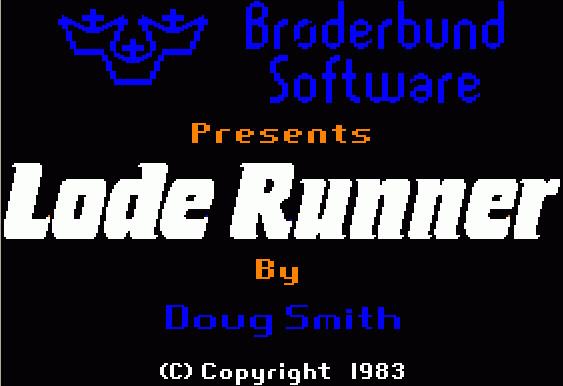
\includegraphics[width=\columnwidth]{title-screen}
\end{center}

You control the movement of your character, moving left and right along brick
and bedrock platforms, climbing ladders,
and "monkey-traversing" ropes strung across gaps. The object is to collect all the
gold boxes while avoiding being touched by the guards. You can dig holes in
brick parts of the floor which can allow you to reach otherwise unreachable caverns,
and the holes can also trap the guards for a short while. Holes fill themselves in
after a short time period, and if you're in a hole when that happens, you lose
a life. However, if a guard is in the hole and the hole fills, the guard disappears and
reappears somewhere along the top of the screen.

You get points for collecting boxes and forcing guards to respawn. Once you collect
all the boxes, a ladder will appear leading out of the top of the screen. This
gets you to the next level, and play continues.

\begin{center}
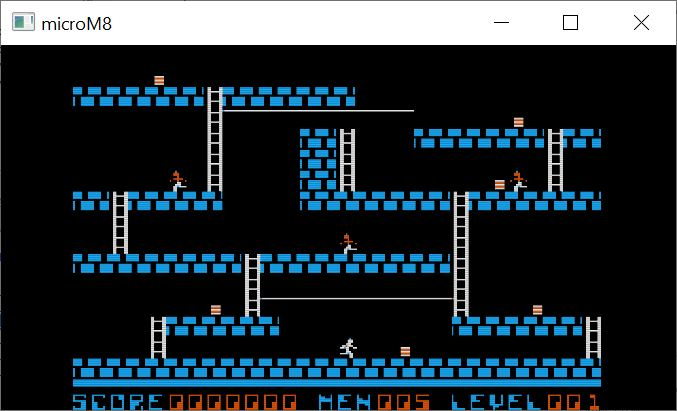
\includegraphics[width=\columnwidth]{screen}
\end{center}

Lode Runner included 150 levels and also a level editor.

\section{About this document}

This is a literate programming document. This means the explanatory text is
interspersed with source code. The source code can be extracted from the document
and compiled.

The goal is to provide all the source code necessary to reproduce a binary
identical to the one found on the Internet Archive's {\Tt{}Lode{\_}Runner{\_}1983{\_}Broderbund{\_}cr{\_}Reset{\_}Vector.do\nwendquote}
disk image.

The assembly code is assembled using {\Tt{}dasm\nwendquote}.

This document doesn't explain every last detail. It's assumed that the reader can
find enough details on the 6502 processor and the Apple II series of computers
to fill in the gaps.

\chapter{Programming techniques}

\section{Zero page temporaries}

Zero-page consists essentially of global variables. Sometimes we need local
temporaries, and Lode Runner mostly doesn't use the stack for those. Rather,
some "global" variables are reserved for temporaries. You might see multiple
symbols equated to a single zero-page location. The names of such symbols are
used to make sense within their context.

\section{Tail calls}

Rather than a {\Tt{}JSR\nwendquote} immediately followed by an {\Tt{}RTS\nwendquote}, instead a {\Tt{}JMP\nwendquote}
can be used to save stack space, code space, and time. This is known as a
tail call, because it is a call that happens at the tail of a function.

\section{Unconditional branches}

The 6502 doesn't have an unconditional short jump. However, if you can find
a condition that is always true, this can serve as an unconditional short
jump, which saves space and time.

\section{Stretchy branches}

6502 branches have a limit to how far they can jump. If they really need to
jump farther than that, you have to put a {\Tt{}JMP\nwendquote} or an unconditional branch
within reach.

\section{Shared code}

To save space, sometimes code at the end of one function is also useful to
the next function, as long as it is within reach. This can save space, at
the expense of functions being completely independent.

\section{DOS}

Since programs generally come on disk, and such disks are genrally bootable,
the only thing the disk card does is load the data of the disk on track 0
sector 0 to location {\Tt{}0800\nwendquote} and then jump to it. Thus, any additional
services need to be supplied by the disk as a disk operating system. The most
popular ones were DOS 3.3 and ProDOS.

Lode Runner contains just the parts of DOS 3.3 it needs. See the section on
Disk routines for more information.

\section{Temporaries and scratch space}

\nwenddocs{}\nwbegincode{2}\sublabel{NW1Xx3lK-10jlgu-1}\nwmargintag{{\nwtagstyle{}\subpageref{NW1Xx3lK-10jlgu-1}}}\moddef{defines~{\nwtagstyle{}\subpageref{NW1Xx3lK-10jlgu-1}}}\endmoddef\nwstartdeflinemarkup\nwusesondefline{\\{NW1Xx3lK-1p0Y9w-1}}\nwprevnextdefs{\relax}{NW1Xx3lK-10jlgu-2}\nwenddeflinemarkup
\nwlinkedidentc{TMP_PTR}{NW1Xx3lK-10jlgu-1}             EQU     $0A     ; 2 bytes
\nwlinkedidentc{TMP}{NW1Xx3lK-10jlgu-1}                 EQU     $1A
\nwlinkedidentc{SCRATCH_5C}{NW1Xx3lK-10jlgu-1}          EQU     $5C
\nwlinkedidentc{MATH_TMPL}{NW1Xx3lK-10jlgu-1}           EQU     $6F
\nwlinkedidentc{MATH_TMPH}{NW1Xx3lK-10jlgu-1}           EQU     $70
\nwlinkedidentc{TMP_LOOP_CTR}{NW1Xx3lK-10jlgu-1}        EQU     $88
\nwlinkedidentc{SCRATCH_A1}{NW1Xx3lK-10jlgu-1}          EQU     $A1
\nwindexdefn{\nwixident{TMP{\_}PTR}}{TMP:unPTR}{NW1Xx3lK-10jlgu-1}\nwindexdefn{\nwixident{TMP}}{TMP}{NW1Xx3lK-10jlgu-1}\nwindexdefn{\nwixident{SCRATCH{\_}5C}}{SCRATCH:un5C}{NW1Xx3lK-10jlgu-1}\nwindexdefn{\nwixident{TMP{\_}LOOP{\_}CTR}}{TMP:unLOOP:unCTR}{NW1Xx3lK-10jlgu-1}\nwindexdefn{\nwixident{SCRATCH{\_}A1}}{SCRATCH:unA1}{NW1Xx3lK-10jlgu-1}\nwindexdefn{\nwixident{MATH{\_}TMPL}}{MATH:unTMPL}{NW1Xx3lK-10jlgu-1}\nwindexdefn{\nwixident{MATH{\_}TMPH}}{MATH:unTMPH}{NW1Xx3lK-10jlgu-1}\eatline
\nwalsodefined{\\{NW1Xx3lK-10jlgu-2}\\{NW1Xx3lK-10jlgu-3}\\{NW1Xx3lK-10jlgu-4}\\{NW1Xx3lK-10jlgu-5}\\{NW1Xx3lK-10jlgu-6}\\{NW1Xx3lK-10jlgu-7}\\{NW1Xx3lK-10jlgu-8}\\{NW1Xx3lK-10jlgu-9}\\{NW1Xx3lK-10jlgu-A}\\{NW1Xx3lK-10jlgu-B}\\{NW1Xx3lK-10jlgu-C}\\{NW1Xx3lK-10jlgu-D}\\{NW1Xx3lK-10jlgu-E}\\{NW1Xx3lK-10jlgu-F}\\{NW1Xx3lK-10jlgu-G}\\{NW1Xx3lK-10jlgu-H}\\{NW1Xx3lK-10jlgu-I}\\{NW1Xx3lK-10jlgu-J}\\{NW1Xx3lK-10jlgu-K}\\{NW1Xx3lK-10jlgu-L}\\{NW1Xx3lK-10jlgu-M}\\{NW1Xx3lK-10jlgu-N}\\{NW1Xx3lK-10jlgu-O}\\{NW1Xx3lK-10jlgu-P}\\{NW1Xx3lK-10jlgu-Q}\\{NW1Xx3lK-10jlgu-R}\\{NW1Xx3lK-10jlgu-S}\\{NW1Xx3lK-10jlgu-T}\\{NW1Xx3lK-10jlgu-U}\\{NW1Xx3lK-10jlgu-V}\\{NW1Xx3lK-10jlgu-W}\\{NW1Xx3lK-10jlgu-X}\\{NW1Xx3lK-10jlgu-Y}\\{NW1Xx3lK-10jlgu-Z}\\{NW1Xx3lK-10jlgu-a}\\{NW1Xx3lK-10jlgu-b}\\{NW1Xx3lK-10jlgu-c}\\{NW1Xx3lK-10jlgu-d}\\{NW1Xx3lK-10jlgu-e}\\{NW1Xx3lK-10jlgu-f}\\{NW1Xx3lK-10jlgu-g}\\{NW1Xx3lK-10jlgu-h}\\{NW1Xx3lK-10jlgu-i}\\{NW1Xx3lK-10jlgu-j}\\{NW1Xx3lK-10jlgu-k}\\{NW1Xx3lK-10jlgu-l}\\{NW1Xx3lK-10jlgu-m}\\{NW1Xx3lK-10jlgu-n}\\{NW1Xx3lK-10jlgu-o}\\{NW1Xx3lK-10jlgu-p}}\nwused{\\{NW1Xx3lK-1p0Y9w-1}}\nwidentdefs{\\{{\nwixident{MATH{\_}TMPH}}{MATH:unTMPH}}\\{{\nwixident{MATH{\_}TMPL}}{MATH:unTMPL}}\\{{\nwixident{SCRATCH{\_}5C}}{SCRATCH:un5C}}\\{{\nwixident{SCRATCH{\_}A1}}{SCRATCH:unA1}}\\{{\nwixident{TMP}}{TMP}}\\{{\nwixident{TMP{\_}LOOP{\_}CTR}}{TMP:unLOOP:unCTR}}\\{{\nwixident{TMP{\_}PTR}}{TMP:unPTR}}}\nwendcode{}\nwbegindocs{3}\nwdocspar
\chapter{Apple II Graphics}
Hi-res graphics on the Apple II is odd. Graphics are memory-mapped, not exactly
consecutively, and bits don't always correspond to pixels. Color especially is
odd, compared to today's luxurious 32-bit per pixel RGBA.

The Apple II has two hi-res graphics pages, and maps the area from {\Tt{}{\$}2000-{\$}3FFF\nwendquote} to
high-res graphics page 1 (HGR1), and {\Tt{}{\$}4000-{\$}5FFF\nwendquote} to page 2 (HGR2).

We have routines to clear these screens.

\nwenddocs{}\nwbegincode{4}\sublabel{NW1Xx3lK-8jv1b-1}\nwmargintag{{\nwtagstyle{}\subpageref{NW1Xx3lK-8jv1b-1}}}\moddef{routines~{\nwtagstyle{}\subpageref{NW1Xx3lK-8jv1b-1}}}\endmoddef\nwstartdeflinemarkup\nwusesondefline{\\{NW1Xx3lK-1p0Y9w-1}}\nwprevnextdefs{\relax}{NW1Xx3lK-8jv1b-2}\nwenddeflinemarkup
    ORG     $7A51
\nwlinkedidentc{CLEAR_HGR1}{NW1Xx3lK-8jv1b-1}:
    SUBROUTINE

    LDA     #$20                ; Start at $2000
    LDX     #$40                ; End at $4000 (but not including)
    BNE     CLEAR_PAGE          ; Unconditional jump

\nwlinkedidentc{CLEAR_HGR2}{NW1Xx3lK-8jv1b-1}:
    SUBROUTINE

    LDA     #$40                ; Start at $4000
    LDX     #$60                ; End at $6000 (but not including)
    ; fallthrough

CLEAR_PAGE:
    STA     \nwlinkedidentc{TMP_PTR}{NW1Xx3lK-10jlgu-1}+1           ; Start with the page in A.
    LDA     #$00
    STA     \nwlinkedidentc{TMP_PTR}{NW1Xx3lK-10jlgu-1}
    TAY
    LDA     #$80                ; fill byte = 0x80

.loop:
    STA     (\nwlinkedidentc{TMP_PTR}{NW1Xx3lK-10jlgu-1}),Y
    INY
    BNE     .loop
    INC     \nwlinkedidentc{TMP_PTR}{NW1Xx3lK-10jlgu-1}+1
    CPX     \nwlinkedidentc{TMP_PTR}{NW1Xx3lK-10jlgu-1}+1
    BNE     .loop               ; while \nwlinkedidentc{TMP_PTR}{NW1Xx3lK-10jlgu-1} != X * 0x100
    RTS
\nwindexdefn{\nwixident{CLEAR{\_}HGR1}}{CLEAR:unHGR1}{NW1Xx3lK-8jv1b-1}\nwindexdefn{\nwixident{CLEAR{\_}HGR2}}{CLEAR:unHGR2}{NW1Xx3lK-8jv1b-1}\eatline
\nwalsodefined{\\{NW1Xx3lK-8jv1b-2}\\{NW1Xx3lK-8jv1b-3}\\{NW1Xx3lK-8jv1b-4}\\{NW1Xx3lK-8jv1b-5}\\{NW1Xx3lK-8jv1b-6}\\{NW1Xx3lK-8jv1b-7}\\{NW1Xx3lK-8jv1b-8}\\{NW1Xx3lK-8jv1b-9}\\{NW1Xx3lK-8jv1b-A}\\{NW1Xx3lK-8jv1b-B}\\{NW1Xx3lK-8jv1b-C}}\nwused{\\{NW1Xx3lK-1p0Y9w-1}}\nwidentdefs{\\{{\nwixident{CLEAR{\_}HGR1}}{CLEAR:unHGR1}}\\{{\nwixident{CLEAR{\_}HGR2}}{CLEAR:unHGR2}}}\nwidentuses{\\{{\nwixident{TMP{\_}PTR}}{TMP:unPTR}}}\nwindexuse{\nwixident{TMP{\_}PTR}}{TMP:unPTR}{NW1Xx3lK-8jv1b-1}\nwendcode{}\nwbegindocs{5}\nwdocspar
\section{Pixels and their color}
First we'll talk about pixels. Nominally, the resolution of the hi-res graphics screen
is 280 pixels wide by 192 pixels tall. In the memory map, each row is represented
by 40 bytes. The high bit of each byte is not used for pixel data, but is used to
control color.

Here are some rules for how these bytes are turned into pixels:
\begin{itemize}
  \item Pixels are drawn to the screen from byte data least significant bit first.
        This means that for the first byte bit 0 is column 0, bit 1 is column 1,
        and so on.
  \item A pattern of {\Tt{}11\nwendquote} results in two white pixels at the {\Tt{}1\nwendquote} positions.
  \item A pattern of {\Tt{}010\nwendquote} results at least in a colored pixel at the {\Tt{}1\nwendquote} position.
  \item A pattern of {\Tt{}101\nwendquote} results at least in a colored pixel at the {\Tt{}0\nwendquote} position.
  \item So, a pattern of {\Tt{}01010\nwendquote} results in at least three consecutive colored
        pixels starting from the first {\Tt{}1\nwendquote} to the last {\Tt{}1\nwendquote}. The last {\Tt{}0\nwendquote} bit
        would also be colored if followed by a {\Tt{}1\nwendquote}.
  \item Likewise, a pattern of {\Tt{}11011\nwendquote} results in two white pixels, a colored pixel,
        and then two more white pixels.
  \item The color of a {\Tt{}010\nwendquote} pixel depends on the column that the {\Tt{}1\nwendquote} falls on, and
        also whether the high bit of its byte was set or not. 
  \item The color of a {\Tt{}11011\nwendquote} pixel depends on the column that the {\Tt{}0\nwendquote} falls on, and
        also whether the high bit of its byte was set or not.

        \begin{center}
        \begin{tabular}{@{}rcc@{}} \toprule
        & Odd & Even \\ \cmidrule(r){2-3}
        High bit clear & Green & Violet \\
        High bit set & Orange & Blue \\ \bottomrule
        \end{tabular}
        \end{center}

        The implication is that you can only select one pair of colors per byte.
\end{itemize}

An example would probably be good here. We will take one of the sprites from the game.

\begin{center}
\begin{tabular}{@{}rcc@{}} \toprule
Bytes & Bits & Pixel Data \\ \cmidrule{1-3}
{\Tt{}00\ 00\nwendquote} & {\Tt{}0000000\ 0000000\nwendquote} & {\Tt{}00000000000000\nwendquote} \\
{\Tt{}00\ 00\nwendquote} & {\Tt{}0000000\ 0000000\nwendquote} & {\Tt{}00000000000000\nwendquote} \\
{\Tt{}00\ 00\nwendquote} & {\Tt{}0000000\ 0000000\nwendquote} & {\Tt{}00000000000000\nwendquote} \\
{\Tt{}55\ 00\nwendquote} & {\Tt{}1010101\ 0000000\nwendquote} & {\Tt{}10101010000000\nwendquote} \\
{\Tt{}41\ 00\nwendquote} & {\Tt{}1000001\ 0000000\nwendquote} & {\Tt{}10000010000000\nwendquote} \\
{\Tt{}01\ 00\nwendquote} & {\Tt{}0000001\ 0000000\nwendquote} & {\Tt{}10000000000000\nwendquote} \\
{\Tt{}55\ 00\nwendquote} & {\Tt{}1010101\ 0000000\nwendquote} & {\Tt{}10101010000000\nwendquote} \\
{\Tt{}50\ 00\nwendquote} & {\Tt{}1010000\ 0000000\nwendquote} & {\Tt{}00001010000000\nwendquote} \\
{\Tt{}50\ 00\nwendquote} & {\Tt{}1010000\ 0000000\nwendquote} & {\Tt{}00001010000000\nwendquote} \\
{\Tt{}51\ 00\nwendquote} & {\Tt{}1010001\ 0000000\nwendquote} & {\Tt{}10001010000000\nwendquote} \\
{\Tt{}55\ 00\nwendquote} & {\Tt{}1010101\ 0000000\nwendquote} & {\Tt{}10101010000000\nwendquote} \\ \bottomrule
\end{tabular}
\end{center}

The game automatically sets the high bit of each byte, so we know we're going to see
orange and blue. Assuming that the following bits are all zero, and we place the
sprite starting at column 0, we should see this:

\begin{center}
\begin{tabular}{@{}rcccccccccccccc@{}}
 0 & \bk0 & \bk0 & \bk0 & \bk0 & \bk0 & \bk0 & \bk0 & \bk0 & \bk0 & \bk0 & \bk0 & \bk0 & \bk0 & \bk0 \\
 1 & \bk0 & \bk0 & \bk0 & \bk0 & \bk0 & \bk0 & \bk0 & \bk0 & \bk0 & \bk0 & \bk0 & \bk0 & \bk0 & \bk0 \\
 2 & \bk0 & \bk0 & \bk0 & \bk0 & \bk0 & \bk0 & \bk0 & \bk0 & \bk0 & \bk0 & \bk0 & \bk0 & \bk0 & \bk0 \\
 3 & \bl0 & \bl0 & \bl0 & \bl0 & \bl0 & \bl0 & \bl0 & \bk0 & \bk0 & \bk0 & \bk0 & \bk0 & \bk0 & \bk0 \\
 4 & \bl0 & \bk0 & \bk0 & \bk0 & \bk0 & \bk0 & \bl0 & \bk0 & \bk0 & \bk0 & \bk0 & \bk0 & \bk0 & \bk0 \\
 5 & \bl0 & \bk0 & \bk0 & \bk0 & \bk0 & \bk0 & \bk0 & \bk0 & \bk0 & \bk0 & \bk0 & \bk0 & \bk0 & \bk0 \\
 6 & \bl0 & \bl0 & \bl0 & \bl0 & \bl0 & \bl0 & \bl0 & \bk0 & \bk0 & \bk0 & \bk0 & \bk0 & \bk0 & \bk0 \\
 7 & \bk0 & \bk0 & \bk0 & \bk0 & \bl0 & \bl0 & \bl0 & \bk0 & \bk0 & \bk0 & \bk0 & \bk0 & \bk0 & \bk0 \\
 8 & \bk0 & \bk0 & \bk0 & \bk0 & \bl0 & \bl0 & \bl0 & \bk0 & \bk0 & \bk0 & \bk0 & \bk0 & \bk0 & \bk0 \\
 9 & \bl0 & \bk0 & \bk0 & \bk0 & \bl0 & \bl0 & \bl0 & \bk0 & \bk0 & \bk0 & \bk0 & \bk0 & \bk0 & \bk0 \\
10 & \bl0 & \bl0 & \bl0 & \bl0 & \bl0 & \bl0 & \bl0 & \bk0 & \bk0 & \bk0 & \bk0 & \bk0 & \bk0 & \bk0 \\
\end{tabular}
\end{center}

Here is a more complex sprite:

\begin{center}
\begin{tabular}{@{}rcc@{}} \toprule
Bytes & Bits & Pixel Data \\ \cmidrule{1-3}
{\Tt{}40\ 00\nwendquote} & {\Tt{}1000000\ 0000000\nwendquote} & {\Tt{}00000010000000\nwendquote} \\
{\Tt{}60\ 01\nwendquote} & {\Tt{}1100000\ 0000001\nwendquote} & {\Tt{}00000111000000\nwendquote} \\
{\Tt{}60\ 01\nwendquote} & {\Tt{}1100000\ 0000001\nwendquote} & {\Tt{}00000111000000\nwendquote} \\
{\Tt{}70\ 00\nwendquote} & {\Tt{}1110000\ 0000000\nwendquote} & {\Tt{}00001110000000\nwendquote} \\
{\Tt{}6C\ 01\nwendquote} & {\Tt{}1101100\ 0000001\nwendquote} & {\Tt{}00110111000000\nwendquote} \\
{\Tt{}36\ 06\nwendquote} & {\Tt{}0110110\ 0000110\nwendquote} & {\Tt{}01101100110000\nwendquote} \\
{\Tt{}30\ 00\nwendquote} & {\Tt{}0110000\ 0000000\nwendquote} & {\Tt{}00001100000000\nwendquote} \\
{\Tt{}70\ 00\nwendquote} & {\Tt{}1110000\ 0000000\nwendquote} & {\Tt{}00001110000000\nwendquote} \\
{\Tt{}5E\ 01\nwendquote} & {\Tt{}1011110\ 0000001\nwendquote} & {\Tt{}01111011000000\nwendquote} \\
{\Tt{}40\ 01\nwendquote} & {\Tt{}1000000\ 0000001\nwendquote} & {\Tt{}00000011000000\nwendquote} \\
{\Tt{}40\ 01\nwendquote} & {\Tt{}1000000\ 0000001\nwendquote} & {\Tt{}00000011000000\nwendquote} \\ \bottomrule
\end{tabular}
\end{center}

\begin{center}
\begin{tabular}{@{}rcccccccccccccc@{}}
0 & \bk0 & \bk0 & \bk0 & \bk0 & \bk0 & \bk0 & \bl0 & \bk0 & \bk0 & \bk0 & \bk0 & \bk0 & \bk0 & \bk0 \\
1 & \bk0 & \bk0 & \bk0 & \bk0 & \bk0 & \bw0 & \bw0 & \bw0 & \bk0 & \bk0 & \bk0 & \bk0 & \bk0 & \bk0 \\
2 & \bk0 & \bk0 & \bk0 & \bk0 & \bk0 & \bw0 & \bw0 & \bw0 & \bk0 & \bk0 & \bk0 & \bk0 & \bk0 & \bk0 \\
3 & \bk0 & \bk0 & \bk0 & \bk0 & \bw0 & \bw0 & \bw0 & \bk0 & \bk0 & \bk0 & \bk0 & \bk0 & \bk0 & \bk0 \\
4 & \bk0 & \bk0 & \bw0 & \bw0 & \bo0 & \bw0 & \bw0 & \bw0 & \bk0 & \bk0 & \bk0 & \bk0 & \bk0 & \bk0 \\
5 & \bk0 & \bw0 & \bw0 & \bl0 & \bw0 & \bw0 & \bk0 & \bk0 & \bw0 & \bw0 & \bk0 & \bk0 & \bk0 & \bk0 \\
6 & \bk0 & \bk0 & \bk0 & \bk0 & \bw0 & \bw0 & \bk0 & \bk0 & \bk0 & \bk0 & \bk0 & \bk0 & \bk0 & \bk0 \\
7 & \bk0 & \bk0 & \bk0 & \bk0 & \bw0 & \bw0 & \bw0 & \bk0 & \bk0 & \bk0 & \bk0 & \bk0 & \bk0 & \bk0 \\
8 & \bk0 & \bw0 & \bw0 & \bw0 & \bw0 & \bl0 & \bw0 & \bw0 & \bk0 & \bk0 & \bk0 & \bk0 & \bk0 & \bk0 \\
9 & \bk0 & \bk0 & \bk0 & \bk0 & \bk0 & \bk0 & \bw0 & \bw0 & \bk0 & \bk0 & \bk0 & \bk0 & \bk0 & \bk0 \\
10 & \bk0 & \bk0 & \bk0 & \bk0 & \bk0 & \bk0 & \bw0 & \bw0 & \bk0 & \bk0 & \bk0 & \bk0 & \bk0 & \bk0 \\
\end{tabular}
\end{center}

Take note of the orange and blue pixels. All the patterns noted in the rules above are used.

\section{The sprites}
Lode Runner defines 104 sprites, each being 11 rows, with two bytes per row. The first bytes of
all 104 sprites are in the table first, then the second bytes, then the third bytes, and so on.
Later we will see that only the leftmost 10 pixels out of the 14-pixel description is used.

\nwenddocs{}\nwbegincode{6}\sublabel{NW1Xx3lK-1W8AJS-1}\nwmargintag{{\nwtagstyle{}\subpageref{NW1Xx3lK-1W8AJS-1}}}\moddef{tables~{\nwtagstyle{}\subpageref{NW1Xx3lK-1W8AJS-1}}}\endmoddef\nwstartdeflinemarkup\nwusesondefline{\\{NW1Xx3lK-1p0Y9w-1}}\nwprevnextdefs{\relax}{NW1Xx3lK-1W8AJS-2}\nwenddeflinemarkup
    ORG     $AD00
\nwlinkedidentc{SPRITE_DATA}{NW1Xx3lK-1W8AJS-1}:
    INCLUDE "sprite_data.asm"
\nwindexdefn{\nwixident{SPRITE{\_}DATA}}{SPRITE:unDATA}{NW1Xx3lK-1W8AJS-1}\eatline
\nwalsodefined{\\{NW1Xx3lK-1W8AJS-2}\\{NW1Xx3lK-1W8AJS-3}\\{NW1Xx3lK-1W8AJS-4}\\{NW1Xx3lK-1W8AJS-5}\\{NW1Xx3lK-1W8AJS-6}\\{NW1Xx3lK-1W8AJS-7}\\{NW1Xx3lK-1W8AJS-8}\\{NW1Xx3lK-1W8AJS-9}\\{NW1Xx3lK-1W8AJS-A}\\{NW1Xx3lK-1W8AJS-B}\\{NW1Xx3lK-1W8AJS-C}\\{NW1Xx3lK-1W8AJS-D}\\{NW1Xx3lK-1W8AJS-E}\\{NW1Xx3lK-1W8AJS-F}\\{NW1Xx3lK-1W8AJS-G}\\{NW1Xx3lK-1W8AJS-H}\\{NW1Xx3lK-1W8AJS-I}\\{NW1Xx3lK-1W8AJS-J}\\{NW1Xx3lK-1W8AJS-K}\\{NW1Xx3lK-1W8AJS-L}\\{NW1Xx3lK-1W8AJS-M}\\{NW1Xx3lK-1W8AJS-N}\\{NW1Xx3lK-1W8AJS-O}\\{NW1Xx3lK-1W8AJS-P}\\{NW1Xx3lK-1W8AJS-Q}\\{NW1Xx3lK-1W8AJS-R}\\{NW1Xx3lK-1W8AJS-S}\\{NW1Xx3lK-1W8AJS-T}\\{NW1Xx3lK-1W8AJS-U}\\{NW1Xx3lK-1W8AJS-V}\\{NW1Xx3lK-1W8AJS-W}\\{NW1Xx3lK-1W8AJS-X}}\nwused{\\{NW1Xx3lK-1p0Y9w-1}}\nwidentdefs{\\{{\nwixident{SPRITE{\_}DATA}}{SPRITE:unDATA}}}\nwendcode{}\nwbegindocs{7}\nwdocspar
\begin{center}
\scalebox{0.8}{
\begin{tabular}{@{}rcccccccccccccccccccccccccccccc@{}}
 & \multicolumn{14}{c}{Sprite 0} & & \multicolumn{14}{c}{Sprite 1} \\
0 & \bk0 & \bk0 & \bk0 & \bk0 & \bk0 & \bk0 & \bk0 & \bk0 & \bk0 & \bk0 & \bk0 & \bk0 & \bk0 & \bk0 & & \bl0 & \bl0 & \bl0 & \bl0 & \bl0 & \bk0 & \bk0 & \bk0 & \bl0 & \bk0 & \bk0 & \bk0 & \bk0 & \bk0 & \\
1 & \bk0 & \bk0 & \bk0 & \bk0 & \bk0 & \bk0 & \bk0 & \bk0 & \bk0 & \bk0 & \bk0 & \bk0 & \bk0 & \bk0 & & \bl0 & \bl0 & \bl0 & \bl0 & \bl0 & \bk0 & \bk0 & \bk0 & \bl0 & \bk0 & \bk0 & \bk0 & \bk0 & \bk0 & \\
2 & \bk0 & \bk0 & \bk0 & \bk0 & \bk0 & \bk0 & \bk0 & \bk0 & \bk0 & \bk0 & \bk0 & \bk0 & \bk0 & \bk0 & & \bl0 & \bl0 & \bl0 & \bl0 & \bl0 & \bk0 & \bk0 & \bk0 & \bl0 & \bk0 & \bk0 & \bk0 & \bk0 & \bk0 & \\
3 & \bk0 & \bk0 & \bk0 & \bk0 & \bk0 & \bk0 & \bk0 & \bk0 & \bk0 & \bk0 & \bk0 & \bk0 & \bk0 & \bk0 & & \bl0 & \bl0 & \bl0 & \bl0 & \bl0 & \bk0 & \bk0 & \bk0 & \bl0 & \bk0 & \bk0 & \bk0 & \bk0 & \bk0 & \\
4 & \bk0 & \bk0 & \bk0 & \bk0 & \bk0 & \bk0 & \bk0 & \bk0 & \bk0 & \bk0 & \bk0 & \bk0 & \bk0 & \bk0 & & \bk0 & \bk0 & \bk0 & \bk0 & \bk0 & \bk0 & \bk0 & \bk0 & \bk0 & \bk0 & \bk0 & \bk0 & \bk0 & \bk0 & \\
5 & \bk0 & \bk0 & \bk0 & \bk0 & \bk0 & \bk0 & \bk0 & \bk0 & \bk0 & \bk0 & \bk0 & \bk0 & \bk0 & \bk0 & & \bl0 & \bk0 & \bk0 & \bk0 & \bl0 & \bl0 & \bl0 & \bl0 & \bl0 & \bk0 & \bk0 & \bk0 & \bk0 & \bk0 & \\
6 & \bk0 & \bk0 & \bk0 & \bk0 & \bk0 & \bk0 & \bk0 & \bk0 & \bk0 & \bk0 & \bk0 & \bk0 & \bk0 & \bk0 & & \bl0 & \bk0 & \bk0 & \bk0 & \bl0 & \bl0 & \bl0 & \bl0 & \bl0 & \bk0 & \bk0 & \bk0 & \bk0 & \bk0 & \\
7 & \bk0 & \bk0 & \bk0 & \bk0 & \bk0 & \bk0 & \bk0 & \bk0 & \bk0 & \bk0 & \bk0 & \bk0 & \bk0 & \bk0 & & \bl0 & \bk0 & \bk0 & \bk0 & \bl0 & \bl0 & \bl0 & \bl0 & \bl0 & \bk0 & \bk0 & \bk0 & \bk0 & \bk0 & \\
8 & \bk0 & \bk0 & \bk0 & \bk0 & \bk0 & \bk0 & \bk0 & \bk0 & \bk0 & \bk0 & \bk0 & \bk0 & \bk0 & \bk0 & & \bl0 & \bk0 & \bk0 & \bk0 & \bl0 & \bl0 & \bl0 & \bl0 & \bl0 & \bk0 & \bk0 & \bk0 & \bk0 & \bk0 & \\
9 & \bk0 & \bk0 & \bk0 & \bk0 & \bk0 & \bk0 & \bk0 & \bk0 & \bk0 & \bk0 & \bk0 & \bk0 & \bk0 & \bk0 & & \bl0 & \bk0 & \bk0 & \bk0 & \bl0 & \bl0 & \bl0 & \bl0 & \bl0 & \bk0 & \bk0 & \bk0 & \bk0 & \bk0 & \\
10 & \bk0 & \bk0 & \bk0 & \bk0 & \bk0 & \bk0 & \bk0 & \bk0 & \bk0 & \bk0 & \bk0 & \bk0 & \bk0 & \bk0 & & \bk0 & \bk0 & \bk0 & \bk0 & \bk0 & \bk0 & \bk0 & \bk0 & \bk0 & \bk0 & \bk0 & \bk0 & \bk0 & \bk0 & \\
\end{tabular}
}
\end{center}
\begin{center}
\scalebox{0.8}{
\begin{tabular}{@{}rcccccccccccccccccccccccccccccc@{}}
 & \multicolumn{14}{c}{Sprite 2} & & \multicolumn{14}{c}{Sprite 3} \\
0 & \bl0 & \bl0 & \bl0 & \bl0 & \bl0 & \bl0 & \bl0 & \bl0 & \bl0 & \bk0 & \bk0 & \bk0 & \bk0 & \bk0 & & \bk0 & \bw0 & \bw0 & \bk0 & \bk0 & \bk0 & \bk0 & \bw0 & \bw0 & \bk0 & \bk0 & \bk0 & \bk0 & \bk0 & \\
1 & \bl0 & \bl0 & \bl0 & \bl0 & \bl0 & \bl0 & \bl0 & \bl0 & \bl0 & \bk0 & \bk0 & \bk0 & \bk0 & \bk0 & & \bk0 & \bw0 & \bw0 & \bk0 & \bk0 & \bk0 & \bk0 & \bw0 & \bw0 & \bk0 & \bk0 & \bk0 & \bk0 & \bk0 & \\
2 & \bl0 & \bl0 & \bl0 & \bl0 & \bl0 & \bl0 & \bl0 & \bl0 & \bl0 & \bk0 & \bk0 & \bk0 & \bk0 & \bk0 & & \bk0 & \bw0 & \bw0 & \bw0 & \bw0 & \bw0 & \bw0 & \bw0 & \bw0 & \bk0 & \bk0 & \bk0 & \bk0 & \bk0 & \\
3 & \bl0 & \bl0 & \bl0 & \bl0 & \bl0 & \bl0 & \bl0 & \bl0 & \bl0 & \bk0 & \bk0 & \bk0 & \bk0 & \bk0 & & \bk0 & \bw0 & \bw0 & \bk0 & \bk0 & \bk0 & \bk0 & \bw0 & \bw0 & \bk0 & \bk0 & \bk0 & \bk0 & \bk0 & \\
4 & \bl0 & \bl0 & \bl0 & \bl0 & \bl0 & \bl0 & \bl0 & \bl0 & \bl0 & \bk0 & \bk0 & \bk0 & \bk0 & \bk0 & & \bk0 & \bw0 & \bw0 & \bk0 & \bk0 & \bk0 & \bk0 & \bw0 & \bw0 & \bk0 & \bk0 & \bk0 & \bk0 & \bk0 & \\
5 & \bl0 & \bl0 & \bl0 & \bl0 & \bl0 & \bl0 & \bl0 & \bl0 & \bl0 & \bk0 & \bk0 & \bk0 & \bk0 & \bk0 & & \bk0 & \bw0 & \bw0 & \bk0 & \bk0 & \bk0 & \bk0 & \bw0 & \bw0 & \bk0 & \bk0 & \bk0 & \bk0 & \bk0 & \\
6 & \bl0 & \bl0 & \bl0 & \bl0 & \bl0 & \bl0 & \bl0 & \bl0 & \bl0 & \bk0 & \bk0 & \bk0 & \bk0 & \bk0 & & \bk0 & \bw0 & \bw0 & \bk0 & \bk0 & \bk0 & \bk0 & \bw0 & \bw0 & \bk0 & \bk0 & \bk0 & \bk0 & \bk0 & \\
7 & \bl0 & \bl0 & \bl0 & \bl0 & \bl0 & \bl0 & \bl0 & \bl0 & \bl0 & \bk0 & \bk0 & \bk0 & \bk0 & \bk0 & & \bk0 & \bw0 & \bw0 & \bw0 & \bw0 & \bw0 & \bw0 & \bw0 & \bw0 & \bk0 & \bk0 & \bk0 & \bk0 & \bk0 & \\
8 & \bl0 & \bl0 & \bl0 & \bl0 & \bl0 & \bl0 & \bl0 & \bl0 & \bl0 & \bk0 & \bk0 & \bk0 & \bk0 & \bk0 & & \bk0 & \bw0 & \bw0 & \bk0 & \bk0 & \bk0 & \bk0 & \bw0 & \bw0 & \bk0 & \bk0 & \bk0 & \bk0 & \bk0 & \\
9 & \bl0 & \bl0 & \bl0 & \bl0 & \bl0 & \bl0 & \bl0 & \bl0 & \bl0 & \bk0 & \bk0 & \bk0 & \bk0 & \bk0 & & \bk0 & \bw0 & \bw0 & \bk0 & \bk0 & \bk0 & \bk0 & \bw0 & \bw0 & \bk0 & \bk0 & \bk0 & \bk0 & \bk0 & \\
10 & \bk0 & \bk0 & \bk0 & \bk0 & \bk0 & \bk0 & \bk0 & \bk0 & \bk0 & \bk0 & \bk0 & \bk0 & \bk0 & \bk0 & & \bk0 & \bw0 & \bw0 & \bk0 & \bk0 & \bk0 & \bk0 & \bw0 & \bw0 & \bk0 & \bk0 & \bk0 & \bk0 & \bk0 & \\
\end{tabular}
}
\end{center}
\begin{center}
\scalebox{0.8}{
\begin{tabular}{@{}rcccccccccccccccccccccccccccccc@{}}
 & \multicolumn{14}{c}{Sprite 4} & & \multicolumn{14}{c}{Sprite 5} \\
0 & \bk0 & \bk0 & \bk0 & \bk0 & \bk0 & \bk0 & \bk0 & \bk0 & \bk0 & \bk0 & \bk0 & \bk0 & \bk0 & \bk0 & & \bl0 & \bl0 & \bl0 & \bl0 & \bl0 & \bl0 & \bl0 & \bl0 & \bl0 & \bk0 & \bk0 & \bk0 & \bk0 & \bk0 & \\
1 & \bw0 & \bw0 & \bw0 & \bw0 & \bw0 & \bw0 & \bw0 & \bw0 & \bw0 & \bw0 & \bk0 & \bk0 & \bk0 & \bk0 & & \bl0 & \bl0 & \bl0 & \bl0 & \bl0 & \bl0 & \bl0 & \bl0 & \bl0 & \bk0 & \bk0 & \bk0 & \bk0 & \bk0 & \\
2 & \bk0 & \bk0 & \bk0 & \bk0 & \bk0 & \bk0 & \bk0 & \bk0 & \bk0 & \bk0 & \bk0 & \bk0 & \bk0 & \bk0 & & \bk0 & \bk0 & \bk0 & \bk0 & \bk0 & \bk0 & \bk0 & \bk0 & \bk0 & \bk0 & \bk0 & \bk0 & \bk0 & \bk0 & \\
3 & \bk0 & \bk0 & \bk0 & \bk0 & \bk0 & \bk0 & \bk0 & \bk0 & \bk0 & \bk0 & \bk0 & \bk0 & \bk0 & \bk0 & & \bk0 & \bk0 & \bw0 & \bw0 & \bw0 & \bw0 & \bw0 & \bw0 & \bk0 & \bk0 & \bk0 & \bk0 & \bk0 & \bk0 & \\
4 & \bk0 & \bk0 & \bk0 & \bk0 & \bk0 & \bk0 & \bk0 & \bk0 & \bk0 & \bk0 & \bk0 & \bk0 & \bk0 & \bk0 & & \bk0 & \bk0 & \bk0 & \bk0 & \bw0 & \bw0 & \bk0 & \bk0 & \bk0 & \bk0 & \bk0 & \bk0 & \bk0 & \bk0 & \\
5 & \bk0 & \bk0 & \bk0 & \bk0 & \bk0 & \bk0 & \bk0 & \bk0 & \bk0 & \bk0 & \bk0 & \bk0 & \bk0 & \bk0 & & \bk0 & \bk0 & \bk0 & \bk0 & \bw0 & \bw0 & \bk0 & \bk0 & \bk0 & \bk0 & \bk0 & \bk0 & \bk0 & \bk0 & \\
6 & \bk0 & \bk0 & \bk0 & \bk0 & \bk0 & \bk0 & \bk0 & \bk0 & \bk0 & \bk0 & \bk0 & \bk0 & \bk0 & \bk0 & & \bk0 & \bk0 & \bk0 & \bk0 & \bw0 & \bw0 & \bk0 & \bk0 & \bk0 & \bk0 & \bk0 & \bk0 & \bk0 & \bk0 & \\
7 & \bk0 & \bk0 & \bk0 & \bk0 & \bk0 & \bk0 & \bk0 & \bk0 & \bk0 & \bk0 & \bk0 & \bk0 & \bk0 & \bk0 & & \bk0 & \bk0 & \bk0 & \bk0 & \bw0 & \bw0 & \bk0 & \bk0 & \bk0 & \bk0 & \bk0 & \bk0 & \bk0 & \bk0 & \\
8 & \bk0 & \bk0 & \bk0 & \bk0 & \bk0 & \bk0 & \bk0 & \bk0 & \bk0 & \bk0 & \bk0 & \bk0 & \bk0 & \bk0 & & \bl0 & \bl0 & \bl0 & \bl0 & \bl0 & \bl0 & \bl0 & \bl0 & \bl0 & \bk0 & \bk0 & \bk0 & \bk0 & \bk0 & \\
9 & \bk0 & \bk0 & \bk0 & \bk0 & \bk0 & \bk0 & \bk0 & \bk0 & \bk0 & \bk0 & \bk0 & \bk0 & \bk0 & \bk0 & & \bl0 & \bl0 & \bl0 & \bl0 & \bl0 & \bl0 & \bl0 & \bl0 & \bl0 & \bk0 & \bk0 & \bk0 & \bk0 & \bk0 & \\
10 & \bk0 & \bk0 & \bk0 & \bk0 & \bk0 & \bk0 & \bk0 & \bk0 & \bk0 & \bk0 & \bk0 & \bk0 & \bk0 & \bk0 & & \bk0 & \bk0 & \bk0 & \bk0 & \bk0 & \bk0 & \bk0 & \bk0 & \bk0 & \bk0 & \bk0 & \bk0 & \bk0 & \bk0 & \\
\end{tabular}
}
\end{center}
\begin{center}
\scalebox{0.8}{
\begin{tabular}{@{}rcccccccccccccccccccccccccccccc@{}}
 & \multicolumn{14}{c}{Sprite 6} & & \multicolumn{14}{c}{Sprite 7} \\
0 & \bk0 & \bw0 & \bw0 & \bk0 & \bk0 & \bk0 & \bk0 & \bk0 & \bk0 & \bk0 & \bk0 & \bk0 & \bk0 & \bk0 & & \bk0 & \bk0 & \bk0 & \bk0 & \bk0 & \bk0 & \bk0 & \bk0 & \bk0 & \bk0 & \bk0 & \bk0 & \bk0 & \bk0 & \\
1 & \bk0 & \bw0 & \bw0 & \bk0 & \bk0 & \bk0 & \bk0 & \bk0 & \bk0 & \bk0 & \bk0 & \bk0 & \bk0 & \bk0 & & \bk0 & \bk0 & \bk0 & \bk0 & \bk0 & \bk0 & \bk0 & \bk0 & \bk0 & \bk0 & \bk0 & \bk0 & \bk0 & \bk0 & \\
2 & \bk0 & \bw0 & \bw0 & \bw0 & \bw0 & \bw0 & \bw0 & \bw0 & \bw0 & \bk0 & \bk0 & \bk0 & \bk0 & \bk0 & & \bk0 & \bk0 & \bk0 & \bk0 & \bk0 & \bk0 & \bk0 & \bk0 & \bk0 & \bk0 & \bk0 & \bk0 & \bk0 & \bk0 & \\
3 & \bk0 & \bw0 & \bw0 & \bk0 & \bk0 & \bk0 & \bk0 & \bw0 & \bw0 & \bk0 & \bk0 & \bk0 & \bk0 & \bk0 & & \bk0 & \bk0 & \bk0 & \bk0 & \bk0 & \bk0 & \bk0 & \bk0 & \bk0 & \bk0 & \bk0 & \bk0 & \bk0 & \bk0 & \\
4 & \bk0 & \bk0 & \bk0 & \bk0 & \bk0 & \bk0 & \bk0 & \bw0 & \bw0 & \bk0 & \bk0 & \bk0 & \bk0 & \bk0 & & \bk0 & \bk0 & \bk0 & \bk0 & \bk0 & \bk0 & \bk0 & \bk0 & \bk0 & \bk0 & \bk0 & \bk0 & \bk0 & \bk0 & \\
5 & \bk0 & \bk0 & \bk0 & \bk0 & \bk0 & \bk0 & \bk0 & \bw0 & \bw0 & \bk0 & \bk0 & \bk0 & \bk0 & \bk0 & & \bk0 & \bk0 & \bk0 & \bw0 & \bw0 & \bw0 & \bw0 & \bw0 & \bk0 & \bk0 & \bk0 & \bk0 & \bk0 & \bk0 & \\
6 & \bk0 & \bk0 & \bk0 & \bk0 & \bk0 & \bk0 & \bk0 & \bw0 & \bw0 & \bk0 & \bk0 & \bk0 & \bk0 & \bk0 & & \bk0 & \bk0 & \bk0 & \bo0 & \bo0 & \bo0 & \bo0 & \bo0 & \bk0 & \bk0 & \bk0 & \bk0 & \bk0 & \bk0 & \\
7 & \bk0 & \bw0 & \bw0 & \bk0 & \bk0 & \bk0 & \bk0 & \bw0 & \bw0 & \bk0 & \bk0 & \bk0 & \bk0 & \bk0 & & \bk0 & \bk0 & \bk0 & \bw0 & \bw0 & \bw0 & \bw0 & \bw0 & \bk0 & \bk0 & \bk0 & \bk0 & \bk0 & \bk0 & \\
8 & \bk0 & \bw0 & \bw0 & \bw0 & \bw0 & \bw0 & \bw0 & \bw0 & \bw0 & \bk0 & \bk0 & \bk0 & \bk0 & \bk0 & & \bk0 & \bk0 & \bk0 & \bo0 & \bo0 & \bo0 & \bo0 & \bo0 & \bk0 & \bk0 & \bk0 & \bk0 & \bk0 & \bk0 & \\
9 & \bk0 & \bw0 & \bw0 & \bk0 & \bk0 & \bk0 & \bk0 & \bk0 & \bk0 & \bk0 & \bk0 & \bk0 & \bk0 & \bk0 & & \bk0 & \bk0 & \bk0 & \bw0 & \bw0 & \bw0 & \bw0 & \bw0 & \bk0 & \bk0 & \bk0 & \bk0 & \bk0 & \bk0 & \\
10 & \bk0 & \bw0 & \bw0 & \bk0 & \bk0 & \bk0 & \bk0 & \bk0 & \bk0 & \bk0 & \bk0 & \bk0 & \bk0 & \bk0 & & \bk0 & \bk0 & \bk0 & \bk0 & \bk0 & \bk0 & \bk0 & \bk0 & \bk0 & \bk0 & \bk0 & \bk0 & \bk0 & \bk0 & \\
\end{tabular}
}
\end{center}
\begin{center}
\scalebox{0.8}{
\begin{tabular}{@{}rcccccccccccccccccccccccccccccc@{}}
 & \multicolumn{14}{c}{Sprite 8} & & \multicolumn{14}{c}{Sprite 9} \\
0 & \bk0 & \bk0 & \bk0 & \bk0 & \bl0 & \bk0 & \bk0 & \bk0 & \bk0 & \bk0 & \bk0 & \bk0 & \bk0 & \bk0 & & \bk0 & \bk0 & \bk0 & \bk0 & \bk0 & \bk0 & \bl0 & \bk0 & \bk0 & \bk0 & \bk0 & \bk0 & \bk0 & \bk0 & \\
1 & \bk0 & \bk0 & \bk0 & \bo0 & \bo0 & \bo0 & \bk0 & \bk0 & \bk0 & \bk0 & \bk0 & \bk0 & \bk0 & \bk0 & & \bk0 & \bk0 & \bk0 & \bk0 & \bk0 & \bw0 & \bw0 & \bw0 & \bk0 & \bk0 & \bk0 & \bk0 & \bk0 & \bk0 & \\
2 & \bk0 & \bk0 & \bk0 & \bo0 & \bo0 & \bo0 & \bk0 & \bk0 & \bk0 & \bk0 & \bk0 & \bk0 & \bk0 & \bk0 & & \bk0 & \bk0 & \bk0 & \bk0 & \bk0 & \bw0 & \bw0 & \bw0 & \bk0 & \bk0 & \bk0 & \bk0 & \bk0 & \bk0 & \\
3 & \bk0 & \bk0 & \bk0 & \bk0 & \bk0 & \bo0 & \bk0 & \bk0 & \bk0 & \bk0 & \bk0 & \bk0 & \bk0 & \bk0 & & \bk0 & \bk0 & \bk0 & \bk0 & \bw0 & \bw0 & \bw0 & \bk0 & \bk0 & \bk0 & \bk0 & \bk0 & \bk0 & \bk0 & \\
4 & \bk0 & \bk0 & \bk0 & \bo0 & \bo0 & \bo0 & \bo0 & \bo0 & \bk0 & \bk0 & \bk0 & \bk0 & \bk0 & \bk0 & & \bk0 & \bk0 & \bw0 & \bw0 & \bo0 & \bw0 & \bw0 & \bw0 & \bk0 & \bk0 & \bk0 & \bk0 & \bk0 & \bk0 & \\
5 & \bk0 & \bo0 & \bk0 & \bk0 & \bk0 & \bo0 & \bk0 & \bk0 & \bk0 & \bo0 & \bk0 & \bk0 & \bk0 & \bk0 & & \bk0 & \bw0 & \bw0 & \bl0 & \bw0 & \bw0 & \bk0 & \bk0 & \bw0 & \bw0 & \bk0 & \bk0 & \bk0 & \bk0 & \\
6 & \bk0 & \bk0 & \bk0 & \bk0 & \bk0 & \bw0 & \bw0 & \bk0 & \bk0 & \bk0 & \bk0 & \bk0 & \bk0 & \bk0 & & \bk0 & \bk0 & \bk0 & \bk0 & \bw0 & \bw0 & \bk0 & \bk0 & \bk0 & \bk0 & \bk0 & \bk0 & \bk0 & \bk0 & \\
7 & \bk0 & \bk0 & \bk0 & \bk0 & \bw0 & \bw0 & \bw0 & \bk0 & \bk0 & \bk0 & \bk0 & \bk0 & \bk0 & \bk0 & & \bk0 & \bk0 & \bk0 & \bk0 & \bw0 & \bw0 & \bw0 & \bk0 & \bk0 & \bk0 & \bk0 & \bk0 & \bk0 & \bk0 & \\
8 & \bk0 & \bk0 & \bk0 & \bw0 & \bw0 & \bl0 & \bw0 & \bw0 & \bw0 & \bw0 & \bk0 & \bk0 & \bk0 & \bk0 & & \bk0 & \bw0 & \bw0 & \bw0 & \bw0 & \bl0 & \bw0 & \bw0 & \bk0 & \bk0 & \bk0 & \bk0 & \bk0 & \bk0 & \\
9 & \bk0 & \bk0 & \bk0 & \bw0 & \bw0 & \bk0 & \bk0 & \bk0 & \bk0 & \bk0 & \bk0 & \bk0 & \bk0 & \bk0 & & \bk0 & \bk0 & \bk0 & \bk0 & \bk0 & \bk0 & \bw0 & \bw0 & \bk0 & \bk0 & \bk0 & \bk0 & \bk0 & \bk0 & \\
10 & \bk0 & \bk0 & \bk0 & \bw0 & \bw0 & \bk0 & \bk0 & \bk0 & \bk0 & \bk0 & \bk0 & \bk0 & \bk0 & \bk0 & & \bk0 & \bk0 & \bk0 & \bk0 & \bk0 & \bk0 & \bw0 & \bw0 & \bk0 & \bk0 & \bk0 & \bk0 & \bk0 & \bk0 & \\
\end{tabular}
}
\end{center}
\begin{center}
\scalebox{0.8}{
\begin{tabular}{@{}rcccccccccccccccccccccccccccccc@{}}
 & \multicolumn{14}{c}{Sprite 10} & & \multicolumn{14}{c}{Sprite 11} \\
0 & \bw0 & \bw0 & \bw0 & \bw0 & \bw0 & \bw0 & \bw0 & \bw0 & \bw0 & \bw0 & \bk0 & \bk0 & \bk0 & \bk0 & & \bk0 & \bk0 & \bk0 & \bo0 & \bk0 & \bk0 & \bk0 & \bk0 & \bk0 & \bk0 & \bk0 & \bk0 & \bk0 & \bk0 & \\
1 & \bw0 & \bw0 & \bw0 & \bw0 & \bw0 & \bw0 & \bw0 & \bw0 & \bw0 & \bw0 & \bk0 & \bk0 & \bk0 & \bk0 & & \bk0 & \bk0 & \bw0 & \bw0 & \bw0 & \bk0 & \bk0 & \bk0 & \bk0 & \bk0 & \bk0 & \bk0 & \bk0 & \bk0 & \\
2 & \bw0 & \bw0 & \bw0 & \bw0 & \bw0 & \bw0 & \bw0 & \bw0 & \bw0 & \bw0 & \bk0 & \bk0 & \bk0 & \bk0 & & \bk0 & \bk0 & \bw0 & \bw0 & \bw0 & \bk0 & \bk0 & \bk0 & \bk0 & \bk0 & \bk0 & \bk0 & \bk0 & \bk0 & \\
3 & \bw0 & \bw0 & \bw0 & \bw0 & \bw0 & \bw0 & \bw0 & \bw0 & \bw0 & \bw0 & \bk0 & \bk0 & \bk0 & \bk0 & & \bk0 & \bk0 & \bk0 & \bw0 & \bw0 & \bw0 & \bk0 & \bk0 & \bk0 & \bk0 & \bk0 & \bk0 & \bk0 & \bk0 & \\
4 & \bw0 & \bw0 & \bw0 & \bw0 & \bw0 & \bw0 & \bw0 & \bw0 & \bw0 & \bw0 & \bk0 & \bk0 & \bk0 & \bk0 & & \bk0 & \bk0 & \bw0 & \bw0 & \bw0 & \bl0 & \bw0 & \bw0 & \bk0 & \bk0 & \bk0 & \bk0 & \bk0 & \bk0 & \\
5 & \bw0 & \bw0 & \bw0 & \bw0 & \bw0 & \bw0 & \bw0 & \bw0 & \bw0 & \bw0 & \bk0 & \bk0 & \bk0 & \bk0 & & \bw0 & \bw0 & \bk0 & \bk0 & \bw0 & \bw0 & \bo0 & \bw0 & \bw0 & \bk0 & \bk0 & \bk0 & \bk0 & \bk0 & \\
6 & \bw0 & \bw0 & \bw0 & \bw0 & \bw0 & \bw0 & \bw0 & \bw0 & \bw0 & \bw0 & \bk0 & \bk0 & \bk0 & \bk0 & & \bk0 & \bk0 & \bk0 & \bk0 & \bw0 & \bw0 & \bk0 & \bk0 & \bk0 & \bk0 & \bk0 & \bk0 & \bk0 & \bk0 & \\
7 & \bw0 & \bw0 & \bw0 & \bw0 & \bw0 & \bw0 & \bw0 & \bw0 & \bw0 & \bw0 & \bk0 & \bk0 & \bk0 & \bk0 & & \bk0 & \bk0 & \bk0 & \bw0 & \bw0 & \bw0 & \bk0 & \bk0 & \bk0 & \bk0 & \bk0 & \bk0 & \bk0 & \bk0 & \\
8 & \bw0 & \bw0 & \bw0 & \bw0 & \bw0 & \bw0 & \bw0 & \bw0 & \bw0 & \bw0 & \bk0 & \bk0 & \bk0 & \bk0 & & \bk0 & \bk0 & \bw0 & \bw0 & \bo0 & \bw0 & \bw0 & \bw0 & \bw0 & \bk0 & \bk0 & \bk0 & \bk0 & \bk0 & \\
9 & \bw0 & \bw0 & \bw0 & \bw0 & \bw0 & \bw0 & \bw0 & \bw0 & \bw0 & \bw0 & \bk0 & \bk0 & \bk0 & \bk0 & & \bk0 & \bk0 & \bw0 & \bw0 & \bk0 & \bk0 & \bk0 & \bk0 & \bk0 & \bk0 & \bk0 & \bk0 & \bk0 & \bk0 & \\
10 & \bw0 & \bw0 & \bw0 & \bw0 & \bw0 & \bw0 & \bw0 & \bw0 & \bw0 & \bw0 & \bk0 & \bk0 & \bk0 & \bk0 & & \bk0 & \bk0 & \bw0 & \bw0 & \bk0 & \bk0 & \bk0 & \bk0 & \bk0 & \bk0 & \bk0 & \bk0 & \bk0 & \bk0 & \\
\end{tabular}
}
\end{center}
\begin{center}
\scalebox{0.8}{
\begin{tabular}{@{}rcccccccccccccccccccccccccccccc@{}}
 & \multicolumn{14}{c}{Sprite 12} & & \multicolumn{14}{c}{Sprite 13} \\
0 & \bk0 & \bk0 & \bk0 & \bo0 & \bk0 & \bk0 & \bk0 & \bk0 & \bk0 & \bk0 & \bk0 & \bk0 & \bk0 & \bk0 & & \bk0 & \bk0 & \bk0 & \bo0 & \bk0 & \bk0 & \bk0 & \bk0 & \bk0 & \bk0 & \bk0 & \bk0 & \bk0 & \bk0 & \\
1 & \bk0 & \bk0 & \bw0 & \bw0 & \bw0 & \bk0 & \bk0 & \bk0 & \bk0 & \bk0 & \bk0 & \bk0 & \bk0 & \bk0 & & \bk0 & \bk0 & \bw0 & \bw0 & \bw0 & \bk0 & \bk0 & \bk0 & \bk0 & \bk0 & \bk0 & \bk0 & \bk0 & \bk0 & \\
2 & \bk0 & \bk0 & \bw0 & \bw0 & \bw0 & \bk0 & \bk0 & \bk0 & \bk0 & \bk0 & \bk0 & \bk0 & \bk0 & \bk0 & & \bk0 & \bk0 & \bw0 & \bw0 & \bw0 & \bk0 & \bk0 & \bk0 & \bk0 & \bk0 & \bk0 & \bk0 & \bk0 & \bk0 & \\
3 & \bk0 & \bk0 & \bk0 & \bw0 & \bw0 & \bk0 & \bk0 & \bk0 & \bk0 & \bk0 & \bk0 & \bk0 & \bk0 & \bk0 & & \bk0 & \bk0 & \bk0 & \bw0 & \bw0 & \bk0 & \bk0 & \bk0 & \bk0 & \bk0 & \bk0 & \bk0 & \bk0 & \bk0 & \\
4 & \bk0 & \bk0 & \bk0 & \bw0 & \bw0 & \bw0 & \bk0 & \bk0 & \bk0 & \bk0 & \bk0 & \bk0 & \bk0 & \bk0 & & \bk0 & \bo0 & \bo0 & \bw0 & \bw0 & \bw0 & \bw0 & \bk0 & \bk0 & \bk0 & \bk0 & \bk0 & \bk0 & \bk0 & \\
5 & \bk0 & \bk0 & \bw0 & \bw0 & \bw0 & \bw0 & \bw0 & \bk0 & \bk0 & \bk0 & \bk0 & \bk0 & \bk0 & \bk0 & & \bk0 & \bw0 & \bw0 & \bw0 & \bw0 & \bl0 & \bw0 & \bw0 & \bk0 & \bk0 & \bk0 & \bk0 & \bk0 & \bk0 & \\
6 & \bw0 & \bw0 & \bo0 & \bw0 & \bw0 & \bw0 & \bw0 & \bk0 & \bk0 & \bk0 & \bk0 & \bk0 & \bk0 & \bk0 & & \bk0 & \bk0 & \bk0 & \bw0 & \bw0 & \bk0 & \bk0 & \bk0 & \bk0 & \bk0 & \bk0 & \bk0 & \bk0 & \bk0 & \\
7 & \bk0 & \bk0 & \bw0 & \bw0 & \bw0 & \bk0 & \bk0 & \bk0 & \bk0 & \bk0 & \bk0 & \bk0 & \bk0 & \bk0 & & \bk0 & \bk0 & \bw0 & \bw0 & \bw0 & \bw0 & \bk0 & \bk0 & \bk0 & \bk0 & \bk0 & \bk0 & \bk0 & \bk0 & \\
8 & \bk0 & \bk0 & \bw0 & \bw0 & \bw0 & \bw0 & \bk0 & \bk0 & \bk0 & \bk0 & \bk0 & \bk0 & \bk0 & \bk0 & & \bk0 & \bw0 & \bw0 & \bk0 & \bk0 & \bw0 & \bw0 & \bk0 & \bk0 & \bk0 & \bk0 & \bk0 & \bk0 & \bk0 & \\
9 & \bk0 & \bk0 & \bk0 & \bk0 & \bw0 & \bw0 & \bw0 & \bk0 & \bk0 & \bk0 & \bk0 & \bk0 & \bk0 & \bk0 & & \bk0 & \bw0 & \bw0 & \bk0 & \bk0 & \bk0 & \bw0 & \bw0 & \bk0 & \bk0 & \bk0 & \bk0 & \bk0 & \bk0 & \\
10 & \bk0 & \bk0 & \bk0 & \bk0 & \bw0 & \bw0 & \bk0 & \bk0 & \bk0 & \bk0 & \bk0 & \bk0 & \bk0 & \bk0 & & \bk0 & \bk0 & \bk0 & \bk0 & \bk0 & \bk0 & \bw0 & \bw0 & \bk0 & \bk0 & \bk0 & \bk0 & \bk0 & \bk0 & \\
\end{tabular}
}
\end{center}
\begin{center}
\scalebox{0.8}{
\begin{tabular}{@{}rcccccccccccccccccccccccccccccc@{}}
 & \multicolumn{14}{c}{Sprite 14} & & \multicolumn{14}{c}{Sprite 15} \\
0 & \bk0 & \bk0 & \bk0 & \bk0 & \bw0 & \bw0 & \bk0 & \bk0 & \bk0 & \bk0 & \bk0 & \bk0 & \bk0 & \bk0 & & \bk0 & \bk0 & \bk0 & \bk0 & \bk0 & \bk0 & \bl0 & \bk0 & \bk0 & \bk0 & \bk0 & \bk0 & \bk0 & \bk0 & \\
1 & \bk0 & \bk0 & \bk0 & \bk0 & \bw0 & \bw0 & \bk0 & \bk0 & \bk0 & \bo0 & \bk0 & \bk0 & \bk0 & \bk0 & & \bk0 & \bk0 & \bk0 & \bk0 & \bk0 & \bw0 & \bw0 & \bw0 & \bk0 & \bk0 & \bk0 & \bk0 & \bk0 & \bk0 & \\
2 & \bk0 & \bk0 & \bk0 & \bk0 & \bw0 & \bw0 & \bw0 & \bw0 & \bw0 & \bw0 & \bk0 & \bk0 & \bk0 & \bk0 & & \bk0 & \bk0 & \bk0 & \bk0 & \bk0 & \bw0 & \bw0 & \bw0 & \bk0 & \bk0 & \bk0 & \bk0 & \bk0 & \bk0 & \\
3 & \bk0 & \bo0 & \bk0 & \bk0 & \bw0 & \bw0 & \bw0 & \bk0 & \bk0 & \bk0 & \bk0 & \bk0 & \bk0 & \bk0 & & \bk0 & \bk0 & \bk0 & \bk0 & \bk0 & \bk0 & \bw0 & \bw0 & \bk0 & \bk0 & \bk0 & \bk0 & \bk0 & \bk0 & \\
4 & \bk0 & \bw0 & \bw0 & \bw0 & \bw0 & \bw0 & \bw0 & \bk0 & \bk0 & \bk0 & \bk0 & \bk0 & \bk0 & \bk0 & & \bk0 & \bk0 & \bk0 & \bk0 & \bw0 & \bw0 & \bw0 & \bw0 & \bw0 & \bw0 & \bk0 & \bk0 & \bk0 & \bk0 & \\
5 & \bk0 & \bk0 & \bk0 & \bk0 & \bw0 & \bw0 & \bw0 & \bk0 & \bk0 & \bk0 & \bk0 & \bk0 & \bk0 & \bk0 & & \bk0 & \bo0 & \bo0 & \bw0 & \bw0 & \bl0 & \bw0 & \bw0 & \bo0 & \bo0 & \bk0 & \bk0 & \bk0 & \bk0 & \\
6 & \bk0 & \bk0 & \bk0 & \bk0 & \bw0 & \bw0 & \bw0 & \bk0 & \bk0 & \bk0 & \bk0 & \bk0 & \bk0 & \bk0 & & \bk0 & \bo0 & \bk0 & \bk0 & \bk0 & \bk0 & \bw0 & \bw0 & \bk0 & \bk0 & \bk0 & \bk0 & \bk0 & \bk0 & \\
7 & \bk0 & \bk0 & \bk0 & \bw0 & \bw0 & \bl0 & \bw0 & \bw0 & \bk0 & \bk0 & \bk0 & \bk0 & \bk0 & \bk0 & & \bk0 & \bk0 & \bk0 & \bk0 & \bk0 & \bw0 & \bw0 & \bw0 & \bk0 & \bk0 & \bk0 & \bk0 & \bk0 & \bk0 & \\
8 & \bk0 & \bk0 & \bk0 & \bw0 & \bw0 & \bl0 & \bw0 & \bw0 & \bw0 & \bk0 & \bk0 & \bk0 & \bk0 & \bk0 & & \bk0 & \bk0 & \bk0 & \bk0 & \bw0 & \bw0 & \bo0 & \bw0 & \bw0 & \bk0 & \bk0 & \bk0 & \bk0 & \bk0 & \\
9 & \bk0 & \bk0 & \bk0 & \bw0 & \bw0 & \bk0 & \bk0 & \bk0 & \bk0 & \bk0 & \bk0 & \bk0 & \bk0 & \bk0 & & \bk0 & \bk0 & \bk0 & \bk0 & \bw0 & \bw0 & \bo0 & \bw0 & \bw0 & \bk0 & \bk0 & \bk0 & \bk0 & \bk0 & \\
10 & \bk0 & \bk0 & \bw0 & \bw0 & \bw0 & \bk0 & \bk0 & \bk0 & \bk0 & \bk0 & \bk0 & \bk0 & \bk0 & \bk0 & & \bk0 & \bk0 & \bk0 & \bk0 & \bw0 & \bw0 & \bo0 & \bw0 & \bw0 & \bk0 & \bk0 & \bk0 & \bk0 & \bk0 & \\
\end{tabular}
}
\end{center}
\begin{center}
\scalebox{0.8}{
\begin{tabular}{@{}rcccccccccccccccccccccccccccccc@{}}
 & \multicolumn{14}{c}{Sprite 16} & & \multicolumn{14}{c}{Sprite 17} \\
0 & \bk0 & \bk0 & \bk0 & \bk0 & \bk0 & \bk0 & \bl0 & \bk0 & \bk0 & \bk0 & \bk0 & \bk0 & \bk0 & \bk0 & & \bk0 & \bk0 & \bk0 & \bk0 & \bk0 & \bk0 & \bl0 & \bk0 & \bk0 & \bk0 & \bk0 & \bk0 & \bk0 & \bk0 & \\
1 & \bk0 & \bk0 & \bk0 & \bk0 & \bk0 & \bw0 & \bw0 & \bw0 & \bk0 & \bk0 & \bk0 & \bk0 & \bk0 & \bk0 & & \bk0 & \bk0 & \bk0 & \bk0 & \bk0 & \bw0 & \bw0 & \bw0 & \bk0 & \bk0 & \bk0 & \bk0 & \bk0 & \bk0 & \\
2 & \bk0 & \bk0 & \bk0 & \bk0 & \bk0 & \bw0 & \bw0 & \bw0 & \bk0 & \bk0 & \bk0 & \bk0 & \bk0 & \bk0 & & \bk0 & \bk0 & \bk0 & \bk0 & \bk0 & \bw0 & \bw0 & \bw0 & \bk0 & \bk0 & \bk0 & \bk0 & \bk0 & \bk0 & \\
3 & \bk0 & \bk0 & \bk0 & \bk0 & \bk0 & \bw0 & \bw0 & \bk0 & \bk0 & \bk0 & \bk0 & \bk0 & \bk0 & \bk0 & & \bk0 & \bk0 & \bk0 & \bk0 & \bk0 & \bw0 & \bw0 & \bk0 & \bk0 & \bk0 & \bk0 & \bk0 & \bk0 & \bk0 & \\
4 & \bk0 & \bk0 & \bk0 & \bk0 & \bw0 & \bw0 & \bw0 & \bk0 & \bk0 & \bk0 & \bk0 & \bk0 & \bk0 & \bk0 & & \bk0 & \bk0 & \bk0 & \bw0 & \bw0 & \bw0 & \bw0 & \bl0 & \bl0 & \bk0 & \bk0 & \bk0 & \bk0 & \bk0 & \\
5 & \bk0 & \bk0 & \bk0 & \bw0 & \bw0 & \bw0 & \bw0 & \bw0 & \bk0 & \bk0 & \bk0 & \bk0 & \bk0 & \bk0 & & \bk0 & \bk0 & \bw0 & \bw0 & \bo0 & \bw0 & \bw0 & \bw0 & \bw0 & \bk0 & \bk0 & \bk0 & \bk0 & \bk0 & \\
6 & \bk0 & \bk0 & \bk0 & \bw0 & \bw0 & \bw0 & \bw0 & \bl0 & \bw0 & \bw0 & \bk0 & \bk0 & \bk0 & \bk0 & & \bk0 & \bk0 & \bk0 & \bk0 & \bk0 & \bw0 & \bw0 & \bk0 & \bk0 & \bk0 & \bk0 & \bk0 & \bk0 & \bk0 & \\
7 & \bk0 & \bk0 & \bk0 & \bk0 & \bk0 & \bw0 & \bw0 & \bw0 & \bk0 & \bk0 & \bk0 & \bk0 & \bk0 & \bk0 & & \bk0 & \bk0 & \bk0 & \bk0 & \bw0 & \bw0 & \bw0 & \bw0 & \bk0 & \bk0 & \bk0 & \bk0 & \bk0 & \bk0 & \\
8 & \bk0 & \bk0 & \bk0 & \bk0 & \bw0 & \bw0 & \bw0 & \bw0 & \bk0 & \bk0 & \bk0 & \bk0 & \bk0 & \bk0 & & \bk0 & \bk0 & \bk0 & \bw0 & \bw0 & \bk0 & \bk0 & \bw0 & \bw0 & \bk0 & \bk0 & \bk0 & \bk0 & \bk0 & \\
9 & \bk0 & \bk0 & \bk0 & \bw0 & \bw0 & \bw0 & \bk0 & \bk0 & \bk0 & \bk0 & \bk0 & \bk0 & \bk0 & \bk0 & & \bk0 & \bk0 & \bw0 & \bw0 & \bk0 & \bk0 & \bk0 & \bw0 & \bw0 & \bk0 & \bk0 & \bk0 & \bk0 & \bk0 & \\
10 & \bk0 & \bk0 & \bk0 & \bk0 & \bw0 & \bw0 & \bk0 & \bk0 & \bk0 & \bk0 & \bk0 & \bk0 & \bk0 & \bk0 & & \bk0 & \bk0 & \bw0 & \bw0 & \bk0 & \bk0 & \bk0 & \bk0 & \bk0 & \bk0 & \bk0 & \bk0 & \bk0 & \bk0 & \\
\end{tabular}
}
\end{center}
\begin{center}
\scalebox{0.8}{
\begin{tabular}{@{}rcccccccccccccccccccccccccccccc@{}}
 & \multicolumn{14}{c}{Sprite 18} & & \multicolumn{14}{c}{Sprite 19} \\
0 & \bk0 & \bk0 & \bk0 & \bk0 & \bw0 & \bw0 & \bk0 & \bk0 & \bk0 & \bk0 & \bk0 & \bk0 & \bk0 & \bk0 & & \bk0 & \bw0 & \bw0 & \bk0 & \bk0 & \bo0 & \bk0 & \bk0 & \bw0 & \bw0 & \bk0 & \bk0 & \bk0 & \bk0 & \\
1 & \bl0 & \bk0 & \bk0 & \bk0 & \bw0 & \bw0 & \bk0 & \bk0 & \bk0 & \bk0 & \bk0 & \bk0 & \bk0 & \bk0 & & \bk0 & \bw0 & \bw0 & \bl0 & \bw0 & \bw0 & \bw0 & \bl0 & \bw0 & \bw0 & \bk0 & \bk0 & \bk0 & \bk0 & \\
2 & \bw0 & \bw0 & \bw0 & \bw0 & \bw0 & \bw0 & \bk0 & \bk0 & \bk0 & \bk0 & \bk0 & \bk0 & \bk0 & \bk0 & & \bk0 & \bw0 & \bw0 & \bl0 & \bw0 & \bw0 & \bw0 & \bl0 & \bw0 & \bw0 & \bk0 & \bk0 & \bk0 & \bk0 & \\
3 & \bk0 & \bk0 & \bk0 & \bw0 & \bw0 & \bw0 & \bk0 & \bk0 & \bl0 & \bk0 & \bk0 & \bk0 & \bk0 & \bk0 & & \bk0 & \bk0 & \bw0 & \bw0 & \bw0 & \bw0 & \bw0 & \bw0 & \bw0 & \bk0 & \bk0 & \bk0 & \bk0 & \bk0 & \\
4 & \bk0 & \bk0 & \bk0 & \bw0 & \bw0 & \bw0 & \bw0 & \bw0 & \bw0 & \bk0 & \bk0 & \bk0 & \bk0 & \bk0 & & \bk0 & \bk0 & \bk0 & \bk0 & \bk0 & \bw0 & \bw0 & \bk0 & \bk0 & \bk0 & \bk0 & \bk0 & \bk0 & \bk0 & \\
5 & \bk0 & \bk0 & \bk0 & \bw0 & \bw0 & \bw0 & \bk0 & \bk0 & \bk0 & \bk0 & \bk0 & \bk0 & \bk0 & \bk0 & & \bk0 & \bk0 & \bk0 & \bk0 & \bk0 & \bw0 & \bw0 & \bk0 & \bk0 & \bk0 & \bk0 & \bk0 & \bk0 & \bk0 & \\
6 & \bk0 & \bk0 & \bk0 & \bw0 & \bw0 & \bw0 & \bk0 & \bk0 & \bk0 & \bk0 & \bk0 & \bk0 & \bk0 & \bk0 & & \bk0 & \bk0 & \bk0 & \bw0 & \bw0 & \bw0 & \bw0 & \bk0 & \bk0 & \bk0 & \bk0 & \bk0 & \bk0 & \bk0 & \\
7 & \bk0 & \bk0 & \bw0 & \bw0 & \bo0 & \bw0 & \bw0 & \bk0 & \bk0 & \bk0 & \bk0 & \bk0 & \bk0 & \bk0 & & \bk0 & \bk0 & \bw0 & \bw0 & \bo0 & \bw0 & \bw0 & \bk0 & \bk0 & \bk0 & \bk0 & \bk0 & \bk0 & \bk0 & \\
8 & \bk0 & \bw0 & \bw0 & \bw0 & \bo0 & \bw0 & \bw0 & \bk0 & \bk0 & \bk0 & \bk0 & \bk0 & \bk0 & \bk0 & & \bk0 & \bk0 & \bw0 & \bw0 & \bo0 & \bw0 & \bw0 & \bk0 & \bk0 & \bk0 & \bk0 & \bk0 & \bk0 & \bk0 & \\
9 & \bk0 & \bk0 & \bk0 & \bk0 & \bk0 & \bw0 & \bw0 & \bk0 & \bk0 & \bk0 & \bk0 & \bk0 & \bk0 & \bk0 & & \bk0 & \bk0 & \bw0 & \bw0 & \bo0 & \bw0 & \bw0 & \bk0 & \bk0 & \bk0 & \bk0 & \bk0 & \bk0 & \bk0 & \\
10 & \bk0 & \bk0 & \bk0 & \bk0 & \bk0 & \bw0 & \bw0 & \bw0 & \bk0 & \bk0 & \bk0 & \bk0 & \bk0 & \bk0 & & \bk0 & \bk0 & \bk0 & \bk0 & \bk0 & \bw0 & \bw0 & \bk0 & \bk0 & \bk0 & \bk0 & \bk0 & \bk0 & \bk0 & \\
\end{tabular}
}
\end{center}
\begin{center}
\scalebox{0.8}{
\begin{tabular}{@{}rcccccccccccccccccccccccccccccc@{}}
 & \multicolumn{14}{c}{Sprite 20} & & \multicolumn{14}{c}{Sprite 21} \\
0 & \bw0 & \bw0 & \bk0 & \bk0 & \bl0 & \bk0 & \bk0 & \bw0 & \bw0 & \bk0 & \bk0 & \bk0 & \bk0 & \bk0 & & \bk0 & \bw0 & \bw0 & \bk0 & \bk0 & \bk0 & \bk0 & \bw0 & \bw0 & \bk0 & \bk0 & \bk0 & \bk0 & \bk0 & \\
1 & \bw0 & \bw0 & \bo0 & \bw0 & \bw0 & \bw0 & \bo0 & \bw0 & \bw0 & \bk0 & \bk0 & \bk0 & \bk0 & \bk0 & & \bk0 & \bw0 & \bw0 & \bk0 & \bk0 & \bk0 & \bk0 & \bw0 & \bw0 & \bk0 & \bk0 & \bk0 & \bk0 & \bk0 & \\
2 & \bw0 & \bw0 & \bo0 & \bw0 & \bw0 & \bw0 & \bo0 & \bw0 & \bw0 & \bk0 & \bk0 & \bk0 & \bk0 & \bk0 & & \bk0 & \bw0 & \bw0 & \bl0 & \bw0 & \bw0 & \bo0 & \bw0 & \bw0 & \bk0 & \bk0 & \bk0 & \bk0 & \bk0 & \\
3 & \bk0 & \bw0 & \bw0 & \bw0 & \bw0 & \bw0 & \bw0 & \bw0 & \bk0 & \bk0 & \bk0 & \bk0 & \bk0 & \bk0 & & \bk0 & \bw0 & \bw0 & \bl0 & \bw0 & \bw0 & \bw0 & \bw0 & \bk0 & \bk0 & \bk0 & \bk0 & \bk0 & \bk0 & \\
4 & \bk0 & \bk0 & \bk0 & \bw0 & \bw0 & \bk0 & \bk0 & \bk0 & \bk0 & \bk0 & \bk0 & \bk0 & \bk0 & \bk0 & & \bk0 & \bk0 & \bw0 & \bw0 & \bw0 & \bw0 & \bk0 & \bk0 & \bk0 & \bk0 & \bk0 & \bk0 & \bk0 & \bk0 & \\
5 & \bk0 & \bk0 & \bk0 & \bw0 & \bw0 & \bk0 & \bk0 & \bk0 & \bk0 & \bk0 & \bk0 & \bk0 & \bk0 & \bk0 & & \bk0 & \bk0 & \bk0 & \bw0 & \bw0 & \bk0 & \bk0 & \bk0 & \bk0 & \bk0 & \bk0 & \bk0 & \bk0 & \bk0 & \\
6 & \bk0 & \bk0 & \bk0 & \bw0 & \bw0 & \bw0 & \bw0 & \bk0 & \bk0 & \bk0 & \bk0 & \bk0 & \bk0 & \bk0 & & \bk0 & \bk0 & \bk0 & \bw0 & \bw0 & \bk0 & \bk0 & \bk0 & \bk0 & \bk0 & \bk0 & \bk0 & \bk0 & \bk0 & \\
7 & \bk0 & \bk0 & \bk0 & \bw0 & \bw0 & \bl0 & \bw0 & \bw0 & \bk0 & \bk0 & \bk0 & \bk0 & \bk0 & \bk0 & & \bk0 & \bw0 & \bw0 & \bw0 & \bw0 & \bk0 & \bk0 & \bk0 & \bk0 & \bk0 & \bk0 & \bk0 & \bk0 & \bk0 & \\
8 & \bk0 & \bk0 & \bk0 & \bw0 & \bw0 & \bl0 & \bw0 & \bw0 & \bk0 & \bk0 & \bk0 & \bk0 & \bk0 & \bk0 & & \bw0 & \bw0 & \bk0 & \bk0 & \bl0 & \bk0 & \bk0 & \bk0 & \bk0 & \bk0 & \bk0 & \bk0 & \bk0 & \bk0 & \\
9 & \bk0 & \bk0 & \bk0 & \bw0 & \bw0 & \bl0 & \bw0 & \bw0 & \bk0 & \bk0 & \bk0 & \bk0 & \bk0 & \bk0 & & \bw0 & \bw0 & \bo0 & \bw0 & \bw0 & \bk0 & \bk0 & \bk0 & \bk0 & \bk0 & \bk0 & \bk0 & \bk0 & \bk0 & \\
10 & \bk0 & \bk0 & \bk0 & \bw0 & \bw0 & \bk0 & \bk0 & \bk0 & \bk0 & \bk0 & \bk0 & \bk0 & \bk0 & \bk0 & & \bl0 & \bl0 & \bw0 & \bw0 & \bk0 & \bk0 & \bk0 & \bk0 & \bk0 & \bk0 & \bk0 & \bk0 & \bk0 & \bk0 & \\
\end{tabular}
}
\end{center}
\begin{center}
\scalebox{0.8}{
\begin{tabular}{@{}rcccccccccccccccccccccccccccccc@{}}
 & \multicolumn{14}{c}{Sprite 22} & & \multicolumn{14}{c}{Sprite 23} \\
0 & \bk0 & \bk0 & \bk0 & \bk0 & \bk0 & \bw0 & \bw0 & \bk0 & \bk0 & \bk0 & \bk0 & \bk0 & \bk0 & \bk0 & & \bk0 & \bk0 & \bk0 & \bw0 & \bw0 & \bk0 & \bk0 & \bk0 & \bk0 & \bk0 & \bk0 & \bk0 & \bk0 & \bk0 & \\
1 & \bk0 & \bk0 & \bk0 & \bk0 & \bk0 & \bw0 & \bw0 & \bk0 & \bk0 & \bk0 & \bk0 & \bk0 & \bk0 & \bk0 & & \bk0 & \bk0 & \bk0 & \bw0 & \bw0 & \bk0 & \bk0 & \bk0 & \bk0 & \bk0 & \bk0 & \bk0 & \bk0 & \bk0 & \\
2 & \bk0 & \bk0 & \bk0 & \bw0 & \bw0 & \bw0 & \bw0 & \bk0 & \bk0 & \bk0 & \bk0 & \bk0 & \bk0 & \bk0 & & \bk0 & \bk0 & \bk0 & \bw0 & \bw0 & \bw0 & \bw0 & \bk0 & \bk0 & \bk0 & \bk0 & \bk0 & \bk0 & \bk0 & \\
3 & \bk0 & \bk0 & \bk0 & \bw0 & \bw0 & \bw0 & \bk0 & \bk0 & \bk0 & \bk0 & \bk0 & \bk0 & \bk0 & \bk0 & & \bk0 & \bk0 & \bk0 & \bk0 & \bw0 & \bw0 & \bw0 & \bl0 & \bw0 & \bw0 & \bk0 & \bk0 & \bk0 & \bk0 & \\
4 & \bk0 & \bw0 & \bw0 & \bw0 & \bw0 & \bk0 & \bk0 & \bk0 & \bk0 & \bk0 & \bk0 & \bk0 & \bk0 & \bk0 & & \bk0 & \bk0 & \bk0 & \bk0 & \bk0 & \bw0 & \bw0 & \bw0 & \bw0 & \bk0 & \bk0 & \bk0 & \bk0 & \bk0 & \\
5 & \bw0 & \bw0 & \bo0 & \bw0 & \bw0 & \bk0 & \bk0 & \bk0 & \bk0 & \bk0 & \bk0 & \bk0 & \bk0 & \bk0 & & \bk0 & \bk0 & \bk0 & \bk0 & \bk0 & \bw0 & \bw0 & \bk0 & \bk0 & \bk0 & \bk0 & \bk0 & \bk0 & \bk0 & \\
6 & \bk0 & \bk0 & \bk0 & \bw0 & \bw0 & \bk0 & \bk0 & \bk0 & \bk0 & \bk0 & \bk0 & \bk0 & \bk0 & \bk0 & & \bk0 & \bk0 & \bk0 & \bk0 & \bk0 & \bw0 & \bw0 & \bk0 & \bk0 & \bk0 & \bk0 & \bk0 & \bk0 & \bk0 & \\
7 & \bk0 & \bk0 & \bw0 & \bw0 & \bw0 & \bk0 & \bk0 & \bk0 & \bk0 & \bk0 & \bk0 & \bk0 & \bk0 & \bk0 & & \bk0 & \bk0 & \bk0 & \bk0 & \bw0 & \bw0 & \bw0 & \bk0 & \bk0 & \bk0 & \bk0 & \bk0 & \bk0 & \bk0 & \\
8 & \bk0 & \bw0 & \bw0 & \bl0 & \bw0 & \bw0 & \bk0 & \bk0 & \bk0 & \bk0 & \bk0 & \bk0 & \bk0 & \bk0 & & \bk0 & \bk0 & \bk0 & \bw0 & \bw0 & \bl0 & \bw0 & \bw0 & \bk0 & \bk0 & \bk0 & \bk0 & \bk0 & \bk0 & \\
9 & \bk0 & \bw0 & \bw0 & \bl0 & \bw0 & \bw0 & \bk0 & \bk0 & \bk0 & \bk0 & \bk0 & \bk0 & \bk0 & \bk0 & & \bk0 & \bk0 & \bk0 & \bw0 & \bw0 & \bl0 & \bw0 & \bw0 & \bk0 & \bk0 & \bk0 & \bk0 & \bk0 & \bk0 & \\
10 & \bk0 & \bw0 & \bw0 & \bl0 & \bw0 & \bw0 & \bk0 & \bk0 & \bk0 & \bk0 & \bk0 & \bk0 & \bk0 & \bk0 & & \bk0 & \bk0 & \bk0 & \bw0 & \bw0 & \bl0 & \bw0 & \bw0 & \bk0 & \bk0 & \bk0 & \bk0 & \bk0 & \bk0 & \\
\end{tabular}
}
\end{center}
\begin{center}
\scalebox{0.8}{
\begin{tabular}{@{}rcccccccccccccccccccccccccccccc@{}}
 & \multicolumn{14}{c}{Sprite 24} & & \multicolumn{14}{c}{Sprite 25} \\
0 & \bk0 & \bw0 & \bw0 & \bk0 & \bk0 & \bk0 & \bk0 & \bw0 & \bw0 & \bk0 & \bk0 & \bk0 & \bk0 & \bk0 & & \bk0 & \bk0 & \bk0 & \bw0 & \bw0 & \bk0 & \bk0 & \bk0 & \bk0 & \bk0 & \bk0 & \bk0 & \bk0 & \bk0 & \\
1 & \bk0 & \bw0 & \bw0 & \bk0 & \bk0 & \bk0 & \bk0 & \bw0 & \bw0 & \bk0 & \bk0 & \bk0 & \bk0 & \bk0 & & \bk0 & \bk0 & \bk0 & \bw0 & \bw0 & \bk0 & \bk0 & \bk0 & \bk0 & \bk0 & \bk0 & \bk0 & \bk0 & \bk0 & \\
2 & \bk0 & \bw0 & \bw0 & \bl0 & \bw0 & \bw0 & \bo0 & \bw0 & \bw0 & \bk0 & \bk0 & \bk0 & \bk0 & \bk0 & & \bk0 & \bk0 & \bk0 & \bw0 & \bw0 & \bw0 & \bw0 & \bk0 & \bk0 & \bk0 & \bk0 & \bk0 & \bk0 & \bk0 & \\
3 & \bk0 & \bk0 & \bw0 & \bw0 & \bw0 & \bw0 & \bo0 & \bw0 & \bw0 & \bk0 & \bk0 & \bk0 & \bk0 & \bk0 & & \bk0 & \bk0 & \bk0 & \bk0 & \bw0 & \bw0 & \bw0 & \bk0 & \bk0 & \bk0 & \bk0 & \bk0 & \bk0 & \bk0 & \\
4 & \bk0 & \bk0 & \bk0 & \bk0 & \bw0 & \bw0 & \bw0 & \bw0 & \bk0 & \bk0 & \bk0 & \bk0 & \bk0 & \bk0 & & \bk0 & \bk0 & \bk0 & \bk0 & \bk0 & \bw0 & \bw0 & \bw0 & \bw0 & \bk0 & \bk0 & \bk0 & \bk0 & \bk0 & \\
5 & \bk0 & \bk0 & \bk0 & \bk0 & \bk0 & \bw0 & \bw0 & \bk0 & \bk0 & \bk0 & \bk0 & \bk0 & \bk0 & \bk0 & & \bk0 & \bk0 & \bk0 & \bk0 & \bk0 & \bw0 & \bw0 & \bl0 & \bw0 & \bw0 & \bk0 & \bk0 & \bk0 & \bk0 & \\
6 & \bk0 & \bk0 & \bk0 & \bk0 & \bk0 & \bw0 & \bw0 & \bk0 & \bk0 & \bk0 & \bk0 & \bk0 & \bk0 & \bk0 & & \bk0 & \bk0 & \bk0 & \bk0 & \bk0 & \bw0 & \bw0 & \bk0 & \bk0 & \bk0 & \bk0 & \bk0 & \bk0 & \bk0 & \\
7 & \bk0 & \bk0 & \bk0 & \bk0 & \bk0 & \bw0 & \bw0 & \bw0 & \bw0 & \bk0 & \bk0 & \bk0 & \bk0 & \bk0 & & \bk0 & \bk0 & \bk0 & \bk0 & \bk0 & \bw0 & \bw0 & \bw0 & \bk0 & \bk0 & \bk0 & \bk0 & \bk0 & \bk0 & \\
8 & \bk0 & \bk0 & \bk0 & \bk0 & \bk0 & \bo0 & \bk0 & \bk0 & \bw0 & \bw0 & \bk0 & \bk0 & \bk0 & \bk0 & & \bk0 & \bk0 & \bk0 & \bk0 & \bw0 & \bw0 & \bo0 & \bw0 & \bw0 & \bk0 & \bk0 & \bk0 & \bk0 & \bk0 & \\
9 & \bk0 & \bk0 & \bk0 & \bk0 & \bk0 & \bw0 & \bw0 & \bl0 & \bw0 & \bw0 & \bk0 & \bk0 & \bk0 & \bk0 & & \bk0 & \bk0 & \bk0 & \bk0 & \bw0 & \bw0 & \bo0 & \bw0 & \bw0 & \bk0 & \bk0 & \bk0 & \bk0 & \bk0 & \\
10 & \bk0 & \bk0 & \bk0 & \bk0 & \bk0 & \bk0 & \bw0 & \bw0 & \bo0 & \bo0 & \bk0 & \bk0 & \bk0 & \bk0 & & \bk0 & \bk0 & \bk0 & \bk0 & \bw0 & \bw0 & \bo0 & \bw0 & \bw0 & \bk0 & \bk0 & \bk0 & \bk0 & \bk0 & \\
\end{tabular}
}
\end{center}
\begin{center}
\scalebox{0.8}{
\begin{tabular}{@{}rcccccccccccccccccccccccccccccc@{}}
 & \multicolumn{14}{c}{Sprite 26} & & \multicolumn{14}{c}{Sprite 27} \\
0 & \bk0 & \bk0 & \bk0 & \bk0 & \bk0 & \bw0 & \bw0 & \bk0 & \bk0 & \bk0 & \bk0 & \bk0 & \bk0 & \bk0 & & \bk0 & \bk0 & \bk0 & \bk0 & \bk0 & \bk0 & \bk0 & \bk0 & \bk0 & \bk0 & \bk0 & \bk0 & \bk0 & \bk0 & \\
1 & \bk0 & \bk0 & \bk0 & \bk0 & \bk0 & \bw0 & \bw0 & \bk0 & \bk0 & \bk0 & \bk0 & \bk0 & \bk0 & \bk0 & & \bk0 & \bk0 & \bk0 & \bk0 & \bk0 & \bk0 & \bk0 & \bk0 & \bk0 & \bk0 & \bk0 & \bk0 & \bk0 & \bk0 & \\
2 & \bk0 & \bk0 & \bk0 & \bw0 & \bw0 & \bw0 & \bw0 & \bk0 & \bk0 & \bk0 & \bk0 & \bk0 & \bk0 & \bk0 & & \bk0 & \bk0 & \bk0 & \bk0 & \bk0 & \bk0 & \bk0 & \bk0 & \bk0 & \bk0 & \bk0 & \bk0 & \bk0 & \bk0 & \\
3 & \bw0 & \bw0 & \bo0 & \bw0 & \bw0 & \bw0 & \bk0 & \bk0 & \bk0 & \bk0 & \bk0 & \bk0 & \bk0 & \bk0 & & \bk0 & \bk0 & \bk0 & \bk0 & \bk0 & \bk0 & \bk0 & \bk0 & \bk0 & \bk0 & \bk0 & \bk0 & \bk0 & \bk0 & \\
4 & \bk0 & \bw0 & \bw0 & \bw0 & \bw0 & \bk0 & \bk0 & \bk0 & \bk0 & \bk0 & \bk0 & \bk0 & \bk0 & \bk0 & & \bk0 & \bk0 & \bk0 & \bk0 & \bk0 & \bk0 & \bk0 & \bk0 & \bk0 & \bk0 & \bk0 & \bk0 & \bk0 & \bk0 & \\
5 & \bk0 & \bk0 & \bk0 & \bw0 & \bw0 & \bk0 & \bk0 & \bk0 & \bk0 & \bk0 & \bk0 & \bk0 & \bk0 & \bk0 & & \bk0 & \bk0 & \bk0 & \bk0 & \bk0 & \bk0 & \bk0 & \bk0 & \bk0 & \bk0 & \bk0 & \bk0 & \bk0 & \bk0 & \\
6 & \bk0 & \bk0 & \bk0 & \bw0 & \bw0 & \bk0 & \bk0 & \bk0 & \bk0 & \bk0 & \bk0 & \bk0 & \bk0 & \bk0 & & \bk0 & \bk0 & \bk0 & \bk0 & \bl0 & \bk0 & \bk0 & \bk0 & \bk0 & \bk0 & \bk0 & \bk0 & \bk0 & \bk0 & \\
7 & \bk0 & \bk0 & \bk0 & \bw0 & \bw0 & \bw0 & \bk0 & \bk0 & \bk0 & \bk0 & \bk0 & \bk0 & \bk0 & \bk0 & & \bk0 & \bk0 & \bk0 & \bk0 & \bk0 & \bk0 & \bl0 & \bk0 & \bk0 & \bo0 & \bk0 & \bk0 & \bk0 & \bk0 & \\
8 & \bk0 & \bk0 & \bw0 & \bw0 & \bo0 & \bw0 & \bw0 & \bk0 & \bk0 & \bk0 & \bk0 & \bk0 & \bk0 & \bk0 & & \bk0 & \bk0 & \bl0 & \bk0 & \bk0 & \bk0 & \bk0 & \bk0 & \bk0 & \bo0 & \bk0 & \bk0 & \bk0 & \bk0 & \\
9 & \bk0 & \bk0 & \bw0 & \bw0 & \bo0 & \bw0 & \bw0 & \bk0 & \bk0 & \bk0 & \bk0 & \bk0 & \bk0 & \bk0 & & \bk0 & \bk0 & \bk0 & \bk0 & \bl0 & \bk0 & \bk0 & \bo0 & \bk0 & \bk0 & \bk0 & \bk0 & \bk0 & \bk0 & \\
10 & \bk0 & \bk0 & \bw0 & \bw0 & \bo0 & \bw0 & \bw0 & \bk0 & \bk0 & \bk0 & \bk0 & \bk0 & \bk0 & \bk0 & & \bk0 & \bk0 & \bk0 & \bk0 & \bk0 & \bk0 & \bk0 & \bo0 & \bk0 & \bk0 & \bk0 & \bk0 & \bk0 & \bk0 & \\
\end{tabular}
}
\end{center}
\begin{center}
\scalebox{0.8}{
\begin{tabular}{@{}rcccccccccccccccccccccccccccccc@{}}
 & \multicolumn{14}{c}{Sprite 28} & & \multicolumn{14}{c}{Sprite 29} \\
0 & \bk0 & \bk0 & \bk0 & \bk0 & \bk0 & \bk0 & \bk0 & \bk0 & \bk0 & \bk0 & \bk0 & \bk0 & \bk0 & \bk0 & & \bk0 & \bk0 & \bk0 & \bk0 & \bl0 & \bk0 & \bk0 & \bk0 & \bk0 & \bk0 & \bk0 & \bk0 & \bk0 & \bk0 & \\
1 & \bk0 & \bk0 & \bk0 & \bk0 & \bk0 & \bk0 & \bk0 & \bk0 & \bk0 & \bk0 & \bk0 & \bk0 & \bk0 & \bk0 & & \bk0 & \bk0 & \bk0 & \bk0 & \bk0 & \bk0 & \bk0 & \bk0 & \bk0 & \bk0 & \bk0 & \bk0 & \bk0 & \bk0 & \\
2 & \bk0 & \bk0 & \bk0 & \bk0 & \bk0 & \bk0 & \bk0 & \bk0 & \bk0 & \bk0 & \bk0 & \bk0 & \bk0 & \bk0 & & \bk0 & \bk0 & \bk0 & \bk0 & \bk0 & \bk0 & \bk0 & \bk0 & \bk0 & \bk0 & \bk0 & \bk0 & \bk0 & \bk0 & \\
3 & \bk0 & \bk0 & \bk0 & \bk0 & \bl0 & \bk0 & \bk0 & \bk0 & \bk0 & \bk0 & \bk0 & \bk0 & \bk0 & \bk0 & & \bk0 & \bk0 & \bk0 & \bk0 & \bk0 & \bk0 & \bk0 & \bk0 & \bk0 & \bk0 & \bk0 & \bk0 & \bk0 & \bk0 & \\
4 & \bk0 & \bk0 & \bk0 & \bk0 & \bk0 & \bk0 & \bk0 & \bk0 & \bk0 & \bk0 & \bk0 & \bk0 & \bk0 & \bk0 & & \bk0 & \bk0 & \bk0 & \bk0 & \bk0 & \bk0 & \bk0 & \bk0 & \bk0 & \bk0 & \bk0 & \bk0 & \bk0 & \bk0 & \\
5 & \bk0 & \bk0 & \bk0 & \bk0 & \bk0 & \bk0 & \bk0 & \bk0 & \bl0 & \bk0 & \bk0 & \bk0 & \bk0 & \bk0 & & \bl0 & \bk0 & \bk0 & \bk0 & \bl0 & \bk0 & \bk0 & \bk0 & \bk0 & \bk0 & \bk0 & \bk0 & \bk0 & \bk0 & \\
6 & \bl0 & \bk0 & \bk0 & \bk0 & \bk0 & \bk0 & \bk0 & \bk0 & \bk0 & \bk0 & \bk0 & \bk0 & \bk0 & \bk0 & & \bk0 & \bk0 & \bk0 & \bk0 & \bk0 & \bk0 & \bk0 & \bk0 & \bl0 & \bk0 & \bk0 & \bk0 & \bk0 & \bk0 & \\
7 & \bk0 & \bk0 & \bl0 & \bk0 & \bk0 & \bk0 & \bk0 & \bk0 & \bk0 & \bk0 & \bk0 & \bk0 & \bk0 & \bk0 & & \bl0 & \bk0 & \bk0 & \bk0 & \bk0 & \bk0 & \bk0 & \bk0 & \bk0 & \bk0 & \bk0 & \bk0 & \bk0 & \bk0 & \\
8 & \bk0 & \bk0 & \bk0 & \bk0 & \bl0 & \bl0 & \bl0 & \bk0 & \bk0 & \bo0 & \bk0 & \bk0 & \bk0 & \bk0 & & \bk0 & \bk0 & \bl0 & \bk0 & \bk0 & \bk0 & \bk0 & \bk0 & \bk0 & \bk0 & \bk0 & \bk0 & \bk0 & \bk0 & \\
9 & \bk0 & \bk0 & \bl0 & \bk0 & \bk0 & \bk0 & \bk0 & \bo0 & \bo0 & \bo0 & \bk0 & \bk0 & \bk0 & \bk0 & & \bk0 & \bk0 & \bk0 & \bk0 & \bk0 & \bk0 & \bl0 & \bk0 & \bk0 & \bk0 & \bk0 & \bk0 & \bk0 & \bk0 & \\
10 & \bk0 & \bk0 & \bk0 & \bk0 & \bl0 & \bk0 & \bk0 & \bo0 & \bk0 & \bk0 & \bk0 & \bk0 & \bk0 & \bk0 & & \bk0 & \bk0 & \bk0 & \bk0 & \bk0 & \bk0 & \bk0 & \bk0 & \bk0 & \bk0 & \bk0 & \bk0 & \bk0 & \bk0 & \\
\end{tabular}
}
\end{center}
\begin{center}
\scalebox{0.8}{
\begin{tabular}{@{}rcccccccccccccccccccccccccccccc@{}}
 & \multicolumn{14}{c}{Sprite 30} & & \multicolumn{14}{c}{Sprite 31} \\
0 & \bk0 & \bk0 & \bk0 & \bk0 & \bk0 & \bk0 & \bk0 & \bk0 & \bk0 & \bk0 & \bk0 & \bk0 & \bk0 & \bk0 & & \bl0 & \bl0 & \bl0 & \bk0 & \bk0 & \bo0 & \bk0 & \bk0 & \bl0 & \bk0 & \bk0 & \bk0 & \bk0 & \bk0 & \\
1 & \bk0 & \bk0 & \bk0 & \bk0 & \bk0 & \bk0 & \bk0 & \bk0 & \bk0 & \bk0 & \bk0 & \bk0 & \bk0 & \bk0 & & \bl0 & \bl0 & \bl0 & \bl0 & \bl0 & \bk0 & \bk0 & \bk0 & \bl0 & \bk0 & \bk0 & \bk0 & \bk0 & \bk0 & \\
2 & \bk0 & \bk0 & \bk0 & \bk0 & \bk0 & \bk0 & \bk0 & \bk0 & \bk0 & \bk0 & \bk0 & \bk0 & \bk0 & \bk0 & & \bl0 & \bl0 & \bl0 & \bl0 & \bl0 & \bk0 & \bk0 & \bk0 & \bl0 & \bk0 & \bk0 & \bk0 & \bk0 & \bk0 & \\
3 & \bk0 & \bk0 & \bk0 & \bk0 & \bl0 & \bk0 & \bk0 & \bk0 & \bk0 & \bk0 & \bk0 & \bk0 & \bk0 & \bk0 & & \bl0 & \bl0 & \bl0 & \bl0 & \bl0 & \bk0 & \bk0 & \bk0 & \bl0 & \bk0 & \bk0 & \bk0 & \bk0 & \bk0 & \\
4 & \bk0 & \bk0 & \bk0 & \bk0 & \bk0 & \bk0 & \bk0 & \bk0 & \bk0 & \bk0 & \bk0 & \bk0 & \bk0 & \bk0 & & \bk0 & \bk0 & \bk0 & \bk0 & \bk0 & \bk0 & \bk0 & \bk0 & \bk0 & \bk0 & \bk0 & \bk0 & \bk0 & \bk0 & \\
5 & \bl0 & \bk0 & \bk0 & \bk0 & \bk0 & \bk0 & \bk0 & \bk0 & \bk0 & \bk0 & \bk0 & \bk0 & \bk0 & \bk0 & & \bl0 & \bk0 & \bk0 & \bk0 & \bl0 & \bl0 & \bl0 & \bl0 & \bl0 & \bk0 & \bk0 & \bk0 & \bk0 & \bk0 & \\
6 & \bk0 & \bk0 & \bk0 & \bk0 & \bk0 & \bk0 & \bk0 & \bk0 & \bk0 & \bk0 & \bk0 & \bk0 & \bk0 & \bk0 & & \bl0 & \bk0 & \bk0 & \bk0 & \bl0 & \bl0 & \bl0 & \bl0 & \bl0 & \bk0 & \bk0 & \bk0 & \bk0 & \bk0 & \\
7 & \bk0 & \bk0 & \bk0 & \bk0 & \bk0 & \bk0 & \bk0 & \bk0 & \bl0 & \bk0 & \bk0 & \bk0 & \bk0 & \bk0 & & \bl0 & \bk0 & \bk0 & \bk0 & \bl0 & \bl0 & \bl0 & \bl0 & \bl0 & \bk0 & \bk0 & \bk0 & \bk0 & \bk0 & \\
8 & \bk0 & \bk0 & \bk0 & \bk0 & \bk0 & \bk0 & \bk0 & \bk0 & \bk0 & \bk0 & \bk0 & \bk0 & \bk0 & \bk0 & & \bl0 & \bk0 & \bk0 & \bk0 & \bl0 & \bl0 & \bl0 & \bl0 & \bl0 & \bk0 & \bk0 & \bk0 & \bk0 & \bk0 & \\
9 & \bk0 & \bk0 & \bk0 & \bk0 & \bk0 & \bk0 & \bk0 & \bk0 & \bk0 & \bk0 & \bk0 & \bk0 & \bk0 & \bk0 & & \bl0 & \bk0 & \bk0 & \bk0 & \bl0 & \bl0 & \bl0 & \bl0 & \bl0 & \bk0 & \bk0 & \bk0 & \bk0 & \bk0 & \\
10 & \bk0 & \bk0 & \bk0 & \bk0 & \bk0 & \bk0 & \bk0 & \bk0 & \bk0 & \bk0 & \bk0 & \bk0 & \bk0 & \bk0 & & \bk0 & \bk0 & \bk0 & \bk0 & \bk0 & \bk0 & \bk0 & \bk0 & \bk0 & \bk0 & \bk0 & \bk0 & \bk0 & \bk0 & \\
\end{tabular}
}
\end{center}
\begin{center}
\scalebox{0.8}{
\begin{tabular}{@{}rcccccccccccccccccccccccccccccc@{}}
 & \multicolumn{14}{c}{Sprite 32} & & \multicolumn{14}{c}{Sprite 33} \\
0 & \bk0 & \bk0 & \bk0 & \bk0 & \bk0 & \bo0 & \bk0 & \bk0 & \bk0 & \bk0 & \bk0 & \bk0 & \bk0 & \bk0 & & \bk0 & \bk0 & \bk0 & \bk0 & \bk0 & \bk0 & \bk0 & \bk0 & \bk0 & \bk0 & \bk0 & \bk0 & \bk0 & \bk0 & \\
1 & \bk0 & \bk0 & \bk0 & \bo0 & \bo0 & \bo0 & \bk0 & \bk0 & \bk0 & \bk0 & \bk0 & \bk0 & \bk0 & \bk0 & & \bk0 & \bk0 & \bk0 & \bk0 & \bk0 & \bo0 & \bk0 & \bk0 & \bk0 & \bk0 & \bk0 & \bk0 & \bk0 & \bk0 & \\
2 & \bl0 & \bk0 & \bk0 & \bk0 & \bk0 & \bk0 & \bk0 & \bk0 & \bl0 & \bk0 & \bk0 & \bk0 & \bk0 & \bk0 & & \bk0 & \bk0 & \bk0 & \bo0 & \bo0 & \bo0 & \bk0 & \bk0 & \bk0 & \bk0 & \bk0 & \bk0 & \bk0 & \bk0 & \\
3 & \bl0 & \bl0 & \bl0 & \bl0 & \bl0 & \bk0 & \bk0 & \bk0 & \bl0 & \bk0 & \bk0 & \bk0 & \bk0 & \bk0 & & \bl0 & \bk0 & \bk0 & \bo0 & \bo0 & \bo0 & \bk0 & \bk0 & \bl0 & \bk0 & \bk0 & \bk0 & \bk0 & \bk0 & \\
4 & \bk0 & \bk0 & \bk0 & \bk0 & \bk0 & \bk0 & \bk0 & \bk0 & \bk0 & \bk0 & \bk0 & \bk0 & \bk0 & \bk0 & & \bk0 & \bk0 & \bk0 & \bk0 & \bk0 & \bk0 & \bk0 & \bk0 & \bk0 & \bk0 & \bk0 & \bk0 & \bk0 & \bk0 & \\
5 & \bl0 & \bk0 & \bk0 & \bk0 & \bl0 & \bl0 & \bl0 & \bl0 & \bl0 & \bk0 & \bk0 & \bk0 & \bk0 & \bk0 & & \bl0 & \bk0 & \bk0 & \bk0 & \bl0 & \bl0 & \bl0 & \bl0 & \bl0 & \bk0 & \bk0 & \bk0 & \bk0 & \bk0 & \\
6 & \bl0 & \bk0 & \bk0 & \bk0 & \bl0 & \bl0 & \bl0 & \bl0 & \bl0 & \bk0 & \bk0 & \bk0 & \bk0 & \bk0 & & \bl0 & \bk0 & \bk0 & \bk0 & \bl0 & \bl0 & \bl0 & \bl0 & \bl0 & \bk0 & \bk0 & \bk0 & \bk0 & \bk0 & \\
7 & \bl0 & \bk0 & \bk0 & \bk0 & \bl0 & \bl0 & \bl0 & \bl0 & \bl0 & \bk0 & \bk0 & \bk0 & \bk0 & \bk0 & & \bl0 & \bk0 & \bk0 & \bk0 & \bl0 & \bl0 & \bl0 & \bl0 & \bl0 & \bk0 & \bk0 & \bk0 & \bk0 & \bk0 & \\
8 & \bl0 & \bk0 & \bk0 & \bk0 & \bl0 & \bl0 & \bl0 & \bl0 & \bl0 & \bk0 & \bk0 & \bk0 & \bk0 & \bk0 & & \bl0 & \bk0 & \bk0 & \bk0 & \bl0 & \bl0 & \bl0 & \bl0 & \bl0 & \bk0 & \bk0 & \bk0 & \bk0 & \bk0 & \\
9 & \bl0 & \bk0 & \bk0 & \bk0 & \bl0 & \bl0 & \bl0 & \bl0 & \bl0 & \bk0 & \bk0 & \bk0 & \bk0 & \bk0 & & \bl0 & \bk0 & \bk0 & \bk0 & \bl0 & \bl0 & \bl0 & \bl0 & \bl0 & \bk0 & \bk0 & \bk0 & \bk0 & \bk0 & \\
10 & \bk0 & \bk0 & \bk0 & \bk0 & \bk0 & \bk0 & \bk0 & \bk0 & \bk0 & \bk0 & \bk0 & \bk0 & \bk0 & \bk0 & & \bk0 & \bk0 & \bk0 & \bk0 & \bk0 & \bk0 & \bk0 & \bk0 & \bk0 & \bk0 & \bk0 & \bk0 & \bk0 & \bk0 & \\
\end{tabular}
}
\end{center}
\begin{center}
\scalebox{0.8}{
\begin{tabular}{@{}rcccccccccccccccccccccccccccccc@{}}
 & \multicolumn{14}{c}{Sprite 34} & & \multicolumn{14}{c}{Sprite 35} \\
0 & \bk0 & \bk0 & \bk0 & \bk0 & \bk0 & \bk0 & \bk0 & \bk0 & \bk0 & \bk0 & \bk0 & \bk0 & \bk0 & \bk0 & & \bk0 & \bk0 & \bk0 & \bk0 & \bk0 & \bk0 & \bk0 & \bk0 & \bk0 & \bk0 & \bk0 & \bk0 & \bk0 & \bk0 & \\
1 & \bk0 & \bk0 & \bk0 & \bk0 & \bk0 & \bk0 & \bk0 & \bk0 & \bk0 & \bk0 & \bk0 & \bk0 & \bk0 & \bk0 & & \bk0 & \bk0 & \bk0 & \bk0 & \bk0 & \bk0 & \bk0 & \bk0 & \bk0 & \bk0 & \bk0 & \bk0 & \bk0 & \bk0 & \\
2 & \bk0 & \bk0 & \bk0 & \bk0 & \bk0 & \bk0 & \bk0 & \bk0 & \bk0 & \bk0 & \bk0 & \bk0 & \bk0 & \bk0 & & \bk0 & \bk0 & \bk0 & \bk0 & \bk0 & \bk0 & \bk0 & \bk0 & \bk0 & \bk0 & \bk0 & \bk0 & \bk0 & \bk0 & \\
3 & \bk0 & \bk0 & \bk0 & \bk0 & \bk0 & \bo0 & \bk0 & \bk0 & \bk0 & \bk0 & \bk0 & \bk0 & \bk0 & \bk0 & & \bk0 & \bk0 & \bk0 & \bk0 & \bk0 & \bk0 & \bk0 & \bk0 & \bk0 & \bk0 & \bk0 & \bk0 & \bk0 & \bk0 & \\
4 & \bk0 & \bk0 & \bk0 & \bo0 & \bo0 & \bo0 & \bk0 & \bk0 & \bk0 & \bk0 & \bk0 & \bk0 & \bk0 & \bk0 & & \bk0 & \bk0 & \bk0 & \bk0 & \bk0 & \bk0 & \bk0 & \bk0 & \bk0 & \bk0 & \bk0 & \bk0 & \bk0 & \bk0 & \\
5 & \bk0 & \bk0 & \bk0 & \bo0 & \bo0 & \bo0 & \bo0 & \bo0 & \bk0 & \bk0 & \bk0 & \bk0 & \bk0 & \bk0 & & \bk0 & \bk0 & \bk0 & \bk0 & \bk0 & \bo0 & \bk0 & \bk0 & \bk0 & \bk0 & \bk0 & \bk0 & \bk0 & \bk0 & \\
6 & \bk0 & \bk0 & \bk0 & \bk0 & \bk0 & \bk0 & \bk0 & \bk0 & \bk0 & \bk0 & \bk0 & \bk0 & \bk0 & \bk0 & & \bk0 & \bk0 & \bk0 & \bk0 & \bk0 & \bo0 & \bo0 & \bo0 & \bk0 & \bk0 & \bk0 & \bk0 & \bk0 & \bk0 & \\
7 & \bl0 & \bk0 & \bk0 & \bk0 & \bl0 & \bl0 & \bl0 & \bl0 & \bl0 & \bk0 & \bk0 & \bk0 & \bk0 & \bk0 & & \bl0 & \bk0 & \bk0 & \bo0 & \bo0 & \bo0 & \bo0 & \bo0 & \bk0 & \bk0 & \bk0 & \bk0 & \bk0 & \bk0 & \\
8 & \bl0 & \bk0 & \bk0 & \bk0 & \bl0 & \bl0 & \bl0 & \bl0 & \bl0 & \bk0 & \bk0 & \bk0 & \bk0 & \bk0 & & \bl0 & \bk0 & \bk0 & \bk0 & \bk0 & \bk0 & \bk0 & \bk0 & \bk0 & \bk0 & \bk0 & \bk0 & \bk0 & \bk0 & \\
9 & \bl0 & \bk0 & \bk0 & \bk0 & \bl0 & \bl0 & \bl0 & \bl0 & \bl0 & \bk0 & \bk0 & \bk0 & \bk0 & \bk0 & & \bl0 & \bk0 & \bk0 & \bk0 & \bl0 & \bl0 & \bl0 & \bl0 & \bl0 & \bk0 & \bk0 & \bk0 & \bk0 & \bk0 & \\
10 & \bk0 & \bk0 & \bk0 & \bk0 & \bk0 & \bk0 & \bk0 & \bk0 & \bk0 & \bk0 & \bk0 & \bk0 & \bk0 & \bk0 & & \bk0 & \bk0 & \bk0 & \bk0 & \bk0 & \bk0 & \bk0 & \bk0 & \bk0 & \bk0 & \bk0 & \bk0 & \bk0 & \bk0 & \\
\end{tabular}
}
\end{center}
\begin{center}
\scalebox{0.8}{
\begin{tabular}{@{}rcccccccccccccccccccccccccccccc@{}}
 & \multicolumn{14}{c}{Sprite 36} & & \multicolumn{14}{c}{Sprite 37} \\
0 & \bk0 & \bk0 & \bk0 & \bk0 & \bk0 & \bk0 & \bk0 & \bk0 & \bk0 & \bk0 & \bk0 & \bk0 & \bk0 & \bk0 & & \bk0 & \bk0 & \bk0 & \bk0 & \bl0 & \bk0 & \bk0 & \bk0 & \bk0 & \bk0 & \bk0 & \bk0 & \bk0 & \bk0 & \\
1 & \bk0 & \bk0 & \bk0 & \bk0 & \bk0 & \bk0 & \bk0 & \bk0 & \bk0 & \bk0 & \bk0 & \bk0 & \bk0 & \bk0 & & \bk0 & \bk0 & \bk0 & \bw0 & \bw0 & \bw0 & \bk0 & \bk0 & \bk0 & \bk0 & \bk0 & \bk0 & \bk0 & \bk0 & \\
2 & \bk0 & \bk0 & \bk0 & \bk0 & \bk0 & \bk0 & \bk0 & \bk0 & \bk0 & \bk0 & \bk0 & \bk0 & \bk0 & \bk0 & & \bk0 & \bk0 & \bk0 & \bw0 & \bw0 & \bw0 & \bk0 & \bk0 & \bk0 & \bk0 & \bk0 & \bk0 & \bk0 & \bk0 & \\
3 & \bk0 & \bk0 & \bk0 & \bk0 & \bk0 & \bk0 & \bk0 & \bk0 & \bk0 & \bk0 & \bk0 & \bk0 & \bk0 & \bk0 & & \bk0 & \bk0 & \bk0 & \bw0 & \bw0 & \bk0 & \bk0 & \bk0 & \bk0 & \bk0 & \bk0 & \bk0 & \bk0 & \bk0 & \\
4 & \bk0 & \bk0 & \bk0 & \bk0 & \bk0 & \bk0 & \bk0 & \bk0 & \bk0 & \bk0 & \bk0 & \bk0 & \bk0 & \bk0 & & \bk0 & \bw0 & \bw0 & \bw0 & \bw0 & \bw0 & \bw0 & \bk0 & \bk0 & \bk0 & \bk0 & \bk0 & \bk0 & \bk0 & \\
5 & \bk0 & \bk0 & \bk0 & \bk0 & \bk0 & \bk0 & \bk0 & \bk0 & \bk0 & \bk0 & \bk0 & \bk0 & \bk0 & \bk0 & & \bk0 & \bo0 & \bo0 & \bw0 & \bw0 & \bl0 & \bw0 & \bw0 & \bo0 & \bo0 & \bk0 & \bk0 & \bk0 & \bk0 & \\
6 & \bk0 & \bk0 & \bk0 & \bk0 & \bk0 & \bk0 & \bk0 & \bk0 & \bk0 & \bk0 & \bk0 & \bk0 & \bk0 & \bk0 & & \bk0 & \bk0 & \bk0 & \bw0 & \bw0 & \bk0 & \bk0 & \bk0 & \bk0 & \bo0 & \bk0 & \bk0 & \bk0 & \bk0 & \\
7 & \bk0 & \bk0 & \bk0 & \bk0 & \bk0 & \bo0 & \bk0 & \bk0 & \bk0 & \bk0 & \bk0 & \bk0 & \bk0 & \bk0 & & \bk0 & \bk0 & \bk0 & \bw0 & \bw0 & \bw0 & \bk0 & \bk0 & \bk0 & \bk0 & \bk0 & \bk0 & \bk0 & \bk0 & \\
8 & \bk0 & \bk0 & \bk0 & \bo0 & \bo0 & \bo0 & \bk0 & \bk0 & \bk0 & \bk0 & \bk0 & \bk0 & \bk0 & \bk0 & & \bk0 & \bk0 & \bw0 & \bw0 & \bo0 & \bw0 & \bw0 & \bk0 & \bk0 & \bk0 & \bk0 & \bk0 & \bk0 & \bk0 & \\
9 & \bk0 & \bk0 & \bk0 & \bo0 & \bo0 & \bo0 & \bo0 & \bo0 & \bk0 & \bk0 & \bk0 & \bk0 & \bk0 & \bk0 & & \bk0 & \bk0 & \bw0 & \bw0 & \bo0 & \bw0 & \bw0 & \bk0 & \bk0 & \bk0 & \bk0 & \bk0 & \bk0 & \bk0 & \\
10 & \bk0 & \bk0 & \bk0 & \bk0 & \bk0 & \bk0 & \bk0 & \bk0 & \bk0 & \bk0 & \bk0 & \bk0 & \bk0 & \bk0 & & \bk0 & \bk0 & \bw0 & \bw0 & \bo0 & \bw0 & \bw0 & \bk0 & \bk0 & \bk0 & \bk0 & \bk0 & \bk0 & \bk0 & \\
\end{tabular}
}
\end{center}
\begin{center}
\scalebox{0.8}{
\begin{tabular}{@{}rcccccccccccccccccccccccccccccc@{}}
 & \multicolumn{14}{c}{Sprite 38} & & \multicolumn{14}{c}{Sprite 39} \\
0 & \bk0 & \bk0 & \bk0 & \bk0 & \bk0 & \bk0 & \bk0 & \bk0 & \bk0 & \bk0 & \bk0 & \bk0 & \bk0 & \bk0 & & \bk0 & \bk0 & \bk0 & \bk0 & \bk0 & \bk0 & \bk0 & \bk0 & \bk0 & \bk0 & \bk0 & \bk0 & \bk0 & \bk0 & \\
1 & \bk0 & \bk0 & \bk0 & \bk0 & \bk0 & \bk0 & \bk0 & \bk0 & \bk0 & \bk0 & \bk0 & \bk0 & \bk0 & \bk0 & & \bk0 & \bk0 & \bk0 & \bk0 & \bk0 & \bk0 & \bk0 & \bk0 & \bk0 & \bk0 & \bk0 & \bk0 & \bk0 & \bk0 & \\
2 & \bk0 & \bk0 & \bk0 & \bk0 & \bk0 & \bk0 & \bk0 & \bk0 & \bk0 & \bk0 & \bk0 & \bk0 & \bk0 & \bk0 & & \bk0 & \bk0 & \bk0 & \bk0 & \bk0 & \bk0 & \bk0 & \bk0 & \bk0 & \bk0 & \bk0 & \bk0 & \bk0 & \bk0 & \\
3 & \bk0 & \bk0 & \bk0 & \bk0 & \bk0 & \bk0 & \bk0 & \bk0 & \bk0 & \bk0 & \bk0 & \bk0 & \bk0 & \bk0 & & \bk0 & \bk0 & \bk0 & \bk0 & \bl0 & \bk0 & \bk0 & \bk0 & \bk0 & \bk0 & \bk0 & \bk0 & \bk0 & \bk0 & \\
4 & \bk0 & \bk0 & \bk0 & \bk0 & \bk0 & \bk0 & \bk0 & \bk0 & \bk0 & \bk0 & \bk0 & \bk0 & \bk0 & \bk0 & & \bk0 & \bk0 & \bk0 & \bk0 & \bk0 & \bk0 & \bk0 & \bk0 & \bk0 & \bk0 & \bk0 & \bk0 & \bk0 & \bk0 & \\
5 & \bk0 & \bk0 & \bk0 & \bk0 & \bk0 & \bk0 & \bk0 & \bk0 & \bk0 & \bk0 & \bk0 & \bk0 & \bk0 & \bk0 & & \bk0 & \bk0 & \bk0 & \bk0 & \bk0 & \bk0 & \bk0 & \bk0 & \bl0 & \bk0 & \bk0 & \bk0 & \bk0 & \bk0 & \\
6 & \bk0 & \bk0 & \bk0 & \bk0 & \bl0 & \bk0 & \bk0 & \bk0 & \bk0 & \bk0 & \bk0 & \bk0 & \bk0 & \bk0 & & \bl0 & \bl0 & \bl0 & \bk0 & \bk0 & \bk0 & \bk0 & \bk0 & \bk0 & \bk0 & \bk0 & \bk0 & \bk0 & \bk0 & \\
7 & \bk0 & \bk0 & \bl0 & \bk0 & \bk0 & \bk0 & \bl0 & \bk0 & \bk0 & \bk0 & \bk0 & \bk0 & \bk0 & \bk0 & & \bk0 & \bo0 & \bk0 & \bk0 & \bk0 & \bk0 & \bk0 & \bk0 & \bk0 & \bk0 & \bk0 & \bk0 & \bk0 & \bk0 & \\
8 & \bk0 & \bo0 & \bk0 & \bk0 & \bl0 & \bk0 & \bk0 & \bk0 & \bk0 & \bk0 & \bk0 & \bk0 & \bk0 & \bk0 & & \bk0 & \bo0 & \bk0 & \bk0 & \bl0 & \bl0 & \bl0 & \bk0 & \bk0 & \bk0 & \bk0 & \bk0 & \bk0 & \bk0 & \\
9 & \bk0 & \bo0 & \bo0 & \bo0 & \bk0 & \bk0 & \bk0 & \bk0 & \bl0 & \bk0 & \bk0 & \bk0 & \bk0 & \bk0 & & \bk0 & \bk0 & \bk0 & \bo0 & \bk0 & \bk0 & \bk0 & \bo0 & \bk0 & \bk0 & \bk0 & \bk0 & \bk0 & \bk0 & \\
10 & \bk0 & \bk0 & \bk0 & \bo0 & \bk0 & \bk0 & \bk0 & \bk0 & \bk0 & \bk0 & \bk0 & \bk0 & \bk0 & \bk0 & & \bk0 & \bk0 & \bk0 & \bo0 & \bk0 & \bk0 & \bk0 & \bo0 & \bk0 & \bk0 & \bk0 & \bk0 & \bk0 & \bk0 & \\
\end{tabular}
}
\end{center}
\begin{center}
\scalebox{0.8}{
\begin{tabular}{@{}rcccccccccccccccccccccccccccccc@{}}
 & \multicolumn{14}{c}{Sprite 40} & & \multicolumn{14}{c}{Sprite 41} \\
0 & \bk0 & \bk0 & \bk0 & \bk0 & \bk0 & \bk0 & \bl0 & \bk0 & \bk0 & \bk0 & \bk0 & \bk0 & \bk0 & \bk0 & & \bk0 & \bk0 & \bk0 & \bk0 & \bk0 & \bk0 & \bl0 & \bk0 & \bk0 & \bk0 & \bk0 & \bk0 & \bk0 & \bk0 & \\
1 & \bk0 & \bk0 & \bk0 & \bk0 & \bk0 & \bo0 & \bo0 & \bo0 & \bk0 & \bk0 & \bk0 & \bk0 & \bk0 & \bk0 & & \bk0 & \bk0 & \bk0 & \bk0 & \bk0 & \bo0 & \bo0 & \bo0 & \bk0 & \bk0 & \bk0 & \bk0 & \bk0 & \bk0 & \\
2 & \bk0 & \bk0 & \bk0 & \bk0 & \bk0 & \bo0 & \bo0 & \bo0 & \bk0 & \bk0 & \bk0 & \bk0 & \bk0 & \bk0 & & \bk0 & \bk0 & \bk0 & \bk0 & \bk0 & \bo0 & \bo0 & \bo0 & \bk0 & \bk0 & \bk0 & \bk0 & \bk0 & \bk0 & \\
3 & \bk0 & \bk0 & \bk0 & \bk0 & \bk0 & \bo0 & \bk0 & \bk0 & \bk0 & \bk0 & \bk0 & \bk0 & \bk0 & \bk0 & & \bk0 & \bk0 & \bk0 & \bk0 & \bk0 & \bo0 & \bk0 & \bk0 & \bk0 & \bk0 & \bk0 & \bk0 & \bk0 & \bk0 & \\
4 & \bk0 & \bk0 & \bk0 & \bo0 & \bo0 & \bo0 & \bo0 & \bo0 & \bk0 & \bk0 & \bk0 & \bk0 & \bk0 & \bk0 & & \bk0 & \bk0 & \bk0 & \bo0 & \bo0 & \bo0 & \bk0 & \bk0 & \bk0 & \bk0 & \bk0 & \bk0 & \bk0 & \bk0 & \\
5 & \bk0 & \bo0 & \bk0 & \bk0 & \bk0 & \bo0 & \bk0 & \bk0 & \bk0 & \bo0 & \bk0 & \bk0 & \bk0 & \bk0 & & \bk0 & \bk0 & \bk0 & \bo0 & \bo0 & \bo0 & \bo0 & \bo0 & \bk0 & \bk0 & \bk0 & \bk0 & \bk0 & \bk0 & \\
6 & \bk0 & \bk0 & \bk0 & \bk0 & \bw0 & \bw0 & \bk0 & \bk0 & \bk0 & \bk0 & \bk0 & \bk0 & \bk0 & \bk0 & & \bk0 & \bk0 & \bk0 & \bk0 & \bk0 & \bw0 & \bw0 & \bk0 & \bk0 & \bo0 & \bk0 & \bk0 & \bk0 & \bk0 & \\
7 & \bk0 & \bk0 & \bk0 & \bk0 & \bw0 & \bw0 & \bw0 & \bk0 & \bk0 & \bk0 & \bk0 & \bk0 & \bk0 & \bk0 & & \bk0 & \bk0 & \bk0 & \bk0 & \bk0 & \bw0 & \bw0 & \bw0 & \bk0 & \bk0 & \bk0 & \bk0 & \bk0 & \bk0 & \\
8 & \bk0 & \bw0 & \bw0 & \bw0 & \bw0 & \bl0 & \bw0 & \bw0 & \bk0 & \bk0 & \bk0 & \bk0 & \bk0 & \bk0 & & \bk0 & \bk0 & \bk0 & \bk0 & \bw0 & \bw0 & \bw0 & \bw0 & \bk0 & \bk0 & \bk0 & \bk0 & \bk0 & \bk0 & \\
9 & \bk0 & \bk0 & \bk0 & \bk0 & \bk0 & \bk0 & \bw0 & \bw0 & \bk0 & \bk0 & \bk0 & \bk0 & \bk0 & \bk0 & & \bk0 & \bk0 & \bk0 & \bw0 & \bw0 & \bw0 & \bk0 & \bk0 & \bk0 & \bk0 & \bk0 & \bk0 & \bk0 & \bk0 & \\
10 & \bk0 & \bk0 & \bk0 & \bk0 & \bk0 & \bk0 & \bw0 & \bw0 & \bk0 & \bk0 & \bk0 & \bk0 & \bk0 & \bk0 & & \bk0 & \bk0 & \bk0 & \bk0 & \bw0 & \bw0 & \bk0 & \bk0 & \bk0 & \bk0 & \bk0 & \bk0 & \bk0 & \bk0 & \\
\end{tabular}
}
\end{center}
\begin{center}
\scalebox{0.8}{
\begin{tabular}{@{}rcccccccccccccccccccccccccccccc@{}}
 & \multicolumn{14}{c}{Sprite 42} & & \multicolumn{14}{c}{Sprite 43} \\
0 & \bk0 & \bk0 & \bk0 & \bk0 & \bk0 & \bk0 & \bl0 & \bk0 & \bk0 & \bk0 & \bk0 & \bk0 & \bk0 & \bk0 & & \bk0 & \bk0 & \bk0 & \bk0 & \bl0 & \bk0 & \bk0 & \bk0 & \bk0 & \bk0 & \bk0 & \bk0 & \bk0 & \bk0 & \\
1 & \bk0 & \bk0 & \bk0 & \bk0 & \bk0 & \bo0 & \bo0 & \bo0 & \bk0 & \bk0 & \bk0 & \bk0 & \bk0 & \bk0 & & \bk0 & \bk0 & \bk0 & \bo0 & \bo0 & \bo0 & \bk0 & \bk0 & \bk0 & \bk0 & \bk0 & \bk0 & \bk0 & \bk0 & \\
2 & \bk0 & \bk0 & \bk0 & \bk0 & \bk0 & \bo0 & \bo0 & \bo0 & \bk0 & \bk0 & \bk0 & \bk0 & \bk0 & \bk0 & & \bk0 & \bk0 & \bk0 & \bo0 & \bo0 & \bo0 & \bk0 & \bk0 & \bk0 & \bk0 & \bk0 & \bk0 & \bk0 & \bk0 & \\
3 & \bk0 & \bk0 & \bk0 & \bk0 & \bk0 & \bo0 & \bk0 & \bk0 & \bk0 & \bk0 & \bk0 & \bk0 & \bk0 & \bk0 & & \bk0 & \bk0 & \bk0 & \bk0 & \bk0 & \bo0 & \bk0 & \bk0 & \bk0 & \bk0 & \bk0 & \bk0 & \bk0 & \bk0 & \\
4 & \bk0 & \bk0 & \bk0 & \bo0 & \bo0 & \bo0 & \bo0 & \bo0 & \bk0 & \bk0 & \bk0 & \bk0 & \bk0 & \bk0 & & \bk0 & \bk0 & \bk0 & \bk0 & \bk0 & \bo0 & \bo0 & \bo0 & \bk0 & \bk0 & \bk0 & \bk0 & \bk0 & \bk0 & \\
5 & \bk0 & \bo0 & \bk0 & \bk0 & \bk0 & \bo0 & \bo0 & \bo0 & \bk0 & \bk0 & \bk0 & \bk0 & \bk0 & \bk0 & & \bk0 & \bk0 & \bk0 & \bo0 & \bo0 & \bo0 & \bo0 & \bo0 & \bk0 & \bk0 & \bk0 & \bk0 & \bk0 & \bk0 & \\
6 & \bk0 & \bk0 & \bk0 & \bk0 & \bk0 & \bw0 & \bw0 & \bk0 & \bk0 & \bk0 & \bk0 & \bk0 & \bk0 & \bk0 & & \bk0 & \bo0 & \bk0 & \bk0 & \bw0 & \bw0 & \bk0 & \bk0 & \bk0 & \bk0 & \bk0 & \bk0 & \bk0 & \bk0 & \\
7 & \bk0 & \bk0 & \bk0 & \bk0 & \bw0 & \bw0 & \bw0 & \bw0 & \bk0 & \bk0 & \bk0 & \bk0 & \bk0 & \bk0 & & \bk0 & \bk0 & \bk0 & \bw0 & \bw0 & \bw0 & \bk0 & \bk0 & \bk0 & \bk0 & \bk0 & \bk0 & \bk0 & \bk0 & \\
8 & \bk0 & \bk0 & \bk0 & \bw0 & \bw0 & \bk0 & \bk0 & \bw0 & \bw0 & \bk0 & \bk0 & \bk0 & \bk0 & \bk0 & & \bk0 & \bk0 & \bk0 & \bw0 & \bw0 & \bw0 & \bw0 & \bk0 & \bk0 & \bk0 & \bk0 & \bk0 & \bk0 & \bk0 & \\
9 & \bk0 & \bk0 & \bw0 & \bw0 & \bk0 & \bk0 & \bk0 & \bw0 & \bw0 & \bk0 & \bk0 & \bk0 & \bk0 & \bk0 & & \bk0 & \bk0 & \bk0 & \bk0 & \bk0 & \bw0 & \bw0 & \bw0 & \bk0 & \bk0 & \bk0 & \bk0 & \bk0 & \bk0 & \\
10 & \bk0 & \bk0 & \bw0 & \bw0 & \bk0 & \bk0 & \bk0 & \bk0 & \bk0 & \bk0 & \bk0 & \bk0 & \bk0 & \bk0 & & \bk0 & \bk0 & \bk0 & \bk0 & \bk0 & \bw0 & \bw0 & \bk0 & \bk0 & \bk0 & \bk0 & \bk0 & \bk0 & \bk0 & \\
\end{tabular}
}
\end{center}
\begin{center}
\scalebox{0.8}{
\begin{tabular}{@{}rcccccccccccccccccccccccccccccc@{}}
 & \multicolumn{14}{c}{Sprite 44} & & \multicolumn{14}{c}{Sprite 45} \\
0 & \bk0 & \bk0 & \bk0 & \bk0 & \bl0 & \bk0 & \bk0 & \bk0 & \bk0 & \bk0 & \bk0 & \bk0 & \bk0 & \bk0 & & \bk0 & \bo0 & \bk0 & \bk0 & \bk0 & \bk0 & \bk0 & \bo0 & \bk0 & \bk0 & \bk0 & \bk0 & \bk0 & \bk0 & \\
1 & \bk0 & \bk0 & \bk0 & \bo0 & \bo0 & \bo0 & \bk0 & \bk0 & \bk0 & \bk0 & \bk0 & \bk0 & \bk0 & \bk0 & & \bk0 & \bo0 & \bk0 & \bk0 & \bk0 & \bk0 & \bk0 & \bo0 & \bk0 & \bk0 & \bk0 & \bk0 & \bk0 & \bk0 & \\
2 & \bk0 & \bk0 & \bk0 & \bo0 & \bo0 & \bo0 & \bk0 & \bk0 & \bk0 & \bk0 & \bk0 & \bk0 & \bk0 & \bk0 & & \bk0 & \bo0 & \bk0 & \bk0 & \bk0 & \bo0 & \bo0 & \bo0 & \bk0 & \bk0 & \bk0 & \bk0 & \bk0 & \bk0 & \\
3 & \bk0 & \bk0 & \bk0 & \bk0 & \bk0 & \bo0 & \bk0 & \bk0 & \bk0 & \bk0 & \bk0 & \bk0 & \bk0 & \bk0 & & \bk0 & \bo0 & \bk0 & \bk0 & \bk0 & \bo0 & \bo0 & \bo0 & \bk0 & \bk0 & \bk0 & \bk0 & \bk0 & \bk0 & \\
4 & \bk0 & \bk0 & \bk0 & \bo0 & \bo0 & \bo0 & \bo0 & \bo0 & \bk0 & \bk0 & \bk0 & \bk0 & \bk0 & \bk0 & & \bk0 & \bk0 & \bk0 & \bo0 & \bo0 & \bo0 & \bk0 & \bk0 & \bk0 & \bk0 & \bk0 & \bk0 & \bk0 & \bk0 & \\
5 & \bk0 & \bk0 & \bk0 & \bo0 & \bo0 & \bo0 & \bk0 & \bk0 & \bk0 & \bo0 & \bk0 & \bk0 & \bk0 & \bk0 & & \bk0 & \bk0 & \bk0 & \bo0 & \bk0 & \bk0 & \bk0 & \bk0 & \bk0 & \bk0 & \bk0 & \bk0 & \bk0 & \bk0 & \\
6 & \bk0 & \bk0 & \bk0 & \bk0 & \bw0 & \bw0 & \bk0 & \bk0 & \bk0 & \bk0 & \bk0 & \bk0 & \bk0 & \bk0 & & \bk0 & \bk0 & \bk0 & \bo0 & \bk0 & \bk0 & \bk0 & \bk0 & \bk0 & \bk0 & \bk0 & \bk0 & \bk0 & \bk0 & \\
7 & \bk0 & \bk0 & \bk0 & \bw0 & \bw0 & \bw0 & \bw0 & \bk0 & \bk0 & \bk0 & \bk0 & \bk0 & \bk0 & \bk0 & & \bk0 & \bw0 & \bw0 & \bw0 & \bw0 & \bk0 & \bk0 & \bk0 & \bk0 & \bk0 & \bk0 & \bk0 & \bk0 & \bk0 & \\
8 & \bk0 & \bk0 & \bw0 & \bw0 & \bk0 & \bk0 & \bw0 & \bw0 & \bk0 & \bk0 & \bk0 & \bk0 & \bk0 & \bk0 & & \bw0 & \bw0 & \bk0 & \bk0 & \bl0 & \bk0 & \bk0 & \bk0 & \bk0 & \bk0 & \bk0 & \bk0 & \bk0 & \bk0 & \\
9 & \bk0 & \bk0 & \bw0 & \bw0 & \bk0 & \bk0 & \bk0 & \bw0 & \bw0 & \bk0 & \bk0 & \bk0 & \bk0 & \bk0 & & \bw0 & \bw0 & \bo0 & \bw0 & \bw0 & \bk0 & \bk0 & \bk0 & \bk0 & \bk0 & \bk0 & \bk0 & \bk0 & \bk0 & \\
10 & \bk0 & \bk0 & \bk0 & \bk0 & \bk0 & \bk0 & \bk0 & \bw0 & \bw0 & \bk0 & \bk0 & \bk0 & \bk0 & \bk0 & & \bl0 & \bl0 & \bw0 & \bw0 & \bk0 & \bk0 & \bk0 & \bk0 & \bk0 & \bk0 & \bk0 & \bk0 & \bk0 & \bk0 & \\
\end{tabular}
}
\end{center}
\begin{center}
\scalebox{0.8}{
\begin{tabular}{@{}rcccccccccccccccccccccccccccccc@{}}
 & \multicolumn{14}{c}{Sprite 46} & & \multicolumn{14}{c}{Sprite 47} \\
0 & \bk0 & \bk0 & \bk0 & \bk0 & \bk0 & \bo0 & \bk0 & \bk0 & \bk0 & \bk0 & \bk0 & \bk0 & \bk0 & \bk0 & & \bk0 & \bk0 & \bk0 & \bo0 & \bk0 & \bk0 & \bk0 & \bk0 & \bk0 & \bk0 & \bk0 & \bk0 & \bk0 & \bk0 & \\
1 & \bk0 & \bk0 & \bk0 & \bk0 & \bk0 & \bo0 & \bk0 & \bk0 & \bk0 & \bk0 & \bk0 & \bk0 & \bk0 & \bk0 & & \bk0 & \bk0 & \bk0 & \bo0 & \bk0 & \bk0 & \bk0 & \bk0 & \bk0 & \bk0 & \bk0 & \bk0 & \bk0 & \bk0 & \\
2 & \bk0 & \bk0 & \bk0 & \bo0 & \bo0 & \bo0 & \bk0 & \bk0 & \bk0 & \bk0 & \bk0 & \bk0 & \bk0 & \bk0 & & \bk0 & \bk0 & \bk0 & \bo0 & \bo0 & \bo0 & \bk0 & \bk0 & \bk0 & \bk0 & \bk0 & \bk0 & \bk0 & \bk0 & \\
3 & \bk0 & \bk0 & \bk0 & \bo0 & \bo0 & \bo0 & \bk0 & \bk0 & \bk0 & \bk0 & \bk0 & \bk0 & \bk0 & \bk0 & & \bk0 & \bk0 & \bk0 & \bk0 & \bk0 & \bo0 & \bk0 & \bk0 & \bk0 & \bo0 & \bk0 & \bk0 & \bk0 & \bk0 & \\
4 & \bk0 & \bo0 & \bo0 & \bo0 & \bk0 & \bk0 & \bk0 & \bk0 & \bk0 & \bk0 & \bk0 & \bk0 & \bk0 & \bk0 & & \bk0 & \bk0 & \bk0 & \bk0 & \bk0 & \bo0 & \bo0 & \bo0 & \bk0 & \bk0 & \bk0 & \bk0 & \bk0 & \bk0 & \\
5 & \bk0 & \bo0 & \bo0 & \bo0 & \bk0 & \bk0 & \bk0 & \bk0 & \bk0 & \bk0 & \bk0 & \bk0 & \bk0 & \bk0 & & \bk0 & \bk0 & \bk0 & \bk0 & \bk0 & \bo0 & \bk0 & \bk0 & \bk0 & \bk0 & \bk0 & \bk0 & \bk0 & \bk0 & \\
6 & \bk0 & \bk0 & \bk0 & \bo0 & \bk0 & \bk0 & \bk0 & \bk0 & \bk0 & \bk0 & \bk0 & \bk0 & \bk0 & \bk0 & & \bk0 & \bk0 & \bk0 & \bk0 & \bk0 & \bo0 & \bk0 & \bk0 & \bk0 & \bk0 & \bk0 & \bk0 & \bk0 & \bk0 & \\
7 & \bk0 & \bk0 & \bw0 & \bw0 & \bw0 & \bk0 & \bk0 & \bk0 & \bk0 & \bk0 & \bk0 & \bk0 & \bk0 & \bk0 & & \bk0 & \bk0 & \bk0 & \bk0 & \bw0 & \bw0 & \bw0 & \bk0 & \bk0 & \bk0 & \bk0 & \bk0 & \bk0 & \bk0 & \\
8 & \bk0 & \bw0 & \bw0 & \bl0 & \bw0 & \bw0 & \bk0 & \bk0 & \bk0 & \bk0 & \bk0 & \bk0 & \bk0 & \bk0 & & \bk0 & \bk0 & \bk0 & \bw0 & \bw0 & \bl0 & \bw0 & \bw0 & \bk0 & \bk0 & \bk0 & \bk0 & \bk0 & \bk0 & \\
9 & \bk0 & \bw0 & \bw0 & \bl0 & \bw0 & \bw0 & \bk0 & \bk0 & \bk0 & \bk0 & \bk0 & \bk0 & \bk0 & \bk0 & & \bk0 & \bk0 & \bk0 & \bw0 & \bw0 & \bl0 & \bw0 & \bw0 & \bk0 & \bk0 & \bk0 & \bk0 & \bk0 & \bk0 & \\
10 & \bk0 & \bk0 & \bk0 & \bk0 & \bw0 & \bw0 & \bk0 & \bk0 & \bk0 & \bk0 & \bk0 & \bk0 & \bk0 & \bk0 & & \bk0 & \bk0 & \bk0 & \bw0 & \bw0 & \bl0 & \bw0 & \bw0 & \bk0 & \bk0 & \bk0 & \bk0 & \bk0 & \bk0 & \\
\end{tabular}
}
\end{center}
\begin{center}
\scalebox{0.8}{
\begin{tabular}{@{}rcccccccccccccccccccccccccccccc@{}}
 & \multicolumn{14}{c}{Sprite 48} & & \multicolumn{14}{c}{Sprite 49} \\
0 & \bk0 & \bo0 & \bk0 & \bk0 & \bk0 & \bk0 & \bk0 & \bo0 & \bk0 & \bk0 & \bk0 & \bk0 & \bk0 & \bk0 & & \bk0 & \bk0 & \bk0 & \bo0 & \bk0 & \bk0 & \bk0 & \bk0 & \bk0 & \bk0 & \bk0 & \bk0 & \bk0 & \bk0 & \\
1 & \bk0 & \bo0 & \bk0 & \bk0 & \bk0 & \bk0 & \bk0 & \bo0 & \bk0 & \bk0 & \bk0 & \bk0 & \bk0 & \bk0 & & \bk0 & \bk0 & \bk0 & \bo0 & \bk0 & \bk0 & \bk0 & \bk0 & \bk0 & \bk0 & \bk0 & \bk0 & \bk0 & \bk0 & \\
2 & \bk0 & \bo0 & \bo0 & \bo0 & \bk0 & \bk0 & \bk0 & \bo0 & \bk0 & \bk0 & \bk0 & \bk0 & \bk0 & \bk0 & & \bk0 & \bk0 & \bk0 & \bo0 & \bo0 & \bo0 & \bk0 & \bk0 & \bk0 & \bk0 & \bk0 & \bk0 & \bk0 & \bk0 & \\
3 & \bk0 & \bo0 & \bo0 & \bo0 & \bk0 & \bk0 & \bk0 & \bo0 & \bk0 & \bk0 & \bk0 & \bk0 & \bk0 & \bk0 & & \bk0 & \bk0 & \bk0 & \bo0 & \bo0 & \bo0 & \bk0 & \bk0 & \bk0 & \bk0 & \bk0 & \bk0 & \bk0 & \bk0 & \\
4 & \bk0 & \bk0 & \bk0 & \bo0 & \bo0 & \bo0 & \bk0 & \bk0 & \bk0 & \bk0 & \bk0 & \bk0 & \bk0 & \bk0 & & \bk0 & \bk0 & \bk0 & \bk0 & \bk0 & \bo0 & \bo0 & \bo0 & \bk0 & \bk0 & \bk0 & \bk0 & \bk0 & \bk0 & \\
5 & \bk0 & \bk0 & \bk0 & \bk0 & \bk0 & \bo0 & \bk0 & \bk0 & \bk0 & \bk0 & \bk0 & \bk0 & \bk0 & \bk0 & & \bk0 & \bk0 & \bk0 & \bk0 & \bk0 & \bo0 & \bo0 & \bo0 & \bk0 & \bk0 & \bk0 & \bk0 & \bk0 & \bk0 & \\
6 & \bk0 & \bk0 & \bk0 & \bk0 & \bk0 & \bo0 & \bk0 & \bk0 & \bk0 & \bk0 & \bk0 & \bk0 & \bk0 & \bk0 & & \bk0 & \bk0 & \bk0 & \bk0 & \bk0 & \bo0 & \bk0 & \bk0 & \bk0 & \bk0 & \bk0 & \bk0 & \bk0 & \bk0 & \\
7 & \bk0 & \bk0 & \bk0 & \bk0 & \bw0 & \bw0 & \bw0 & \bw0 & \bk0 & \bk0 & \bk0 & \bk0 & \bk0 & \bk0 & & \bk0 & \bk0 & \bk0 & \bk0 & \bw0 & \bw0 & \bw0 & \bk0 & \bk0 & \bk0 & \bk0 & \bk0 & \bk0 & \bk0 & \\
8 & \bk0 & \bk0 & \bk0 & \bk0 & \bl0 & \bk0 & \bk0 & \bw0 & \bw0 & \bk0 & \bk0 & \bk0 & \bk0 & \bk0 & & \bk0 & \bk0 & \bk0 & \bw0 & \bw0 & \bl0 & \bw0 & \bw0 & \bk0 & \bk0 & \bk0 & \bk0 & \bk0 & \bk0 & \\
9 & \bk0 & \bk0 & \bk0 & \bk0 & \bw0 & \bw0 & \bo0 & \bw0 & \bw0 & \bk0 & \bk0 & \bk0 & \bk0 & \bk0 & & \bk0 & \bk0 & \bk0 & \bw0 & \bw0 & \bl0 & \bw0 & \bw0 & \bk0 & \bk0 & \bk0 & \bk0 & \bk0 & \bk0 & \\
10 & \bk0 & \bk0 & \bk0 & \bk0 & \bk0 & \bw0 & \bw0 & \bl0 & \bl0 & \bk0 & \bk0 & \bk0 & \bk0 & \bk0 & & \bk0 & \bk0 & \bk0 & \bw0 & \bw0 & \bl0 & \bw0 & \bw0 & \bk0 & \bk0 & \bk0 & \bk0 & \bk0 & \bk0 & \\
\end{tabular}
}
\end{center}
\begin{center}
\scalebox{0.8}{
\begin{tabular}{@{}rcccccccccccccccccccccccccccccc@{}}
 & \multicolumn{14}{c}{Sprite 50} & & \multicolumn{14}{c}{Sprite 51} \\
0 & \bk0 & \bk0 & \bk0 & \bk0 & \bk0 & \bo0 & \bk0 & \bk0 & \bk0 & \bk0 & \bk0 & \bk0 & \bk0 & \bk0 & & \bk0 & \bk0 & \bk0 & \bk0 & \bk0 & \bo0 & \bk0 & \bk0 & \bk0 & \bk0 & \bk0 & \bk0 & \bk0 & \bk0 & \\
1 & \bk0 & \bk0 & \bk0 & \bk0 & \bk0 & \bo0 & \bk0 & \bk0 & \bk0 & \bk0 & \bk0 & \bk0 & \bk0 & \bk0 & & \bk0 & \bk0 & \bk0 & \bk0 & \bk0 & \bo0 & \bk0 & \bk0 & \bk0 & \bo0 & \bk0 & \bk0 & \bk0 & \bk0 & \\
2 & \bk0 & \bk0 & \bk0 & \bo0 & \bo0 & \bo0 & \bk0 & \bk0 & \bk0 & \bk0 & \bk0 & \bk0 & \bk0 & \bk0 & & \bk0 & \bk0 & \bk0 & \bk0 & \bk0 & \bo0 & \bo0 & \bo0 & \bo0 & \bo0 & \bk0 & \bk0 & \bk0 & \bk0 & \\
3 & \bk0 & \bk0 & \bk0 & \bo0 & \bk0 & \bk0 & \bk0 & \bk0 & \bk0 & \bk0 & \bk0 & \bk0 & \bk0 & \bk0 & & \bk0 & \bo0 & \bk0 & \bk0 & \bk0 & \bo0 & \bk0 & \bk0 & \bk0 & \bk0 & \bk0 & \bk0 & \bk0 & \bk0 & \\
4 & \bk0 & \bo0 & \bo0 & \bo0 & \bk0 & \bk0 & \bk0 & \bk0 & \bk0 & \bk0 & \bk0 & \bk0 & \bk0 & \bk0 & & \bk0 & \bo0 & \bo0 & \bo0 & \bo0 & \bo0 & \bk0 & \bk0 & \bk0 & \bk0 & \bk0 & \bk0 & \bk0 & \bk0 & \\
5 & \bk0 & \bk0 & \bk0 & \bo0 & \bk0 & \bk0 & \bk0 & \bk0 & \bk0 & \bk0 & \bk0 & \bk0 & \bk0 & \bk0 & & \bk0 & \bk0 & \bk0 & \bk0 & \bk0 & \bo0 & \bk0 & \bk0 & \bk0 & \bk0 & \bk0 & \bk0 & \bk0 & \bk0 & \\
6 & \bk0 & \bk0 & \bk0 & \bo0 & \bk0 & \bk0 & \bk0 & \bk0 & \bk0 & \bk0 & \bk0 & \bk0 & \bk0 & \bk0 & & \bk0 & \bk0 & \bk0 & \bk0 & \bw0 & \bw0 & \bw0 & \bk0 & \bk0 & \bk0 & \bk0 & \bk0 & \bk0 & \bk0 & \\
7 & \bk0 & \bk0 & \bw0 & \bw0 & \bw0 & \bk0 & \bk0 & \bk0 & \bk0 & \bk0 & \bk0 & \bk0 & \bk0 & \bk0 & & \bk0 & \bk0 & \bk0 & \bw0 & \bw0 & \bl0 & \bw0 & \bw0 & \bk0 & \bk0 & \bk0 & \bk0 & \bk0 & \bk0 & \\
8 & \bk0 & \bw0 & \bw0 & \bl0 & \bw0 & \bw0 & \bk0 & \bk0 & \bk0 & \bk0 & \bk0 & \bk0 & \bk0 & \bk0 & & \bk0 & \bk0 & \bk0 & \bw0 & \bw0 & \bl0 & \bw0 & \bw0 & \bw0 & \bk0 & \bk0 & \bk0 & \bk0 & \bk0 & \\
9 & \bk0 & \bw0 & \bw0 & \bl0 & \bw0 & \bw0 & \bk0 & \bk0 & \bk0 & \bk0 & \bk0 & \bk0 & \bk0 & \bk0 & & \bk0 & \bk0 & \bk0 & \bw0 & \bw0 & \bk0 & \bk0 & \bk0 & \bk0 & \bk0 & \bk0 & \bk0 & \bk0 & \bk0 & \\
10 & \bk0 & \bw0 & \bw0 & \bl0 & \bw0 & \bw0 & \bk0 & \bk0 & \bk0 & \bk0 & \bk0 & \bk0 & \bk0 & \bk0 & & \bk0 & \bk0 & \bw0 & \bw0 & \bw0 & \bk0 & \bk0 & \bk0 & \bk0 & \bk0 & \bk0 & \bk0 & \bk0 & \bk0 & \\
\end{tabular}
}
\end{center}
\begin{center}
\scalebox{0.8}{
\begin{tabular}{@{}rcccccccccccccccccccccccccccccc@{}}
 & \multicolumn{14}{c}{Sprite 52} & & \multicolumn{14}{c}{Sprite 53} \\
0 & \bk0 & \bk0 & \bk0 & \bk0 & \bk0 & \bo0 & \bk0 & \bk0 & \bk0 & \bk0 & \bk0 & \bk0 & \bk0 & \bk0 & & \bk0 & \bo0 & \bk0 & \bk0 & \bk0 & \bo0 & \bk0 & \bk0 & \bk0 & \bo0 & \bk0 & \bk0 & \bk0 & \bk0 & \\
1 & \bl0 & \bk0 & \bk0 & \bk0 & \bk0 & \bo0 & \bk0 & \bk0 & \bk0 & \bk0 & \bk0 & \bk0 & \bk0 & \bk0 & & \bk0 & \bo0 & \bk0 & \bk0 & \bk0 & \bo0 & \bk0 & \bk0 & \bk0 & \bo0 & \bk0 & \bk0 & \bk0 & \bk0 & \\
2 & \bw0 & \bw0 & \bo0 & \bo0 & \bo0 & \bo0 & \bk0 & \bk0 & \bk0 & \bk0 & \bk0 & \bk0 & \bk0 & \bk0 & & \bk0 & \bo0 & \bk0 & \bk0 & \bk0 & \bo0 & \bk0 & \bk0 & \bk0 & \bo0 & \bk0 & \bk0 & \bk0 & \bk0 & \\
3 & \bk0 & \bk0 & \bk0 & \bo0 & \bo0 & \bo0 & \bk0 & \bk0 & \bl0 & \bk0 & \bk0 & \bk0 & \bk0 & \bk0 & & \bk0 & \bk0 & \bk0 & \bo0 & \bo0 & \bo0 & \bo0 & \bo0 & \bk0 & \bk0 & \bk0 & \bk0 & \bk0 & \bk0 & \\
4 & \bk0 & \bk0 & \bk0 & \bo0 & \bo0 & \bo0 & \bo0 & \bw0 & \bw0 & \bk0 & \bk0 & \bk0 & \bk0 & \bk0 & & \bk0 & \bk0 & \bk0 & \bk0 & \bk0 & \bo0 & \bk0 & \bk0 & \bk0 & \bk0 & \bk0 & \bk0 & \bk0 & \bk0 & \\
5 & \bk0 & \bk0 & \bk0 & \bo0 & \bo0 & \bo0 & \bk0 & \bk0 & \bk0 & \bk0 & \bk0 & \bk0 & \bk0 & \bk0 & & \bk0 & \bk0 & \bk0 & \bk0 & \bk0 & \bo0 & \bk0 & \bk0 & \bk0 & \bk0 & \bk0 & \bk0 & \bk0 & \bk0 & \\
6 & \bk0 & \bk0 & \bk0 & \bw0 & \bw0 & \bw0 & \bk0 & \bk0 & \bk0 & \bk0 & \bk0 & \bk0 & \bk0 & \bk0 & & \bk0 & \bk0 & \bk0 & \bk0 & \bw0 & \bw0 & \bw0 & \bw0 & \bk0 & \bk0 & \bk0 & \bk0 & \bk0 & \bk0 & \\
7 & \bk0 & \bk0 & \bw0 & \bw0 & \bo0 & \bw0 & \bw0 & \bk0 & \bk0 & \bk0 & \bk0 & \bk0 & \bk0 & \bk0 & & \bk0 & \bk0 & \bk0 & \bk0 & \bw0 & \bw0 & \bo0 & \bw0 & \bw0 & \bk0 & \bk0 & \bk0 & \bk0 & \bk0 & \\
8 & \bk0 & \bw0 & \bw0 & \bw0 & \bo0 & \bw0 & \bw0 & \bk0 & \bk0 & \bk0 & \bk0 & \bk0 & \bk0 & \bk0 & & \bk0 & \bk0 & \bk0 & \bk0 & \bw0 & \bw0 & \bo0 & \bw0 & \bw0 & \bk0 & \bk0 & \bk0 & \bk0 & \bk0 & \\
9 & \bk0 & \bk0 & \bk0 & \bk0 & \bk0 & \bw0 & \bw0 & \bk0 & \bk0 & \bk0 & \bk0 & \bk0 & \bk0 & \bk0 & & \bk0 & \bk0 & \bk0 & \bk0 & \bw0 & \bw0 & \bo0 & \bw0 & \bw0 & \bk0 & \bk0 & \bk0 & \bk0 & \bk0 & \\
10 & \bk0 & \bk0 & \bk0 & \bk0 & \bk0 & \bw0 & \bw0 & \bw0 & \bk0 & \bk0 & \bk0 & \bk0 & \bk0 & \bk0 & & \bk0 & \bk0 & \bk0 & \bk0 & \bw0 & \bw0 & \bk0 & \bk0 & \bk0 & \bk0 & \bk0 & \bk0 & \bk0 & \bk0 & \\
\end{tabular}
}
\end{center}
\begin{center}
\scalebox{0.8}{
\begin{tabular}{@{}rcccccccccccccccccccccccccccccc@{}}
 & \multicolumn{14}{c}{Sprite 54} & & \multicolumn{14}{c}{Sprite 55} \\
0 & \bk0 & \bo0 & \bk0 & \bk0 & \bk0 & \bo0 & \bk0 & \bk0 & \bk0 & \bo0 & \bk0 & \bk0 & \bk0 & \bk0 & & \bk0 & \bk0 & \bk0 & \bk0 & \bk0 & \bk0 & \bk0 & \bk0 & \bk0 & \bk0 & \bk0 & \bk0 & \bk0 & \bk0 & \\
1 & \bk0 & \bo0 & \bk0 & \bk0 & \bk0 & \bo0 & \bk0 & \bk0 & \bk0 & \bo0 & \bk0 & \bk0 & \bk0 & \bk0 & & \bk0 & \bk0 & \bk0 & \bk0 & \bk0 & \bk0 & \bk0 & \bk0 & \bk0 & \bk0 & \bk0 & \bk0 & \bk0 & \bk0 & \\
2 & \bk0 & \bo0 & \bk0 & \bk0 & \bk0 & \bo0 & \bk0 & \bk0 & \bk0 & \bo0 & \bk0 & \bk0 & \bk0 & \bk0 & & \bk0 & \bk0 & \bk0 & \bk0 & \bk0 & \bk0 & \bk0 & \bk0 & \bk0 & \bk0 & \bk0 & \bk0 & \bk0 & \bk0 & \\
3 & \bk0 & \bk0 & \bk0 & \bo0 & \bo0 & \bo0 & \bo0 & \bo0 & \bk0 & \bk0 & \bk0 & \bk0 & \bk0 & \bk0 & & \bk0 & \bk0 & \bk0 & \bk0 & \bk0 & \bk0 & \bk0 & \bk0 & \bk0 & \bk0 & \bk0 & \bk0 & \bk0 & \bk0 & \\
4 & \bk0 & \bk0 & \bk0 & \bk0 & \bk0 & \bo0 & \bk0 & \bk0 & \bk0 & \bk0 & \bk0 & \bk0 & \bk0 & \bk0 & & \bk0 & \bk0 & \bk0 & \bk0 & \bk0 & \bk0 & \bk0 & \bk0 & \bk0 & \bk0 & \bk0 & \bk0 & \bk0 & \bk0 & \\
5 & \bk0 & \bk0 & \bk0 & \bk0 & \bk0 & \bo0 & \bk0 & \bk0 & \bk0 & \bk0 & \bk0 & \bk0 & \bk0 & \bk0 & & \bk0 & \bk0 & \bk0 & \bk0 & \bk0 & \bk0 & \bk0 & \bk0 & \bk0 & \bk0 & \bk0 & \bk0 & \bk0 & \bk0 & \\
6 & \bk0 & \bk0 & \bk0 & \bw0 & \bw0 & \bw0 & \bw0 & \bk0 & \bk0 & \bk0 & \bk0 & \bk0 & \bk0 & \bk0 & & \bk0 & \bk0 & \bk0 & \bk0 & \bk0 & \bk0 & \bk0 & \bk0 & \bk0 & \bk0 & \bk0 & \bk0 & \bk0 & \bk0 & \\
7 & \bk0 & \bk0 & \bw0 & \bw0 & \bo0 & \bw0 & \bw0 & \bk0 & \bk0 & \bk0 & \bk0 & \bk0 & \bk0 & \bk0 & & \bk0 & \bk0 & \bk0 & \bk0 & \bk0 & \bk0 & \bk0 & \bk0 & \bk0 & \bk0 & \bk0 & \bk0 & \bk0 & \bk0 & \\
8 & \bk0 & \bk0 & \bw0 & \bw0 & \bo0 & \bw0 & \bw0 & \bk0 & \bk0 & \bk0 & \bk0 & \bk0 & \bk0 & \bk0 & & \bl0 & \bk0 & \bk0 & \bk0 & \bk0 & \bk0 & \bk0 & \bk0 & \bl0 & \bk0 & \bk0 & \bk0 & \bk0 & \bk0 & \\
9 & \bk0 & \bk0 & \bw0 & \bw0 & \bo0 & \bw0 & \bw0 & \bk0 & \bk0 & \bk0 & \bk0 & \bk0 & \bk0 & \bk0 & & \bl0 & \bk0 & \bk0 & \bk0 & \bk0 & \bk0 & \bk0 & \bk0 & \bl0 & \bk0 & \bk0 & \bk0 & \bk0 & \bk0 & \\
10 & \bk0 & \bk0 & \bk0 & \bk0 & \bk0 & \bw0 & \bw0 & \bk0 & \bk0 & \bk0 & \bk0 & \bk0 & \bk0 & \bk0 & & \bk0 & \bk0 & \bk0 & \bk0 & \bk0 & \bk0 & \bk0 & \bk0 & \bk0 & \bk0 & \bk0 & \bk0 & \bk0 & \bk0 & \\
\end{tabular}
}
\end{center}
\begin{center}
\scalebox{0.8}{
\begin{tabular}{@{}rcccccccccccccccccccccccccccccc@{}}
 & \multicolumn{14}{c}{Sprite 56} & & \multicolumn{14}{c}{Sprite 57} \\
0 & \bk0 & \bk0 & \bk0 & \bk0 & \bk0 & \bk0 & \bk0 & \bk0 & \bk0 & \bk0 & \bk0 & \bk0 & \bk0 & \bk0 & & \bk0 & \bk0 & \bk0 & \bk0 & \bk0 & \bk0 & \bk0 & \bk0 & \bk0 & \bk0 & \bk0 & \bk0 & \bk0 & \bk0 & \\
1 & \bk0 & \bk0 & \bk0 & \bk0 & \bk0 & \bk0 & \bk0 & \bk0 & \bk0 & \bk0 & \bk0 & \bk0 & \bk0 & \bk0 & & \bk0 & \bk0 & \bk0 & \bk0 & \bk0 & \bk0 & \bk0 & \bk0 & \bk0 & \bk0 & \bk0 & \bk0 & \bk0 & \bk0 & \\
2 & \bk0 & \bk0 & \bk0 & \bk0 & \bk0 & \bk0 & \bk0 & \bk0 & \bk0 & \bk0 & \bk0 & \bk0 & \bk0 & \bk0 & & \bk0 & \bk0 & \bk0 & \bk0 & \bk0 & \bk0 & \bk0 & \bk0 & \bk0 & \bk0 & \bk0 & \bk0 & \bk0 & \bk0 & \\
3 & \bk0 & \bk0 & \bk0 & \bk0 & \bk0 & \bk0 & \bk0 & \bk0 & \bk0 & \bk0 & \bk0 & \bk0 & \bk0 & \bk0 & & \bk0 & \bk0 & \bk0 & \bk0 & \bk0 & \bk0 & \bk0 & \bk0 & \bk0 & \bk0 & \bk0 & \bk0 & \bk0 & \bk0 & \\
4 & \bk0 & \bk0 & \bk0 & \bk0 & \bk0 & \bk0 & \bk0 & \bk0 & \bk0 & \bk0 & \bk0 & \bk0 & \bk0 & \bk0 & & \bk0 & \bk0 & \bk0 & \bk0 & \bk0 & \bk0 & \bk0 & \bk0 & \bk0 & \bk0 & \bk0 & \bk0 & \bk0 & \bk0 & \\
5 & \bk0 & \bk0 & \bk0 & \bk0 & \bk0 & \bk0 & \bk0 & \bk0 & \bk0 & \bk0 & \bk0 & \bk0 & \bk0 & \bk0 & & \bk0 & \bk0 & \bk0 & \bk0 & \bk0 & \bk0 & \bk0 & \bk0 & \bk0 & \bk0 & \bk0 & \bk0 & \bk0 & \bk0 & \\
6 & \bl0 & \bk0 & \bk0 & \bk0 & \bk0 & \bk0 & \bk0 & \bk0 & \bl0 & \bk0 & \bk0 & \bk0 & \bk0 & \bk0 & & \bk0 & \bk0 & \bk0 & \bk0 & \bk0 & \bk0 & \bk0 & \bk0 & \bk0 & \bk0 & \bk0 & \bk0 & \bk0 & \bk0 & \\
7 & \bl0 & \bk0 & \bk0 & \bk0 & \bk0 & \bk0 & \bk0 & \bk0 & \bl0 & \bk0 & \bk0 & \bk0 & \bk0 & \bk0 & & \bk0 & \bk0 & \bk0 & \bk0 & \bk0 & \bk0 & \bk0 & \bk0 & \bk0 & \bk0 & \bk0 & \bk0 & \bk0 & \bk0 & \\
8 & \bl0 & \bk0 & \bk0 & \bk0 & \bk0 & \bk0 & \bk0 & \bk0 & \bl0 & \bk0 & \bk0 & \bk0 & \bk0 & \bk0 & & \bk0 & \bk0 & \bk0 & \bk0 & \bk0 & \bk0 & \bk0 & \bk0 & \bk0 & \bk0 & \bk0 & \bk0 & \bk0 & \bk0 & \\
9 & \bl0 & \bk0 & \bk0 & \bk0 & \bk0 & \bk0 & \bk0 & \bk0 & \bl0 & \bk0 & \bk0 & \bk0 & \bk0 & \bk0 & & \bk0 & \bk0 & \bk0 & \bo0 & \bo0 & \bo0 & \bk0 & \bk0 & \bk0 & \bk0 & \bk0 & \bk0 & \bk0 & \bk0 & \\
10 & \bk0 & \bk0 & \bk0 & \bk0 & \bk0 & \bk0 & \bk0 & \bk0 & \bk0 & \bk0 & \bk0 & \bk0 & \bk0 & \bk0 & & \bk0 & \bo0 & \bo0 & \bo0 & \bo0 & \bo0 & \bo0 & \bo0 & \bk0 & \bk0 & \bk0 & \bk0 & \bk0 & \bk0 & \\
\end{tabular}
}
\end{center}
\begin{center}
\scalebox{0.8}{
\begin{tabular}{@{}rcccccccccccccccccccccccccccccc@{}}
 & \multicolumn{14}{c}{Sprite 58} & & \multicolumn{14}{c}{Sprite 59} \\
0 & \bk0 & \bk0 & \bk0 & \bk0 & \bk0 & \bk0 & \bk0 & \bk0 & \bk0 & \bk0 & \bk0 & \bk0 & \bk0 & \bk0 & & \bk0 & \bk0 & \bk0 & \bk0 & \bk0 & \bk0 & \bk0 & \bk0 & \bk0 & \bk0 & \bk0 & \bk0 & \bk0 & \bk0 & \\
1 & \bk0 & \bk0 & \bk0 & \bk0 & \bk0 & \bk0 & \bk0 & \bk0 & \bk0 & \bk0 & \bk0 & \bk0 & \bk0 & \bk0 & & \bk0 & \bk0 & \bk0 & \bk0 & \bk0 & \bk0 & \bk0 & \bk0 & \bk0 & \bk0 & \bk0 & \bk0 & \bk0 & \bk0 & \\
2 & \bk0 & \bk0 & \bk0 & \bk0 & \bk0 & \bk0 & \bk0 & \bk0 & \bk0 & \bk0 & \bk0 & \bk0 & \bk0 & \bk0 & & \bk0 & \bk0 & \bk0 & \bk0 & \bk0 & \bk0 & \bk0 & \bk0 & \bk0 & \bk0 & \bk0 & \bk0 & \bk0 & \bk0 & \\
3 & \bk0 & \bk0 & \bk0 & \bk0 & \bk0 & \bk0 & \bk0 & \bk0 & \bk0 & \bk0 & \bk0 & \bk0 & \bk0 & \bk0 & & \bk0 & \bo0 & \bo0 & \bo0 & \bo0 & \bo0 & \bo0 & \bo0 & \bk0 & \bk0 & \bk0 & \bk0 & \bk0 & \bk0 & \\
4 & \bk0 & \bk0 & \bk0 & \bk0 & \bk0 & \bk0 & \bk0 & \bk0 & \bk0 & \bk0 & \bk0 & \bk0 & \bk0 & \bk0 & & \bk0 & \bo0 & \bk0 & \bk0 & \bk0 & \bk0 & \bk0 & \bo0 & \bk0 & \bk0 & \bk0 & \bk0 & \bk0 & \bk0 & \\
5 & \bk0 & \bk0 & \bk0 & \bk0 & \bk0 & \bk0 & \bk0 & \bk0 & \bk0 & \bk0 & \bk0 & \bk0 & \bk0 & \bk0 & & \bk0 & \bo0 & \bk0 & \bk0 & \bk0 & \bk0 & \bk0 & \bo0 & \bk0 & \bk0 & \bk0 & \bk0 & \bk0 & \bk0 & \\
6 & \bk0 & \bk0 & \bk0 & \bk0 & \bk0 & \bk0 & \bk0 & \bk0 & \bk0 & \bk0 & \bk0 & \bk0 & \bk0 & \bk0 & & \bk0 & \bo0 & \bk0 & \bk0 & \bk0 & \bk0 & \bk0 & \bo0 & \bk0 & \bk0 & \bk0 & \bk0 & \bk0 & \bk0 & \\
7 & \bk0 & \bk0 & \bk0 & \bk0 & \bk0 & \bk0 & \bk0 & \bk0 & \bk0 & \bk0 & \bk0 & \bk0 & \bk0 & \bk0 & & \bk0 & \bo0 & \bk0 & \bk0 & \bk0 & \bo0 & \bo0 & \bo0 & \bk0 & \bk0 & \bk0 & \bk0 & \bk0 & \bk0 & \\
8 & \bk0 & \bk0 & \bk0 & \bo0 & \bo0 & \bo0 & \bk0 & \bk0 & \bk0 & \bk0 & \bk0 & \bk0 & \bk0 & \bk0 & & \bk0 & \bo0 & \bk0 & \bk0 & \bk0 & \bo0 & \bo0 & \bo0 & \bk0 & \bk0 & \bk0 & \bk0 & \bk0 & \bk0 & \\
9 & \bk0 & \bo0 & \bo0 & \bo0 & \bo0 & \bo0 & \bo0 & \bo0 & \bk0 & \bk0 & \bk0 & \bk0 & \bk0 & \bk0 & & \bk0 & \bo0 & \bk0 & \bk0 & \bk0 & \bo0 & \bo0 & \bo0 & \bk0 & \bk0 & \bk0 & \bk0 & \bk0 & \bk0 & \\
10 & \bk0 & \bo0 & \bo0 & \bo0 & \bo0 & \bo0 & \bo0 & \bo0 & \bk0 & \bk0 & \bk0 & \bk0 & \bk0 & \bk0 & & \bk0 & \bo0 & \bo0 & \bo0 & \bo0 & \bo0 & \bo0 & \bo0 & \bk0 & \bk0 & \bk0 & \bk0 & \bk0 & \bk0 & \\
\end{tabular}
}
\end{center}
\begin{center}
\scalebox{0.8}{
\begin{tabular}{@{}rcccccccccccccccccccccccccccccc@{}}
 & \multicolumn{14}{c}{Sprite 60} & & \multicolumn{14}{c}{Sprite 61} \\
0 & \bk0 & \bk0 & \bk0 & \bk0 & \bk0 & \bk0 & \bk0 & \bk0 & \bk0 & \bk0 & \bk0 & \bk0 & \bk0 & \bk0 & & \bk0 & \bk0 & \bk0 & \bk0 & \bk0 & \bk0 & \bk0 & \bk0 & \bk0 & \bk0 & \bk0 & \bk0 & \bk0 & \bk0 & \\
1 & \bk0 & \bk0 & \bk0 & \bk0 & \bk0 & \bk0 & \bk0 & \bk0 & \bk0 & \bk0 & \bk0 & \bk0 & \bk0 & \bk0 & & \bk0 & \bk0 & \bk0 & \bk0 & \bk0 & \bk0 & \bk0 & \bk0 & \bk0 & \bk0 & \bk0 & \bk0 & \bk0 & \bk0 & \\
2 & \bk0 & \bk0 & \bk0 & \bk0 & \bk0 & \bk0 & \bk0 & \bk0 & \bk0 & \bk0 & \bk0 & \bk0 & \bk0 & \bk0 & & \bk0 & \bk0 & \bk0 & \bk0 & \bk0 & \bk0 & \bk0 & \bk0 & \bk0 & \bk0 & \bk0 & \bk0 & \bk0 & \bk0 & \\
3 & \bk0 & \bk0 & \bk0 & \bo0 & \bo0 & \bo0 & \bk0 & \bk0 & \bk0 & \bk0 & \bk0 & \bk0 & \bk0 & \bk0 & & \bk0 & \bo0 & \bo0 & \bo0 & \bo0 & \bo0 & \bo0 & \bo0 & \bk0 & \bk0 & \bk0 & \bk0 & \bk0 & \bk0 & \\
4 & \bk0 & \bk0 & \bk0 & \bo0 & \bo0 & \bo0 & \bk0 & \bk0 & \bk0 & \bk0 & \bk0 & \bk0 & \bk0 & \bk0 & & \bk0 & \bo0 & \bk0 & \bk0 & \bk0 & \bk0 & \bk0 & \bo0 & \bk0 & \bk0 & \bk0 & \bk0 & \bk0 & \bk0 & \\
5 & \bk0 & \bk0 & \bk0 & \bk0 & \bk0 & \bo0 & \bk0 & \bk0 & \bk0 & \bk0 & \bk0 & \bk0 & \bk0 & \bk0 & & \bk0 & \bk0 & \bk0 & \bk0 & \bk0 & \bk0 & \bk0 & \bo0 & \bk0 & \bk0 & \bk0 & \bk0 & \bk0 & \bk0 & \\
6 & \bk0 & \bk0 & \bk0 & \bk0 & \bk0 & \bo0 & \bk0 & \bk0 & \bk0 & \bk0 & \bk0 & \bk0 & \bk0 & \bk0 & & \bk0 & \bo0 & \bo0 & \bo0 & \bo0 & \bo0 & \bo0 & \bo0 & \bk0 & \bk0 & \bk0 & \bk0 & \bk0 & \bk0 & \\
7 & \bk0 & \bk0 & \bk0 & \bk0 & \bk0 & \bo0 & \bk0 & \bk0 & \bk0 & \bk0 & \bk0 & \bk0 & \bk0 & \bk0 & & \bk0 & \bo0 & \bk0 & \bk0 & \bk0 & \bk0 & \bk0 & \bk0 & \bk0 & \bk0 & \bk0 & \bk0 & \bk0 & \bk0 & \\
8 & \bk0 & \bk0 & \bk0 & \bk0 & \bk0 & \bo0 & \bk0 & \bk0 & \bk0 & \bk0 & \bk0 & \bk0 & \bk0 & \bk0 & & \bk0 & \bo0 & \bk0 & \bk0 & \bk0 & \bk0 & \bk0 & \bk0 & \bk0 & \bk0 & \bk0 & \bk0 & \bk0 & \bk0 & \\
9 & \bk0 & \bk0 & \bk0 & \bo0 & \bo0 & \bo0 & \bo0 & \bo0 & \bk0 & \bk0 & \bk0 & \bk0 & \bk0 & \bk0 & & \bk0 & \bo0 & \bk0 & \bk0 & \bk0 & \bo0 & \bo0 & \bo0 & \bk0 & \bk0 & \bk0 & \bk0 & \bk0 & \bk0 & \\
10 & \bk0 & \bk0 & \bk0 & \bo0 & \bo0 & \bo0 & \bo0 & \bo0 & \bk0 & \bk0 & \bk0 & \bk0 & \bk0 & \bk0 & & \bk0 & \bo0 & \bo0 & \bo0 & \bo0 & \bo0 & \bo0 & \bo0 & \bk0 & \bk0 & \bk0 & \bk0 & \bk0 & \bk0 & \\
\end{tabular}
}
\end{center}
\begin{center}
\scalebox{0.8}{
\begin{tabular}{@{}rcccccccccccccccccccccccccccccc@{}}
 & \multicolumn{14}{c}{Sprite 62} & & \multicolumn{14}{c}{Sprite 63} \\
0 & \bk0 & \bk0 & \bk0 & \bk0 & \bk0 & \bk0 & \bk0 & \bk0 & \bk0 & \bk0 & \bk0 & \bk0 & \bk0 & \bk0 & & \bk0 & \bk0 & \bk0 & \bk0 & \bk0 & \bk0 & \bk0 & \bk0 & \bk0 & \bk0 & \bk0 & \bk0 & \bk0 & \bk0 & \\
1 & \bk0 & \bk0 & \bk0 & \bk0 & \bk0 & \bk0 & \bk0 & \bk0 & \bk0 & \bk0 & \bk0 & \bk0 & \bk0 & \bk0 & & \bk0 & \bk0 & \bk0 & \bk0 & \bk0 & \bk0 & \bk0 & \bk0 & \bk0 & \bk0 & \bk0 & \bk0 & \bk0 & \bk0 & \\
2 & \bk0 & \bk0 & \bk0 & \bk0 & \bk0 & \bk0 & \bk0 & \bk0 & \bk0 & \bk0 & \bk0 & \bk0 & \bk0 & \bk0 & & \bk0 & \bk0 & \bk0 & \bk0 & \bk0 & \bk0 & \bk0 & \bk0 & \bk0 & \bk0 & \bk0 & \bk0 & \bk0 & \bk0 & \\
3 & \bk0 & \bo0 & \bo0 & \bo0 & \bo0 & \bo0 & \bo0 & \bo0 & \bk0 & \bk0 & \bk0 & \bk0 & \bk0 & \bk0 & & \bk0 & \bo0 & \bo0 & \bo0 & \bk0 & \bk0 & \bk0 & \bo0 & \bk0 & \bk0 & \bk0 & \bk0 & \bk0 & \bk0 & \\
4 & \bk0 & \bo0 & \bk0 & \bk0 & \bk0 & \bk0 & \bk0 & \bo0 & \bk0 & \bk0 & \bk0 & \bk0 & \bk0 & \bk0 & & \bk0 & \bo0 & \bo0 & \bo0 & \bk0 & \bk0 & \bk0 & \bo0 & \bk0 & \bk0 & \bk0 & \bk0 & \bk0 & \bk0 & \\
5 & \bk0 & \bk0 & \bk0 & \bk0 & \bk0 & \bk0 & \bk0 & \bo0 & \bk0 & \bk0 & \bk0 & \bk0 & \bk0 & \bk0 & & \bk0 & \bo0 & \bo0 & \bo0 & \bk0 & \bk0 & \bk0 & \bo0 & \bk0 & \bk0 & \bk0 & \bk0 & \bk0 & \bk0 & \\
6 & \bk0 & \bk0 & \bk0 & \bo0 & \bo0 & \bo0 & \bo0 & \bo0 & \bk0 & \bk0 & \bk0 & \bk0 & \bk0 & \bk0 & & \bk0 & \bo0 & \bo0 & \bo0 & \bo0 & \bo0 & \bo0 & \bo0 & \bk0 & \bk0 & \bk0 & \bk0 & \bk0 & \bk0 & \\
7 & \bk0 & \bk0 & \bk0 & \bk0 & \bk0 & \bk0 & \bk0 & \bo0 & \bk0 & \bk0 & \bk0 & \bk0 & \bk0 & \bk0 & & \bk0 & \bk0 & \bk0 & \bk0 & \bk0 & \bk0 & \bk0 & \bo0 & \bk0 & \bk0 & \bk0 & \bk0 & \bk0 & \bk0 & \\
8 & \bk0 & \bk0 & \bk0 & \bk0 & \bk0 & \bk0 & \bk0 & \bo0 & \bk0 & \bk0 & \bk0 & \bk0 & \bk0 & \bk0 & & \bk0 & \bk0 & \bk0 & \bk0 & \bk0 & \bk0 & \bk0 & \bo0 & \bk0 & \bk0 & \bk0 & \bk0 & \bk0 & \bk0 & \\
9 & \bk0 & \bo0 & \bk0 & \bk0 & \bk0 & \bk0 & \bk0 & \bo0 & \bk0 & \bk0 & \bk0 & \bk0 & \bk0 & \bk0 & & \bk0 & \bk0 & \bk0 & \bk0 & \bk0 & \bk0 & \bk0 & \bo0 & \bk0 & \bk0 & \bk0 & \bk0 & \bk0 & \bk0 & \\
10 & \bk0 & \bo0 & \bo0 & \bo0 & \bo0 & \bo0 & \bo0 & \bo0 & \bk0 & \bk0 & \bk0 & \bk0 & \bk0 & \bk0 & & \bk0 & \bk0 & \bk0 & \bk0 & \bk0 & \bk0 & \bk0 & \bo0 & \bk0 & \bk0 & \bk0 & \bk0 & \bk0 & \bk0 & \\
\end{tabular}
}
\end{center}
\begin{center}
\scalebox{0.8}{
\begin{tabular}{@{}rcccccccccccccccccccccccccccccc@{}}
 & \multicolumn{14}{c}{Sprite 64} & & \multicolumn{14}{c}{Sprite 65} \\
0 & \bk0 & \bk0 & \bk0 & \bk0 & \bk0 & \bk0 & \bk0 & \bk0 & \bk0 & \bk0 & \bk0 & \bk0 & \bk0 & \bk0 & & \bk0 & \bk0 & \bk0 & \bk0 & \bk0 & \bk0 & \bk0 & \bk0 & \bk0 & \bk0 & \bk0 & \bk0 & \bk0 & \bk0 & \\
1 & \bk0 & \bk0 & \bk0 & \bk0 & \bk0 & \bk0 & \bk0 & \bk0 & \bk0 & \bk0 & \bk0 & \bk0 & \bk0 & \bk0 & & \bk0 & \bk0 & \bk0 & \bk0 & \bk0 & \bk0 & \bk0 & \bk0 & \bk0 & \bk0 & \bk0 & \bk0 & \bk0 & \bk0 & \\
2 & \bk0 & \bk0 & \bk0 & \bk0 & \bk0 & \bk0 & \bk0 & \bk0 & \bk0 & \bk0 & \bk0 & \bk0 & \bk0 & \bk0 & & \bk0 & \bk0 & \bk0 & \bk0 & \bk0 & \bk0 & \bk0 & \bk0 & \bk0 & \bk0 & \bk0 & \bk0 & \bk0 & \bk0 & \\
3 & \bk0 & \bo0 & \bo0 & \bo0 & \bo0 & \bo0 & \bo0 & \bo0 & \bk0 & \bk0 & \bk0 & \bk0 & \bk0 & \bk0 & & \bk0 & \bo0 & \bo0 & \bo0 & \bo0 & \bo0 & \bo0 & \bo0 & \bk0 & \bk0 & \bk0 & \bk0 & \bk0 & \bk0 & \\
4 & \bk0 & \bo0 & \bk0 & \bk0 & \bk0 & \bk0 & \bk0 & \bk0 & \bk0 & \bk0 & \bk0 & \bk0 & \bk0 & \bk0 & & \bk0 & \bo0 & \bk0 & \bk0 & \bk0 & \bk0 & \bk0 & \bo0 & \bk0 & \bk0 & \bk0 & \bk0 & \bk0 & \bk0 & \\
5 & \bk0 & \bo0 & \bk0 & \bk0 & \bk0 & \bk0 & \bk0 & \bk0 & \bk0 & \bk0 & \bk0 & \bk0 & \bk0 & \bk0 & & \bk0 & \bo0 & \bk0 & \bk0 & \bk0 & \bk0 & \bk0 & \bk0 & \bk0 & \bk0 & \bk0 & \bk0 & \bk0 & \bk0 & \\
6 & \bk0 & \bo0 & \bo0 & \bo0 & \bo0 & \bo0 & \bo0 & \bo0 & \bk0 & \bk0 & \bk0 & \bk0 & \bk0 & \bk0 & & \bk0 & \bo0 & \bk0 & \bk0 & \bk0 & \bk0 & \bk0 & \bk0 & \bk0 & \bk0 & \bk0 & \bk0 & \bk0 & \bk0 & \\
7 & \bk0 & \bk0 & \bk0 & \bk0 & \bk0 & \bo0 & \bo0 & \bo0 & \bk0 & \bk0 & \bk0 & \bk0 & \bk0 & \bk0 & & \bk0 & \bo0 & \bo0 & \bo0 & \bo0 & \bo0 & \bo0 & \bo0 & \bk0 & \bk0 & \bk0 & \bk0 & \bk0 & \bk0 & \\
8 & \bk0 & \bk0 & \bk0 & \bk0 & \bk0 & \bo0 & \bo0 & \bo0 & \bk0 & \bk0 & \bk0 & \bk0 & \bk0 & \bk0 & & \bk0 & \bo0 & \bk0 & \bk0 & \bk0 & \bo0 & \bo0 & \bo0 & \bk0 & \bk0 & \bk0 & \bk0 & \bk0 & \bk0 & \\
9 & \bk0 & \bk0 & \bk0 & \bk0 & \bk0 & \bo0 & \bo0 & \bo0 & \bk0 & \bk0 & \bk0 & \bk0 & \bk0 & \bk0 & & \bk0 & \bo0 & \bk0 & \bk0 & \bk0 & \bo0 & \bo0 & \bo0 & \bk0 & \bk0 & \bk0 & \bk0 & \bk0 & \bk0 & \\
10 & \bk0 & \bo0 & \bo0 & \bo0 & \bo0 & \bo0 & \bo0 & \bo0 & \bk0 & \bk0 & \bk0 & \bk0 & \bk0 & \bk0 & & \bk0 & \bo0 & \bo0 & \bo0 & \bo0 & \bo0 & \bo0 & \bo0 & \bk0 & \bk0 & \bk0 & \bk0 & \bk0 & \bk0 & \\
\end{tabular}
}
\end{center}
\begin{center}
\scalebox{0.8}{
\begin{tabular}{@{}rcccccccccccccccccccccccccccccc@{}}
 & \multicolumn{14}{c}{Sprite 66} & & \multicolumn{14}{c}{Sprite 67} \\
0 & \bk0 & \bk0 & \bk0 & \bk0 & \bk0 & \bk0 & \bk0 & \bk0 & \bk0 & \bk0 & \bk0 & \bk0 & \bk0 & \bk0 & & \bk0 & \bk0 & \bk0 & \bk0 & \bk0 & \bk0 & \bk0 & \bk0 & \bk0 & \bk0 & \bk0 & \bk0 & \bk0 & \bk0 & \\
1 & \bk0 & \bk0 & \bk0 & \bk0 & \bk0 & \bk0 & \bk0 & \bk0 & \bk0 & \bk0 & \bk0 & \bk0 & \bk0 & \bk0 & & \bk0 & \bk0 & \bk0 & \bk0 & \bk0 & \bk0 & \bk0 & \bk0 & \bk0 & \bk0 & \bk0 & \bk0 & \bk0 & \bk0 & \\
2 & \bk0 & \bk0 & \bk0 & \bk0 & \bk0 & \bk0 & \bk0 & \bk0 & \bk0 & \bk0 & \bk0 & \bk0 & \bk0 & \bk0 & & \bk0 & \bk0 & \bk0 & \bk0 & \bk0 & \bk0 & \bk0 & \bk0 & \bk0 & \bk0 & \bk0 & \bk0 & \bk0 & \bk0 & \\
3 & \bk0 & \bo0 & \bo0 & \bo0 & \bo0 & \bo0 & \bo0 & \bo0 & \bk0 & \bk0 & \bk0 & \bk0 & \bk0 & \bk0 & & \bk0 & \bk0 & \bk0 & \bo0 & \bo0 & \bo0 & \bo0 & \bo0 & \bk0 & \bk0 & \bk0 & \bk0 & \bk0 & \bk0 & \\
4 & \bk0 & \bk0 & \bk0 & \bk0 & \bk0 & \bo0 & \bo0 & \bo0 & \bk0 & \bk0 & \bk0 & \bk0 & \bk0 & \bk0 & & \bk0 & \bk0 & \bk0 & \bo0 & \bk0 & \bk0 & \bk0 & \bo0 & \bk0 & \bk0 & \bk0 & \bk0 & \bk0 & \bk0 & \\
5 & \bk0 & \bk0 & \bk0 & \bk0 & \bk0 & \bo0 & \bo0 & \bo0 & \bk0 & \bk0 & \bk0 & \bk0 & \bk0 & \bk0 & & \bk0 & \bk0 & \bk0 & \bo0 & \bk0 & \bk0 & \bk0 & \bo0 & \bk0 & \bk0 & \bk0 & \bk0 & \bk0 & \bk0 & \\
6 & \bk0 & \bk0 & \bk0 & \bk0 & \bk0 & \bo0 & \bo0 & \bo0 & \bk0 & \bk0 & \bk0 & \bk0 & \bk0 & \bk0 & & \bk0 & \bo0 & \bo0 & \bo0 & \bo0 & \bo0 & \bo0 & \bo0 & \bk0 & \bk0 & \bk0 & \bk0 & \bk0 & \bk0 & \\
7 & \bk0 & \bk0 & \bk0 & \bo0 & \bo0 & \bo0 & \bk0 & \bk0 & \bk0 & \bk0 & \bk0 & \bk0 & \bk0 & \bk0 & & \bk0 & \bo0 & \bk0 & \bk0 & \bk0 & \bk0 & \bk0 & \bo0 & \bk0 & \bk0 & \bk0 & \bk0 & \bk0 & \bk0 & \\
8 & \bk0 & \bk0 & \bk0 & \bo0 & \bk0 & \bk0 & \bk0 & \bk0 & \bk0 & \bk0 & \bk0 & \bk0 & \bk0 & \bk0 & & \bk0 & \bo0 & \bk0 & \bk0 & \bk0 & \bk0 & \bk0 & \bo0 & \bk0 & \bk0 & \bk0 & \bk0 & \bk0 & \bk0 & \\
9 & \bk0 & \bk0 & \bk0 & \bo0 & \bk0 & \bk0 & \bk0 & \bk0 & \bk0 & \bk0 & \bk0 & \bk0 & \bk0 & \bk0 & & \bk0 & \bo0 & \bk0 & \bk0 & \bk0 & \bk0 & \bk0 & \bo0 & \bk0 & \bk0 & \bk0 & \bk0 & \bk0 & \bk0 & \\
10 & \bk0 & \bk0 & \bk0 & \bo0 & \bk0 & \bk0 & \bk0 & \bk0 & \bk0 & \bk0 & \bk0 & \bk0 & \bk0 & \bk0 & & \bk0 & \bo0 & \bo0 & \bo0 & \bo0 & \bo0 & \bo0 & \bo0 & \bk0 & \bk0 & \bk0 & \bk0 & \bk0 & \bk0 & \\
\end{tabular}
}
\end{center}
\begin{center}
\scalebox{0.8}{
\begin{tabular}{@{}rcccccccccccccccccccccccccccccc@{}}
 & \multicolumn{14}{c}{Sprite 68} & & \multicolumn{14}{c}{Sprite 69} \\
0 & \bk0 & \bk0 & \bk0 & \bk0 & \bk0 & \bk0 & \bk0 & \bk0 & \bk0 & \bk0 & \bk0 & \bk0 & \bk0 & \bk0 & & \bk0 & \bk0 & \bk0 & \bk0 & \bk0 & \bk0 & \bk0 & \bk0 & \bk0 & \bk0 & \bk0 & \bk0 & \bk0 & \bk0 & \\
1 & \bk0 & \bk0 & \bk0 & \bk0 & \bk0 & \bk0 & \bk0 & \bk0 & \bk0 & \bk0 & \bk0 & \bk0 & \bk0 & \bk0 & & \bk0 & \bk0 & \bk0 & \bk0 & \bk0 & \bk0 & \bk0 & \bk0 & \bk0 & \bk0 & \bk0 & \bk0 & \bk0 & \bk0 & \\
2 & \bk0 & \bk0 & \bk0 & \bk0 & \bk0 & \bk0 & \bk0 & \bk0 & \bk0 & \bk0 & \bk0 & \bk0 & \bk0 & \bk0 & & \bk0 & \bk0 & \bk0 & \bk0 & \bk0 & \bk0 & \bk0 & \bk0 & \bk0 & \bk0 & \bk0 & \bk0 & \bk0 & \bk0 & \\
3 & \bk0 & \bo0 & \bo0 & \bo0 & \bo0 & \bo0 & \bo0 & \bo0 & \bk0 & \bk0 & \bk0 & \bk0 & \bk0 & \bk0 & & \bk0 & \bk0 & \bl0 & \bl0 & \bl0 & \bl0 & \bl0 & \bk0 & \bk0 & \bk0 & \bk0 & \bk0 & \bk0 & \bk0 & \\
4 & \bk0 & \bo0 & \bk0 & \bk0 & \bk0 & \bk0 & \bk0 & \bo0 & \bk0 & \bk0 & \bk0 & \bk0 & \bk0 & \bk0 & & \bk0 & \bk0 & \bl0 & \bk0 & \bk0 & \bk0 & \bl0 & \bk0 & \bk0 & \bk0 & \bk0 & \bk0 & \bk0 & \bk0 & \\
5 & \bk0 & \bo0 & \bk0 & \bk0 & \bk0 & \bk0 & \bk0 & \bo0 & \bk0 & \bk0 & \bk0 & \bk0 & \bk0 & \bk0 & & \bk0 & \bk0 & \bl0 & \bk0 & \bk0 & \bk0 & \bl0 & \bk0 & \bk0 & \bk0 & \bk0 & \bk0 & \bk0 & \bk0 & \\
6 & \bk0 & \bo0 & \bo0 & \bo0 & \bo0 & \bo0 & \bo0 & \bo0 & \bk0 & \bk0 & \bk0 & \bk0 & \bk0 & \bk0 & & \bl0 & \bl0 & \bl0 & \bl0 & \bl0 & \bl0 & \bl0 & \bk0 & \bk0 & \bk0 & \bk0 & \bk0 & \bk0 & \bk0 & \\
7 & \bk0 & \bk0 & \bk0 & \bk0 & \bk0 & \bo0 & \bo0 & \bo0 & \bk0 & \bk0 & \bk0 & \bk0 & \bk0 & \bk0 & & \bl0 & \bk0 & \bk0 & \bk0 & \bk0 & \bk0 & \bl0 & \bk0 & \bk0 & \bk0 & \bk0 & \bk0 & \bk0 & \bk0 & \\
8 & \bk0 & \bk0 & \bk0 & \bk0 & \bk0 & \bo0 & \bo0 & \bo0 & \bk0 & \bk0 & \bk0 & \bk0 & \bk0 & \bk0 & & \bl0 & \bk0 & \bk0 & \bk0 & \bk0 & \bk0 & \bl0 & \bk0 & \bk0 & \bk0 & \bk0 & \bk0 & \bk0 & \bk0 & \\
9 & \bk0 & \bk0 & \bk0 & \bk0 & \bk0 & \bo0 & \bo0 & \bo0 & \bk0 & \bk0 & \bk0 & \bk0 & \bk0 & \bk0 & & \bl0 & \bk0 & \bk0 & \bk0 & \bl0 & \bl0 & \bl0 & \bk0 & \bk0 & \bk0 & \bk0 & \bk0 & \bk0 & \bk0 & \\
10 & \bk0 & \bk0 & \bk0 & \bk0 & \bk0 & \bo0 & \bo0 & \bo0 & \bk0 & \bk0 & \bk0 & \bk0 & \bk0 & \bk0 & & \bl0 & \bk0 & \bk0 & \bk0 & \bl0 & \bl0 & \bl0 & \bk0 & \bk0 & \bk0 & \bk0 & \bk0 & \bk0 & \bk0 & \\
\end{tabular}
}
\end{center}
\begin{center}
\scalebox{0.8}{
\begin{tabular}{@{}rcccccccccccccccccccccccccccccc@{}}
 & \multicolumn{14}{c}{Sprite 70} & & \multicolumn{14}{c}{Sprite 71} \\
0 & \bk0 & \bk0 & \bk0 & \bk0 & \bk0 & \bk0 & \bk0 & \bk0 & \bk0 & \bk0 & \bk0 & \bk0 & \bk0 & \bk0 & & \bk0 & \bk0 & \bk0 & \bk0 & \bk0 & \bk0 & \bk0 & \bk0 & \bk0 & \bk0 & \bk0 & \bk0 & \bk0 & \bk0 & \\
1 & \bk0 & \bk0 & \bk0 & \bk0 & \bk0 & \bk0 & \bk0 & \bk0 & \bk0 & \bk0 & \bk0 & \bk0 & \bk0 & \bk0 & & \bk0 & \bk0 & \bk0 & \bk0 & \bk0 & \bk0 & \bk0 & \bk0 & \bk0 & \bk0 & \bk0 & \bk0 & \bk0 & \bk0 & \\
2 & \bk0 & \bk0 & \bk0 & \bk0 & \bk0 & \bk0 & \bk0 & \bk0 & \bk0 & \bk0 & \bk0 & \bk0 & \bk0 & \bk0 & & \bk0 & \bk0 & \bk0 & \bk0 & \bk0 & \bk0 & \bk0 & \bk0 & \bk0 & \bk0 & \bk0 & \bk0 & \bk0 & \bk0 & \\
3 & \bl0 & \bl0 & \bl0 & \bl0 & \bl0 & \bk0 & \bk0 & \bk0 & \bk0 & \bk0 & \bk0 & \bk0 & \bk0 & \bk0 & & \bl0 & \bl0 & \bl0 & \bl0 & \bl0 & \bl0 & \bl0 & \bk0 & \bk0 & \bk0 & \bk0 & \bk0 & \bk0 & \bk0 & \\
4 & \bl0 & \bk0 & \bk0 & \bk0 & \bl0 & \bk0 & \bk0 & \bk0 & \bk0 & \bk0 & \bk0 & \bk0 & \bk0 & \bk0 & & \bl0 & \bk0 & \bk0 & \bk0 & \bk0 & \bk0 & \bl0 & \bk0 & \bk0 & \bk0 & \bk0 & \bk0 & \bk0 & \bk0 & \\
5 & \bl0 & \bk0 & \bk0 & \bk0 & \bl0 & \bk0 & \bk0 & \bk0 & \bk0 & \bk0 & \bk0 & \bk0 & \bk0 & \bk0 & & \bl0 & \bk0 & \bk0 & \bk0 & \bk0 & \bk0 & \bk0 & \bk0 & \bk0 & \bk0 & \bk0 & \bk0 & \bk0 & \bk0 & \\
6 & \bl0 & \bl0 & \bl0 & \bl0 & \bl0 & \bl0 & \bl0 & \bk0 & \bk0 & \bk0 & \bk0 & \bk0 & \bk0 & \bk0 & & \bl0 & \bk0 & \bk0 & \bk0 & \bk0 & \bk0 & \bk0 & \bk0 & \bk0 & \bk0 & \bk0 & \bk0 & \bk0 & \bk0 & \\
7 & \bl0 & \bk0 & \bk0 & \bk0 & \bk0 & \bk0 & \bl0 & \bk0 & \bk0 & \bk0 & \bk0 & \bk0 & \bk0 & \bk0 & & \bl0 & \bl0 & \bl0 & \bk0 & \bk0 & \bk0 & \bk0 & \bk0 & \bk0 & \bk0 & \bk0 & \bk0 & \bk0 & \bk0 & \\
8 & \bl0 & \bk0 & \bk0 & \bk0 & \bk0 & \bk0 & \bl0 & \bk0 & \bk0 & \bk0 & \bk0 & \bk0 & \bk0 & \bk0 & & \bl0 & \bl0 & \bl0 & \bk0 & \bk0 & \bk0 & \bk0 & \bk0 & \bk0 & \bk0 & \bk0 & \bk0 & \bk0 & \bk0 & \\
9 & \bl0 & \bk0 & \bk0 & \bk0 & \bk0 & \bk0 & \bl0 & \bk0 & \bk0 & \bk0 & \bk0 & \bk0 & \bk0 & \bk0 & & \bl0 & \bl0 & \bl0 & \bk0 & \bk0 & \bk0 & \bl0 & \bk0 & \bk0 & \bk0 & \bk0 & \bk0 & \bk0 & \bk0 & \\
10 & \bl0 & \bl0 & \bl0 & \bl0 & \bl0 & \bl0 & \bl0 & \bk0 & \bk0 & \bk0 & \bk0 & \bk0 & \bk0 & \bk0 & & \bl0 & \bl0 & \bl0 & \bl0 & \bl0 & \bl0 & \bl0 & \bk0 & \bk0 & \bk0 & \bk0 & \bk0 & \bk0 & \bk0 & \\
\end{tabular}
}
\end{center}
\begin{center}
\scalebox{0.8}{
\begin{tabular}{@{}rcccccccccccccccccccccccccccccc@{}}
 & \multicolumn{14}{c}{Sprite 72} & & \multicolumn{14}{c}{Sprite 73} \\
0 & \bk0 & \bk0 & \bk0 & \bk0 & \bk0 & \bk0 & \bk0 & \bk0 & \bk0 & \bk0 & \bk0 & \bk0 & \bk0 & \bk0 & & \bk0 & \bk0 & \bk0 & \bk0 & \bk0 & \bk0 & \bk0 & \bk0 & \bk0 & \bk0 & \bk0 & \bk0 & \bk0 & \bk0 & \\
1 & \bk0 & \bk0 & \bk0 & \bk0 & \bk0 & \bk0 & \bk0 & \bk0 & \bk0 & \bk0 & \bk0 & \bk0 & \bk0 & \bk0 & & \bk0 & \bk0 & \bk0 & \bk0 & \bk0 & \bk0 & \bk0 & \bk0 & \bk0 & \bk0 & \bk0 & \bk0 & \bk0 & \bk0 & \\
2 & \bk0 & \bk0 & \bk0 & \bk0 & \bk0 & \bk0 & \bk0 & \bk0 & \bk0 & \bk0 & \bk0 & \bk0 & \bk0 & \bk0 & & \bk0 & \bk0 & \bk0 & \bk0 & \bk0 & \bk0 & \bk0 & \bk0 & \bk0 & \bk0 & \bk0 & \bk0 & \bk0 & \bk0 & \\
3 & \bl0 & \bl0 & \bl0 & \bl0 & \bl0 & \bk0 & \bk0 & \bk0 & \bk0 & \bk0 & \bk0 & \bk0 & \bk0 & \bk0 & & \bl0 & \bl0 & \bl0 & \bl0 & \bl0 & \bl0 & \bl0 & \bk0 & \bk0 & \bk0 & \bk0 & \bk0 & \bk0 & \bk0 & \\
4 & \bl0 & \bk0 & \bk0 & \bk0 & \bk0 & \bk0 & \bl0 & \bk0 & \bk0 & \bk0 & \bk0 & \bk0 & \bk0 & \bk0 & & \bl0 & \bl0 & \bl0 & \bk0 & \bk0 & \bk0 & \bk0 & \bk0 & \bk0 & \bk0 & \bk0 & \bk0 & \bk0 & \bk0 & \\
5 & \bl0 & \bk0 & \bk0 & \bk0 & \bk0 & \bk0 & \bl0 & \bk0 & \bk0 & \bk0 & \bk0 & \bk0 & \bk0 & \bk0 & & \bl0 & \bl0 & \bl0 & \bk0 & \bk0 & \bk0 & \bk0 & \bk0 & \bk0 & \bk0 & \bk0 & \bk0 & \bk0 & \bk0 & \\
6 & \bl0 & \bk0 & \bk0 & \bk0 & \bk0 & \bk0 & \bl0 & \bk0 & \bk0 & \bk0 & \bk0 & \bk0 & \bk0 & \bk0 & & \bl0 & \bl0 & \bl0 & \bl0 & \bl0 & \bk0 & \bk0 & \bk0 & \bk0 & \bk0 & \bk0 & \bk0 & \bk0 & \bk0 & \\
7 & \bl0 & \bl0 & \bl0 & \bk0 & \bk0 & \bk0 & \bl0 & \bk0 & \bk0 & \bk0 & \bk0 & \bk0 & \bk0 & \bk0 & & \bl0 & \bk0 & \bk0 & \bk0 & \bk0 & \bk0 & \bk0 & \bk0 & \bk0 & \bk0 & \bk0 & \bk0 & \bk0 & \bk0 & \\
8 & \bl0 & \bl0 & \bl0 & \bk0 & \bk0 & \bk0 & \bl0 & \bk0 & \bk0 & \bk0 & \bk0 & \bk0 & \bk0 & \bk0 & & \bl0 & \bk0 & \bk0 & \bk0 & \bk0 & \bk0 & \bk0 & \bk0 & \bk0 & \bk0 & \bk0 & \bk0 & \bk0 & \bk0 & \\
9 & \bl0 & \bl0 & \bl0 & \bk0 & \bk0 & \bk0 & \bl0 & \bk0 & \bk0 & \bk0 & \bk0 & \bk0 & \bk0 & \bk0 & & \bl0 & \bk0 & \bk0 & \bk0 & \bk0 & \bk0 & \bk0 & \bk0 & \bk0 & \bk0 & \bk0 & \bk0 & \bk0 & \bk0 & \\
10 & \bl0 & \bl0 & \bl0 & \bl0 & \bl0 & \bk0 & \bk0 & \bk0 & \bk0 & \bk0 & \bk0 & \bk0 & \bk0 & \bk0 & & \bl0 & \bl0 & \bl0 & \bl0 & \bl0 & \bl0 & \bl0 & \bk0 & \bk0 & \bk0 & \bk0 & \bk0 & \bk0 & \bk0 & \\
\end{tabular}
}
\end{center}
\begin{center}
\scalebox{0.8}{
\begin{tabular}{@{}rcccccccccccccccccccccccccccccc@{}}
 & \multicolumn{14}{c}{Sprite 74} & & \multicolumn{14}{c}{Sprite 75} \\
0 & \bk0 & \bk0 & \bk0 & \bk0 & \bk0 & \bk0 & \bk0 & \bk0 & \bk0 & \bk0 & \bk0 & \bk0 & \bk0 & \bk0 & & \bk0 & \bk0 & \bk0 & \bk0 & \bk0 & \bk0 & \bk0 & \bk0 & \bk0 & \bk0 & \bk0 & \bk0 & \bk0 & \bk0 & \\
1 & \bk0 & \bk0 & \bk0 & \bk0 & \bk0 & \bk0 & \bk0 & \bk0 & \bk0 & \bk0 & \bk0 & \bk0 & \bk0 & \bk0 & & \bk0 & \bk0 & \bk0 & \bk0 & \bk0 & \bk0 & \bk0 & \bk0 & \bk0 & \bk0 & \bk0 & \bk0 & \bk0 & \bk0 & \\
2 & \bk0 & \bk0 & \bk0 & \bk0 & \bk0 & \bk0 & \bk0 & \bk0 & \bk0 & \bk0 & \bk0 & \bk0 & \bk0 & \bk0 & & \bk0 & \bk0 & \bk0 & \bk0 & \bk0 & \bk0 & \bk0 & \bk0 & \bk0 & \bk0 & \bk0 & \bk0 & \bk0 & \bk0 & \\
3 & \bl0 & \bl0 & \bl0 & \bl0 & \bl0 & \bl0 & \bl0 & \bk0 & \bk0 & \bk0 & \bk0 & \bk0 & \bk0 & \bk0 & & \bl0 & \bl0 & \bl0 & \bl0 & \bl0 & \bl0 & \bl0 & \bk0 & \bk0 & \bk0 & \bk0 & \bk0 & \bk0 & \bk0 & \\
4 & \bl0 & \bl0 & \bl0 & \bk0 & \bk0 & \bk0 & \bk0 & \bk0 & \bk0 & \bk0 & \bk0 & \bk0 & \bk0 & \bk0 & & \bl0 & \bk0 & \bk0 & \bk0 & \bk0 & \bk0 & \bl0 & \bk0 & \bk0 & \bk0 & \bk0 & \bk0 & \bk0 & \bk0 & \\
5 & \bl0 & \bl0 & \bl0 & \bk0 & \bk0 & \bk0 & \bk0 & \bk0 & \bk0 & \bk0 & \bk0 & \bk0 & \bk0 & \bk0 & & \bl0 & \bk0 & \bk0 & \bk0 & \bk0 & \bk0 & \bk0 & \bk0 & \bk0 & \bk0 & \bk0 & \bk0 & \bk0 & \bk0 & \\
6 & \bl0 & \bl0 & \bl0 & \bl0 & \bl0 & \bk0 & \bk0 & \bk0 & \bk0 & \bk0 & \bk0 & \bk0 & \bk0 & \bk0 & & \bl0 & \bk0 & \bk0 & \bk0 & \bk0 & \bk0 & \bk0 & \bk0 & \bk0 & \bk0 & \bk0 & \bk0 & \bk0 & \bk0 & \\
7 & \bl0 & \bk0 & \bk0 & \bk0 & \bk0 & \bk0 & \bk0 & \bk0 & \bk0 & \bk0 & \bk0 & \bk0 & \bk0 & \bk0 & & \bl0 & \bk0 & \bk0 & \bk0 & \bl0 & \bl0 & \bl0 & \bk0 & \bk0 & \bk0 & \bk0 & \bk0 & \bk0 & \bk0 & \\
8 & \bl0 & \bk0 & \bk0 & \bk0 & \bk0 & \bk0 & \bk0 & \bk0 & \bk0 & \bk0 & \bk0 & \bk0 & \bk0 & \bk0 & & \bl0 & \bk0 & \bk0 & \bk0 & \bl0 & \bl0 & \bl0 & \bk0 & \bk0 & \bk0 & \bk0 & \bk0 & \bk0 & \bk0 & \\
9 & \bl0 & \bk0 & \bk0 & \bk0 & \bk0 & \bk0 & \bk0 & \bk0 & \bk0 & \bk0 & \bk0 & \bk0 & \bk0 & \bk0 & & \bl0 & \bk0 & \bk0 & \bk0 & \bk0 & \bk0 & \bl0 & \bk0 & \bk0 & \bk0 & \bk0 & \bk0 & \bk0 & \bk0 & \\
10 & \bl0 & \bk0 & \bk0 & \bk0 & \bk0 & \bk0 & \bk0 & \bk0 & \bk0 & \bk0 & \bk0 & \bk0 & \bk0 & \bk0 & & \bl0 & \bl0 & \bl0 & \bl0 & \bl0 & \bl0 & \bl0 & \bk0 & \bk0 & \bk0 & \bk0 & \bk0 & \bk0 & \bk0 & \\
\end{tabular}
}
\end{center}
\begin{center}
\scalebox{0.8}{
\begin{tabular}{@{}rcccccccccccccccccccccccccccccc@{}}
 & \multicolumn{14}{c}{Sprite 76} & & \multicolumn{14}{c}{Sprite 77} \\
0 & \bk0 & \bk0 & \bk0 & \bk0 & \bk0 & \bk0 & \bk0 & \bk0 & \bk0 & \bk0 & \bk0 & \bk0 & \bk0 & \bk0 & & \bk0 & \bk0 & \bk0 & \bk0 & \bk0 & \bk0 & \bk0 & \bk0 & \bk0 & \bk0 & \bk0 & \bk0 & \bk0 & \bk0 & \\
1 & \bk0 & \bk0 & \bk0 & \bk0 & \bk0 & \bk0 & \bk0 & \bk0 & \bk0 & \bk0 & \bk0 & \bk0 & \bk0 & \bk0 & & \bk0 & \bk0 & \bk0 & \bk0 & \bk0 & \bk0 & \bk0 & \bk0 & \bk0 & \bk0 & \bk0 & \bk0 & \bk0 & \bk0 & \\
2 & \bk0 & \bk0 & \bk0 & \bk0 & \bk0 & \bk0 & \bk0 & \bk0 & \bk0 & \bk0 & \bk0 & \bk0 & \bk0 & \bk0 & & \bk0 & \bk0 & \bk0 & \bk0 & \bk0 & \bk0 & \bk0 & \bk0 & \bk0 & \bk0 & \bk0 & \bk0 & \bk0 & \bk0 & \\
3 & \bl0 & \bk0 & \bk0 & \bk0 & \bk0 & \bk0 & \bl0 & \bk0 & \bk0 & \bk0 & \bk0 & \bk0 & \bk0 & \bk0 & & \bk0 & \bk0 & \bl0 & \bk0 & \bk0 & \bk0 & \bk0 & \bk0 & \bk0 & \bk0 & \bk0 & \bk0 & \bk0 & \bk0 & \\
4 & \bl0 & \bk0 & \bk0 & \bk0 & \bk0 & \bk0 & \bl0 & \bk0 & \bk0 & \bk0 & \bk0 & \bk0 & \bk0 & \bk0 & & \bk0 & \bk0 & \bl0 & \bk0 & \bk0 & \bk0 & \bk0 & \bk0 & \bk0 & \bk0 & \bk0 & \bk0 & \bk0 & \bk0 & \\
5 & \bl0 & \bk0 & \bk0 & \bk0 & \bk0 & \bk0 & \bl0 & \bk0 & \bk0 & \bk0 & \bk0 & \bk0 & \bk0 & \bk0 & & \bk0 & \bk0 & \bl0 & \bk0 & \bk0 & \bk0 & \bk0 & \bk0 & \bk0 & \bk0 & \bk0 & \bk0 & \bk0 & \bk0 & \\
6 & \bl0 & \bl0 & \bl0 & \bl0 & \bl0 & \bl0 & \bl0 & \bk0 & \bk0 & \bk0 & \bk0 & \bk0 & \bk0 & \bk0 & & \bk0 & \bk0 & \bl0 & \bl0 & \bl0 & \bk0 & \bk0 & \bk0 & \bk0 & \bk0 & \bk0 & \bk0 & \bk0 & \bk0 & \\
7 & \bl0 & \bl0 & \bl0 & \bk0 & \bk0 & \bk0 & \bl0 & \bk0 & \bk0 & \bk0 & \bk0 & \bk0 & \bk0 & \bk0 & & \bk0 & \bk0 & \bl0 & \bl0 & \bl0 & \bk0 & \bk0 & \bk0 & \bk0 & \bk0 & \bk0 & \bk0 & \bk0 & \bk0 & \\
8 & \bl0 & \bl0 & \bl0 & \bk0 & \bk0 & \bk0 & \bl0 & \bk0 & \bk0 & \bk0 & \bk0 & \bk0 & \bk0 & \bk0 & & \bk0 & \bk0 & \bl0 & \bl0 & \bl0 & \bk0 & \bk0 & \bk0 & \bk0 & \bk0 & \bk0 & \bk0 & \bk0 & \bk0 & \\
9 & \bl0 & \bl0 & \bl0 & \bk0 & \bk0 & \bk0 & \bl0 & \bk0 & \bk0 & \bk0 & \bk0 & \bk0 & \bk0 & \bk0 & & \bk0 & \bk0 & \bl0 & \bl0 & \bl0 & \bk0 & \bk0 & \bk0 & \bk0 & \bk0 & \bk0 & \bk0 & \bk0 & \bk0 & \\
10 & \bl0 & \bl0 & \bl0 & \bk0 & \bk0 & \bk0 & \bl0 & \bk0 & \bk0 & \bk0 & \bk0 & \bk0 & \bk0 & \bk0 & & \bk0 & \bk0 & \bl0 & \bl0 & \bl0 & \bk0 & \bk0 & \bk0 & \bk0 & \bk0 & \bk0 & \bk0 & \bk0 & \bk0 & \\
\end{tabular}
}
\end{center}
\begin{center}
\scalebox{0.8}{
\begin{tabular}{@{}rcccccccccccccccccccccccccccccc@{}}
 & \multicolumn{14}{c}{Sprite 78} & & \multicolumn{14}{c}{Sprite 79} \\
0 & \bk0 & \bk0 & \bk0 & \bk0 & \bk0 & \bk0 & \bk0 & \bk0 & \bk0 & \bk0 & \bk0 & \bk0 & \bk0 & \bk0 & & \bk0 & \bk0 & \bk0 & \bk0 & \bk0 & \bk0 & \bk0 & \bk0 & \bk0 & \bk0 & \bk0 & \bk0 & \bk0 & \bk0 & \\
1 & \bk0 & \bk0 & \bk0 & \bk0 & \bk0 & \bk0 & \bk0 & \bk0 & \bk0 & \bk0 & \bk0 & \bk0 & \bk0 & \bk0 & & \bk0 & \bk0 & \bk0 & \bk0 & \bk0 & \bk0 & \bk0 & \bk0 & \bk0 & \bk0 & \bk0 & \bk0 & \bk0 & \bk0 & \\
2 & \bk0 & \bk0 & \bk0 & \bk0 & \bk0 & \bk0 & \bk0 & \bk0 & \bk0 & \bk0 & \bk0 & \bk0 & \bk0 & \bk0 & & \bk0 & \bk0 & \bk0 & \bk0 & \bk0 & \bk0 & \bk0 & \bk0 & \bk0 & \bk0 & \bk0 & \bk0 & \bk0 & \bk0 & \\
3 & \bk0 & \bk0 & \bk0 & \bk0 & \bl0 & \bk0 & \bk0 & \bk0 & \bk0 & \bk0 & \bk0 & \bk0 & \bk0 & \bk0 & & \bl0 & \bk0 & \bk0 & \bk0 & \bk0 & \bk0 & \bl0 & \bk0 & \bk0 & \bk0 & \bk0 & \bk0 & \bk0 & \bk0 & \\
4 & \bk0 & \bk0 & \bk0 & \bk0 & \bl0 & \bk0 & \bk0 & \bk0 & \bk0 & \bk0 & \bk0 & \bk0 & \bk0 & \bk0 & & \bl0 & \bk0 & \bk0 & \bk0 & \bl0 & \bl0 & \bl0 & \bk0 & \bk0 & \bk0 & \bk0 & \bk0 & \bk0 & \bk0 & \\
5 & \bk0 & \bk0 & \bk0 & \bk0 & \bl0 & \bk0 & \bk0 & \bk0 & \bk0 & \bk0 & \bk0 & \bk0 & \bk0 & \bk0 & & \bl0 & \bk0 & \bk0 & \bk0 & \bl0 & \bk0 & \bk0 & \bk0 & \bk0 & \bk0 & \bk0 & \bk0 & \bk0 & \bk0 & \\
6 & \bk0 & \bk0 & \bk0 & \bk0 & \bl0 & \bl0 & \bl0 & \bk0 & \bk0 & \bk0 & \bk0 & \bk0 & \bk0 & \bk0 & & \bl0 & \bl0 & \bl0 & \bl0 & \bl0 & \bk0 & \bk0 & \bk0 & \bk0 & \bk0 & \bk0 & \bk0 & \bk0 & \bk0 & \\
7 & \bk0 & \bk0 & \bk0 & \bk0 & \bl0 & \bl0 & \bl0 & \bk0 & \bk0 & \bk0 & \bk0 & \bk0 & \bk0 & \bk0 & & \bl0 & \bl0 & \bl0 & \bl0 & \bl0 & \bl0 & \bl0 & \bk0 & \bk0 & \bk0 & \bk0 & \bk0 & \bk0 & \bk0 & \\
8 & \bk0 & \bk0 & \bk0 & \bk0 & \bl0 & \bl0 & \bl0 & \bk0 & \bk0 & \bk0 & \bk0 & \bk0 & \bk0 & \bk0 & & \bl0 & \bl0 & \bl0 & \bk0 & \bk0 & \bk0 & \bl0 & \bk0 & \bk0 & \bk0 & \bk0 & \bk0 & \bk0 & \bk0 & \\
9 & \bl0 & \bk0 & \bk0 & \bk0 & \bl0 & \bl0 & \bl0 & \bk0 & \bk0 & \bk0 & \bk0 & \bk0 & \bk0 & \bk0 & & \bl0 & \bl0 & \bl0 & \bk0 & \bk0 & \bk0 & \bl0 & \bk0 & \bk0 & \bk0 & \bk0 & \bk0 & \bk0 & \bk0 & \\
10 & \bl0 & \bl0 & \bl0 & \bl0 & \bl0 & \bl0 & \bl0 & \bk0 & \bk0 & \bk0 & \bk0 & \bk0 & \bk0 & \bk0 & & \bl0 & \bl0 & \bl0 & \bk0 & \bk0 & \bk0 & \bl0 & \bk0 & \bk0 & \bk0 & \bk0 & \bk0 & \bk0 & \bk0 & \\
\end{tabular}
}
\end{center}
\begin{center}
\scalebox{0.8}{
\begin{tabular}{@{}rcccccccccccccccccccccccccccccc@{}}
 & \multicolumn{14}{c}{Sprite 80} & & \multicolumn{14}{c}{Sprite 81} \\
0 & \bk0 & \bk0 & \bk0 & \bk0 & \bk0 & \bk0 & \bk0 & \bk0 & \bk0 & \bk0 & \bk0 & \bk0 & \bk0 & \bk0 & & \bk0 & \bk0 & \bk0 & \bk0 & \bk0 & \bk0 & \bk0 & \bk0 & \bk0 & \bk0 & \bk0 & \bk0 & \bk0 & \bk0 & \\
1 & \bk0 & \bk0 & \bk0 & \bk0 & \bk0 & \bk0 & \bk0 & \bk0 & \bk0 & \bk0 & \bk0 & \bk0 & \bk0 & \bk0 & & \bk0 & \bk0 & \bk0 & \bk0 & \bk0 & \bk0 & \bk0 & \bk0 & \bk0 & \bk0 & \bk0 & \bk0 & \bk0 & \bk0 & \\
2 & \bk0 & \bk0 & \bk0 & \bk0 & \bk0 & \bk0 & \bk0 & \bk0 & \bk0 & \bk0 & \bk0 & \bk0 & \bk0 & \bk0 & & \bk0 & \bk0 & \bk0 & \bk0 & \bk0 & \bk0 & \bk0 & \bk0 & \bk0 & \bk0 & \bk0 & \bk0 & \bk0 & \bk0 & \\
3 & \bl0 & \bk0 & \bk0 & \bk0 & \bk0 & \bk0 & \bk0 & \bk0 & \bk0 & \bk0 & \bk0 & \bk0 & \bk0 & \bk0 & & \bl0 & \bk0 & \bk0 & \bk0 & \bk0 & \bk0 & \bl0 & \bk0 & \bk0 & \bk0 & \bk0 & \bk0 & \bk0 & \bk0 & \\
4 & \bl0 & \bk0 & \bk0 & \bk0 & \bk0 & \bk0 & \bk0 & \bk0 & \bk0 & \bk0 & \bk0 & \bk0 & \bk0 & \bk0 & & \bl0 & \bl0 & \bl0 & \bk0 & \bk0 & \bk0 & \bl0 & \bk0 & \bk0 & \bk0 & \bk0 & \bk0 & \bk0 & \bk0 & \\
5 & \bl0 & \bk0 & \bk0 & \bk0 & \bk0 & \bk0 & \bk0 & \bk0 & \bk0 & \bk0 & \bk0 & \bk0 & \bk0 & \bk0 & & \bl0 & \bl0 & \bl0 & \bl0 & \bl0 & \bl0 & \bl0 & \bk0 & \bk0 & \bk0 & \bk0 & \bk0 & \bk0 & \bk0 & \\
6 & \bl0 & \bk0 & \bk0 & \bk0 & \bk0 & \bk0 & \bk0 & \bk0 & \bk0 & \bk0 & \bk0 & \bk0 & \bk0 & \bk0 & & \bl0 & \bl0 & \bl0 & \bl0 & \bl0 & \bl0 & \bl0 & \bk0 & \bk0 & \bk0 & \bk0 & \bk0 & \bk0 & \bk0 & \\
7 & \bl0 & \bl0 & \bl0 & \bk0 & \bk0 & \bk0 & \bk0 & \bk0 & \bk0 & \bk0 & \bk0 & \bk0 & \bk0 & \bk0 & & \bl0 & \bk0 & \bk0 & \bk0 & \bk0 & \bk0 & \bl0 & \bk0 & \bk0 & \bk0 & \bk0 & \bk0 & \bk0 & \bk0 & \\
8 & \bl0 & \bl0 & \bl0 & \bk0 & \bk0 & \bk0 & \bk0 & \bk0 & \bk0 & \bk0 & \bk0 & \bk0 & \bk0 & \bk0 & & \bl0 & \bk0 & \bk0 & \bk0 & \bk0 & \bk0 & \bl0 & \bk0 & \bk0 & \bk0 & \bk0 & \bk0 & \bk0 & \bk0 & \\
9 & \bl0 & \bl0 & \bl0 & \bk0 & \bk0 & \bk0 & \bk0 & \bk0 & \bk0 & \bk0 & \bk0 & \bk0 & \bk0 & \bk0 & & \bl0 & \bk0 & \bk0 & \bk0 & \bk0 & \bk0 & \bl0 & \bk0 & \bk0 & \bk0 & \bk0 & \bk0 & \bk0 & \bk0 & \\
10 & \bl0 & \bl0 & \bl0 & \bl0 & \bl0 & \bl0 & \bl0 & \bk0 & \bk0 & \bk0 & \bk0 & \bk0 & \bk0 & \bk0 & & \bl0 & \bk0 & \bk0 & \bk0 & \bk0 & \bk0 & \bl0 & \bk0 & \bk0 & \bk0 & \bk0 & \bk0 & \bk0 & \bk0 & \\
\end{tabular}
}
\end{center}
\begin{center}
\scalebox{0.8}{
\begin{tabular}{@{}rcccccccccccccccccccccccccccccc@{}}
 & \multicolumn{14}{c}{Sprite 82} & & \multicolumn{14}{c}{Sprite 83} \\
0 & \bk0 & \bk0 & \bk0 & \bk0 & \bk0 & \bk0 & \bk0 & \bk0 & \bk0 & \bk0 & \bk0 & \bk0 & \bk0 & \bk0 & & \bk0 & \bk0 & \bk0 & \bk0 & \bk0 & \bk0 & \bk0 & \bk0 & \bk0 & \bk0 & \bk0 & \bk0 & \bk0 & \bk0 & \\
1 & \bk0 & \bk0 & \bk0 & \bk0 & \bk0 & \bk0 & \bk0 & \bk0 & \bk0 & \bk0 & \bk0 & \bk0 & \bk0 & \bk0 & & \bk0 & \bk0 & \bk0 & \bk0 & \bk0 & \bk0 & \bk0 & \bk0 & \bk0 & \bk0 & \bk0 & \bk0 & \bk0 & \bk0 & \\
2 & \bk0 & \bk0 & \bk0 & \bk0 & \bk0 & \bk0 & \bk0 & \bk0 & \bk0 & \bk0 & \bk0 & \bk0 & \bk0 & \bk0 & & \bk0 & \bk0 & \bk0 & \bk0 & \bk0 & \bk0 & \bk0 & \bk0 & \bk0 & \bk0 & \bk0 & \bk0 & \bk0 & \bk0 & \\
3 & \bl0 & \bk0 & \bk0 & \bk0 & \bk0 & \bk0 & \bl0 & \bk0 & \bk0 & \bk0 & \bk0 & \bk0 & \bk0 & \bk0 & & \bl0 & \bl0 & \bl0 & \bl0 & \bl0 & \bl0 & \bl0 & \bk0 & \bk0 & \bk0 & \bk0 & \bk0 & \bk0 & \bk0 & \\
4 & \bl0 & \bk0 & \bk0 & \bk0 & \bk0 & \bk0 & \bl0 & \bk0 & \bk0 & \bk0 & \bk0 & \bk0 & \bk0 & \bk0 & & \bl0 & \bk0 & \bk0 & \bk0 & \bl0 & \bl0 & \bl0 & \bk0 & \bk0 & \bk0 & \bk0 & \bk0 & \bk0 & \bk0 & \\
5 & \bl0 & \bl0 & \bl0 & \bk0 & \bk0 & \bk0 & \bl0 & \bk0 & \bk0 & \bk0 & \bk0 & \bk0 & \bk0 & \bk0 & & \bl0 & \bk0 & \bk0 & \bk0 & \bl0 & \bl0 & \bl0 & \bk0 & \bk0 & \bk0 & \bk0 & \bk0 & \bk0 & \bk0 & \\
6 & \bl0 & \bl0 & \bl0 & \bl0 & \bl0 & \bl0 & \bl0 & \bk0 & \bk0 & \bk0 & \bk0 & \bk0 & \bk0 & \bk0 & & \bl0 & \bk0 & \bk0 & \bk0 & \bk0 & \bk0 & \bl0 & \bk0 & \bk0 & \bk0 & \bk0 & \bk0 & \bk0 & \bk0 & \\
7 & \bl0 & \bl0 & \bl0 & \bl0 & \bl0 & \bl0 & \bl0 & \bk0 & \bk0 & \bk0 & \bk0 & \bk0 & \bk0 & \bk0 & & \bl0 & \bk0 & \bk0 & \bk0 & \bk0 & \bk0 & \bl0 & \bk0 & \bk0 & \bk0 & \bk0 & \bk0 & \bk0 & \bk0 & \\
8 & \bl0 & \bk0 & \bk0 & \bk0 & \bl0 & \bl0 & \bl0 & \bk0 & \bk0 & \bk0 & \bk0 & \bk0 & \bk0 & \bk0 & & \bl0 & \bk0 & \bk0 & \bk0 & \bk0 & \bk0 & \bl0 & \bk0 & \bk0 & \bk0 & \bk0 & \bk0 & \bk0 & \bk0 & \\
9 & \bl0 & \bk0 & \bk0 & \bk0 & \bk0 & \bk0 & \bl0 & \bk0 & \bk0 & \bk0 & \bk0 & \bk0 & \bk0 & \bk0 & & \bl0 & \bk0 & \bk0 & \bk0 & \bk0 & \bk0 & \bl0 & \bk0 & \bk0 & \bk0 & \bk0 & \bk0 & \bk0 & \bk0 & \\
10 & \bl0 & \bk0 & \bk0 & \bk0 & \bk0 & \bk0 & \bl0 & \bk0 & \bk0 & \bk0 & \bk0 & \bk0 & \bk0 & \bk0 & & \bl0 & \bl0 & \bl0 & \bl0 & \bl0 & \bl0 & \bl0 & \bk0 & \bk0 & \bk0 & \bk0 & \bk0 & \bk0 & \bk0 & \\
\end{tabular}
}
\end{center}
\begin{center}
\scalebox{0.8}{
\begin{tabular}{@{}rcccccccccccccccccccccccccccccc@{}}
 & \multicolumn{14}{c}{Sprite 84} & & \multicolumn{14}{c}{Sprite 85} \\
0 & \bk0 & \bk0 & \bk0 & \bk0 & \bk0 & \bk0 & \bk0 & \bk0 & \bk0 & \bk0 & \bk0 & \bk0 & \bk0 & \bk0 & & \bk0 & \bk0 & \bk0 & \bk0 & \bk0 & \bk0 & \bk0 & \bk0 & \bk0 & \bk0 & \bk0 & \bk0 & \bk0 & \bk0 & \\
1 & \bk0 & \bk0 & \bk0 & \bk0 & \bk0 & \bk0 & \bk0 & \bk0 & \bk0 & \bk0 & \bk0 & \bk0 & \bk0 & \bk0 & & \bk0 & \bk0 & \bk0 & \bk0 & \bk0 & \bk0 & \bk0 & \bk0 & \bk0 & \bk0 & \bk0 & \bk0 & \bk0 & \bk0 & \\
2 & \bk0 & \bk0 & \bk0 & \bk0 & \bk0 & \bk0 & \bk0 & \bk0 & \bk0 & \bk0 & \bk0 & \bk0 & \bk0 & \bk0 & & \bk0 & \bk0 & \bk0 & \bk0 & \bk0 & \bk0 & \bk0 & \bk0 & \bk0 & \bk0 & \bk0 & \bk0 & \bk0 & \bk0 & \\
3 & \bl0 & \bl0 & \bl0 & \bl0 & \bl0 & \bl0 & \bl0 & \bk0 & \bk0 & \bk0 & \bk0 & \bk0 & \bk0 & \bk0 & & \bl0 & \bl0 & \bl0 & \bl0 & \bl0 & \bl0 & \bl0 & \bk0 & \bk0 & \bk0 & \bk0 & \bk0 & \bk0 & \bk0 & \\
4 & \bl0 & \bk0 & \bk0 & \bk0 & \bk0 & \bk0 & \bl0 & \bk0 & \bk0 & \bk0 & \bk0 & \bk0 & \bk0 & \bk0 & & \bl0 & \bk0 & \bk0 & \bk0 & \bl0 & \bl0 & \bl0 & \bk0 & \bk0 & \bk0 & \bk0 & \bk0 & \bk0 & \bk0 & \\
5 & \bl0 & \bk0 & \bk0 & \bk0 & \bk0 & \bk0 & \bl0 & \bk0 & \bk0 & \bk0 & \bk0 & \bk0 & \bk0 & \bk0 & & \bl0 & \bk0 & \bk0 & \bk0 & \bl0 & \bl0 & \bl0 & \bk0 & \bk0 & \bk0 & \bk0 & \bk0 & \bk0 & \bk0 & \\
6 & \bl0 & \bl0 & \bl0 & \bl0 & \bl0 & \bl0 & \bl0 & \bk0 & \bk0 & \bk0 & \bk0 & \bk0 & \bk0 & \bk0 & & \bl0 & \bk0 & \bk0 & \bk0 & \bk0 & \bk0 & \bl0 & \bk0 & \bk0 & \bk0 & \bk0 & \bk0 & \bk0 & \bk0 & \\
7 & \bl0 & \bl0 & \bl0 & \bk0 & \bk0 & \bk0 & \bk0 & \bk0 & \bk0 & \bk0 & \bk0 & \bk0 & \bk0 & \bk0 & & \bl0 & \bk0 & \bk0 & \bk0 & \bk0 & \bk0 & \bl0 & \bk0 & \bk0 & \bk0 & \bk0 & \bk0 & \bk0 & \bk0 & \\
8 & \bl0 & \bl0 & \bl0 & \bk0 & \bk0 & \bk0 & \bk0 & \bk0 & \bk0 & \bk0 & \bk0 & \bk0 & \bk0 & \bk0 & & \bl0 & \bk0 & \bk0 & \bk0 & \bk0 & \bk0 & \bl0 & \bk0 & \bk0 & \bk0 & \bk0 & \bk0 & \bk0 & \bk0 & \\
9 & \bl0 & \bl0 & \bl0 & \bk0 & \bk0 & \bk0 & \bk0 & \bk0 & \bk0 & \bk0 & \bk0 & \bk0 & \bk0 & \bk0 & & \bl0 & \bk0 & \bk0 & \bk0 & \bl0 & \bk0 & \bk0 & \bk0 & \bk0 & \bk0 & \bk0 & \bk0 & \bk0 & \bk0 & \\
10 & \bl0 & \bl0 & \bl0 & \bk0 & \bk0 & \bk0 & \bk0 & \bk0 & \bk0 & \bk0 & \bk0 & \bk0 & \bk0 & \bk0 & & \bl0 & \bl0 & \bl0 & \bk0 & \bk0 & \bk0 & \bl0 & \bk0 & \bk0 & \bk0 & \bk0 & \bk0 & \bk0 & \bk0 & \\
\end{tabular}
}
\end{center}
\begin{center}
\scalebox{0.8}{
\begin{tabular}{@{}rcccccccccccccccccccccccccccccc@{}}
 & \multicolumn{14}{c}{Sprite 86} & & \multicolumn{14}{c}{Sprite 87} \\
0 & \bk0 & \bk0 & \bk0 & \bk0 & \bk0 & \bk0 & \bk0 & \bk0 & \bk0 & \bk0 & \bk0 & \bk0 & \bk0 & \bk0 & & \bk0 & \bk0 & \bk0 & \bk0 & \bk0 & \bk0 & \bk0 & \bk0 & \bk0 & \bk0 & \bk0 & \bk0 & \bk0 & \bk0 & \\
1 & \bk0 & \bk0 & \bk0 & \bk0 & \bk0 & \bk0 & \bk0 & \bk0 & \bk0 & \bk0 & \bk0 & \bk0 & \bk0 & \bk0 & & \bk0 & \bk0 & \bk0 & \bk0 & \bk0 & \bk0 & \bk0 & \bk0 & \bk0 & \bk0 & \bk0 & \bk0 & \bk0 & \bk0 & \\
2 & \bk0 & \bk0 & \bk0 & \bk0 & \bk0 & \bk0 & \bk0 & \bk0 & \bk0 & \bk0 & \bk0 & \bk0 & \bk0 & \bk0 & & \bk0 & \bk0 & \bk0 & \bk0 & \bk0 & \bk0 & \bk0 & \bk0 & \bk0 & \bk0 & \bk0 & \bk0 & \bk0 & \bk0 & \\
3 & \bl0 & \bl0 & \bl0 & \bl0 & \bl0 & \bl0 & \bl0 & \bk0 & \bk0 & \bk0 & \bk0 & \bk0 & \bk0 & \bk0 & & \bl0 & \bl0 & \bl0 & \bl0 & \bl0 & \bl0 & \bl0 & \bk0 & \bk0 & \bk0 & \bk0 & \bk0 & \bk0 & \bk0 & \\
4 & \bl0 & \bk0 & \bk0 & \bk0 & \bk0 & \bk0 & \bl0 & \bk0 & \bk0 & \bk0 & \bk0 & \bk0 & \bk0 & \bk0 & & \bl0 & \bk0 & \bk0 & \bk0 & \bk0 & \bk0 & \bl0 & \bk0 & \bk0 & \bk0 & \bk0 & \bk0 & \bk0 & \bk0 & \\
5 & \bl0 & \bk0 & \bk0 & \bk0 & \bk0 & \bk0 & \bl0 & \bk0 & \bk0 & \bk0 & \bk0 & \bk0 & \bk0 & \bk0 & & \bl0 & \bk0 & \bk0 & \bk0 & \bk0 & \bk0 & \bk0 & \bk0 & \bk0 & \bk0 & \bk0 & \bk0 & \bk0 & \bk0 & \\
6 & \bl0 & \bl0 & \bl0 & \bl0 & \bl0 & \bl0 & \bl0 & \bk0 & \bk0 & \bk0 & \bk0 & \bk0 & \bk0 & \bk0 & & \bl0 & \bl0 & \bl0 & \bl0 & \bl0 & \bl0 & \bl0 & \bk0 & \bk0 & \bk0 & \bk0 & \bk0 & \bk0 & \bk0 & \\
7 & \bl0 & \bl0 & \bl0 & \bl0 & \bl0 & \bk0 & \bk0 & \bk0 & \bk0 & \bk0 & \bk0 & \bk0 & \bk0 & \bk0 & & \bk0 & \bk0 & \bk0 & \bk0 & \bl0 & \bl0 & \bl0 & \bk0 & \bk0 & \bk0 & \bk0 & \bk0 & \bk0 & \bk0 & \\
8 & \bl0 & \bl0 & \bl0 & \bl0 & \bl0 & \bk0 & \bk0 & \bk0 & \bk0 & \bk0 & \bk0 & \bk0 & \bk0 & \bk0 & & \bk0 & \bk0 & \bk0 & \bk0 & \bl0 & \bl0 & \bl0 & \bk0 & \bk0 & \bk0 & \bk0 & \bk0 & \bk0 & \bk0 & \\
9 & \bl0 & \bl0 & \bl0 & \bk0 & \bk0 & \bk0 & \bl0 & \bk0 & \bk0 & \bk0 & \bk0 & \bk0 & \bk0 & \bk0 & & \bl0 & \bk0 & \bk0 & \bk0 & \bl0 & \bl0 & \bl0 & \bk0 & \bk0 & \bk0 & \bk0 & \bk0 & \bk0 & \bk0 & \\
10 & \bl0 & \bl0 & \bl0 & \bk0 & \bk0 & \bk0 & \bl0 & \bk0 & \bk0 & \bk0 & \bk0 & \bk0 & \bk0 & \bk0 & & \bl0 & \bl0 & \bl0 & \bl0 & \bl0 & \bl0 & \bl0 & \bk0 & \bk0 & \bk0 & \bk0 & \bk0 & \bk0 & \bk0 & \\
\end{tabular}
}
\end{center}
\begin{center}
\scalebox{0.8}{
\begin{tabular}{@{}rcccccccccccccccccccccccccccccc@{}}
 & \multicolumn{14}{c}{Sprite 88} & & \multicolumn{14}{c}{Sprite 89} \\
0 & \bk0 & \bk0 & \bk0 & \bk0 & \bk0 & \bk0 & \bk0 & \bk0 & \bk0 & \bk0 & \bk0 & \bk0 & \bk0 & \bk0 & & \bk0 & \bk0 & \bk0 & \bk0 & \bk0 & \bk0 & \bk0 & \bk0 & \bk0 & \bk0 & \bk0 & \bk0 & \bk0 & \bk0 & \\
1 & \bk0 & \bk0 & \bk0 & \bk0 & \bk0 & \bk0 & \bk0 & \bk0 & \bk0 & \bk0 & \bk0 & \bk0 & \bk0 & \bk0 & & \bk0 & \bk0 & \bk0 & \bk0 & \bk0 & \bk0 & \bk0 & \bk0 & \bk0 & \bk0 & \bk0 & \bk0 & \bk0 & \bk0 & \\
2 & \bk0 & \bk0 & \bk0 & \bk0 & \bk0 & \bk0 & \bk0 & \bk0 & \bk0 & \bk0 & \bk0 & \bk0 & \bk0 & \bk0 & & \bk0 & \bk0 & \bk0 & \bk0 & \bk0 & \bk0 & \bk0 & \bk0 & \bk0 & \bk0 & \bk0 & \bk0 & \bk0 & \bk0 & \\
3 & \bl0 & \bl0 & \bl0 & \bl0 & \bl0 & \bl0 & \bl0 & \bk0 & \bk0 & \bk0 & \bk0 & \bk0 & \bk0 & \bk0 & & \bl0 & \bk0 & \bk0 & \bk0 & \bk0 & \bk0 & \bl0 & \bk0 & \bk0 & \bk0 & \bk0 & \bk0 & \bk0 & \bk0 & \\
4 & \bk0 & \bk0 & \bl0 & \bk0 & \bk0 & \bk0 & \bk0 & \bk0 & \bk0 & \bk0 & \bk0 & \bk0 & \bk0 & \bk0 & & \bl0 & \bk0 & \bk0 & \bk0 & \bk0 & \bk0 & \bl0 & \bk0 & \bk0 & \bk0 & \bk0 & \bk0 & \bk0 & \bk0 & \\
5 & \bk0 & \bk0 & \bl0 & \bk0 & \bk0 & \bk0 & \bk0 & \bk0 & \bk0 & \bk0 & \bk0 & \bk0 & \bk0 & \bk0 & & \bl0 & \bk0 & \bk0 & \bk0 & \bk0 & \bk0 & \bl0 & \bk0 & \bk0 & \bk0 & \bk0 & \bk0 & \bk0 & \bk0 & \\
6 & \bk0 & \bk0 & \bl0 & \bk0 & \bk0 & \bk0 & \bk0 & \bk0 & \bk0 & \bk0 & \bk0 & \bk0 & \bk0 & \bk0 & & \bl0 & \bk0 & \bk0 & \bk0 & \bk0 & \bk0 & \bl0 & \bk0 & \bk0 & \bk0 & \bk0 & \bk0 & \bk0 & \bk0 & \\
7 & \bk0 & \bk0 & \bl0 & \bl0 & \bl0 & \bk0 & \bk0 & \bk0 & \bk0 & \bk0 & \bk0 & \bk0 & \bk0 & \bk0 & & \bl0 & \bl0 & \bl0 & \bk0 & \bk0 & \bk0 & \bl0 & \bk0 & \bk0 & \bk0 & \bk0 & \bk0 & \bk0 & \bk0 & \\
8 & \bk0 & \bk0 & \bl0 & \bl0 & \bl0 & \bk0 & \bk0 & \bk0 & \bk0 & \bk0 & \bk0 & \bk0 & \bk0 & \bk0 & & \bl0 & \bl0 & \bl0 & \bk0 & \bk0 & \bk0 & \bl0 & \bk0 & \bk0 & \bk0 & \bk0 & \bk0 & \bk0 & \bk0 & \\
9 & \bk0 & \bk0 & \bl0 & \bl0 & \bl0 & \bk0 & \bk0 & \bk0 & \bk0 & \bk0 & \bk0 & \bk0 & \bk0 & \bk0 & & \bl0 & \bl0 & \bl0 & \bk0 & \bk0 & \bk0 & \bl0 & \bk0 & \bk0 & \bk0 & \bk0 & \bk0 & \bk0 & \bk0 & \\
10 & \bk0 & \bk0 & \bl0 & \bl0 & \bl0 & \bk0 & \bk0 & \bk0 & \bk0 & \bk0 & \bk0 & \bk0 & \bk0 & \bk0 & & \bl0 & \bl0 & \bl0 & \bl0 & \bl0 & \bl0 & \bl0 & \bk0 & \bk0 & \bk0 & \bk0 & \bk0 & \bk0 & \bk0 & \\
\end{tabular}
}
\end{center}
\begin{center}
\scalebox{0.8}{
\begin{tabular}{@{}rcccccccccccccccccccccccccccccc@{}}
 & \multicolumn{14}{c}{Sprite 90} & & \multicolumn{14}{c}{Sprite 91} \\
0 & \bk0 & \bk0 & \bk0 & \bk0 & \bk0 & \bk0 & \bk0 & \bk0 & \bk0 & \bk0 & \bk0 & \bk0 & \bk0 & \bk0 & & \bk0 & \bk0 & \bk0 & \bk0 & \bk0 & \bk0 & \bk0 & \bk0 & \bk0 & \bk0 & \bk0 & \bk0 & \bk0 & \bk0 & \\
1 & \bk0 & \bk0 & \bk0 & \bk0 & \bk0 & \bk0 & \bk0 & \bk0 & \bk0 & \bk0 & \bk0 & \bk0 & \bk0 & \bk0 & & \bk0 & \bk0 & \bk0 & \bk0 & \bk0 & \bk0 & \bk0 & \bk0 & \bk0 & \bk0 & \bk0 & \bk0 & \bk0 & \bk0 & \\
2 & \bk0 & \bk0 & \bk0 & \bk0 & \bk0 & \bk0 & \bk0 & \bk0 & \bk0 & \bk0 & \bk0 & \bk0 & \bk0 & \bk0 & & \bk0 & \bk0 & \bk0 & \bk0 & \bk0 & \bk0 & \bk0 & \bk0 & \bk0 & \bk0 & \bk0 & \bk0 & \bk0 & \bk0 & \\
3 & \bl0 & \bl0 & \bl0 & \bk0 & \bk0 & \bk0 & \bl0 & \bk0 & \bk0 & \bk0 & \bk0 & \bk0 & \bk0 & \bk0 & & \bl0 & \bk0 & \bk0 & \bk0 & \bk0 & \bk0 & \bl0 & \bk0 & \bk0 & \bk0 & \bk0 & \bk0 & \bk0 & \bk0 & \\
4 & \bl0 & \bl0 & \bl0 & \bk0 & \bk0 & \bk0 & \bl0 & \bk0 & \bk0 & \bk0 & \bk0 & \bk0 & \bk0 & \bk0 & & \bl0 & \bk0 & \bk0 & \bk0 & \bk0 & \bk0 & \bl0 & \bk0 & \bk0 & \bk0 & \bk0 & \bk0 & \bk0 & \bk0 & \\
5 & \bl0 & \bl0 & \bl0 & \bk0 & \bk0 & \bk0 & \bl0 & \bk0 & \bk0 & \bk0 & \bk0 & \bk0 & \bk0 & \bk0 & & \bl0 & \bk0 & \bk0 & \bk0 & \bk0 & \bk0 & \bl0 & \bk0 & \bk0 & \bk0 & \bk0 & \bk0 & \bk0 & \bk0 & \\
6 & \bl0 & \bl0 & \bl0 & \bk0 & \bk0 & \bk0 & \bl0 & \bk0 & \bk0 & \bk0 & \bk0 & \bk0 & \bk0 & \bk0 & & \bl0 & \bk0 & \bk0 & \bk0 & \bk0 & \bk0 & \bl0 & \bk0 & \bk0 & \bk0 & \bk0 & \bk0 & \bk0 & \bk0 & \\
7 & \bl0 & \bl0 & \bl0 & \bk0 & \bk0 & \bk0 & \bl0 & \bk0 & \bk0 & \bk0 & \bk0 & \bk0 & \bk0 & \bk0 & & \bl0 & \bl0 & \bl0 & \bl0 & \bl0 & \bl0 & \bl0 & \bk0 & \bk0 & \bk0 & \bk0 & \bk0 & \bk0 & \bk0 & \\
8 & \bl0 & \bl0 & \bl0 & \bl0 & \bl0 & \bl0 & \bl0 & \bk0 & \bk0 & \bk0 & \bk0 & \bk0 & \bk0 & \bk0 & & \bl0 & \bl0 & \bl0 & \bl0 & \bl0 & \bl0 & \bl0 & \bk0 & \bk0 & \bk0 & \bk0 & \bk0 & \bk0 & \bk0 & \\
9 & \bk0 & \bk0 & \bl0 & \bl0 & \bl0 & \bk0 & \bk0 & \bk0 & \bk0 & \bk0 & \bk0 & \bk0 & \bk0 & \bk0 & & \bl0 & \bl0 & \bl0 & \bk0 & \bk0 & \bk0 & \bl0 & \bk0 & \bk0 & \bk0 & \bk0 & \bk0 & \bk0 & \bk0 & \\
10 & \bk0 & \bk0 & \bl0 & \bk0 & \bk0 & \bk0 & \bk0 & \bk0 & \bk0 & \bk0 & \bk0 & \bk0 & \bk0 & \bk0 & & \bl0 & \bk0 & \bk0 & \bk0 & \bk0 & \bk0 & \bl0 & \bk0 & \bk0 & \bk0 & \bk0 & \bk0 & \bk0 & \bk0 & \\
\end{tabular}
}
\end{center}
\begin{center}
\scalebox{0.8}{
\begin{tabular}{@{}rcccccccccccccccccccccccccccccc@{}}
 & \multicolumn{14}{c}{Sprite 92} & & \multicolumn{14}{c}{Sprite 93} \\
0 & \bk0 & \bk0 & \bk0 & \bk0 & \bk0 & \bk0 & \bk0 & \bk0 & \bk0 & \bk0 & \bk0 & \bk0 & \bk0 & \bk0 & & \bk0 & \bk0 & \bk0 & \bk0 & \bk0 & \bk0 & \bk0 & \bk0 & \bk0 & \bk0 & \bk0 & \bk0 & \bk0 & \bk0 & \\
1 & \bk0 & \bk0 & \bk0 & \bk0 & \bk0 & \bk0 & \bk0 & \bk0 & \bk0 & \bk0 & \bk0 & \bk0 & \bk0 & \bk0 & & \bk0 & \bk0 & \bk0 & \bk0 & \bk0 & \bk0 & \bk0 & \bk0 & \bk0 & \bk0 & \bk0 & \bk0 & \bk0 & \bk0 & \\
2 & \bk0 & \bk0 & \bk0 & \bk0 & \bk0 & \bk0 & \bk0 & \bk0 & \bk0 & \bk0 & \bk0 & \bk0 & \bk0 & \bk0 & & \bk0 & \bk0 & \bk0 & \bk0 & \bk0 & \bk0 & \bk0 & \bk0 & \bk0 & \bk0 & \bk0 & \bk0 & \bk0 & \bk0 & \\
3 & \bl0 & \bk0 & \bk0 & \bk0 & \bk0 & \bk0 & \bl0 & \bk0 & \bk0 & \bk0 & \bk0 & \bk0 & \bk0 & \bk0 & & \bl0 & \bk0 & \bk0 & \bk0 & \bl0 & \bl0 & \bl0 & \bk0 & \bk0 & \bk0 & \bk0 & \bk0 & \bk0 & \bk0 & \\
4 & \bl0 & \bk0 & \bk0 & \bk0 & \bk0 & \bk0 & \bl0 & \bk0 & \bk0 & \bk0 & \bk0 & \bk0 & \bk0 & \bk0 & & \bl0 & \bk0 & \bk0 & \bk0 & \bl0 & \bl0 & \bl0 & \bk0 & \bk0 & \bk0 & \bk0 & \bk0 & \bk0 & \bk0 & \\
5 & \bl0 & \bk0 & \bk0 & \bk0 & \bk0 & \bk0 & \bl0 & \bk0 & \bk0 & \bk0 & \bk0 & \bk0 & \bk0 & \bk0 & & \bl0 & \bk0 & \bk0 & \bk0 & \bl0 & \bl0 & \bl0 & \bk0 & \bk0 & \bk0 & \bk0 & \bk0 & \bk0 & \bk0 & \\
6 & \bk0 & \bk0 & \bl0 & \bl0 & \bl0 & \bk0 & \bk0 & \bk0 & \bk0 & \bk0 & \bk0 & \bk0 & \bk0 & \bk0 & & \bl0 & \bl0 & \bl0 & \bl0 & \bl0 & \bl0 & \bl0 & \bk0 & \bk0 & \bk0 & \bk0 & \bk0 & \bk0 & \bk0 & \\
7 & \bk0 & \bk0 & \bl0 & \bl0 & \bl0 & \bk0 & \bk0 & \bk0 & \bk0 & \bk0 & \bk0 & \bk0 & \bk0 & \bk0 & & \bk0 & \bk0 & \bl0 & \bl0 & \bl0 & \bk0 & \bk0 & \bk0 & \bk0 & \bk0 & \bk0 & \bk0 & \bk0 & \bk0 & \\
8 & \bl0 & \bk0 & \bk0 & \bk0 & \bk0 & \bk0 & \bl0 & \bk0 & \bk0 & \bk0 & \bk0 & \bk0 & \bk0 & \bk0 & & \bk0 & \bk0 & \bl0 & \bl0 & \bl0 & \bk0 & \bk0 & \bk0 & \bk0 & \bk0 & \bk0 & \bk0 & \bk0 & \bk0 & \\
9 & \bl0 & \bk0 & \bk0 & \bk0 & \bk0 & \bk0 & \bl0 & \bk0 & \bk0 & \bk0 & \bk0 & \bk0 & \bk0 & \bk0 & & \bk0 & \bk0 & \bl0 & \bl0 & \bl0 & \bk0 & \bk0 & \bk0 & \bk0 & \bk0 & \bk0 & \bk0 & \bk0 & \bk0 & \\
10 & \bl0 & \bk0 & \bk0 & \bk0 & \bk0 & \bk0 & \bl0 & \bk0 & \bk0 & \bk0 & \bk0 & \bk0 & \bk0 & \bk0 & & \bk0 & \bk0 & \bl0 & \bl0 & \bl0 & \bk0 & \bk0 & \bk0 & \bk0 & \bk0 & \bk0 & \bk0 & \bk0 & \bk0 & \\
\end{tabular}
}
\end{center}
\begin{center}
\scalebox{0.8}{
\begin{tabular}{@{}rcccccccccccccccccccccccccccccc@{}}
 & \multicolumn{14}{c}{Sprite 94} & & \multicolumn{14}{c}{Sprite 95} \\
0 & \bk0 & \bk0 & \bk0 & \bk0 & \bk0 & \bk0 & \bk0 & \bk0 & \bk0 & \bk0 & \bk0 & \bk0 & \bk0 & \bk0 & & \bk0 & \bk0 & \bk0 & \bk0 & \bk0 & \bk0 & \bk0 & \bk0 & \bk0 & \bk0 & \bk0 & \bk0 & \bk0 & \bk0 & \\
1 & \bk0 & \bk0 & \bk0 & \bk0 & \bk0 & \bk0 & \bk0 & \bk0 & \bk0 & \bk0 & \bk0 & \bk0 & \bk0 & \bk0 & & \bk0 & \bk0 & \bk0 & \bk0 & \bk0 & \bk0 & \bk0 & \bk0 & \bk0 & \bk0 & \bk0 & \bk0 & \bk0 & \bk0 & \\
2 & \bk0 & \bk0 & \bk0 & \bk0 & \bk0 & \bk0 & \bk0 & \bk0 & \bk0 & \bk0 & \bk0 & \bk0 & \bk0 & \bk0 & & \bk0 & \bk0 & \bk0 & \bk0 & \bk0 & \bk0 & \bk0 & \bk0 & \bk0 & \bk0 & \bk0 & \bk0 & \bk0 & \bk0 & \\
3 & \bl0 & \bl0 & \bl0 & \bl0 & \bl0 & \bl0 & \bl0 & \bk0 & \bk0 & \bk0 & \bk0 & \bk0 & \bk0 & \bk0 & & \bl0 & \bk0 & \bk0 & \bk0 & \bk0 & \bk0 & \bk0 & \bk0 & \bk0 & \bk0 & \bk0 & \bk0 & \bk0 & \bk0 & \\
4 & \bl0 & \bk0 & \bk0 & \bk0 & \bk0 & \bk0 & \bl0 & \bk0 & \bk0 & \bk0 & \bk0 & \bk0 & \bk0 & \bk0 & & \bl0 & \bl0 & \bl0 & \bk0 & \bk0 & \bk0 & \bk0 & \bk0 & \bk0 & \bk0 & \bk0 & \bk0 & \bk0 & \bk0 & \\
5 & \bl0 & \bk0 & \bk0 & \bk0 & \bk0 & \bk0 & \bl0 & \bk0 & \bk0 & \bk0 & \bk0 & \bk0 & \bk0 & \bk0 & & \bk0 & \bk0 & \bl0 & \bl0 & \bl0 & \bk0 & \bk0 & \bk0 & \bk0 & \bk0 & \bk0 & \bk0 & \bk0 & \bk0 & \\
6 & \bk0 & \bk0 & \bk0 & \bk0 & \bl0 & \bk0 & \bk0 & \bk0 & \bk0 & \bk0 & \bk0 & \bk0 & \bk0 & \bk0 & & \bk0 & \bk0 & \bk0 & \bk0 & \bl0 & \bl0 & \bl0 & \bk0 & \bk0 & \bk0 & \bk0 & \bk0 & \bk0 & \bk0 & \\
7 & \bk0 & \bk0 & \bl0 & \bl0 & \bl0 & \bk0 & \bk0 & \bk0 & \bk0 & \bk0 & \bk0 & \bk0 & \bk0 & \bk0 & & \bk0 & \bk0 & \bk0 & \bk0 & \bl0 & \bl0 & \bl0 & \bk0 & \bk0 & \bk0 & \bk0 & \bk0 & \bk0 & \bk0 & \\
8 & \bl0 & \bk0 & \bk0 & \bk0 & \bk0 & \bk0 & \bk0 & \bk0 & \bk0 & \bk0 & \bk0 & \bk0 & \bk0 & \bk0 & & \bk0 & \bk0 & \bl0 & \bl0 & \bl0 & \bk0 & \bk0 & \bk0 & \bk0 & \bk0 & \bk0 & \bk0 & \bk0 & \bk0 & \\
9 & \bl0 & \bk0 & \bk0 & \bk0 & \bl0 & \bl0 & \bl0 & \bk0 & \bk0 & \bk0 & \bk0 & \bk0 & \bk0 & \bk0 & & \bl0 & \bl0 & \bl0 & \bk0 & \bk0 & \bk0 & \bk0 & \bk0 & \bk0 & \bk0 & \bk0 & \bk0 & \bk0 & \bk0 & \\
10 & \bl0 & \bl0 & \bl0 & \bl0 & \bl0 & \bl0 & \bl0 & \bk0 & \bk0 & \bk0 & \bk0 & \bk0 & \bk0 & \bk0 & & \bl0 & \bk0 & \bk0 & \bk0 & \bk0 & \bk0 & \bk0 & \bk0 & \bk0 & \bk0 & \bk0 & \bk0 & \bk0 & \bk0 & \\
\end{tabular}
}
\end{center}
\begin{center}
\scalebox{0.8}{
\begin{tabular}{@{}rcccccccccccccccccccccccccccccc@{}}
 & \multicolumn{14}{c}{Sprite 96} & & \multicolumn{14}{c}{Sprite 97} \\
0 & \bk0 & \bk0 & \bk0 & \bk0 & \bk0 & \bk0 & \bk0 & \bk0 & \bk0 & \bk0 & \bk0 & \bk0 & \bk0 & \bk0 & & \bk0 & \bk0 & \bk0 & \bk0 & \bk0 & \bk0 & \bk0 & \bk0 & \bk0 & \bk0 & \bk0 & \bk0 & \bk0 & \bk0 & \\
1 & \bk0 & \bk0 & \bk0 & \bk0 & \bk0 & \bk0 & \bk0 & \bk0 & \bk0 & \bk0 & \bk0 & \bk0 & \bk0 & \bk0 & & \bk0 & \bk0 & \bk0 & \bk0 & \bk0 & \bk0 & \bk0 & \bk0 & \bk0 & \bk0 & \bk0 & \bk0 & \bk0 & \bk0 & \\
2 & \bk0 & \bk0 & \bk0 & \bk0 & \bk0 & \bk0 & \bk0 & \bk0 & \bk0 & \bk0 & \bk0 & \bk0 & \bk0 & \bk0 & & \bk0 & \bk0 & \bk0 & \bk0 & \bk0 & \bk0 & \bk0 & \bk0 & \bk0 & \bk0 & \bk0 & \bk0 & \bk0 & \bk0 & \\
3 & \bk0 & \bk0 & \bk0 & \bk0 & \bk0 & \bk0 & \bk0 & \bk0 & \bk0 & \bk0 & \bk0 & \bk0 & \bk0 & \bk0 & & \bk0 & \bk0 & \bl0 & \bl0 & \bl0 & \bk0 & \bk0 & \bk0 & \bk0 & \bk0 & \bk0 & \bk0 & \bk0 & \bk0 & \\
4 & \bk0 & \bk0 & \bk0 & \bk0 & \bk0 & \bk0 & \bk0 & \bk0 & \bk0 & \bk0 & \bk0 & \bk0 & \bk0 & \bk0 & & \bk0 & \bk0 & \bl0 & \bl0 & \bl0 & \bk0 & \bk0 & \bk0 & \bk0 & \bk0 & \bk0 & \bk0 & \bk0 & \bk0 & \\
5 & \bk0 & \bk0 & \bk0 & \bk0 & \bk0 & \bk0 & \bk0 & \bk0 & \bk0 & \bk0 & \bk0 & \bk0 & \bk0 & \bk0 & & \bl0 & \bl0 & \bl0 & \bk0 & \bk0 & \bk0 & \bk0 & \bk0 & \bk0 & \bk0 & \bk0 & \bk0 & \bk0 & \bk0 & \\
6 & \bk0 & \bk0 & \bk0 & \bk0 & \bk0 & \bk0 & \bk0 & \bk0 & \bk0 & \bk0 & \bk0 & \bk0 & \bk0 & \bk0 & & \bl0 & \bl0 & \bl0 & \bk0 & \bk0 & \bk0 & \bk0 & \bk0 & \bk0 & \bk0 & \bk0 & \bk0 & \bk0 & \bk0 & \\
7 & \bk0 & \bk0 & \bk0 & \bk0 & \bk0 & \bk0 & \bk0 & \bk0 & \bk0 & \bk0 & \bk0 & \bk0 & \bk0 & \bk0 & & \bl0 & \bl0 & \bl0 & \bk0 & \bk0 & \bk0 & \bk0 & \bk0 & \bk0 & \bk0 & \bk0 & \bk0 & \bk0 & \bk0 & \\
8 & \bk0 & \bk0 & \bl0 & \bl0 & \bl0 & \bk0 & \bk0 & \bk0 & \bk0 & \bk0 & \bk0 & \bk0 & \bk0 & \bk0 & & \bl0 & \bl0 & \bl0 & \bk0 & \bk0 & \bk0 & \bk0 & \bk0 & \bk0 & \bk0 & \bk0 & \bk0 & \bk0 & \bk0 & \\
9 & \bk0 & \bk0 & \bl0 & \bl0 & \bl0 & \bk0 & \bk0 & \bk0 & \bk0 & \bk0 & \bk0 & \bk0 & \bk0 & \bk0 & & \bk0 & \bk0 & \bl0 & \bl0 & \bl0 & \bk0 & \bk0 & \bk0 & \bk0 & \bk0 & \bk0 & \bk0 & \bk0 & \bk0 & \\
10 & \bk0 & \bk0 & \bl0 & \bl0 & \bl0 & \bk0 & \bk0 & \bk0 & \bk0 & \bk0 & \bk0 & \bk0 & \bk0 & \bk0 & & \bk0 & \bk0 & \bl0 & \bl0 & \bl0 & \bk0 & \bk0 & \bk0 & \bk0 & \bk0 & \bk0 & \bk0 & \bk0 & \bk0 & \\
\end{tabular}
}
\end{center}
\begin{center}
\scalebox{0.8}{
\begin{tabular}{@{}rcccccccccccccccccccccccccccccc@{}}
 & \multicolumn{14}{c}{Sprite 98} & & \multicolumn{14}{c}{Sprite 99} \\
0 & \bk0 & \bk0 & \bk0 & \bk0 & \bk0 & \bk0 & \bk0 & \bk0 & \bk0 & \bk0 & \bk0 & \bk0 & \bk0 & \bk0 & & \bk0 & \bk0 & \bk0 & \bk0 & \bk0 & \bk0 & \bk0 & \bk0 & \bk0 & \bk0 & \bk0 & \bk0 & \bk0 & \bk0 & \\
1 & \bk0 & \bk0 & \bk0 & \bk0 & \bk0 & \bk0 & \bk0 & \bk0 & \bk0 & \bk0 & \bk0 & \bk0 & \bk0 & \bk0 & & \bk0 & \bk0 & \bk0 & \bk0 & \bk0 & \bk0 & \bk0 & \bk0 & \bk0 & \bk0 & \bk0 & \bk0 & \bk0 & \bk0 & \\
2 & \bk0 & \bk0 & \bk0 & \bk0 & \bk0 & \bk0 & \bk0 & \bk0 & \bk0 & \bk0 & \bk0 & \bk0 & \bk0 & \bk0 & & \bk0 & \bk0 & \bk0 & \bk0 & \bk0 & \bk0 & \bk0 & \bk0 & \bk0 & \bk0 & \bk0 & \bk0 & \bk0 & \bk0 & \\
3 & \bk0 & \bk0 & \bl0 & \bl0 & \bl0 & \bk0 & \bk0 & \bk0 & \bk0 & \bk0 & \bk0 & \bk0 & \bk0 & \bk0 & & \bk0 & \bk0 & \bk0 & \bk0 & \bk0 & \bk0 & \bl0 & \bk0 & \bk0 & \bk0 & \bk0 & \bk0 & \bk0 & \bk0 & \\
4 & \bk0 & \bk0 & \bl0 & \bl0 & \bl0 & \bk0 & \bk0 & \bk0 & \bk0 & \bk0 & \bk0 & \bk0 & \bk0 & \bk0 & & \bk0 & \bk0 & \bk0 & \bk0 & \bk0 & \bk0 & \bl0 & \bk0 & \bk0 & \bk0 & \bk0 & \bk0 & \bk0 & \bk0 & \\
5 & \bk0 & \bk0 & \bk0 & \bk0 & \bl0 & \bl0 & \bl0 & \bk0 & \bk0 & \bk0 & \bk0 & \bk0 & \bk0 & \bk0 & & \bk0 & \bk0 & \bk0 & \bk0 & \bl0 & \bk0 & \bk0 & \bk0 & \bk0 & \bk0 & \bk0 & \bk0 & \bk0 & \bk0 & \\
6 & \bk0 & \bk0 & \bk0 & \bk0 & \bl0 & \bl0 & \bl0 & \bk0 & \bk0 & \bk0 & \bk0 & \bk0 & \bk0 & \bk0 & & \bk0 & \bk0 & \bk0 & \bk0 & \bl0 & \bk0 & \bk0 & \bk0 & \bk0 & \bk0 & \bk0 & \bk0 & \bk0 & \bk0 & \\
7 & \bk0 & \bk0 & \bk0 & \bk0 & \bl0 & \bl0 & \bl0 & \bk0 & \bk0 & \bk0 & \bk0 & \bk0 & \bk0 & \bk0 & & \bk0 & \bk0 & \bl0 & \bk0 & \bk0 & \bk0 & \bk0 & \bk0 & \bk0 & \bk0 & \bk0 & \bk0 & \bk0 & \bk0 & \\
8 & \bk0 & \bk0 & \bk0 & \bk0 & \bl0 & \bl0 & \bl0 & \bk0 & \bk0 & \bk0 & \bk0 & \bk0 & \bk0 & \bk0 & & \bk0 & \bk0 & \bl0 & \bk0 & \bk0 & \bk0 & \bk0 & \bk0 & \bk0 & \bk0 & \bk0 & \bk0 & \bk0 & \bk0 & \\
9 & \bk0 & \bk0 & \bl0 & \bl0 & \bl0 & \bk0 & \bk0 & \bk0 & \bk0 & \bk0 & \bk0 & \bk0 & \bk0 & \bk0 & & \bl0 & \bk0 & \bk0 & \bk0 & \bk0 & \bk0 & \bk0 & \bk0 & \bk0 & \bk0 & \bk0 & \bk0 & \bk0 & \bk0 & \\
10 & \bk0 & \bk0 & \bl0 & \bl0 & \bl0 & \bk0 & \bk0 & \bk0 & \bk0 & \bk0 & \bk0 & \bk0 & \bk0 & \bk0 & & \bl0 & \bk0 & \bk0 & \bk0 & \bk0 & \bk0 & \bk0 & \bk0 & \bk0 & \bk0 & \bk0 & \bk0 & \bk0 & \bk0 & \\
\end{tabular}
}
\end{center}
\begin{center}
\scalebox{0.8}{
\begin{tabular}{@{}rcccccccccccccccccccccccccccccc@{}}
 & \multicolumn{14}{c}{Sprite 100} & & \multicolumn{14}{c}{Sprite 101} \\
0 & \bk0 & \bk0 & \bk0 & \bk0 & \bk0 & \bk0 & \bk0 & \bk0 & \bk0 & \bk0 & \bk0 & \bk0 & \bk0 & \bk0 & & \bk0 & \bk0 & \bk0 & \bk0 & \bk0 & \bk0 & \bk0 & \bk0 & \bk0 & \bk0 & \bk0 & \bk0 & \bk0 & \bk0 & \\
1 & \bk0 & \bk0 & \bk0 & \bk0 & \bk0 & \bk0 & \bk0 & \bk0 & \bk0 & \bk0 & \bk0 & \bk0 & \bk0 & \bk0 & & \bk0 & \bk0 & \bk0 & \bk0 & \bk0 & \bk0 & \bk0 & \bk0 & \bk0 & \bk0 & \bk0 & \bk0 & \bk0 & \bk0 & \\
2 & \bk0 & \bk0 & \bk0 & \bk0 & \bk0 & \bk0 & \bk0 & \bk0 & \bk0 & \bk0 & \bk0 & \bk0 & \bk0 & \bk0 & & \bk0 & \bk0 & \bk0 & \bk0 & \bk0 & \bk0 & \bk0 & \bk0 & \bk0 & \bk0 & \bk0 & \bk0 & \bk0 & \bk0 & \\
3 & \bk0 & \bk0 & \bk0 & \bk0 & \bk0 & \bk0 & \bk0 & \bk0 & \bk0 & \bk0 & \bk0 & \bk0 & \bk0 & \bk0 & & \bk0 & \bk0 & \bk0 & \bk0 & \bk0 & \bk0 & \bl0 & \bk0 & \bk0 & \bk0 & \bk0 & \bk0 & \bk0 & \bk0 & \\
4 & \bk0 & \bk0 & \bk0 & \bk0 & \bk0 & \bk0 & \bk0 & \bk0 & \bk0 & \bk0 & \bk0 & \bk0 & \bk0 & \bk0 & & \bk0 & \bk0 & \bk0 & \bk0 & \bl0 & \bl0 & \bl0 & \bk0 & \bk0 & \bk0 & \bk0 & \bk0 & \bk0 & \bk0 & \\
5 & \bl0 & \bl0 & \bl0 & \bl0 & \bl0 & \bl0 & \bl0 & \bl0 & \bl0 & \bk0 & \bk0 & \bk0 & \bk0 & \bk0 & & \bk0 & \bk0 & \bl0 & \bl0 & \bl0 & \bk0 & \bk0 & \bk0 & \bk0 & \bk0 & \bk0 & \bk0 & \bk0 & \bk0 & \\
6 & \bl0 & \bl0 & \bl0 & \bl0 & \bl0 & \bl0 & \bl0 & \bl0 & \bl0 & \bk0 & \bk0 & \bk0 & \bk0 & \bk0 & & \bl0 & \bl0 & \bl0 & \bk0 & \bk0 & \bk0 & \bk0 & \bk0 & \bk0 & \bk0 & \bk0 & \bk0 & \bk0 & \bk0 & \\
7 & \bl0 & \bl0 & \bl0 & \bl0 & \bl0 & \bl0 & \bl0 & \bl0 & \bl0 & \bk0 & \bk0 & \bk0 & \bk0 & \bk0 & & \bl0 & \bl0 & \bl0 & \bk0 & \bk0 & \bk0 & \bk0 & \bk0 & \bk0 & \bk0 & \bk0 & \bk0 & \bk0 & \bk0 & \\
8 & \bl0 & \bl0 & \bl0 & \bl0 & \bl0 & \bl0 & \bl0 & \bl0 & \bl0 & \bk0 & \bk0 & \bk0 & \bk0 & \bk0 & & \bk0 & \bk0 & \bl0 & \bl0 & \bl0 & \bk0 & \bk0 & \bk0 & \bk0 & \bk0 & \bk0 & \bk0 & \bk0 & \bk0 & \\
9 & \bk0 & \bk0 & \bk0 & \bk0 & \bk0 & \bk0 & \bk0 & \bk0 & \bk0 & \bk0 & \bk0 & \bk0 & \bk0 & \bk0 & & \bk0 & \bk0 & \bk0 & \bk0 & \bl0 & \bl0 & \bl0 & \bk0 & \bk0 & \bk0 & \bk0 & \bk0 & \bk0 & \bk0 & \\
10 & \bk0 & \bk0 & \bk0 & \bk0 & \bk0 & \bk0 & \bk0 & \bk0 & \bk0 & \bk0 & \bk0 & \bk0 & \bk0 & \bk0 & & \bk0 & \bk0 & \bk0 & \bk0 & \bk0 & \bk0 & \bl0 & \bk0 & \bk0 & \bk0 & \bk0 & \bk0 & \bk0 & \bk0 & \\
\end{tabular}
}
\end{center}
\begin{center}
\scalebox{0.8}{
\begin{tabular}{@{}rcccccccccccccccccccccccccccccc@{}}
 & \multicolumn{14}{c}{Sprite 102} & & \multicolumn{14}{c}{Sprite 103} \\
0 & \bk0 & \bo0 & \bk0 & \bk0 & \bk0 & \bk0 & \bk0 & \bk0 & \bw0 & \bw0 & \bk0 & \bk0 & \bk0 & \bk0 & & \bw0 & \bw0 & \bk0 & \bk0 & \bk0 & \bk0 & \bk0 & \bk0 & \bk0 & \bk0 & \bk0 & \bk0 & \bk0 & \bk0 & \\
1 & \bw0 & \bw0 & \bw0 & \bk0 & \bk0 & \bk0 & \bk0 & \bk0 & \bk0 & \bk0 & \bk0 & \bw0 & \bw0 & \bw0 & & \bk0 & \bk0 & \bk0 & \bk0 & \bk0 & \bk0 & \bk0 & \bk0 & \bk0 & \bk0 & \bk0 & \bk0 & \bw0 & \bw0 & \\
2 & \bk0 & \bk0 & \bk0 & \bk0 & \bk0 & \bk0 & \bk0 & \bk0 & \bk0 & \bk0 & \bw0 & \bw0 & \bw0 & \bk0 & & \bk0 & \bw0 & \bw0 & \bk0 & \bk0 & \bk0 & \bk0 & \bk0 & \bk0 & \bk0 & \bk0 & \bw0 & \bw0 & \bw0 & \\
3 & \bk0 & \bk0 & \bk0 & \bk0 & \bk0 & \bk0 & \bk0 & \bk0 & \bk0 & \bk0 & \bk0 & \bk0 & \bk0 & \bk0 & & \bk0 & \bk0 & \bk0 & \bk0 & \bk0 & \bk0 & \bk0 & \bk0 & \bk0 & \bk0 & \bk0 & \bk0 & \bk0 & \bk0 & \\
4 & \bk0 & \bk0 & \bk0 & \bk0 & \bk0 & \bk0 & \bk0 & \bk0 & \bk0 & \bk0 & \bk0 & \bk0 & \bk0 & \bk0 & & \bk0 & \bk0 & \bk0 & \bk0 & \bk0 & \bk0 & \bk0 & \bk0 & \bk0 & \bk0 & \bk0 & \bk0 & \bk0 & \bk0 & \\
5 & \bl0 & \bk0 & \bk0 & \bk0 & \bk0 & \bk0 & \bk0 & \bk0 & \bk0 & \bk0 & \bl0 & \bk0 & \bk0 & \bk0 & & \bl0 & \bk0 & \bk0 & \bk0 & \bk0 & \bk0 & \bk0 & \bk0 & \bk0 & \bk0 & \bk0 & \bk0 & \bl0 & \bk0 & \\
6 & \bk0 & \bk0 & \bk0 & \bk0 & \bk0 & \bk0 & \bk0 & \bk0 & \bk0 & \bw0 & \bw0 & \bl0 & \bw0 & \bw0 & & \bk0 & \bk0 & \bk0 & \bk0 & \bk0 & \bk0 & \bk0 & \bk0 & \bk0 & \bk0 & \bk0 & \bk0 & \bk0 & \bk0 & \\
7 & \bk0 & \bk0 & \bk0 & \bk0 & \bk0 & \bk0 & \bk0 & \bk0 & \bk0 & \bk0 & \bk0 & \bk0 & \bk0 & \bk0 & & \bl0 & \bk0 & \bk0 & \bk0 & \bk0 & \bk0 & \bk0 & \bk0 & \bk0 & \bk0 & \bk0 & \bk0 & \bk0 & \bk0 & \\
8 & \bk0 & \bk0 & \bk0 & \bk0 & \bk0 & \bk0 & \bk0 & \bo0 & \bk0 & \bk0 & \bk0 & \bk0 & \bk0 & \bo0 & & \bl0 & \bk0 & \bk0 & \bk0 & \bk0 & \bk0 & \bk0 & \bo0 & \bo0 & \bo0 & \bk0 & \bk0 & \bk0 & \bo0 & \\
9 & \bk0 & \bk0 & \bk0 & \bk0 & \bk0 & \bk0 & \bk0 & \bo0 & \bo0 & \bo0 & \bo0 & \bo0 & \bo0 & \bo0 & & \bk0 & \bk0 & \bk0 & \bk0 & \bk0 & \bk0 & \bk0 & \bo0 & \bo0 & \bo0 & \bk0 & \bk0 & \bk0 & \bo0 & \\
10 & \bk0 & \bk0 & \bk0 & \bk0 & \bk0 & \bk0 & \bk0 & \bo0 & \bk0 & \bk0 & \bk0 & \bk0 & \bk0 & \bk0 & & \bk0 & \bk0 & \bk0 & \bk0 & \bk0 & \bk0 & \bk0 & \bk0 & \bk0 & \bk0 & \bl0 & \bl0 & \bl0 & \bk0 & \\
\end{tabular}
}
\end{center}


\nwenddocs{}\nwbegincode{8}\sublabel{NW1Xx3lK-10jlgu-2}\nwmargintag{{\nwtagstyle{}\subpageref{NW1Xx3lK-10jlgu-2}}}\moddef{defines~{\nwtagstyle{}\subpageref{NW1Xx3lK-10jlgu-1}}}\plusendmoddef\nwstartdeflinemarkup\nwusesondefline{\\{NW1Xx3lK-1p0Y9w-1}}\nwprevnextdefs{NW1Xx3lK-10jlgu-1}{NW1Xx3lK-10jlgu-3}\nwenddeflinemarkup
SPRITE_EMPTY        EQU     #$00
SPRITE_BRICK        EQU     #$01
SPRITE_STONE        EQU     #$02
SPRITE_LADDER       EQU     #$03
SPRITE_ROPE         EQU     #$04
SPRITE_TRAP         EQU     #$05
SPRITE_INVISIBLE_LADDER       EQU     #$06
SPRITE_GOLD         EQU     #$07
SPRITE_GUARD        EQU     #$08
SPRITE_PLAYER       EQU     #$09
SPRITE_ALLWHITE     EQU     #$0A
SPRITE_BRICK_FILL0  EQU     #$37
SPRITE_BRICK_FILL1  EQU     #$38
SPRITE_GUARD_EGG0   EQU     #$39
SPRITE_GUARD_EGG1   EQU     #$3A
\nwused{\\{NW1Xx3lK-1p0Y9w-1}}\nwendcode{}\nwbegindocs{9}\nwdocspar

\section{Shifting sprites}
This is all very good if we're going to draw sprites exactly on 7-pixel
boundaries, but what if we want to draw them starting at other columns?
In general, such a shifted sprite would straddle three bytes, and Lode
Runner sets aside an area of memory at the end of zero page for 11 rows
of three bytes that we'll write to when we want to compute the data for
a shifted sprite.

\nwenddocs{}\nwbegincode{10}\sublabel{NW1Xx3lK-10jlgu-3}\nwmargintag{{\nwtagstyle{}\subpageref{NW1Xx3lK-10jlgu-3}}}\moddef{defines~{\nwtagstyle{}\subpageref{NW1Xx3lK-10jlgu-1}}}\plusendmoddef\nwstartdeflinemarkup\nwusesondefline{\\{NW1Xx3lK-1p0Y9w-1}}\nwprevnextdefs{NW1Xx3lK-10jlgu-2}{NW1Xx3lK-10jlgu-4}\nwenddeflinemarkup
\nwlinkedidentc{BLOCK_DATA}{NW1Xx3lK-10jlgu-3}      EQU     $DF     ; 33 bytes
\nwindexdefn{\nwixident{BLOCK{\_}DATA}}{BLOCK:unDATA}{NW1Xx3lK-10jlgu-3}\eatline
\nwused{\\{NW1Xx3lK-1p0Y9w-1}}\nwidentdefs{\\{{\nwixident{BLOCK{\_}DATA}}{BLOCK:unDATA}}}\nwendcode{}\nwbegindocs{11}\nwdocspar
Lode Runner also contains tables which show how to shift any arbitrary
7-pixel pattern right by any amount from zero to six pixels.

For example, suppose we start with a pixel pattern of {\Tt{}0110001\nwendquote}, and we want to
shift that right by three bits. The 14-bit result would be {\Tt{}0000110\ 0010000\nwendquote}.
However, we have to break that up into bytes, reverse the bits (remember that
each byte's bits are output as pixels least significant bit first), and set
their high bits, so we end up with {\Tt{}10110000\ 10000100\nwendquote}.

Now, given a shift amount and a pixel pattern, we should be able to find the
two-byte shifted pattern. Lode Runner accomplishes this with table lookups as follows:

\vspace{1em}
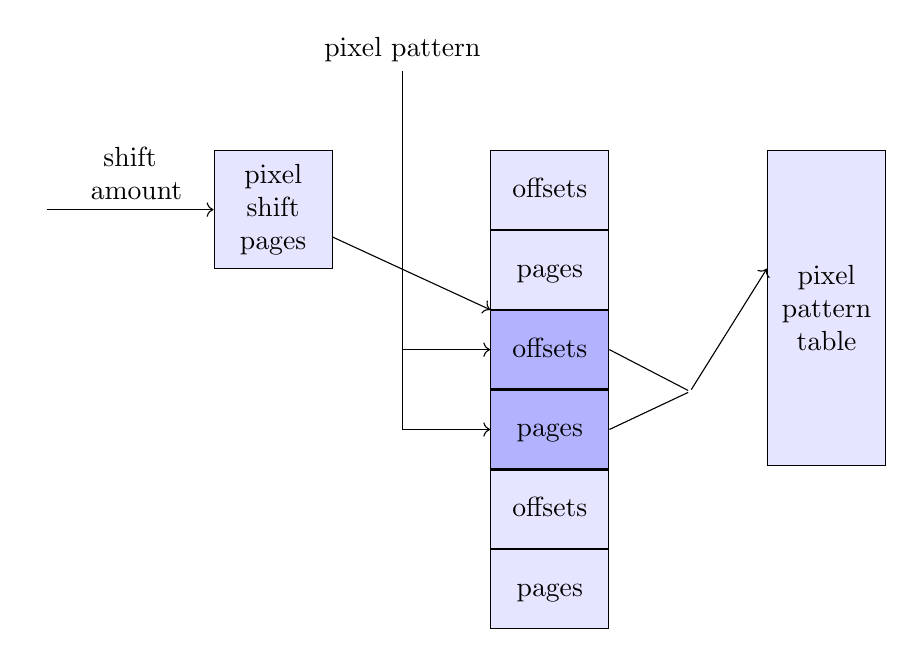
\begin{tikzpicture}
  [basicbox/.style={draw,rectangle,inner sep=0pt,minimum width=1.5cm,minimum height=1.5cm,fill=blue!10},
   pageoffsets/.style={basicbox,minimum height=1cm,text height=1.5ex,text depth=.25ex},
   multilinebox/.style={basicbox,text width=1cm,align=center}]
  \node (pixelshiftpages) at (0,0) [multilinebox] {pixel shift pages};
  \node (start) at (-3,0) {};
  \draw [->] (start) -- (pixelshiftpages) node [above,text width=1cm,align=center,midway] {shift amount};
  \node (offsets0) [pageoffsets,anchor=north,below right=0 and 2 of pixelshiftpages.north east] {offsets};
  \node (pages0) [pageoffsets,below=0 of offsets0.south] {pages};
  \node (offsets1) [pageoffsets,below=0 of pages0.south,fill=blue!30] {offsets};
  \node (pages1) [pageoffsets,below=0 of offsets1.south,fill=blue!30] {pages};
  \node (offsets2) [pageoffsets,below=0 of pages1.south] {offsets};
  \node (pages2) [pageoffsets,below=0 of offsets2.south] {pages};
  \draw [->] (pixelshiftpages) -- (offsets1.north west) {};
  \node (pixelpattern) [above left=1 and 0 of offsets0.north west] {pixel pattern};
  \draw [->] (pixelpattern.south) |- (offsets1.west) {};
  \draw [->] (pixelpattern.south) |- (pages1.west) {};
  \node (patterntable) [multilinebox,minimum height=4cm,text width=1.2cm,anchor=north west,below right=0 and 2 of offsets0.north east] {pixel pattern table};
  \node (join) [inner sep=0pt,below right=0 and 1 of offsets1.south east] {};
  \draw (offsets1.east) -- (join);
  \draw (pages1.east) -- (join);
  \draw [->] (join) -- ([yshift=5mm]patterntable.west);
\end{tikzpicture}
\vspace{1em}

The pixel pattern table is a table of every possible pattern of 7 consecutive pixels
spread out over two bytes. This table is 512 entries, each entry being two bytes.
A naive table would have redundancy. For example the pattern {\Tt{}0000100\nwendquote} starting
at column 0 is exactly the same as the pattern {\Tt{}0001000\nwendquote} starting at column 1.
This table eliminates that redundancy.

\nwenddocs{}\nwbegincode{12}\sublabel{NW1Xx3lK-1W8AJS-2}\nwmargintag{{\nwtagstyle{}\subpageref{NW1Xx3lK-1W8AJS-2}}}\moddef{tables~{\nwtagstyle{}\subpageref{NW1Xx3lK-1W8AJS-1}}}\plusendmoddef\nwstartdeflinemarkup\nwusesondefline{\\{NW1Xx3lK-1p0Y9w-1}}\nwprevnextdefs{NW1Xx3lK-1W8AJS-1}{NW1Xx3lK-1W8AJS-3}\nwenddeflinemarkup
    ORG     $A900
\nwlinkedidentc{PIXEL_PATTERN_TABLE}{NW1Xx3lK-1W8AJS-2}:
    INCLUDE "pixel_pattern_table.asm"
\nwindexdefn{\nwixident{PIXEL{\_}PATTERN{\_}TABLE}}{PIXEL:unPATTERN:unTABLE}{NW1Xx3lK-1W8AJS-2}\eatline
\nwused{\\{NW1Xx3lK-1p0Y9w-1}}\nwidentdefs{\\{{\nwixident{PIXEL{\_}PATTERN{\_}TABLE}}{PIXEL:unPATTERN:unTABLE}}}\nwendcode{}\nwbegindocs{13}\nwdocspar
Now we just need tables which index into {\Tt{}\nwlinkedidentq{PIXEL{\_}PATTERN{\_}TABLE}{NW1Xx3lK-1W8AJS-2}\nwendquote} for every
7-pixel pattern and shift value. This table works by having the page number
for the shifted pixel pattern at index {\Tt{}shift\ *\ 0x100\ +\ 0x80\ +\ pattern\nwendquote}
and the offset at index {\Tt{}shift\ *\ 0x100\ +\ pattern\nwendquote}.

\nwenddocs{}\nwbegincode{14}\sublabel{NW1Xx3lK-1W8AJS-3}\nwmargintag{{\nwtagstyle{}\subpageref{NW1Xx3lK-1W8AJS-3}}}\moddef{tables~{\nwtagstyle{}\subpageref{NW1Xx3lK-1W8AJS-1}}}\plusendmoddef\nwstartdeflinemarkup\nwusesondefline{\\{NW1Xx3lK-1p0Y9w-1}}\nwprevnextdefs{NW1Xx3lK-1W8AJS-2}{NW1Xx3lK-1W8AJS-4}\nwenddeflinemarkup
    ORG     $A200
\nwlinkedidentc{PIXEL_SHIFT_TABLE}{NW1Xx3lK-1W8AJS-3}:
    INCLUDE "pixel_shift_table.asm"
\nwindexdefn{\nwixident{PIXEL{\_}SHIFT{\_}TABLE}}{PIXEL:unSHIFT:unTABLE}{NW1Xx3lK-1W8AJS-3}\eatline
\nwused{\\{NW1Xx3lK-1p0Y9w-1}}\nwidentdefs{\\{{\nwixident{PIXEL{\_}SHIFT{\_}TABLE}}{PIXEL:unSHIFT:unTABLE}}}\nwendcode{}\nwbegindocs{15}\nwdocspar
Rather than multiplying the shift value by {\Tt{}0x100\nwendquote}, we instead define
another table which holds the page numbers for the shift tables for each
shift value.

\nwenddocs{}\nwbegincode{16}\sublabel{NW1Xx3lK-1W8AJS-4}\nwmargintag{{\nwtagstyle{}\subpageref{NW1Xx3lK-1W8AJS-4}}}\moddef{tables~{\nwtagstyle{}\subpageref{NW1Xx3lK-1W8AJS-1}}}\plusendmoddef\nwstartdeflinemarkup\nwusesondefline{\\{NW1Xx3lK-1p0Y9w-1}}\nwprevnextdefs{NW1Xx3lK-1W8AJS-3}{NW1Xx3lK-1W8AJS-5}\nwenddeflinemarkup
    ORG     $84C1
\nwlinkedidentc{PIXEL_SHIFT_PAGES}{NW1Xx3lK-1W8AJS-4}:
    HEX     A2 A3 A4 A5 A6 A7 A8
\nwindexdefn{\nwixident{PIXEL{\_}SHIFT{\_}PAGES}}{PIXEL:unSHIFT:unPAGES}{NW1Xx3lK-1W8AJS-4}\eatline
\nwused{\\{NW1Xx3lK-1p0Y9w-1}}\nwidentdefs{\\{{\nwixident{PIXEL{\_}SHIFT{\_}PAGES}}{PIXEL:unSHIFT:unPAGES}}}\nwendcode{}\nwbegindocs{17}\nwdocspar
So we can get shifted pixels by indexing into all these tables.

Now we can define a routine that will take a sprite number and a pixel shift
amount, and write the shifted pixel data into the {\Tt{}\nwlinkedidentq{BLOCK{\_}DATA}{NW1Xx3lK-10jlgu-3}\nwendquote} area. The
routine first shifts the first byte of the sprite into a two-byte area. Then
it shifts the second byte of the sprite, and combines that two-byte result
with the first. Thus, we shift two bytes of sprite data into a three-byte
result.

\begin{center}
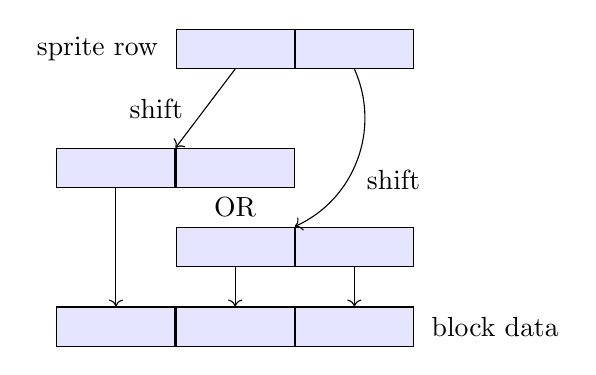
\begin{tikzpicture}
  [basicbox/.style={draw,rectangle,inner sep=0pt,minimum width=1.5cm,minimum height=0.5cm,fill=blue!10}]
  \node (spriterowbyte0) at (0,0) [basicbox] {};
  \node (spriterowbyte1) [basicbox,right=0 of spriterowbyte0.east] {};
  \node (spriterowlabel) [left=0.1 of spriterowbyte0.west] {sprite row};
  \node (shifted0byte0) [basicbox,below left=1 and 0 of spriterowbyte0.south west] {};
  \node (shifted0byte1) [basicbox,right=0 of shifted0byte0.east] {};
  \node (shifted1byte0) [basicbox,below right=2 and 0 of spriterowbyte0.south west] {};
  \node (shifted1byte1) [basicbox,right=0 of shifted1byte0.east] {};
  \node (orlabel) [below=0 of shifted0byte1] {OR};
  \draw [->] (spriterowbyte0.south) -- (shifted0byte0.north east)
    node [left,text width=1cm,align=center,midway] {shift};
  \draw [->] (spriterowbyte1.south) to [auto, bend left=45] node {shift} (shifted1byte0.north east);
  \node (result0) [basicbox,below left=0.5 and 0 of shifted1byte0.south west] {};
  \node (result1) [basicbox,right=0 of result0.east] {};
  \node (result2) [basicbox,right=0 of result1.east] {};
  \draw [->] (shifted0byte0) -- (result0) {};
  \draw [->] (shifted1byte0) -- (result1) {};
  \draw [->] (shifted1byte1) -- (result2) {};
  \node (blocklabel) [right=0.1 of result2.east] {block data};
\end{tikzpicture}
\end{center}

Rather than load addresses from the tables and store them, the routine
modifies its own instructions with those addresses.

\nwenddocs{}\nwbegincode{18}\sublabel{NW1Xx3lK-10jlgu-4}\nwmargintag{{\nwtagstyle{}\subpageref{NW1Xx3lK-10jlgu-4}}}\moddef{defines~{\nwtagstyle{}\subpageref{NW1Xx3lK-10jlgu-1}}}\plusendmoddef\nwstartdeflinemarkup\nwusesondefline{\\{NW1Xx3lK-1p0Y9w-1}}\nwprevnextdefs{NW1Xx3lK-10jlgu-3}{NW1Xx3lK-10jlgu-5}\nwenddeflinemarkup
\nwlinkedidentc{ROW_COUNT}{NW1Xx3lK-10jlgu-4}       EQU     $1D
\nwlinkedidentc{SPRITE_NUM}{NW1Xx3lK-10jlgu-4}      EQU     $1E
\nwindexdefn{\nwixident{ROW{\_}COUNT}}{ROW:unCOUNT}{NW1Xx3lK-10jlgu-4}\nwindexdefn{\nwixident{SPRITE{\_}NUM}}{SPRITE:unNUM}{NW1Xx3lK-10jlgu-4}\eatline
\nwused{\\{NW1Xx3lK-1p0Y9w-1}}\nwidentdefs{\\{{\nwixident{ROW{\_}COUNT}}{ROW:unCOUNT}}\\{{\nwixident{SPRITE{\_}NUM}}{SPRITE:unNUM}}}\nwendcode{}\nwbegindocs{19}\nwdocspar
\nwenddocs{}\nwbegincode{20}\sublabel{NW1Xx3lK-8jv1b-2}\nwmargintag{{\nwtagstyle{}\subpageref{NW1Xx3lK-8jv1b-2}}}\moddef{routines~{\nwtagstyle{}\subpageref{NW1Xx3lK-8jv1b-1}}}\plusendmoddef\nwstartdeflinemarkup\nwusesondefline{\\{NW1Xx3lK-1p0Y9w-1}}\nwprevnextdefs{NW1Xx3lK-8jv1b-1}{NW1Xx3lK-8jv1b-3}\nwenddeflinemarkup
    ORG     $8438
\nwlinkedidentc{COMPUTE_SHIFTED_SPRITE}{NW1Xx3lK-8jv1b-2}:
    SUBROUTINE
    ; Enter routine with X set to pixel shift amount and
    ; \nwlinkedidentc{SPRITE_NUM}{NW1Xx3lK-10jlgu-4} containing the sprite number to read.

.offset_table       EQU $A000               ; Target addresses in read
.page_table         EQU $A080               ; instructions. The only truly
.shift_ptr_byte0    EQU $A000               ; necessary value here is the
.shift_ptr_byte1    EQU $A000               ; 0x80 in .shift_ptr_byte0.

    LDA     #$0B                            ; 11 rows
    STA     \nwlinkedidentc{ROW_COUNT}{NW1Xx3lK-10jlgu-4}
    LDA     #<\nwlinkedidentc{SPRITE_DATA}{NW1Xx3lK-1W8AJS-1}
    STA     \nwlinkedidentc{TMP_PTR}{NW1Xx3lK-10jlgu-1}
    LDA     #>\nwlinkedidentc{SPRITE_DATA}{NW1Xx3lK-1W8AJS-1}
    STA     \nwlinkedidentc{TMP_PTR}{NW1Xx3lK-10jlgu-1}+1                       ; \nwlinkedidentc{TMP_PTR}{NW1Xx3lK-10jlgu-1} = \nwlinkedidentc{SPRITE_DATA}{NW1Xx3lK-1W8AJS-1}
    LDA     \nwlinkedidentc{PIXEL_SHIFT_PAGES}{NW1Xx3lK-1W8AJS-4},X 
    STA     .rd_offset_table + 2
    STA     .rd_page_table + 2
    STA     .rd_offset_table2 + 2
    STA     .rd_page_table2 + 2             ; Fix up pages in lookup instructions
                                            ; based on shift amount (X).

    LDX     #$00                            ; X is the offset into \nwlinkedidentc{BLOCK_DATA}{NW1Xx3lK-10jlgu-3}.

.loop:                                      ; === LOOP === (over all 11 rows)
    LDY     \nwlinkedidentc{SPRITE_NUM}{NW1Xx3lK-10jlgu-4}
    LDA     (\nwlinkedidentc{TMP_PTR}{NW1Xx3lK-10jlgu-1}),Y 
    TAY                                     ; Get sprite pixel data.

.rd_offset_table:
    LDA     .offset_table,Y                 ; Load offset for shift amount.
    STA     .rd_shift_ptr_byte0 + 1
    CLC
    ADC     #$01
    STA     .rd_shift_ptr_byte1 + 1         ; Fix up instruction offsets with it.
.rd_page_table:
    LDA     .page_table,Y                   ; Load page for shift amount.
    STA     .rd_shift_ptr_byte0 + 2
    STA     .rd_shift_ptr_byte1 + 2         ; Fix up instruction page with it.

.rd_shift_ptr_byte0:
    LDA     .shift_ptr_byte0                ; Read shifted pixel data byte 0
    STA     \nwlinkedidentc{BLOCK_DATA}{NW1Xx3lK-10jlgu-3},X                    ; and store in block data byte 0.
.rd_shift_ptr_byte1:
    LDA     .shift_ptr_byte1                ; Read shifted pixel data byte 1
    STA     \nwlinkedidentc{BLOCK_DATA}{NW1Xx3lK-10jlgu-3}+1,X                  ; and store in block data byte 1.

    LDA     \nwlinkedidentc{TMP_PTR}{NW1Xx3lK-10jlgu-1}
    CLC
    ADC     #$68
    STA     \nwlinkedidentc{TMP_PTR}{NW1Xx3lK-10jlgu-1}
    LDA     \nwlinkedidentc{TMP_PTR}{NW1Xx3lK-10jlgu-1}+1
    ADC     #$00
    STA     \nwlinkedidentc{TMP_PTR}{NW1Xx3lK-10jlgu-1}+1                       ; \nwlinkedidentc{TMP_PTR}{NW1Xx3lK-10jlgu-1}++

    ; Now basically do the same thing with the second sprite byte

    LDY     \nwlinkedidentc{SPRITE_NUM}{NW1Xx3lK-10jlgu-4}
    LDA     (\nwlinkedidentc{TMP_PTR}{NW1Xx3lK-10jlgu-1}),Y 
    TAY                                     ; Get sprite pixel data.

.rd_offset_table2:
    LDA     .offset_table,Y                 ; Load offset for shift amount.
    STA     .rd_shift_ptr2_byte0 + 1
    CLC
    ADC     #$01
    STA     .rd_shift_ptr2_byte1 + 1        ; Fix up instruction offsets with it.
.rd_page_table2:
    LDA     .page_table,Y                   ; Load page for shift amount.
    STA     .rd_shift_ptr2_byte0 + 2
    STA     .rd_shift_ptr2_byte1 + 2        ; Fix up instruction page with it.

.rd_shift_ptr2_byte0:
    LDA     .shift_ptr_byte0                ; Read shifted pixel data byte 0
    ORA     \nwlinkedidentc{BLOCK_DATA}{NW1Xx3lK-10jlgu-3}+1,X                  ; OR with previous block data byte 1
    STA     \nwlinkedidentc{BLOCK_DATA}{NW1Xx3lK-10jlgu-3}+1,X                  ; and store in block data byte 1.
.rd_shift_ptr2_byte1:
    LDA     .shift_ptr_byte1                ; Read shifted pixel data byte 1
    STA     \nwlinkedidentc{BLOCK_DATA}{NW1Xx3lK-10jlgu-3}+2,X                  ; and store in block data byte 2.

    LDA     \nwlinkedidentc{TMP_PTR}{NW1Xx3lK-10jlgu-1}
    CLC
    ADC     #$68
    STA     \nwlinkedidentc{TMP_PTR}{NW1Xx3lK-10jlgu-1}
    LDA     \nwlinkedidentc{TMP_PTR}{NW1Xx3lK-10jlgu-1}+1
    ADC     #$00
    STA     \nwlinkedidentc{TMP_PTR}{NW1Xx3lK-10jlgu-1}+1                       ; \nwlinkedidentc{TMP_PTR}{NW1Xx3lK-10jlgu-1}++

    INX
    INX
    INX                                     ; X += 3
    DEC     \nwlinkedidentc{ROW_COUNT}{NW1Xx3lK-10jlgu-4}                       ; \nwlinkedidentc{ROW_COUNT}{NW1Xx3lK-10jlgu-4}--
    BNE     .loop                           ; loop while \nwlinkedidentc{ROW_COUNT}{NW1Xx3lK-10jlgu-4} > 0
    RTS
\nwindexdefn{\nwixident{COMPUTE{\_}SHIFTED{\_}SPRITE}}{COMPUTE:unSHIFTED:unSPRITE}{NW1Xx3lK-8jv1b-2}\eatline
\nwused{\\{NW1Xx3lK-1p0Y9w-1}}\nwidentdefs{\\{{\nwixident{COMPUTE{\_}SHIFTED{\_}SPRITE}}{COMPUTE:unSHIFTED:unSPRITE}}}\nwidentuses{\\{{\nwixident{BLOCK{\_}DATA}}{BLOCK:unDATA}}\\{{\nwixident{PIXEL{\_}SHIFT{\_}PAGES}}{PIXEL:unSHIFT:unPAGES}}\\{{\nwixident{ROW{\_}COUNT}}{ROW:unCOUNT}}\\{{\nwixident{SPRITE{\_}DATA}}{SPRITE:unDATA}}\\{{\nwixident{SPRITE{\_}NUM}}{SPRITE:unNUM}}\\{{\nwixident{TMP{\_}PTR}}{TMP:unPTR}}}\nwindexuse{\nwixident{BLOCK{\_}DATA}}{BLOCK:unDATA}{NW1Xx3lK-8jv1b-2}\nwindexuse{\nwixident{PIXEL{\_}SHIFT{\_}PAGES}}{PIXEL:unSHIFT:unPAGES}{NW1Xx3lK-8jv1b-2}\nwindexuse{\nwixident{ROW{\_}COUNT}}{ROW:unCOUNT}{NW1Xx3lK-8jv1b-2}\nwindexuse{\nwixident{SPRITE{\_}DATA}}{SPRITE:unDATA}{NW1Xx3lK-8jv1b-2}\nwindexuse{\nwixident{SPRITE{\_}NUM}}{SPRITE:unNUM}{NW1Xx3lK-8jv1b-2}\nwindexuse{\nwixident{TMP{\_}PTR}}{TMP:unPTR}{NW1Xx3lK-8jv1b-2}\nwendcode{}\nwbegindocs{21}\nwdocspar
\section{Memory mapped graphics}

Within a screen row, consecutive bytes map to consecutive pixels. However, rows
themselves are not consecutive in memory.

To make it easy to convert a row number from 0 to 191 to a base address, Lode Runner has
a table and a routine to use that table.

\nwenddocs{}\nwbegincode{22}\sublabel{NW1Xx3lK-1W8AJS-5}\nwmargintag{{\nwtagstyle{}\subpageref{NW1Xx3lK-1W8AJS-5}}}\moddef{tables~{\nwtagstyle{}\subpageref{NW1Xx3lK-1W8AJS-1}}}\plusendmoddef\nwstartdeflinemarkup\nwusesondefline{\\{NW1Xx3lK-1p0Y9w-1}}\nwprevnextdefs{NW1Xx3lK-1W8AJS-4}{NW1Xx3lK-1W8AJS-6}\nwenddeflinemarkup
    ORG     $1A85
\nwlinkedidentc{ROW_TO_OFFSET_LO}{NW1Xx3lK-1W8AJS-5}:
    INCLUDE "row_to_offset_lo_table.asm"
\nwlinkedidentc{ROW_TO_OFFSET_HI}{NW1Xx3lK-1W8AJS-5}:
    INCLUDE "row_to_offset_hi_table.asm"
\nwindexdefn{\nwixident{ROW{\_}TO{\_}OFFSET{\_}LO}}{ROW:unTO:unOFFSET:unLO}{NW1Xx3lK-1W8AJS-5}\nwindexdefn{\nwixident{ROW{\_}TO{\_}OFFSET{\_}HI}}{ROW:unTO:unOFFSET:unHI}{NW1Xx3lK-1W8AJS-5}\eatline
\nwused{\\{NW1Xx3lK-1p0Y9w-1}}\nwidentdefs{\\{{\nwixident{ROW{\_}TO{\_}OFFSET{\_}HI}}{ROW:unTO:unOFFSET:unHI}}\\{{\nwixident{ROW{\_}TO{\_}OFFSET{\_}LO}}{ROW:unTO:unOFFSET:unLO}}}\nwendcode{}\nwbegindocs{23}\nwdocspar
\nwenddocs{}\nwbegincode{24}\sublabel{NW1Xx3lK-10jlgu-5}\nwmargintag{{\nwtagstyle{}\subpageref{NW1Xx3lK-10jlgu-5}}}\moddef{defines~{\nwtagstyle{}\subpageref{NW1Xx3lK-10jlgu-1}}}\plusendmoddef\nwstartdeflinemarkup\nwusesondefline{\\{NW1Xx3lK-1p0Y9w-1}}\nwprevnextdefs{NW1Xx3lK-10jlgu-4}{NW1Xx3lK-10jlgu-6}\nwenddeflinemarkup
\nwlinkedidentc{ROW_ADDR}{NW1Xx3lK-10jlgu-5}        EQU     $0C     ; 2 bytes
\nwlinkedidentc{ROW_ADDR2}{NW1Xx3lK-10jlgu-5}       EQU     $0E     ; 2 bytes
\nwlinkedidentc{HGR_PAGE}{NW1Xx3lK-10jlgu-5}        EQU     $1F     ; 0x20 for HGR1, 0x40 for HGR2
\nwindexdefn{\nwixident{ROW{\_}ADDR}}{ROW:unADDR}{NW1Xx3lK-10jlgu-5}\nwindexdefn{\nwixident{ROW{\_}ADDR2}}{ROW:unADDR2}{NW1Xx3lK-10jlgu-5}\nwindexdefn{\nwixident{HGR{\_}PAGE}}{HGR:unPAGE}{NW1Xx3lK-10jlgu-5}\eatline
\nwused{\\{NW1Xx3lK-1p0Y9w-1}}\nwidentdefs{\\{{\nwixident{HGR{\_}PAGE}}{HGR:unPAGE}}\\{{\nwixident{ROW{\_}ADDR}}{ROW:unADDR}}\\{{\nwixident{ROW{\_}ADDR2}}{ROW:unADDR2}}}\nwendcode{}\nwbegindocs{25}\nwdocspar
\nwenddocs{}\nwbegincode{26}\sublabel{NW1Xx3lK-8jv1b-3}\nwmargintag{{\nwtagstyle{}\subpageref{NW1Xx3lK-8jv1b-3}}}\moddef{routines~{\nwtagstyle{}\subpageref{NW1Xx3lK-8jv1b-1}}}\plusendmoddef\nwstartdeflinemarkup\nwusesondefline{\\{NW1Xx3lK-1p0Y9w-1}}\nwprevnextdefs{NW1Xx3lK-8jv1b-2}{NW1Xx3lK-8jv1b-4}\nwenddeflinemarkup
    ORG     $7A31
\nwlinkedidentc{ROW_TO_ADDR}{NW1Xx3lK-8jv1b-3}:
    SUBROUTINE
    ; Enter routine with Y set to row. Base address
    ; (for column 0) will be placed in \nwlinkedidentc{ROW_ADDR}{NW1Xx3lK-10jlgu-5}.

    LDA     \nwlinkedidentc{ROW_TO_OFFSET_LO}{NW1Xx3lK-1W8AJS-5},Y 
    STA     \nwlinkedidentc{ROW_ADDR}{NW1Xx3lK-10jlgu-5}
    LDA     \nwlinkedidentc{ROW_TO_OFFSET_HI}{NW1Xx3lK-1W8AJS-5},Y 
    ORA     \nwlinkedidentc{HGR_PAGE}{NW1Xx3lK-10jlgu-5}
    STA     \nwlinkedidentc{ROW_ADDR}{NW1Xx3lK-10jlgu-5}+1
    RTS
\nwindexdefn{\nwixident{ROW{\_}TO{\_}ADDR}}{ROW:unTO:unADDR}{NW1Xx3lK-8jv1b-3}\eatline
\nwused{\\{NW1Xx3lK-1p0Y9w-1}}\nwidentdefs{\\{{\nwixident{ROW{\_}TO{\_}ADDR}}{ROW:unTO:unADDR}}}\nwidentuses{\\{{\nwixident{HGR{\_}PAGE}}{HGR:unPAGE}}\\{{\nwixident{ROW{\_}ADDR}}{ROW:unADDR}}\\{{\nwixident{ROW{\_}TO{\_}OFFSET{\_}HI}}{ROW:unTO:unOFFSET:unHI}}\\{{\nwixident{ROW{\_}TO{\_}OFFSET{\_}LO}}{ROW:unTO:unOFFSET:unLO}}}\nwindexuse{\nwixident{HGR{\_}PAGE}}{HGR:unPAGE}{NW1Xx3lK-8jv1b-3}\nwindexuse{\nwixident{ROW{\_}ADDR}}{ROW:unADDR}{NW1Xx3lK-8jv1b-3}\nwindexuse{\nwixident{ROW{\_}TO{\_}OFFSET{\_}HI}}{ROW:unTO:unOFFSET:unHI}{NW1Xx3lK-8jv1b-3}\nwindexuse{\nwixident{ROW{\_}TO{\_}OFFSET{\_}LO}}{ROW:unTO:unOFFSET:unLO}{NW1Xx3lK-8jv1b-3}\nwendcode{}\nwbegindocs{27}\nwdocspar
There's also a routine to load the address for both page 1 and page 2.

\nwenddocs{}\nwbegincode{28}\sublabel{NW1Xx3lK-8jv1b-4}\nwmargintag{{\nwtagstyle{}\subpageref{NW1Xx3lK-8jv1b-4}}}\moddef{routines~{\nwtagstyle{}\subpageref{NW1Xx3lK-8jv1b-1}}}\plusendmoddef\nwstartdeflinemarkup\nwusesondefline{\\{NW1Xx3lK-1p0Y9w-1}}\nwprevnextdefs{NW1Xx3lK-8jv1b-3}{NW1Xx3lK-8jv1b-5}\nwenddeflinemarkup
    ORG     $7A3E
\nwlinkedidentc{ROW_TO_ADDR_FOR_BOTH_PAGES}{NW1Xx3lK-8jv1b-4}:
    SUBROUTINE
    ; Enter routine with Y set to row. Base address
    ; (for column 0) will be placed in \nwlinkedidentc{ROW_ADDR}{NW1Xx3lK-10jlgu-5} (for page 1)
    ; and \nwlinkedidentc{ROW_ADDR2}{NW1Xx3lK-10jlgu-5} (for page 2).

    LDA     \nwlinkedidentc{ROW_TO_OFFSET_LO}{NW1Xx3lK-1W8AJS-5},Y 
    STA     \nwlinkedidentc{ROW_ADDR}{NW1Xx3lK-10jlgu-5}
    STA     \nwlinkedidentc{ROW_ADDR2}{NW1Xx3lK-10jlgu-5}
    LDA     \nwlinkedidentc{ROW_TO_OFFSET_HI}{NW1Xx3lK-1W8AJS-5},Y 
    ORA     #$20
    STA     \nwlinkedidentc{ROW_ADDR}{NW1Xx3lK-10jlgu-5}+1
    EOR     #$60
    STA     \nwlinkedidentc{ROW_ADDR2}{NW1Xx3lK-10jlgu-5}+1
    RTS
\nwindexdefn{\nwixident{ROW{\_}TO{\_}ADDR{\_}FOR{\_}BOTH{\_}PAGES}}{ROW:unTO:unADDR:unFOR:unBOTH:unPAGES}{NW1Xx3lK-8jv1b-4}\eatline
\nwused{\\{NW1Xx3lK-1p0Y9w-1}}\nwidentdefs{\\{{\nwixident{ROW{\_}TO{\_}ADDR{\_}FOR{\_}BOTH{\_}PAGES}}{ROW:unTO:unADDR:unFOR:unBOTH:unPAGES}}}\nwidentuses{\\{{\nwixident{ROW{\_}ADDR}}{ROW:unADDR}}\\{{\nwixident{ROW{\_}ADDR2}}{ROW:unADDR2}}\\{{\nwixident{ROW{\_}TO{\_}OFFSET{\_}HI}}{ROW:unTO:unOFFSET:unHI}}\\{{\nwixident{ROW{\_}TO{\_}OFFSET{\_}LO}}{ROW:unTO:unOFFSET:unLO}}}\nwindexuse{\nwixident{ROW{\_}ADDR}}{ROW:unADDR}{NW1Xx3lK-8jv1b-4}\nwindexuse{\nwixident{ROW{\_}ADDR2}}{ROW:unADDR2}{NW1Xx3lK-8jv1b-4}\nwindexuse{\nwixident{ROW{\_}TO{\_}OFFSET{\_}HI}}{ROW:unTO:unOFFSET:unHI}{NW1Xx3lK-8jv1b-4}\nwindexuse{\nwixident{ROW{\_}TO{\_}OFFSET{\_}LO}}{ROW:unTO:unOFFSET:unLO}{NW1Xx3lK-8jv1b-4}\nwendcode{}\nwbegindocs{29}\nwdocspar
Lode Runner's screens are organized into 28 sprites across by 17 sprites
down. To convert between sprite coordinates and screen coordinates and vice-versa, we
use tables and lookup routines. Each sprite is 10 pixels across by 11 pixels down.

Note that the last row is used for the status, so actually the game screen is 16 sprites vertically.

\nwenddocs{}\nwbegincode{30}\sublabel{NW1Xx3lK-10jlgu-6}\nwmargintag{{\nwtagstyle{}\subpageref{NW1Xx3lK-10jlgu-6}}}\moddef{defines~{\nwtagstyle{}\subpageref{NW1Xx3lK-10jlgu-1}}}\plusendmoddef\nwstartdeflinemarkup\nwusesondefline{\\{NW1Xx3lK-1p0Y9w-1}}\nwprevnextdefs{NW1Xx3lK-10jlgu-5}{NW1Xx3lK-10jlgu-7}\nwenddeflinemarkup
MAX_GAME_COL        EQU     #27     ; 0x1B
MAX_GAME_ROW        EQU     #15     ; 0x0F
\nwused{\\{NW1Xx3lK-1p0Y9w-1}}\nwendcode{}\nwbegindocs{31}\nwdocspar

\nwenddocs{}\nwbegincode{32}\sublabel{NW1Xx3lK-1W8AJS-6}\nwmargintag{{\nwtagstyle{}\subpageref{NW1Xx3lK-1W8AJS-6}}}\moddef{tables~{\nwtagstyle{}\subpageref{NW1Xx3lK-1W8AJS-1}}}\plusendmoddef\nwstartdeflinemarkup\nwusesondefline{\\{NW1Xx3lK-1p0Y9w-1}}\nwprevnextdefs{NW1Xx3lK-1W8AJS-5}{NW1Xx3lK-1W8AJS-7}\nwenddeflinemarkup
    ORG     $1C35
\nwlinkedidentc{HALF_SCREEN_COL_TABLE}{NW1Xx3lK-1W8AJS-6}:
    ; 28 cols of 5 double-pixels each
    HEX     00 05 0a 0f 14 19 1e 23 28 2d 32 37 3c 41 46 4b
    HEX     50 55 5a 5f 64 69 6e 73 78 7d 82 87
\nwlinkedidentc{SCREEN_ROW_TABLE}{NW1Xx3lK-1W8AJS-6}:
    ; 17 rows of 11 pixels each
    HEX     00 0B 16 21 2C 37 42 4D 58 63 6E 79 84 8F 9A A5
    HEX     B5
\nwlinkedidentc{COL_BYTE_TABLE}{NW1Xx3lK-1W8AJS-6}:
    ; Byte number
    HEX     00 01 02 04 05 07 08 0A 0B 0C 0E 0F 11 12 14 15
    HEX     16 18 19 1B 1C 1E 1F 20 22 23 25 26
\nwlinkedidentc{COL_SHIFT_TABLE}{NW1Xx3lK-1W8AJS-6}:
    ; Right shift amount
    HEX     00 03 06 02 05 01 04 00 03 06 02 05 01 04 00 03
    HEX     06 02 05 01 04 00 03 06 02 05 01 04
\nwlinkedidentc{HALF_SCREEN_COL_BYTE_TABLE}{NW1Xx3lK-1W8AJS-6}:
    HEX     00 00 00 00 01 01 01 02 02 02 02 03 03 03 04 04
    HEX     04 04 05 05 05 06 06 06 06 07 07 07 08 08 08 08
    HEX     09 09 09 0A 0A 0A 0A 0B 0B 0B 0C 0C 0C 0C 0D 0D
    HEX     0D 0E 0E 0E 0E 0F 0F 0F 10 10 10 10 11 11 11 12
    HEX     12 12 12 13 13 13 14 14 14 14 15 15 15 16 16 16
    HEX     16 17 17 17 18 18 18 18 19 19 19 1A 1A 1A 1A 1B
    HEX     1B 1B 1C 1C 1C 1C 1D 1D 1D 1E 1E 1E 1E 1F 1F 1F
    HEX     20 20 20 20 21 21 21 22 22 22 22 23 23 23 24 24
    HEX     24 24 25 25 25 26 26 26 26 27 27 27
\nwlinkedidentc{HALF_SCREEN_COL_SHIFT_TABLE}{NW1Xx3lK-1W8AJS-6}:
    HEX     00 02 04 06 01 03 05 00 02 04 06 01 03 05 00 02
    HEX     04 06 01 03 05 00 02 04 06 01 03 05 00 02 04 06
    HEX     01 03 05 00 02 04 06 01 03 05 00 02 04 06 01 03
    HEX     05 00 02 04 06 01 03 05 00 02 04 06 01 03 05 00
    HEX     02 04 06 01 03 05 00 02 04 06 01 03 05 00 02 04
    HEX     06 01 03 05 00 02 04 06 01 03 05 00 02 04 06 01
    HEX     03 05 00 02 04 06 01 03 05 00 02 04 06 01 03 05
    HEX     00 02 04 06 01 03 05 00 02 04 06 01 03 05 00 02
    HEX     04 06 01 03 05 00 02 04 06 01 03 05
\nwindexdefn{\nwixident{SCREEN{\_}ROW{\_}TABLE}}{SCREEN:unROW:unTABLE}{NW1Xx3lK-1W8AJS-6}\nwindexdefn{\nwixident{COL{\_}BYTE{\_}TABLE}}{COL:unBYTE:unTABLE}{NW1Xx3lK-1W8AJS-6}\nwindexdefn{\nwixident{HALF{\_}SCREEN{\_}COL{\_}TABLE}}{HALF:unSCREEN:unCOL:unTABLE}{NW1Xx3lK-1W8AJS-6}\nwindexdefn{\nwixident{COL{\_}SHIFT{\_}TABLE}}{COL:unSHIFT:unTABLE}{NW1Xx3lK-1W8AJS-6}\nwindexdefn{\nwixident{HALF{\_}SCREEN{\_}COL{\_}BYTE{\_}TABLE}}{HALF:unSCREEN:unCOL:unBYTE:unTABLE}{NW1Xx3lK-1W8AJS-6}\nwindexdefn{\nwixident{HALF{\_}SCREEN{\_}COL{\_}SHIFT{\_}TABLE}}{HALF:unSCREEN:unCOL:unSHIFT:unTABLE}{NW1Xx3lK-1W8AJS-6}\eatline
\nwused{\\{NW1Xx3lK-1p0Y9w-1}}\nwidentdefs{\\{{\nwixident{COL{\_}BYTE{\_}TABLE}}{COL:unBYTE:unTABLE}}\\{{\nwixident{COL{\_}SHIFT{\_}TABLE}}{COL:unSHIFT:unTABLE}}\\{{\nwixident{HALF{\_}SCREEN{\_}COL{\_}BYTE{\_}TABLE}}{HALF:unSCREEN:unCOL:unBYTE:unTABLE}}\\{{\nwixident{HALF{\_}SCREEN{\_}COL{\_}SHIFT{\_}TABLE}}{HALF:unSCREEN:unCOL:unSHIFT:unTABLE}}\\{{\nwixident{HALF{\_}SCREEN{\_}COL{\_}TABLE}}{HALF:unSCREEN:unCOL:unTABLE}}\\{{\nwixident{SCREEN{\_}ROW{\_}TABLE}}{SCREEN:unROW:unTABLE}}}\nwendcode{}\nwbegindocs{33}\nwdocspar
Here is the routine to return the screen coordinates for the given sprite coordinates.
The reason that {\Tt{}\nwlinkedidentq{GET{\_}SCREEN{\_}COORDS{\_}FOR}{NW1Xx3lK-8jv1b-5}\nwendquote} returns half the screen column coordinate
is that otherwise the screen column coordinate wouldn't fit in a register.

\nwenddocs{}\nwbegincode{34}\sublabel{NW1Xx3lK-8jv1b-5}\nwmargintag{{\nwtagstyle{}\subpageref{NW1Xx3lK-8jv1b-5}}}\moddef{routines~{\nwtagstyle{}\subpageref{NW1Xx3lK-8jv1b-1}}}\plusendmoddef\nwstartdeflinemarkup\nwusesondefline{\\{NW1Xx3lK-1p0Y9w-1}}\nwprevnextdefs{NW1Xx3lK-8jv1b-4}{NW1Xx3lK-8jv1b-6}\nwenddeflinemarkup
    ORG     $885D
\nwlinkedidentc{GET_SCREEN_COORDS_FOR}{NW1Xx3lK-8jv1b-5}:
    SUBROUTINE
    ; Enter routine with Y set to sprite row (0-16) and
    ; X set to sprite column (0-27). On return, Y will be set to
    ; screen row, and X is set to half screen column.

    LDA     \nwlinkedidentc{SCREEN_ROW_TABLE}{NW1Xx3lK-1W8AJS-6},Y 
    PHA
    LDA     \nwlinkedidentc{HALF_SCREEN_COL_TABLE}{NW1Xx3lK-1W8AJS-6},X 
    TAX                         ; X = \nwlinkedidentc{HALF_SCREEN_COL_TABLE}{NW1Xx3lK-1W8AJS-6}[X]
    PLA
    TAY                         ; Y = \nwlinkedidentc{SCREEN_ROW_TABLE}{NW1Xx3lK-1W8AJS-6}[Y]
    RTS
\nwindexdefn{\nwixident{GET{\_}SCREEN{\_}COORDS{\_}FOR}}{GET:unSCREEN:unCOORDS:unFOR}{NW1Xx3lK-8jv1b-5}\eatline
\nwused{\\{NW1Xx3lK-1p0Y9w-1}}\nwidentdefs{\\{{\nwixident{GET{\_}SCREEN{\_}COORDS{\_}FOR}}{GET:unSCREEN:unCOORDS:unFOR}}}\nwidentuses{\\{{\nwixident{HALF{\_}SCREEN{\_}COL{\_}TABLE}}{HALF:unSCREEN:unCOL:unTABLE}}\\{{\nwixident{SCREEN{\_}ROW{\_}TABLE}}{SCREEN:unROW:unTABLE}}}\nwindexuse{\nwixident{HALF{\_}SCREEN{\_}COL{\_}TABLE}}{HALF:unSCREEN:unCOL:unTABLE}{NW1Xx3lK-8jv1b-5}\nwindexuse{\nwixident{SCREEN{\_}ROW{\_}TABLE}}{SCREEN:unROW:unTABLE}{NW1Xx3lK-8jv1b-5}\nwendcode{}\nwbegindocs{35}\nwdocspar
This routine takes a sprite column and converts it to
the memory-mapped byte offset and right-shift amount.

\nwenddocs{}\nwbegincode{36}\sublabel{NW1Xx3lK-8jv1b-6}\nwmargintag{{\nwtagstyle{}\subpageref{NW1Xx3lK-8jv1b-6}}}\moddef{routines~{\nwtagstyle{}\subpageref{NW1Xx3lK-8jv1b-1}}}\plusendmoddef\nwstartdeflinemarkup\nwusesondefline{\\{NW1Xx3lK-1p0Y9w-1}}\nwprevnextdefs{NW1Xx3lK-8jv1b-5}{NW1Xx3lK-8jv1b-7}\nwenddeflinemarkup
    ORG     $8868
\nwlinkedidentc{GET_BYTE_AND_SHIFT_FOR_COL}{NW1Xx3lK-8jv1b-6}:
    SUBROUTINE
    ; Enter routine with X set to sprite column. On
    ; return, A will be set to screen column byte number
    ; and X will be set to an additional right shift amount.

    LDA     \nwlinkedidentc{COL_BYTE_TABLE}{NW1Xx3lK-1W8AJS-6},X 
    PHA                         ; A = \nwlinkedidentc{COL_BYTE_TABLE}{NW1Xx3lK-1W8AJS-6}[X]
    LDA     \nwlinkedidentc{COL_SHIFT_TABLE}{NW1Xx3lK-1W8AJS-6},X 
    TAX                         ; X = \nwlinkedidentc{COL_SHIFT_TABLE}{NW1Xx3lK-1W8AJS-6}[X]
    PLA
    RTS
\nwindexdefn{\nwixident{GET{\_}BYTE{\_}AND{\_}SHIFT{\_}FOR{\_}COL}}{GET:unBYTE:unAND:unSHIFT:unFOR:unCOL}{NW1Xx3lK-8jv1b-6}\eatline
\nwused{\\{NW1Xx3lK-1p0Y9w-1}}\nwidentdefs{\\{{\nwixident{GET{\_}BYTE{\_}AND{\_}SHIFT{\_}FOR{\_}COL}}{GET:unBYTE:unAND:unSHIFT:unFOR:unCOL}}}\nwidentuses{\\{{\nwixident{COL{\_}BYTE{\_}TABLE}}{COL:unBYTE:unTABLE}}\\{{\nwixident{COL{\_}SHIFT{\_}TABLE}}{COL:unSHIFT:unTABLE}}}\nwindexuse{\nwixident{COL{\_}BYTE{\_}TABLE}}{COL:unBYTE:unTABLE}{NW1Xx3lK-8jv1b-6}\nwindexuse{\nwixident{COL{\_}SHIFT{\_}TABLE}}{COL:unSHIFT:unTABLE}{NW1Xx3lK-8jv1b-6}\nwendcode{}\nwbegindocs{37}\nwdocspar
This routine takes half the screen column coordinate and converts it to
the memory-mapped byte offset and right-shift amount.

\nwenddocs{}\nwbegincode{38}\sublabel{NW1Xx3lK-8jv1b-7}\nwmargintag{{\nwtagstyle{}\subpageref{NW1Xx3lK-8jv1b-7}}}\moddef{routines~{\nwtagstyle{}\subpageref{NW1Xx3lK-8jv1b-1}}}\plusendmoddef\nwstartdeflinemarkup\nwusesondefline{\\{NW1Xx3lK-1p0Y9w-1}}\nwprevnextdefs{NW1Xx3lK-8jv1b-6}{NW1Xx3lK-8jv1b-8}\nwenddeflinemarkup
    ORG     $8872
\nwlinkedidentc{GET_BYTE_AND_SHIFT_FOR_HALF_SCREEN_COL}{NW1Xx3lK-8jv1b-7}:
    SUBROUTINE
    ; Enter routine with X set to half screen column. On
    ; return, A will be set to screen column byte number
    ; and X will be set to an additional right shift amount.

    LDA     \nwlinkedidentc{HALF_SCREEN_COL_BYTE_TABLE}{NW1Xx3lK-1W8AJS-6},X 
    PHA                         ; A = \nwlinkedidentc{HALF_SCREEN_COL_BYTE_TABLE}{NW1Xx3lK-1W8AJS-6}[X]
    LDA     \nwlinkedidentc{HALF_SCREEN_COL_SHIFT_TABLE}{NW1Xx3lK-1W8AJS-6},X 
    TAX                         ; X = \nwlinkedidentc{HALF_SCREEN_COL_SHIFT_TABLE}{NW1Xx3lK-1W8AJS-6}[X]
    PLA
    RTS
\nwindexdefn{\nwixident{GET{\_}BYTE{\_}AND{\_}SHIFT{\_}FOR{\_}HALF{\_}SCREEN{\_}COL}}{GET:unBYTE:unAND:unSHIFT:unFOR:unHALF:unSCREEN:unCOL}{NW1Xx3lK-8jv1b-7}\eatline
\nwused{\\{NW1Xx3lK-1p0Y9w-1}}\nwidentdefs{\\{{\nwixident{GET{\_}BYTE{\_}AND{\_}SHIFT{\_}FOR{\_}HALF{\_}SCREEN{\_}COL}}{GET:unBYTE:unAND:unSHIFT:unFOR:unHALF:unSCREEN:unCOL}}}\nwidentuses{\\{{\nwixident{HALF{\_}SCREEN{\_}COL{\_}BYTE{\_}TABLE}}{HALF:unSCREEN:unCOL:unBYTE:unTABLE}}\\{{\nwixident{HALF{\_}SCREEN{\_}COL{\_}SHIFT{\_}TABLE}}{HALF:unSCREEN:unCOL:unSHIFT:unTABLE}}}\nwindexuse{\nwixident{HALF{\_}SCREEN{\_}COL{\_}BYTE{\_}TABLE}}{HALF:unSCREEN:unCOL:unBYTE:unTABLE}{NW1Xx3lK-8jv1b-7}\nwindexuse{\nwixident{HALF{\_}SCREEN{\_}COL{\_}SHIFT{\_}TABLE}}{HALF:unSCREEN:unCOL:unSHIFT:unTABLE}{NW1Xx3lK-8jv1b-7}\nwendcode{}\nwbegindocs{39}\nwdocspar
We also have some utility routines that let us take a sprite row or column and
get its screen row or half column, but offset in either row or column by anywhere from
{\Tt{}-2\nwendquote} to {\Tt{}+2\nwendquote}.

\nwenddocs{}\nwbegincode{40}\sublabel{NW1Xx3lK-1W8AJS-7}\nwmargintag{{\nwtagstyle{}\subpageref{NW1Xx3lK-1W8AJS-7}}}\moddef{tables~{\nwtagstyle{}\subpageref{NW1Xx3lK-1W8AJS-1}}}\plusendmoddef\nwstartdeflinemarkup\nwusesondefline{\\{NW1Xx3lK-1p0Y9w-1}}\nwprevnextdefs{NW1Xx3lK-1W8AJS-6}{NW1Xx3lK-1W8AJS-8}\nwenddeflinemarkup
    ORG     $888A
\nwlinkedidentc{ROW_OFFSET_TABLE}{NW1Xx3lK-1W8AJS-7}:
    HEX     FB FD 00 02 04
\nwindexdefn{\nwixident{ROW{\_}OFFSET{\_}TABLE}}{ROW:unOFFSET:unTABLE}{NW1Xx3lK-1W8AJS-7}\eatline
\nwused{\\{NW1Xx3lK-1p0Y9w-1}}\nwidentdefs{\\{{\nwixident{ROW{\_}OFFSET{\_}TABLE}}{ROW:unOFFSET:unTABLE}}}\nwendcode{}\nwbegindocs{41}\nwdocspar
\nwenddocs{}\nwbegincode{42}\sublabel{NW1Xx3lK-8jv1b-8}\nwmargintag{{\nwtagstyle{}\subpageref{NW1Xx3lK-8jv1b-8}}}\moddef{routines~{\nwtagstyle{}\subpageref{NW1Xx3lK-8jv1b-1}}}\plusendmoddef\nwstartdeflinemarkup\nwusesondefline{\\{NW1Xx3lK-1p0Y9w-1}}\nwprevnextdefs{NW1Xx3lK-8jv1b-7}{NW1Xx3lK-8jv1b-9}\nwenddeflinemarkup
    ORG     $887C
\nwlinkedidentc{GET_SCREEN_ROW_OFFSET_IN_X_FOR}{NW1Xx3lK-8jv1b-8}:
    SUBROUTINE
    ; Enter routine with X set to offset+2 (in double-pixels) and
    ; Y set to sprite row. On return, X will retain its value and
    ; Y will be set to the screen row.

    TXA
    PHA
    JSR     \nwlinkedidentc{GET_SCREEN_COORDS_FOR}{NW1Xx3lK-8jv1b-5}
    PLA
    TAX                                 ; Restore X
    TYA
    CLC
    ADC     \nwlinkedidentc{ROW_OFFSET_TABLE}{NW1Xx3lK-1W8AJS-7},X
    TAY
    RTS
\nwindexdefn{\nwixident{GET{\_}SCREEN{\_}ROW{\_}OFFSET{\_}IN{\_}X{\_}FOR}}{GET:unSCREEN:unROW:unOFFSET:unIN:unX:unFOR}{NW1Xx3lK-8jv1b-8}\eatline
\nwused{\\{NW1Xx3lK-1p0Y9w-1}}\nwidentdefs{\\{{\nwixident{GET{\_}SCREEN{\_}ROW{\_}OFFSET{\_}IN{\_}X{\_}FOR}}{GET:unSCREEN:unROW:unOFFSET:unIN:unX:unFOR}}}\nwidentuses{\\{{\nwixident{GET{\_}SCREEN{\_}COORDS{\_}FOR}}{GET:unSCREEN:unCOORDS:unFOR}}\\{{\nwixident{ROW{\_}OFFSET{\_}TABLE}}{ROW:unOFFSET:unTABLE}}}\nwindexuse{\nwixident{GET{\_}SCREEN{\_}COORDS{\_}FOR}}{GET:unSCREEN:unCOORDS:unFOR}{NW1Xx3lK-8jv1b-8}\nwindexuse{\nwixident{ROW{\_}OFFSET{\_}TABLE}}{ROW:unOFFSET:unTABLE}{NW1Xx3lK-8jv1b-8}\nwendcode{}\nwbegindocs{43}\nwdocspar
\nwenddocs{}\nwbegincode{44}\sublabel{NW1Xx3lK-1W8AJS-8}\nwmargintag{{\nwtagstyle{}\subpageref{NW1Xx3lK-1W8AJS-8}}}\moddef{tables~{\nwtagstyle{}\subpageref{NW1Xx3lK-1W8AJS-1}}}\plusendmoddef\nwstartdeflinemarkup\nwusesondefline{\\{NW1Xx3lK-1p0Y9w-1}}\nwprevnextdefs{NW1Xx3lK-1W8AJS-7}{NW1Xx3lK-1W8AJS-9}\nwenddeflinemarkup
    ORG     $889D
\nwlinkedidentc{COL_OFFSET_TABLE}{NW1Xx3lK-1W8AJS-8}:
    HEX     FE FF 00 01 02
\nwindexdefn{\nwixident{COL{\_}OFFSET{\_}TABLE}}{COL:unOFFSET:unTABLE}{NW1Xx3lK-1W8AJS-8}\eatline
\nwused{\\{NW1Xx3lK-1p0Y9w-1}}\nwidentdefs{\\{{\nwixident{COL{\_}OFFSET{\_}TABLE}}{COL:unOFFSET:unTABLE}}}\nwendcode{}\nwbegindocs{45}\nwdocspar
\nwenddocs{}\nwbegincode{46}\sublabel{NW1Xx3lK-8jv1b-9}\nwmargintag{{\nwtagstyle{}\subpageref{NW1Xx3lK-8jv1b-9}}}\moddef{routines~{\nwtagstyle{}\subpageref{NW1Xx3lK-8jv1b-1}}}\plusendmoddef\nwstartdeflinemarkup\nwusesondefline{\\{NW1Xx3lK-1p0Y9w-1}}\nwprevnextdefs{NW1Xx3lK-8jv1b-8}{NW1Xx3lK-8jv1b-A}\nwenddeflinemarkup
    ORG     $888F
\nwlinkedidentc{GET_HALF_SCREEN_COL_OFFSET_IN_Y_FOR}{NW1Xx3lK-8jv1b-9}:
    SUBROUTINE
    ; Enter routine with Y set to offset+2 (in double-pixels) and
    ; X set to sprite column. On return, Y will retain its value and
    ; X will be set to the half screen column.

    TYA
    PHA
    JSR     \nwlinkedidentc{GET_SCREEN_COORDS_FOR}{NW1Xx3lK-8jv1b-5}
    PLA
    TAY                                 ; Restore Y
    TXA
    CLC
    ADC     \nwlinkedidentc{COL_OFFSET_TABLE}{NW1Xx3lK-1W8AJS-8},Y
    TAX
    RTS
\nwindexdefn{\nwixident{GET{\_}HALF{\_}SCREEN{\_}COL{\_}OFFSET{\_}IN{\_}Y{\_}FOR}}{GET:unHALF:unSCREEN:unCOL:unOFFSET:unIN:unY:unFOR}{NW1Xx3lK-8jv1b-9}\eatline
\nwused{\\{NW1Xx3lK-1p0Y9w-1}}\nwidentdefs{\\{{\nwixident{GET{\_}HALF{\_}SCREEN{\_}COL{\_}OFFSET{\_}IN{\_}Y{\_}FOR}}{GET:unHALF:unSCREEN:unCOL:unOFFSET:unIN:unY:unFOR}}}\nwidentuses{\\{{\nwixident{COL{\_}OFFSET{\_}TABLE}}{COL:unOFFSET:unTABLE}}\\{{\nwixident{GET{\_}SCREEN{\_}COORDS{\_}FOR}}{GET:unSCREEN:unCOORDS:unFOR}}}\nwindexuse{\nwixident{COL{\_}OFFSET{\_}TABLE}}{COL:unOFFSET:unTABLE}{NW1Xx3lK-8jv1b-9}\nwindexuse{\nwixident{GET{\_}SCREEN{\_}COORDS{\_}FOR}}{GET:unSCREEN:unCOORDS:unFOR}{NW1Xx3lK-8jv1b-9}\nwendcode{}\nwbegindocs{47}\nwdocspar
Now we can finally write the routines that draw a sprite on the screen. We have one
routine that draws a sprite at a given game row and game column.
There are two entry points, one to draw on HGR1, and one for HGR2.

\nwenddocs{}\nwbegincode{48}\sublabel{NW1Xx3lK-10jlgu-7}\nwmargintag{{\nwtagstyle{}\subpageref{NW1Xx3lK-10jlgu-7}}}\moddef{defines~{\nwtagstyle{}\subpageref{NW1Xx3lK-10jlgu-1}}}\plusendmoddef\nwstartdeflinemarkup\nwusesondefline{\\{NW1Xx3lK-1p0Y9w-1}}\nwprevnextdefs{NW1Xx3lK-10jlgu-6}{NW1Xx3lK-10jlgu-8}\nwenddeflinemarkup
\nwlinkedidentc{ROWNUM}{NW1Xx3lK-10jlgu-7}          EQU     $1B
\nwlinkedidentc{COLNUM}{NW1Xx3lK-10jlgu-7}          EQU     $1C
\nwlinkedidentc{MASK0}{NW1Xx3lK-10jlgu-7}           EQU     $50
\nwlinkedidentc{MASK1}{NW1Xx3lK-10jlgu-7}           EQU     $51
\nwlinkedidentc{COL_SHIFT_AMT}{NW1Xx3lK-10jlgu-7}   EQU     $71
\nwlinkedidentc{GAME_COLNUM}{NW1Xx3lK-10jlgu-7}     EQU     $85
\nwlinkedidentc{GAME_ROWNUM}{NW1Xx3lK-10jlgu-7}     EQU     $86
\nwindexdefn{\nwixident{ROWNUM}}{ROWNUM}{NW1Xx3lK-10jlgu-7}\nwindexdefn{\nwixident{COLNUM}}{COLNUM}{NW1Xx3lK-10jlgu-7}\nwindexdefn{\nwixident{MASK0}}{MASK0}{NW1Xx3lK-10jlgu-7}\nwindexdefn{\nwixident{MASK1}}{MASK1}{NW1Xx3lK-10jlgu-7}\nwindexdefn{\nwixident{COL{\_}SHIFT{\_}AMT}}{COL:unSHIFT:unAMT}{NW1Xx3lK-10jlgu-7}\nwindexdefn{\nwixident{GAME{\_}COLNUM}}{GAME:unCOLNUM}{NW1Xx3lK-10jlgu-7}\nwindexdefn{\nwixident{GAME{\_}ROWNUM}}{GAME:unROWNUM}{NW1Xx3lK-10jlgu-7}\eatline
\nwused{\\{NW1Xx3lK-1p0Y9w-1}}\nwidentdefs{\\{{\nwixident{COL{\_}SHIFT{\_}AMT}}{COL:unSHIFT:unAMT}}\\{{\nwixident{COLNUM}}{COLNUM}}\\{{\nwixident{GAME{\_}COLNUM}}{GAME:unCOLNUM}}\\{{\nwixident{GAME{\_}ROWNUM}}{GAME:unROWNUM}}\\{{\nwixident{MASK0}}{MASK0}}\\{{\nwixident{MASK1}}{MASK1}}\\{{\nwixident{ROWNUM}}{ROWNUM}}}\nwendcode{}\nwbegindocs{49}\nwdocspar
\nwenddocs{}\nwbegincode{50}\sublabel{NW1Xx3lK-1W8AJS-9}\nwmargintag{{\nwtagstyle{}\subpageref{NW1Xx3lK-1W8AJS-9}}}\moddef{tables~{\nwtagstyle{}\subpageref{NW1Xx3lK-1W8AJS-1}}}\plusendmoddef\nwstartdeflinemarkup\nwusesondefline{\\{NW1Xx3lK-1p0Y9w-1}}\nwprevnextdefs{NW1Xx3lK-1W8AJS-8}{NW1Xx3lK-1W8AJS-A}\nwenddeflinemarkup
    ORG     $8328
\nwlinkedidentc{PIXEL_MASK0}{NW1Xx3lK-1W8AJS-9}:
    BYTE    %00000000
    BYTE    %00000001
    BYTE    %00000011
    BYTE    %00000111
    BYTE    %00001111
    BYTE    %00011111
    BYTE    %00111111
\nwlinkedidentc{PIXEL_MASK1}{NW1Xx3lK-1W8AJS-9}:
    BYTE    %11111000
    BYTE    %11110000
    BYTE    %11100000
    BYTE    %11000000
    BYTE    %10000000
    BYTE    %11111110
    BYTE    %11111100
\nwindexdefn{\nwixident{PIXEL{\_}MASK0}}{PIXEL:unMASK0}{NW1Xx3lK-1W8AJS-9}\nwindexdefn{\nwixident{PIXEL{\_}MASK1}}{PIXEL:unMASK1}{NW1Xx3lK-1W8AJS-9}\eatline
\nwused{\\{NW1Xx3lK-1p0Y9w-1}}\nwidentdefs{\\{{\nwixident{PIXEL{\_}MASK0}}{PIXEL:unMASK0}}\\{{\nwixident{PIXEL{\_}MASK1}}{PIXEL:unMASK1}}}\nwendcode{}\nwbegindocs{51}\nwdocspar
\nwenddocs{}\nwbegincode{52}\sublabel{NW1Xx3lK-8jv1b-A}\nwmargintag{{\nwtagstyle{}\subpageref{NW1Xx3lK-8jv1b-A}}}\moddef{routines~{\nwtagstyle{}\subpageref{NW1Xx3lK-8jv1b-1}}}\plusendmoddef\nwstartdeflinemarkup\nwusesondefline{\\{NW1Xx3lK-1p0Y9w-1}}\nwprevnextdefs{NW1Xx3lK-8jv1b-9}{NW1Xx3lK-8jv1b-B}\nwenddeflinemarkup
    ORG     $82AA
\nwlinkedidentc{DRAW_SPRITE_PAGE1}{NW1Xx3lK-8jv1b-A}:
    SUBROUTINE
    ; Enter routine with A set to sprite number to draw,
    ; \nwlinkedidentc{GAME_ROWNUM}{NW1Xx3lK-10jlgu-7} set to the row to draw it at, and \nwlinkedidentc{GAME_COLNUM}{NW1Xx3lK-10jlgu-7}
    ; set to the column to draw it at.

    STA     \nwlinkedidentc{SPRITE_NUM}{NW1Xx3lK-10jlgu-4}
    LDA     #$20                ; Page number for HGR1
    BNE     DRAW_SPRITE         ; Actually unconditional jump

\nwlinkedidentc{DRAW_SPRITE_PAGE2}{NW1Xx3lK-8jv1b-A}:
    SUBROUTINE
    ; Enter routine with A set to sprite number to draw,
    ; \nwlinkedidentc{GAME_ROWNUM}{NW1Xx3lK-10jlgu-7} set to the row to draw it at, and \nwlinkedidentc{GAME_COLNUM}{NW1Xx3lK-10jlgu-7}
    ; set to the column to draw it at.

    STA     \nwlinkedidentc{SPRITE_NUM}{NW1Xx3lK-10jlgu-4}
    LDA     #$40                ; Page number for HGR2
    ; fallthrough

DRAW_SPRITE:
    STA     \nwlinkedidentc{HGR_PAGE}{NW1Xx3lK-10jlgu-5}
    LDY     \nwlinkedidentc{GAME_ROWNUM}{NW1Xx3lK-10jlgu-7}
    JSR     \nwlinkedidentc{GET_SCREEN_COORDS_FOR}{NW1Xx3lK-8jv1b-5}
    STY     \nwlinkedidentc{ROWNUM}{NW1Xx3lK-10jlgu-7}              ; \nwlinkedidentc{ROWNUM}{NW1Xx3lK-10jlgu-7} = \nwlinkedidentc{SCREEN_ROW_TABLE}{NW1Xx3lK-1W8AJS-6}[\nwlinkedidentc{GAME_ROWNUM}{NW1Xx3lK-10jlgu-7}]

    LDX     \nwlinkedidentc{GAME_COLNUM}{NW1Xx3lK-10jlgu-7}
    JSR     \nwlinkedidentc{GET_BYTE_AND_SHIFT_FOR_COL}{NW1Xx3lK-8jv1b-6}
    STA     \nwlinkedidentc{COLNUM}{NW1Xx3lK-10jlgu-7}              ; \nwlinkedidentc{COLNUM}{NW1Xx3lK-10jlgu-7} = \nwlinkedidentc{COL_BYTE_TABLE}{NW1Xx3lK-1W8AJS-6}[\nwlinkedidentc{GAME_COLNUM}{NW1Xx3lK-10jlgu-7}]
    STX     \nwlinkedidentc{COL_SHIFT_AMT}{NW1Xx3lK-10jlgu-7}       ; \nwlinkedidentc{COL_SHIFT_AMT}{NW1Xx3lK-10jlgu-7} = \nwlinkedidentc{COL_SHIFT_TABLE}{NW1Xx3lK-1W8AJS-6}[\nwlinkedidentc{GAME_COLNUM}{NW1Xx3lK-10jlgu-7}]

    LDA     \nwlinkedidentc{PIXEL_MASK0}{NW1Xx3lK-1W8AJS-9},X 
    STA     \nwlinkedidentc{MASK0}{NW1Xx3lK-10jlgu-7}               ; \nwlinkedidentc{MASK0}{NW1Xx3lK-10jlgu-7} = \nwlinkedidentc{PIXEL_MASK0}{NW1Xx3lK-1W8AJS-9}[\nwlinkedidentc{COL_SHIFT_AMT}{NW1Xx3lK-10jlgu-7}]
    LDA     \nwlinkedidentc{PIXEL_MASK1}{NW1Xx3lK-1W8AJS-9},X 
    STA     \nwlinkedidentc{MASK1}{NW1Xx3lK-10jlgu-7}               ; \nwlinkedidentc{MASK1}{NW1Xx3lK-10jlgu-7} = \nwlinkedidentc{PIXEL_MASK1}{NW1Xx3lK-1W8AJS-9}[\nwlinkedidentc{COL_SHIFT_AMT}{NW1Xx3lK-10jlgu-7}]

    JSR     \nwlinkedidentc{COMPUTE_SHIFTED_SPRITE}{NW1Xx3lK-8jv1b-2}

    LDA     #$0B
    STA     \nwlinkedidentc{ROW_COUNT}{NW1Xx3lK-10jlgu-4}
    LDX     #$00
    LDA     \nwlinkedidentc{COL_SHIFT_AMT}{NW1Xx3lK-10jlgu-7}
    CMP     #$05
    BCS     .need_3_bytes       ; If \nwlinkedidentc{COL_SHIFT_AMT}{NW1Xx3lK-10jlgu-7} >= 5, we need to alter three
                                ; screen bytes, otherwise just two bytes.

.loop1:
    LDY     \nwlinkedidentc{ROWNUM}{NW1Xx3lK-10jlgu-7}
    JSR     \nwlinkedidentc{ROW_TO_ADDR}{NW1Xx3lK-8jv1b-3}
    LDY     \nwlinkedidentc{COLNUM}{NW1Xx3lK-10jlgu-7}
    LDA     (\nwlinkedidentc{ROW_ADDR}{NW1Xx3lK-10jlgu-5}),Y 
    AND     \nwlinkedidentc{MASK0}{NW1Xx3lK-10jlgu-7}
    ORA     \nwlinkedidentc{BLOCK_DATA}{NW1Xx3lK-10jlgu-3},X 
    STA     (\nwlinkedidentc{ROW_ADDR}{NW1Xx3lK-10jlgu-5}),Y        ; screen[\nwlinkedidentc{COLNUM}{NW1Xx3lK-10jlgu-7}] =
                                ;   screen[\nwlinkedidentc{COLNUM}{NW1Xx3lK-10jlgu-7}] & \nwlinkedidentc{MASK0}{NW1Xx3lK-10jlgu-7} | \nwlinkedidentc{BLOCK_DATA}{NW1Xx3lK-10jlgu-3}[i]

    INX                         ; X++
    INY                         ; Y++
    LDA     (\nwlinkedidentc{ROW_ADDR}{NW1Xx3lK-10jlgu-5}),Y 
    AND     \nwlinkedidentc{MASK1}{NW1Xx3lK-10jlgu-7}
    ORA     \nwlinkedidentc{BLOCK_DATA}{NW1Xx3lK-10jlgu-3},X 
    STA     (\nwlinkedidentc{ROW_ADDR}{NW1Xx3lK-10jlgu-5}),Y        ; screen[\nwlinkedidentc{COLNUM}{NW1Xx3lK-10jlgu-7}+1] =
                                ;   screen[\nwlinkedidentc{COLNUM}{NW1Xx3lK-10jlgu-7}+1] & \nwlinkedidentc{MASK1}{NW1Xx3lK-10jlgu-7} | \nwlinkedidentc{BLOCK_DATA}{NW1Xx3lK-10jlgu-3}[i+1]

    INX
    INX                         ; X += 2
    INC     \nwlinkedidentc{ROWNUM}{NW1Xx3lK-10jlgu-7}              ; \nwlinkedidentc{ROWNUM}{NW1Xx3lK-10jlgu-7}++
    DEC     \nwlinkedidentc{ROW_COUNT}{NW1Xx3lK-10jlgu-4}           ; \nwlinkedidentc{ROW_COUNT}{NW1Xx3lK-10jlgu-4}--
    BNE     .loop1              ; loop while \nwlinkedidentc{ROW_COUNT}{NW1Xx3lK-10jlgu-4} > 0
    RTS

.need_3_bytes
    LDY     \nwlinkedidentc{ROWNUM}{NW1Xx3lK-10jlgu-7}
    JSR     \nwlinkedidentc{ROW_TO_ADDR}{NW1Xx3lK-8jv1b-3}
    LDY     \nwlinkedidentc{COLNUM}{NW1Xx3lK-10jlgu-7}
    LDA     (\nwlinkedidentc{ROW_ADDR}{NW1Xx3lK-10jlgu-5}),Y 
    AND     \nwlinkedidentc{MASK0}{NW1Xx3lK-10jlgu-7}
    ORA     \nwlinkedidentc{BLOCK_DATA}{NW1Xx3lK-10jlgu-3},X 
    STA     (\nwlinkedidentc{ROW_ADDR}{NW1Xx3lK-10jlgu-5}),Y        ; screen[\nwlinkedidentc{COLNUM}{NW1Xx3lK-10jlgu-7}] =
                                ;   screen[\nwlinkedidentc{COLNUM}{NW1Xx3lK-10jlgu-7}] & \nwlinkedidentc{MASK0}{NW1Xx3lK-10jlgu-7} | \nwlinkedidentc{BLOCK_DATA}{NW1Xx3lK-10jlgu-3}[i]

    INX                         ; X++
    INY                         ; Y++
    LDA     \nwlinkedidentc{BLOCK_DATA}{NW1Xx3lK-10jlgu-3},X 
    STA     (\nwlinkedidentc{ROW_ADDR}{NW1Xx3lK-10jlgu-5}),Y        ; screen[\nwlinkedidentc{COLNUM}{NW1Xx3lK-10jlgu-7}+1] = \nwlinkedidentc{BLOCK_DATA}{NW1Xx3lK-10jlgu-3}[i+1]

    INX                         ; X++
    INY                         ; Y++
    LDA     (\nwlinkedidentc{ROW_ADDR}{NW1Xx3lK-10jlgu-5}),Y 
    AND     \nwlinkedidentc{MASK1}{NW1Xx3lK-10jlgu-7}
    ORA     \nwlinkedidentc{BLOCK_DATA}{NW1Xx3lK-10jlgu-3},X 
    STA     (\nwlinkedidentc{ROW_ADDR}{NW1Xx3lK-10jlgu-5}),Y        ; screen[\nwlinkedidentc{COLNUM}{NW1Xx3lK-10jlgu-7}+2] =
                                ;   screen[\nwlinkedidentc{COLNUM}{NW1Xx3lK-10jlgu-7}+2] & \nwlinkedidentc{MASK1}{NW1Xx3lK-10jlgu-7} | \nwlinkedidentc{BLOCK_DATA}{NW1Xx3lK-10jlgu-3}[i+2]

    INX                         ; X++
    INC     \nwlinkedidentc{ROWNUM}{NW1Xx3lK-10jlgu-7}              ; \nwlinkedidentc{ROWNUM}{NW1Xx3lK-10jlgu-7}++
    DEC     \nwlinkedidentc{ROW_COUNT}{NW1Xx3lK-10jlgu-4}           ; \nwlinkedidentc{ROW_COUNT}{NW1Xx3lK-10jlgu-4}--
    BNE     .need_3_bytes       ; loop while \nwlinkedidentc{ROW_COUNT}{NW1Xx3lK-10jlgu-4} > 0
    RTS
\nwindexdefn{\nwixident{DRAW{\_}SPRITE{\_}PAGE1}}{DRAW:unSPRITE:unPAGE1}{NW1Xx3lK-8jv1b-A}\nwindexdefn{\nwixident{DRAW{\_}SPRITE{\_}PAGE2}}{DRAW:unSPRITE:unPAGE2}{NW1Xx3lK-8jv1b-A}\eatline
\nwused{\\{NW1Xx3lK-1p0Y9w-1}}\nwidentdefs{\\{{\nwixident{DRAW{\_}SPRITE{\_}PAGE1}}{DRAW:unSPRITE:unPAGE1}}\\{{\nwixident{DRAW{\_}SPRITE{\_}PAGE2}}{DRAW:unSPRITE:unPAGE2}}}\nwidentuses{\\{{\nwixident{BLOCK{\_}DATA}}{BLOCK:unDATA}}\\{{\nwixident{COL{\_}BYTE{\_}TABLE}}{COL:unBYTE:unTABLE}}\\{{\nwixident{COL{\_}SHIFT{\_}AMT}}{COL:unSHIFT:unAMT}}\\{{\nwixident{COL{\_}SHIFT{\_}TABLE}}{COL:unSHIFT:unTABLE}}\\{{\nwixident{COLNUM}}{COLNUM}}\\{{\nwixident{COMPUTE{\_}SHIFTED{\_}SPRITE}}{COMPUTE:unSHIFTED:unSPRITE}}\\{{\nwixident{GAME{\_}COLNUM}}{GAME:unCOLNUM}}\\{{\nwixident{GAME{\_}ROWNUM}}{GAME:unROWNUM}}\\{{\nwixident{GET{\_}BYTE{\_}AND{\_}SHIFT{\_}FOR{\_}COL}}{GET:unBYTE:unAND:unSHIFT:unFOR:unCOL}}\\{{\nwixident{GET{\_}SCREEN{\_}COORDS{\_}FOR}}{GET:unSCREEN:unCOORDS:unFOR}}\\{{\nwixident{HGR{\_}PAGE}}{HGR:unPAGE}}\\{{\nwixident{MASK0}}{MASK0}}\\{{\nwixident{MASK1}}{MASK1}}\\{{\nwixident{PIXEL{\_}MASK0}}{PIXEL:unMASK0}}\\{{\nwixident{PIXEL{\_}MASK1}}{PIXEL:unMASK1}}\\{{\nwixident{ROW{\_}ADDR}}{ROW:unADDR}}\\{{\nwixident{ROW{\_}COUNT}}{ROW:unCOUNT}}\\{{\nwixident{ROW{\_}TO{\_}ADDR}}{ROW:unTO:unADDR}}\\{{\nwixident{ROWNUM}}{ROWNUM}}\\{{\nwixident{SCREEN{\_}ROW{\_}TABLE}}{SCREEN:unROW:unTABLE}}\\{{\nwixident{SPRITE{\_}NUM}}{SPRITE:unNUM}}}\nwindexuse{\nwixident{BLOCK{\_}DATA}}{BLOCK:unDATA}{NW1Xx3lK-8jv1b-A}\nwindexuse{\nwixident{COL{\_}BYTE{\_}TABLE}}{COL:unBYTE:unTABLE}{NW1Xx3lK-8jv1b-A}\nwindexuse{\nwixident{COL{\_}SHIFT{\_}AMT}}{COL:unSHIFT:unAMT}{NW1Xx3lK-8jv1b-A}\nwindexuse{\nwixident{COL{\_}SHIFT{\_}TABLE}}{COL:unSHIFT:unTABLE}{NW1Xx3lK-8jv1b-A}\nwindexuse{\nwixident{COLNUM}}{COLNUM}{NW1Xx3lK-8jv1b-A}\nwindexuse{\nwixident{COMPUTE{\_}SHIFTED{\_}SPRITE}}{COMPUTE:unSHIFTED:unSPRITE}{NW1Xx3lK-8jv1b-A}\nwindexuse{\nwixident{GAME{\_}COLNUM}}{GAME:unCOLNUM}{NW1Xx3lK-8jv1b-A}\nwindexuse{\nwixident{GAME{\_}ROWNUM}}{GAME:unROWNUM}{NW1Xx3lK-8jv1b-A}\nwindexuse{\nwixident{GET{\_}BYTE{\_}AND{\_}SHIFT{\_}FOR{\_}COL}}{GET:unBYTE:unAND:unSHIFT:unFOR:unCOL}{NW1Xx3lK-8jv1b-A}\nwindexuse{\nwixident{GET{\_}SCREEN{\_}COORDS{\_}FOR}}{GET:unSCREEN:unCOORDS:unFOR}{NW1Xx3lK-8jv1b-A}\nwindexuse{\nwixident{HGR{\_}PAGE}}{HGR:unPAGE}{NW1Xx3lK-8jv1b-A}\nwindexuse{\nwixident{MASK0}}{MASK0}{NW1Xx3lK-8jv1b-A}\nwindexuse{\nwixident{MASK1}}{MASK1}{NW1Xx3lK-8jv1b-A}\nwindexuse{\nwixident{PIXEL{\_}MASK0}}{PIXEL:unMASK0}{NW1Xx3lK-8jv1b-A}\nwindexuse{\nwixident{PIXEL{\_}MASK1}}{PIXEL:unMASK1}{NW1Xx3lK-8jv1b-A}\nwindexuse{\nwixident{ROW{\_}ADDR}}{ROW:unADDR}{NW1Xx3lK-8jv1b-A}\nwindexuse{\nwixident{ROW{\_}COUNT}}{ROW:unCOUNT}{NW1Xx3lK-8jv1b-A}\nwindexuse{\nwixident{ROW{\_}TO{\_}ADDR}}{ROW:unTO:unADDR}{NW1Xx3lK-8jv1b-A}\nwindexuse{\nwixident{ROWNUM}}{ROWNUM}{NW1Xx3lK-8jv1b-A}\nwindexuse{\nwixident{SCREEN{\_}ROW{\_}TABLE}}{SCREEN:unROW:unTABLE}{NW1Xx3lK-8jv1b-A}\nwindexuse{\nwixident{SPRITE{\_}NUM}}{SPRITE:unNUM}{NW1Xx3lK-8jv1b-A}\nwendcode{}\nwbegindocs{53}\nwdocspar
There is a different routine which erases a sprite at a given screen coordinate.
It does this by drawing the inverse of the sprite on page 1, then drawing the sprite data
from page 2 (the background page) onto page 1.

Upon entry, the Y register needs to be set to the screen row coordinate (0-191). However, the
X register needs to be set to half the screen column coordinate (0-139) because otherwise
the maximum coordinate (279) wouldn't fit in a register.

\nwenddocs{}\nwbegincode{54}\sublabel{NW1Xx3lK-xFyle-1}\nwmargintag{{\nwtagstyle{}\subpageref{NW1Xx3lK-xFyle-1}}}\moddef{erase sprite at screen coordinate~{\nwtagstyle{}\subpageref{NW1Xx3lK-xFyle-1}}}\endmoddef\nwstartdeflinemarkup\nwusesondefline{\\{NW1Xx3lK-8jv1b-C}}\nwenddeflinemarkup
    ORG     $8336
\nwlinkedidentc{ERASE_SPRITE_AT_PIXEL_COORDS}{NW1Xx3lK-xFyle-1}:
    SUBROUTINE
    ; Enter routine with A set to sprite number to draw,
    ; Y set to the screen row to erase it at, and X
    ; set to *half* the screen column to erase it at.

    STY     \nwlinkedidentc{ROWNUM}{NW1Xx3lK-10jlgu-7}
    STA     \nwlinkedidentc{SPRITE_NUM}{NW1Xx3lK-10jlgu-4}
    JSR     \nwlinkedidentc{GET_BYTE_AND_SHIFT_FOR_HALF_SCREEN_COL}{NW1Xx3lK-8jv1b-7}
    STA     \nwlinkedidentc{COLNUM}{NW1Xx3lK-10jlgu-7}
    STX     \nwlinkedidentc{COL_SHIFT_AMT}{NW1Xx3lK-10jlgu-7}
    JSR     \nwlinkedidentc{COMPUTE_SHIFTED_SPRITE}{NW1Xx3lK-8jv1b-2}

    LDX     #$0B
    STX     \nwlinkedidentc{ROW_COUNT}{NW1Xx3lK-10jlgu-4}
    LDX     #$00
    LDA     \nwlinkedidentc{COL_SHIFT_AMT}{NW1Xx3lK-10jlgu-7}
    CMP     #$05
    BCS     .need_3_bytes       ; If \nwlinkedidentc{COL_SHIFT_AMT}{NW1Xx3lK-10jlgu-7} >= 5, we need to alter three
                                ; screen bytes, otherwise just two bytes.

.loop1:
    LDY     \nwlinkedidentc{ROWNUM}{NW1Xx3lK-10jlgu-7}
    JSR     \nwlinkedidentc{ROW_TO_ADDR_FOR_BOTH_PAGES}{NW1Xx3lK-8jv1b-4}
    LDY     \nwlinkedidentc{COLNUM}{NW1Xx3lK-10jlgu-7}
    LDA     \nwlinkedidentc{BLOCK_DATA}{NW1Xx3lK-10jlgu-3},X
    EOR     #$7F
    AND     (\nwlinkedidentc{ROW_ADDR}{NW1Xx3lK-10jlgu-5}),Y
    ORA     (\nwlinkedidentc{ROW_ADDR2}{NW1Xx3lK-10jlgu-5}),Y
    STA     (\nwlinkedidentc{ROW_ADDR}{NW1Xx3lK-10jlgu-5}),Y            ; screen[\nwlinkedidentc{COLNUM}{NW1Xx3lK-10jlgu-7}] =
                                    ;   (screen[\nwlinkedidentc{COLNUM}{NW1Xx3lK-10jlgu-7}] & (\nwlinkedidentc{BLOCK_DATA}{NW1Xx3lK-10jlgu-3}[i] ^ 0x7F)) |
                                    ;   screen2[\nwlinkedidentc{COLNUM}{NW1Xx3lK-10jlgu-7}]

    INX                             ; X++
    INY                             ; Y++
    LDA     \nwlinkedidentc{BLOCK_DATA}{NW1Xx3lK-10jlgu-3},X
    EOR     #$7F
    AND     (\nwlinkedidentc{ROW_ADDR}{NW1Xx3lK-10jlgu-5}),Y
    ORA     (\nwlinkedidentc{ROW_ADDR2}{NW1Xx3lK-10jlgu-5}),Y
    STA     (\nwlinkedidentc{ROW_ADDR}{NW1Xx3lK-10jlgu-5}),Y            ; screen[\nwlinkedidentc{COLNUM}{NW1Xx3lK-10jlgu-7}+1] =
                                    ;   (screen[\nwlinkedidentc{COLNUM}{NW1Xx3lK-10jlgu-7}+1] & (\nwlinkedidentc{BLOCK_DATA}{NW1Xx3lK-10jlgu-3}[i+1] ^ 0x7F)) |
                                    ;   screen2[\nwlinkedidentc{COLNUM}{NW1Xx3lK-10jlgu-7}+1]

    INX                             ; X++
    INX                             ; X++
    INC     \nwlinkedidentc{ROWNUM}{NW1Xx3lK-10jlgu-7}
    DEC     \nwlinkedidentc{ROW_COUNT}{NW1Xx3lK-10jlgu-4}
    BNE     .loop1
    RTS

.need_3_bytes:
    LDY     \nwlinkedidentc{ROWNUM}{NW1Xx3lK-10jlgu-7}
    JSR     \nwlinkedidentc{ROW_TO_ADDR_FOR_BOTH_PAGES}{NW1Xx3lK-8jv1b-4}
    LDY     \nwlinkedidentc{COLNUM}{NW1Xx3lK-10jlgu-7}
    LDA     \nwlinkedidentc{BLOCK_DATA}{NW1Xx3lK-10jlgu-3},X
    EOR     #$7F
    AND     (\nwlinkedidentc{ROW_ADDR}{NW1Xx3lK-10jlgu-5}),Y
    ORA     (\nwlinkedidentc{ROW_ADDR2}{NW1Xx3lK-10jlgu-5}),Y
    STA     (\nwlinkedidentc{ROW_ADDR}{NW1Xx3lK-10jlgu-5}),Y            ; screen[\nwlinkedidentc{COLNUM}{NW1Xx3lK-10jlgu-7}] =
                                    ;   (screen[\nwlinkedidentc{COLNUM}{NW1Xx3lK-10jlgu-7}] & (\nwlinkedidentc{BLOCK_DATA}{NW1Xx3lK-10jlgu-3}[i] ^ 0x7F)) |
                                    ;   screen2[\nwlinkedidentc{COLNUM}{NW1Xx3lK-10jlgu-7}]

    INX                             ; X++
    INY                             ; Y++
    LDA     \nwlinkedidentc{BLOCK_DATA}{NW1Xx3lK-10jlgu-3},X
    EOR     #$7F
    AND     (\nwlinkedidentc{ROW_ADDR}{NW1Xx3lK-10jlgu-5}),Y
    ORA     (\nwlinkedidentc{ROW_ADDR2}{NW1Xx3lK-10jlgu-5}),Y
    STA     (\nwlinkedidentc{ROW_ADDR}{NW1Xx3lK-10jlgu-5}),Y            ; screen[\nwlinkedidentc{COLNUM}{NW1Xx3lK-10jlgu-7}+1] =
                                    ;   (screen[\nwlinkedidentc{COLNUM}{NW1Xx3lK-10jlgu-7}+1] & (\nwlinkedidentc{BLOCK_DATA}{NW1Xx3lK-10jlgu-3}[i+1] ^ 0x7F)) |
                                    ;   screen2[\nwlinkedidentc{COLNUM}{NW1Xx3lK-10jlgu-7}+1]

    INX                             ; X++
    INY                             ; Y++
    LDA     \nwlinkedidentc{BLOCK_DATA}{NW1Xx3lK-10jlgu-3},X
    EOR     #$7F
    AND     (\nwlinkedidentc{ROW_ADDR}{NW1Xx3lK-10jlgu-5}),Y
    ORA     (\nwlinkedidentc{ROW_ADDR2}{NW1Xx3lK-10jlgu-5}),Y
    STA     (\nwlinkedidentc{ROW_ADDR}{NW1Xx3lK-10jlgu-5}),Y            ; screen[\nwlinkedidentc{COLNUM}{NW1Xx3lK-10jlgu-7}+2] =
                                    ;   (screen[\nwlinkedidentc{COLNUM}{NW1Xx3lK-10jlgu-7}+2] & (\nwlinkedidentc{BLOCK_DATA}{NW1Xx3lK-10jlgu-3}[i+2] ^ 0x7F)) |
                                    ;   screen2[\nwlinkedidentc{COLNUM}{NW1Xx3lK-10jlgu-7}+2]

    INX                             ; X++
    INC     \nwlinkedidentc{ROWNUM}{NW1Xx3lK-10jlgu-7}
    DEC     \nwlinkedidentc{ROW_COUNT}{NW1Xx3lK-10jlgu-4}
    BNE     .need_3_bytes
    RTS
\nwindexdefn{\nwixident{ERASE{\_}SPRITE{\_}AT{\_}PIXEL{\_}COORDS}}{ERASE:unSPRITE:unAT:unPIXEL:unCOORDS}{NW1Xx3lK-xFyle-1}\eatline
\nwused{\\{NW1Xx3lK-8jv1b-C}}\nwidentdefs{\\{{\nwixident{ERASE{\_}SPRITE{\_}AT{\_}PIXEL{\_}COORDS}}{ERASE:unSPRITE:unAT:unPIXEL:unCOORDS}}}\nwidentuses{\\{{\nwixident{BLOCK{\_}DATA}}{BLOCK:unDATA}}\\{{\nwixident{COL{\_}SHIFT{\_}AMT}}{COL:unSHIFT:unAMT}}\\{{\nwixident{COLNUM}}{COLNUM}}\\{{\nwixident{COMPUTE{\_}SHIFTED{\_}SPRITE}}{COMPUTE:unSHIFTED:unSPRITE}}\\{{\nwixident{GET{\_}BYTE{\_}AND{\_}SHIFT{\_}FOR{\_}HALF{\_}SCREEN{\_}COL}}{GET:unBYTE:unAND:unSHIFT:unFOR:unHALF:unSCREEN:unCOL}}\\{{\nwixident{ROW{\_}ADDR}}{ROW:unADDR}}\\{{\nwixident{ROW{\_}ADDR2}}{ROW:unADDR2}}\\{{\nwixident{ROW{\_}COUNT}}{ROW:unCOUNT}}\\{{\nwixident{ROW{\_}TO{\_}ADDR{\_}FOR{\_}BOTH{\_}PAGES}}{ROW:unTO:unADDR:unFOR:unBOTH:unPAGES}}\\{{\nwixident{ROWNUM}}{ROWNUM}}\\{{\nwixident{SPRITE{\_}NUM}}{SPRITE:unNUM}}}\nwindexuse{\nwixident{BLOCK{\_}DATA}}{BLOCK:unDATA}{NW1Xx3lK-xFyle-1}\nwindexuse{\nwixident{COL{\_}SHIFT{\_}AMT}}{COL:unSHIFT:unAMT}{NW1Xx3lK-xFyle-1}\nwindexuse{\nwixident{COLNUM}}{COLNUM}{NW1Xx3lK-xFyle-1}\nwindexuse{\nwixident{COMPUTE{\_}SHIFTED{\_}SPRITE}}{COMPUTE:unSHIFTED:unSPRITE}{NW1Xx3lK-xFyle-1}\nwindexuse{\nwixident{GET{\_}BYTE{\_}AND{\_}SHIFT{\_}FOR{\_}HALF{\_}SCREEN{\_}COL}}{GET:unBYTE:unAND:unSHIFT:unFOR:unHALF:unSCREEN:unCOL}{NW1Xx3lK-xFyle-1}\nwindexuse{\nwixident{ROW{\_}ADDR}}{ROW:unADDR}{NW1Xx3lK-xFyle-1}\nwindexuse{\nwixident{ROW{\_}ADDR2}}{ROW:unADDR2}{NW1Xx3lK-xFyle-1}\nwindexuse{\nwixident{ROW{\_}COUNT}}{ROW:unCOUNT}{NW1Xx3lK-xFyle-1}\nwindexuse{\nwixident{ROW{\_}TO{\_}ADDR{\_}FOR{\_}BOTH{\_}PAGES}}{ROW:unTO:unADDR:unFOR:unBOTH:unPAGES}{NW1Xx3lK-xFyle-1}\nwindexuse{\nwixident{ROWNUM}}{ROWNUM}{NW1Xx3lK-xFyle-1}\nwindexuse{\nwixident{SPRITE{\_}NUM}}{SPRITE:unNUM}{NW1Xx3lK-xFyle-1}\nwendcode{}\nwbegindocs{55}\nwdocspar
And then there's the corresponding routine to draw a sprite at the given coordinates. The
routine also sets whether the active and the background screens differ in {\Tt{}\nwlinkedidentq{SCREENS{\_}DIFFER}{NW1Xx3lK-10jlgu-8}\nwendquote}.

\nwenddocs{}\nwbegincode{56}\sublabel{NW1Xx3lK-10jlgu-8}\nwmargintag{{\nwtagstyle{}\subpageref{NW1Xx3lK-10jlgu-8}}}\moddef{defines~{\nwtagstyle{}\subpageref{NW1Xx3lK-10jlgu-1}}}\plusendmoddef\nwstartdeflinemarkup\nwusesondefline{\\{NW1Xx3lK-1p0Y9w-1}}\nwprevnextdefs{NW1Xx3lK-10jlgu-7}{NW1Xx3lK-10jlgu-9}\nwenddeflinemarkup
\nwlinkedidentc{SCREENS_DIFFER}{NW1Xx3lK-10jlgu-8}      EQU     $52
\nwindexdefn{\nwixident{SCREENS{\_}DIFFER}}{SCREENS:unDIFFER}{NW1Xx3lK-10jlgu-8}\eatline
\nwused{\\{NW1Xx3lK-1p0Y9w-1}}\nwidentdefs{\\{{\nwixident{SCREENS{\_}DIFFER}}{SCREENS:unDIFFER}}}\nwendcode{}\nwbegindocs{57}\nwdocspar
\nwenddocs{}\nwbegincode{58}\sublabel{NW1Xx3lK-30KKiv-1}\nwmargintag{{\nwtagstyle{}\subpageref{NW1Xx3lK-30KKiv-1}}}\moddef{draw sprite at screen coordinate~{\nwtagstyle{}\subpageref{NW1Xx3lK-30KKiv-1}}}\endmoddef\nwstartdeflinemarkup\nwusesondefline{\\{NW1Xx3lK-8jv1b-C}}\nwenddeflinemarkup
    ORG     $83A7
\nwlinkedidentc{DRAW_SPRITE_AT_PIXEL_COORDS}{NW1Xx3lK-30KKiv-1}:
    SUBROUTINE
    ; Enter routine with A set to sprite number to draw,
    ; Y set to the screen row to draw it at, and X
    ; set to *half* the screen column to draw it at.

    STY     \nwlinkedidentc{ROWNUM}{NW1Xx3lK-10jlgu-7}
    STA     \nwlinkedidentc{SPRITE_NUM}{NW1Xx3lK-10jlgu-4}
    JSR     \nwlinkedidentc{GET_BYTE_AND_SHIFT_FOR_HALF_SCREEN_COL}{NW1Xx3lK-8jv1b-7}
    STA     \nwlinkedidentc{COLNUM}{NW1Xx3lK-10jlgu-7}
    STX     \nwlinkedidentc{COL_SHIFT_AMT}{NW1Xx3lK-10jlgu-7}
    JSR     \nwlinkedidentc{COMPUTE_SHIFTED_SPRITE}{NW1Xx3lK-8jv1b-2}

    LDA     #$0B
    STA     \nwlinkedidentc{ROW_COUNT}{NW1Xx3lK-10jlgu-4}
    LDX     #$00
    STX     \nwlinkedidentc{SCREENS_DIFFER}{NW1Xx3lK-10jlgu-8}      ; \nwlinkedidentc{SCREENS_DIFFER}{NW1Xx3lK-10jlgu-8} = 0
    LDA     \nwlinkedidentc{COL_SHIFT_AMT}{NW1Xx3lK-10jlgu-7}
    CMP     #$05
    BCS     .need_3_bytes       ; If \nwlinkedidentc{COL_SHIFT_AMT}{NW1Xx3lK-10jlgu-7} >= 5, we need to alter three
                                ; screen bytes, otherwise just two bytes.

.loop1:
    LDY     \nwlinkedidentc{ROWNUM}{NW1Xx3lK-10jlgu-7}
    JSR     \nwlinkedidentc{ROW_TO_ADDR_FOR_BOTH_PAGES}{NW1Xx3lK-8jv1b-4}
    LDY     \nwlinkedidentc{COLNUM}{NW1Xx3lK-10jlgu-7}
    LDA     (\nwlinkedidentc{ROW_ADDR}{NW1Xx3lK-10jlgu-5}),Y
    EOR     (\nwlinkedidentc{ROW_ADDR2}{NW1Xx3lK-10jlgu-5}),Y
    AND     \nwlinkedidentc{BLOCK_DATA}{NW1Xx3lK-10jlgu-3},X
    ORA     \nwlinkedidentc{SCREENS_DIFFER}{NW1Xx3lK-10jlgu-8}
    STA     \nwlinkedidentc{SCREENS_DIFFER}{NW1Xx3lK-10jlgu-8}          ; \nwlinkedidentc{SCREENS_DIFFER}{NW1Xx3lK-10jlgu-8} |= 
                                    ;   ( (screen[\nwlinkedidentc{COLNUM}{NW1Xx3lK-10jlgu-7}] ^ screen2[\nwlinkedidentc{COLNUM}{NW1Xx3lK-10jlgu-7}]) &
                                    ;     \nwlinkedidentc{BLOCK_DATA}{NW1Xx3lK-10jlgu-3}[i])
    LDA     \nwlinkedidentc{BLOCK_DATA}{NW1Xx3lK-10jlgu-3},X            
    ORA     (\nwlinkedidentc{ROW_ADDR}{NW1Xx3lK-10jlgu-5}),Y            
    STA     (\nwlinkedidentc{ROW_ADDR}{NW1Xx3lK-10jlgu-5}),Y            ; screen[\nwlinkedidentc{COLNUM}{NW1Xx3lK-10jlgu-7}] |= \nwlinkedidentc{BLOCK_DATA}{NW1Xx3lK-10jlgu-3}[i]

    INX                             ; X++
    INY                             ; Y++
    LDA     (\nwlinkedidentc{ROW_ADDR}{NW1Xx3lK-10jlgu-5}),Y
    EOR     (\nwlinkedidentc{ROW_ADDR2}{NW1Xx3lK-10jlgu-5}),Y
    AND     \nwlinkedidentc{BLOCK_DATA}{NW1Xx3lK-10jlgu-3},X
    ORA     \nwlinkedidentc{SCREENS_DIFFER}{NW1Xx3lK-10jlgu-8}
    STA     \nwlinkedidentc{SCREENS_DIFFER}{NW1Xx3lK-10jlgu-8}          ; \nwlinkedidentc{SCREENS_DIFFER}{NW1Xx3lK-10jlgu-8} |= 
                                    ;   ( (screen[\nwlinkedidentc{COLNUM}{NW1Xx3lK-10jlgu-7}+1] ^ screen2[\nwlinkedidentc{COLNUM}{NW1Xx3lK-10jlgu-7}+1]) &
                                    ;     \nwlinkedidentc{BLOCK_DATA}{NW1Xx3lK-10jlgu-3}[i+1])
    LDA     \nwlinkedidentc{BLOCK_DATA}{NW1Xx3lK-10jlgu-3},X            
    ORA     (\nwlinkedidentc{ROW_ADDR}{NW1Xx3lK-10jlgu-5}),Y            
    STA     (\nwlinkedidentc{ROW_ADDR}{NW1Xx3lK-10jlgu-5}),Y            ; screen[\nwlinkedidentc{COLNUM}{NW1Xx3lK-10jlgu-7}+1] |= \nwlinkedidentc{BLOCK_DATA}{NW1Xx3lK-10jlgu-3}[i+1]

    INX                             ; X++
    INX                             ; X++
    INC     \nwlinkedidentc{ROWNUM}{NW1Xx3lK-10jlgu-7}
    DEC     \nwlinkedidentc{ROW_COUNT}{NW1Xx3lK-10jlgu-4}
    BNE     .loop1
    RTS

.need_3_bytes:
    LDY     \nwlinkedidentc{ROWNUM}{NW1Xx3lK-10jlgu-7}
    JSR     \nwlinkedidentc{ROW_TO_ADDR_FOR_BOTH_PAGES}{NW1Xx3lK-8jv1b-4}
    LDY     \nwlinkedidentc{COLNUM}{NW1Xx3lK-10jlgu-7}
    LDA     (\nwlinkedidentc{ROW_ADDR}{NW1Xx3lK-10jlgu-5}),Y
    EOR     (\nwlinkedidentc{ROW_ADDR2}{NW1Xx3lK-10jlgu-5}),Y
    AND     \nwlinkedidentc{BLOCK_DATA}{NW1Xx3lK-10jlgu-3},X
    ORA     \nwlinkedidentc{SCREENS_DIFFER}{NW1Xx3lK-10jlgu-8}
    STA     \nwlinkedidentc{SCREENS_DIFFER}{NW1Xx3lK-10jlgu-8}          ; \nwlinkedidentc{SCREENS_DIFFER}{NW1Xx3lK-10jlgu-8} |= 
                                    ;   ( (screen[\nwlinkedidentc{COLNUM}{NW1Xx3lK-10jlgu-7}] ^ screen2[\nwlinkedidentc{COLNUM}{NW1Xx3lK-10jlgu-7}]) &
                                    ;     \nwlinkedidentc{BLOCK_DATA}{NW1Xx3lK-10jlgu-3}[i])
    LDA     \nwlinkedidentc{BLOCK_DATA}{NW1Xx3lK-10jlgu-3},X            
    ORA     (\nwlinkedidentc{ROW_ADDR}{NW1Xx3lK-10jlgu-5}),Y            
    STA     (\nwlinkedidentc{ROW_ADDR}{NW1Xx3lK-10jlgu-5}),Y            ; screen[\nwlinkedidentc{COLNUM}{NW1Xx3lK-10jlgu-7}] |= \nwlinkedidentc{BLOCK_DATA}{NW1Xx3lK-10jlgu-3}[i]

    INX                             ; X++
    INY                             ; Y++
    LDA     (\nwlinkedidentc{ROW_ADDR}{NW1Xx3lK-10jlgu-5}),Y
    EOR     (\nwlinkedidentc{ROW_ADDR2}{NW1Xx3lK-10jlgu-5}),Y
    AND     \nwlinkedidentc{BLOCK_DATA}{NW1Xx3lK-10jlgu-3},X
    ORA     \nwlinkedidentc{SCREENS_DIFFER}{NW1Xx3lK-10jlgu-8}
    STA     \nwlinkedidentc{SCREENS_DIFFER}{NW1Xx3lK-10jlgu-8}          ; \nwlinkedidentc{SCREENS_DIFFER}{NW1Xx3lK-10jlgu-8} |= 
                                    ;   ( (screen[\nwlinkedidentc{COLNUM}{NW1Xx3lK-10jlgu-7}+1] ^ screen2[\nwlinkedidentc{COLNUM}{NW1Xx3lK-10jlgu-7}+1]) &
                                    ;     \nwlinkedidentc{BLOCK_DATA}{NW1Xx3lK-10jlgu-3}[i+1])
    LDA     \nwlinkedidentc{BLOCK_DATA}{NW1Xx3lK-10jlgu-3},X            
    ORA     (\nwlinkedidentc{ROW_ADDR}{NW1Xx3lK-10jlgu-5}),Y            
    STA     (\nwlinkedidentc{ROW_ADDR}{NW1Xx3lK-10jlgu-5}),Y            ; screen[\nwlinkedidentc{COLNUM}{NW1Xx3lK-10jlgu-7}+1] |= \nwlinkedidentc{BLOCK_DATA}{NW1Xx3lK-10jlgu-3}[i+1]

    INX                             ; X++
    INY                             ; Y++
    LDA     (\nwlinkedidentc{ROW_ADDR}{NW1Xx3lK-10jlgu-5}),Y
    EOR     (\nwlinkedidentc{ROW_ADDR2}{NW1Xx3lK-10jlgu-5}),Y
    AND     \nwlinkedidentc{BLOCK_DATA}{NW1Xx3lK-10jlgu-3},X
    ORA     \nwlinkedidentc{SCREENS_DIFFER}{NW1Xx3lK-10jlgu-8}
    STA     \nwlinkedidentc{SCREENS_DIFFER}{NW1Xx3lK-10jlgu-8}          ; \nwlinkedidentc{SCREENS_DIFFER}{NW1Xx3lK-10jlgu-8} |= 
                                    ;   ( (screen[\nwlinkedidentc{COLNUM}{NW1Xx3lK-10jlgu-7}+2] ^ screen2[\nwlinkedidentc{COLNUM}{NW1Xx3lK-10jlgu-7}+2]) &
                                    ;     \nwlinkedidentc{BLOCK_DATA}{NW1Xx3lK-10jlgu-3}[i+2])
    LDA     \nwlinkedidentc{BLOCK_DATA}{NW1Xx3lK-10jlgu-3},X            
    ORA     (\nwlinkedidentc{ROW_ADDR}{NW1Xx3lK-10jlgu-5}),Y            
    STA     (\nwlinkedidentc{ROW_ADDR}{NW1Xx3lK-10jlgu-5}),Y            ; screen[\nwlinkedidentc{COLNUM}{NW1Xx3lK-10jlgu-7}+2] |= \nwlinkedidentc{BLOCK_DATA}{NW1Xx3lK-10jlgu-3}[i+2]

    INX                             ; X++
    INC     \nwlinkedidentc{ROWNUM}{NW1Xx3lK-10jlgu-7}
    DEC     \nwlinkedidentc{ROW_COUNT}{NW1Xx3lK-10jlgu-4}
    BNE     .need_3_bytes
    RTS
\nwindexdefn{\nwixident{DRAW{\_}SPRITE{\_}AT{\_}PIXEL{\_}COORDS}}{DRAW:unSPRITE:unAT:unPIXEL:unCOORDS}{NW1Xx3lK-30KKiv-1}\eatline
\nwused{\\{NW1Xx3lK-8jv1b-C}}\nwidentdefs{\\{{\nwixident{DRAW{\_}SPRITE{\_}AT{\_}PIXEL{\_}COORDS}}{DRAW:unSPRITE:unAT:unPIXEL:unCOORDS}}}\nwidentuses{\\{{\nwixident{BLOCK{\_}DATA}}{BLOCK:unDATA}}\\{{\nwixident{COL{\_}SHIFT{\_}AMT}}{COL:unSHIFT:unAMT}}\\{{\nwixident{COLNUM}}{COLNUM}}\\{{\nwixident{COMPUTE{\_}SHIFTED{\_}SPRITE}}{COMPUTE:unSHIFTED:unSPRITE}}\\{{\nwixident{GET{\_}BYTE{\_}AND{\_}SHIFT{\_}FOR{\_}HALF{\_}SCREEN{\_}COL}}{GET:unBYTE:unAND:unSHIFT:unFOR:unHALF:unSCREEN:unCOL}}\\{{\nwixident{ROW{\_}ADDR}}{ROW:unADDR}}\\{{\nwixident{ROW{\_}ADDR2}}{ROW:unADDR2}}\\{{\nwixident{ROW{\_}COUNT}}{ROW:unCOUNT}}\\{{\nwixident{ROW{\_}TO{\_}ADDR{\_}FOR{\_}BOTH{\_}PAGES}}{ROW:unTO:unADDR:unFOR:unBOTH:unPAGES}}\\{{\nwixident{ROWNUM}}{ROWNUM}}\\{{\nwixident{SCREENS{\_}DIFFER}}{SCREENS:unDIFFER}}\\{{\nwixident{SPRITE{\_}NUM}}{SPRITE:unNUM}}}\nwindexuse{\nwixident{BLOCK{\_}DATA}}{BLOCK:unDATA}{NW1Xx3lK-30KKiv-1}\nwindexuse{\nwixident{COL{\_}SHIFT{\_}AMT}}{COL:unSHIFT:unAMT}{NW1Xx3lK-30KKiv-1}\nwindexuse{\nwixident{COLNUM}}{COLNUM}{NW1Xx3lK-30KKiv-1}\nwindexuse{\nwixident{COMPUTE{\_}SHIFTED{\_}SPRITE}}{COMPUTE:unSHIFTED:unSPRITE}{NW1Xx3lK-30KKiv-1}\nwindexuse{\nwixident{GET{\_}BYTE{\_}AND{\_}SHIFT{\_}FOR{\_}HALF{\_}SCREEN{\_}COL}}{GET:unBYTE:unAND:unSHIFT:unFOR:unHALF:unSCREEN:unCOL}{NW1Xx3lK-30KKiv-1}\nwindexuse{\nwixident{ROW{\_}ADDR}}{ROW:unADDR}{NW1Xx3lK-30KKiv-1}\nwindexuse{\nwixident{ROW{\_}ADDR2}}{ROW:unADDR2}{NW1Xx3lK-30KKiv-1}\nwindexuse{\nwixident{ROW{\_}COUNT}}{ROW:unCOUNT}{NW1Xx3lK-30KKiv-1}\nwindexuse{\nwixident{ROW{\_}TO{\_}ADDR{\_}FOR{\_}BOTH{\_}PAGES}}{ROW:unTO:unADDR:unFOR:unBOTH:unPAGES}{NW1Xx3lK-30KKiv-1}\nwindexuse{\nwixident{ROWNUM}}{ROWNUM}{NW1Xx3lK-30KKiv-1}\nwindexuse{\nwixident{SCREENS{\_}DIFFER}}{SCREENS:unDIFFER}{NW1Xx3lK-30KKiv-1}\nwindexuse{\nwixident{SPRITE{\_}NUM}}{SPRITE:unNUM}{NW1Xx3lK-30KKiv-1}\nwendcode{}\nwbegindocs{59}\nwdocspar
There is a special routine to draw the player sprite at the player's location. If
the two pages at the player's location are different and the player didn't pick up
gold (which would explain the difference), then the player is killed.

\nwenddocs{}\nwbegincode{60}\sublabel{NW1Xx3lK-2x2oAB-1}\nwmargintag{{\nwtagstyle{}\subpageref{NW1Xx3lK-2x2oAB-1}}}\moddef{draw player~{\nwtagstyle{}\subpageref{NW1Xx3lK-2x2oAB-1}}}\endmoddef\nwstartdeflinemarkup\nwusesondefline{\\{NW1Xx3lK-8jv1b-C}}\nwenddeflinemarkup
    ORG     $6C02
\nwlinkedidentc{DRAW_PLAYER}{NW1Xx3lK-2x2oAB-1}:
    SUBROUTINE

    JSR     \nwlinkedidentc{GET_SPRITE_AND_SCREEN_COORD_AT_PLAYER}{NW1Xx3lK-24XK8J-1}
    JSR     \nwlinkedidentc{DRAW_SPRITE_AT_PIXEL_COORDS}{NW1Xx3lK-30KKiv-1}
    LDA     \nwlinkedidentc{SCREENS_DIFFER}{NW1Xx3lK-10jlgu-8}
    BEQ     .end
    LDA     \nwlinkedidentc{DIDNT_PICK_UP_GOLD}{NW1Xx3lK-10jlgu-Z}
    BEQ     .end
    LSR     \nwlinkedidentc{ALIVE}{NW1Xx3lK-10jlgu-U}       ; Set player as dead
.end
    RTS
\nwindexdefn{\nwixident{DRAW{\_}PLAYER}}{DRAW:unPLAYER}{NW1Xx3lK-2x2oAB-1}\eatline
\nwused{\\{NW1Xx3lK-8jv1b-C}}\nwidentdefs{\\{{\nwixident{DRAW{\_}PLAYER}}{DRAW:unPLAYER}}}\nwidentuses{\\{{\nwixident{ALIVE}}{ALIVE}}\\{{\nwixident{DIDNT{\_}PICK{\_}UP{\_}GOLD}}{DIDNT:unPICK:unUP:unGOLD}}\\{{\nwixident{DRAW{\_}SPRITE{\_}AT{\_}PIXEL{\_}COORDS}}{DRAW:unSPRITE:unAT:unPIXEL:unCOORDS}}\\{{\nwixident{GET{\_}SPRITE{\_}AND{\_}SCREEN{\_}COORD{\_}AT{\_}PLAYER}}{GET:unSPRITE:unAND:unSCREEN:unCOORD:unAT:unPLAYER}}\\{{\nwixident{SCREENS{\_}DIFFER}}{SCREENS:unDIFFER}}}\nwindexuse{\nwixident{ALIVE}}{ALIVE}{NW1Xx3lK-2x2oAB-1}\nwindexuse{\nwixident{DIDNT{\_}PICK{\_}UP{\_}GOLD}}{DIDNT:unPICK:unUP:unGOLD}{NW1Xx3lK-2x2oAB-1}\nwindexuse{\nwixident{DRAW{\_}SPRITE{\_}AT{\_}PIXEL{\_}COORDS}}{DRAW:unSPRITE:unAT:unPIXEL:unCOORDS}{NW1Xx3lK-2x2oAB-1}\nwindexuse{\nwixident{GET{\_}SPRITE{\_}AND{\_}SCREEN{\_}COORD{\_}AT{\_}PLAYER}}{GET:unSPRITE:unAND:unSCREEN:unCOORD:unAT:unPLAYER}{NW1Xx3lK-2x2oAB-1}\nwindexuse{\nwixident{SCREENS{\_}DIFFER}}{SCREENS:unDIFFER}{NW1Xx3lK-2x2oAB-1}\nwendcode{}\nwbegindocs{61}\nwdocspar
\section{Printing strings}

Now that we can put sprites onto the screen at any game coordinate, we can
also have some routines that print strings. We saw above that we have
letter and number sprites, plus some punctuation. Letters and punctuation
are always blue, while numbers are always orange.

There is a basic routine to put a character at the current {\Tt{}\nwlinkedidentq{GAME{\_}COLNUM}{NW1Xx3lK-10jlgu-7}\nwendquote}
and {\Tt{}\nwlinkedidentq{GAME{\_}ROWNUM}{NW1Xx3lK-10jlgu-7}\nwendquote}, incrementing this "cursor", and putting it at the beginning
of the next line if we "print" a newline character.

We first define a routine to convert the ASCII code of a character to
its sprite number. Lode Runner sets the high bit of the code to
make it be treated as ASCII.

\nwenddocs{}\nwbegincode{62}\sublabel{NW1Xx3lK-3ye5sE-1}\nwmargintag{{\nwtagstyle{}\subpageref{NW1Xx3lK-3ye5sE-1}}}\moddef{char to sprite num~{\nwtagstyle{}\subpageref{NW1Xx3lK-3ye5sE-1}}}\endmoddef\nwstartdeflinemarkup\nwusesondefline{\\{NW1Xx3lK-8jv1b-C}}\nwenddeflinemarkup
    ORG     $7B2A
\nwlinkedidentc{CHAR_TO_SPRITE_NUM}{NW1Xx3lK-3ye5sE-1}:
    SUBROUTINE
    ; Enter routine with A set to the ASCII code of the
    ; character to convert to sprite number, with the high bit set.
    ; The sprite number is returned in A.

    CMP     #$C1                    ; 'A' -> sprite 69
    BCC     .not_letter
    CMP     #$DB                    ; 'Z' -> sprite 94
    BCC     .letter

.not_letter:
    ; On return, we will subtract 0x7C from X to
    ; get the actual sprite. This is to make A-Z
    ; easier to handle.
    LDX     #$7C
    CMP     #$A0                    ; ' ' -> sprite 0
    BEQ     .end
    LDX     #$DB
    CMP     #$BE                    ; '>' -> sprite 95
    BEQ     .end
    INX
    CMP     #$AE                    ; '.' -> sprite 96
    BEQ     .end
    INX
    CMP     #$A8                    ; '(' -> sprite 97
    BEQ     .end
    INX
    CMP     #$A9                    ; ')' -> sprite 98
    BEQ     .end
    INX
    CMP     #$AF                    ; '/' -> sprite 99
    BEQ     .end
    INX
    CMP     #$AD                    ; '-' -> sprite 100
    BEQ     .end
    INX
    CMP     #$BC                    ; '<' -> sprite 101
    BEQ     .end
    LDA     #$10                    ; sprite 16: just one of the man sprites
    RTS

.end:
    TXA

.letter:
    SEC
    SBC     #$7C                    
    RTS

\nwindexdefn{\nwixident{CHAR{\_}TO{\_}SPRITE{\_}NUM}}{CHAR:unTO:unSPRITE:unNUM}{NW1Xx3lK-3ye5sE-1}\eatline
\nwused{\\{NW1Xx3lK-8jv1b-C}}\nwidentdefs{\\{{\nwixident{CHAR{\_}TO{\_}SPRITE{\_}NUM}}{CHAR:unTO:unSPRITE:unNUM}}}\nwendcode{}\nwbegindocs{63}\nwdocspar
Now we can define the routine to put a character on the screen at the
current position.

\nwenddocs{}\nwbegincode{64}\sublabel{NW1Xx3lK-10jlgu-9}\nwmargintag{{\nwtagstyle{}\subpageref{NW1Xx3lK-10jlgu-9}}}\moddef{defines~{\nwtagstyle{}\subpageref{NW1Xx3lK-10jlgu-1}}}\plusendmoddef\nwstartdeflinemarkup\nwusesondefline{\\{NW1Xx3lK-1p0Y9w-1}}\nwprevnextdefs{NW1Xx3lK-10jlgu-8}{NW1Xx3lK-10jlgu-A}\nwenddeflinemarkup
\nwlinkedidentc{DRAW_PAGE}{NW1Xx3lK-10jlgu-9}   EQU     $87     ; 0x20 for page 1, 0x40 for page 2
\nwindexdefn{\nwixident{DRAW{\_}PAGE}}{DRAW:unPAGE}{NW1Xx3lK-10jlgu-9}\eatline
\nwused{\\{NW1Xx3lK-1p0Y9w-1}}\nwidentdefs{\\{{\nwixident{DRAW{\_}PAGE}}{DRAW:unPAGE}}}\nwendcode{}\nwbegindocs{65}\nwdocspar
\nwenddocs{}\nwbegincode{66}\sublabel{NW1Xx3lK-4atb8t-1}\nwmargintag{{\nwtagstyle{}\subpageref{NW1Xx3lK-4atb8t-1}}}\moddef{put char~{\nwtagstyle{}\subpageref{NW1Xx3lK-4atb8t-1}}}\endmoddef\nwstartdeflinemarkup\nwusesondefline{\\{NW1Xx3lK-8jv1b-C}}\nwenddeflinemarkup
    ORG     $7B64
\nwlinkedidentc{PUT_CHAR}{NW1Xx3lK-4atb8t-1}:
    SUBROUTINE
    ; Enter routine with A set to the ASCII code of the
    ; character to put on the screen, with the high bit set.

    CMP     #$8D
    BEQ     \nwlinkedidentc{NEWLINE}{NW1Xx3lK-4atb8t-1}                 ; If newline, do \nwlinkedidentc{NEWLINE}{NW1Xx3lK-4atb8t-1} instead.
    JSR     \nwlinkedidentc{CHAR_TO_SPRITE_NUM}{NW1Xx3lK-3ye5sE-1}
    LDX     \nwlinkedidentc{DRAW_PAGE}{NW1Xx3lK-10jlgu-9}
    CPX     #$40
    BEQ     .draw_to_page2

    JSR     \nwlinkedidentc{DRAW_SPRITE_PAGE1}{NW1Xx3lK-8jv1b-A}
    INC     \nwlinkedidentc{GAME_COLNUM}{NW1Xx3lK-10jlgu-7}
    RTS

.draw_to_page2
    JSR     \nwlinkedidentc{DRAW_SPRITE_PAGE2}{NW1Xx3lK-8jv1b-A}
    INC     \nwlinkedidentc{GAME_COLNUM}{NW1Xx3lK-10jlgu-7}
    RTS

\nwlinkedidentc{NEWLINE}{NW1Xx3lK-4atb8t-1}:
    SUBROUTINE
    INC     \nwlinkedidentc{GAME_ROWNUM}{NW1Xx3lK-10jlgu-7}
    LDA     #$00
    STA     \nwlinkedidentc{GAME_COLNUM}{NW1Xx3lK-10jlgu-7}
    RTS
\nwindexdefn{\nwixident{PUT{\_}CHAR}}{PUT:unCHAR}{NW1Xx3lK-4atb8t-1}\nwindexdefn{\nwixident{NEWLINE}}{NEWLINE}{NW1Xx3lK-4atb8t-1}\eatline
\nwused{\\{NW1Xx3lK-8jv1b-C}}\nwidentdefs{\\{{\nwixident{NEWLINE}}{NEWLINE}}\\{{\nwixident{PUT{\_}CHAR}}{PUT:unCHAR}}}\nwidentuses{\\{{\nwixident{CHAR{\_}TO{\_}SPRITE{\_}NUM}}{CHAR:unTO:unSPRITE:unNUM}}\\{{\nwixident{DRAW{\_}PAGE}}{DRAW:unPAGE}}\\{{\nwixident{DRAW{\_}SPRITE{\_}PAGE1}}{DRAW:unSPRITE:unPAGE1}}\\{{\nwixident{DRAW{\_}SPRITE{\_}PAGE2}}{DRAW:unSPRITE:unPAGE2}}\\{{\nwixident{GAME{\_}COLNUM}}{GAME:unCOLNUM}}\\{{\nwixident{GAME{\_}ROWNUM}}{GAME:unROWNUM}}}\nwindexuse{\nwixident{CHAR{\_}TO{\_}SPRITE{\_}NUM}}{CHAR:unTO:unSPRITE:unNUM}{NW1Xx3lK-4atb8t-1}\nwindexuse{\nwixident{DRAW{\_}PAGE}}{DRAW:unPAGE}{NW1Xx3lK-4atb8t-1}\nwindexuse{\nwixident{DRAW{\_}SPRITE{\_}PAGE1}}{DRAW:unSPRITE:unPAGE1}{NW1Xx3lK-4atb8t-1}\nwindexuse{\nwixident{DRAW{\_}SPRITE{\_}PAGE2}}{DRAW:unSPRITE:unPAGE2}{NW1Xx3lK-4atb8t-1}\nwindexuse{\nwixident{GAME{\_}COLNUM}}{GAME:unCOLNUM}{NW1Xx3lK-4atb8t-1}\nwindexuse{\nwixident{GAME{\_}ROWNUM}}{GAME:unROWNUM}{NW1Xx3lK-4atb8t-1}\nwendcode{}\nwbegindocs{67}\nwdocspar
The {\Tt{}\nwlinkedidentq{PUT{\_}STRING}{NW1Xx3lK-47YPHz-1}\nwendquote} routine uses {\Tt{}\nwlinkedidentq{PUT{\_}CHAR}{NW1Xx3lK-4atb8t-1}\nwendquote} to put a string on the screen. Rather than take
an address pointing to a string, instead it uses the return address as the source for data.
It then has to fix up the actual return address at the end to be just after the zero-terminating
byte of the string.

\nwenddocs{}\nwbegincode{68}\sublabel{NW1Xx3lK-10jlgu-A}\nwmargintag{{\nwtagstyle{}\subpageref{NW1Xx3lK-10jlgu-A}}}\moddef{defines~{\nwtagstyle{}\subpageref{NW1Xx3lK-10jlgu-1}}}\plusendmoddef\nwstartdeflinemarkup\nwusesondefline{\\{NW1Xx3lK-1p0Y9w-1}}\nwprevnextdefs{NW1Xx3lK-10jlgu-9}{NW1Xx3lK-10jlgu-B}\nwenddeflinemarkup
\nwlinkedidentc{SAVED_RET_ADDR}{NW1Xx3lK-10jlgu-A}      EQU     $10     ; 2 bytes
\nwindexdefn{\nwixident{SAVED{\_}RET{\_}ADDR}}{SAVED:unRET:unADDR}{NW1Xx3lK-10jlgu-A}\eatline
\nwused{\\{NW1Xx3lK-1p0Y9w-1}}\nwidentdefs{\\{{\nwixident{SAVED{\_}RET{\_}ADDR}}{SAVED:unRET:unADDR}}}\nwendcode{}\nwbegindocs{69}\nwdocspar
\nwenddocs{}\nwbegincode{70}\sublabel{NW1Xx3lK-47YPHz-1}\nwmargintag{{\nwtagstyle{}\subpageref{NW1Xx3lK-47YPHz-1}}}\moddef{put string~{\nwtagstyle{}\subpageref{NW1Xx3lK-47YPHz-1}}}\endmoddef\nwstartdeflinemarkup\nwusesondefline{\\{NW1Xx3lK-8jv1b-C}}\nwenddeflinemarkup
    ORG     $86E0
\nwlinkedidentc{PUT_STRING}{NW1Xx3lK-47YPHz-1}:
    SUBROUTINE

    PLA
    STA     \nwlinkedidentc{SAVED_RET_ADDR}{NW1Xx3lK-10jlgu-A}
    PLA
    STA     \nwlinkedidentc{SAVED_RET_ADDR}{NW1Xx3lK-10jlgu-A}+1
    BNE     .next

.loop:
    LDY     #$00
    LDA     (\nwlinkedidentc{SAVED_RET_ADDR}{NW1Xx3lK-10jlgu-A}),Y
    BEQ     .end
    JSR     \nwlinkedidentc{PUT_CHAR}{NW1Xx3lK-4atb8t-1}

.next:
    INC     \nwlinkedidentc{SAVED_RET_ADDR}{NW1Xx3lK-10jlgu-A}
    BNE     .loop
    INC     \nwlinkedidentc{SAVED_RET_ADDR}{NW1Xx3lK-10jlgu-A}+1
    BNE     .loop

.end:
    LDA     \nwlinkedidentc{SAVED_RET_ADDR}{NW1Xx3lK-10jlgu-A}+1
    PHA
    LDA     \nwlinkedidentc{SAVED_RET_ADDR}{NW1Xx3lK-10jlgu-A}
    PHA
    RTS
\nwindexdefn{\nwixident{PUT{\_}STRING}}{PUT:unSTRING}{NW1Xx3lK-47YPHz-1}\eatline
\nwused{\\{NW1Xx3lK-8jv1b-C}}\nwidentdefs{\\{{\nwixident{PUT{\_}STRING}}{PUT:unSTRING}}}\nwidentuses{\\{{\nwixident{PUT{\_}CHAR}}{PUT:unCHAR}}\\{{\nwixident{SAVED{\_}RET{\_}ADDR}}{SAVED:unRET:unADDR}}}\nwindexuse{\nwixident{PUT{\_}CHAR}}{PUT:unCHAR}{NW1Xx3lK-47YPHz-1}\nwindexuse{\nwixident{SAVED{\_}RET{\_}ADDR}}{SAVED:unRET:unADDR}{NW1Xx3lK-47YPHz-1}\nwendcode{}\nwbegindocs{71}\nwdocspar
Like {\Tt{}\nwlinkedidentq{PUT{\_}CHAR}{NW1Xx3lK-4atb8t-1}\nwendquote}, we also have {\Tt{}\nwlinkedidentq{PUT{\_}DIGIT}{NW1Xx3lK-3fFmzP-1}\nwendquote} which draws the sprite corresponding
to digits 0 to 9 at the current position, incrementing the cursor.

\nwenddocs{}\nwbegincode{72}\sublabel{NW1Xx3lK-3fFmzP-1}\nwmargintag{{\nwtagstyle{}\subpageref{NW1Xx3lK-3fFmzP-1}}}\moddef{put digit~{\nwtagstyle{}\subpageref{NW1Xx3lK-3fFmzP-1}}}\endmoddef\nwstartdeflinemarkup\nwusesondefline{\\{NW1Xx3lK-8jv1b-C}}\nwenddeflinemarkup
    ORG     $7B15
\nwlinkedidentc{PUT_DIGIT}{NW1Xx3lK-3fFmzP-1}:
    SUBROUTINE
    ; Enter routine with A set to the digit to put on the screen.

    CLC
    ADC     #$3B                    ; '0' -> sprite 59, '9' -> sprite 68.
    LDX     \nwlinkedidentc{DRAW_PAGE}{NW1Xx3lK-10jlgu-9}
    CPX     #$40
    BEQ     .draw_to_page2
    JSR     \nwlinkedidentc{DRAW_SPRITE_PAGE1}{NW1Xx3lK-8jv1b-A}
    INC     \nwlinkedidentc{GAME_COLNUM}{NW1Xx3lK-10jlgu-7}
    RTS

.draw_to_page2:
    JSR     \nwlinkedidentc{DRAW_SPRITE_PAGE2}{NW1Xx3lK-8jv1b-A}
    INC     \nwlinkedidentc{GAME_COLNUM}{NW1Xx3lK-10jlgu-7}
    RTS
\nwindexdefn{\nwixident{PUT{\_}DIGIT}}{PUT:unDIGIT}{NW1Xx3lK-3fFmzP-1}\eatline
\nwused{\\{NW1Xx3lK-8jv1b-C}}\nwidentdefs{\\{{\nwixident{PUT{\_}DIGIT}}{PUT:unDIGIT}}}\nwidentuses{\\{{\nwixident{DRAW{\_}PAGE}}{DRAW:unPAGE}}\\{{\nwixident{DRAW{\_}SPRITE{\_}PAGE1}}{DRAW:unSPRITE:unPAGE1}}\\{{\nwixident{DRAW{\_}SPRITE{\_}PAGE2}}{DRAW:unSPRITE:unPAGE2}}\\{{\nwixident{GAME{\_}COLNUM}}{GAME:unCOLNUM}}}\nwindexuse{\nwixident{DRAW{\_}PAGE}}{DRAW:unPAGE}{NW1Xx3lK-3fFmzP-1}\nwindexuse{\nwixident{DRAW{\_}SPRITE{\_}PAGE1}}{DRAW:unSPRITE:unPAGE1}{NW1Xx3lK-3fFmzP-1}\nwindexuse{\nwixident{DRAW{\_}SPRITE{\_}PAGE2}}{DRAW:unSPRITE:unPAGE2}{NW1Xx3lK-3fFmzP-1}\nwindexuse{\nwixident{GAME{\_}COLNUM}}{GAME:unCOLNUM}{NW1Xx3lK-3fFmzP-1}\nwendcode{}\nwbegindocs{73}\nwdocspar
\section{Numbers}

We also need a way to put numbers on the screen.

First, a routine to convert a one-byte decimal number into hundreds,
tens, and units.

\nwenddocs{}\nwbegincode{74}\sublabel{NW1Xx3lK-10jlgu-B}\nwmargintag{{\nwtagstyle{}\subpageref{NW1Xx3lK-10jlgu-B}}}\moddef{defines~{\nwtagstyle{}\subpageref{NW1Xx3lK-10jlgu-1}}}\plusendmoddef\nwstartdeflinemarkup\nwusesondefline{\\{NW1Xx3lK-1p0Y9w-1}}\nwprevnextdefs{NW1Xx3lK-10jlgu-A}{NW1Xx3lK-10jlgu-C}\nwenddeflinemarkup
\nwlinkedidentc{HUNDREDS}{NW1Xx3lK-10jlgu-B}        EQU     $89
\nwlinkedidentc{TENS}{NW1Xx3lK-10jlgu-B}            EQU     $8A
\nwlinkedidentc{UNITS}{NW1Xx3lK-10jlgu-B}           EQU     $8B
\nwindexdefn{\nwixident{HUNDREDS}}{HUNDREDS}{NW1Xx3lK-10jlgu-B}\nwindexdefn{\nwixident{TENS}}{TENS}{NW1Xx3lK-10jlgu-B}\nwindexdefn{\nwixident{UNITS}}{UNITS}{NW1Xx3lK-10jlgu-B}\eatline
\nwused{\\{NW1Xx3lK-1p0Y9w-1}}\nwidentdefs{\\{{\nwixident{HUNDREDS}}{HUNDREDS}}\\{{\nwixident{TENS}}{TENS}}\\{{\nwixident{UNITS}}{UNITS}}}\nwendcode{}\nwbegindocs{75}\nwdocspar
\nwenddocs{}\nwbegincode{76}\sublabel{NW1Xx3lK-1LYsFk-1}\nwmargintag{{\nwtagstyle{}\subpageref{NW1Xx3lK-1LYsFk-1}}}\moddef{to decimal3~{\nwtagstyle{}\subpageref{NW1Xx3lK-1LYsFk-1}}}\endmoddef\nwstartdeflinemarkup\nwusesondefline{\\{NW1Xx3lK-8jv1b-C}}\nwenddeflinemarkup
    ORG     $7AF8
\nwlinkedidentc{TO_DECIMAL3}{NW1Xx3lK-1LYsFk-1}:
    SUBROUTINE
    ; Enter routine with A set to the number to convert.

    LDX     #$00
    STX     \nwlinkedidentc{TENS}{NW1Xx3lK-10jlgu-B}
    STX     \nwlinkedidentc{HUNDREDS}{NW1Xx3lK-10jlgu-B}

.loop1:
    CMP     #100
    BCC     .loop2
    INC     \nwlinkedidentc{HUNDREDS}{NW1Xx3lK-10jlgu-B}
    SBC     #100
    BNE     .loop1

.loop2:
    CMP     #10
    BCC     .end
    INC     \nwlinkedidentc{TENS}{NW1Xx3lK-10jlgu-B}
    SBC     #10
    BNE     .loop2

.end:
    STA     \nwlinkedidentc{UNITS}{NW1Xx3lK-10jlgu-B}
    RTS
\nwindexdefn{\nwixident{TO{\_}DECIMAL3}}{TO:unDECIMAL3}{NW1Xx3lK-1LYsFk-1}\eatline
\nwused{\\{NW1Xx3lK-8jv1b-C}}\nwidentdefs{\\{{\nwixident{TO{\_}DECIMAL3}}{TO:unDECIMAL3}}}\nwidentuses{\\{{\nwixident{HUNDREDS}}{HUNDREDS}}\\{{\nwixident{TENS}}{TENS}}\\{{\nwixident{UNITS}}{UNITS}}}\nwindexuse{\nwixident{HUNDREDS}}{HUNDREDS}{NW1Xx3lK-1LYsFk-1}\nwindexuse{\nwixident{TENS}}{TENS}{NW1Xx3lK-1LYsFk-1}\nwindexuse{\nwixident{UNITS}}{UNITS}{NW1Xx3lK-1LYsFk-1}\nwendcode{}\nwbegindocs{77}\nwdocspar
There's also a routine to convert a BCD byte to tens and units.

\nwenddocs{}\nwbegincode{78}\sublabel{NW1Xx3lK-27Rk8U-1}\nwmargintag{{\nwtagstyle{}\subpageref{NW1Xx3lK-27Rk8U-1}}}\moddef{bcd to decimal2~{\nwtagstyle{}\subpageref{NW1Xx3lK-27Rk8U-1}}}\endmoddef\nwstartdeflinemarkup\nwusesondefline{\\{NW1Xx3lK-8jv1b-C}}\nwenddeflinemarkup
    ORG     $7AE9
\nwlinkedidentc{BCD_TO_DECIMAL2}{NW1Xx3lK-27Rk8U-1}:
    SUBROUTINE
    ; Enter routine with A set to the BCD number to convert.

    STA     \nwlinkedidentc{TENS}{NW1Xx3lK-10jlgu-B}
    AND     #$0F
    STA     \nwlinkedidentc{UNITS}{NW1Xx3lK-10jlgu-B}
    LDA     \nwlinkedidentc{TENS}{NW1Xx3lK-10jlgu-B}
    LSR
    LSR
    LSR
    LSR
    STA     \nwlinkedidentc{TENS}{NW1Xx3lK-10jlgu-B}
    RTS
\nwindexdefn{\nwixident{BCD{\_}TO{\_}DECIMAL2}}{BCD:unTO:unDECIMAL2}{NW1Xx3lK-27Rk8U-1}\eatline
\nwused{\\{NW1Xx3lK-8jv1b-C}}\nwidentdefs{\\{{\nwixident{BCD{\_}TO{\_}DECIMAL2}}{BCD:unTO:unDECIMAL2}}}\nwidentuses{\\{{\nwixident{TENS}}{TENS}}\\{{\nwixident{UNITS}}{UNITS}}}\nwindexuse{\nwixident{TENS}}{TENS}{NW1Xx3lK-27Rk8U-1}\nwindexuse{\nwixident{UNITS}}{UNITS}{NW1Xx3lK-27Rk8U-1}\nwendcode{}\nwbegindocs{79}\nwdocspar
\section{Score and status}

Lode Runner stores your score as an 8-digit BCD number.

\nwenddocs{}\nwbegincode{80}\sublabel{NW1Xx3lK-10jlgu-C}\nwmargintag{{\nwtagstyle{}\subpageref{NW1Xx3lK-10jlgu-C}}}\moddef{defines~{\nwtagstyle{}\subpageref{NW1Xx3lK-10jlgu-1}}}\plusendmoddef\nwstartdeflinemarkup\nwusesondefline{\\{NW1Xx3lK-1p0Y9w-1}}\nwprevnextdefs{NW1Xx3lK-10jlgu-B}{NW1Xx3lK-10jlgu-D}\nwenddeflinemarkup
\nwlinkedidentc{SCORE}{NW1Xx3lK-10jlgu-C}       EQU     $8E     ; 4 bytes, BCD format, tens/units in first byte.
\nwindexdefn{\nwixident{SCORE}}{SCORE}{NW1Xx3lK-10jlgu-C}\eatline
\nwused{\\{NW1Xx3lK-1p0Y9w-1}}\nwidentdefs{\\{{\nwixident{SCORE}}{SCORE}}}\nwendcode{}\nwbegindocs{81}\nwdocspar
The score is always put on the screen at row 16 column 5, but
only the last 7 digits. Row 16 is the status line, as can be
seen at the bottom of this screenshot.

\begin{center}
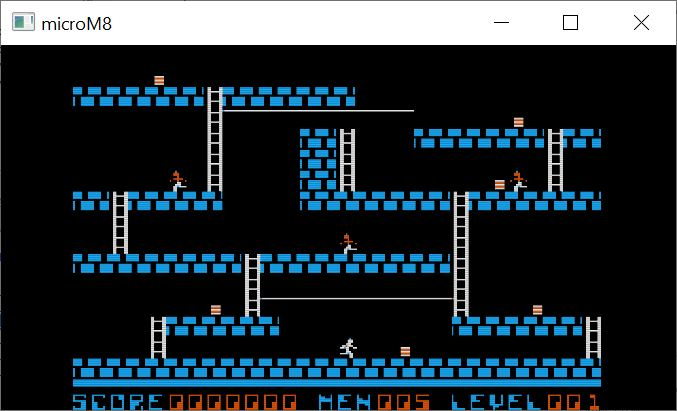
\includegraphics[width=\columnwidth]{screen}
\end{center}

There's a routine to add a 4-digit BCD
number to the score and then update it on the screen.

\nwenddocs{}\nwbegincode{82}\sublabel{NW1Xx3lK-J3zE9-1}\nwmargintag{{\nwtagstyle{}\subpageref{NW1Xx3lK-J3zE9-1}}}\moddef{add and update score~{\nwtagstyle{}\subpageref{NW1Xx3lK-J3zE9-1}}}\endmoddef\nwstartdeflinemarkup\nwusesondefline{\\{NW1Xx3lK-8jv1b-C}}\nwenddeflinemarkup
    ORG     $7A92
\nwlinkedidentc{ADD_AND_UPDATE_SCORE}{NW1Xx3lK-J3zE9-1}:
    SUBROUTINE
    ; Enter routine with A set to BCD tens/units and
    ; Y set to BCD thousands/hundreds.

    CLC
    SED                         ; Turn on BCD addition mode.
    ADC     \nwlinkedidentc{SCORE}{NW1Xx3lK-10jlgu-C}
    STA     \nwlinkedidentc{SCORE}{NW1Xx3lK-10jlgu-C}
    TYA
    ADC     \nwlinkedidentc{SCORE}{NW1Xx3lK-10jlgu-C}+1
    STA     \nwlinkedidentc{SCORE}{NW1Xx3lK-10jlgu-C}+1
    LDA     #$00
    ADC     \nwlinkedidentc{SCORE}{NW1Xx3lK-10jlgu-C}+2
    STA     \nwlinkedidentc{SCORE}{NW1Xx3lK-10jlgu-C}+2
    LDA     #$00
    ADC     \nwlinkedidentc{SCORE}{NW1Xx3lK-10jlgu-C}+3
    STA     \nwlinkedidentc{SCORE}{NW1Xx3lK-10jlgu-C}+3             ; \nwlinkedidentc{SCORE}{NW1Xx3lK-10jlgu-C} += param
    CLD                         ; Turn off BCD addition mode.

    LDA     #5
    STA     \nwlinkedidentc{GAME_COLNUM}{NW1Xx3lK-10jlgu-7}
    LDA     #16
    STA     \nwlinkedidentc{GAME_ROWNUM}{NW1Xx3lK-10jlgu-7}

    LDA     \nwlinkedidentc{SCORE}{NW1Xx3lK-10jlgu-C}+3
    JSR     \nwlinkedidentc{BCD_TO_DECIMAL2}{NW1Xx3lK-27Rk8U-1}
    LDA     \nwlinkedidentc{UNITS}{NW1Xx3lK-10jlgu-B}               ; Note we skipped \nwlinkedidentc{TENS}{NW1Xx3lK-10jlgu-B}.
    JSR     \nwlinkedidentc{PUT_DIGIT}{NW1Xx3lK-3fFmzP-1}

    LDA     \nwlinkedidentc{SCORE}{NW1Xx3lK-10jlgu-C}+2
    JSR     \nwlinkedidentc{BCD_TO_DECIMAL2}{NW1Xx3lK-27Rk8U-1}
    LDA     \nwlinkedidentc{TENS}{NW1Xx3lK-10jlgu-B}
    JSR     \nwlinkedidentc{PUT_DIGIT}{NW1Xx3lK-3fFmzP-1}
    LDA     \nwlinkedidentc{UNITS}{NW1Xx3lK-10jlgu-B}
    JSR     \nwlinkedidentc{PUT_DIGIT}{NW1Xx3lK-3fFmzP-1}

    LDA     \nwlinkedidentc{SCORE}{NW1Xx3lK-10jlgu-C}+1
    JSR     \nwlinkedidentc{BCD_TO_DECIMAL2}{NW1Xx3lK-27Rk8U-1}
    LDA     \nwlinkedidentc{TENS}{NW1Xx3lK-10jlgu-B}
    JSR     \nwlinkedidentc{PUT_DIGIT}{NW1Xx3lK-3fFmzP-1}
    LDA     \nwlinkedidentc{UNITS}{NW1Xx3lK-10jlgu-B}
    JSR     \nwlinkedidentc{PUT_DIGIT}{NW1Xx3lK-3fFmzP-1}

    LDA     \nwlinkedidentc{SCORE}{NW1Xx3lK-10jlgu-C}
    JSR     \nwlinkedidentc{BCD_TO_DECIMAL2}{NW1Xx3lK-27Rk8U-1}
    LDA     \nwlinkedidentc{TENS}{NW1Xx3lK-10jlgu-B}
    JSR     \nwlinkedidentc{PUT_DIGIT}{NW1Xx3lK-3fFmzP-1}
    LDA     \nwlinkedidentc{UNITS}{NW1Xx3lK-10jlgu-B}
    JMP     \nwlinkedidentc{PUT_DIGIT}{NW1Xx3lK-3fFmzP-1}           ; tail call

\nwindexdefn{\nwixident{ADD{\_}AND{\_}UPDATE{\_}SCORE}}{ADD:unAND:unUPDATE:unSCORE}{NW1Xx3lK-J3zE9-1}\eatline
\nwused{\\{NW1Xx3lK-8jv1b-C}}\nwidentdefs{\\{{\nwixident{ADD{\_}AND{\_}UPDATE{\_}SCORE}}{ADD:unAND:unUPDATE:unSCORE}}}\nwidentuses{\\{{\nwixident{BCD{\_}TO{\_}DECIMAL2}}{BCD:unTO:unDECIMAL2}}\\{{\nwixident{GAME{\_}COLNUM}}{GAME:unCOLNUM}}\\{{\nwixident{GAME{\_}ROWNUM}}{GAME:unROWNUM}}\\{{\nwixident{PUT{\_}DIGIT}}{PUT:unDIGIT}}\\{{\nwixident{SCORE}}{SCORE}}\\{{\nwixident{TENS}}{TENS}}\\{{\nwixident{UNITS}}{UNITS}}}\nwindexuse{\nwixident{BCD{\_}TO{\_}DECIMAL2}}{BCD:unTO:unDECIMAL2}{NW1Xx3lK-J3zE9-1}\nwindexuse{\nwixident{GAME{\_}COLNUM}}{GAME:unCOLNUM}{NW1Xx3lK-J3zE9-1}\nwindexuse{\nwixident{GAME{\_}ROWNUM}}{GAME:unROWNUM}{NW1Xx3lK-J3zE9-1}\nwindexuse{\nwixident{PUT{\_}DIGIT}}{PUT:unDIGIT}{NW1Xx3lK-J3zE9-1}\nwindexuse{\nwixident{SCORE}}{SCORE}{NW1Xx3lK-J3zE9-1}\nwindexuse{\nwixident{TENS}}{TENS}{NW1Xx3lK-J3zE9-1}\nwindexuse{\nwixident{UNITS}}{UNITS}{NW1Xx3lK-J3zE9-1}\nwendcode{}\nwbegindocs{83}\nwdocspar
The other elements in the status line are the number of men
(i.e. lives) and the current level.

\nwenddocs{}\nwbegincode{84}\sublabel{NW1Xx3lK-10jlgu-D}\nwmargintag{{\nwtagstyle{}\subpageref{NW1Xx3lK-10jlgu-D}}}\moddef{defines~{\nwtagstyle{}\subpageref{NW1Xx3lK-10jlgu-1}}}\plusendmoddef\nwstartdeflinemarkup\nwusesondefline{\\{NW1Xx3lK-1p0Y9w-1}}\nwprevnextdefs{NW1Xx3lK-10jlgu-C}{NW1Xx3lK-10jlgu-E}\nwenddeflinemarkup
\nwlinkedidentc{LEVELNUM}{NW1Xx3lK-10jlgu-D}    EQU     $A6
\nwlinkedidentc{LIVES}{NW1Xx3lK-10jlgu-D}       EQU     $98
\nwindexdefn{\nwixident{LEVELNUM}}{LEVELNUM}{NW1Xx3lK-10jlgu-D}\nwindexdefn{\nwixident{LIVES}}{LIVES}{NW1Xx3lK-10jlgu-D}\eatline
\nwused{\\{NW1Xx3lK-1p0Y9w-1}}\nwidentdefs{\\{{\nwixident{LEVELNUM}}{LEVELNUM}}\\{{\nwixident{LIVES}}{LIVES}}}\nwendcode{}\nwbegindocs{85}\nwdocspar
Here are the routines to put the lives and level number on
the status line. Lives starts at column 16, and level number
starts at column 25.

\nwenddocs{}\nwbegincode{86}\sublabel{NW1Xx3lK-458dZ9-1}\nwmargintag{{\nwtagstyle{}\subpageref{NW1Xx3lK-458dZ9-1}}}\moddef{put status~{\nwtagstyle{}\subpageref{NW1Xx3lK-458dZ9-1}}}\endmoddef\nwstartdeflinemarkup\nwusesondefline{\\{NW1Xx3lK-8jv1b-C}}\nwenddeflinemarkup
    ORG     $7A70
\nwlinkedidentc{PUT_STATUS_LIVES}{NW1Xx3lK-458dZ9-1}:
    SUBROUTINE

    LDA     \nwlinkedidentc{LIVES}{NW1Xx3lK-10jlgu-D}
    LDX     #16
    ; fallthrough

PUT_STATUS_BYTE:
    SUBROUTINE
    ; Puts the number in A as a three-digit decimal on the screen
    ; at row 16, column X.

    STX     \nwlinkedidentc{GAME_COLNUM}{NW1Xx3lK-10jlgu-7}
    JSR     \nwlinkedidentc{TO_DECIMAL3}{NW1Xx3lK-1LYsFk-1}
    LDA     #16
    STA     \nwlinkedidentc{GAME_ROWNUM}{NW1Xx3lK-10jlgu-7}
    LDA     \nwlinkedidentc{HUNDREDS}{NW1Xx3lK-10jlgu-B}
    JSR     \nwlinkedidentc{PUT_DIGIT}{NW1Xx3lK-3fFmzP-1}
    LDA     \nwlinkedidentc{TENS}{NW1Xx3lK-10jlgu-B}
    JSR     \nwlinkedidentc{PUT_DIGIT}{NW1Xx3lK-3fFmzP-1}
    LDA     \nwlinkedidentc{UNITS}{NW1Xx3lK-10jlgu-B}
    JMP     \nwlinkedidentc{PUT_DIGIT}{NW1Xx3lK-3fFmzP-1}           ; tail call

\nwlinkedidentc{PUT_STATUS_LEVEL}{NW1Xx3lK-458dZ9-1}:
    SUBROUTINE

    LDA     \nwlinkedidentc{LEVELNUM}{NW1Xx3lK-10jlgu-D}
    LDX     #25
    BNE     PUT_STATUS_BYTE     ; Unconditional jump

    ORG     $79AD
\nwlinkedidentc{PUT_STATUS}{NW1Xx3lK-458dZ9-1}:
    SUBROUTINE

    JSR     \nwlinkedidentc{CLEAR_HGR1}{NW1Xx3lK-8jv1b-1}
    JSR     \nwlinkedidentc{CLEAR_HGR2}{NW1Xx3lK-8jv1b-1}

PUT_STATUS_DRAW:
    LDY     #$27
    LDA     \nwlinkedidentc{DRAW_PAGE}{NW1Xx3lK-10jlgu-9}
    CMP     #$40
    BEQ     .draw_line_on_page_2

.draw_line_on_page_1:
    LDA     #$AA
    STA     $2350,Y
    STA     $2750,Y
    STA     $2B50,Y
    STA     $2F50,Y
    DEY
    LDA     #$D5
    STA     $2350,Y
    STA     $2750,Y
    STA     $2B50,Y
    STA     $2F50,Y
    DEY
    BPL     .draw_line_on_page_1
    BMI     .end        ; Unconditional

.draw_line_on_page_2:
    LDA     #$AA
    STA     $4350,Y
    STA     $4750,Y
    STA     $4B50,Y
    STA     $4F50,Y
    DEY
    LDA     #$D5
    STA     $4350,Y
    STA     $4750,Y
    STA     $4B50,Y
    STA     $4F50,Y
    DEY
    BPL     .draw_line_on_page_2

.end:
    LDA     #$10
    STA     \nwlinkedidentc{GAME_ROWNUM}{NW1Xx3lK-10jlgu-7}
    LDA     #$00
    STA     \nwlinkedidentc{GAME_COLNUM}{NW1Xx3lK-10jlgu-7}

    ; "\nwlinkedidentc{SCORE}{NW1Xx3lK-10jlgu-C}        MEN    LEVEL   "
    JSR     \nwlinkedidentc{PUT_STRING}{NW1Xx3lK-47YPHz-1}
    HEX     D3 C3 CF D2 C5 A0 A0 A0 A0 A0 A0 A0 A0 CD C5 CE
    HEX     A0 A0 A0 A0 CC C5 D6 C5 CC A0 A0 A0 00

    JSR     \nwlinkedidentc{PUT_STATUS_LIVES}{NW1Xx3lK-458dZ9-1}
    JSR     \nwlinkedidentc{PUT_STATUS_LEVEL}{NW1Xx3lK-458dZ9-1}
    LDA     #$00
    TAY
    JMP     \nwlinkedidentc{ADD_AND_UPDATE_SCORE}{NW1Xx3lK-J3zE9-1}        ; tailcall

\nwindexdefn{\nwixident{PUT{\_}STATUS{\_}LIVES}}{PUT:unSTATUS:unLIVES}{NW1Xx3lK-458dZ9-1}\nwindexdefn{\nwixident{PUT{\_}STATUS{\_}LEVEL}}{PUT:unSTATUS:unLEVEL}{NW1Xx3lK-458dZ9-1}\nwindexdefn{\nwixident{PUT{\_}STATUS}}{PUT:unSTATUS}{NW1Xx3lK-458dZ9-1}\eatline
\nwused{\\{NW1Xx3lK-8jv1b-C}}\nwidentdefs{\\{{\nwixident{PUT{\_}STATUS}}{PUT:unSTATUS}}\\{{\nwixident{PUT{\_}STATUS{\_}LEVEL}}{PUT:unSTATUS:unLEVEL}}\\{{\nwixident{PUT{\_}STATUS{\_}LIVES}}{PUT:unSTATUS:unLIVES}}}\nwidentuses{\\{{\nwixident{ADD{\_}AND{\_}UPDATE{\_}SCORE}}{ADD:unAND:unUPDATE:unSCORE}}\\{{\nwixident{CLEAR{\_}HGR1}}{CLEAR:unHGR1}}\\{{\nwixident{CLEAR{\_}HGR2}}{CLEAR:unHGR2}}\\{{\nwixident{DRAW{\_}PAGE}}{DRAW:unPAGE}}\\{{\nwixident{GAME{\_}COLNUM}}{GAME:unCOLNUM}}\\{{\nwixident{GAME{\_}ROWNUM}}{GAME:unROWNUM}}\\{{\nwixident{HUNDREDS}}{HUNDREDS}}\\{{\nwixident{LEVELNUM}}{LEVELNUM}}\\{{\nwixident{LIVES}}{LIVES}}\\{{\nwixident{PUT{\_}DIGIT}}{PUT:unDIGIT}}\\{{\nwixident{PUT{\_}STRING}}{PUT:unSTRING}}\\{{\nwixident{SCORE}}{SCORE}}\\{{\nwixident{TENS}}{TENS}}\\{{\nwixident{TO{\_}DECIMAL3}}{TO:unDECIMAL3}}\\{{\nwixident{UNITS}}{UNITS}}}\nwindexuse{\nwixident{ADD{\_}AND{\_}UPDATE{\_}SCORE}}{ADD:unAND:unUPDATE:unSCORE}{NW1Xx3lK-458dZ9-1}\nwindexuse{\nwixident{CLEAR{\_}HGR1}}{CLEAR:unHGR1}{NW1Xx3lK-458dZ9-1}\nwindexuse{\nwixident{CLEAR{\_}HGR2}}{CLEAR:unHGR2}{NW1Xx3lK-458dZ9-1}\nwindexuse{\nwixident{DRAW{\_}PAGE}}{DRAW:unPAGE}{NW1Xx3lK-458dZ9-1}\nwindexuse{\nwixident{GAME{\_}COLNUM}}{GAME:unCOLNUM}{NW1Xx3lK-458dZ9-1}\nwindexuse{\nwixident{GAME{\_}ROWNUM}}{GAME:unROWNUM}{NW1Xx3lK-458dZ9-1}\nwindexuse{\nwixident{HUNDREDS}}{HUNDREDS}{NW1Xx3lK-458dZ9-1}\nwindexuse{\nwixident{LEVELNUM}}{LEVELNUM}{NW1Xx3lK-458dZ9-1}\nwindexuse{\nwixident{LIVES}}{LIVES}{NW1Xx3lK-458dZ9-1}\nwindexuse{\nwixident{PUT{\_}DIGIT}}{PUT:unDIGIT}{NW1Xx3lK-458dZ9-1}\nwindexuse{\nwixident{PUT{\_}STRING}}{PUT:unSTRING}{NW1Xx3lK-458dZ9-1}\nwindexuse{\nwixident{SCORE}}{SCORE}{NW1Xx3lK-458dZ9-1}\nwindexuse{\nwixident{TENS}}{TENS}{NW1Xx3lK-458dZ9-1}\nwindexuse{\nwixident{TO{\_}DECIMAL3}}{TO:unDECIMAL3}{NW1Xx3lK-458dZ9-1}\nwindexuse{\nwixident{UNITS}}{UNITS}{NW1Xx3lK-458dZ9-1}\nwendcode{}\nwbegindocs{87}\nwdocspar
\chapter{Sound}

\section{Simple beep}

This simple beep routine clicks the speaker every 656 cycles. At approximately 980 nsec per cycle, this would
be a period of about 0.64 milliseconds, or a tone of 1.56 kHz. This is a short beep, playing for a little over
0.1 seconds.

\nwenddocs{}\nwbegincode{88}\sublabel{NW1Xx3lK-dU9NC-1}\nwmargintag{{\nwtagstyle{}\subpageref{NW1Xx3lK-dU9NC-1}}}\moddef{beep~{\nwtagstyle{}\subpageref{NW1Xx3lK-dU9NC-1}}}\endmoddef\nwstartdeflinemarkup\nwusesondefline{\\{NW1Xx3lK-8jv1b-C}}\nwenddeflinemarkup
    ORG     $86CE
\nwlinkedidentc{BEEP}{NW1Xx3lK-dU9NC-1}:
    SUBROUTINE

    LDY     #$C0

.loop:
    ; From here to click is 651 cycles. Additional 5 cycles afterwards.
    LDX     #$80            ; 2 cycles

    ; delay 640 cycles
.loop2:
    DEX                     ; 2 cycles
    BNE     .loop2          ; 3 cycles

    LDA     \nwlinkedidentc{ENABLE_SOUND}{NW1Xx3lK-10jlgu-F}    ; 3 cycles
    BEQ     .next           ; 3 cycles
    LDA     \nwlinkedidentc{SPKR}{NW1Xx3lK-10jlgu-F}            ; 3 cycles

.next:
    DEY                     ; 2 cycles
    BNE     .loop           ; 3 cycles
    RTS
\nwindexdefn{\nwixident{BEEP}}{BEEP}{NW1Xx3lK-dU9NC-1}\eatline
\nwused{\\{NW1Xx3lK-8jv1b-C}}\nwidentdefs{\\{{\nwixident{BEEP}}{BEEP}}}\nwidentuses{\\{{\nwixident{ENABLE{\_}SOUND}}{ENABLE:unSOUND}}\\{{\nwixident{SPKR}}{SPKR}}}\nwindexuse{\nwixident{ENABLE{\_}SOUND}}{ENABLE:unSOUND}{NW1Xx3lK-dU9NC-1}\nwindexuse{\nwixident{SPKR}}{SPKR}{NW1Xx3lK-dU9NC-1}\nwendcode{}\nwbegindocs{89}\nwdocspar

\section{Sound "strings"}

A sound "string" describes a sound to play in terms of pitch and duration, ending in a {\Tt{}00\nwendquote}.
Just like in the {\Tt{}\nwlinkedidentq{PUT{\_}STRING}{NW1Xx3lK-47YPHz-1}\nwendquote} routine, rather than take
an address pointing to a sound string, instead it uses the return address as the source for data.
It then has to fix up the actual return address at the end to be just after the zero-terminating
byte of the string.

Because {\Tt{}\nwlinkedidentq{NOTE{\_}INDEX}{NW1Xx3lK-10jlgu-E}\nwendquote} is not zeroed out, this actually appends to the sound data buffer.

The format of a sound string is duration, followed by pitch, although the pitch is lower for higher numbers.

One example of a sound string is {\Tt{}07\ 45\ 06\ 55\ 05\ 44\ 04\ 54\ 03\ 43\ 02\ 53\nwendquote}, found in {\Tt{}\nwlinkedidentq{CHECK{\_}FOR{\_}GOLD{\_}PICKED{\_}UP{\_}BY{\_}PLAYER}{NW1Xx3lK-2zzVjv-1}\nwendquote}.


\nwenddocs{}\nwbegincode{90}\sublabel{NW1Xx3lK-10jlgu-E}\nwmargintag{{\nwtagstyle{}\subpageref{NW1Xx3lK-10jlgu-E}}}\moddef{defines~{\nwtagstyle{}\subpageref{NW1Xx3lK-10jlgu-1}}}\plusendmoddef\nwstartdeflinemarkup\nwusesondefline{\\{NW1Xx3lK-1p0Y9w-1}}\nwprevnextdefs{NW1Xx3lK-10jlgu-D}{NW1Xx3lK-10jlgu-F}\nwenddeflinemarkup
\nwlinkedidentc{NOTE_INDEX}{NW1Xx3lK-10jlgu-E}      EQU     $54
\nwlinkedidentc{SOUND_DURATION}{NW1Xx3lK-10jlgu-E}  EQU     $0E00       ; 128 bytes
\nwlinkedidentc{SOUND_PITCH}{NW1Xx3lK-10jlgu-E}     EQU     $0E80       ; 128 bytes
\nwindexdefn{\nwixident{NOTE{\_}INDEX}}{NOTE:unINDEX}{NW1Xx3lK-10jlgu-E}\nwindexdefn{\nwixident{SOUND{\_}DURATION}}{SOUND:unDURATION}{NW1Xx3lK-10jlgu-E}\nwindexdefn{\nwixident{SOUND{\_}PITCH}}{SOUND:unPITCH}{NW1Xx3lK-10jlgu-E}\eatline
\nwused{\\{NW1Xx3lK-1p0Y9w-1}}\nwidentdefs{\\{{\nwixident{NOTE{\_}INDEX}}{NOTE:unINDEX}}\\{{\nwixident{SOUND{\_}DURATION}}{SOUND:unDURATION}}\\{{\nwixident{SOUND{\_}PITCH}}{SOUND:unPITCH}}}\nwendcode{}\nwbegindocs{91}\nwdocspar
\nwenddocs{}\nwbegincode{92}\sublabel{NW1Xx3lK-90gdY-1}\nwmargintag{{\nwtagstyle{}\subpageref{NW1Xx3lK-90gdY-1}}}\moddef{load sound data~{\nwtagstyle{}\subpageref{NW1Xx3lK-90gdY-1}}}\endmoddef\nwstartdeflinemarkup\nwusesondefline{\\{NW1Xx3lK-8jv1b-C}}\nwenddeflinemarkup
    ORG     $87E1
\nwlinkedidentc{LOAD_SOUND_DATA}{NW1Xx3lK-90gdY-1}:
    SUBROUTINE

    PLA
    STA     \nwlinkedidentc{SAVED_RET_ADDR}{NW1Xx3lK-10jlgu-A}
    PLA
    STA     \nwlinkedidentc{SAVED_RET_ADDR}{NW1Xx3lK-10jlgu-A}+1
    BNE     .next

.loop:
    LDY     #$00
    LDA     (\nwlinkedidentc{SAVED_RET_ADDR}{NW1Xx3lK-10jlgu-A}),Y
    BEQ     .end
    INC     \nwlinkedidentc{NOTE_INDEX}{NW1Xx3lK-10jlgu-E}
    LDX     \nwlinkedidentc{NOTE_INDEX}{NW1Xx3lK-10jlgu-E}
    STA     \nwlinkedidentc{SOUND_DURATION}{NW1Xx3lK-10jlgu-E},X
    INY
    LDA     (\nwlinkedidentc{SAVED_RET_ADDR}{NW1Xx3lK-10jlgu-A}),Y
    STA     \nwlinkedidentc{SOUND_PITCH}{NW1Xx3lK-10jlgu-E},X

    INC     \nwlinkedidentc{SAVED_RET_ADDR}{NW1Xx3lK-10jlgu-A}
    BNE     .next
    INC     \nwlinkedidentc{SAVED_RET_ADDR}{NW1Xx3lK-10jlgu-A}+1

.next:
    INC     \nwlinkedidentc{SAVED_RET_ADDR}{NW1Xx3lK-10jlgu-A}
    BNE     .loop
    INC     \nwlinkedidentc{SAVED_RET_ADDR}{NW1Xx3lK-10jlgu-A}+1
    BNE     .loop

.end:
    LDA     \nwlinkedidentc{SAVED_RET_ADDR}{NW1Xx3lK-10jlgu-A}+1
    PHA
    LDA     \nwlinkedidentc{SAVED_RET_ADDR}{NW1Xx3lK-10jlgu-A}
    PHA
    RTS
\nwindexdefn{\nwixident{LOAD{\_}SOUND{\_}DATA}}{LOAD:unSOUND:unDATA}{NW1Xx3lK-90gdY-1}\eatline
\nwused{\\{NW1Xx3lK-8jv1b-C}}\nwidentdefs{\\{{\nwixident{LOAD{\_}SOUND{\_}DATA}}{LOAD:unSOUND:unDATA}}}\nwidentuses{\\{{\nwixident{NOTE{\_}INDEX}}{NOTE:unINDEX}}\\{{\nwixident{SAVED{\_}RET{\_}ADDR}}{SAVED:unRET:unADDR}}\\{{\nwixident{SOUND{\_}DURATION}}{SOUND:unDURATION}}\\{{\nwixident{SOUND{\_}PITCH}}{SOUND:unPITCH}}}\nwindexuse{\nwixident{NOTE{\_}INDEX}}{NOTE:unINDEX}{NW1Xx3lK-90gdY-1}\nwindexuse{\nwixident{SAVED{\_}RET{\_}ADDR}}{SAVED:unRET:unADDR}{NW1Xx3lK-90gdY-1}\nwindexuse{\nwixident{SOUND{\_}DURATION}}{SOUND:unDURATION}{NW1Xx3lK-90gdY-1}\nwindexuse{\nwixident{SOUND{\_}PITCH}}{SOUND:unPITCH}{NW1Xx3lK-90gdY-1}\nwendcode{}\nwbegindocs{93}\nwdocspar
There's also a simple routine to append a single note to the sound buffer. The routine gets
called with the pitch in {\Tt{}A\nwendquote} and the duration in {\Tt{}X\nwendquote}.

\nwenddocs{}\nwbegincode{94}\sublabel{NW1Xx3lK-4JsOpf-1}\nwmargintag{{\nwtagstyle{}\subpageref{NW1Xx3lK-4JsOpf-1}}}\moddef{append note~{\nwtagstyle{}\subpageref{NW1Xx3lK-4JsOpf-1}}}\endmoddef\nwstartdeflinemarkup\nwusesondefline{\\{NW1Xx3lK-8jv1b-C}}\nwenddeflinemarkup
    ORG     $87D5
\nwlinkedidentc{APPEND_NOTE}{NW1Xx3lK-4JsOpf-1}:
    SUBROUTINE

    INC     \nwlinkedidentc{NOTE_INDEX}{NW1Xx3lK-10jlgu-E}
    LDY     \nwlinkedidentc{NOTE_INDEX}{NW1Xx3lK-10jlgu-E}
    STA     \nwlinkedidentc{SOUND_PITCH}{NW1Xx3lK-10jlgu-E},Y
    TXA
    STA     \nwlinkedidentc{SOUND_DURATION}{NW1Xx3lK-10jlgu-E},Y
    RTS
\nwindexdefn{\nwixident{APPEND{\_}NOTE}}{APPEND:unNOTE}{NW1Xx3lK-4JsOpf-1}\eatline
\nwused{\\{NW1Xx3lK-8jv1b-C}}\nwidentdefs{\\{{\nwixident{APPEND{\_}NOTE}}{APPEND:unNOTE}}}\nwidentuses{\\{{\nwixident{NOTE{\_}INDEX}}{NOTE:unINDEX}}\\{{\nwixident{SOUND{\_}DURATION}}{SOUND:unDURATION}}\\{{\nwixident{SOUND{\_}PITCH}}{SOUND:unPITCH}}}\nwindexuse{\nwixident{NOTE{\_}INDEX}}{NOTE:unINDEX}{NW1Xx3lK-4JsOpf-1}\nwindexuse{\nwixident{SOUND{\_}DURATION}}{SOUND:unDURATION}{NW1Xx3lK-4JsOpf-1}\nwindexuse{\nwixident{SOUND{\_}PITCH}}{SOUND:unPITCH}{NW1Xx3lK-4JsOpf-1}\nwendcode{}\nwbegindocs{95}\nwdocspar
\section{Playing notes}

The {\Tt{}\nwlinkedidentq{PLAY{\_}NOTE}{NW1Xx3lK-1Ew0EG-1}\nwendquote} routines plays a note through the built-in speaker. The time the note is played is
based on {\Tt{}X\nwendquote} and {\Tt{}Y\nwendquote} forming a 16-bit counter ({\Tt{}X\nwendquote} being the most significant byte), but {\Tt{}A\nwendquote} controls the pitch,
which is how often the speaker is clicked. The higher {\Tt{}A\nwendquote}, the lower the pitch.

The {\Tt{}\nwlinkedidentq{ENABLE{\_}SOUND}{NW1Xx3lK-10jlgu-F}\nwendquote} location can also disable playing the note, but the routine still takes as long as it would have.

\nwenddocs{}\nwbegincode{96}\sublabel{NW1Xx3lK-10jlgu-F}\nwmargintag{{\nwtagstyle{}\subpageref{NW1Xx3lK-10jlgu-F}}}\moddef{defines~{\nwtagstyle{}\subpageref{NW1Xx3lK-10jlgu-1}}}\plusendmoddef\nwstartdeflinemarkup\nwusesondefline{\\{NW1Xx3lK-1p0Y9w-1}}\nwprevnextdefs{NW1Xx3lK-10jlgu-E}{NW1Xx3lK-10jlgu-G}\nwenddeflinemarkup
\nwlinkedidentc{ENABLE_SOUND}{NW1Xx3lK-10jlgu-F}    EQU     $99     ; If 0, do not click speaker.
\nwlinkedidentc{SPKR}{NW1Xx3lK-10jlgu-F}            EQU     $C030   ; Access clicks the speaker.
\nwindexdefn{\nwixident{ENABLE{\_}SOUND}}{ENABLE:unSOUND}{NW1Xx3lK-10jlgu-F}\nwindexdefn{\nwixident{SPKR}}{SPKR}{NW1Xx3lK-10jlgu-F}\eatline
\nwused{\\{NW1Xx3lK-1p0Y9w-1}}\nwidentdefs{\\{{\nwixident{ENABLE{\_}SOUND}}{ENABLE:unSOUND}}\\{{\nwixident{SPKR}}{SPKR}}}\nwendcode{}\nwbegindocs{97}\nwdocspar
\nwenddocs{}\nwbegincode{98}\sublabel{NW1Xx3lK-1Ew0EG-1}\nwmargintag{{\nwtagstyle{}\subpageref{NW1Xx3lK-1Ew0EG-1}}}\moddef{play note~{\nwtagstyle{}\subpageref{NW1Xx3lK-1Ew0EG-1}}}\endmoddef\nwstartdeflinemarkup\nwusesondefline{\\{NW1Xx3lK-8jv1b-C}}\nwenddeflinemarkup
    ORG     $87BA
\nwlinkedidentc{PLAY_NOTE}{NW1Xx3lK-1Ew0EG-1}:
    SUBROUTINE

    STA     \nwlinkedidentc{TMP_PTR}{NW1Xx3lK-10jlgu-1}
    STX     \nwlinkedidentc{TMP_PTR}{NW1Xx3lK-10jlgu-1}+1

.loop:
    LDA     \nwlinkedidentc{ENABLE_SOUND}{NW1Xx3lK-10jlgu-F}
    BEQ     .decrement_counter
    LDA     \nwlinkedidentc{SPKR}{NW1Xx3lK-10jlgu-F}

.decrement_counter:
    DEY
    BNE     .counter_decremented
    DEC     \nwlinkedidentc{TMP_PTR}{NW1Xx3lK-10jlgu-1}+1
    BEQ     .end

.counter_decremented:
    DEX
    BNE     .decrement_counter
    LDX     \nwlinkedidentc{TMP_PTR}{NW1Xx3lK-10jlgu-1}
    JMP     .loop

.end:
    RTS
\nwindexdefn{\nwixident{PLAY{\_}NOTE}}{PLAY:unNOTE}{NW1Xx3lK-1Ew0EG-1}\eatline
\nwused{\\{NW1Xx3lK-8jv1b-C}}\nwidentdefs{\\{{\nwixident{PLAY{\_}NOTE}}{PLAY:unNOTE}}}\nwidentuses{\\{{\nwixident{ENABLE{\_}SOUND}}{ENABLE:unSOUND}}\\{{\nwixident{SPKR}}{SPKR}}\\{{\nwixident{TMP{\_}PTR}}{TMP:unPTR}}}\nwindexuse{\nwixident{ENABLE{\_}SOUND}}{ENABLE:unSOUND}{NW1Xx3lK-1Ew0EG-1}\nwindexuse{\nwixident{SPKR}}{SPKR}{NW1Xx3lK-1Ew0EG-1}\nwindexuse{\nwixident{TMP{\_}PTR}}{TMP:unPTR}{NW1Xx3lK-1Ew0EG-1}\nwendcode{}\nwbegindocs{99}\nwdocspar
\section{Playing a sound}

The {\Tt{}\nwlinkedidentq{SOUND{\_}DELAY}{NW1Xx3lK-3j1fAh-1}\nwendquote} routine delays an amount of time based on the X register. The total number of cycles is about 905 per each X.
Since the Apple //e clock cycle was 980 nsec (on an NTSC system), this routine would delay approximately 887 microseconds times X.
PAL systems were very slightly slower (by $0.47\%$), which corresponds to 883 microseconds times X.

\nwenddocs{}\nwbegincode{100}\sublabel{NW1Xx3lK-1W8AJS-A}\nwmargintag{{\nwtagstyle{}\subpageref{NW1Xx3lK-1W8AJS-A}}}\moddef{tables~{\nwtagstyle{}\subpageref{NW1Xx3lK-1W8AJS-1}}}\plusendmoddef\nwstartdeflinemarkup\nwusesondefline{\\{NW1Xx3lK-1p0Y9w-1}}\nwprevnextdefs{NW1Xx3lK-1W8AJS-9}{NW1Xx3lK-1W8AJS-B}\nwenddeflinemarkup
    ORG     $86BE
\nwlinkedidentc{SOUND_DELAY_AMOUNTS}{NW1Xx3lK-1W8AJS-A}:
    HEX     02 04 06 08 0A 0C 0E 10 12 14 16 18 1A 1C 1E 20
\nwindexdefn{\nwixident{SOUND{\_}DELAY{\_}AMOUNTS}}{SOUND:unDELAY:unAMOUNTS}{NW1Xx3lK-1W8AJS-A}\eatline
\nwused{\\{NW1Xx3lK-1p0Y9w-1}}\nwidentdefs{\\{{\nwixident{SOUND{\_}DELAY{\_}AMOUNTS}}{SOUND:unDELAY:unAMOUNTS}}}\nwendcode{}\nwbegindocs{101}\nwdocspar
\nwenddocs{}\nwbegincode{102}\sublabel{NW1Xx3lK-3j1fAh-1}\nwmargintag{{\nwtagstyle{}\subpageref{NW1Xx3lK-3j1fAh-1}}}\moddef{sound delay~{\nwtagstyle{}\subpageref{NW1Xx3lK-3j1fAh-1}}}\endmoddef\nwstartdeflinemarkup\nwusesondefline{\\{NW1Xx3lK-8jv1b-C}}\nwenddeflinemarkup
    ORG     $86B1
\nwlinkedidentc{SOUND_DELAY}{NW1Xx3lK-3j1fAh-1}:
    SUBROUTINE

    LDA     \nwlinkedidentc{SOUND_DELAY_AMOUNTS}{NW1Xx3lK-1W8AJS-A},X
    TAX

\nwlinkedidentc{SOUND_DELAY1}{NW1Xx3lK-3j1fAh-1}:
    LDY     #$B4         ; 180
.loop:
    DEY                  ; 2 cycles
    BNE     .loop        ; 3 cycles
    DEX                  ; 2 cycles
    BNE     \nwlinkedidentc{SOUND_DELAY1}{NW1Xx3lK-3j1fAh-1} ; 3 cycles
    RTS
\nwindexdefn{\nwixident{SOUND{\_}DELAY}}{SOUND:unDELAY}{NW1Xx3lK-3j1fAh-1}\nwindexdefn{\nwixident{SOUND{\_}DELAY1}}{SOUND:unDELAY1}{NW1Xx3lK-3j1fAh-1}\eatline
\nwused{\\{NW1Xx3lK-8jv1b-C}}\nwidentdefs{\\{{\nwixident{SOUND{\_}DELAY}}{SOUND:unDELAY}}\\{{\nwixident{SOUND{\_}DELAY1}}{SOUND:unDELAY1}}}\nwidentuses{\\{{\nwixident{SOUND{\_}DELAY{\_}AMOUNTS}}{SOUND:unDELAY:unAMOUNTS}}}\nwindexuse{\nwixident{SOUND{\_}DELAY{\_}AMOUNTS}}{SOUND:unDELAY:unAMOUNTS}{NW1Xx3lK-3j1fAh-1}\nwendcode{}\nwbegindocs{103}\nwdocspar

Finally, the {\Tt{}\nwlinkedidentq{PLAY{\_}SOUND}{NW1Xx3lK-4DEk44-1}\nwendquote} routine plays one section of the sound string stored in the {\Tt{}\nwlinkedidentq{SOUND{\_}PITCH}{NW1Xx3lK-10jlgu-E}\nwendquote}
and {\Tt{}\nwlinkedidentq{SOUND{\_}DURATION}{NW1Xx3lK-10jlgu-E}\nwendquote} buffers. We have to break up the playing of the sound so that gameplay doesn't
pause while playing the sound, although game play does pause while playing the note.

Alternatively, if there is no sound string, we can play the note stored in location {\Tt{}{\nwbackslash}{\$}A4\nwendquote} as long as
location {\Tt{}{\nwbackslash}{\$}9B\nwendquote} is zero. The duration is {\Tt{}2\ +\ \nwlinkedidentq{FRAME{\_}PERIOD}{NW1Xx3lK-10jlgu-G}\nwendquote}.

The routine is designed to delay approximately the same amount regardless of sound duration. The
delay is controlled by {\Tt{}\nwlinkedidentq{FRAME{\_}PERIOD}{NW1Xx3lK-10jlgu-G}\nwendquote}. This value is hardcoded to {\Tt{}6\nwendquote} initially, but the game can
be sped up, slowed down, or even paused.

\nwenddocs{}\nwbegincode{104}\sublabel{NW1Xx3lK-10jlgu-G}\nwmargintag{{\nwtagstyle{}\subpageref{NW1Xx3lK-10jlgu-G}}}\moddef{defines~{\nwtagstyle{}\subpageref{NW1Xx3lK-10jlgu-1}}}\plusendmoddef\nwstartdeflinemarkup\nwusesondefline{\\{NW1Xx3lK-1p0Y9w-1}}\nwprevnextdefs{NW1Xx3lK-10jlgu-F}{NW1Xx3lK-10jlgu-H}\nwenddeflinemarkup
\nwlinkedidentc{FRAME_PERIOD}{NW1Xx3lK-10jlgu-G}    EQU     $8C     ; initially 6
\nwindexdefn{\nwixident{FRAME{\_}PERIOD}}{FRAME:unPERIOD}{NW1Xx3lK-10jlgu-G}\eatline
\nwused{\\{NW1Xx3lK-1p0Y9w-1}}\nwidentdefs{\\{{\nwixident{FRAME{\_}PERIOD}}{FRAME:unPERIOD}}}\nwendcode{}\nwbegindocs{105}\nwdocspar
\nwenddocs{}\nwbegincode{106}\sublabel{NW1Xx3lK-4DEk44-1}\nwmargintag{{\nwtagstyle{}\subpageref{NW1Xx3lK-4DEk44-1}}}\moddef{play sound~{\nwtagstyle{}\subpageref{NW1Xx3lK-4DEk44-1}}}\endmoddef\nwstartdeflinemarkup\nwusesondefline{\\{NW1Xx3lK-8jv1b-C}}\nwenddeflinemarkup
    ORG     $8811
\nwlinkedidentc{PLAY_SOUND}{NW1Xx3lK-4DEk44-1}:
    SUBROUTINE

    LDY     \nwlinkedidentc{NOTE_INDEX}{NW1Xx3lK-10jlgu-E}
    BEQ     .no_more_notes
    LDA     \nwlinkedidentc{SOUND_PITCH}{NW1Xx3lK-10jlgu-E},Y
    LDX     \nwlinkedidentc{SOUND_DURATION}{NW1Xx3lK-10jlgu-E},Y
    JSR     \nwlinkedidentc{PLAY_NOTE}{NW1Xx3lK-1Ew0EG-1}

    LDY     \nwlinkedidentc{NOTE_INDEX}{NW1Xx3lK-10jlgu-E}              ; Y = \nwlinkedidentc{NOTE_INDEX}{NW1Xx3lK-10jlgu-E}
    DEC     \nwlinkedidentc{NOTE_INDEX}{NW1Xx3lK-10jlgu-E}              ; \nwlinkedidentc{NOTE_INDEX}{NW1Xx3lK-10jlgu-E}--
    LDA     \nwlinkedidentc{FRAME_PERIOD}{NW1Xx3lK-10jlgu-G}
    SEC
    SBC     \nwlinkedidentc{SOUND_DURATION}{NW1Xx3lK-10jlgu-E},Y        ; A = \nwlinkedidentc{FRAME_PERIOD}{NW1Xx3lK-10jlgu-G} - \nwlinkedidentc{SOUND_DURATION}{NW1Xx3lK-10jlgu-E}[Y]
    BEQ     .done
    BCC     .done                   ; If A <= 0, done.
    TAX
    JSR     \nwlinkedidentc{SOUND_DELAY1}{NW1Xx3lK-3j1fAh-1}

.done:
    SEC
    RTS

.no_more_notes:
    LDA     $9B
    BNE     .end
    LDA     $A4
    LSR                     ; pitch = $A4 >> 1
    INC     $A4             ; $A4++
    LDX     \nwlinkedidentc{FRAME_PERIOD}{NW1Xx3lK-10jlgu-G}
    INX
    INX                     ; duration = \nwlinkedidentc{FRAME_PERIOD}{NW1Xx3lK-10jlgu-G} + 2
    JSR     \nwlinkedidentc{PLAY_NOTE}{NW1Xx3lK-1Ew0EG-1}

    CLC
    RTS

.end:
    LDX     \nwlinkedidentc{FRAME_PERIOD}{NW1Xx3lK-10jlgu-G}
    JSR     \nwlinkedidentc{SOUND_DELAY}{NW1Xx3lK-3j1fAh-1}

    CLC
    RTS
\nwindexdefn{\nwixident{PLAY{\_}SOUND}}{PLAY:unSOUND}{NW1Xx3lK-4DEk44-1}\eatline
\nwused{\\{NW1Xx3lK-8jv1b-C}}\nwidentdefs{\\{{\nwixident{PLAY{\_}SOUND}}{PLAY:unSOUND}}}\nwidentuses{\\{{\nwixident{FRAME{\_}PERIOD}}{FRAME:unPERIOD}}\\{{\nwixident{NOTE{\_}INDEX}}{NOTE:unINDEX}}\\{{\nwixident{PLAY{\_}NOTE}}{PLAY:unNOTE}}\\{{\nwixident{SOUND{\_}DELAY}}{SOUND:unDELAY}}\\{{\nwixident{SOUND{\_}DELAY1}}{SOUND:unDELAY1}}\\{{\nwixident{SOUND{\_}DURATION}}{SOUND:unDURATION}}\\{{\nwixident{SOUND{\_}PITCH}}{SOUND:unPITCH}}}\nwindexuse{\nwixident{FRAME{\_}PERIOD}}{FRAME:unPERIOD}{NW1Xx3lK-4DEk44-1}\nwindexuse{\nwixident{NOTE{\_}INDEX}}{NOTE:unINDEX}{NW1Xx3lK-4DEk44-1}\nwindexuse{\nwixident{PLAY{\_}NOTE}}{PLAY:unNOTE}{NW1Xx3lK-4DEk44-1}\nwindexuse{\nwixident{SOUND{\_}DELAY}}{SOUND:unDELAY}{NW1Xx3lK-4DEk44-1}\nwindexuse{\nwixident{SOUND{\_}DELAY1}}{SOUND:unDELAY1}{NW1Xx3lK-4DEk44-1}\nwindexuse{\nwixident{SOUND{\_}DURATION}}{SOUND:unDURATION}{NW1Xx3lK-4DEk44-1}\nwindexuse{\nwixident{SOUND{\_}PITCH}}{SOUND:unPITCH}{NW1Xx3lK-4DEk44-1}\nwendcode{}\nwbegindocs{107}\nwdocspar
Another routine is just for when a level is cleared. It appends a note based on a scratch location, and then
plays it.

\nwenddocs{}\nwbegincode{108}\sublabel{NW1Xx3lK-IdV4u-1}\nwmargintag{{\nwtagstyle{}\subpageref{NW1Xx3lK-IdV4u-1}}}\moddef{append level cleared note~{\nwtagstyle{}\subpageref{NW1Xx3lK-IdV4u-1}}}\endmoddef\nwstartdeflinemarkup\nwusesondefline{\\{NW1Xx3lK-8jv1b-C}}\nwenddeflinemarkup
    ORG     $622A
\nwlinkedidentc{APPEND_LEVEL_CLEARED_NOTE}{NW1Xx3lK-IdV4u-1}:
    SUBROUTINE

    LDA     \nwlinkedidentc{SCRATCH_5C}{NW1Xx3lK-10jlgu-1}
    ASL
    ASL
    ASL
    ASL                         ; pitch = \nwlinkedidentc{SCRATCH_5C}{NW1Xx3lK-10jlgu-1} * 16
    LDX     #$06                ; duration
    JSR     \nwlinkedidentc{APPEND_NOTE}{NW1Xx3lK-4JsOpf-1}
    JMP     \nwlinkedidentc{PLAY_SOUND}{NW1Xx3lK-4DEk44-1}
\nwindexdefn{\nwixident{APPEND{\_}LEVEL{\_}CLEARED{\_}NOTE}}{APPEND:unLEVEL:unCLEARED:unNOTE}{NW1Xx3lK-IdV4u-1}\eatline
\nwused{\\{NW1Xx3lK-8jv1b-C}}\nwidentdefs{\\{{\nwixident{APPEND{\_}LEVEL{\_}CLEARED{\_}NOTE}}{APPEND:unLEVEL:unCLEARED:unNOTE}}}\nwidentuses{\\{{\nwixident{APPEND{\_}NOTE}}{APPEND:unNOTE}}\\{{\nwixident{PLAY{\_}SOUND}}{PLAY:unSOUND}}\\{{\nwixident{SCRATCH{\_}5C}}{SCRATCH:un5C}}}\nwindexuse{\nwixident{APPEND{\_}NOTE}}{APPEND:unNOTE}{NW1Xx3lK-IdV4u-1}\nwindexuse{\nwixident{PLAY{\_}SOUND}}{PLAY:unSOUND}{NW1Xx3lK-IdV4u-1}\nwindexuse{\nwixident{SCRATCH{\_}5C}}{SCRATCH:un5C}{NW1Xx3lK-IdV4u-1}\nwendcode{}\nwbegindocs{109}\nwdocspar
\chapter{Input}

\section{Joystick input}

Analog joysticks (or paddles) on the Apple //e are just variable resistors. The resistor on a paddle
creates an RC circuit with a capacitor which can be discharged by accessing the {\Tt{}PTRIG\nwendquote} location. Once
that is done, the capacitor starts charging through the resistor. The lower the resistor value, the
faster the charge.

At the start, each {\Tt{}PADDL\nwendquote} value has its high bit set to one.
When the voltage on the capacitor reaches {\Tt{}2/3\nwendquote} of the supply voltage, the
corresponding {\Tt{}PADDL\nwendquote} switch will have its high bit set to zero. So, we just need to watch the {\Tt{}PADDL\nwendquote}
value until it is non-negative, counting the amount of time it takes for that to happen.

In the {\Tt{}\nwlinkedidentq{READ{\_}PADDLES}{NW1Xx3lK-4UbpAF-1}\nwendquote} routine, we trigger the paddles and then alternately read {\Tt{}\nwlinkedidentq{PADDL0}{NW1Xx3lK-10jlgu-H}\nwendquote} and {\Tt{}\nwlinkedidentq{PADDL1}{NW1Xx3lK-10jlgu-H}\nwendquote}
until one of them indicates the threshold was reached. If the {\Tt{}PADDL\nwendquote} value hasn't yet triggered,
we increment the corresponding {\Tt{}PADDLE{\_}VALUE\nwendquote} location.

Once a {\Tt{}PADDL\nwendquote} triggers, we stop incrementing the corresponding {\Tt{}PADDLE{\_}VALUE\nwendquote}.

Once both {\Tt{}PADDL\nwendquote} have been triggered, we end the routine.

\nwenddocs{}\nwbegincode{110}\sublabel{NW1Xx3lK-10jlgu-H}\nwmargintag{{\nwtagstyle{}\subpageref{NW1Xx3lK-10jlgu-H}}}\moddef{defines~{\nwtagstyle{}\subpageref{NW1Xx3lK-10jlgu-1}}}\plusendmoddef\nwstartdeflinemarkup\nwusesondefline{\\{NW1Xx3lK-1p0Y9w-1}}\nwprevnextdefs{NW1Xx3lK-10jlgu-G}{NW1Xx3lK-10jlgu-I}\nwenddeflinemarkup
\nwlinkedidentc{PADDLE0_VALUE}{NW1Xx3lK-10jlgu-H}       EQU     $65
\nwlinkedidentc{PADDLE1_VALUE}{NW1Xx3lK-10jlgu-H}       EQU     $66
\nwlinkedidentc{PADDL0}{NW1Xx3lK-10jlgu-H}              EQU     $C064
\nwlinkedidentc{PADDL1}{NW1Xx3lK-10jlgu-H}              EQU     $C065
PTRIG               EQU     $C070
\nwindexdefn{\nwixident{PADDLE0{\_}VALUE}}{PADDLE0:unVALUE}{NW1Xx3lK-10jlgu-H}\nwindexdefn{\nwixident{PADDLE1{\_}VALUE}}{PADDLE1:unVALUE}{NW1Xx3lK-10jlgu-H}\nwindexdefn{\nwixident{PADDL0}}{PADDL0}{NW1Xx3lK-10jlgu-H}\nwindexdefn{\nwixident{PADDL1}}{PADDL1}{NW1Xx3lK-10jlgu-H}\eatline
\nwused{\\{NW1Xx3lK-1p0Y9w-1}}\nwidentdefs{\\{{\nwixident{PADDL0}}{PADDL0}}\\{{\nwixident{PADDL1}}{PADDL1}}\\{{\nwixident{PADDLE0{\_}VALUE}}{PADDLE0:unVALUE}}\\{{\nwixident{PADDLE1{\_}VALUE}}{PADDLE1:unVALUE}}}\nwendcode{}\nwbegindocs{111}\nwdocspar
\nwenddocs{}\nwbegincode{112}\sublabel{NW1Xx3lK-4UbpAF-1}\nwmargintag{{\nwtagstyle{}\subpageref{NW1Xx3lK-4UbpAF-1}}}\moddef{read paddles~{\nwtagstyle{}\subpageref{NW1Xx3lK-4UbpAF-1}}}\endmoddef\nwstartdeflinemarkup\nwusesondefline{\\{NW1Xx3lK-8jv1b-C}}\nwenddeflinemarkup
    ORG     $8746
\nwlinkedidentc{READ_PADDLES}{NW1Xx3lK-4UbpAF-1}:
    SUBROUTINE

    LDA     #$00
    STA     \nwlinkedidentc{PADDLE0_VALUE}{NW1Xx3lK-10jlgu-H}
    STA     \nwlinkedidentc{PADDLE1_VALUE}{NW1Xx3lK-10jlgu-H}       ; Zero out values
    LDA     PTRIG

.loop:
    LDX     #$01                ; Start with paddle 1

.check_paddle:
    LDA     \nwlinkedidentc{PADDL0}{NW1Xx3lK-10jlgu-H},X
    BPL     .threshold_reached
    INC     \nwlinkedidentc{PADDLE0_VALUE}{NW1Xx3lK-10jlgu-H},X
.check_next_paddle
    DEX
    BPL     .check_paddle

    ; Checked both paddles
    LDA     \nwlinkedidentc{PADDL0}{NW1Xx3lK-10jlgu-H}
    ORA     \nwlinkedidentc{PADDL1}{NW1Xx3lK-10jlgu-H}
    BPL     .end                ; Both paddles triggered, then end.
    LDA     \nwlinkedidentc{PADDLE0_VALUE}{NW1Xx3lK-10jlgu-H}
    ORA     \nwlinkedidentc{PADDLE1_VALUE}{NW1Xx3lK-10jlgu-H}
    BPL     .loop               ; Unconditional

.threshold_reached:
    NOP
    BPL     .check_next_paddle      ; Unconditional

.end:
    RTS
\nwindexdefn{\nwixident{READ{\_}PADDLES}}{READ:unPADDLES}{NW1Xx3lK-4UbpAF-1}\eatline
\nwused{\\{NW1Xx3lK-8jv1b-C}}\nwidentdefs{\\{{\nwixident{READ{\_}PADDLES}}{READ:unPADDLES}}}\nwidentuses{\\{{\nwixident{PADDL0}}{PADDL0}}\\{{\nwixident{PADDL1}}{PADDL1}}\\{{\nwixident{PADDLE0{\_}VALUE}}{PADDLE0:unVALUE}}\\{{\nwixident{PADDLE1{\_}VALUE}}{PADDLE1:unVALUE}}}\nwindexuse{\nwixident{PADDL0}}{PADDL0}{NW1Xx3lK-4UbpAF-1}\nwindexuse{\nwixident{PADDL1}}{PADDL1}{NW1Xx3lK-4UbpAF-1}\nwindexuse{\nwixident{PADDLE0{\_}VALUE}}{PADDLE0:unVALUE}{NW1Xx3lK-4UbpAF-1}\nwindexuse{\nwixident{PADDLE1{\_}VALUE}}{PADDLE1:unVALUE}{NW1Xx3lK-4UbpAF-1}\nwendcode{}\nwbegindocs{113}\nwdocspar
The {\Tt{}\nwlinkedidentq{INPUT{\_}MODE}{NW1Xx3lK-10jlgu-I}\nwendquote} location tells whether the player is using keyboard or joystick input.

The {\Tt{}\nwlinkedidentq{CHECK{\_}JOYSTICK{\_}OR{\_}DELAY}{NW1Xx3lK-SaZ8g-1}\nwendquote} routine, if we are in joystick mode, reads the paddle values
and checks to see if any value is below {\Tt{}0x12\nwendquote} or above {\Tt{}0x3A\nwendquote}, and if so, declares that
a paddle has a large enough input by setting the carry flag and returning.

If neither paddle has a large enough input, we also check the paddle buttons, and if either one
is triggered, we set the carry and return.

Otherwise, if no paddle input was detected, or we're in keyboard mode, we clear the carry and return.

\nwenddocs{}\nwbegincode{114}\sublabel{NW1Xx3lK-10jlgu-I}\nwmargintag{{\nwtagstyle{}\subpageref{NW1Xx3lK-10jlgu-I}}}\moddef{defines~{\nwtagstyle{}\subpageref{NW1Xx3lK-10jlgu-1}}}\plusendmoddef\nwstartdeflinemarkup\nwusesondefline{\\{NW1Xx3lK-1p0Y9w-1}}\nwprevnextdefs{NW1Xx3lK-10jlgu-H}{NW1Xx3lK-10jlgu-J}\nwenddeflinemarkup
\nwlinkedidentc{INPUT_MODE}{NW1Xx3lK-10jlgu-I}  EQU     $95         ; 0xCA = Joystick mode (J), 0xCB = Keyboard mode (K)
                                ; initially set to 0xCA
JOYSTICK_MODE   EQU     #$CA
KEYBOARD_MODE   EQU     #$CB

\nwlinkedidentc{BUTN0}{NW1Xx3lK-10jlgu-I}       EQU     $C061       ; Or open apple
\nwlinkedidentc{BUTN1}{NW1Xx3lK-10jlgu-I}       EQU     $C062       ; Or solid apple
\nwindexdefn{\nwixident{BUTN0}}{BUTN0}{NW1Xx3lK-10jlgu-I}\nwindexdefn{\nwixident{BUTN1}}{BUTN1}{NW1Xx3lK-10jlgu-I}\nwindexdefn{\nwixident{INPUT{\_}MODE}}{INPUT:unMODE}{NW1Xx3lK-10jlgu-I}\eatline
\nwused{\\{NW1Xx3lK-1p0Y9w-1}}\nwidentdefs{\\{{\nwixident{BUTN0}}{BUTN0}}\\{{\nwixident{BUTN1}}{BUTN1}}\\{{\nwixident{INPUT{\_}MODE}}{INPUT:unMODE}}}\nwendcode{}\nwbegindocs{115}\nwdocspar
\nwenddocs{}\nwbegincode{116}\sublabel{NW1Xx3lK-SaZ8g-1}\nwmargintag{{\nwtagstyle{}\subpageref{NW1Xx3lK-SaZ8g-1}}}\moddef{check joystick or delay~{\nwtagstyle{}\subpageref{NW1Xx3lK-SaZ8g-1}}}\endmoddef\nwstartdeflinemarkup\nwusesondefline{\\{NW1Xx3lK-8jv1b-C}}\nwenddeflinemarkup
    ORG     $876D
\nwlinkedidentc{CHECK_JOYSTICK_OR_DELAY}{NW1Xx3lK-SaZ8g-1}:
    SUBROUTINE

    LDA     \nwlinkedidentc{INPUT_MODE}{NW1Xx3lK-10jlgu-I}
    CMP     #KEYBOARD_MODE
    BEQ     .delay_and_return       ; Keyboard mode, so just delay and return

    JSR     \nwlinkedidentc{READ_PADDLES}{NW1Xx3lK-4UbpAF-1}

    LDA     \nwlinkedidentc{PADDLE0_VALUE}{NW1Xx3lK-10jlgu-H}
    CMP     #$12
    BCC     .have_joystick_input           ; \nwlinkedidentc{PADDLE0_VALUE}{NW1Xx3lK-10jlgu-H} < 0x12
    CMP     #$3B
    BCS     .have_joystick_input           ; \nwlinkedidentc{PADDLE0_VALUE}{NW1Xx3lK-10jlgu-H} >= 0x3B

    LDA     \nwlinkedidentc{PADDLE1_VALUE}{NW1Xx3lK-10jlgu-H}
    CMP     #$12
    BCC     .have_joystick_input
    CMP     #$3B
    BCS     .have_joystick_input

    LDA     \nwlinkedidentc{BUTN1}{NW1Xx3lK-10jlgu-I}
    BMI     .have_joystick_input
    LDA     \nwlinkedidentc{BUTN0}{NW1Xx3lK-10jlgu-I}
    BMI     .have_joystick_input

    CLC
    RTS

.have_joystick_input:
    SEC
    RTS

.delay_and_return:
    LDX     #$02
.loop:
    DEY
    BNE     .loop
    DEX
    BNE     .loop
    CLC
    RTS
\nwindexdefn{\nwixident{CHECK{\_}JOYSTICK{\_}OR{\_}DELAY}}{CHECK:unJOYSTICK:unOR:unDELAY}{NW1Xx3lK-SaZ8g-1}\eatline
\nwused{\\{NW1Xx3lK-8jv1b-C}}\nwidentdefs{\\{{\nwixident{CHECK{\_}JOYSTICK{\_}OR{\_}DELAY}}{CHECK:unJOYSTICK:unOR:unDELAY}}}\nwidentuses{\\{{\nwixident{BUTN0}}{BUTN0}}\\{{\nwixident{BUTN1}}{BUTN1}}\\{{\nwixident{INPUT{\_}MODE}}{INPUT:unMODE}}\\{{\nwixident{PADDLE0{\_}VALUE}}{PADDLE0:unVALUE}}\\{{\nwixident{PADDLE1{\_}VALUE}}{PADDLE1:unVALUE}}\\{{\nwixident{READ{\_}PADDLES}}{READ:unPADDLES}}}\nwindexuse{\nwixident{BUTN0}}{BUTN0}{NW1Xx3lK-SaZ8g-1}\nwindexuse{\nwixident{BUTN1}}{BUTN1}{NW1Xx3lK-SaZ8g-1}\nwindexuse{\nwixident{INPUT{\_}MODE}}{INPUT:unMODE}{NW1Xx3lK-SaZ8g-1}\nwindexuse{\nwixident{PADDLE0{\_}VALUE}}{PADDLE0:unVALUE}{NW1Xx3lK-SaZ8g-1}\nwindexuse{\nwixident{PADDLE1{\_}VALUE}}{PADDLE1:unVALUE}{NW1Xx3lK-SaZ8g-1}\nwindexuse{\nwixident{READ{\_}PADDLES}}{READ:unPADDLES}{NW1Xx3lK-SaZ8g-1}\nwendcode{}\nwbegindocs{117}\nwdocspar
If, after a timeout, a button hasn't been pressed, just assume keyboard mode.

\nwenddocs{}\nwbegincode{118}\sublabel{NW1Xx3lK-3SNW5f-1}\nwmargintag{{\nwtagstyle{}\subpageref{NW1Xx3lK-3SNW5f-1}}}\moddef{detect lack of joystick~{\nwtagstyle{}\subpageref{NW1Xx3lK-3SNW5f-1}}}\endmoddef\nwstartdeflinemarkup\nwusesondefline{\\{NW1Xx3lK-8jv1b-C}}\nwenddeflinemarkup
    ORG     $87A2
\nwlinkedidentc{DETECT_LACK_OF_JOYSTICK}{NW1Xx3lK-3SNW5f-1}:
    SUBROUTINE

    LDA     PTRIG
    LDX     #$10

.loop:
    LDA     \nwlinkedidentc{PADDL0}{NW1Xx3lK-10jlgu-H}
    ORA     \nwlinkedidentc{PADDL1}{NW1Xx3lK-10jlgu-H}
    BPL     .return

    DEY
    BNE     .loop
    DEX
    BNE     .loop

    LDA     #KEYBOARD_MODE
    STA     \nwlinkedidentc{INPUT_MODE}{NW1Xx3lK-10jlgu-I}

.return:
    RTS
\nwindexdefn{\nwixident{DETECT{\_}LACK{\_}OF{\_}JOYSTICK}}{DETECT:unLACK:unOF:unJOYSTICK}{NW1Xx3lK-3SNW5f-1}\eatline
\nwused{\\{NW1Xx3lK-8jv1b-C}}\nwidentdefs{\\{{\nwixident{DETECT{\_}LACK{\_}OF{\_}JOYSTICK}}{DETECT:unLACK:unOF:unJOYSTICK}}}\nwidentuses{\\{{\nwixident{INPUT{\_}MODE}}{INPUT:unMODE}}\\{{\nwixident{PADDL0}}{PADDL0}}\\{{\nwixident{PADDL1}}{PADDL1}}}\nwindexuse{\nwixident{INPUT{\_}MODE}}{INPUT:unMODE}{NW1Xx3lK-3SNW5f-1}\nwindexuse{\nwixident{PADDL0}}{PADDL0}{NW1Xx3lK-3SNW5f-1}\nwindexuse{\nwixident{PADDL1}}{PADDL1}{NW1Xx3lK-3SNW5f-1}\nwendcode{}\nwbegindocs{119}\nwdocspar
\section{Keyboard routines}

The {\Tt{}\nwlinkedidentq{WAIT{\_}KEY}{NW1Xx3lK-31tcsr-1}\nwendquote} routine accesses the keyboard strobe softswitch {\Tt{}\nwlinkedidentq{KBDSTRB}{NW1Xx3lK-10jlgu-J}\nwendquote}, which clears the keyboard
strobe in readiness to get a key. When a key is pressed after the keyboard strobe is cleared,
the key (with the high bit set) is accessible through {\Tt{}\nwlinkedidentq{KBD}{NW1Xx3lK-10jlgu-J}\nwendquote}

\nwenddocs{}\nwbegincode{120}\sublabel{NW1Xx3lK-10jlgu-J}\nwmargintag{{\nwtagstyle{}\subpageref{NW1Xx3lK-10jlgu-J}}}\moddef{defines~{\nwtagstyle{}\subpageref{NW1Xx3lK-10jlgu-1}}}\plusendmoddef\nwstartdeflinemarkup\nwusesondefline{\\{NW1Xx3lK-1p0Y9w-1}}\nwprevnextdefs{NW1Xx3lK-10jlgu-I}{NW1Xx3lK-10jlgu-K}\nwenddeflinemarkup
\nwlinkedidentc{KBD}{NW1Xx3lK-10jlgu-J}         EQU     $C000
\nwlinkedidentc{KBDSTRB}{NW1Xx3lK-10jlgu-J}     EQU     $C010
\nwindexdefn{\nwixident{KBD}}{KBD}{NW1Xx3lK-10jlgu-J}\nwindexdefn{\nwixident{KBDSTRB}}{KBDSTRB}{NW1Xx3lK-10jlgu-J}\eatline
\nwused{\\{NW1Xx3lK-1p0Y9w-1}}\nwidentdefs{\\{{\nwixident{KBD}}{KBD}}\\{{\nwixident{KBDSTRB}}{KBDSTRB}}}\nwendcode{}\nwbegindocs{121}\nwdocspar
\nwenddocs{}\nwbegincode{122}\sublabel{NW1Xx3lK-31tcsr-1}\nwmargintag{{\nwtagstyle{}\subpageref{NW1Xx3lK-31tcsr-1}}}\moddef{wait key~{\nwtagstyle{}\subpageref{NW1Xx3lK-31tcsr-1}}}\endmoddef\nwstartdeflinemarkup\nwusesondefline{\\{NW1Xx3lK-8jv1b-C}}\nwenddeflinemarkup
    ORG     $869F
\nwlinkedidentc{WAIT_KEY}{NW1Xx3lK-31tcsr-1}:
    SUBROUTINE

    STA     \nwlinkedidentc{KBDSTRB}{NW1Xx3lK-10jlgu-J}
    LDA     \nwlinkedidentc{KBD}{NW1Xx3lK-10jlgu-J}
    BMI     \nwlinkedidentc{WAIT_KEY}{NW1Xx3lK-31tcsr-1}
    RTS
\nwindexdefn{\nwixident{WAIT{\_}KEY}}{WAIT:unKEY}{NW1Xx3lK-31tcsr-1}\eatline
\nwused{\\{NW1Xx3lK-8jv1b-C}}\nwidentdefs{\\{{\nwixident{WAIT{\_}KEY}}{WAIT:unKEY}}}\nwidentuses{\\{{\nwixident{KBD}}{KBD}}\\{{\nwixident{KBDSTRB}}{KBDSTRB}}}\nwindexuse{\nwixident{KBD}}{KBD}{NW1Xx3lK-31tcsr-1}\nwindexuse{\nwixident{KBDSTRB}}{KBDSTRB}{NW1Xx3lK-31tcsr-1}\nwendcode{}\nwbegindocs{123}\nwdocspar
The {\Tt{}\nwlinkedidentq{WAIT{\_}KEY{\_}QUEUED}{NW1Xx3lK-3w5Wmv-1}\nwendquote} routine does not clear the keyboard strobe first, so if a key had
been pressed before entering the routine, the routine will immediately return.

\nwenddocs{}\nwbegincode{124}\sublabel{NW1Xx3lK-3w5Wmv-1}\nwmargintag{{\nwtagstyle{}\subpageref{NW1Xx3lK-3w5Wmv-1}}}\moddef{wait key queued~{\nwtagstyle{}\subpageref{NW1Xx3lK-3w5Wmv-1}}}\endmoddef\nwstartdeflinemarkup\nwusesondefline{\\{NW1Xx3lK-8jv1b-C}}\nwenddeflinemarkup
    ORG     $86A8
\nwlinkedidentc{WAIT_KEY_QUEUED}{NW1Xx3lK-3w5Wmv-1}:
    SUBROUTINE

    LDA     \nwlinkedidentc{KBD}{NW1Xx3lK-10jlgu-J}
    BPL     \nwlinkedidentc{WAIT_KEY_QUEUED}{NW1Xx3lK-3w5Wmv-1}
    STA     \nwlinkedidentc{KBDSTRB}{NW1Xx3lK-10jlgu-J}
    RTS
\nwindexdefn{\nwixident{WAIT{\_}KEY{\_}QUEUED}}{WAIT:unKEY:unQUEUED}{NW1Xx3lK-3w5Wmv-1}\eatline
\nwused{\\{NW1Xx3lK-8jv1b-C}}\nwidentdefs{\\{{\nwixident{WAIT{\_}KEY{\_}QUEUED}}{WAIT:unKEY:unQUEUED}}}\nwidentuses{\\{{\nwixident{KBD}}{KBD}}\\{{\nwixident{KBDSTRB}}{KBDSTRB}}}\nwindexuse{\nwixident{KBD}}{KBD}{NW1Xx3lK-3w5Wmv-1}\nwindexuse{\nwixident{KBDSTRB}}{KBDSTRB}{NW1Xx3lK-3w5Wmv-1}\nwendcode{}\nwbegindocs{125}\nwdocspar
\nwenddocs{}\nwbegincode{126}\sublabel{NW1Xx3lK-10jlgu-K}\nwmargintag{{\nwtagstyle{}\subpageref{NW1Xx3lK-10jlgu-K}}}\moddef{defines~{\nwtagstyle{}\subpageref{NW1Xx3lK-10jlgu-1}}}\plusendmoddef\nwstartdeflinemarkup\nwusesondefline{\\{NW1Xx3lK-1p0Y9w-1}}\nwprevnextdefs{NW1Xx3lK-10jlgu-J}{NW1Xx3lK-10jlgu-L}\nwenddeflinemarkup
    ORG     $8745
\nwlinkedidentc{CURSOR_SPRITE}{NW1Xx3lK-10jlgu-K}:
    HEX     06
\nwindexdefn{\nwixident{CURSOR{\_}SPRITE}}{CURSOR:unSPRITE}{NW1Xx3lK-10jlgu-K}\eatline
\nwused{\\{NW1Xx3lK-1p0Y9w-1}}\nwidentdefs{\\{{\nwixident{CURSOR{\_}SPRITE}}{CURSOR:unSPRITE}}}\nwendcode{}\nwbegindocs{127}\nwdocspar
\nwenddocs{}\nwbegincode{128}\sublabel{NW1Xx3lK-45NRu4-1}\nwmargintag{{\nwtagstyle{}\subpageref{NW1Xx3lK-45NRu4-1}}}\moddef{wait for key~{\nwtagstyle{}\subpageref{NW1Xx3lK-45NRu4-1}}}\endmoddef\nwstartdeflinemarkup\nwusesondefline{\\{NW1Xx3lK-8jv1b-C}}\nwenddeflinemarkup
    ORG     $85F3
\nwlinkedidentc{WAIT_FOR_KEY}{NW1Xx3lK-45NRu4-1}:
    SUBROUTINE
    ; Enter routine with A set to cursor sprite. If zero, sprite 10 (all white)
    ; will be used.

    STA     \nwlinkedidentc{CURSOR_SPRITE}{NW1Xx3lK-10jlgu-K}

.loop:
    LDA     #$68
    STA     \nwlinkedidentc{SCRATCH_A1}{NW1Xx3lK-10jlgu-1}
    LDA     \nwlinkedidentc{CURSOR_SPRITE}{NW1Xx3lK-10jlgu-K}
    BNE     .draw_sprite
    LDA     #SPRITE_ALLWHITE
.draw_sprite:
    JSR     \nwlinkedidentc{DRAW_SPRITE_PAGE2}{NW1Xx3lK-8jv1b-A}

.loop2:
    LDA     \nwlinkedidentc{KBD}{NW1Xx3lK-10jlgu-J}
    BMI     .end            ; on keypress, end

    JSR     \nwlinkedidentc{CHECK_JOYSTICK_OR_DELAY}{NW1Xx3lK-SaZ8g-1}
    DEC     \nwlinkedidentc{SCRATCH_A1}{NW1Xx3lK-10jlgu-1}
    BNE     .loop2

    ; Draw a blank
    LDA     #$00
    JSR     \nwlinkedidentc{DRAW_SPRITE_PAGE2}{NW1Xx3lK-8jv1b-A}
    LDA     #$68
    STA     \nwlinkedidentc{SCRATCH_A1}{NW1Xx3lK-10jlgu-1}

.loop3:
    LDA     \nwlinkedidentc{KBD}{NW1Xx3lK-10jlgu-J}
    BMI     .end
    JSR     \nwlinkedidentc{CHECK_JOYSTICK_OR_DELAY}{NW1Xx3lK-SaZ8g-1}
    DEC     \nwlinkedidentc{SCRATCH_A1}{NW1Xx3lK-10jlgu-1}
    BNE     .loop3
    JMP     .loop

.end:
    PHA
    LDA     \nwlinkedidentc{CURSOR_SPRITE}{NW1Xx3lK-10jlgu-K}
    JSR     \nwlinkedidentc{DRAW_SPRITE_PAGE2}{NW1Xx3lK-8jv1b-A}
    PLA
    RTS
\nwindexdefn{\nwixident{WAIT{\_}FOR{\_}KEY}}{WAIT:unFOR:unKEY}{NW1Xx3lK-45NRu4-1}\eatline
\nwused{\\{NW1Xx3lK-8jv1b-C}}\nwidentdefs{\\{{\nwixident{WAIT{\_}FOR{\_}KEY}}{WAIT:unFOR:unKEY}}}\nwidentuses{\\{{\nwixident{CHECK{\_}JOYSTICK{\_}OR{\_}DELAY}}{CHECK:unJOYSTICK:unOR:unDELAY}}\\{{\nwixident{CURSOR{\_}SPRITE}}{CURSOR:unSPRITE}}\\{{\nwixident{DRAW{\_}SPRITE{\_}PAGE2}}{DRAW:unSPRITE:unPAGE2}}\\{{\nwixident{KBD}}{KBD}}\\{{\nwixident{SCRATCH{\_}A1}}{SCRATCH:unA1}}}\nwindexuse{\nwixident{CHECK{\_}JOYSTICK{\_}OR{\_}DELAY}}{CHECK:unJOYSTICK:unOR:unDELAY}{NW1Xx3lK-45NRu4-1}\nwindexuse{\nwixident{CURSOR{\_}SPRITE}}{CURSOR:unSPRITE}{NW1Xx3lK-45NRu4-1}\nwindexuse{\nwixident{DRAW{\_}SPRITE{\_}PAGE2}}{DRAW:unSPRITE:unPAGE2}{NW1Xx3lK-45NRu4-1}\nwindexuse{\nwixident{KBD}}{KBD}{NW1Xx3lK-45NRu4-1}\nwindexuse{\nwixident{SCRATCH{\_}A1}}{SCRATCH:unA1}{NW1Xx3lK-45NRu4-1}\nwendcode{}\nwbegindocs{129}\nwdocspar
\nwenddocs{}\nwbegincode{130}\sublabel{NW1Xx3lK-3Mc2m6-1}\nwmargintag{{\nwtagstyle{}\subpageref{NW1Xx3lK-3Mc2m6-1}}}\moddef{wait for key page1~{\nwtagstyle{}\subpageref{NW1Xx3lK-3Mc2m6-1}}}\endmoddef\nwstartdeflinemarkup\nwusesondefline{\\{NW1Xx3lK-8jv1b-C}}\nwenddeflinemarkup
    ORG     $8700
\nwlinkedidentc{WAIT_FOR_KEY_WITH_CURSOR_PAGE_1}{NW1Xx3lK-3Mc2m6-1}:
    SUBROUTINE
    ; Enter routine with A set to cursor sprite. If zero, sprite 10 (all white)
    ; will be used.

    STA     \nwlinkedidentc{CURSOR_SPRITE}{NW1Xx3lK-10jlgu-K}

.loop:
    LDA     #$68
    STA     \nwlinkedidentc{SCRATCH_A1}{NW1Xx3lK-10jlgu-1}
    LDA     #$00
    LDX     \nwlinkedidentc{CURSOR_SPRITE}{NW1Xx3lK-10jlgu-K}
    BNE     .draw_sprite
    LDA     #SPRITE_ALLWHITE
.draw_sprite:
    JSR     \nwlinkedidentc{DRAW_SPRITE_PAGE1}{NW1Xx3lK-8jv1b-A}

.loop2:
    LDA     \nwlinkedidentc{KBD}{NW1Xx3lK-10jlgu-J}
    BMI     .end            ; on keypress, end

    JSR     \nwlinkedidentc{CHECK_JOYSTICK_OR_DELAY}{NW1Xx3lK-SaZ8g-1}
    BCS     .end

    DEC     \nwlinkedidentc{SCRATCH_A1}{NW1Xx3lK-10jlgu-1}
    BNE     .loop2

    LDA     \nwlinkedidentc{CURSOR_SPRITE}{NW1Xx3lK-10jlgu-K}
    JSR     \nwlinkedidentc{DRAW_SPRITE_PAGE1}{NW1Xx3lK-8jv1b-A}
    LDA     #$68
    STA     \nwlinkedidentc{SCRATCH_A1}{NW1Xx3lK-10jlgu-1}

.loop3:
    LDA     \nwlinkedidentc{KBD}{NW1Xx3lK-10jlgu-J}
    BMI     .end

    JSR     \nwlinkedidentc{CHECK_JOYSTICK_OR_DELAY}{NW1Xx3lK-SaZ8g-1}
    BCS     .end

    DEC     \nwlinkedidentc{SCRATCH_A1}{NW1Xx3lK-10jlgu-1}
    BNE     .loop3
    JMP     .loop

.end:
    PHA
    LDA     \nwlinkedidentc{CURSOR_SPRITE}{NW1Xx3lK-10jlgu-K}
    JSR     \nwlinkedidentc{DRAW_SPRITE_PAGE1}{NW1Xx3lK-8jv1b-A}
    PLA
    RTS
\nwindexdefn{\nwixident{WAIT{\_}FOR{\_}KEY{\_}WITH{\_}CURSOR{\_}PAGE{\_}1}}{WAIT:unFOR:unKEY:unWITH:unCURSOR:unPAGE:un1}{NW1Xx3lK-3Mc2m6-1}\eatline
\nwused{\\{NW1Xx3lK-8jv1b-C}}\nwidentdefs{\\{{\nwixident{WAIT{\_}FOR{\_}KEY{\_}WITH{\_}CURSOR{\_}PAGE{\_}1}}{WAIT:unFOR:unKEY:unWITH:unCURSOR:unPAGE:un1}}}\nwidentuses{\\{{\nwixident{CHECK{\_}JOYSTICK{\_}OR{\_}DELAY}}{CHECK:unJOYSTICK:unOR:unDELAY}}\\{{\nwixident{CURSOR{\_}SPRITE}}{CURSOR:unSPRITE}}\\{{\nwixident{DRAW{\_}SPRITE{\_}PAGE1}}{DRAW:unSPRITE:unPAGE1}}\\{{\nwixident{KBD}}{KBD}}\\{{\nwixident{SCRATCH{\_}A1}}{SCRATCH:unA1}}}\nwindexuse{\nwixident{CHECK{\_}JOYSTICK{\_}OR{\_}DELAY}}{CHECK:unJOYSTICK:unOR:unDELAY}{NW1Xx3lK-3Mc2m6-1}\nwindexuse{\nwixident{CURSOR{\_}SPRITE}}{CURSOR:unSPRITE}{NW1Xx3lK-3Mc2m6-1}\nwindexuse{\nwixident{DRAW{\_}SPRITE{\_}PAGE1}}{DRAW:unSPRITE:unPAGE1}{NW1Xx3lK-3Mc2m6-1}\nwindexuse{\nwixident{KBD}}{KBD}{NW1Xx3lK-3Mc2m6-1}\nwindexuse{\nwixident{SCRATCH{\_}A1}}{SCRATCH:unA1}{NW1Xx3lK-3Mc2m6-1}\nwendcode{}\nwbegindocs{131}\nwdocspar
This routine is used by the level editor whenever we need to wait for a key. If the key
isn't the escape key, we can immediately exit, and the caller interprets the key. However,
on escape, we abort whatever editor command we were in the middle of, and just go back to
the main editor command loop, asking for an editor command.

\nwenddocs{}\nwbegincode{132}\sublabel{NW1Xx3lK-3khrAL-1}\nwmargintag{{\nwtagstyle{}\subpageref{NW1Xx3lK-3khrAL-1}}}\moddef{editor wait for key~{\nwtagstyle{}\subpageref{NW1Xx3lK-3khrAL-1}}}\endmoddef\nwstartdeflinemarkup\nwusesondefline{\\{NW1Xx3lK-8jv1b-C}}\nwenddeflinemarkup
    ORG     $823D
\nwlinkedidentc{EDITOR_WAIT_FOR_KEY}{NW1Xx3lK-3khrAL-1}:
    SUBROUTINE

    LDA     #$00
    JSR     \nwlinkedidentc{WAIT_FOR_KEY_WITH_CURSOR_PAGE_1}{NW1Xx3lK-3Mc2m6-1}
    STA     \nwlinkedidentc{KBDSTRB}{NW1Xx3lK-10jlgu-J}
    CMP     #$9B        ; ESC
    BNE     .return
    JMP     \nwlinkedidentc{EDITOR_COMMAND_LOOP}{NW1Xx3lK-2RTwFX-1}

.return
    RTS
\nwindexdefn{\nwixident{EDITOR{\_}WAIT{\_}FOR{\_}KEY}}{EDITOR:unWAIT:unFOR:unKEY}{NW1Xx3lK-3khrAL-1}\eatline
\nwused{\\{NW1Xx3lK-8jv1b-C}}\nwidentdefs{\\{{\nwixident{EDITOR{\_}WAIT{\_}FOR{\_}KEY}}{EDITOR:unWAIT:unFOR:unKEY}}}\nwidentuses{\\{{\nwixident{EDITOR{\_}COMMAND{\_}LOOP}}{EDITOR:unCOMMAND:unLOOP}}\\{{\nwixident{KBDSTRB}}{KBDSTRB}}\\{{\nwixident{WAIT{\_}FOR{\_}KEY{\_}WITH{\_}CURSOR{\_}PAGE{\_}1}}{WAIT:unFOR:unKEY:unWITH:unCURSOR:unPAGE:un1}}}\nwindexuse{\nwixident{EDITOR{\_}COMMAND{\_}LOOP}}{EDITOR:unCOMMAND:unLOOP}{NW1Xx3lK-3khrAL-1}\nwindexuse{\nwixident{KBDSTRB}}{KBDSTRB}{NW1Xx3lK-3khrAL-1}\nwindexuse{\nwixident{WAIT{\_}FOR{\_}KEY{\_}WITH{\_}CURSOR{\_}PAGE{\_}1}}{WAIT:unFOR:unKEY:unWITH:unCURSOR:unPAGE:un1}{NW1Xx3lK-3khrAL-1}\nwendcode{}\nwbegindocs{133}\nwdocspar
\nwenddocs{}\nwbegincode{134}\sublabel{NW1Xx3lK-17QazW-1}\nwmargintag{{\nwtagstyle{}\subpageref{NW1Xx3lK-17QazW-1}}}\moddef{hit key to continue~{\nwtagstyle{}\subpageref{NW1Xx3lK-17QazW-1}}}\endmoddef\nwstartdeflinemarkup\nwusesondefline{\\{NW1Xx3lK-8jv1b-C}}\nwenddeflinemarkup
    ORG     $80D8
\nwlinkedidentc{HIT_KEY_TO_CONTINUE}{NW1Xx3lK-17QazW-1}:
    SUBROUTINE

    ; "\\r"
    ; "\\r"
    ; "HIT A KEY TO CONTINUE "
    JSR     \nwlinkedidentc{PUT_STRING}{NW1Xx3lK-47YPHz-1}
    HEX     8D 8D C8 C9 D4 A0 C1 A0 CB C5 D9 A0 D4 CF A0 C3
    HEX     CF CE D4 C9 CE D5 C5 A0 00

    JSR     \nwlinkedidentc{BEEP}{NW1Xx3lK-dU9NC-1}
    STA     \nwlinkedidentc{TXTPAGE2}{NW1Xx3lK-10jlgu-X}
    LDA     #$00
    JSR     \nwlinkedidentc{WAIT_FOR_KEY}{NW1Xx3lK-45NRu4-1}
    STA     \nwlinkedidentc{KBDSTRB}{NW1Xx3lK-10jlgu-J}
    STA     \nwlinkedidentc{TXTPAGE1}{NW1Xx3lK-10jlgu-Y}
\nwlinkedidentc{RETURN_FROM_SUBROUTINE}{NW1Xx3lK-17QazW-1}:
    RTS
\nwindexdefn{\nwixident{HIT{\_}KEY{\_}TO{\_}CONTINUE}}{HIT:unKEY:unTO:unCONTINUE}{NW1Xx3lK-17QazW-1}\nwindexdefn{\nwixident{RETURN{\_}FROM{\_}SUBROUTINE}}{RETURN:unFROM:unSUBROUTINE}{NW1Xx3lK-17QazW-1}\eatline
\nwused{\\{NW1Xx3lK-8jv1b-C}}\nwidentdefs{\\{{\nwixident{HIT{\_}KEY{\_}TO{\_}CONTINUE}}{HIT:unKEY:unTO:unCONTINUE}}\\{{\nwixident{RETURN{\_}FROM{\_}SUBROUTINE}}{RETURN:unFROM:unSUBROUTINE}}}\nwidentuses{\\{{\nwixident{BEEP}}{BEEP}}\\{{\nwixident{KBDSTRB}}{KBDSTRB}}\\{{\nwixident{PUT{\_}STRING}}{PUT:unSTRING}}\\{{\nwixident{TXTPAGE1}}{TXTPAGE1}}\\{{\nwixident{TXTPAGE2}}{TXTPAGE2}}\\{{\nwixident{WAIT{\_}FOR{\_}KEY}}{WAIT:unFOR:unKEY}}}\nwindexuse{\nwixident{BEEP}}{BEEP}{NW1Xx3lK-17QazW-1}\nwindexuse{\nwixident{KBDSTRB}}{KBDSTRB}{NW1Xx3lK-17QazW-1}\nwindexuse{\nwixident{PUT{\_}STRING}}{PUT:unSTRING}{NW1Xx3lK-17QazW-1}\nwindexuse{\nwixident{TXTPAGE1}}{TXTPAGE1}{NW1Xx3lK-17QazW-1}\nwindexuse{\nwixident{TXTPAGE2}}{TXTPAGE2}{NW1Xx3lK-17QazW-1}\nwindexuse{\nwixident{WAIT{\_}FOR{\_}KEY}}{WAIT:unFOR:unKEY}{NW1Xx3lK-17QazW-1}\nwendcode{}\nwbegindocs{135}\nwdocspar
The {\Tt{}\nwlinkedidentq{GET{\_}LEVEL{\_}FROM{\_}KEYBOARD}{NW1Xx3lK-qSm4f-1}\nwendquote} is used by the level editor to ask the user for
a 3-digit level number. The current level number, given by {\Tt{}DISK{\_}LEVEL{\_}LOC\nwendquote}, is
put on the screen. Note that {\Tt{}DISK{\_}LEVEL{\_}LOC\nwendquote} is 0-based, while the levels the
user enters are 1-based, so there's an increment at the beginning and a decrement
at the end.

The routine handles forward and backward arrows. Hitting the escape key aborts
the editor action and dumps the user back into the editor command loop. Hitting
the return key accepts the user's input, and the level is stored in {\Tt{}DISK{\_}LEVEL{\_}LOC\nwendquote}
and {\Tt{}\nwlinkedidentq{LEVELNUM}{NW1Xx3lK-10jlgu-D}\nwendquote}.

\nwenddocs{}\nwbegincode{136}\sublabel{NW1Xx3lK-1W8AJS-B}\nwmargintag{{\nwtagstyle{}\subpageref{NW1Xx3lK-1W8AJS-B}}}\moddef{tables~{\nwtagstyle{}\subpageref{NW1Xx3lK-1W8AJS-1}}}\plusendmoddef\nwstartdeflinemarkup\nwusesondefline{\\{NW1Xx3lK-1p0Y9w-1}}\nwprevnextdefs{NW1Xx3lK-1W8AJS-A}{NW1Xx3lK-1W8AJS-C}\nwenddeflinemarkup
    ORG     $824E
\nwlinkedidentc{SAVED_GAME_COLNUM}{NW1Xx3lK-1W8AJS-B}:
    HEX     85
\nwindexdefn{\nwixident{SAVED{\_}GAME{\_}COLNUM}}{SAVED:unGAME:unCOLNUM}{NW1Xx3lK-1W8AJS-B}\eatline
\nwused{\\{NW1Xx3lK-1p0Y9w-1}}\nwidentdefs{\\{{\nwixident{SAVED{\_}GAME{\_}COLNUM}}{SAVED:unGAME:unCOLNUM}}}\nwendcode{}\nwbegindocs{137}\nwdocspar
\nwenddocs{}\nwbegincode{138}\sublabel{NW1Xx3lK-qSm4f-1}\nwmargintag{{\nwtagstyle{}\subpageref{NW1Xx3lK-qSm4f-1}}}\moddef{get level from keyboard~{\nwtagstyle{}\subpageref{NW1Xx3lK-qSm4f-1}}}\endmoddef\nwstartdeflinemarkup\nwusesondefline{\\{NW1Xx3lK-8jv1b-C}}\nwenddeflinemarkup
    ORG     $817B
\nwlinkedidentc{GET_LEVEL_FROM_KEYBOARD}{NW1Xx3lK-qSm4f-1}:
    SUBROUTINE

    LDY     DISK_LEVEL_LOC
    INY
    TYA
    JSR     \nwlinkedidentc{TO_DECIMAL3}{NW1Xx3lK-1LYsFk-1}     ; make 1-based
    LDA     \nwlinkedidentc{GAME_COLNUM}{NW1Xx3lK-10jlgu-7}
    STA     \nwlinkedidentc{SAVED_GAME_COLNUM}{NW1Xx3lK-1W8AJS-B}
    LDY     #$00

    ; Print current level
.loop:
    LDA     \nwlinkedidentc{HUNDREDS}{NW1Xx3lK-10jlgu-B},Y
    STY     \nwlinkedidentc{KBD_ENTRY_INDEX}{NW1Xx3lK-2aVzCP-1}     ; save Y
    JSR     \nwlinkedidentc{PUT_DIGIT}{NW1Xx3lK-3fFmzP-1}
    LDY     \nwlinkedidentc{KBD_ENTRY_INDEX}{NW1Xx3lK-2aVzCP-1}     ; restore Y
    INY
    CPY     #$03
    BCC     .loop

    LDA     \nwlinkedidentc{SAVED_GAME_COLNUM}{NW1Xx3lK-1W8AJS-B}
    STA     \nwlinkedidentc{GAME_COLNUM}{NW1Xx3lK-10jlgu-7}
    LDY     #$00
    STY     \nwlinkedidentc{KBD_ENTRY_INDEX}{NW1Xx3lK-2aVzCP-1}

.loop2
    LDX     \nwlinkedidentc{KBD_ENTRY_INDEX}{NW1Xx3lK-2aVzCP-1}
    LDA     \nwlinkedidentc{HUNDREDS}{NW1Xx3lK-10jlgu-B},X
    CLC
    ADC     #$3B            ; sprite = '0' + X
    JSR     \nwlinkedidentc{WAIT_FOR_KEY_WITH_CURSOR_PAGE_1}{NW1Xx3lK-3Mc2m6-1}
    STA     \nwlinkedidentc{KBDSTRB}{NW1Xx3lK-10jlgu-J}
    CMP     #$8D            ; return
    BEQ     .return_pressed

    CMP     #$88            ; backspace
    BNE     .check_for_fwd_arrow

    LDX     \nwlinkedidentc{KBD_ENTRY_INDEX}{NW1Xx3lK-2aVzCP-1}
    BEQ     .beep           ; can't backspace past the beginning

    DEC     \nwlinkedidentc{KBD_ENTRY_INDEX}{NW1Xx3lK-2aVzCP-1}
    DEC     \nwlinkedidentc{GAME_COLNUM}{NW1Xx3lK-10jlgu-7}
    JMP     .loop2

.check_for_fwd_arrow:
    CMP     #$95            ; fwd arrow
    BNE     .check_for_escape

    LDX     \nwlinkedidentc{KBD_ENTRY_INDEX}{NW1Xx3lK-2aVzCP-1}
    CPX     #$02
    BEQ     .beep           ; can't fwd past the end

    INC     \nwlinkedidentc{GAME_COLNUM}{NW1Xx3lK-10jlgu-7}
    INC     \nwlinkedidentc{KBD_ENTRY_INDEX}{NW1Xx3lK-2aVzCP-1}
    JMP     .loop2

.check_for_escape:
    CMP     #$9B            ; ESC
    BNE     .check_for_digit
    JMP     \nwlinkedidentc{EDITOR_COMMAND_LOOP}{NW1Xx3lK-2RTwFX-1}

.check_for_digit:
    CMP     #$B0            ; '0'
    BCC     .beep           ; less than '0' not allowed
    CMP     #$BA            ; '9'+1
    BCS     .beep           ; greater than '9' not allowed

    SEC
    SBC     #$B0            ; char - '0'
    LDY     \nwlinkedidentc{KBD_ENTRY_INDEX}{NW1Xx3lK-2aVzCP-1}
    STA     \nwlinkedidentc{HUNDREDS}{NW1Xx3lK-10jlgu-B},Y
    JSR     \nwlinkedidentc{PUT_DIGIT}{NW1Xx3lK-3fFmzP-1}
    INC     \nwlinkedidentc{KBD_ENTRY_INDEX}{NW1Xx3lK-2aVzCP-1}
    LDA     \nwlinkedidentc{KBD_ENTRY_INDEX}{NW1Xx3lK-2aVzCP-1}
    CMP     #$03
    BCC     .loop2

    ; Don't allow a fourth digit
    DEC     \nwlinkedidentc{KBD_ENTRY_INDEX}{NW1Xx3lK-2aVzCP-1}
    DEC     \nwlinkedidentc{GAME_COLNUM}{NW1Xx3lK-10jlgu-7}
    JMP     .loop2

.beep:
    JSR     \nwlinkedidentc{BEEP}{NW1Xx3lK-dU9NC-1}
    JMP     .loop2

.return_pressed:
    LDA     \nwlinkedidentc{SAVED_GAME_COLNUM}{NW1Xx3lK-1W8AJS-B}
    CLC
    ADC     #$03
    STA     \nwlinkedidentc{GAME_COLNUM}{NW1Xx3lK-10jlgu-7}
    LDA     #$00
    LDX     \nwlinkedidentc{HUNDREDS}{NW1Xx3lK-10jlgu-B}
    BEQ     .add_tens

    CLC
.loop_hundreds:
    ADC     #100
    BCS     .end
    DEX
    BNE     .loop_hundreds

.add_tens:
    LDX     \nwlinkedidentc{TENS}{NW1Xx3lK-10jlgu-B}
    BEQ     .add_units

    CLC
.loop_tens:
    ADC     #10
    BCS     .end
    DEX
    BNE     .loop_tens

.add_units:
    CLC
    ADC     \nwlinkedidentc{UNITS}{NW1Xx3lK-10jlgu-B}
    BCS     .end

    STA     \nwlinkedidentc{LEVELNUM}{NW1Xx3lK-10jlgu-D}
    TAY
    DEY
    STY     DISK_LEVEL_LOC
    CPY     #$96

.end:
    RTS
\nwindexdefn{\nwixident{GET{\_}LEVEL{\_}FROM{\_}KEYBOARD}}{GET:unLEVEL:unFROM:unKEYBOARD}{NW1Xx3lK-qSm4f-1}\eatline
\nwused{\\{NW1Xx3lK-8jv1b-C}}\nwidentdefs{\\{{\nwixident{GET{\_}LEVEL{\_}FROM{\_}KEYBOARD}}{GET:unLEVEL:unFROM:unKEYBOARD}}}\nwidentuses{\\{{\nwixident{BEEP}}{BEEP}}\\{{\nwixident{EDITOR{\_}COMMAND{\_}LOOP}}{EDITOR:unCOMMAND:unLOOP}}\\{{\nwixident{GAME{\_}COLNUM}}{GAME:unCOLNUM}}\\{{\nwixident{HUNDREDS}}{HUNDREDS}}\\{{\nwixident{KBD{\_}ENTRY{\_}INDEX}}{KBD:unENTRY:unINDEX}}\\{{\nwixident{KBDSTRB}}{KBDSTRB}}\\{{\nwixident{LEVELNUM}}{LEVELNUM}}\\{{\nwixident{PUT{\_}DIGIT}}{PUT:unDIGIT}}\\{{\nwixident{SAVED{\_}GAME{\_}COLNUM}}{SAVED:unGAME:unCOLNUM}}\\{{\nwixident{TENS}}{TENS}}\\{{\nwixident{TO{\_}DECIMAL3}}{TO:unDECIMAL3}}\\{{\nwixident{UNITS}}{UNITS}}\\{{\nwixident{WAIT{\_}FOR{\_}KEY{\_}WITH{\_}CURSOR{\_}PAGE{\_}1}}{WAIT:unFOR:unKEY:unWITH:unCURSOR:unPAGE:un1}}}\nwindexuse{\nwixident{BEEP}}{BEEP}{NW1Xx3lK-qSm4f-1}\nwindexuse{\nwixident{EDITOR{\_}COMMAND{\_}LOOP}}{EDITOR:unCOMMAND:unLOOP}{NW1Xx3lK-qSm4f-1}\nwindexuse{\nwixident{GAME{\_}COLNUM}}{GAME:unCOLNUM}{NW1Xx3lK-qSm4f-1}\nwindexuse{\nwixident{HUNDREDS}}{HUNDREDS}{NW1Xx3lK-qSm4f-1}\nwindexuse{\nwixident{KBD{\_}ENTRY{\_}INDEX}}{KBD:unENTRY:unINDEX}{NW1Xx3lK-qSm4f-1}\nwindexuse{\nwixident{KBDSTRB}}{KBDSTRB}{NW1Xx3lK-qSm4f-1}\nwindexuse{\nwixident{LEVELNUM}}{LEVELNUM}{NW1Xx3lK-qSm4f-1}\nwindexuse{\nwixident{PUT{\_}DIGIT}}{PUT:unDIGIT}{NW1Xx3lK-qSm4f-1}\nwindexuse{\nwixident{SAVED{\_}GAME{\_}COLNUM}}{SAVED:unGAME:unCOLNUM}{NW1Xx3lK-qSm4f-1}\nwindexuse{\nwixident{TENS}}{TENS}{NW1Xx3lK-qSm4f-1}\nwindexuse{\nwixident{TO{\_}DECIMAL3}}{TO:unDECIMAL3}{NW1Xx3lK-qSm4f-1}\nwindexuse{\nwixident{UNITS}}{UNITS}{NW1Xx3lK-qSm4f-1}\nwindexuse{\nwixident{WAIT{\_}FOR{\_}KEY{\_}WITH{\_}CURSOR{\_}PAGE{\_}1}}{WAIT:unFOR:unKEY:unWITH:unCURSOR:unPAGE:un1}{NW1Xx3lK-qSm4f-1}\nwendcode{}\nwbegindocs{139}\nwdocspar
\chapter{Levels}

One of the appealing things about Lode Runner are its levels. 150 levels are stored
in the game, and there is even a level editor included.

\section{Drawing a level}

Let's see how Lode Runner draws a level. We start with the routine {\Tt{}\nwlinkedidentq{DRAW{\_}LEVEL{\_}PAGE2}{NW1Xx3lK-2Mcso2-1}\nwendquote},
which draws a level on HGR2. Note that HGR1 would be displayed, so the player doesn't
see the draw happening.

We start by looping backwards over rows 15 through 0:

\nwenddocs{}\nwbegincode{140}\sublabel{NW1Xx3lK-2Mcso2-1}\nwmargintag{{\nwtagstyle{}\subpageref{NW1Xx3lK-2Mcso2-1}}}\moddef{level draw routine~{\nwtagstyle{}\subpageref{NW1Xx3lK-2Mcso2-1}}}\endmoddef\nwstartdeflinemarkup\nwusesondefline{\\{NW1Xx3lK-8jv1b-C}}\nwprevnextdefs{\relax}{NW1Xx3lK-2Mcso2-2}\nwenddeflinemarkup
    ORG     $63B3
\nwlinkedidentc{DRAW_LEVEL_PAGE2}{NW1Xx3lK-2Mcso2-1}:
    SUBROUTINE
    ; Returns carry set if there was no player sprite in the level,
    ; or carry clear if there was.

    LDY     #MAX_GAME_ROW
    STY     \nwlinkedidentc{GAME_ROWNUM}{NW1Xx3lK-10jlgu-7}

.row_loop:
\nwindexdefn{\nwixident{DRAW{\_}LEVEL{\_}PAGE2}}{DRAW:unLEVEL:unPAGE2}{NW1Xx3lK-2Mcso2-1}\eatline
\nwalsodefined{\\{NW1Xx3lK-2Mcso2-2}\\{NW1Xx3lK-2Mcso2-3}\\{NW1Xx3lK-2Mcso2-4}\\{NW1Xx3lK-2Mcso2-5}\\{NW1Xx3lK-2Mcso2-6}\\{NW1Xx3lK-2Mcso2-7}\\{NW1Xx3lK-2Mcso2-8}\\{NW1Xx3lK-2Mcso2-9}\\{NW1Xx3lK-2Mcso2-A}\\{NW1Xx3lK-2Mcso2-B}\\{NW1Xx3lK-2Mcso2-C}\\{NW1Xx3lK-2Mcso2-D}\\{NW1Xx3lK-2Mcso2-E}\\{NW1Xx3lK-2Mcso2-F}\\{NW1Xx3lK-2Mcso2-G}}\nwused{\\{NW1Xx3lK-8jv1b-C}}\nwidentdefs{\\{{\nwixident{DRAW{\_}LEVEL{\_}PAGE2}}{DRAW:unLEVEL:unPAGE2}}}\nwidentuses{\\{{\nwixident{GAME{\_}ROWNUM}}{GAME:unROWNUM}}}\nwindexuse{\nwixident{GAME{\_}ROWNUM}}{GAME:unROWNUM}{NW1Xx3lK-2Mcso2-1}\nwendcode{}\nwbegindocs{141}\nwdocspar
We'll assume the level data is stored in
a table which contains 16 pointers, one for each row. As usual in Lode Runner,
the pages and offsets for those pointers are stored in separate tables. these
are {\Tt{}\nwlinkedidentq{CURR{\_}LEVEL{\_}ROW{\_}SPRITES{\_}PTR{\_}PAGES}{NW1Xx3lK-1W8AJS-C}\nwendquote} and {\Tt{}\nwlinkedidentq{CURR{\_}LEVEL{\_}ROW{\_}SPRITES{\_}PTR{\_}OFFSETS}{NW1Xx3lK-1W8AJS-C}\nwendquote}.

\nwenddocs{}\nwbegincode{142}\sublabel{NW1Xx3lK-1W8AJS-C}\nwmargintag{{\nwtagstyle{}\subpageref{NW1Xx3lK-1W8AJS-C}}}\moddef{tables~{\nwtagstyle{}\subpageref{NW1Xx3lK-1W8AJS-1}}}\plusendmoddef\nwstartdeflinemarkup\nwusesondefline{\\{NW1Xx3lK-1p0Y9w-1}}\nwprevnextdefs{NW1Xx3lK-1W8AJS-B}{NW1Xx3lK-1W8AJS-D}\nwenddeflinemarkup
    ORG     $1C05
\nwlinkedidentc{CURR_LEVEL_ROW_SPRITES_PTR_OFFSETS}{NW1Xx3lK-1W8AJS-C}:
    HEX     00 1C 38 54 70 8C A8 C4 E0 FC 18 34 50 6C 88 A4
\nwlinkedidentc{CURR_LEVEL_ROW_SPRITES_PTR_PAGES}{NW1Xx3lK-1W8AJS-C}:
    HEX     08 08 08 08 08 08 08 08 08 08 09 09 09 09 09 09
\nwlinkedidentc{CURR_LEVEL_ROW_SPRITES_PTR_PAGES2}{NW1Xx3lK-1W8AJS-C}:
    HEX     0A 0A 0A 0A 0A 0A 0A 0A 0A 0A 0B 0B 0B 0B 0B 0B
\nwindexdefn{\nwixident{CURR{\_}LEVEL{\_}ROW{\_}SPRITES{\_}PTR{\_}OFFSETS}}{CURR:unLEVEL:unROW:unSPRITES:unPTR:unOFFSETS}{NW1Xx3lK-1W8AJS-C}\nwindexdefn{\nwixident{CURR{\_}LEVEL{\_}ROW{\_}SPRITES{\_}PTR{\_}PAGES}}{CURR:unLEVEL:unROW:unSPRITES:unPTR:unPAGES}{NW1Xx3lK-1W8AJS-C}\nwindexdefn{\nwixident{CURR{\_}LEVEL{\_}ROW{\_}SPRITES{\_}PTR{\_}PAGES2}}{CURR:unLEVEL:unROW:unSPRITES:unPTR:unPAGES2}{NW1Xx3lK-1W8AJS-C}\eatline
\nwused{\\{NW1Xx3lK-1p0Y9w-1}}\nwidentdefs{\\{{\nwixident{CURR{\_}LEVEL{\_}ROW{\_}SPRITES{\_}PTR{\_}OFFSETS}}{CURR:unLEVEL:unROW:unSPRITES:unPTR:unOFFSETS}}\\{{\nwixident{CURR{\_}LEVEL{\_}ROW{\_}SPRITES{\_}PTR{\_}PAGES}}{CURR:unLEVEL:unROW:unSPRITES:unPTR:unPAGES}}\\{{\nwixident{CURR{\_}LEVEL{\_}ROW{\_}SPRITES{\_}PTR{\_}PAGES2}}{CURR:unLEVEL:unROW:unSPRITES:unPTR:unPAGES2}}}\nwendcode{}\nwbegindocs{143}\nwdocspar
At the beginning of this loop, we create two pointers which we'll simply
call {\Tt{}\nwlinkedidentq{PTR1}{NW1Xx3lK-10jlgu-L}\nwendquote} and {\Tt{}\nwlinkedidentq{PTR2}{NW1Xx3lK-10jlgu-L}\nwendquote}. 

\nwenddocs{}\nwbegincode{144}\sublabel{NW1Xx3lK-10jlgu-L}\nwmargintag{{\nwtagstyle{}\subpageref{NW1Xx3lK-10jlgu-L}}}\moddef{defines~{\nwtagstyle{}\subpageref{NW1Xx3lK-10jlgu-1}}}\plusendmoddef\nwstartdeflinemarkup\nwusesondefline{\\{NW1Xx3lK-1p0Y9w-1}}\nwprevnextdefs{NW1Xx3lK-10jlgu-K}{NW1Xx3lK-10jlgu-M}\nwenddeflinemarkup
\nwlinkedidentc{PTR1}{NW1Xx3lK-10jlgu-L}        EQU     $06     ; 2 bytes
\nwlinkedidentc{PTR2}{NW1Xx3lK-10jlgu-L}        EQU     $08     ; 2 bytes
\nwindexdefn{\nwixident{PTR1}}{PTR1}{NW1Xx3lK-10jlgu-L}\nwindexdefn{\nwixident{PTR2}}{PTR2}{NW1Xx3lK-10jlgu-L}\eatline
\nwused{\\{NW1Xx3lK-1p0Y9w-1}}\nwidentdefs{\\{{\nwixident{PTR1}}{PTR1}}\\{{\nwixident{PTR2}}{PTR2}}}\nwendcode{}\nwbegindocs{145}\nwdocspar
We set {\Tt{}\nwlinkedidentq{PTR1}{NW1Xx3lK-10jlgu-L}\nwendquote} to the pointer corresponding to the current row, and {\Tt{}\nwlinkedidentq{PTR2}{NW1Xx3lK-10jlgu-L}\nwendquote} to the other
page, though I don't know what it's for yet, I think a "background" page that contains only non-moving
elements.

These are very useful fragments, and appear all over the place in the code.
This fragment sets {\Tt{}\nwlinkedidentq{PTR1}{NW1Xx3lK-10jlgu-L}\nwendquote} to the current active level's row sprite data.

\nwenddocs{}\nwbegincode{146}\sublabel{NW1Xx3lK-qxK9U-1}\nwmargintag{{\nwtagstyle{}\subpageref{NW1Xx3lK-qxK9U-1}}}\moddef{set active row pointer \code{}PTR1\edoc{} for \code{}Y\edoc{}~{\nwtagstyle{}\subpageref{NW1Xx3lK-qxK9U-1}}}\endmoddef\nwstartdeflinemarkup\nwusesondefline{\\{NW1Xx3lK-1GsQL6-1}\\{NW1Xx3lK-2Mcso2-G}\\{NW1Xx3lK-19GL1k-1}\\{NW1Xx3lK-PXGvu-2}\\{NW1Xx3lK-3I7nQV-1}\\{NW1Xx3lK-3DiAjH-1}\\{NW1Xx3lK-1viPAs-1}\\{NW1Xx3lK-4ekFCs-1}\\{NW1Xx3lK-Z5XFU-1}\\{NW1Xx3lK-1QUe5Z-1}\\{NW1Xx3lK-ELubi-1}\\{NW1Xx3lK-34IHio-1}\\{NW1Xx3lK-2M74x9-2}\\{NW1Xx3lK-3aRCH2-1}}\nwenddeflinemarkup
    LDA     \nwlinkedidentc{CURR_LEVEL_ROW_SPRITES_PTR_OFFSETS}{NW1Xx3lK-1W8AJS-C},Y
    STA     \nwlinkedidentc{PTR1}{NW1Xx3lK-10jlgu-L}
    LDA     \nwlinkedidentc{CURR_LEVEL_ROW_SPRITES_PTR_PAGES}{NW1Xx3lK-1W8AJS-C},Y
    STA     \nwlinkedidentc{PTR1}{NW1Xx3lK-10jlgu-L}+1
\nwused{\\{NW1Xx3lK-1GsQL6-1}\\{NW1Xx3lK-2Mcso2-G}\\{NW1Xx3lK-19GL1k-1}\\{NW1Xx3lK-PXGvu-2}\\{NW1Xx3lK-3I7nQV-1}\\{NW1Xx3lK-3DiAjH-1}\\{NW1Xx3lK-1viPAs-1}\\{NW1Xx3lK-4ekFCs-1}\\{NW1Xx3lK-Z5XFU-1}\\{NW1Xx3lK-1QUe5Z-1}\\{NW1Xx3lK-ELubi-1}\\{NW1Xx3lK-34IHio-1}\\{NW1Xx3lK-2M74x9-2}\\{NW1Xx3lK-3aRCH2-1}}\nwidentuses{\\{{\nwixident{CURR{\_}LEVEL{\_}ROW{\_}SPRITES{\_}PTR{\_}OFFSETS}}{CURR:unLEVEL:unROW:unSPRITES:unPTR:unOFFSETS}}\\{{\nwixident{CURR{\_}LEVEL{\_}ROW{\_}SPRITES{\_}PTR{\_}PAGES}}{CURR:unLEVEL:unROW:unSPRITES:unPTR:unPAGES}}\\{{\nwixident{PTR1}}{PTR1}}}\nwindexuse{\nwixident{CURR{\_}LEVEL{\_}ROW{\_}SPRITES{\_}PTR{\_}OFFSETS}}{CURR:unLEVEL:unROW:unSPRITES:unPTR:unOFFSETS}{NW1Xx3lK-qxK9U-1}\nwindexuse{\nwixident{CURR{\_}LEVEL{\_}ROW{\_}SPRITES{\_}PTR{\_}PAGES}}{CURR:unLEVEL:unROW:unSPRITES:unPTR:unPAGES}{NW1Xx3lK-qxK9U-1}\nwindexuse{\nwixident{PTR1}}{PTR1}{NW1Xx3lK-qxK9U-1}\nwendcode{}\nwbegindocs{147}\nwdocspar

This fragment sets {\Tt{}\nwlinkedidentq{PTR2}{NW1Xx3lK-10jlgu-L}\nwendquote} to the current background level's row sprite data.

\nwenddocs{}\nwbegincode{148}\sublabel{NW1Xx3lK-45yBRu-1}\nwmargintag{{\nwtagstyle{}\subpageref{NW1Xx3lK-45yBRu-1}}}\moddef{set background row pointer \code{}PTR2\edoc{} for \code{}Y\edoc{}~{\nwtagstyle{}\subpageref{NW1Xx3lK-45yBRu-1}}}\endmoddef\nwstartdeflinemarkup\nwusesondefline{\\{NW1Xx3lK-1YOcYz-1}\\{NW1Xx3lK-1rQzJG-1}\\{NW1Xx3lK-2zzVjv-1}\\{NW1Xx3lK-31lLPh-1}\\{NW1Xx3lK-1viPAs-1}\\{NW1Xx3lK-46BTMv-1}\\{NW1Xx3lK-Z5XFU-1}\\{NW1Xx3lK-2U4699-1}\\{NW1Xx3lK-4bQ7S4-1}\\{NW1Xx3lK-2lB8Qk-1}\\{NW1Xx3lK-9PeD4-1}\\{NW1Xx3lK-2Nmvwa-1}\\{NW1Xx3lK-Dt8zF-1}\\{NW1Xx3lK-3vnq3D-1}}\nwenddeflinemarkup
    LDA     \nwlinkedidentc{CURR_LEVEL_ROW_SPRITES_PTR_OFFSETS}{NW1Xx3lK-1W8AJS-C},Y
    STA     \nwlinkedidentc{PTR2}{NW1Xx3lK-10jlgu-L}
    LDA     \nwlinkedidentc{CURR_LEVEL_ROW_SPRITES_PTR_PAGES2}{NW1Xx3lK-1W8AJS-C},Y
    STA     \nwlinkedidentc{PTR2}{NW1Xx3lK-10jlgu-L}+1
\nwused{\\{NW1Xx3lK-1YOcYz-1}\\{NW1Xx3lK-1rQzJG-1}\\{NW1Xx3lK-2zzVjv-1}\\{NW1Xx3lK-31lLPh-1}\\{NW1Xx3lK-1viPAs-1}\\{NW1Xx3lK-46BTMv-1}\\{NW1Xx3lK-Z5XFU-1}\\{NW1Xx3lK-2U4699-1}\\{NW1Xx3lK-4bQ7S4-1}\\{NW1Xx3lK-2lB8Qk-1}\\{NW1Xx3lK-9PeD4-1}\\{NW1Xx3lK-2Nmvwa-1}\\{NW1Xx3lK-Dt8zF-1}\\{NW1Xx3lK-3vnq3D-1}}\nwidentuses{\\{{\nwixident{CURR{\_}LEVEL{\_}ROW{\_}SPRITES{\_}PTR{\_}OFFSETS}}{CURR:unLEVEL:unROW:unSPRITES:unPTR:unOFFSETS}}\\{{\nwixident{CURR{\_}LEVEL{\_}ROW{\_}SPRITES{\_}PTR{\_}PAGES2}}{CURR:unLEVEL:unROW:unSPRITES:unPTR:unPAGES2}}\\{{\nwixident{PTR2}}{PTR2}}}\nwindexuse{\nwixident{CURR{\_}LEVEL{\_}ROW{\_}SPRITES{\_}PTR{\_}OFFSETS}}{CURR:unLEVEL:unROW:unSPRITES:unPTR:unOFFSETS}{NW1Xx3lK-45yBRu-1}\nwindexuse{\nwixident{CURR{\_}LEVEL{\_}ROW{\_}SPRITES{\_}PTR{\_}PAGES2}}{CURR:unLEVEL:unROW:unSPRITES:unPTR:unPAGES2}{NW1Xx3lK-45yBRu-1}\nwindexuse{\nwixident{PTR2}}{PTR2}{NW1Xx3lK-45yBRu-1}\nwendcode{}\nwbegindocs{149}\nwdocspar

And this fragment sets {\Tt{}\nwlinkedidentq{PTR1}{NW1Xx3lK-10jlgu-L}\nwendquote} to the active row and {\Tt{}\nwlinkedidentq{PTR2}{NW1Xx3lK-10jlgu-L}\nwendquote} to the background row.

\nwenddocs{}\nwbegincode{150}\sublabel{NW1Xx3lK-4cENZH-1}\nwmargintag{{\nwtagstyle{}\subpageref{NW1Xx3lK-4cENZH-1}}}\moddef{set active and background row pointers \code{}PTR1\edoc{} and \code{}PTR2\edoc{} for \code{}Y\edoc{}~{\nwtagstyle{}\subpageref{NW1Xx3lK-4cENZH-1}}}\endmoddef\nwstartdeflinemarkup\nwusesondefline{\\{NW1Xx3lK-3AYvuG-1}\\{NW1Xx3lK-2Mcso2-2}\\{NW1Xx3lK-3GdkXL-1}\\{NW1Xx3lK-1rQzJG-1}\\{NW1Xx3lK-PXGvu-2}\\{NW1Xx3lK-3I7nQV-1}\\{NW1Xx3lK-443qw5-1}\\{NW1Xx3lK-2fpnEm-1}\\{NW1Xx3lK-1viPAs-1}\\{NW1Xx3lK-on53h-1}\\{NW1Xx3lK-Z5XFU-1}\\{NW1Xx3lK-3hiLjc-1}\\{NW1Xx3lK-28eQTU-1}\\{NW1Xx3lK-ELubi-1}\\{NW1Xx3lK-34IHio-1}}\nwenddeflinemarkup
    LDA     \nwlinkedidentc{CURR_LEVEL_ROW_SPRITES_PTR_OFFSETS}{NW1Xx3lK-1W8AJS-C},Y
    STA     \nwlinkedidentc{PTR1}{NW1Xx3lK-10jlgu-L}
    STA     \nwlinkedidentc{PTR2}{NW1Xx3lK-10jlgu-L}
    LDA     \nwlinkedidentc{CURR_LEVEL_ROW_SPRITES_PTR_PAGES}{NW1Xx3lK-1W8AJS-C},Y
    STA     \nwlinkedidentc{PTR1}{NW1Xx3lK-10jlgu-L}+1
    LDA     \nwlinkedidentc{CURR_LEVEL_ROW_SPRITES_PTR_PAGES2}{NW1Xx3lK-1W8AJS-C},Y
    STA     \nwlinkedidentc{PTR2}{NW1Xx3lK-10jlgu-L}+1
\nwused{\\{NW1Xx3lK-3AYvuG-1}\\{NW1Xx3lK-2Mcso2-2}\\{NW1Xx3lK-3GdkXL-1}\\{NW1Xx3lK-1rQzJG-1}\\{NW1Xx3lK-PXGvu-2}\\{NW1Xx3lK-3I7nQV-1}\\{NW1Xx3lK-443qw5-1}\\{NW1Xx3lK-2fpnEm-1}\\{NW1Xx3lK-1viPAs-1}\\{NW1Xx3lK-on53h-1}\\{NW1Xx3lK-Z5XFU-1}\\{NW1Xx3lK-3hiLjc-1}\\{NW1Xx3lK-28eQTU-1}\\{NW1Xx3lK-ELubi-1}\\{NW1Xx3lK-34IHio-1}}\nwidentuses{\\{{\nwixident{CURR{\_}LEVEL{\_}ROW{\_}SPRITES{\_}PTR{\_}OFFSETS}}{CURR:unLEVEL:unROW:unSPRITES:unPTR:unOFFSETS}}\\{{\nwixident{CURR{\_}LEVEL{\_}ROW{\_}SPRITES{\_}PTR{\_}PAGES}}{CURR:unLEVEL:unROW:unSPRITES:unPTR:unPAGES}}\\{{\nwixident{CURR{\_}LEVEL{\_}ROW{\_}SPRITES{\_}PTR{\_}PAGES2}}{CURR:unLEVEL:unROW:unSPRITES:unPTR:unPAGES2}}\\{{\nwixident{PTR1}}{PTR1}}\\{{\nwixident{PTR2}}{PTR2}}}\nwindexuse{\nwixident{CURR{\_}LEVEL{\_}ROW{\_}SPRITES{\_}PTR{\_}OFFSETS}}{CURR:unLEVEL:unROW:unSPRITES:unPTR:unOFFSETS}{NW1Xx3lK-4cENZH-1}\nwindexuse{\nwixident{CURR{\_}LEVEL{\_}ROW{\_}SPRITES{\_}PTR{\_}PAGES}}{CURR:unLEVEL:unROW:unSPRITES:unPTR:unPAGES}{NW1Xx3lK-4cENZH-1}\nwindexuse{\nwixident{CURR{\_}LEVEL{\_}ROW{\_}SPRITES{\_}PTR{\_}PAGES2}}{CURR:unLEVEL:unROW:unSPRITES:unPTR:unPAGES2}{NW1Xx3lK-4cENZH-1}\nwindexuse{\nwixident{PTR1}}{PTR1}{NW1Xx3lK-4cENZH-1}\nwindexuse{\nwixident{PTR2}}{PTR2}{NW1Xx3lK-4cENZH-1}\nwendcode{}\nwbegindocs{151}\nwdocspar

Occasionally the sets are reversed, although the effect is identical, so:

\nwenddocs{}\nwbegincode{152}\sublabel{NW1Xx3lK-2Rj450-1}\nwmargintag{{\nwtagstyle{}\subpageref{NW1Xx3lK-2Rj450-1}}}\moddef{set active and background row pointers \code{}PTR2\edoc{} and \code{}PTR1\edoc{} for \code{}Y+1\edoc{}~{\nwtagstyle{}\subpageref{NW1Xx3lK-2Rj450-1}}}\endmoddef\nwstartdeflinemarkup\nwusesondefline{\\{NW1Xx3lK-Z5XFU-1}}\nwenddeflinemarkup
    LDA     \nwlinkedidentc{CURR_LEVEL_ROW_SPRITES_PTR_OFFSETS}{NW1Xx3lK-1W8AJS-C}+1,Y
    STA     \nwlinkedidentc{PTR1}{NW1Xx3lK-10jlgu-L}
    STA     \nwlinkedidentc{PTR2}{NW1Xx3lK-10jlgu-L}
    LDA     \nwlinkedidentc{CURR_LEVEL_ROW_SPRITES_PTR_PAGES2}{NW1Xx3lK-1W8AJS-C}+1,Y
    STA     \nwlinkedidentc{PTR2}{NW1Xx3lK-10jlgu-L}+1
    LDA     \nwlinkedidentc{CURR_LEVEL_ROW_SPRITES_PTR_PAGES}{NW1Xx3lK-1W8AJS-C}+1,Y
    STA     \nwlinkedidentc{PTR1}{NW1Xx3lK-10jlgu-L}+1
\nwused{\\{NW1Xx3lK-Z5XFU-1}}\nwidentuses{\\{{\nwixident{CURR{\_}LEVEL{\_}ROW{\_}SPRITES{\_}PTR{\_}OFFSETS}}{CURR:unLEVEL:unROW:unSPRITES:unPTR:unOFFSETS}}\\{{\nwixident{CURR{\_}LEVEL{\_}ROW{\_}SPRITES{\_}PTR{\_}PAGES}}{CURR:unLEVEL:unROW:unSPRITES:unPTR:unPAGES}}\\{{\nwixident{CURR{\_}LEVEL{\_}ROW{\_}SPRITES{\_}PTR{\_}PAGES2}}{CURR:unLEVEL:unROW:unSPRITES:unPTR:unPAGES2}}\\{{\nwixident{PTR1}}{PTR1}}\\{{\nwixident{PTR2}}{PTR2}}}\nwindexuse{\nwixident{CURR{\_}LEVEL{\_}ROW{\_}SPRITES{\_}PTR{\_}OFFSETS}}{CURR:unLEVEL:unROW:unSPRITES:unPTR:unOFFSETS}{NW1Xx3lK-2Rj450-1}\nwindexuse{\nwixident{CURR{\_}LEVEL{\_}ROW{\_}SPRITES{\_}PTR{\_}PAGES}}{CURR:unLEVEL:unROW:unSPRITES:unPTR:unPAGES}{NW1Xx3lK-2Rj450-1}\nwindexuse{\nwixident{CURR{\_}LEVEL{\_}ROW{\_}SPRITES{\_}PTR{\_}PAGES2}}{CURR:unLEVEL:unROW:unSPRITES:unPTR:unPAGES2}{NW1Xx3lK-2Rj450-1}\nwindexuse{\nwixident{PTR1}}{PTR1}{NW1Xx3lK-2Rj450-1}\nwindexuse{\nwixident{PTR2}}{PTR2}{NW1Xx3lK-2Rj450-1}\nwendcode{}\nwbegindocs{153}\nwdocspar

There's even a routine which does this, but it seems that there was a lot of inlining instead.
Presumably the cycles were more important than the space.

\nwenddocs{}\nwbegincode{154}\sublabel{NW1Xx3lK-3AYvuG-1}\nwmargintag{{\nwtagstyle{}\subpageref{NW1Xx3lK-3AYvuG-1}}}\moddef{set active and background row pointers \code{}PTR1\edoc{} and \code{}PTR2\edoc{} for \code{}Y\edoc{} routine~{\nwtagstyle{}\subpageref{NW1Xx3lK-3AYvuG-1}}}\endmoddef\nwstartdeflinemarkup\nwusesondefline{\\{NW1Xx3lK-8jv1b-C}}\nwenddeflinemarkup
    ORG     $884B
\nwlinkedidentc{GET_PTRS_TO_CURR_LEVEL_SPRITE_DATA}{NW1Xx3lK-3AYvuG-1}:
    SUBROUTINE

    \LA{}set active and background row pointers \code{}PTR1\edoc{} and \code{}PTR2\edoc{} for \code{}Y\edoc{}~{\nwtagstyle{}\subpageref{NW1Xx3lK-4cENZH-1}}\RA{}
    RTS
\nwindexdefn{\nwixident{GET{\_}PTRS{\_}TO{\_}CURR{\_}LEVEL{\_}SPRITE{\_}DATA}}{GET:unPTRS:unTO:unCURR:unLEVEL:unSPRITE:unDATA}{NW1Xx3lK-3AYvuG-1}\eatline
\nwused{\\{NW1Xx3lK-8jv1b-C}}\nwidentdefs{\\{{\nwixident{GET{\_}PTRS{\_}TO{\_}CURR{\_}LEVEL{\_}SPRITE{\_}DATA}}{GET:unPTRS:unTO:unCURR:unLEVEL:unSPRITE:unDATA}}}\nwendcode{}\nwbegindocs{155}\nwdocspar
Occasionally we want to get the next row (i.e. for {\Tt{}Y+1\nwendquote}). In that case we use these fragments.

\nwenddocs{}\nwbegincode{156}\sublabel{NW1Xx3lK-GJ9rI-1}\nwmargintag{{\nwtagstyle{}\subpageref{NW1Xx3lK-GJ9rI-1}}}\moddef{set active row pointer \code{}PTR1\edoc{} for \code{}Y+1\edoc{}~{\nwtagstyle{}\subpageref{NW1Xx3lK-GJ9rI-1}}}\endmoddef\nwstartdeflinemarkup\nwusesondefline{\\{NW1Xx3lK-3I7nQV-1}}\nwenddeflinemarkup
    LDA     \nwlinkedidentc{CURR_LEVEL_ROW_SPRITES_PTR_OFFSETS}{NW1Xx3lK-1W8AJS-C}+1,Y
    STA     \nwlinkedidentc{PTR1}{NW1Xx3lK-10jlgu-L}
    LDA     \nwlinkedidentc{CURR_LEVEL_ROW_SPRITES_PTR_PAGES}{NW1Xx3lK-1W8AJS-C}+1,Y
    STA     \nwlinkedidentc{PTR1}{NW1Xx3lK-10jlgu-L}+1
\nwused{\\{NW1Xx3lK-3I7nQV-1}}\nwidentuses{\\{{\nwixident{CURR{\_}LEVEL{\_}ROW{\_}SPRITES{\_}PTR{\_}OFFSETS}}{CURR:unLEVEL:unROW:unSPRITES:unPTR:unOFFSETS}}\\{{\nwixident{CURR{\_}LEVEL{\_}ROW{\_}SPRITES{\_}PTR{\_}PAGES}}{CURR:unLEVEL:unROW:unSPRITES:unPTR:unPAGES}}\\{{\nwixident{PTR1}}{PTR1}}}\nwindexuse{\nwixident{CURR{\_}LEVEL{\_}ROW{\_}SPRITES{\_}PTR{\_}OFFSETS}}{CURR:unLEVEL:unROW:unSPRITES:unPTR:unOFFSETS}{NW1Xx3lK-GJ9rI-1}\nwindexuse{\nwixident{CURR{\_}LEVEL{\_}ROW{\_}SPRITES{\_}PTR{\_}PAGES}}{CURR:unLEVEL:unROW:unSPRITES:unPTR:unPAGES}{NW1Xx3lK-GJ9rI-1}\nwindexuse{\nwixident{PTR1}}{PTR1}{NW1Xx3lK-GJ9rI-1}\nwendcode{}\nwbegindocs{157}\nwdocspar

\nwenddocs{}\nwbegincode{158}\sublabel{NW1Xx3lK-yPxyI-1}\nwmargintag{{\nwtagstyle{}\subpageref{NW1Xx3lK-yPxyI-1}}}\moddef{set background row pointer \code{}PTR2\edoc{} for \code{}Y+1\edoc{}~{\nwtagstyle{}\subpageref{NW1Xx3lK-yPxyI-1}}}\endmoddef\nwstartdeflinemarkup\nwusesondefline{\\{NW1Xx3lK-1sZsTB-1}\\{NW1Xx3lK-2U4699-1}\\{NW1Xx3lK-1QUe5Z-1}\\{NW1Xx3lK-2lB8Qk-1}\\{NW1Xx3lK-9PeD4-1}\\{NW1Xx3lK-2Nmvwa-1}\\{NW1Xx3lK-Dt8zF-1}\\{NW1Xx3lK-3vnq3D-1}}\nwenddeflinemarkup
    LDA     \nwlinkedidentc{CURR_LEVEL_ROW_SPRITES_PTR_OFFSETS}{NW1Xx3lK-1W8AJS-C}+1,Y
    STA     \nwlinkedidentc{PTR2}{NW1Xx3lK-10jlgu-L}
    LDA     \nwlinkedidentc{CURR_LEVEL_ROW_SPRITES_PTR_PAGES2}{NW1Xx3lK-1W8AJS-C}+1,Y
    STA     \nwlinkedidentc{PTR2}{NW1Xx3lK-10jlgu-L}+1
\nwused{\\{NW1Xx3lK-1sZsTB-1}\\{NW1Xx3lK-2U4699-1}\\{NW1Xx3lK-1QUe5Z-1}\\{NW1Xx3lK-2lB8Qk-1}\\{NW1Xx3lK-9PeD4-1}\\{NW1Xx3lK-2Nmvwa-1}\\{NW1Xx3lK-Dt8zF-1}\\{NW1Xx3lK-3vnq3D-1}}\nwidentuses{\\{{\nwixident{CURR{\_}LEVEL{\_}ROW{\_}SPRITES{\_}PTR{\_}OFFSETS}}{CURR:unLEVEL:unROW:unSPRITES:unPTR:unOFFSETS}}\\{{\nwixident{CURR{\_}LEVEL{\_}ROW{\_}SPRITES{\_}PTR{\_}PAGES2}}{CURR:unLEVEL:unROW:unSPRITES:unPTR:unPAGES2}}\\{{\nwixident{PTR2}}{PTR2}}}\nwindexuse{\nwixident{CURR{\_}LEVEL{\_}ROW{\_}SPRITES{\_}PTR{\_}OFFSETS}}{CURR:unLEVEL:unROW:unSPRITES:unPTR:unOFFSETS}{NW1Xx3lK-yPxyI-1}\nwindexuse{\nwixident{CURR{\_}LEVEL{\_}ROW{\_}SPRITES{\_}PTR{\_}PAGES2}}{CURR:unLEVEL:unROW:unSPRITES:unPTR:unPAGES2}{NW1Xx3lK-yPxyI-1}\nwindexuse{\nwixident{PTR2}}{PTR2}{NW1Xx3lK-yPxyI-1}\nwendcode{}\nwbegindocs{159}\nwdocspar

\nwenddocs{}\nwbegincode{160}\sublabel{NW1Xx3lK-rGo92-1}\nwmargintag{{\nwtagstyle{}\subpageref{NW1Xx3lK-rGo92-1}}}\moddef{set active and background row pointers \code{}PTR1\edoc{} and \code{}PTR2\edoc{} for \code{}Y+1\edoc{}~{\nwtagstyle{}\subpageref{NW1Xx3lK-rGo92-1}}}\endmoddef\nwstartdeflinemarkup\nwusesondefline{\\{NW1Xx3lK-1viPAs-1}}\nwenddeflinemarkup
    LDA     \nwlinkedidentc{CURR_LEVEL_ROW_SPRITES_PTR_OFFSETS}{NW1Xx3lK-1W8AJS-C}+1,Y
    STA     \nwlinkedidentc{PTR1}{NW1Xx3lK-10jlgu-L}
    STA     \nwlinkedidentc{PTR2}{NW1Xx3lK-10jlgu-L}
    LDA     \nwlinkedidentc{CURR_LEVEL_ROW_SPRITES_PTR_PAGES}{NW1Xx3lK-1W8AJS-C}+1,Y
    STA     \nwlinkedidentc{PTR1}{NW1Xx3lK-10jlgu-L}+1
    LDA     \nwlinkedidentc{CURR_LEVEL_ROW_SPRITES_PTR_PAGES2}{NW1Xx3lK-1W8AJS-C}+1,Y
    STA     \nwlinkedidentc{PTR2}{NW1Xx3lK-10jlgu-L}+1
\nwused{\\{NW1Xx3lK-1viPAs-1}}\nwidentuses{\\{{\nwixident{CURR{\_}LEVEL{\_}ROW{\_}SPRITES{\_}PTR{\_}OFFSETS}}{CURR:unLEVEL:unROW:unSPRITES:unPTR:unOFFSETS}}\\{{\nwixident{CURR{\_}LEVEL{\_}ROW{\_}SPRITES{\_}PTR{\_}PAGES}}{CURR:unLEVEL:unROW:unSPRITES:unPTR:unPAGES}}\\{{\nwixident{CURR{\_}LEVEL{\_}ROW{\_}SPRITES{\_}PTR{\_}PAGES2}}{CURR:unLEVEL:unROW:unSPRITES:unPTR:unPAGES2}}\\{{\nwixident{PTR1}}{PTR1}}\\{{\nwixident{PTR2}}{PTR2}}}\nwindexuse{\nwixident{CURR{\_}LEVEL{\_}ROW{\_}SPRITES{\_}PTR{\_}OFFSETS}}{CURR:unLEVEL:unROW:unSPRITES:unPTR:unOFFSETS}{NW1Xx3lK-rGo92-1}\nwindexuse{\nwixident{CURR{\_}LEVEL{\_}ROW{\_}SPRITES{\_}PTR{\_}PAGES}}{CURR:unLEVEL:unROW:unSPRITES:unPTR:unPAGES}{NW1Xx3lK-rGo92-1}\nwindexuse{\nwixident{CURR{\_}LEVEL{\_}ROW{\_}SPRITES{\_}PTR{\_}PAGES2}}{CURR:unLEVEL:unROW:unSPRITES:unPTR:unPAGES2}{NW1Xx3lK-rGo92-1}\nwindexuse{\nwixident{PTR1}}{PTR1}{NW1Xx3lK-rGo92-1}\nwindexuse{\nwixident{PTR2}}{PTR2}{NW1Xx3lK-rGo92-1}\nwendcode{}\nwbegindocs{161}\nwdocspar

We also keep track of the player's sprite column and row.

\nwenddocs{}\nwbegincode{162}\sublabel{NW1Xx3lK-10jlgu-M}\nwmargintag{{\nwtagstyle{}\subpageref{NW1Xx3lK-10jlgu-M}}}\moddef{defines~{\nwtagstyle{}\subpageref{NW1Xx3lK-10jlgu-1}}}\plusendmoddef\nwstartdeflinemarkup\nwusesondefline{\\{NW1Xx3lK-1p0Y9w-1}}\nwprevnextdefs{NW1Xx3lK-10jlgu-L}{NW1Xx3lK-10jlgu-N}\nwenddeflinemarkup
\nwlinkedidentc{PLAYER_COL}{NW1Xx3lK-10jlgu-M}      EQU     $00
\nwlinkedidentc{PLAYER_ROW}{NW1Xx3lK-10jlgu-M}      EQU     $01
\nwindexdefn{\nwixident{PLAYER{\_}COL}}{PLAYER:unCOL}{NW1Xx3lK-10jlgu-M}\nwindexdefn{\nwixident{PLAYER{\_}ROW}}{PLAYER:unROW}{NW1Xx3lK-10jlgu-M}\eatline
\nwused{\\{NW1Xx3lK-1p0Y9w-1}}\nwidentdefs{\\{{\nwixident{PLAYER{\_}COL}}{PLAYER:unCOL}}\\{{\nwixident{PLAYER{\_}ROW}}{PLAYER:unROW}}}\nwendcode{}\nwbegindocs{163}\nwdocspar
A common paradigm is to get the sprite where the player is, on the active or background page, so these fragments
are repeated many times:

\nwenddocs{}\nwbegincode{164}\sublabel{NW1Xx3lK-1GsQL6-1}\nwmargintag{{\nwtagstyle{}\subpageref{NW1Xx3lK-1GsQL6-1}}}\moddef{get active sprite at player location~{\nwtagstyle{}\subpageref{NW1Xx3lK-1GsQL6-1}}}\endmoddef\nwstartdeflinemarkup\nwenddeflinemarkup
    LDY     \nwlinkedidentc{PLAYER_ROW}{NW1Xx3lK-10jlgu-M}
    \LA{}set active row pointer \code{}PTR1\edoc{} for \code{}Y\edoc{}~{\nwtagstyle{}\subpageref{NW1Xx3lK-qxK9U-1}}\RA{}
    LDY     \nwlinkedidentc{PLAYER_COL}{NW1Xx3lK-10jlgu-M}
    LDA     (\nwlinkedidentc{PTR1}{NW1Xx3lK-10jlgu-L}),Y
\nwnotused{get active sprite at player location}\nwidentuses{\\{{\nwixident{PLAYER{\_}COL}}{PLAYER:unCOL}}\\{{\nwixident{PLAYER{\_}ROW}}{PLAYER:unROW}}\\{{\nwixident{PTR1}}{PTR1}}}\nwindexuse{\nwixident{PLAYER{\_}COL}}{PLAYER:unCOL}{NW1Xx3lK-1GsQL6-1}\nwindexuse{\nwixident{PLAYER{\_}ROW}}{PLAYER:unROW}{NW1Xx3lK-1GsQL6-1}\nwindexuse{\nwixident{PTR1}}{PTR1}{NW1Xx3lK-1GsQL6-1}\nwendcode{}\nwbegindocs{165}\nwdocspar

\nwenddocs{}\nwbegincode{166}\sublabel{NW1Xx3lK-1YOcYz-1}\nwmargintag{{\nwtagstyle{}\subpageref{NW1Xx3lK-1YOcYz-1}}}\moddef{get background sprite at player location~{\nwtagstyle{}\subpageref{NW1Xx3lK-1YOcYz-1}}}\endmoddef\nwstartdeflinemarkup\nwusesondefline{\\{NW1Xx3lK-PXGvu-2}}\nwenddeflinemarkup
    LDY     \nwlinkedidentc{PLAYER_ROW}{NW1Xx3lK-10jlgu-M}
    \LA{}set background row pointer \code{}PTR2\edoc{} for \code{}Y\edoc{}~{\nwtagstyle{}\subpageref{NW1Xx3lK-45yBRu-1}}\RA{}
    LDY     \nwlinkedidentc{PLAYER_COL}{NW1Xx3lK-10jlgu-M}
    LDA     (\nwlinkedidentc{PTR2}{NW1Xx3lK-10jlgu-L}),Y
\nwused{\\{NW1Xx3lK-PXGvu-2}}\nwidentuses{\\{{\nwixident{PLAYER{\_}COL}}{PLAYER:unCOL}}\\{{\nwixident{PLAYER{\_}ROW}}{PLAYER:unROW}}\\{{\nwixident{PTR2}}{PTR2}}}\nwindexuse{\nwixident{PLAYER{\_}COL}}{PLAYER:unCOL}{NW1Xx3lK-1YOcYz-1}\nwindexuse{\nwixident{PLAYER{\_}ROW}}{PLAYER:unROW}{NW1Xx3lK-1YOcYz-1}\nwindexuse{\nwixident{PTR2}}{PTR2}{NW1Xx3lK-1YOcYz-1}\nwendcode{}\nwbegindocs{167}\nwdocspar

\nwenddocs{}\nwbegincode{168}\sublabel{NW1Xx3lK-1sZsTB-1}\nwmargintag{{\nwtagstyle{}\subpageref{NW1Xx3lK-1sZsTB-1}}}\moddef{get background sprite at player location on next row~{\nwtagstyle{}\subpageref{NW1Xx3lK-1sZsTB-1}}}\endmoddef\nwstartdeflinemarkup\nwusesondefline{\\{NW1Xx3lK-PXGvu-2}}\nwenddeflinemarkup
    LDY     \nwlinkedidentc{PLAYER_ROW}{NW1Xx3lK-10jlgu-M}
    \LA{}set background row pointer \code{}PTR2\edoc{} for \code{}Y+1\edoc{}~{\nwtagstyle{}\subpageref{NW1Xx3lK-yPxyI-1}}\RA{}
    LDY     \nwlinkedidentc{PLAYER_COL}{NW1Xx3lK-10jlgu-M}
    LDA     (\nwlinkedidentc{PTR2}{NW1Xx3lK-10jlgu-L}),Y
\nwused{\\{NW1Xx3lK-PXGvu-2}}\nwidentuses{\\{{\nwixident{PLAYER{\_}COL}}{PLAYER:unCOL}}\\{{\nwixident{PLAYER{\_}ROW}}{PLAYER:unROW}}\\{{\nwixident{PTR2}}{PTR2}}}\nwindexuse{\nwixident{PLAYER{\_}COL}}{PLAYER:unCOL}{NW1Xx3lK-1sZsTB-1}\nwindexuse{\nwixident{PLAYER{\_}ROW}}{PLAYER:unROW}{NW1Xx3lK-1sZsTB-1}\nwindexuse{\nwixident{PTR2}}{PTR2}{NW1Xx3lK-1sZsTB-1}\nwendcode{}\nwbegindocs{169}\nwdocspar

\nwenddocs{}\nwbegincode{170}\sublabel{NW1Xx3lK-2Mcso2-2}\nwmargintag{{\nwtagstyle{}\subpageref{NW1Xx3lK-2Mcso2-2}}}\moddef{level draw routine~{\nwtagstyle{}\subpageref{NW1Xx3lK-2Mcso2-1}}}\plusendmoddef\nwstartdeflinemarkup\nwusesondefline{\\{NW1Xx3lK-8jv1b-C}}\nwprevnextdefs{NW1Xx3lK-2Mcso2-1}{NW1Xx3lK-2Mcso2-3}\nwenddeflinemarkup
    \LA{}set active and background row pointers \code{}PTR1\edoc{} and \code{}PTR2\edoc{} for \code{}Y\edoc{}~{\nwtagstyle{}\subpageref{NW1Xx3lK-4cENZH-1}}\RA{}
\nwused{\\{NW1Xx3lK-8jv1b-C}}\nwendcode{}\nwbegindocs{171}\nwdocspar

Next, we loop over the columns backwards from 27 to 0.

\nwenddocs{}\nwbegincode{172}\sublabel{NW1Xx3lK-2Mcso2-3}\nwmargintag{{\nwtagstyle{}\subpageref{NW1Xx3lK-2Mcso2-3}}}\moddef{level draw routine~{\nwtagstyle{}\subpageref{NW1Xx3lK-2Mcso2-1}}}\plusendmoddef\nwstartdeflinemarkup\nwusesondefline{\\{NW1Xx3lK-8jv1b-C}}\nwprevnextdefs{NW1Xx3lK-2Mcso2-2}{NW1Xx3lK-2Mcso2-4}\nwenddeflinemarkup
    LDY     #MAX_GAME_COL
    STY     \nwlinkedidentc{GAME_COLNUM}{NW1Xx3lK-10jlgu-7}

.col_loop:
\nwused{\\{NW1Xx3lK-8jv1b-C}}\nwidentuses{\\{{\nwixident{GAME{\_}COLNUM}}{GAME:unCOLNUM}}}\nwindexuse{\nwixident{GAME{\_}COLNUM}}{GAME:unCOLNUM}{NW1Xx3lK-2Mcso2-3}\nwendcode{}\nwbegindocs{173}\nwdocspar

We load the sprite from the level data.

\nwenddocs{}\nwbegincode{174}\sublabel{NW1Xx3lK-2Mcso2-4}\nwmargintag{{\nwtagstyle{}\subpageref{NW1Xx3lK-2Mcso2-4}}}\moddef{level draw routine~{\nwtagstyle{}\subpageref{NW1Xx3lK-2Mcso2-1}}}\plusendmoddef\nwstartdeflinemarkup\nwusesondefline{\\{NW1Xx3lK-8jv1b-C}}\nwprevnextdefs{NW1Xx3lK-2Mcso2-3}{NW1Xx3lK-2Mcso2-5}\nwenddeflinemarkup
    LDA     (\nwlinkedidentc{PTR1}{NW1Xx3lK-10jlgu-L}),Y
\nwused{\\{NW1Xx3lK-8jv1b-C}}\nwidentuses{\\{{\nwixident{PTR1}}{PTR1}}}\nwindexuse{\nwixident{PTR1}}{PTR1}{NW1Xx3lK-2Mcso2-4}\nwendcode{}\nwbegindocs{175}\nwdocspar

Now, as we place each sprite, we count the number of each piece we've used so far.
Remember that anyone can create a level, but there are some limitations. Specifically,
we are limited to 45 ladders, one player, and 5 guards. We store the counts
as we go.

These values are zeroed before the {\Tt{}\nwlinkedidentq{DRAW{\_}LEVEL{\_}PAGE2}{NW1Xx3lK-2Mcso2-1}\nwendquote} routine is called.

\nwenddocs{}\nwbegincode{176}\sublabel{NW1Xx3lK-10jlgu-N}\nwmargintag{{\nwtagstyle{}\subpageref{NW1Xx3lK-10jlgu-N}}}\moddef{defines~{\nwtagstyle{}\subpageref{NW1Xx3lK-10jlgu-1}}}\plusendmoddef\nwstartdeflinemarkup\nwusesondefline{\\{NW1Xx3lK-1p0Y9w-1}}\nwprevnextdefs{NW1Xx3lK-10jlgu-M}{NW1Xx3lK-10jlgu-O}\nwenddeflinemarkup
\nwlinkedidentc{GUARD_COUNT}{NW1Xx3lK-10jlgu-N}     EQU      $8D
\nwlinkedidentc{GOLD_COUNT}{NW1Xx3lK-10jlgu-N}      EQU      $93
\nwlinkedidentc{LADDER_COUNT}{NW1Xx3lK-10jlgu-N}    EQU      $A3
\nwindexdefn{\nwixident{GUARD{\_}COUNT}}{GUARD:unCOUNT}{NW1Xx3lK-10jlgu-N}\nwindexdefn{\nwixident{GOLD{\_}COUNT}}{GOLD:unCOUNT}{NW1Xx3lK-10jlgu-N}\nwindexdefn{\nwixident{LADDER{\_}COUNT}}{LADDER:unCOUNT}{NW1Xx3lK-10jlgu-N}\eatline
\nwused{\\{NW1Xx3lK-1p0Y9w-1}}\nwidentdefs{\\{{\nwixident{GOLD{\_}COUNT}}{GOLD:unCOUNT}}\\{{\nwixident{GUARD{\_}COUNT}}{GUARD:unCOUNT}}\\{{\nwixident{LADDER{\_}COUNT}}{LADDER:unCOUNT}}}\nwendcode{}\nwbegindocs{177}\nwdocspar
However, there's a flag called {\Tt{}\nwlinkedidentq{VERBATIM}{NW1Xx3lK-10jlgu-O}\nwendquote} that tells us whether we want to ignore
these counts and just draw the level as specified. Possibly when we're using the
level editor.

\nwenddocs{}\nwbegincode{178}\sublabel{NW1Xx3lK-10jlgu-O}\nwmargintag{{\nwtagstyle{}\subpageref{NW1Xx3lK-10jlgu-O}}}\moddef{defines~{\nwtagstyle{}\subpageref{NW1Xx3lK-10jlgu-1}}}\plusendmoddef\nwstartdeflinemarkup\nwusesondefline{\\{NW1Xx3lK-1p0Y9w-1}}\nwprevnextdefs{NW1Xx3lK-10jlgu-N}{NW1Xx3lK-10jlgu-P}\nwenddeflinemarkup
\nwlinkedidentc{VERBATIM}{NW1Xx3lK-10jlgu-O}        EQU      $A2
\nwindexdefn{\nwixident{VERBATIM}}{VERBATIM}{NW1Xx3lK-10jlgu-O}\eatline
\nwused{\\{NW1Xx3lK-1p0Y9w-1}}\nwidentdefs{\\{{\nwixident{VERBATIM}}{VERBATIM}}}\nwendcode{}\nwbegindocs{179}\nwdocspar
\nwenddocs{}\nwbegincode{180}\sublabel{NW1Xx3lK-2Mcso2-5}\nwmargintag{{\nwtagstyle{}\subpageref{NW1Xx3lK-2Mcso2-5}}}\moddef{level draw routine~{\nwtagstyle{}\subpageref{NW1Xx3lK-2Mcso2-1}}}\plusendmoddef\nwstartdeflinemarkup\nwusesondefline{\\{NW1Xx3lK-8jv1b-C}}\nwprevnextdefs{NW1Xx3lK-2Mcso2-4}{NW1Xx3lK-2Mcso2-6}\nwenddeflinemarkup
    LDX     \nwlinkedidentc{VERBATIM}{NW1Xx3lK-10jlgu-O}
    BEQ     .draw_sprite1       ; This will then unconditionally jump to
                                ; .draw_sprite2. We have to do that because of
                                ; relative jump amount limitations.
\nwused{\\{NW1Xx3lK-8jv1b-C}}\nwidentuses{\\{{\nwixident{VERBATIM}}{VERBATIM}}}\nwindexuse{\nwixident{VERBATIM}}{VERBATIM}{NW1Xx3lK-2Mcso2-5}\nwendcode{}\nwbegindocs{181}\nwdocspar

Next we handle sprite 6, which is a symbol used to denote ladder placement. If we've already
got the maximum number of ladders, we just put in a space instead. For each ladder placed, we
write the {\Tt{}LADDER{\_}LOCS\nwendquote} table with its coordinates.

\nwenddocs{}\nwbegincode{182}\sublabel{NW1Xx3lK-1W8AJS-D}\nwmargintag{{\nwtagstyle{}\subpageref{NW1Xx3lK-1W8AJS-D}}}\moddef{tables~{\nwtagstyle{}\subpageref{NW1Xx3lK-1W8AJS-1}}}\plusendmoddef\nwstartdeflinemarkup\nwusesondefline{\\{NW1Xx3lK-1p0Y9w-1}}\nwprevnextdefs{NW1Xx3lK-1W8AJS-C}{NW1Xx3lK-1W8AJS-E}\nwenddeflinemarkup
\nwlinkedidentc{LADDER_LOCS_COL}{NW1Xx3lK-1W8AJS-D}     EQU     $0C00   ; 48 bytes
\nwlinkedidentc{LADDER_LOCS_ROW}{NW1Xx3lK-1W8AJS-D}     EQU     $0C30   ; 48 bytes
\nwindexdefn{\nwixident{LADDER{\_}LOCS{\_}COL}}{LADDER:unLOCS:unCOL}{NW1Xx3lK-1W8AJS-D}\nwindexdefn{\nwixident{LADDER{\_}LOCS{\_}ROW}}{LADDER:unLOCS:unROW}{NW1Xx3lK-1W8AJS-D}\eatline
\nwused{\\{NW1Xx3lK-1p0Y9w-1}}\nwidentdefs{\\{{\nwixident{LADDER{\_}LOCS{\_}COL}}{LADDER:unLOCS:unCOL}}\\{{\nwixident{LADDER{\_}LOCS{\_}ROW}}{LADDER:unLOCS:unROW}}}\nwendcode{}\nwbegindocs{183}\nwdocspar
\nwenddocs{}\nwbegincode{184}\sublabel{NW1Xx3lK-2Mcso2-6}\nwmargintag{{\nwtagstyle{}\subpageref{NW1Xx3lK-2Mcso2-6}}}\moddef{level draw routine~{\nwtagstyle{}\subpageref{NW1Xx3lK-2Mcso2-1}}}\plusendmoddef\nwstartdeflinemarkup\nwusesondefline{\\{NW1Xx3lK-8jv1b-C}}\nwprevnextdefs{NW1Xx3lK-2Mcso2-5}{NW1Xx3lK-2Mcso2-7}\nwenddeflinemarkup
    CMP     #SPRITE_INVISIBLE_LADDER
    BNE     .check_for_gold

    LDX     \nwlinkedidentc{LADDER_COUNT}{NW1Xx3lK-10jlgu-N}
    CPX     #45
    BCS     .remove_sprite

    INC     \nwlinkedidentc{LADDER_COUNT}{NW1Xx3lK-10jlgu-N}
    INX
    LDA     \nwlinkedidentc{GAME_ROWNUM}{NW1Xx3lK-10jlgu-7}
    STA     \nwlinkedidentc{LADDER_LOCS_ROW}{NW1Xx3lK-1W8AJS-D},X
    TYA
    STA     \nwlinkedidentc{LADDER_LOCS_COL}{NW1Xx3lK-1W8AJS-D},X

\nwused{\\{NW1Xx3lK-8jv1b-C}}\nwidentuses{\\{{\nwixident{GAME{\_}ROWNUM}}{GAME:unROWNUM}}\\{{\nwixident{LADDER{\_}COUNT}}{LADDER:unCOUNT}}\\{{\nwixident{LADDER{\_}LOCS{\_}COL}}{LADDER:unLOCS:unCOL}}\\{{\nwixident{LADDER{\_}LOCS{\_}ROW}}{LADDER:unLOCS:unROW}}}\nwindexuse{\nwixident{GAME{\_}ROWNUM}}{GAME:unROWNUM}{NW1Xx3lK-2Mcso2-6}\nwindexuse{\nwixident{LADDER{\_}COUNT}}{LADDER:unCOUNT}{NW1Xx3lK-2Mcso2-6}\nwindexuse{\nwixident{LADDER{\_}LOCS{\_}COL}}{LADDER:unLOCS:unCOL}{NW1Xx3lK-2Mcso2-6}\nwindexuse{\nwixident{LADDER{\_}LOCS{\_}ROW}}{LADDER:unLOCS:unROW}{NW1Xx3lK-2Mcso2-6}\nwendcode{}\nwbegindocs{185}\nwdocspar

In any case, we remove the sprite from the current level data.

\nwenddocs{}\nwbegincode{186}\sublabel{NW1Xx3lK-2Mcso2-7}\nwmargintag{{\nwtagstyle{}\subpageref{NW1Xx3lK-2Mcso2-7}}}\moddef{level draw routine~{\nwtagstyle{}\subpageref{NW1Xx3lK-2Mcso2-1}}}\plusendmoddef\nwstartdeflinemarkup\nwusesondefline{\\{NW1Xx3lK-8jv1b-C}}\nwprevnextdefs{NW1Xx3lK-2Mcso2-6}{NW1Xx3lK-2Mcso2-8}\nwenddeflinemarkup
.remove_sprite:
    LDA     #SPRITE_EMPTY
    STA     (\nwlinkedidentc{PTR1}{NW1Xx3lK-10jlgu-L}),Y
    STA     (\nwlinkedidentc{PTR2}{NW1Xx3lK-10jlgu-L}),Y

.draw_sprite1
    BEQ     .draw_sprite        ; Unconditional jump.
\nwused{\\{NW1Xx3lK-8jv1b-C}}\nwidentuses{\\{{\nwixident{PTR1}}{PTR1}}\\{{\nwixident{PTR2}}{PTR2}}}\nwindexuse{\nwixident{PTR1}}{PTR1}{NW1Xx3lK-2Mcso2-7}\nwindexuse{\nwixident{PTR2}}{PTR2}{NW1Xx3lK-2Mcso2-7}\nwendcode{}\nwbegindocs{187}\nwdocspar

Next, we check for sprite 7, the gold box.

\nwenddocs{}\nwbegincode{188}\sublabel{NW1Xx3lK-2Mcso2-8}\nwmargintag{{\nwtagstyle{}\subpageref{NW1Xx3lK-2Mcso2-8}}}\moddef{level draw routine~{\nwtagstyle{}\subpageref{NW1Xx3lK-2Mcso2-1}}}\plusendmoddef\nwstartdeflinemarkup\nwusesondefline{\\{NW1Xx3lK-8jv1b-C}}\nwprevnextdefs{NW1Xx3lK-2Mcso2-7}{NW1Xx3lK-2Mcso2-9}\nwenddeflinemarkup
.check_for_gold:
    CMP      #SPRITE_GOLD
    BNE     .check_for_guard

    INC     \nwlinkedidentc{GOLD_COUNT}{NW1Xx3lK-10jlgu-N}
    BNE     .draw_sprite        ; This leads to a situation where if we wrap
                                ; \nwlinkedidentc{GOLD_COUNT}{NW1Xx3lK-10jlgu-N} around back to 0 (so 256 boxes)
                                ; we end up falling through, which eventually
                                ; just draws the sprite anyway. So this is kind
                                ; of unconditional.

\nwused{\\{NW1Xx3lK-8jv1b-C}}\nwidentuses{\\{{\nwixident{GOLD{\_}COUNT}}{GOLD:unCOUNT}}}\nwindexuse{\nwixident{GOLD{\_}COUNT}}{GOLD:unCOUNT}{NW1Xx3lK-2Mcso2-8}\nwendcode{}\nwbegindocs{189}\nwdocspar

Next, we check for sprite 8, a guard. If we've already
got the maximum number of guards, we just put in a space instead. For each guard placed, we
write the {\Tt{}GUARD{\_}LOCS\nwendquote} table with its coordinates. We also write some other guard-related
tables.

\nwenddocs{}\nwbegincode{190}\sublabel{NW1Xx3lK-2Mcso2-9}\nwmargintag{{\nwtagstyle{}\subpageref{NW1Xx3lK-2Mcso2-9}}}\moddef{level draw routine~{\nwtagstyle{}\subpageref{NW1Xx3lK-2Mcso2-1}}}\plusendmoddef\nwstartdeflinemarkup\nwusesondefline{\\{NW1Xx3lK-8jv1b-C}}\nwprevnextdefs{NW1Xx3lK-2Mcso2-8}{NW1Xx3lK-2Mcso2-A}\nwenddeflinemarkup
.check_for_guard:
    CMP     #SPRITE_GUARD
    BNE     .check_for_player

    LDX     \nwlinkedidentc{GUARD_COUNT}{NW1Xx3lK-10jlgu-N}
    CPX     #5
    BCS     .remove_sprite          ; If \nwlinkedidentc{GUARD_COUNT}{NW1Xx3lK-10jlgu-N} >= 5, remove sprite.

    INC     \nwlinkedidentc{GUARD_COUNT}{NW1Xx3lK-10jlgu-N}
    INX
    TYA
    STA     \nwlinkedidentc{GUARD_LOCS_COL}{NW1Xx3lK-10jlgu-d},X
    LDA     \nwlinkedidentc{GAME_ROWNUM}{NW1Xx3lK-10jlgu-7}
    STA     \nwlinkedidentc{GUARD_LOCS_ROW}{NW1Xx3lK-10jlgu-d},X
    LDA     #$00
    STA     \nwlinkedidentc{GUARD_GOLD_TIMERS}{NW1Xx3lK-10jlgu-d},X
    STA     \nwlinkedidentc{GUARD_ANIM_STATES}{NW1Xx3lK-10jlgu-d},X
    LDA     #$02
    STA     \nwlinkedidentc{GUARD_X_ADJS}{NW1Xx3lK-10jlgu-d},X
    STA     \nwlinkedidentc{GUARD_Y_ADJS}{NW1Xx3lK-10jlgu-d},X

    LDA     #SPRITE_EMPTY
    STA     (\nwlinkedidentc{PTR2}{NW1Xx3lK-10jlgu-L}),Y
    LDA     #SPRITE_GUARD
    BNE     .draw_sprite            ; Unconditional jump.

\nwused{\\{NW1Xx3lK-8jv1b-C}}\nwidentuses{\\{{\nwixident{GAME{\_}ROWNUM}}{GAME:unROWNUM}}\\{{\nwixident{GUARD{\_}ANIM{\_}STATES}}{GUARD:unANIM:unSTATES}}\\{{\nwixident{GUARD{\_}COUNT}}{GUARD:unCOUNT}}\\{{\nwixident{GUARD{\_}GOLD{\_}TIMERS}}{GUARD:unGOLD:unTIMERS}}\\{{\nwixident{GUARD{\_}LOCS{\_}COL}}{GUARD:unLOCS:unCOL}}\\{{\nwixident{GUARD{\_}LOCS{\_}ROW}}{GUARD:unLOCS:unROW}}\\{{\nwixident{GUARD{\_}X{\_}ADJS}}{GUARD:unX:unADJS}}\\{{\nwixident{GUARD{\_}Y{\_}ADJS}}{GUARD:unY:unADJS}}\\{{\nwixident{PTR2}}{PTR2}}}\nwindexuse{\nwixident{GAME{\_}ROWNUM}}{GAME:unROWNUM}{NW1Xx3lK-2Mcso2-9}\nwindexuse{\nwixident{GUARD{\_}ANIM{\_}STATES}}{GUARD:unANIM:unSTATES}{NW1Xx3lK-2Mcso2-9}\nwindexuse{\nwixident{GUARD{\_}COUNT}}{GUARD:unCOUNT}{NW1Xx3lK-2Mcso2-9}\nwindexuse{\nwixident{GUARD{\_}GOLD{\_}TIMERS}}{GUARD:unGOLD:unTIMERS}{NW1Xx3lK-2Mcso2-9}\nwindexuse{\nwixident{GUARD{\_}LOCS{\_}COL}}{GUARD:unLOCS:unCOL}{NW1Xx3lK-2Mcso2-9}\nwindexuse{\nwixident{GUARD{\_}LOCS{\_}ROW}}{GUARD:unLOCS:unROW}{NW1Xx3lK-2Mcso2-9}\nwindexuse{\nwixident{GUARD{\_}X{\_}ADJS}}{GUARD:unX:unADJS}{NW1Xx3lK-2Mcso2-9}\nwindexuse{\nwixident{GUARD{\_}Y{\_}ADJS}}{GUARD:unY:unADJS}{NW1Xx3lK-2Mcso2-9}\nwindexuse{\nwixident{PTR2}}{PTR2}{NW1Xx3lK-2Mcso2-9}\nwendcode{}\nwbegindocs{191}\nwdocspar

Here we insert a few unconditional branches because of relative jump limitations.

\nwenddocs{}\nwbegincode{192}\sublabel{NW1Xx3lK-2Mcso2-A}\nwmargintag{{\nwtagstyle{}\subpageref{NW1Xx3lK-2Mcso2-A}}}\moddef{level draw routine~{\nwtagstyle{}\subpageref{NW1Xx3lK-2Mcso2-1}}}\plusendmoddef\nwstartdeflinemarkup\nwusesondefline{\\{NW1Xx3lK-8jv1b-C}}\nwprevnextdefs{NW1Xx3lK-2Mcso2-9}{NW1Xx3lK-2Mcso2-B}\nwenddeflinemarkup
.next_row:
    BPL     .row_loop
.next_col:
    BPL     .col_loop
\nwused{\\{NW1Xx3lK-8jv1b-C}}\nwendcode{}\nwbegindocs{193}\nwdocspar

Next we check for sprite 9, the player.

\nwenddocs{}\nwbegincode{194}\sublabel{NW1Xx3lK-10jlgu-P}\nwmargintag{{\nwtagstyle{}\subpageref{NW1Xx3lK-10jlgu-P}}}\moddef{defines~{\nwtagstyle{}\subpageref{NW1Xx3lK-10jlgu-1}}}\plusendmoddef\nwstartdeflinemarkup\nwusesondefline{\\{NW1Xx3lK-1p0Y9w-1}}\nwprevnextdefs{NW1Xx3lK-10jlgu-O}{NW1Xx3lK-10jlgu-Q}\nwenddeflinemarkup
\nwlinkedidentc{PLAYER_X_ADJ}{NW1Xx3lK-10jlgu-P}                EQU     $02     ; [0-4] minus 2 (so 2 = right on the sprite location)
\nwlinkedidentc{PLAYER_Y_ADJ}{NW1Xx3lK-10jlgu-P}                EQU     $03     ; [0-4] minus 2 (so 2 = right on the sprite location)
\nwlinkedidentc{PLAYER_ANIM_STATE}{NW1Xx3lK-10jlgu-P}           EQU     $04     ; Index into \nwlinkedidentc{SPRITE_ANIM_SEQS}{NW1Xx3lK-1W8AJS-I}
PLAYER_FACING_DIRECTION     EQU     $05     ; Hi bit set: facing left, otherwise facing right
\nwindexdefn{\nwixident{PLAYER{\_}X{\_}ADJ}}{PLAYER:unX:unADJ}{NW1Xx3lK-10jlgu-P}\nwindexdefn{\nwixident{PLAYER{\_}Y{\_}ADJ}}{PLAYER:unY:unADJ}{NW1Xx3lK-10jlgu-P}\nwindexdefn{\nwixident{PLAYER{\_}ANIM{\_}STATE}}{PLAYER:unANIM:unSTATE}{NW1Xx3lK-10jlgu-P}\eatline
\nwused{\\{NW1Xx3lK-1p0Y9w-1}}\nwidentdefs{\\{{\nwixident{PLAYER{\_}ANIM{\_}STATE}}{PLAYER:unANIM:unSTATE}}\\{{\nwixident{PLAYER{\_}X{\_}ADJ}}{PLAYER:unX:unADJ}}\\{{\nwixident{PLAYER{\_}Y{\_}ADJ}}{PLAYER:unY:unADJ}}}\nwidentuses{\\{{\nwixident{SPRITE{\_}ANIM{\_}SEQS}}{SPRITE:unANIM:unSEQS}}}\nwindexuse{\nwixident{SPRITE{\_}ANIM{\_}SEQS}}{SPRITE:unANIM:unSEQS}{NW1Xx3lK-10jlgu-P}\nwendcode{}\nwbegindocs{195}\nwdocspar
\nwenddocs{}\nwbegincode{196}\sublabel{NW1Xx3lK-2Mcso2-B}\nwmargintag{{\nwtagstyle{}\subpageref{NW1Xx3lK-2Mcso2-B}}}\moddef{level draw routine~{\nwtagstyle{}\subpageref{NW1Xx3lK-2Mcso2-1}}}\plusendmoddef\nwstartdeflinemarkup\nwusesondefline{\\{NW1Xx3lK-8jv1b-C}}\nwprevnextdefs{NW1Xx3lK-2Mcso2-A}{NW1Xx3lK-2Mcso2-C}\nwenddeflinemarkup
.check_for_player:
    CMP     #SPRITE_PLAYER
    BNE     .check_for_t_thing

    LDX     \nwlinkedidentc{PLAYER_COL}{NW1Xx3lK-10jlgu-M}
    BPL     .remove_sprite          ; If \nwlinkedidentc{PLAYER_COL}{NW1Xx3lK-10jlgu-M} > 0, remove sprite.

    STY     \nwlinkedidentc{PLAYER_COL}{NW1Xx3lK-10jlgu-M}
    LDX     \nwlinkedidentc{GAME_ROWNUM}{NW1Xx3lK-10jlgu-7}
    STX     \nwlinkedidentc{PLAYER_ROW}{NW1Xx3lK-10jlgu-M}
    LDX     #$02
    STX     \nwlinkedidentc{PLAYER_X_ADJ}{NW1Xx3lK-10jlgu-P}
    STX     \nwlinkedidentc{PLAYER_Y_ADJ}{NW1Xx3lK-10jlgu-P}            ; Set Player X and Y movement to 0.
    LDX     #$08
    STX     \nwlinkedidentc{PLAYER_ANIM_STATE}{NW1Xx3lK-10jlgu-P}       ; Corresponds to sprite 9 (see \nwlinkedidentc{SPRITE_ANIM_SEQS}{NW1Xx3lK-1W8AJS-I})

    LDA     #SPRITE_EMPTY
    STA     (\nwlinkedidentc{PTR2}{NW1Xx3lK-10jlgu-L}),Y
    LDA     #SPRITE_PLAYER
    BNE     .draw_sprite            ; Unconditional jump.
\nwused{\\{NW1Xx3lK-8jv1b-C}}\nwidentuses{\\{{\nwixident{GAME{\_}ROWNUM}}{GAME:unROWNUM}}\\{{\nwixident{PLAYER{\_}ANIM{\_}STATE}}{PLAYER:unANIM:unSTATE}}\\{{\nwixident{PLAYER{\_}COL}}{PLAYER:unCOL}}\\{{\nwixident{PLAYER{\_}ROW}}{PLAYER:unROW}}\\{{\nwixident{PLAYER{\_}X{\_}ADJ}}{PLAYER:unX:unADJ}}\\{{\nwixident{PLAYER{\_}Y{\_}ADJ}}{PLAYER:unY:unADJ}}\\{{\nwixident{PTR2}}{PTR2}}\\{{\nwixident{SPRITE{\_}ANIM{\_}SEQS}}{SPRITE:unANIM:unSEQS}}}\nwindexuse{\nwixident{GAME{\_}ROWNUM}}{GAME:unROWNUM}{NW1Xx3lK-2Mcso2-B}\nwindexuse{\nwixident{PLAYER{\_}ANIM{\_}STATE}}{PLAYER:unANIM:unSTATE}{NW1Xx3lK-2Mcso2-B}\nwindexuse{\nwixident{PLAYER{\_}COL}}{PLAYER:unCOL}{NW1Xx3lK-2Mcso2-B}\nwindexuse{\nwixident{PLAYER{\_}ROW}}{PLAYER:unROW}{NW1Xx3lK-2Mcso2-B}\nwindexuse{\nwixident{PLAYER{\_}X{\_}ADJ}}{PLAYER:unX:unADJ}{NW1Xx3lK-2Mcso2-B}\nwindexuse{\nwixident{PLAYER{\_}Y{\_}ADJ}}{PLAYER:unY:unADJ}{NW1Xx3lK-2Mcso2-B}\nwindexuse{\nwixident{PTR2}}{PTR2}{NW1Xx3lK-2Mcso2-B}\nwindexuse{\nwixident{SPRITE{\_}ANIM{\_}SEQS}}{SPRITE:unANIM:unSEQS}{NW1Xx3lK-2Mcso2-B}\nwendcode{}\nwbegindocs{197}\nwdocspar

Finally, we check for sprite 5, the t-thing, and replace it with a brick. If the
sprite is anything else, we just draw it.

\nwenddocs{}\nwbegincode{198}\sublabel{NW1Xx3lK-2Mcso2-C}\nwmargintag{{\nwtagstyle{}\subpageref{NW1Xx3lK-2Mcso2-C}}}\moddef{level draw routine~{\nwtagstyle{}\subpageref{NW1Xx3lK-2Mcso2-1}}}\plusendmoddef\nwstartdeflinemarkup\nwusesondefline{\\{NW1Xx3lK-8jv1b-C}}\nwprevnextdefs{NW1Xx3lK-2Mcso2-B}{NW1Xx3lK-2Mcso2-D}\nwenddeflinemarkup
.check_for_t_thing:
    CMP     #SPRITE_TRAP
    BNE     .draw_sprite
    LDA     #SPRITE_BRICK

    ; fallthrough to .draw_sprite
\nwused{\\{NW1Xx3lK-8jv1b-C}}\nwendcode{}\nwbegindocs{199}\nwdocspar

We finally draw the sprite, on page 2, and advance the loop.

\nwenddocs{}\nwbegincode{200}\sublabel{NW1Xx3lK-2Mcso2-D}\nwmargintag{{\nwtagstyle{}\subpageref{NW1Xx3lK-2Mcso2-D}}}\moddef{level draw routine~{\nwtagstyle{}\subpageref{NW1Xx3lK-2Mcso2-1}}}\plusendmoddef\nwstartdeflinemarkup\nwusesondefline{\\{NW1Xx3lK-8jv1b-C}}\nwprevnextdefs{NW1Xx3lK-2Mcso2-C}{NW1Xx3lK-2Mcso2-E}\nwenddeflinemarkup
.draw_sprite:
    JSR     \nwlinkedidentc{DRAW_SPRITE_PAGE2}{NW1Xx3lK-8jv1b-A}

    DEC     \nwlinkedidentc{GAME_COLNUM}{NW1Xx3lK-10jlgu-7}
    LDY     \nwlinkedidentc{GAME_COLNUM}{NW1Xx3lK-10jlgu-7}
    BPL     .next_col               ; Jumps to .col_loop

    DEC     \nwlinkedidentc{GAME_ROWNUM}{NW1Xx3lK-10jlgu-7}
    LDY     \nwlinkedidentc{GAME_ROWNUM}{NW1Xx3lK-10jlgu-7}
    BPL     .next_row               ; Jumps to .row_loop
\nwused{\\{NW1Xx3lK-8jv1b-C}}\nwidentuses{\\{{\nwixident{DRAW{\_}SPRITE{\_}PAGE2}}{DRAW:unSPRITE:unPAGE2}}\\{{\nwixident{GAME{\_}COLNUM}}{GAME:unCOLNUM}}\\{{\nwixident{GAME{\_}ROWNUM}}{GAME:unROWNUM}}}\nwindexuse{\nwixident{DRAW{\_}SPRITE{\_}PAGE2}}{DRAW:unSPRITE:unPAGE2}{NW1Xx3lK-2Mcso2-D}\nwindexuse{\nwixident{GAME{\_}COLNUM}}{GAME:unCOLNUM}{NW1Xx3lK-2Mcso2-D}\nwindexuse{\nwixident{GAME{\_}ROWNUM}}{GAME:unROWNUM}{NW1Xx3lK-2Mcso2-D}\nwendcode{}\nwbegindocs{201}\nwdocspar

After the loop, in verbatim mode, we copy the entire page 2 into page 1 and return.
Otherwise, if we did place a player sprite, reveal the screen. If we didn't place
a player sprite, that's an error!

\nwenddocs{}\nwbegincode{202}\sublabel{NW1Xx3lK-2Mcso2-E}\nwmargintag{{\nwtagstyle{}\subpageref{NW1Xx3lK-2Mcso2-E}}}\moddef{level draw routine~{\nwtagstyle{}\subpageref{NW1Xx3lK-2Mcso2-1}}}\plusendmoddef\nwstartdeflinemarkup\nwusesondefline{\\{NW1Xx3lK-8jv1b-C}}\nwprevnextdefs{NW1Xx3lK-2Mcso2-D}{NW1Xx3lK-2Mcso2-F}\nwenddeflinemarkup
    LDA     \nwlinkedidentc{VERBATIM}{NW1Xx3lK-10jlgu-O}
    BEQ     .copy_page2_to_page1

    LDA     \nwlinkedidentc{PLAYER_COL}{NW1Xx3lK-10jlgu-M}
    BPL     .reveal_screen

    SEC                             ; Oops, no player! Return error.
    RTS
\nwused{\\{NW1Xx3lK-8jv1b-C}}\nwidentuses{\\{{\nwixident{PLAYER{\_}COL}}{PLAYER:unCOL}}\\{{\nwixident{VERBATIM}}{VERBATIM}}}\nwindexuse{\nwixident{PLAYER{\_}COL}}{PLAYER:unCOL}{NW1Xx3lK-2Mcso2-E}\nwindexuse{\nwixident{VERBATIM}}{VERBATIM}{NW1Xx3lK-2Mcso2-E}\nwendcode{}\nwbegindocs{203}\nwdocspar

To copy the page, we'll need that second {\Tt{}\nwlinkedidentq{ROW{\_}ADDR2}{NW1Xx3lK-10jlgu-5}\nwendquote} pointer.

\nwenddocs{}\nwbegincode{204}\sublabel{NW1Xx3lK-2Mcso2-F}\nwmargintag{{\nwtagstyle{}\subpageref{NW1Xx3lK-2Mcso2-F}}}\moddef{level draw routine~{\nwtagstyle{}\subpageref{NW1Xx3lK-2Mcso2-1}}}\plusendmoddef\nwstartdeflinemarkup\nwusesondefline{\\{NW1Xx3lK-8jv1b-C}}\nwprevnextdefs{NW1Xx3lK-2Mcso2-E}{NW1Xx3lK-2Mcso2-G}\nwenddeflinemarkup
.copy_page2_to_page1:
    LDA     #$20
    STA     \nwlinkedidentc{ROW_ADDR2}{NW1Xx3lK-10jlgu-5}+1
    LDA     #$40
    STA     \nwlinkedidentc{ROW_ADDR}{NW1Xx3lK-10jlgu-5}+1
    LDA     #$00
    STA     \nwlinkedidentc{ROW_ADDR2}{NW1Xx3lK-10jlgu-5}
    STA     \nwlinkedidentc{ROW_ADDR}{NW1Xx3lK-10jlgu-5}
    TAY

.copy_loop:
    LDA     (\nwlinkedidentc{ROW_ADDR}{NW1Xx3lK-10jlgu-5}),Y
    STA     (\nwlinkedidentc{ROW_ADDR2}{NW1Xx3lK-10jlgu-5}),Y
    INY
    BNE     .copy_loop

    INC     \nwlinkedidentc{ROW_ADDR2}{NW1Xx3lK-10jlgu-5}+1
    INC     \nwlinkedidentc{ROW_ADDR}{NW1Xx3lK-10jlgu-5}+1
    LDX     \nwlinkedidentc{ROW_ADDR}{NW1Xx3lK-10jlgu-5}+1
    CPX     #$60
    BCC     .copy_loop

    CLC
    RTS
\nwused{\\{NW1Xx3lK-8jv1b-C}}\nwidentuses{\\{{\nwixident{ROW{\_}ADDR}}{ROW:unADDR}}\\{{\nwixident{ROW{\_}ADDR2}}{ROW:unADDR2}}}\nwindexuse{\nwixident{ROW{\_}ADDR}}{ROW:unADDR}{NW1Xx3lK-2Mcso2-F}\nwindexuse{\nwixident{ROW{\_}ADDR2}}{ROW:unADDR2}{NW1Xx3lK-2Mcso2-F}\nwendcode{}\nwbegindocs{205}\nwdocspar

Revealing the screen, using an iris wipe. Then, we remove the guard and player sprites!

\nwenddocs{}\nwbegincode{206}\sublabel{NW1Xx3lK-2Mcso2-G}\nwmargintag{{\nwtagstyle{}\subpageref{NW1Xx3lK-2Mcso2-G}}}\moddef{level draw routine~{\nwtagstyle{}\subpageref{NW1Xx3lK-2Mcso2-1}}}\plusendmoddef\nwstartdeflinemarkup\nwusesondefline{\\{NW1Xx3lK-8jv1b-C}}\nwprevnextdefs{NW1Xx3lK-2Mcso2-F}{\relax}\nwenddeflinemarkup
.reveal_screen
    JSR     \nwlinkedidentc{IRIS_WIPE}{NW1Xx3lK-6p0m3-1}

    LDY     #MAX_GAME_ROW
    STY     \nwlinkedidentc{GAME_ROWNUM}{NW1Xx3lK-10jlgu-7}

.row_loop2:
    \LA{}set active row pointer \code{}PTR1\edoc{} for \code{}Y\edoc{}~{\nwtagstyle{}\subpageref{NW1Xx3lK-qxK9U-1}}\RA{}
    LDY     #MAX_GAME_COL
    STY     \nwlinkedidentc{GAME_COLNUM}{NW1Xx3lK-10jlgu-7}

.col_loop2:
    LDA     (\nwlinkedidentc{PTR1}{NW1Xx3lK-10jlgu-L}),Y
    CMP     #SPRITE_PLAYER
    BEQ     .remove
    CMP     #SPRITE_GUARD
    BNE     .next

.remove:
    LDA     #SPRITE_EMPTY
    JSR     \nwlinkedidentc{DRAW_SPRITE_PAGE2}{NW1Xx3lK-8jv1b-A}

.next:
    DEC     \nwlinkedidentc{GAME_COLNUM}{NW1Xx3lK-10jlgu-7}
    LDY     \nwlinkedidentc{GAME_COLNUM}{NW1Xx3lK-10jlgu-7}
    BPL     .col_loop2

    DEC     \nwlinkedidentc{GAME_ROWNUM}{NW1Xx3lK-10jlgu-7}
    LDY     \nwlinkedidentc{GAME_ROWNUM}{NW1Xx3lK-10jlgu-7}
    BPL     .row_loop2

    CLC
    RTS
\nwused{\\{NW1Xx3lK-8jv1b-C}}\nwidentuses{\\{{\nwixident{DRAW{\_}SPRITE{\_}PAGE2}}{DRAW:unSPRITE:unPAGE2}}\\{{\nwixident{GAME{\_}COLNUM}}{GAME:unCOLNUM}}\\{{\nwixident{GAME{\_}ROWNUM}}{GAME:unROWNUM}}\\{{\nwixident{IRIS{\_}WIPE}}{IRIS:unWIPE}}\\{{\nwixident{PTR1}}{PTR1}}}\nwindexuse{\nwixident{DRAW{\_}SPRITE{\_}PAGE2}}{DRAW:unSPRITE:unPAGE2}{NW1Xx3lK-2Mcso2-G}\nwindexuse{\nwixident{GAME{\_}COLNUM}}{GAME:unCOLNUM}{NW1Xx3lK-2Mcso2-G}\nwindexuse{\nwixident{GAME{\_}ROWNUM}}{GAME:unROWNUM}{NW1Xx3lK-2Mcso2-G}\nwindexuse{\nwixident{IRIS{\_}WIPE}}{IRIS:unWIPE}{NW1Xx3lK-2Mcso2-G}\nwindexuse{\nwixident{PTR1}}{PTR1}{NW1Xx3lK-2Mcso2-G}\nwendcode{}\nwbegindocs{207}\nwdocspar

\section{Iris Wipe}

Whenever a level is finished or starts, there's an iris wipe transition. The routine that starts it
off is {\Tt{}\nwlinkedidentq{IRIS{\_}WIPE}{NW1Xx3lK-6p0m3-1}\nwendquote}.

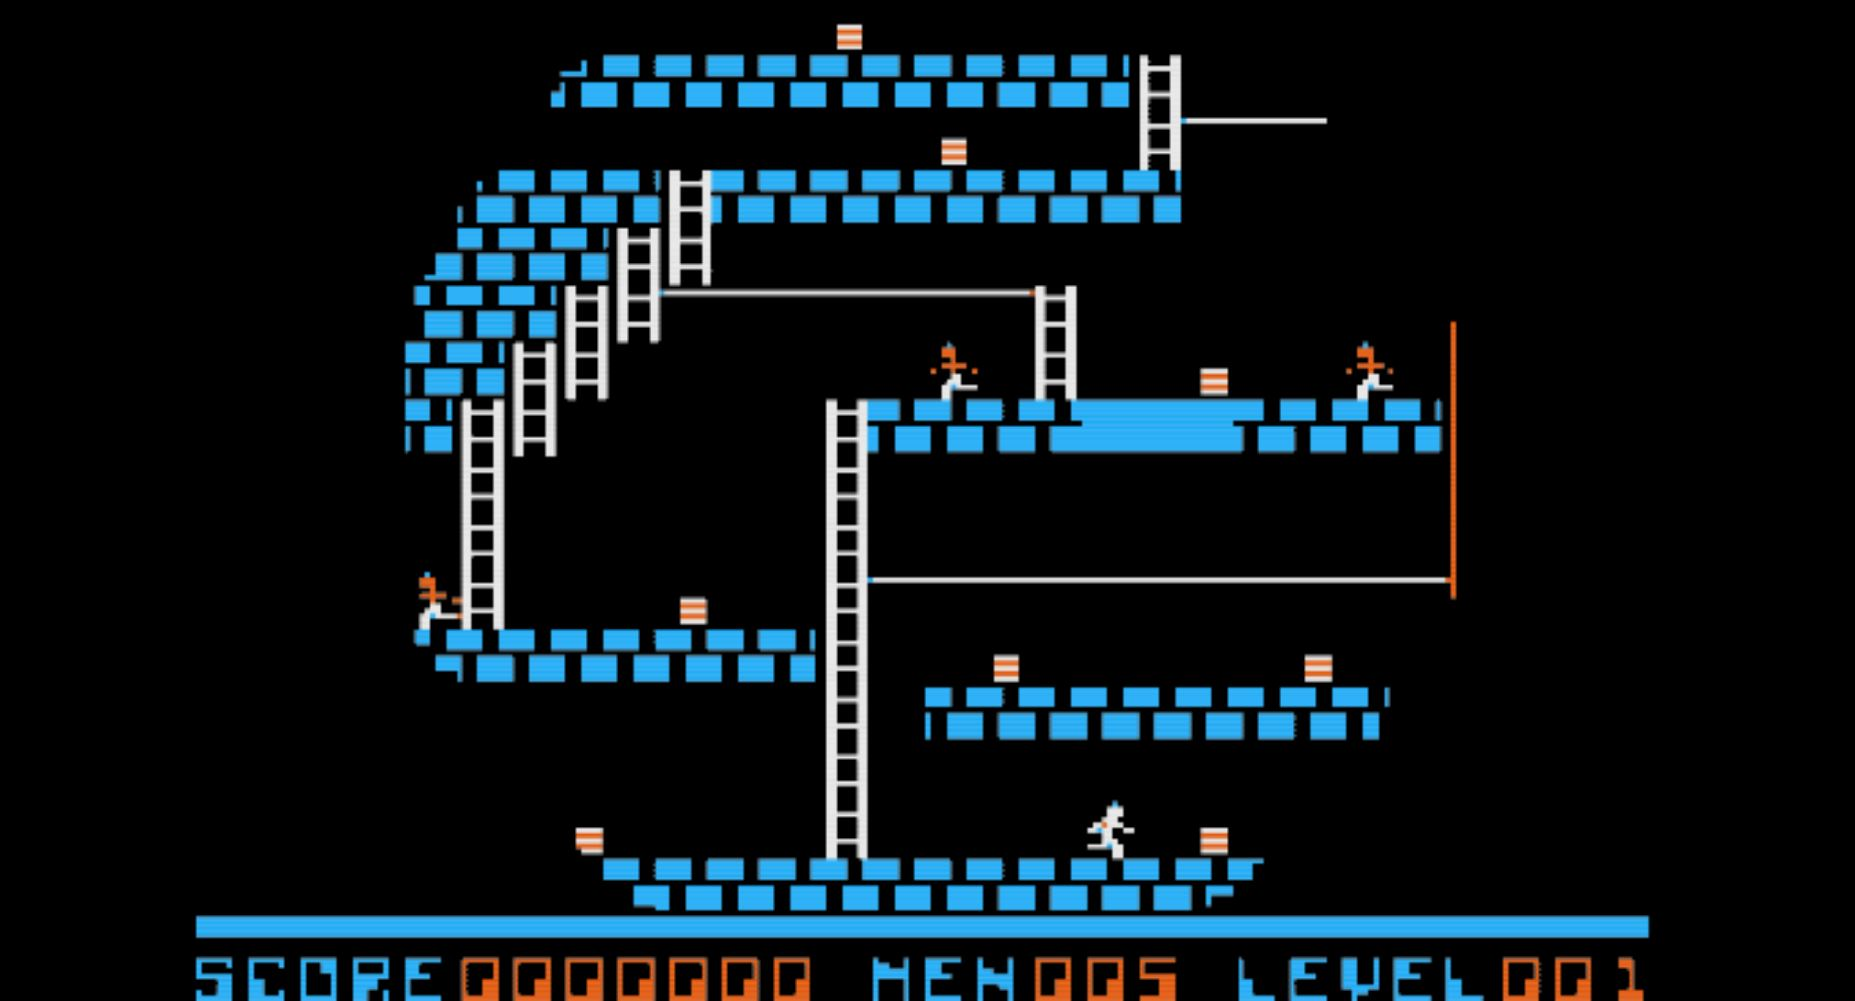
\includegraphics[width=\columnwidth]{iris}

\nwenddocs{}\nwbegincode{208}\sublabel{NW1Xx3lK-10jlgu-Q}\nwmargintag{{\nwtagstyle{}\subpageref{NW1Xx3lK-10jlgu-Q}}}\moddef{defines~{\nwtagstyle{}\subpageref{NW1Xx3lK-10jlgu-1}}}\plusendmoddef\nwstartdeflinemarkup\nwusesondefline{\\{NW1Xx3lK-1p0Y9w-1}}\nwprevnextdefs{NW1Xx3lK-10jlgu-P}{NW1Xx3lK-10jlgu-R}\nwenddeflinemarkup
\nwlinkedidentc{WIPE_COUNTER}{NW1Xx3lK-10jlgu-Q}        EQU     $6D
\nwlinkedidentc{WIPE_MODE}{NW1Xx3lK-10jlgu-Q}           EQU     $A5     ; 0 for open, 1 for close.
WIPE_DIR            EQU     $72     ; 0 for close, 1 for open.
WIPE_CENTER_X       EQU     $74
WIPE_CENTER_Y       EQU     $73
\nwindexdefn{\nwixident{WIPE{\_}COUNTER}}{WIPE:unCOUNTER}{NW1Xx3lK-10jlgu-Q}\nwindexdefn{\nwixident{WIPE{\_}MODE}}{WIPE:unMODE}{NW1Xx3lK-10jlgu-Q}\eatline
\nwused{\\{NW1Xx3lK-1p0Y9w-1}}\nwidentdefs{\\{{\nwixident{WIPE{\_}COUNTER}}{WIPE:unCOUNTER}}\\{{\nwixident{WIPE{\_}MODE}}{WIPE:unMODE}}}\nwendcode{}\nwbegindocs{209}\nwdocspar
\nwenddocs{}\nwbegincode{210}\sublabel{NW1Xx3lK-6p0m3-1}\nwmargintag{{\nwtagstyle{}\subpageref{NW1Xx3lK-6p0m3-1}}}\moddef{iris wipe~{\nwtagstyle{}\subpageref{NW1Xx3lK-6p0m3-1}}}\endmoddef\nwstartdeflinemarkup\nwusesondefline{\\{NW1Xx3lK-8jv1b-C}}\nwenddeflinemarkup
    ORG     $88A2
\nwlinkedidentc{IRIS_WIPE}{NW1Xx3lK-6p0m3-1}:
    SUBROUTINE

    LDA     #88
    STA     WIPE_CENTER_Y
    LDA     #140
    STA     WIPE_CENTER_X

    LDA     \nwlinkedidentc{WIPE_MODE}{NW1Xx3lK-10jlgu-Q}
    BEQ     .iris_open

    LDX     #$AA
    STX     \nwlinkedidentc{WIPE_COUNTER}{NW1Xx3lK-10jlgu-Q}
    LDX     #$00
    STX     WIPE_DIR             ; Close

.loop_close:
    JSR     \nwlinkedidentc{IRIS_WIPE_STEP}{NW1Xx3lK-1tGalf-1}
    DEC     \nwlinkedidentc{WIPE_COUNTER}{NW1Xx3lK-10jlgu-Q}
    BNE     .loop_close

.iris_open:
    LDA     #$01
    STA     \nwlinkedidentc{WIPE_COUNTER}{NW1Xx3lK-10jlgu-Q}
    STA     \nwlinkedidentc{WIPE_MODE}{NW1Xx3lK-10jlgu-Q}           ; So next time we will close.
    STA     WIPE_DIR            ; Open
    JSR     \nwlinkedidentc{PUT_STATUS_LIVES}{NW1Xx3lK-458dZ9-1}
    JSR     \nwlinkedidentc{PUT_STATUS_LEVEL}{NW1Xx3lK-458dZ9-1}

.loop_open:
    JSR     \nwlinkedidentc{IRIS_WIPE_STEP}{NW1Xx3lK-1tGalf-1}
    INC     \nwlinkedidentc{WIPE_COUNTER}{NW1Xx3lK-10jlgu-Q}
    LDA     \nwlinkedidentc{WIPE_COUNTER}{NW1Xx3lK-10jlgu-Q}
    CMP     #$AA
    BNE     .loop_open
    RTS
\nwindexdefn{\nwixident{IRIS{\_}WIPE}}{IRIS:unWIPE}{NW1Xx3lK-6p0m3-1}\eatline
\nwused{\\{NW1Xx3lK-8jv1b-C}}\nwidentdefs{\\{{\nwixident{IRIS{\_}WIPE}}{IRIS:unWIPE}}}\nwidentuses{\\{{\nwixident{IRIS{\_}WIPE{\_}STEP}}{IRIS:unWIPE:unSTEP}}\\{{\nwixident{PUT{\_}STATUS{\_}LEVEL}}{PUT:unSTATUS:unLEVEL}}\\{{\nwixident{PUT{\_}STATUS{\_}LIVES}}{PUT:unSTATUS:unLIVES}}\\{{\nwixident{WIPE{\_}COUNTER}}{WIPE:unCOUNTER}}\\{{\nwixident{WIPE{\_}MODE}}{WIPE:unMODE}}}\nwindexuse{\nwixident{IRIS{\_}WIPE{\_}STEP}}{IRIS:unWIPE:unSTEP}{NW1Xx3lK-6p0m3-1}\nwindexuse{\nwixident{PUT{\_}STATUS{\_}LEVEL}}{PUT:unSTATUS:unLEVEL}{NW1Xx3lK-6p0m3-1}\nwindexuse{\nwixident{PUT{\_}STATUS{\_}LIVES}}{PUT:unSTATUS:unLIVES}{NW1Xx3lK-6p0m3-1}\nwindexuse{\nwixident{WIPE{\_}COUNTER}}{WIPE:unCOUNTER}{NW1Xx3lK-6p0m3-1}\nwindexuse{\nwixident{WIPE{\_}MODE}}{WIPE:unMODE}{NW1Xx3lK-6p0m3-1}\nwendcode{}\nwbegindocs{211}\nwdocspar
The routine {\Tt{}\nwlinkedidentq{IRIS{\_}WIPE{\_}STEP}{NW1Xx3lK-1tGalf-1}\nwendquote} does a lot of math to compute the circular iris, all parameterized
on {\Tt{}\nwlinkedidentq{WIPE{\_}COUNTER}{NW1Xx3lK-10jlgu-Q}\nwendquote}.

Here is a routine that divides a 16-bit value in A and X (X being LSB) by 7, storing the
result in Y, with remainder in A. The routine effectively does long division. It also uses two temporaries.

\nwenddocs{}\nwbegincode{212}\sublabel{NW1Xx3lK-8jv1b-B}\nwmargintag{{\nwtagstyle{}\subpageref{NW1Xx3lK-8jv1b-B}}}\moddef{routines~{\nwtagstyle{}\subpageref{NW1Xx3lK-8jv1b-1}}}\plusendmoddef\nwstartdeflinemarkup\nwusesondefline{\\{NW1Xx3lK-1p0Y9w-1}}\nwprevnextdefs{NW1Xx3lK-8jv1b-A}{NW1Xx3lK-8jv1b-C}\nwenddeflinemarkup
    ORG     $8A45
\nwlinkedidentc{DIV_BY_7}{NW1Xx3lK-8jv1b-B}:
    SUBROUTINE
    ; Enter routine with AX set to (unsigned) numerator.
    ; On exit, Y will contain the integer portion of AX/7,
    ; and A contains the remainder.

    STX     \nwlinkedidentc{MATH_TMPL}{NW1Xx3lK-10jlgu-1}
    LDY     #$08
    SEC
    SBC     #$07

.loop:
    PHP
    ROL     \nwlinkedidentc{MATH_TMPH}{NW1Xx3lK-10jlgu-1}
    ASL     \nwlinkedidentc{MATH_TMPL}{NW1Xx3lK-10jlgu-1}
    ROL
    PLP
    BCC     .adjust_up
    SBC     #$07
    JMP     .next

.adjust_up
    ADC     #$07

.next
    DEY
    BNE     .loop

    BCS     .no_adjust
    ADC     #$07
    CLC

.no_adjust
    ROL     \nwlinkedidentc{MATH_TMPH}{NW1Xx3lK-10jlgu-1}
    LDY     \nwlinkedidentc{MATH_TMPH}{NW1Xx3lK-10jlgu-1}
    RTS
\nwindexdefn{\nwixident{DIV{\_}BY{\_}7}}{DIV:unBY:un7}{NW1Xx3lK-8jv1b-B}\eatline
\nwused{\\{NW1Xx3lK-1p0Y9w-1}}\nwidentdefs{\\{{\nwixident{DIV{\_}BY{\_}7}}{DIV:unBY:un7}}}\nwidentuses{\\{{\nwixident{MATH{\_}TMPH}}{MATH:unTMPH}}\\{{\nwixident{MATH{\_}TMPL}}{MATH:unTMPL}}}\nwindexuse{\nwixident{MATH{\_}TMPH}}{MATH:unTMPH}{NW1Xx3lK-8jv1b-B}\nwindexuse{\nwixident{MATH{\_}TMPL}}{MATH:unTMPL}{NW1Xx3lK-8jv1b-B}\nwendcode{}\nwbegindocs{213}\nwdocspar
Now, for one iris wipe step, we will need lots and lots of temporaries.

\nwenddocs{}\nwbegincode{214}\sublabel{NW1Xx3lK-10jlgu-R}\nwmargintag{{\nwtagstyle{}\subpageref{NW1Xx3lK-10jlgu-R}}}\moddef{defines~{\nwtagstyle{}\subpageref{NW1Xx3lK-10jlgu-1}}}\plusendmoddef\nwstartdeflinemarkup\nwusesondefline{\\{NW1Xx3lK-1p0Y9w-1}}\nwprevnextdefs{NW1Xx3lK-10jlgu-Q}{NW1Xx3lK-10jlgu-S}\nwenddeflinemarkup
\nwlinkedidentc{WIPE0}{NW1Xx3lK-10jlgu-R}       EQU     $69     ; 16-bit value
\nwlinkedidentc{WIPE1}{NW1Xx3lK-10jlgu-R}       EQU     $67     ; 16-bit value
\nwlinkedidentc{WIPE2}{NW1Xx3lK-10jlgu-R}       EQU     $6B     ; 16-bit value
\nwlinkedidentc{WIPE3L}{NW1Xx3lK-10jlgu-R}      EQU     $75
\nwlinkedidentc{WIPE4L}{NW1Xx3lK-10jlgu-R}      EQU     $76
\nwlinkedidentc{WIPE5L}{NW1Xx3lK-10jlgu-R}      EQU     $77
\nwlinkedidentc{WIPE6L}{NW1Xx3lK-10jlgu-R}      EQU     $78
\nwlinkedidentc{WIPE3H}{NW1Xx3lK-10jlgu-R}      EQU     $79
\nwlinkedidentc{WIPE4H}{NW1Xx3lK-10jlgu-R}      EQU     $7A
\nwlinkedidentc{WIPE5H}{NW1Xx3lK-10jlgu-R}      EQU     $7B
\nwlinkedidentc{WIPE6H}{NW1Xx3lK-10jlgu-R}      EQU     $7C
\nwlinkedidentc{WIPE7D}{NW1Xx3lK-10jlgu-R}      EQU     $7D     ; Dividends
\nwlinkedidentc{WIPE8D}{NW1Xx3lK-10jlgu-R}      EQU     $7E
\nwlinkedidentc{WIPE9D}{NW1Xx3lK-10jlgu-R}      EQU     $7F
\nwlinkedidentc{WIPE10D}{NW1Xx3lK-10jlgu-R}     EQU     $80
\nwlinkedidentc{WIPE7R}{NW1Xx3lK-10jlgu-R}      EQU     $81     ; Remainders
\nwlinkedidentc{WIPE8R}{NW1Xx3lK-10jlgu-R}      EQU     $82
\nwlinkedidentc{WIPE9R}{NW1Xx3lK-10jlgu-R}      EQU     $83
\nwlinkedidentc{WIPE10R}{NW1Xx3lK-10jlgu-R}     EQU     $84
\nwindexdefn{\nwixident{WIPE0}}{WIPE0}{NW1Xx3lK-10jlgu-R}\nwindexdefn{\nwixident{WIPE1}}{WIPE1}{NW1Xx3lK-10jlgu-R}\nwindexdefn{\nwixident{WIPE2}}{WIPE2}{NW1Xx3lK-10jlgu-R}\nwindexdefn{\nwixident{WIPE3L}}{WIPE3L}{NW1Xx3lK-10jlgu-R}\nwindexdefn{\nwixident{WIPE3H}}{WIPE3H}{NW1Xx3lK-10jlgu-R}\nwindexdefn{\nwixident{WIPE4L}}{WIPE4L}{NW1Xx3lK-10jlgu-R}\nwindexdefn{\nwixident{WIPE4H}}{WIPE4H}{NW1Xx3lK-10jlgu-R}\nwindexdefn{\nwixident{WIPE5L}}{WIPE5L}{NW1Xx3lK-10jlgu-R}\nwindexdefn{\nwixident{WIPE5H}}{WIPE5H}{NW1Xx3lK-10jlgu-R}\nwindexdefn{\nwixident{WIPE6L}}{WIPE6L}{NW1Xx3lK-10jlgu-R}\nwindexdefn{\nwixident{WIPE6H}}{WIPE6H}{NW1Xx3lK-10jlgu-R}\nwindexdefn{\nwixident{WIPE7D}}{WIPE7D}{NW1Xx3lK-10jlgu-R}\nwindexdefn{\nwixident{WIPE7R}}{WIPE7R}{NW1Xx3lK-10jlgu-R}\nwindexdefn{\nwixident{WIPE8D}}{WIPE8D}{NW1Xx3lK-10jlgu-R}\nwindexdefn{\nwixident{WIPE8R}}{WIPE8R}{NW1Xx3lK-10jlgu-R}\nwindexdefn{\nwixident{WIPE9D}}{WIPE9D}{NW1Xx3lK-10jlgu-R}\nwindexdefn{\nwixident{WIPE9R}}{WIPE9R}{NW1Xx3lK-10jlgu-R}\nwindexdefn{\nwixident{WIPE10D}}{WIPE10D}{NW1Xx3lK-10jlgu-R}\nwindexdefn{\nwixident{WIPE10R}}{WIPE10R}{NW1Xx3lK-10jlgu-R}\eatline
\nwused{\\{NW1Xx3lK-1p0Y9w-1}}\nwidentdefs{\\{{\nwixident{WIPE0}}{WIPE0}}\\{{\nwixident{WIPE1}}{WIPE1}}\\{{\nwixident{WIPE10D}}{WIPE10D}}\\{{\nwixident{WIPE10R}}{WIPE10R}}\\{{\nwixident{WIPE2}}{WIPE2}}\\{{\nwixident{WIPE3H}}{WIPE3H}}\\{{\nwixident{WIPE3L}}{WIPE3L}}\\{{\nwixident{WIPE4H}}{WIPE4H}}\\{{\nwixident{WIPE4L}}{WIPE4L}}\\{{\nwixident{WIPE5H}}{WIPE5H}}\\{{\nwixident{WIPE5L}}{WIPE5L}}\\{{\nwixident{WIPE6H}}{WIPE6H}}\\{{\nwixident{WIPE6L}}{WIPE6L}}\\{{\nwixident{WIPE7D}}{WIPE7D}}\\{{\nwixident{WIPE7R}}{WIPE7R}}\\{{\nwixident{WIPE8D}}{WIPE8D}}\\{{\nwixident{WIPE8R}}{WIPE8R}}\\{{\nwixident{WIPE9D}}{WIPE9D}}\\{{\nwixident{WIPE9R}}{WIPE9R}}}\nwendcode{}\nwbegindocs{215}\nwdocspar
The first thing we do for a single step is initialize all those variables!

\nwenddocs{}\nwbegincode{216}\sublabel{NW1Xx3lK-1tGalf-1}\nwmargintag{{\nwtagstyle{}\subpageref{NW1Xx3lK-1tGalf-1}}}\moddef{iris wipe step~{\nwtagstyle{}\subpageref{NW1Xx3lK-1tGalf-1}}}\endmoddef\nwstartdeflinemarkup\nwusesondefline{\\{NW1Xx3lK-8jv1b-C}}\nwprevnextdefs{\relax}{NW1Xx3lK-1tGalf-2}\nwenddeflinemarkup
    ORG     $88D7
\nwlinkedidentc{IRIS_WIPE_STEP}{NW1Xx3lK-1tGalf-1}:
    SUBROUTINE

\LA{}\code{}WIPE0\ =\ WIPE{\_}COUNTER\edoc{}~{\nwtagstyle{}\subpageref{NW1Xx3lK-2Rx43B-1}}\RA{}
\LA{}\code{}WIPE1\ =\ 0\edoc{}~{\nwtagstyle{}\subpageref{NW1Xx3lK-1ZlBVV-1}}\RA{}
\LA{}\code{}WIPE2\ =\ 2\ *\ WIPE0\edoc{}~{\nwtagstyle{}\subpageref{NW1Xx3lK-39zOBY-1}}\RA{}
\LA{}\code{}WIPE2\ =\ 3\ -\ WIPE2\edoc{}~{\nwtagstyle{}\subpageref{NW1Xx3lK-1Ny5Ce-1}}\RA{}

; WIPE3, WIPE4, WIPE5, and WIPE6 correspond to
; row numbers. WIPE3 is above the center, WIPE6
; is below the center, while WIPE4 and WIPE5 are on
; the center.

\LA{}\code{}WIPE3\ =\ WIPE{\_}CENTER{\_}Y\ -\ WIPE{\_}COUNTER\edoc{}~{\nwtagstyle{}\subpageref{NW1Xx3lK-3R5hBF-1}}\RA{}
\LA{}\code{}WIPE4\ =\ WIPE5\ =\ WIPE{\_}CENTER{\_}Y\edoc{}~{\nwtagstyle{}\subpageref{NW1Xx3lK-2JOPWw-1}}\RA{}
\LA{}\code{}WIPE6\ =\ WIPE{\_}CENTER{\_}Y\ +\ WIPE{\_}COUNTER\edoc{}~{\nwtagstyle{}\subpageref{NW1Xx3lK-4TkslJ-1}}\RA{}

; WIPE7, WIPE8, WIPE9, and WIPE10 correspond to
; column byte numbers. Note the division by 7 pixels!
; WIPE7 is left of center, WIPE10 is right of center,
; while WIPE8 and WIPE9 are on the center.

\LA{}\code{}WIPE7\ =\ (WIPE{\_}CENTER{\_}X\ -\ WIPE{\_}COUNTER)\ /\ 7\edoc{}~{\nwtagstyle{}\subpageref{NW1Xx3lK-2ojStX-1}}\RA{}
\LA{}\code{}WIPE8\ =\ WIPE9\ =\ WIPE{\_}CENTER{\_}X\ /\ 7\edoc{}~{\nwtagstyle{}\subpageref{NW1Xx3lK-2QGdSi-1}}\RA{}
\LA{}\code{}WIPE10\ =\ (WIPE{\_}CENTER{\_}X\ +\ WIPE{\_}COUNTER)\ /\ 7\edoc{}~{\nwtagstyle{}\subpageref{NW1Xx3lK-2Um1dk-1}}\RA{}
\nwindexdefn{\nwixident{IRIS{\_}WIPE{\_}STEP}}{IRIS:unWIPE:unSTEP}{NW1Xx3lK-1tGalf-1}\eatline
\nwalsodefined{\\{NW1Xx3lK-1tGalf-2}}\nwused{\\{NW1Xx3lK-8jv1b-C}}\nwidentdefs{\\{{\nwixident{IRIS{\_}WIPE{\_}STEP}}{IRIS:unWIPE:unSTEP}}}\nwendcode{}\nwbegindocs{217}\nwdocspar
Now we loop. This involves checking {\Tt{}\nwlinkedidentq{WIPE1}{NW1Xx3lK-10jlgu-R}\nwendquote} against {\Tt{}\nwlinkedidentq{WIPE0}{NW1Xx3lK-10jlgu-R}\nwendquote}:

\begin{itemize}
  \item If {\Tt{}\nwlinkedidentq{WIPE1}{NW1Xx3lK-10jlgu-R}\nwendquote} $<$ {\Tt{}\nwlinkedidentq{WIPE0}{NW1Xx3lK-10jlgu-R}\nwendquote}, return.
  \item If {\Tt{}\nwlinkedidentq{WIPE1}{NW1Xx3lK-10jlgu-R}\nwendquote} == {\Tt{}\nwlinkedidentq{WIPE0}{NW1Xx3lK-10jlgu-R}\nwendquote}, go to {\Tt{}\nwlinkedidentq{DRAW{\_}WIPE{\_}STEP}{NW1Xx3lK-1DtO18-1}\nwendquote} then return.
  \item Otherwise, call {\Tt{}\nwlinkedidentq{DRAW{\_}WIPE{\_}STEP}{NW1Xx3lK-1DtO18-1}\nwendquote} and go round the loop.
\end{itemize}

Going around the loop involves calling {\Tt{}\nwlinkedidentq{DRAW{\_}WIPE{\_}STEP}{NW1Xx3lK-1DtO18-1}\nwendquote}, then adjusting
the numbers.

\nwenddocs{}\nwbegincode{218}\sublabel{NW1Xx3lK-1tGalf-2}\nwmargintag{{\nwtagstyle{}\subpageref{NW1Xx3lK-1tGalf-2}}}\moddef{iris wipe step~{\nwtagstyle{}\subpageref{NW1Xx3lK-1tGalf-1}}}\plusendmoddef\nwstartdeflinemarkup\nwusesondefline{\\{NW1Xx3lK-8jv1b-C}}\nwprevnextdefs{NW1Xx3lK-1tGalf-1}{\relax}\nwenddeflinemarkup
.loop:

\LA{}iris wipe loop check~{\nwtagstyle{}\subpageref{NW1Xx3lK-3vxyMm-1}}\RA{}

    JSR     \nwlinkedidentc{DRAW_WIPE_STEP}{NW1Xx3lK-1DtO18-1}

    LDA     \nwlinkedidentc{WIPE2}{NW1Xx3lK-10jlgu-R}+1
    BPL     .89a7

\LA{}\code{}WIPE2\ +=\ 4\ *\ WIPE1\ +\ 6\edoc{}~{\nwtagstyle{}\subpageref{NW1Xx3lK-mcL2B-1}}\RA{}
    JMP     .8a14

.89a7:

\LA{}\code{}WIPE2\ +=\ 4\ *\ (WIPE1\ -\ WIPE0)\ +\ 16\edoc{}~{\nwtagstyle{}\subpageref{NW1Xx3lK-2eL1Rw-1}}\RA{}
\LA{}Decrement \code{}WIPE0\edoc{}~{\nwtagstyle{}\subpageref{NW1Xx3lK-2u2rZr-1}}\RA{}
\LA{}Increment \code{}WIPE3\edoc{}~{\nwtagstyle{}\subpageref{NW1Xx3lK-13RMM3-1}}\RA{}
\LA{}Decrement \code{}WIPE10\edoc{} modulo 7~{\nwtagstyle{}\subpageref{NW1Xx3lK-11REH7-1}}\RA{}
\LA{}Increment \code{}WIPE7\edoc{} modulo 7~{\nwtagstyle{}\subpageref{NW1Xx3lK-11uG8h-1}}\RA{}
\LA{}Decrement \code{}WIPE6\edoc{}~{\nwtagstyle{}\subpageref{NW1Xx3lK-2u2n6B-1}}\RA{}

.8a14:

\LA{}Increment \code{}WIPE1\edoc{}~{\nwtagstyle{}\subpageref{NW1Xx3lK-13RECF-1}}\RA{}
\LA{}Increment \code{}WIPE9\edoc{} modulo 7~{\nwtagstyle{}\subpageref{NW1Xx3lK-3Y2gMs-1}}\RA{}
\LA{}Decrement \code{}WIPE4\edoc{}~{\nwtagstyle{}\subpageref{NW1Xx3lK-2u2srL-1}}\RA{}
\LA{}Increment \code{}WIPE5\edoc{}~{\nwtagstyle{}\subpageref{NW1Xx3lK-13RI6p-1}}\RA{}
\LA{}Decrement \code{}WIPE8\edoc{} modulo 7~{\nwtagstyle{}\subpageref{NW1Xx3lK-nzt1T-1}}\RA{}
    JMP     .loop
\nwused{\\{NW1Xx3lK-8jv1b-C}}\nwidentuses{\\{{\nwixident{DRAW{\_}WIPE{\_}STEP}}{DRAW:unWIPE:unSTEP}}\\{{\nwixident{WIPE2}}{WIPE2}}}\nwindexuse{\nwixident{DRAW{\_}WIPE{\_}STEP}}{DRAW:unWIPE:unSTEP}{NW1Xx3lK-1tGalf-2}\nwindexuse{\nwixident{WIPE2}}{WIPE2}{NW1Xx3lK-1tGalf-2}\nwendcode{}\nwbegindocs{219}\nwdocspar

Drawing a wipe step draws all four parts. There are two rows which move north
and two rows that move south. There are also two left and right offsets, one
short and one long. This makes eight combinations.

\nwenddocs{}\nwbegincode{220}\sublabel{NW1Xx3lK-1DtO18-1}\nwmargintag{{\nwtagstyle{}\subpageref{NW1Xx3lK-1DtO18-1}}}\moddef{draw wipe step~{\nwtagstyle{}\subpageref{NW1Xx3lK-1DtO18-1}}}\endmoddef\nwstartdeflinemarkup\nwusesondefline{\\{NW1Xx3lK-8jv1b-C}}\nwenddeflinemarkup
    ORG     $8A69
\nwlinkedidentc{DRAW_WIPE_STEP}{NW1Xx3lK-1DtO18-1}:
    SUBROUTINE

\LA{}Draw wipe for south part~{\nwtagstyle{}\subpageref{NW1Xx3lK-29jG99-1}}\RA{}
\LA{}Draw wipe for north part~{\nwtagstyle{}\subpageref{NW1Xx3lK-29yoMR-1}}\RA{}
\LA{}Draw wipe for north2 part~{\nwtagstyle{}\subpageref{NW1Xx3lK-3AjGdu-1}}\RA{}
\LA{}Draw wipe for south2 part~{\nwtagstyle{}\subpageref{NW1Xx3lK-3OCJye-1}}\RA{}
\nwindexdefn{\nwixident{DRAW{\_}WIPE{\_}STEP}}{DRAW:unWIPE:unSTEP}{NW1Xx3lK-1DtO18-1}\eatline
\nwused{\\{NW1Xx3lK-8jv1b-C}}\nwidentdefs{\\{{\nwixident{DRAW{\_}WIPE{\_}STEP}}{DRAW:unWIPE:unSTEP}}}\nwendcode{}\nwbegindocs{221}\nwdocspar
Each part consists of two halves, right and left (or east and west).

\nwenddocs{}\nwbegincode{222}\sublabel{NW1Xx3lK-29jG99-1}\nwmargintag{{\nwtagstyle{}\subpageref{NW1Xx3lK-29jG99-1}}}\moddef{Draw wipe for south part~{\nwtagstyle{}\subpageref{NW1Xx3lK-29jG99-1}}}\endmoddef\nwstartdeflinemarkup\nwusesondefline{\\{NW1Xx3lK-1DtO18-1}}\nwenddeflinemarkup
    LDY     \nwlinkedidentc{WIPE6H}{NW1Xx3lK-10jlgu-R}
    BNE     .draw_north
    LDY     \nwlinkedidentc{WIPE6L}{NW1Xx3lK-10jlgu-R}
    CPY     #176
    BCS     .draw_north        ; Skip if WIPE6 >= 176

    JSR     \nwlinkedidentc{ROW_TO_ADDR_FOR_BOTH_PAGES}{NW1Xx3lK-8jv1b-4}

    ; East side
    LDY     \nwlinkedidentc{WIPE9D}{NW1Xx3lK-10jlgu-R}
    CPY     #40
    BCS     .draw_south_west
    LDX     \nwlinkedidentc{WIPE9R}{NW1Xx3lK-10jlgu-R}
    JSR     \nwlinkedidentc{DRAW_WIPE_BLOCK}{NW1Xx3lK-32wUsj-1}

.draw_south_west
    ; West side
    LDY     \nwlinkedidentc{WIPE8D}{NW1Xx3lK-10jlgu-R}
    CPY     #40
    BCS     .draw_north
    LDX     \nwlinkedidentc{WIPE8R}{NW1Xx3lK-10jlgu-R}
    JSR     \nwlinkedidentc{DRAW_WIPE_BLOCK}{NW1Xx3lK-32wUsj-1}
\nwused{\\{NW1Xx3lK-1DtO18-1}}\nwidentuses{\\{{\nwixident{DRAW{\_}WIPE{\_}BLOCK}}{DRAW:unWIPE:unBLOCK}}\\{{\nwixident{ROW{\_}TO{\_}ADDR{\_}FOR{\_}BOTH{\_}PAGES}}{ROW:unTO:unADDR:unFOR:unBOTH:unPAGES}}\\{{\nwixident{WIPE6H}}{WIPE6H}}\\{{\nwixident{WIPE6L}}{WIPE6L}}\\{{\nwixident{WIPE8D}}{WIPE8D}}\\{{\nwixident{WIPE8R}}{WIPE8R}}\\{{\nwixident{WIPE9D}}{WIPE9D}}\\{{\nwixident{WIPE9R}}{WIPE9R}}}\nwindexuse{\nwixident{DRAW{\_}WIPE{\_}BLOCK}}{DRAW:unWIPE:unBLOCK}{NW1Xx3lK-29jG99-1}\nwindexuse{\nwixident{ROW{\_}TO{\_}ADDR{\_}FOR{\_}BOTH{\_}PAGES}}{ROW:unTO:unADDR:unFOR:unBOTH:unPAGES}{NW1Xx3lK-29jG99-1}\nwindexuse{\nwixident{WIPE6H}}{WIPE6H}{NW1Xx3lK-29jG99-1}\nwindexuse{\nwixident{WIPE6L}}{WIPE6L}{NW1Xx3lK-29jG99-1}\nwindexuse{\nwixident{WIPE8D}}{WIPE8D}{NW1Xx3lK-29jG99-1}\nwindexuse{\nwixident{WIPE8R}}{WIPE8R}{NW1Xx3lK-29jG99-1}\nwindexuse{\nwixident{WIPE9D}}{WIPE9D}{NW1Xx3lK-29jG99-1}\nwindexuse{\nwixident{WIPE9R}}{WIPE9R}{NW1Xx3lK-29jG99-1}\nwendcode{}\nwbegindocs{223}\nwdocspar

\nwenddocs{}\nwbegincode{224}\sublabel{NW1Xx3lK-29yoMR-1}\nwmargintag{{\nwtagstyle{}\subpageref{NW1Xx3lK-29yoMR-1}}}\moddef{Draw wipe for north part~{\nwtagstyle{}\subpageref{NW1Xx3lK-29yoMR-1}}}\endmoddef\nwstartdeflinemarkup\nwusesondefline{\\{NW1Xx3lK-1DtO18-1}}\nwenddeflinemarkup
.draw_north:
    LDY     \nwlinkedidentc{WIPE3H}{NW1Xx3lK-10jlgu-R}
    BNE     .draw_north2
    LDY     \nwlinkedidentc{WIPE3L}{NW1Xx3lK-10jlgu-R}
    CPY     #176
    BCS     .draw_north2        ; Skip if WIPE3 >= 176

    JSR     \nwlinkedidentc{ROW_TO_ADDR_FOR_BOTH_PAGES}{NW1Xx3lK-8jv1b-4}

    ; East side
    LDY     \nwlinkedidentc{WIPE9D}{NW1Xx3lK-10jlgu-R}
    CPY     #40
    BCS     .draw_north_west
    LDX     \nwlinkedidentc{WIPE9R}{NW1Xx3lK-10jlgu-R}
    JSR     \nwlinkedidentc{DRAW_WIPE_BLOCK}{NW1Xx3lK-32wUsj-1}

.draw_north_west
    ; West side
    LDY     \nwlinkedidentc{WIPE8D}{NW1Xx3lK-10jlgu-R}
    CPY     #40
    BCS     .draw_north2
    LDX     \nwlinkedidentc{WIPE8R}{NW1Xx3lK-10jlgu-R}
    JSR     \nwlinkedidentc{DRAW_WIPE_BLOCK}{NW1Xx3lK-32wUsj-1}
\nwused{\\{NW1Xx3lK-1DtO18-1}}\nwidentuses{\\{{\nwixident{DRAW{\_}WIPE{\_}BLOCK}}{DRAW:unWIPE:unBLOCK}}\\{{\nwixident{ROW{\_}TO{\_}ADDR{\_}FOR{\_}BOTH{\_}PAGES}}{ROW:unTO:unADDR:unFOR:unBOTH:unPAGES}}\\{{\nwixident{WIPE3H}}{WIPE3H}}\\{{\nwixident{WIPE3L}}{WIPE3L}}\\{{\nwixident{WIPE8D}}{WIPE8D}}\\{{\nwixident{WIPE8R}}{WIPE8R}}\\{{\nwixident{WIPE9D}}{WIPE9D}}\\{{\nwixident{WIPE9R}}{WIPE9R}}}\nwindexuse{\nwixident{DRAW{\_}WIPE{\_}BLOCK}}{DRAW:unWIPE:unBLOCK}{NW1Xx3lK-29yoMR-1}\nwindexuse{\nwixident{ROW{\_}TO{\_}ADDR{\_}FOR{\_}BOTH{\_}PAGES}}{ROW:unTO:unADDR:unFOR:unBOTH:unPAGES}{NW1Xx3lK-29yoMR-1}\nwindexuse{\nwixident{WIPE3H}}{WIPE3H}{NW1Xx3lK-29yoMR-1}\nwindexuse{\nwixident{WIPE3L}}{WIPE3L}{NW1Xx3lK-29yoMR-1}\nwindexuse{\nwixident{WIPE8D}}{WIPE8D}{NW1Xx3lK-29yoMR-1}\nwindexuse{\nwixident{WIPE8R}}{WIPE8R}{NW1Xx3lK-29yoMR-1}\nwindexuse{\nwixident{WIPE9D}}{WIPE9D}{NW1Xx3lK-29yoMR-1}\nwindexuse{\nwixident{WIPE9R}}{WIPE9R}{NW1Xx3lK-29yoMR-1}\nwendcode{}\nwbegindocs{225}\nwdocspar

\nwenddocs{}\nwbegincode{226}\sublabel{NW1Xx3lK-3AjGdu-1}\nwmargintag{{\nwtagstyle{}\subpageref{NW1Xx3lK-3AjGdu-1}}}\moddef{Draw wipe for north2 part~{\nwtagstyle{}\subpageref{NW1Xx3lK-3AjGdu-1}}}\endmoddef\nwstartdeflinemarkup\nwusesondefline{\\{NW1Xx3lK-1DtO18-1}}\nwenddeflinemarkup
.draw_north2:
    LDY     \nwlinkedidentc{WIPE5H}{NW1Xx3lK-10jlgu-R}
    BNE     .draw_south2
    LDY     \nwlinkedidentc{WIPE5L}{NW1Xx3lK-10jlgu-R}
    CPY     #176
    BCS     .draw_south2        ; Skip if WIPE5 >= 176

    JSR     \nwlinkedidentc{ROW_TO_ADDR_FOR_BOTH_PAGES}{NW1Xx3lK-8jv1b-4}

    ; East side
    LDY     \nwlinkedidentc{WIPE10D}{NW1Xx3lK-10jlgu-R}
    CPY     #40
    BCS     .draw_north2_west
    LDX     \nwlinkedidentc{WIPE10R}{NW1Xx3lK-10jlgu-R}
    JSR     \nwlinkedidentc{DRAW_WIPE_BLOCK}{NW1Xx3lK-32wUsj-1}

.draw_north2_west
    ; West side
    LDY     \nwlinkedidentc{WIPE7D}{NW1Xx3lK-10jlgu-R}
    CPY     #40
    BCS     .draw_south2
    LDX     \nwlinkedidentc{WIPE7R}{NW1Xx3lK-10jlgu-R}
    JSR     \nwlinkedidentc{DRAW_WIPE_BLOCK}{NW1Xx3lK-32wUsj-1}
\nwused{\\{NW1Xx3lK-1DtO18-1}}\nwidentuses{\\{{\nwixident{DRAW{\_}WIPE{\_}BLOCK}}{DRAW:unWIPE:unBLOCK}}\\{{\nwixident{ROW{\_}TO{\_}ADDR{\_}FOR{\_}BOTH{\_}PAGES}}{ROW:unTO:unADDR:unFOR:unBOTH:unPAGES}}\\{{\nwixident{WIPE10D}}{WIPE10D}}\\{{\nwixident{WIPE10R}}{WIPE10R}}\\{{\nwixident{WIPE5H}}{WIPE5H}}\\{{\nwixident{WIPE5L}}{WIPE5L}}\\{{\nwixident{WIPE7D}}{WIPE7D}}\\{{\nwixident{WIPE7R}}{WIPE7R}}}\nwindexuse{\nwixident{DRAW{\_}WIPE{\_}BLOCK}}{DRAW:unWIPE:unBLOCK}{NW1Xx3lK-3AjGdu-1}\nwindexuse{\nwixident{ROW{\_}TO{\_}ADDR{\_}FOR{\_}BOTH{\_}PAGES}}{ROW:unTO:unADDR:unFOR:unBOTH:unPAGES}{NW1Xx3lK-3AjGdu-1}\nwindexuse{\nwixident{WIPE10D}}{WIPE10D}{NW1Xx3lK-3AjGdu-1}\nwindexuse{\nwixident{WIPE10R}}{WIPE10R}{NW1Xx3lK-3AjGdu-1}\nwindexuse{\nwixident{WIPE5H}}{WIPE5H}{NW1Xx3lK-3AjGdu-1}\nwindexuse{\nwixident{WIPE5L}}{WIPE5L}{NW1Xx3lK-3AjGdu-1}\nwindexuse{\nwixident{WIPE7D}}{WIPE7D}{NW1Xx3lK-3AjGdu-1}\nwindexuse{\nwixident{WIPE7R}}{WIPE7R}{NW1Xx3lK-3AjGdu-1}\nwendcode{}\nwbegindocs{227}\nwdocspar

\nwenddocs{}\nwbegincode{228}\sublabel{NW1Xx3lK-3OCJye-1}\nwmargintag{{\nwtagstyle{}\subpageref{NW1Xx3lK-3OCJye-1}}}\moddef{Draw wipe for south2 part~{\nwtagstyle{}\subpageref{NW1Xx3lK-3OCJye-1}}}\endmoddef\nwstartdeflinemarkup\nwusesondefline{\\{NW1Xx3lK-1DtO18-1}}\nwenddeflinemarkup
.draw_south2:
    LDY     \nwlinkedidentc{WIPE4H}{NW1Xx3lK-10jlgu-R}
    BNE     .end
    LDY     \nwlinkedidentc{WIPE4L}{NW1Xx3lK-10jlgu-R}
    CPY     #176
    BCS     .end        ; Skip if WIPE4 >= 176

    JSR     \nwlinkedidentc{ROW_TO_ADDR_FOR_BOTH_PAGES}{NW1Xx3lK-8jv1b-4}

    ; East side
    LDY     \nwlinkedidentc{WIPE10D}{NW1Xx3lK-10jlgu-R}
    CPY     #40
    BCS     .draw_south2_west
    LDX     \nwlinkedidentc{WIPE10R}{NW1Xx3lK-10jlgu-R}
    JSR     \nwlinkedidentc{DRAW_WIPE_BLOCK}{NW1Xx3lK-32wUsj-1}

.draw_south2_west
    ; West side
    LDY     \nwlinkedidentc{WIPE7D}{NW1Xx3lK-10jlgu-R}
    CPY     #40
    BCS     .end
    LDX     \nwlinkedidentc{WIPE7R}{NW1Xx3lK-10jlgu-R}
    JMP     \nwlinkedidentc{DRAW_WIPE_BLOCK}{NW1Xx3lK-32wUsj-1}           ; tail call

.end:
    RTS
\nwused{\\{NW1Xx3lK-1DtO18-1}}\nwidentuses{\\{{\nwixident{DRAW{\_}WIPE{\_}BLOCK}}{DRAW:unWIPE:unBLOCK}}\\{{\nwixident{ROW{\_}TO{\_}ADDR{\_}FOR{\_}BOTH{\_}PAGES}}{ROW:unTO:unADDR:unFOR:unBOTH:unPAGES}}\\{{\nwixident{WIPE10D}}{WIPE10D}}\\{{\nwixident{WIPE10R}}{WIPE10R}}\\{{\nwixident{WIPE4H}}{WIPE4H}}\\{{\nwixident{WIPE4L}}{WIPE4L}}\\{{\nwixident{WIPE7D}}{WIPE7D}}\\{{\nwixident{WIPE7R}}{WIPE7R}}}\nwindexuse{\nwixident{DRAW{\_}WIPE{\_}BLOCK}}{DRAW:unWIPE:unBLOCK}{NW1Xx3lK-3OCJye-1}\nwindexuse{\nwixident{ROW{\_}TO{\_}ADDR{\_}FOR{\_}BOTH{\_}PAGES}}{ROW:unTO:unADDR:unFOR:unBOTH:unPAGES}{NW1Xx3lK-3OCJye-1}\nwindexuse{\nwixident{WIPE10D}}{WIPE10D}{NW1Xx3lK-3OCJye-1}\nwindexuse{\nwixident{WIPE10R}}{WIPE10R}{NW1Xx3lK-3OCJye-1}\nwindexuse{\nwixident{WIPE4H}}{WIPE4H}{NW1Xx3lK-3OCJye-1}\nwindexuse{\nwixident{WIPE4L}}{WIPE4L}{NW1Xx3lK-3OCJye-1}\nwindexuse{\nwixident{WIPE7D}}{WIPE7D}{NW1Xx3lK-3OCJye-1}\nwindexuse{\nwixident{WIPE7R}}{WIPE7R}{NW1Xx3lK-3OCJye-1}\nwendcode{}\nwbegindocs{229}\nwdocspar

Drawing a wipe block depends on whether we're opening or closing on the level.
Closing on the level just blacks out pixels on page 1. Opening on the level
copies some pixels from page 2 into page 1.

\nwenddocs{}\nwbegincode{230}\sublabel{NW1Xx3lK-32wUsj-1}\nwmargintag{{\nwtagstyle{}\subpageref{NW1Xx3lK-32wUsj-1}}}\moddef{draw wipe block~{\nwtagstyle{}\subpageref{NW1Xx3lK-32wUsj-1}}}\endmoddef\nwstartdeflinemarkup\nwusesondefline{\\{NW1Xx3lK-8jv1b-C}}\nwenddeflinemarkup
    ORG     $8AF6
\nwlinkedidentc{DRAW_WIPE_BLOCK}{NW1Xx3lK-32wUsj-1}:
    SUBROUTINE
    ; Enter routine with X set to the column byte and Y set to
    ; the pixel number within that byte (0-6). \nwlinkedidentc{ROW_ADDR}{NW1Xx3lK-10jlgu-5} and
    ; \nwlinkedidentc{ROW_ADDR2}{NW1Xx3lK-10jlgu-5} must contain the base row address for page 1
    ; and page 2, respectively.

    LDA     WIPE_DIR
    BNE     .open
    
    LDA     (\nwlinkedidentc{ROW_ADDR}{NW1Xx3lK-10jlgu-5}),Y
    AND     \nwlinkedidentc{WIPE_BLOCK_CLOSE_MASK}{NW1Xx3lK-1W8AJS-E},X
    STA     (\nwlinkedidentc{ROW_ADDR}{NW1Xx3lK-10jlgu-5}),Y
    RTS

.open:
    LDA     (\nwlinkedidentc{ROW_ADDR2}{NW1Xx3lK-10jlgu-5}),Y
    AND     \nwlinkedidentc{WIPE_BLOCK_OPEN_MASK}{NW1Xx3lK-1W8AJS-E},X
    ORA     (\nwlinkedidentc{ROW_ADDR}{NW1Xx3lK-10jlgu-5}),Y
    STA     (\nwlinkedidentc{ROW_ADDR}{NW1Xx3lK-10jlgu-5}),Y
    RTS
\nwindexdefn{\nwixident{DRAW{\_}WIPE{\_}BLOCK}}{DRAW:unWIPE:unBLOCK}{NW1Xx3lK-32wUsj-1}\eatline
\nwused{\\{NW1Xx3lK-8jv1b-C}}\nwidentdefs{\\{{\nwixident{DRAW{\_}WIPE{\_}BLOCK}}{DRAW:unWIPE:unBLOCK}}}\nwidentuses{\\{{\nwixident{ROW{\_}ADDR}}{ROW:unADDR}}\\{{\nwixident{ROW{\_}ADDR2}}{ROW:unADDR2}}\\{{\nwixident{WIPE{\_}BLOCK{\_}CLOSE{\_}MASK}}{WIPE:unBLOCK:unCLOSE:unMASK}}\\{{\nwixident{WIPE{\_}BLOCK{\_}OPEN{\_}MASK}}{WIPE:unBLOCK:unOPEN:unMASK}}}\nwindexuse{\nwixident{ROW{\_}ADDR}}{ROW:unADDR}{NW1Xx3lK-32wUsj-1}\nwindexuse{\nwixident{ROW{\_}ADDR2}}{ROW:unADDR2}{NW1Xx3lK-32wUsj-1}\nwindexuse{\nwixident{WIPE{\_}BLOCK{\_}CLOSE{\_}MASK}}{WIPE:unBLOCK:unCLOSE:unMASK}{NW1Xx3lK-32wUsj-1}\nwindexuse{\nwixident{WIPE{\_}BLOCK{\_}OPEN{\_}MASK}}{WIPE:unBLOCK:unOPEN:unMASK}{NW1Xx3lK-32wUsj-1}\nwendcode{}\nwbegindocs{231}\nwdocspar
\nwenddocs{}\nwbegincode{232}\sublabel{NW1Xx3lK-1W8AJS-E}\nwmargintag{{\nwtagstyle{}\subpageref{NW1Xx3lK-1W8AJS-E}}}\moddef{tables~{\nwtagstyle{}\subpageref{NW1Xx3lK-1W8AJS-1}}}\plusendmoddef\nwstartdeflinemarkup\nwusesondefline{\\{NW1Xx3lK-1p0Y9w-1}}\nwprevnextdefs{NW1Xx3lK-1W8AJS-D}{NW1Xx3lK-1W8AJS-F}\nwenddeflinemarkup
    ORG     $8B0C
\nwlinkedidentc{WIPE_BLOCK_CLOSE_MASK}{NW1Xx3lK-1W8AJS-E}:
    BYTE     %11110000
    BYTE     %11110000
    BYTE     %11110000
    BYTE     %11110000
    BYTE     %10001111
    BYTE     %10001111
    BYTE     %10001111
\nwlinkedidentc{WIPE_BLOCK_OPEN_MASK}{NW1Xx3lK-1W8AJS-E}:
    BYTE     %10001111
    BYTE     %10001111
    BYTE     %10001111
    BYTE     %10001111
    BYTE     %11110000
    BYTE     %11110000
    BYTE     %11110000
\nwindexdefn{\nwixident{WIPE{\_}BLOCK{\_}CLOSE{\_}MASK}}{WIPE:unBLOCK:unCLOSE:unMASK}{NW1Xx3lK-1W8AJS-E}\nwindexdefn{\nwixident{WIPE{\_}BLOCK{\_}OPEN{\_}MASK}}{WIPE:unBLOCK:unOPEN:unMASK}{NW1Xx3lK-1W8AJS-E}\eatline
\nwused{\\{NW1Xx3lK-1p0Y9w-1}}\nwidentdefs{\\{{\nwixident{WIPE{\_}BLOCK{\_}CLOSE{\_}MASK}}{WIPE:unBLOCK:unCLOSE:unMASK}}\\{{\nwixident{WIPE{\_}BLOCK{\_}OPEN{\_}MASK}}{WIPE:unBLOCK:unOPEN:unMASK}}}\nwendcode{}\nwbegindocs{233}\nwdocspar
\nwenddocs{}\nwbegincode{234}\sublabel{NW1Xx3lK-3vxyMm-1}\nwmargintag{{\nwtagstyle{}\subpageref{NW1Xx3lK-3vxyMm-1}}}\moddef{iris wipe loop check~{\nwtagstyle{}\subpageref{NW1Xx3lK-3vxyMm-1}}}\endmoddef\nwstartdeflinemarkup\nwusesondefline{\\{NW1Xx3lK-1tGalf-2}}\nwenddeflinemarkup
    LDA     \nwlinkedidentc{WIPE1}{NW1Xx3lK-10jlgu-R}+1
    CMP     \nwlinkedidentc{WIPE0}{NW1Xx3lK-10jlgu-R}+1
    BCC     .draw_wipe_step ; Effectively, if \nwlinkedidentc{WIPE1}{NW1Xx3lK-10jlgu-R} > \nwlinkedidentc{WIPE0}{NW1Xx3lK-10jlgu-R}, jump to .draw_wipe_step.
    BEQ     .8969           ; Otherwise jump to .loop1, which...

.loop1:
    LDA     \nwlinkedidentc{WIPE1}{NW1Xx3lK-10jlgu-R}
    CMP     \nwlinkedidentc{WIPE0}{NW1Xx3lK-10jlgu-R}
    BNE     .end
    LDA     \nwlinkedidentc{WIPE1}{NW1Xx3lK-10jlgu-R}+1
    CMP     \nwlinkedidentc{WIPE0}{NW1Xx3lK-10jlgu-R}+1
    BNE     .end            ; If \nwlinkedidentc{WIPE0}{NW1Xx3lK-10jlgu-R} != \nwlinkedidentc{WIPE1}{NW1Xx3lK-10jlgu-R}, return.
    JMP     \nwlinkedidentc{DRAW_WIPE_STEP}{NW1Xx3lK-1DtO18-1}

.end:
    RTS

.8969:
    LDA     \nwlinkedidentc{WIPE1}{NW1Xx3lK-10jlgu-R}
    CMP     \nwlinkedidentc{WIPE0}{NW1Xx3lK-10jlgu-R}
    BCS     .loop1          ; The other half of the comparison from .loop.

.draw_wipe_step:
\nwused{\\{NW1Xx3lK-1tGalf-2}}\nwidentuses{\\{{\nwixident{DRAW{\_}WIPE{\_}STEP}}{DRAW:unWIPE:unSTEP}}\\{{\nwixident{WIPE0}}{WIPE0}}\\{{\nwixident{WIPE1}}{WIPE1}}}\nwindexuse{\nwixident{DRAW{\_}WIPE{\_}STEP}}{DRAW:unWIPE:unSTEP}{NW1Xx3lK-3vxyMm-1}\nwindexuse{\nwixident{WIPE0}}{WIPE0}{NW1Xx3lK-3vxyMm-1}\nwindexuse{\nwixident{WIPE1}}{WIPE1}{NW1Xx3lK-3vxyMm-1}\nwendcode{}\nwbegindocs{235}\nwdocspar

\subsection{Initialization}

\nwenddocs{}\nwbegincode{236}\sublabel{NW1Xx3lK-2Rx43B-1}\nwmargintag{{\nwtagstyle{}\subpageref{NW1Xx3lK-2Rx43B-1}}}\moddef{\code{}WIPE0\ =\ WIPE{\_}COUNTER\edoc{}~{\nwtagstyle{}\subpageref{NW1Xx3lK-2Rx43B-1}}}\endmoddef\nwstartdeflinemarkup\nwusesondefline{\\{NW1Xx3lK-1tGalf-1}}\nwenddeflinemarkup
    LDA     \nwlinkedidentc{WIPE_COUNTER}{NW1Xx3lK-10jlgu-Q}
    STA     \nwlinkedidentc{WIPE0}{NW1Xx3lK-10jlgu-R}
    LDA     #$00
    STA     \nwlinkedidentc{WIPE0}{NW1Xx3lK-10jlgu-R}+1         ; \nwlinkedidentc{WIPE0}{NW1Xx3lK-10jlgu-R} = \nwlinkedidentc{WIPE_COUNTER}{NW1Xx3lK-10jlgu-Q}
\nwused{\\{NW1Xx3lK-1tGalf-1}}\nwidentuses{\\{{\nwixident{WIPE0}}{WIPE0}}\\{{\nwixident{WIPE{\_}COUNTER}}{WIPE:unCOUNTER}}}\nwindexuse{\nwixident{WIPE0}}{WIPE0}{NW1Xx3lK-2Rx43B-1}\nwindexuse{\nwixident{WIPE{\_}COUNTER}}{WIPE:unCOUNTER}{NW1Xx3lK-2Rx43B-1}\nwendcode{}\nwbegindocs{237}\nwdocspar

\nwenddocs{}\nwbegincode{238}\sublabel{NW1Xx3lK-1ZlBVV-1}\nwmargintag{{\nwtagstyle{}\subpageref{NW1Xx3lK-1ZlBVV-1}}}\moddef{\code{}WIPE1\ =\ 0\edoc{}~{\nwtagstyle{}\subpageref{NW1Xx3lK-1ZlBVV-1}}}\endmoddef\nwstartdeflinemarkup\nwusesondefline{\\{NW1Xx3lK-1tGalf-1}}\nwenddeflinemarkup
    ; fallthrough with A = 0
    STA     \nwlinkedidentc{WIPE1}{NW1Xx3lK-10jlgu-R}
    STA     \nwlinkedidentc{WIPE1}{NW1Xx3lK-10jlgu-R}+1         ; \nwlinkedidentc{WIPE1}{NW1Xx3lK-10jlgu-R} = 0
\nwused{\\{NW1Xx3lK-1tGalf-1}}\nwidentuses{\\{{\nwixident{WIPE1}}{WIPE1}}}\nwindexuse{\nwixident{WIPE1}}{WIPE1}{NW1Xx3lK-1ZlBVV-1}\nwendcode{}\nwbegindocs{239}\nwdocspar

\nwenddocs{}\nwbegincode{240}\sublabel{NW1Xx3lK-39zOBY-1}\nwmargintag{{\nwtagstyle{}\subpageref{NW1Xx3lK-39zOBY-1}}}\moddef{\code{}WIPE2\ =\ 2\ *\ WIPE0\edoc{}~{\nwtagstyle{}\subpageref{NW1Xx3lK-39zOBY-1}}}\endmoddef\nwstartdeflinemarkup\nwusesondefline{\\{NW1Xx3lK-1tGalf-1}}\nwenddeflinemarkup
    LDA     \nwlinkedidentc{WIPE0}{NW1Xx3lK-10jlgu-R}
    ASL
    STA     \nwlinkedidentc{WIPE2}{NW1Xx3lK-10jlgu-R}
    LDA     \nwlinkedidentc{WIPE0}{NW1Xx3lK-10jlgu-R}+1
    ROL
    STA     \nwlinkedidentc{WIPE2}{NW1Xx3lK-10jlgu-R}+1         ; \nwlinkedidentc{WIPE2}{NW1Xx3lK-10jlgu-R} = 2 * \nwlinkedidentc{WIPE0}{NW1Xx3lK-10jlgu-R}
\nwused{\\{NW1Xx3lK-1tGalf-1}}\nwidentuses{\\{{\nwixident{WIPE0}}{WIPE0}}\\{{\nwixident{WIPE2}}{WIPE2}}}\nwindexuse{\nwixident{WIPE0}}{WIPE0}{NW1Xx3lK-39zOBY-1}\nwindexuse{\nwixident{WIPE2}}{WIPE2}{NW1Xx3lK-39zOBY-1}\nwendcode{}\nwbegindocs{241}\nwdocspar

\nwenddocs{}\nwbegincode{242}\sublabel{NW1Xx3lK-1Ny5Ce-1}\nwmargintag{{\nwtagstyle{}\subpageref{NW1Xx3lK-1Ny5Ce-1}}}\moddef{\code{}WIPE2\ =\ 3\ -\ WIPE2\edoc{}~{\nwtagstyle{}\subpageref{NW1Xx3lK-1Ny5Ce-1}}}\endmoddef\nwstartdeflinemarkup\nwusesondefline{\\{NW1Xx3lK-1tGalf-1}}\nwenddeflinemarkup
    LDA     #$03
    SEC
    SBC     \nwlinkedidentc{WIPE2}{NW1Xx3lK-10jlgu-R}
    STA     \nwlinkedidentc{WIPE2}{NW1Xx3lK-10jlgu-R}
    LDA     #$00
    SBC     \nwlinkedidentc{WIPE2}{NW1Xx3lK-10jlgu-R}+1
    STA     \nwlinkedidentc{WIPE2}{NW1Xx3lK-10jlgu-R}+1         ; \nwlinkedidentc{WIPE2}{NW1Xx3lK-10jlgu-R} = 3 - \nwlinkedidentc{WIPE2}{NW1Xx3lK-10jlgu-R}
\nwused{\\{NW1Xx3lK-1tGalf-1}}\nwidentuses{\\{{\nwixident{WIPE2}}{WIPE2}}}\nwindexuse{\nwixident{WIPE2}}{WIPE2}{NW1Xx3lK-1Ny5Ce-1}\nwendcode{}\nwbegindocs{243}\nwdocspar

\nwenddocs{}\nwbegincode{244}\sublabel{NW1Xx3lK-3R5hBF-1}\nwmargintag{{\nwtagstyle{}\subpageref{NW1Xx3lK-3R5hBF-1}}}\moddef{\code{}WIPE3\ =\ WIPE{\_}CENTER{\_}Y\ -\ WIPE{\_}COUNTER\edoc{}~{\nwtagstyle{}\subpageref{NW1Xx3lK-3R5hBF-1}}}\endmoddef\nwstartdeflinemarkup\nwusesondefline{\\{NW1Xx3lK-1tGalf-1}}\nwenddeflinemarkup
    LDA     WIPE_CENTER_Y
    SEC
    SBC     \nwlinkedidentc{WIPE_COUNTER}{NW1Xx3lK-10jlgu-Q}
    STA     \nwlinkedidentc{WIPE3L}{NW1Xx3lK-10jlgu-R}
    LDA     #$00
    SBC     #$00
    STA     \nwlinkedidentc{WIPE3H}{NW1Xx3lK-10jlgu-R}          ; WIPE3 = WIPE_CENTER_Y - \nwlinkedidentc{WIPE_COUNTER}{NW1Xx3lK-10jlgu-Q}
\nwused{\\{NW1Xx3lK-1tGalf-1}}\nwidentuses{\\{{\nwixident{WIPE3H}}{WIPE3H}}\\{{\nwixident{WIPE3L}}{WIPE3L}}\\{{\nwixident{WIPE{\_}COUNTER}}{WIPE:unCOUNTER}}}\nwindexuse{\nwixident{WIPE3H}}{WIPE3H}{NW1Xx3lK-3R5hBF-1}\nwindexuse{\nwixident{WIPE3L}}{WIPE3L}{NW1Xx3lK-3R5hBF-1}\nwindexuse{\nwixident{WIPE{\_}COUNTER}}{WIPE:unCOUNTER}{NW1Xx3lK-3R5hBF-1}\nwendcode{}\nwbegindocs{245}\nwdocspar

\nwenddocs{}\nwbegincode{246}\sublabel{NW1Xx3lK-2JOPWw-1}\nwmargintag{{\nwtagstyle{}\subpageref{NW1Xx3lK-2JOPWw-1}}}\moddef{\code{}WIPE4\ =\ WIPE5\ =\ WIPE{\_}CENTER{\_}Y\edoc{}~{\nwtagstyle{}\subpageref{NW1Xx3lK-2JOPWw-1}}}\endmoddef\nwstartdeflinemarkup\nwusesondefline{\\{NW1Xx3lK-1tGalf-1}}\nwenddeflinemarkup
    LDA     WIPE_CENTER_Y
    STA     \nwlinkedidentc{WIPE4L}{NW1Xx3lK-10jlgu-R}
    STA     \nwlinkedidentc{WIPE5L}{NW1Xx3lK-10jlgu-R}
    LDA     #$00
    STA     \nwlinkedidentc{WIPE4H}{NW1Xx3lK-10jlgu-R}
    STA     \nwlinkedidentc{WIPE5H}{NW1Xx3lK-10jlgu-R}          ; WIPE4 = WIPE5 = WIPE_CENTER_Y
\nwused{\\{NW1Xx3lK-1tGalf-1}}\nwidentuses{\\{{\nwixident{WIPE4H}}{WIPE4H}}\\{{\nwixident{WIPE4L}}{WIPE4L}}\\{{\nwixident{WIPE5H}}{WIPE5H}}\\{{\nwixident{WIPE5L}}{WIPE5L}}}\nwindexuse{\nwixident{WIPE4H}}{WIPE4H}{NW1Xx3lK-2JOPWw-1}\nwindexuse{\nwixident{WIPE4L}}{WIPE4L}{NW1Xx3lK-2JOPWw-1}\nwindexuse{\nwixident{WIPE5H}}{WIPE5H}{NW1Xx3lK-2JOPWw-1}\nwindexuse{\nwixident{WIPE5L}}{WIPE5L}{NW1Xx3lK-2JOPWw-1}\nwendcode{}\nwbegindocs{247}\nwdocspar

\nwenddocs{}\nwbegincode{248}\sublabel{NW1Xx3lK-4TkslJ-1}\nwmargintag{{\nwtagstyle{}\subpageref{NW1Xx3lK-4TkslJ-1}}}\moddef{\code{}WIPE6\ =\ WIPE{\_}CENTER{\_}Y\ +\ WIPE{\_}COUNTER\edoc{}~{\nwtagstyle{}\subpageref{NW1Xx3lK-4TkslJ-1}}}\endmoddef\nwstartdeflinemarkup\nwusesondefline{\\{NW1Xx3lK-1tGalf-1}}\nwenddeflinemarkup
    LDA     WIPE_CENTER_Y
    CLC
    ADC     \nwlinkedidentc{WIPE_COUNTER}{NW1Xx3lK-10jlgu-Q}
    STA     \nwlinkedidentc{WIPE6L}{NW1Xx3lK-10jlgu-R}
    LDA     #$00
    ADC     #$00
    STA     \nwlinkedidentc{WIPE6H}{NW1Xx3lK-10jlgu-R}          ; WIPE6 = WIPE_CENTER_Y + \nwlinkedidentc{WIPE_COUNTER}{NW1Xx3lK-10jlgu-Q}
\nwused{\\{NW1Xx3lK-1tGalf-1}}\nwidentuses{\\{{\nwixident{WIPE6H}}{WIPE6H}}\\{{\nwixident{WIPE6L}}{WIPE6L}}\\{{\nwixident{WIPE{\_}COUNTER}}{WIPE:unCOUNTER}}}\nwindexuse{\nwixident{WIPE6H}}{WIPE6H}{NW1Xx3lK-4TkslJ-1}\nwindexuse{\nwixident{WIPE6L}}{WIPE6L}{NW1Xx3lK-4TkslJ-1}\nwindexuse{\nwixident{WIPE{\_}COUNTER}}{WIPE:unCOUNTER}{NW1Xx3lK-4TkslJ-1}\nwendcode{}\nwbegindocs{249}\nwdocspar

\nwenddocs{}\nwbegincode{250}\sublabel{NW1Xx3lK-2ojStX-1}\nwmargintag{{\nwtagstyle{}\subpageref{NW1Xx3lK-2ojStX-1}}}\moddef{\code{}WIPE7\ =\ (WIPE{\_}CENTER{\_}X\ -\ WIPE{\_}COUNTER)\ /\ 7\edoc{}~{\nwtagstyle{}\subpageref{NW1Xx3lK-2ojStX-1}}}\endmoddef\nwstartdeflinemarkup\nwusesondefline{\\{NW1Xx3lK-1tGalf-1}}\nwenddeflinemarkup
    LDA     WIPE_CENTER_X
    SEC
    SBC     \nwlinkedidentc{WIPE_COUNTER}{NW1Xx3lK-10jlgu-Q}
    TAX
    LDA     #$00
    SBC     #$00
    JSR     \nwlinkedidentc{DIV_BY_7}{NW1Xx3lK-8jv1b-B}
    STY     \nwlinkedidentc{WIPE7D}{NW1Xx3lK-10jlgu-R}
    STA     \nwlinkedidentc{WIPE7R}{NW1Xx3lK-10jlgu-R}          ; WIPE7 = (WIPE_CENTER_X - \nwlinkedidentc{WIPE_COUNTER}{NW1Xx3lK-10jlgu-Q}) / 7
\nwused{\\{NW1Xx3lK-1tGalf-1}}\nwidentuses{\\{{\nwixident{DIV{\_}BY{\_}7}}{DIV:unBY:un7}}\\{{\nwixident{WIPE7D}}{WIPE7D}}\\{{\nwixident{WIPE7R}}{WIPE7R}}\\{{\nwixident{WIPE{\_}COUNTER}}{WIPE:unCOUNTER}}}\nwindexuse{\nwixident{DIV{\_}BY{\_}7}}{DIV:unBY:un7}{NW1Xx3lK-2ojStX-1}\nwindexuse{\nwixident{WIPE7D}}{WIPE7D}{NW1Xx3lK-2ojStX-1}\nwindexuse{\nwixident{WIPE7R}}{WIPE7R}{NW1Xx3lK-2ojStX-1}\nwindexuse{\nwixident{WIPE{\_}COUNTER}}{WIPE:unCOUNTER}{NW1Xx3lK-2ojStX-1}\nwendcode{}\nwbegindocs{251}\nwdocspar

\nwenddocs{}\nwbegincode{252}\sublabel{NW1Xx3lK-2QGdSi-1}\nwmargintag{{\nwtagstyle{}\subpageref{NW1Xx3lK-2QGdSi-1}}}\moddef{\code{}WIPE8\ =\ WIPE9\ =\ WIPE{\_}CENTER{\_}X\ /\ 7\edoc{}~{\nwtagstyle{}\subpageref{NW1Xx3lK-2QGdSi-1}}}\endmoddef\nwstartdeflinemarkup\nwusesondefline{\\{NW1Xx3lK-1tGalf-1}}\nwenddeflinemarkup
    LDX     WIPE_CENTER_X
    LDA     #$00
    JSR     \nwlinkedidentc{DIV_BY_7}{NW1Xx3lK-8jv1b-B}
    STY     \nwlinkedidentc{WIPE8D}{NW1Xx3lK-10jlgu-R}
    STY     \nwlinkedidentc{WIPE9D}{NW1Xx3lK-10jlgu-R}
    STA     \nwlinkedidentc{WIPE8R}{NW1Xx3lK-10jlgu-R}
    STA     \nwlinkedidentc{WIPE9R}{NW1Xx3lK-10jlgu-R}          ; WIPE8 = WIPE9 = WIPE_CENTER_X / 7
\nwused{\\{NW1Xx3lK-1tGalf-1}}\nwidentuses{\\{{\nwixident{DIV{\_}BY{\_}7}}{DIV:unBY:un7}}\\{{\nwixident{WIPE8D}}{WIPE8D}}\\{{\nwixident{WIPE8R}}{WIPE8R}}\\{{\nwixident{WIPE9D}}{WIPE9D}}\\{{\nwixident{WIPE9R}}{WIPE9R}}}\nwindexuse{\nwixident{DIV{\_}BY{\_}7}}{DIV:unBY:un7}{NW1Xx3lK-2QGdSi-1}\nwindexuse{\nwixident{WIPE8D}}{WIPE8D}{NW1Xx3lK-2QGdSi-1}\nwindexuse{\nwixident{WIPE8R}}{WIPE8R}{NW1Xx3lK-2QGdSi-1}\nwindexuse{\nwixident{WIPE9D}}{WIPE9D}{NW1Xx3lK-2QGdSi-1}\nwindexuse{\nwixident{WIPE9R}}{WIPE9R}{NW1Xx3lK-2QGdSi-1}\nwendcode{}\nwbegindocs{253}\nwdocspar

\nwenddocs{}\nwbegincode{254}\sublabel{NW1Xx3lK-2Um1dk-1}\nwmargintag{{\nwtagstyle{}\subpageref{NW1Xx3lK-2Um1dk-1}}}\moddef{\code{}WIPE10\ =\ (WIPE{\_}CENTER{\_}X\ +\ WIPE{\_}COUNTER)\ /\ 7\edoc{}~{\nwtagstyle{}\subpageref{NW1Xx3lK-2Um1dk-1}}}\endmoddef\nwstartdeflinemarkup\nwusesondefline{\\{NW1Xx3lK-1tGalf-1}}\nwenddeflinemarkup
    LDA     WIPE_CENTER_X
    CLC
    ADC     \nwlinkedidentc{WIPE_COUNTER}{NW1Xx3lK-10jlgu-Q}
    TAX
    LDA     #$00
    ADC     #$00
    JSR     \nwlinkedidentc{DIV_BY_7}{NW1Xx3lK-8jv1b-B}
    STY     \nwlinkedidentc{WIPE10D}{NW1Xx3lK-10jlgu-R}
    STA     \nwlinkedidentc{WIPE10R}{NW1Xx3lK-10jlgu-R}         ; WIPE10 = (WIPE_CENTER_X + \nwlinkedidentc{WIPE_COUNTER}{NW1Xx3lK-10jlgu-Q}) / 7
\nwused{\\{NW1Xx3lK-1tGalf-1}}\nwidentuses{\\{{\nwixident{DIV{\_}BY{\_}7}}{DIV:unBY:un7}}\\{{\nwixident{WIPE10D}}{WIPE10D}}\\{{\nwixident{WIPE10R}}{WIPE10R}}\\{{\nwixident{WIPE{\_}COUNTER}}{WIPE:unCOUNTER}}}\nwindexuse{\nwixident{DIV{\_}BY{\_}7}}{DIV:unBY:un7}{NW1Xx3lK-2Um1dk-1}\nwindexuse{\nwixident{WIPE10D}}{WIPE10D}{NW1Xx3lK-2Um1dk-1}\nwindexuse{\nwixident{WIPE10R}}{WIPE10R}{NW1Xx3lK-2Um1dk-1}\nwindexuse{\nwixident{WIPE{\_}COUNTER}}{WIPE:unCOUNTER}{NW1Xx3lK-2Um1dk-1}\nwendcode{}\nwbegindocs{255}\nwdocspar

\subsection{All that math stuff}

\nwenddocs{}\nwbegincode{256}\sublabel{NW1Xx3lK-mcL2B-1}\nwmargintag{{\nwtagstyle{}\subpageref{NW1Xx3lK-mcL2B-1}}}\moddef{\code{}WIPE2\ +=\ 4\ *\ WIPE1\ +\ 6\edoc{}~{\nwtagstyle{}\subpageref{NW1Xx3lK-mcL2B-1}}}\endmoddef\nwstartdeflinemarkup\nwusesondefline{\\{NW1Xx3lK-1tGalf-2}}\nwenddeflinemarkup
    LDA     \nwlinkedidentc{WIPE1}{NW1Xx3lK-10jlgu-R}
    ASL
    STA     \nwlinkedidentc{MATH_TMPL}{NW1Xx3lK-10jlgu-1}
    LDA     \nwlinkedidentc{WIPE1}{NW1Xx3lK-10jlgu-R}+1
    ROL
    STA     \nwlinkedidentc{MATH_TMPH}{NW1Xx3lK-10jlgu-1}       ; MATH_TMP = \nwlinkedidentc{WIPE1}{NW1Xx3lK-10jlgu-R} * 2

    LDA     \nwlinkedidentc{MATH_TMPL}{NW1Xx3lK-10jlgu-1}
    ASL
    STA     \nwlinkedidentc{MATH_TMPL}{NW1Xx3lK-10jlgu-1}
    LDA     \nwlinkedidentc{MATH_TMPH}{NW1Xx3lK-10jlgu-1}
    ROL
    STA     \nwlinkedidentc{MATH_TMPH}{NW1Xx3lK-10jlgu-1}       ; MATH_TMP *= 2

    LDA     \nwlinkedidentc{WIPE2}{NW1Xx3lK-10jlgu-R}
    CLC
    ADC     \nwlinkedidentc{MATH_TMPL}{NW1Xx3lK-10jlgu-1}
    STA     \nwlinkedidentc{MATH_TMPL}{NW1Xx3lK-10jlgu-1}
    LDA     \nwlinkedidentc{WIPE2}{NW1Xx3lK-10jlgu-R}+1
    ADC     \nwlinkedidentc{MATH_TMPH}{NW1Xx3lK-10jlgu-1}
    STA     \nwlinkedidentc{MATH_TMPH}{NW1Xx3lK-10jlgu-1}       ; MATH_TMP += \nwlinkedidentc{WIPE2}{NW1Xx3lK-10jlgu-R}

    LDA     #$06
    CLC
    ADC     \nwlinkedidentc{MATH_TMPL}{NW1Xx3lK-10jlgu-1}
    STA     \nwlinkedidentc{WIPE2}{NW1Xx3lK-10jlgu-R}
    LDA     #$00
    ADC     \nwlinkedidentc{MATH_TMPH}{NW1Xx3lK-10jlgu-1}
    STA     \nwlinkedidentc{WIPE2}{NW1Xx3lK-10jlgu-R}+1        ; \nwlinkedidentc{WIPE2}{NW1Xx3lK-10jlgu-R} = MATH_TMP + 6
\nwused{\\{NW1Xx3lK-1tGalf-2}}\nwidentuses{\\{{\nwixident{MATH{\_}TMPH}}{MATH:unTMPH}}\\{{\nwixident{MATH{\_}TMPL}}{MATH:unTMPL}}\\{{\nwixident{WIPE1}}{WIPE1}}\\{{\nwixident{WIPE2}}{WIPE2}}}\nwindexuse{\nwixident{MATH{\_}TMPH}}{MATH:unTMPH}{NW1Xx3lK-mcL2B-1}\nwindexuse{\nwixident{MATH{\_}TMPL}}{MATH:unTMPL}{NW1Xx3lK-mcL2B-1}\nwindexuse{\nwixident{WIPE1}}{WIPE1}{NW1Xx3lK-mcL2B-1}\nwindexuse{\nwixident{WIPE2}}{WIPE2}{NW1Xx3lK-mcL2B-1}\nwendcode{}\nwbegindocs{257}\nwdocspar

\nwenddocs{}\nwbegincode{258}\sublabel{NW1Xx3lK-2eL1Rw-1}\nwmargintag{{\nwtagstyle{}\subpageref{NW1Xx3lK-2eL1Rw-1}}}\moddef{\code{}WIPE2\ +=\ 4\ *\ (WIPE1\ -\ WIPE0)\ +\ 16\edoc{}~{\nwtagstyle{}\subpageref{NW1Xx3lK-2eL1Rw-1}}}\endmoddef\nwstartdeflinemarkup\nwusesondefline{\\{NW1Xx3lK-1tGalf-2}}\nwenddeflinemarkup
    LDA     \nwlinkedidentc{WIPE1}{NW1Xx3lK-10jlgu-R}
    SEC
    SBC     \nwlinkedidentc{WIPE0}{NW1Xx3lK-10jlgu-R}
    STA     \nwlinkedidentc{MATH_TMPL}{NW1Xx3lK-10jlgu-1}
    LDA     \nwlinkedidentc{WIPE1}{NW1Xx3lK-10jlgu-R}+1
    SBC     \nwlinkedidentc{WIPE0}{NW1Xx3lK-10jlgu-R}+1
    STA     \nwlinkedidentc{MATH_TMPH}{NW1Xx3lK-10jlgu-1}       ; MATH_TMP = \nwlinkedidentc{WIPE1}{NW1Xx3lK-10jlgu-R} - \nwlinkedidentc{WIPE0}{NW1Xx3lK-10jlgu-R}

    LDA     \nwlinkedidentc{MATH_TMPL}{NW1Xx3lK-10jlgu-1}
    ASL
    STA     \nwlinkedidentc{MATH_TMPL}{NW1Xx3lK-10jlgu-1}
    LDA     \nwlinkedidentc{MATH_TMPH}{NW1Xx3lK-10jlgu-1}
    ROL
    STA     \nwlinkedidentc{MATH_TMPH}{NW1Xx3lK-10jlgu-1}       ; MATH_TMP *= 2

    LDA     \nwlinkedidentc{MATH_TMPL}{NW1Xx3lK-10jlgu-1}
    ASL
    STA     \nwlinkedidentc{MATH_TMPL}{NW1Xx3lK-10jlgu-1}
    LDA     \nwlinkedidentc{MATH_TMPH}{NW1Xx3lK-10jlgu-1}
    ROL
    STA     \nwlinkedidentc{MATH_TMPH}{NW1Xx3lK-10jlgu-1}       ; MATH_TMP *= 2

    LDA     \nwlinkedidentc{MATH_TMPL}{NW1Xx3lK-10jlgu-1}
    CLC
    ADC     #$10
    STA     \nwlinkedidentc{MATH_TMPL}{NW1Xx3lK-10jlgu-1}
    LDA     \nwlinkedidentc{MATH_TMPH}{NW1Xx3lK-10jlgu-1}
    ADC     #$00
    STA     \nwlinkedidentc{MATH_TMPH}{NW1Xx3lK-10jlgu-1}       ; MATH_TMP += 16

    LDA     \nwlinkedidentc{MATH_TMPL}{NW1Xx3lK-10jlgu-1}
    CLC
    ADC     \nwlinkedidentc{WIPE2}{NW1Xx3lK-10jlgu-R}
    STA     \nwlinkedidentc{WIPE2}{NW1Xx3lK-10jlgu-R}
    LDA     \nwlinkedidentc{MATH_TMPH}{NW1Xx3lK-10jlgu-1}
    ADC     \nwlinkedidentc{WIPE2}{NW1Xx3lK-10jlgu-R}+1
    STA     \nwlinkedidentc{WIPE2}{NW1Xx3lK-10jlgu-R}+1        ; \nwlinkedidentc{WIPE2}{NW1Xx3lK-10jlgu-R} += MATH_TMP
\nwused{\\{NW1Xx3lK-1tGalf-2}}\nwidentuses{\\{{\nwixident{MATH{\_}TMPH}}{MATH:unTMPH}}\\{{\nwixident{MATH{\_}TMPL}}{MATH:unTMPL}}\\{{\nwixident{WIPE0}}{WIPE0}}\\{{\nwixident{WIPE1}}{WIPE1}}\\{{\nwixident{WIPE2}}{WIPE2}}}\nwindexuse{\nwixident{MATH{\_}TMPH}}{MATH:unTMPH}{NW1Xx3lK-2eL1Rw-1}\nwindexuse{\nwixident{MATH{\_}TMPL}}{MATH:unTMPL}{NW1Xx3lK-2eL1Rw-1}\nwindexuse{\nwixident{WIPE0}}{WIPE0}{NW1Xx3lK-2eL1Rw-1}\nwindexuse{\nwixident{WIPE1}}{WIPE1}{NW1Xx3lK-2eL1Rw-1}\nwindexuse{\nwixident{WIPE2}}{WIPE2}{NW1Xx3lK-2eL1Rw-1}\nwendcode{}\nwbegindocs{259}\nwdocspar

\nwenddocs{}\nwbegincode{260}\sublabel{NW1Xx3lK-2u2rZr-1}\nwmargintag{{\nwtagstyle{}\subpageref{NW1Xx3lK-2u2rZr-1}}}\moddef{Decrement \code{}WIPE0\edoc{}~{\nwtagstyle{}\subpageref{NW1Xx3lK-2u2rZr-1}}}\endmoddef\nwstartdeflinemarkup\nwusesondefline{\\{NW1Xx3lK-1tGalf-2}}\nwenddeflinemarkup
    LDA     \nwlinkedidentc{WIPE0}{NW1Xx3lK-10jlgu-R}
    PHP
    DEC     \nwlinkedidentc{WIPE0}{NW1Xx3lK-10jlgu-R}
    PLP
    BNE     .b9ec
    DEC     \nwlinkedidentc{WIPE0}{NW1Xx3lK-10jlgu-R}+1         ; \nwlinkedidentc{WIPE0}{NW1Xx3lK-10jlgu-R}--
.b9ec
\nwused{\\{NW1Xx3lK-1tGalf-2}}\nwidentuses{\\{{\nwixident{WIPE0}}{WIPE0}}}\nwindexuse{\nwixident{WIPE0}}{WIPE0}{NW1Xx3lK-2u2rZr-1}\nwendcode{}\nwbegindocs{261}\nwdocspar

\nwenddocs{}\nwbegincode{262}\sublabel{NW1Xx3lK-13RMM3-1}\nwmargintag{{\nwtagstyle{}\subpageref{NW1Xx3lK-13RMM3-1}}}\moddef{Increment \code{}WIPE3\edoc{}~{\nwtagstyle{}\subpageref{NW1Xx3lK-13RMM3-1}}}\endmoddef\nwstartdeflinemarkup\nwusesondefline{\\{NW1Xx3lK-1tGalf-2}}\nwenddeflinemarkup
    INC     \nwlinkedidentc{WIPE3L}{NW1Xx3lK-10jlgu-R}
    BNE     .89f2
    INC     \nwlinkedidentc{WIPE3H}{NW1Xx3lK-10jlgu-R}          ; WIPE3++
.89f2
\nwused{\\{NW1Xx3lK-1tGalf-2}}\nwidentuses{\\{{\nwixident{WIPE3H}}{WIPE3H}}\\{{\nwixident{WIPE3L}}{WIPE3L}}}\nwindexuse{\nwixident{WIPE3H}}{WIPE3H}{NW1Xx3lK-13RMM3-1}\nwindexuse{\nwixident{WIPE3L}}{WIPE3L}{NW1Xx3lK-13RMM3-1}\nwendcode{}\nwbegindocs{263}\nwdocspar

\nwenddocs{}\nwbegincode{264}\sublabel{NW1Xx3lK-11REH7-1}\nwmargintag{{\nwtagstyle{}\subpageref{NW1Xx3lK-11REH7-1}}}\moddef{Decrement \code{}WIPE10\edoc{} modulo 7~{\nwtagstyle{}\subpageref{NW1Xx3lK-11REH7-1}}}\endmoddef\nwstartdeflinemarkup\nwusesondefline{\\{NW1Xx3lK-1tGalf-2}}\nwenddeflinemarkup
    DEC     \nwlinkedidentc{WIPE10R}{NW1Xx3lK-10jlgu-R}
    BPL     .89fc
    LDA     #$06
    STA     \nwlinkedidentc{WIPE10R}{NW1Xx3lK-10jlgu-R}
    DEC     \nwlinkedidentc{WIPE10D}{NW1Xx3lK-10jlgu-R}
.89fc
\nwused{\\{NW1Xx3lK-1tGalf-2}}\nwidentuses{\\{{\nwixident{WIPE10D}}{WIPE10D}}\\{{\nwixident{WIPE10R}}{WIPE10R}}}\nwindexuse{\nwixident{WIPE10D}}{WIPE10D}{NW1Xx3lK-11REH7-1}\nwindexuse{\nwixident{WIPE10R}}{WIPE10R}{NW1Xx3lK-11REH7-1}\nwendcode{}\nwbegindocs{265}\nwdocspar

\nwenddocs{}\nwbegincode{266}\sublabel{NW1Xx3lK-11uG8h-1}\nwmargintag{{\nwtagstyle{}\subpageref{NW1Xx3lK-11uG8h-1}}}\moddef{Increment \code{}WIPE7\edoc{} modulo 7~{\nwtagstyle{}\subpageref{NW1Xx3lK-11uG8h-1}}}\endmoddef\nwstartdeflinemarkup\nwusesondefline{\\{NW1Xx3lK-1tGalf-2}}\nwenddeflinemarkup
    INC     \nwlinkedidentc{WIPE7R}{NW1Xx3lK-10jlgu-R}
    LDA     \nwlinkedidentc{WIPE7R}{NW1Xx3lK-10jlgu-R}
    CMP     #$07
    BNE     .8a0a
    LDA     #$00
    STA     \nwlinkedidentc{WIPE7R}{NW1Xx3lK-10jlgu-R}
    INC     \nwlinkedidentc{WIPE7D}{NW1Xx3lK-10jlgu-R}
.8a0a
\nwused{\\{NW1Xx3lK-1tGalf-2}}\nwidentuses{\\{{\nwixident{WIPE7D}}{WIPE7D}}\\{{\nwixident{WIPE7R}}{WIPE7R}}}\nwindexuse{\nwixident{WIPE7D}}{WIPE7D}{NW1Xx3lK-11uG8h-1}\nwindexuse{\nwixident{WIPE7R}}{WIPE7R}{NW1Xx3lK-11uG8h-1}\nwendcode{}\nwbegindocs{267}\nwdocspar

\nwenddocs{}\nwbegincode{268}\sublabel{NW1Xx3lK-2u2n6B-1}\nwmargintag{{\nwtagstyle{}\subpageref{NW1Xx3lK-2u2n6B-1}}}\moddef{Decrement \code{}WIPE6\edoc{}~{\nwtagstyle{}\subpageref{NW1Xx3lK-2u2n6B-1}}}\endmoddef\nwstartdeflinemarkup\nwusesondefline{\\{NW1Xx3lK-1tGalf-2}}\nwenddeflinemarkup
    DEC     \nwlinkedidentc{WIPE6L}{NW1Xx3lK-10jlgu-R}
    LDA     \nwlinkedidentc{WIPE6L}{NW1Xx3lK-10jlgu-R}
    CMP     #$FF
    BNE     .8a14
    DEC     \nwlinkedidentc{WIPE6H}{NW1Xx3lK-10jlgu-R}
\nwused{\\{NW1Xx3lK-1tGalf-2}}\nwidentuses{\\{{\nwixident{WIPE6H}}{WIPE6H}}\\{{\nwixident{WIPE6L}}{WIPE6L}}}\nwindexuse{\nwixident{WIPE6H}}{WIPE6H}{NW1Xx3lK-2u2n6B-1}\nwindexuse{\nwixident{WIPE6L}}{WIPE6L}{NW1Xx3lK-2u2n6B-1}\nwendcode{}\nwbegindocs{269}\nwdocspar

\nwenddocs{}\nwbegincode{270}\sublabel{NW1Xx3lK-13RECF-1}\nwmargintag{{\nwtagstyle{}\subpageref{NW1Xx3lK-13RECF-1}}}\moddef{Increment \code{}WIPE1\edoc{}~{\nwtagstyle{}\subpageref{NW1Xx3lK-13RECF-1}}}\endmoddef\nwstartdeflinemarkup\nwusesondefline{\\{NW1Xx3lK-1tGalf-2}}\nwenddeflinemarkup
    INC     \nwlinkedidentc{WIPE1}{NW1Xx3lK-10jlgu-R}
    BNE     .8a1a
    INC     \nwlinkedidentc{WIPE1}{NW1Xx3lK-10jlgu-R}+1          ; \nwlinkedidentc{WIPE1}{NW1Xx3lK-10jlgu-R}++
.8a1a
\nwused{\\{NW1Xx3lK-1tGalf-2}}\nwidentuses{\\{{\nwixident{WIPE1}}{WIPE1}}}\nwindexuse{\nwixident{WIPE1}}{WIPE1}{NW1Xx3lK-13RECF-1}\nwendcode{}\nwbegindocs{271}\nwdocspar

\nwenddocs{}\nwbegincode{272}\sublabel{NW1Xx3lK-3Y2gMs-1}\nwmargintag{{\nwtagstyle{}\subpageref{NW1Xx3lK-3Y2gMs-1}}}\moddef{Increment \code{}WIPE9\edoc{} modulo 7~{\nwtagstyle{}\subpageref{NW1Xx3lK-3Y2gMs-1}}}\endmoddef\nwstartdeflinemarkup\nwusesondefline{\\{NW1Xx3lK-1tGalf-2}}\nwenddeflinemarkup
    INC     \nwlinkedidentc{WIPE9R}{NW1Xx3lK-10jlgu-R}
    LDA     \nwlinkedidentc{WIPE9R}{NW1Xx3lK-10jlgu-R}
    CMP     #$07
    BNE     .8a28
    LDA     #$00
    STA     \nwlinkedidentc{WIPE9R}{NW1Xx3lK-10jlgu-R}
    INC     \nwlinkedidentc{WIPE9D}{NW1Xx3lK-10jlgu-R}
.8a28
\nwused{\\{NW1Xx3lK-1tGalf-2}}\nwidentuses{\\{{\nwixident{WIPE9D}}{WIPE9D}}\\{{\nwixident{WIPE9R}}{WIPE9R}}}\nwindexuse{\nwixident{WIPE9D}}{WIPE9D}{NW1Xx3lK-3Y2gMs-1}\nwindexuse{\nwixident{WIPE9R}}{WIPE9R}{NW1Xx3lK-3Y2gMs-1}\nwendcode{}\nwbegindocs{273}\nwdocspar

\nwenddocs{}\nwbegincode{274}\sublabel{NW1Xx3lK-2u2srL-1}\nwmargintag{{\nwtagstyle{}\subpageref{NW1Xx3lK-2u2srL-1}}}\moddef{Decrement \code{}WIPE4\edoc{}~{\nwtagstyle{}\subpageref{NW1Xx3lK-2u2srL-1}}}\endmoddef\nwstartdeflinemarkup\nwusesondefline{\\{NW1Xx3lK-1tGalf-2}}\nwenddeflinemarkup
    DEC     \nwlinkedidentc{WIPE4L}{NW1Xx3lK-10jlgu-R}
    LDA     \nwlinkedidentc{WIPE4L}{NW1Xx3lK-10jlgu-R}
    CMP     #$FF
    BNE     .8a32
    DEC     \nwlinkedidentc{WIPE4H}{NW1Xx3lK-10jlgu-R}
.8a32
\nwused{\\{NW1Xx3lK-1tGalf-2}}\nwidentuses{\\{{\nwixident{WIPE4H}}{WIPE4H}}\\{{\nwixident{WIPE4L}}{WIPE4L}}}\nwindexuse{\nwixident{WIPE4H}}{WIPE4H}{NW1Xx3lK-2u2srL-1}\nwindexuse{\nwixident{WIPE4L}}{WIPE4L}{NW1Xx3lK-2u2srL-1}\nwendcode{}\nwbegindocs{275}\nwdocspar

\nwenddocs{}\nwbegincode{276}\sublabel{NW1Xx3lK-13RI6p-1}\nwmargintag{{\nwtagstyle{}\subpageref{NW1Xx3lK-13RI6p-1}}}\moddef{Increment \code{}WIPE5\edoc{}~{\nwtagstyle{}\subpageref{NW1Xx3lK-13RI6p-1}}}\endmoddef\nwstartdeflinemarkup\nwusesondefline{\\{NW1Xx3lK-1tGalf-2}}\nwenddeflinemarkup
    INC     \nwlinkedidentc{WIPE5L}{NW1Xx3lK-10jlgu-R}
    BNE     .8a38
    INC     \nwlinkedidentc{WIPE5H}{NW1Xx3lK-10jlgu-R}          ; WIPE5++
.8a38
\nwused{\\{NW1Xx3lK-1tGalf-2}}\nwidentuses{\\{{\nwixident{WIPE5H}}{WIPE5H}}\\{{\nwixident{WIPE5L}}{WIPE5L}}}\nwindexuse{\nwixident{WIPE5H}}{WIPE5H}{NW1Xx3lK-13RI6p-1}\nwindexuse{\nwixident{WIPE5L}}{WIPE5L}{NW1Xx3lK-13RI6p-1}\nwendcode{}\nwbegindocs{277}\nwdocspar

\nwenddocs{}\nwbegincode{278}\sublabel{NW1Xx3lK-nzt1T-1}\nwmargintag{{\nwtagstyle{}\subpageref{NW1Xx3lK-nzt1T-1}}}\moddef{Decrement \code{}WIPE8\edoc{} modulo 7~{\nwtagstyle{}\subpageref{NW1Xx3lK-nzt1T-1}}}\endmoddef\nwstartdeflinemarkup\nwusesondefline{\\{NW1Xx3lK-1tGalf-2}}\nwenddeflinemarkup
    DEC     \nwlinkedidentc{WIPE8R}{NW1Xx3lK-10jlgu-R}
    BPL     .8a42
    LDA     #$06
    STA     \nwlinkedidentc{WIPE8R}{NW1Xx3lK-10jlgu-R}
    DEC     \nwlinkedidentc{WIPE8D}{NW1Xx3lK-10jlgu-R}
.8a42
\nwused{\\{NW1Xx3lK-1tGalf-2}}\nwidentuses{\\{{\nwixident{WIPE8D}}{WIPE8D}}\\{{\nwixident{WIPE8R}}{WIPE8R}}}\nwindexuse{\nwixident{WIPE8D}}{WIPE8D}{NW1Xx3lK-nzt1T-1}\nwindexuse{\nwixident{WIPE8R}}{WIPE8R}{NW1Xx3lK-nzt1T-1}\nwendcode{}\nwbegindocs{279}\nwdocspar

\section{Level data}

Now that we have the ability to draw a level from level data, we need a routine
to get that level data. Recall that level data needs to be stored in pointers
specified in the {\Tt{}CURR{\_}LEVEL{\_}ROW{\_}SPRITES{\_}PTR{\_}\nwendquote} tables.

\subsection{Getting the compressed level data}

The level data is stored in the game in compressed form, so we first grab
the data for the level and put it into the 256-byte {\Tt{}DISK{\_}BUFFER\nwendquote} buffer.
This buffer is the same as the DOS read/write buffer, so that level data can
be loaded directly from disk. Levels on disk are stored starting at track 3 sector 0,
with levels being stored in consecutive sectors, 16 per track.

There's one switch here, {\Tt{}\nwlinkedidentq{GAME{\_}MODE}{NW1Xx3lK-10jlgu-S}\nwendquote}, which dictates whether we're going to
display the high-score screen, attract-mode game play, the splash screen,
or an actual level for playing.

Also, if we're in attract mode, instead of loading the level from disk, we load
the level from the game image, which contains the first three "standard" levels.

One additional feature is that you can start the routine with {\Tt{}A\nwendquote} being {\Tt{}1\nwendquote}
to read a level, {\Tt{}2\nwendquote} to write a level, and {\Tt{}4\nwendquote} to format the entire disk. Writing
and formatting is used by the level editor. But see also {\Tt{}\nwlinkedidentq{FORMAT{\_}PATCH}{NW1Xx3lK-3UwhwI-1}\nwendquote} for
prevention of formatting Lode Runner itself.

\nwenddocs{}\nwbegincode{280}\sublabel{NW1Xx3lK-10jlgu-S}\nwmargintag{{\nwtagstyle{}\subpageref{NW1Xx3lK-10jlgu-S}}}\moddef{defines~{\nwtagstyle{}\subpageref{NW1Xx3lK-10jlgu-1}}}\plusendmoddef\nwstartdeflinemarkup\nwusesondefline{\\{NW1Xx3lK-1p0Y9w-1}}\nwprevnextdefs{NW1Xx3lK-10jlgu-R}{NW1Xx3lK-10jlgu-T}\nwenddeflinemarkup
\nwlinkedidentc{GAME_MODE}{NW1Xx3lK-10jlgu-S}               EQU     $A7

GAME_MODE_SPLASH_SCREEN         EQU     #$00
GAME_MODE_ATTRACT_MODE          EQU     #$01
GAME_MODE_PLAY_MODE             EQU     #$02
GAME_MODE_PLAY_IN_EDITOR        EQU     #$03
GAME_MODE_4                     EQU     #$04
GAME_MODE_LEVEL_EDITOR          EQU     #$05

DISK_BUFFER             EQU     $0D00       ; 256 bytes
RWTS_ADDR               EQU     $24         ; 2 bytes
DISK_LEVEL_LOC          EQU     $96
\nwindexdefn{\nwixident{GAME{\_}MODE}}{GAME:unMODE}{NW1Xx3lK-10jlgu-S}\eatline
\nwused{\\{NW1Xx3lK-1p0Y9w-1}}\nwidentdefs{\\{{\nwixident{GAME{\_}MODE}}{GAME:unMODE}}}\nwendcode{}\nwbegindocs{281}\nwdocspar
\nwenddocs{}\nwbegincode{282}\sublabel{NW1Xx3lK-9UgFq-1}\nwmargintag{{\nwtagstyle{}\subpageref{NW1Xx3lK-9UgFq-1}}}\moddef{jump to RWTS indirectly~{\nwtagstyle{}\subpageref{NW1Xx3lK-9UgFq-1}}}\endmoddef\nwstartdeflinemarkup\nwusesondefline{\\{NW1Xx3lK-8jv1b-C}}\nwenddeflinemarkup
\nwlinkedidentc{JMP_RWTS}{NW1Xx3lK-9UgFq-1}        EQU     $23     ; JMP $0000, gets loaded with RWTS address later
\nwindexdefn{\nwixident{JMP{\_}RWTS}}{JMP:unRWTS}{NW1Xx3lK-9UgFq-1}\eatline
\nwused{\\{NW1Xx3lK-8jv1b-C}}\nwidentdefs{\\{{\nwixident{JMP{\_}RWTS}}{JMP:unRWTS}}}\nwendcode{}\nwbegindocs{283}\nwdocspar
\nwenddocs{}\nwbegincode{284}\sublabel{NW1Xx3lK-10jlgu-T}\nwmargintag{{\nwtagstyle{}\subpageref{NW1Xx3lK-10jlgu-T}}}\moddef{defines~{\nwtagstyle{}\subpageref{NW1Xx3lK-10jlgu-1}}}\plusendmoddef\nwstartdeflinemarkup\nwusesondefline{\\{NW1Xx3lK-1p0Y9w-1}}\nwprevnextdefs{NW1Xx3lK-10jlgu-S}{NW1Xx3lK-10jlgu-U}\nwenddeflinemarkup
\nwlinkedidentc{DISK_ACCESS_READ}{NW1Xx3lK-10jlgu-T}        EQU     #$01
\nwlinkedidentc{DISK_ACCESS_WRITE}{NW1Xx3lK-10jlgu-T}       EQU     #$02
\nwlinkedidentc{DISK_ACCESS_FORMAT}{NW1Xx3lK-10jlgu-T}      EQU     #$04
\nwindexdefn{\nwixident{DISK{\_}ACCESS{\_}READ}}{DISK:unACCESS:unREAD}{NW1Xx3lK-10jlgu-T}\nwindexdefn{\nwixident{DISK{\_}ACCESS{\_}WRITE}}{DISK:unACCESS:unWRITE}{NW1Xx3lK-10jlgu-T}\nwindexdefn{\nwixident{DISK{\_}ACCESS{\_}FORMAT}}{DISK:unACCESS:unFORMAT}{NW1Xx3lK-10jlgu-T}\eatline
\nwused{\\{NW1Xx3lK-1p0Y9w-1}}\nwidentdefs{\\{{\nwixident{DISK{\_}ACCESS{\_}FORMAT}}{DISK:unACCESS:unFORMAT}}\\{{\nwixident{DISK{\_}ACCESS{\_}READ}}{DISK:unACCESS:unREAD}}\\{{\nwixident{DISK{\_}ACCESS{\_}WRITE}}{DISK:unACCESS:unWRITE}}}\nwendcode{}\nwbegindocs{285}\nwdocspar
\nwenddocs{}\nwbegincode{286}\sublabel{NW1Xx3lK-3PxSCl-1}\nwmargintag{{\nwtagstyle{}\subpageref{NW1Xx3lK-3PxSCl-1}}}\moddef{load compressed level data~{\nwtagstyle{}\subpageref{NW1Xx3lK-3PxSCl-1}}}\endmoddef\nwstartdeflinemarkup\nwusesondefline{\\{NW1Xx3lK-8jv1b-C}}\nwenddeflinemarkup
    ORG     $630E
ACCESS_COMPRESSED_LEVEL_DATA:
    SUBROUTINE
    ; Enter routine with A set to command: 1 = read, 2 = write, 4 = format

    STA     \nwlinkedidentc{IOB_COMMAND_CODE}{NW1Xx3lK-10jlgu-k}
    LDA     \nwlinkedidentc{GAME_MODE}{NW1Xx3lK-10jlgu-S}
    LSR
    ; If \nwlinkedidentc{GAME_MODE}{NW1Xx3lK-10jlgu-S} is 0 or 1, copy level data from image
    BEQ     .copy_level_data_from_image

    ; Otherwise, read/write/format level on disk
    LDA     DISK_LEVEL_LOC
    LSR
    LSR
    LSR
    LSR
    CLC
    ADC     #$03
    STA     \nwlinkedidentc{IOB_TRACK_NUMBER}{NW1Xx3lK-10jlgu-k}            ; track 3 + (DISK_LEVEL_LOC >> 4)
    LDA     DISK_LEVEL_LOC
    AND     #$0F
    STA     \nwlinkedidentc{IOB_SECTOR_NUMBER}{NW1Xx3lK-10jlgu-k}           ; sector DISK_LEVEL_LOC & 0x0F
    LDA     #<DISK_BUFFER
    STA     \nwlinkedidentc{IOB_READ_WRITE_BUFFER_PTR}{NW1Xx3lK-10jlgu-k}
    LDA     #>DISK_BUFFER
    STA     \nwlinkedidentc{IOB_READ_WRITE_BUFFER_PTR}{NW1Xx3lK-10jlgu-k}+1 ; \nwlinkedidentc{IOB_READ_WRITE_BUFFER_PTR}{NW1Xx3lK-10jlgu-k} = 0D00
    LDA     #$00
    STA     \nwlinkedidentc{IOB_VOLUME_NUMBER_EXPECTED}{NW1Xx3lK-10jlgu-k}  ; any volume

ACCESS_DISK_OR_RESET_GAME:
    LDY     #<\nwlinkedidentc{DOS_IOB}{NW1Xx3lK-10jlgu-k}
    LDA     #>\nwlinkedidentc{DOS_IOB}{NW1Xx3lK-10jlgu-k}
    JSR     \nwlinkedidentc{JMP_RWTS}{NW1Xx3lK-9UgFq-1}
    BCC     .end
    JMP     RESET_GAME      ; On error

.end:
    RTS

.copy_level_data_from_image:
    \LA{}Copy level data~{\nwtagstyle{}\subpageref{NW1Xx3lK-2LsNSf-1}}\RA{}
\nwused{\\{NW1Xx3lK-8jv1b-C}}\nwidentuses{\\{{\nwixident{DOS{\_}IOB}}{DOS:unIOB}}\\{{\nwixident{GAME{\_}MODE}}{GAME:unMODE}}\\{{\nwixident{IOB{\_}COMMAND{\_}CODE}}{IOB:unCOMMAND:unCODE}}\\{{\nwixident{IOB{\_}READ{\_}WRITE{\_}BUFFER{\_}PTR}}{IOB:unREAD:unWRITE:unBUFFER:unPTR}}\\{{\nwixident{IOB{\_}SECTOR{\_}NUMBER}}{IOB:unSECTOR:unNUMBER}}\\{{\nwixident{IOB{\_}TRACK{\_}NUMBER}}{IOB:unTRACK:unNUMBER}}\\{{\nwixident{IOB{\_}VOLUME{\_}NUMBER{\_}EXPECTED}}{IOB:unVOLUME:unNUMBER:unEXPECTED}}\\{{\nwixident{JMP{\_}RWTS}}{JMP:unRWTS}}}\nwindexuse{\nwixident{DOS{\_}IOB}}{DOS:unIOB}{NW1Xx3lK-3PxSCl-1}\nwindexuse{\nwixident{GAME{\_}MODE}}{GAME:unMODE}{NW1Xx3lK-3PxSCl-1}\nwindexuse{\nwixident{IOB{\_}COMMAND{\_}CODE}}{IOB:unCOMMAND:unCODE}{NW1Xx3lK-3PxSCl-1}\nwindexuse{\nwixident{IOB{\_}READ{\_}WRITE{\_}BUFFER{\_}PTR}}{IOB:unREAD:unWRITE:unBUFFER:unPTR}{NW1Xx3lK-3PxSCl-1}\nwindexuse{\nwixident{IOB{\_}SECTOR{\_}NUMBER}}{IOB:unSECTOR:unNUMBER}{NW1Xx3lK-3PxSCl-1}\nwindexuse{\nwixident{IOB{\_}TRACK{\_}NUMBER}}{IOB:unTRACK:unNUMBER}{NW1Xx3lK-3PxSCl-1}\nwindexuse{\nwixident{IOB{\_}VOLUME{\_}NUMBER{\_}EXPECTED}}{IOB:unVOLUME:unNUMBER:unEXPECTED}{NW1Xx3lK-3PxSCl-1}\nwindexuse{\nwixident{JMP{\_}RWTS}}{JMP:unRWTS}{NW1Xx3lK-3PxSCl-1}\nwendcode{}\nwbegindocs{287}\nwdocspar

We're not really using {\Tt{}\nwlinkedidentq{ROW{\_}ADDR}{NW1Xx3lK-10jlgu-5}\nwendquote} here as a row address, just as
a convenient place to store a pointer. Also, we can see that
the attract-mode level data is stored in 256-byte pages at {\Tt{}9F00\nwendquote}, {\Tt{}A000\nwendquote}, and {\Tt{}A100\nwendquote}.
Level numbers start from 1, so {\Tt{}9E00\nwendquote} doesn't actually contain level data.

Since the game is supposed to come with 150 levels, there is not enough room
to store all of it, so the rest of the level data must be on disk. Only the first
few levels are in memory.

\nwenddocs{}\nwbegincode{288}\sublabel{NW1Xx3lK-2LsNSf-1}\nwmargintag{{\nwtagstyle{}\subpageref{NW1Xx3lK-2LsNSf-1}}}\moddef{Copy level data~{\nwtagstyle{}\subpageref{NW1Xx3lK-2LsNSf-1}}}\endmoddef\nwstartdeflinemarkup\nwusesondefline{\\{NW1Xx3lK-3PxSCl-1}}\nwenddeflinemarkup
    \LA{}\code{}ROW{\_}ADDR\ =\ {\$}9E00\ +\ LEVELNUM\ *\ {\$}0100\edoc{}~{\nwtagstyle{}\subpageref{NW1Xx3lK-31Je2E-1}}\RA{}
    \LA{}Copy data from \code{}ROW{\_}ADDR\edoc{} into \code{}DISK{\_}BUFFER\edoc{}~{\nwtagstyle{}\subpageref{NW1Xx3lK-44RGRZ-1}}\RA{}
\nwused{\\{NW1Xx3lK-3PxSCl-1}}\nwendcode{}\nwbegindocs{289}\nwdocspar

\nwenddocs{}\nwbegincode{290}\sublabel{NW1Xx3lK-31Je2E-1}\nwmargintag{{\nwtagstyle{}\subpageref{NW1Xx3lK-31Je2E-1}}}\moddef{\code{}ROW{\_}ADDR\ =\ {\$}9E00\ +\ LEVELNUM\ *\ {\$}0100\edoc{}~{\nwtagstyle{}\subpageref{NW1Xx3lK-31Je2E-1}}}\endmoddef\nwstartdeflinemarkup\nwusesondefline{\\{NW1Xx3lK-2LsNSf-1}}\nwenddeflinemarkup
    LDA     \nwlinkedidentc{LEVELNUM}{NW1Xx3lK-10jlgu-D}        ; 1-based
    CLC
    ADC     #$9E
    STA     \nwlinkedidentc{ROW_ADDR}{NW1Xx3lK-10jlgu-5}+1
    LDY     #$00
    STY     \nwlinkedidentc{ROW_ADDR}{NW1Xx3lK-10jlgu-5}        ; \nwlinkedidentc{ROW_ADDR}{NW1Xx3lK-10jlgu-5} <- 9E00 + \nwlinkedidentc{LEVELNUM}{NW1Xx3lK-10jlgu-D} * 0x100
\nwused{\\{NW1Xx3lK-2LsNSf-1}}\nwidentuses{\\{{\nwixident{LEVELNUM}}{LEVELNUM}}\\{{\nwixident{ROW{\_}ADDR}}{ROW:unADDR}}}\nwindexuse{\nwixident{LEVELNUM}}{LEVELNUM}{NW1Xx3lK-31Je2E-1}\nwindexuse{\nwixident{ROW{\_}ADDR}}{ROW:unADDR}{NW1Xx3lK-31Je2E-1}\nwendcode{}\nwbegindocs{291}\nwdocspar

\nwenddocs{}\nwbegincode{292}\sublabel{NW1Xx3lK-44RGRZ-1}\nwmargintag{{\nwtagstyle{}\subpageref{NW1Xx3lK-44RGRZ-1}}}\moddef{Copy data from \code{}ROW{\_}ADDR\edoc{} into \code{}DISK{\_}BUFFER\edoc{}~{\nwtagstyle{}\subpageref{NW1Xx3lK-44RGRZ-1}}}\endmoddef\nwstartdeflinemarkup\nwusesondefline{\\{NW1Xx3lK-2LsNSf-1}}\nwenddeflinemarkup
.copyloop:
    LDA     (\nwlinkedidentc{ROW_ADDR}{NW1Xx3lK-10jlgu-5}),Y
    STA     DISK_BUFFER,Y
    INY
    BNE     .copyloop
    RTS
\nwused{\\{NW1Xx3lK-2LsNSf-1}}\nwidentuses{\\{{\nwixident{ROW{\_}ADDR}}{ROW:unADDR}}}\nwindexuse{\nwixident{ROW{\_}ADDR}}{ROW:unADDR}{NW1Xx3lK-44RGRZ-1}\nwendcode{}\nwbegindocs{293}\nwdocspar

Since levels are 28 sprites across with two sprites per byte,
we'll show the hex data as 14 bytes per line. There is no level
data past the 16th line.

\nwenddocs{}\nwbegincode{294}\sublabel{NW1Xx3lK-1W8AJS-F}\nwmargintag{{\nwtagstyle{}\subpageref{NW1Xx3lK-1W8AJS-F}}}\moddef{tables~{\nwtagstyle{}\subpageref{NW1Xx3lK-1W8AJS-1}}}\plusendmoddef\nwstartdeflinemarkup\nwusesondefline{\\{NW1Xx3lK-1p0Y9w-1}}\nwprevnextdefs{NW1Xx3lK-1W8AJS-E}{NW1Xx3lK-1W8AJS-G}\nwenddeflinemarkup
    ORG     $9F00
\nwlinkedidentc{LEVEL1_DATA}{NW1Xx3lK-1W8AJS-F}:
    HEX     06 00 00 07 00 00 07 00 00 06 00 00 03 06
    HEX     13 11 11 11 11 11 11 11 11 03 00 00 03 06
    HEX     03 00 00 00 00 00 00 07 00 43 44 44 03 76
    HEX     11 11 11 11 31 11 11 11 11 01 00 00 13 11
    HEX     11 11 11 11 33 00 00 00 00 00 00 00 03 00
    HEX     11 11 11 31 43 44 44 44 03 00 00 00 03 00
    HEX     71 70 11 33 00 00 00 08 03 70 00 08 03 70
    HEX     11 11 31 03 00 00 13 11 21 22 11 11 13 11 
    HEX     00 00 30 00 00 00 03 00 00 00 00 00 03 00
    HEX     00 00 30 00 00 00 03 00 00 00 00 00 03 00
    HEX     00 00 38 00 70 00 43 44 44 44 44 44 03 70
    HEX     13 11 11 11 11 11 03 70 00 00 70 00 13 11
    HEX     03 00 00 00 00 00 03 11 11 11 11 01 03 00
    HEX     03 00 00 00 00 00 03 00 00 00 00 00 03 00
    HEX     03 00 00 70 00 00 03 00 90 70 00 00 03 00 
    HEX     11 11 11 11 11 11 11 11 11 11 11 11 11 11 
    HEX     00 00 00 00 00 00 00 00 00 00 00 00 00 00 00 00 
    HEX     00 00 00 00 00 00 00 00 00 00 00 00 00 00 00 00
\nwlinkedidentc{LEVEL2_DATA}{NW1Xx3lK-1W8AJS-F}:
    HEX     11 11 61 11 11 11 11 11 11 11 11 01 11 11
    HEX     06 00 61 01 44 44 44 04 00 00 00 00 00 10
    HEX     16 61 60 01 71 00 10 13 00 00 00 00 80 10
    HEX     06 11 11 01 11 11 11 13 11 11 07 31 11 11
    HEX     61 00 00 47 44 11 11 13 11 11 11 31 01 11
    HEX     11 11 11 01 00 01 10 13 11 10 11 31 01 11
    HEX     00 00 00 80 00 00 10 13 11 10 01 31 71 10
    HEX     13 11 11 11 13 73 10 13 11 10 01 31 11 11 
    HEX     03 00 00 00 13 11 11 13 11 07 01 31 11 10
    HEX     03 00 00 00 00 11 11 13 11 11 01 31 11 17
    HEX     03 00 00 00 01 00 00 03 00 00 00 30 00 10
    HEX     13 11 13 11 31 21 21 21 21 21 21 31 21 21
    HEX     13 11 13 11 31 11 11 11 00 11 11 31 21 21
    HEX     03 00 03 00 30 11 11 11 01 10 11 31 00 00
    HEX     13 11 11 11 31 11 11 11 11 07 11 11 11 31
    HEX     93 00 00 00 30 70 10 11 11 01 80 00 00 30 
    HEX     00 00 00 00 00 00 00 00 00 00 00 00 00 00 00 00 
    HEX     00 00 00 00 00 00 00 00 00 00 00 00 00 00 00 00
\nwlinkedidentc{LEVEL3_DATA}{NW1Xx3lK-1W8AJS-F}:
    HEX     00 00 00 30 00 00 00 00 00 00 00 00 00 00
    HEX     80 07 00 30 00 00 00 00 00 00 00 00 70 08
    HEX     13 81 07 30 00 00 00 00 00 00 00 70 18 31
    HEX     03 10 01 30 11 11 36 11 11 31 00 10 01 30
    HEX     03 00 00 00 00 00 33 07 00 30 00 00 00 30
    HEX     03 00 00 00 00 00 37 03 00 30 00 00 00 30
    HEX     03 00 00 00 00 00 33 07 00 00 00 00 00 30
    HEX     03 00 00 00 00 00 37 03 00 00 00 00 00 30 
    HEX     03 00 00 00 00 00 33 07 00 00 00 00 00 30
    HEX     03 00 00 00 00 00 37 03 00 00 00 00 00 30
    HEX     03 00 00 00 00 00 33 07 00 00 00 00 00 30
    HEX     03 00 00 00 00 00 37 03 00 00 00 00 00 30
    HEX     03 00 00 00 00 00 33 07 00 00 00 00 00 30
    HEX     03 00 00 00 00 00 37 03 00 00 00 00 00 30
    HEX     03 00 00 00 09 00 33 07 00 00 00 00 00 30
    HEX     03 00 30 11 11 11 11 11 11 11 11 03 00 30 
    HEX     00 00 00 00 00 00 00 00 00 00 00 00 00 00 00 00 
    HEX     00 00 00 00 00 00 00 00 00 00 00 00 00 00 00 00
\nwindexdefn{\nwixident{LEVEL1{\_}DATA}}{LEVEL1:unDATA}{NW1Xx3lK-1W8AJS-F}\nwindexdefn{\nwixident{LEVEL2{\_}DATA}}{LEVEL2:unDATA}{NW1Xx3lK-1W8AJS-F}\nwindexdefn{\nwixident{LEVEL3{\_}DATA}}{LEVEL3:unDATA}{NW1Xx3lK-1W8AJS-F}\eatline
\nwused{\\{NW1Xx3lK-1p0Y9w-1}}\nwidentdefs{\\{{\nwixident{LEVEL1{\_}DATA}}{LEVEL1:unDATA}}\\{{\nwixident{LEVEL2{\_}DATA}}{LEVEL2:unDATA}}\\{{\nwixident{LEVEL3{\_}DATA}}{LEVEL3:unDATA}}}\nwendcode{}\nwbegindocs{295}\nwdocspar
\subsection{Uncompressing and displaying the level}

Loading the level also sets the player {\Tt{}\nwlinkedidentq{ALIVE}{NW1Xx3lK-10jlgu-U}\nwendquote} flag to {\Tt{}1\nwendquote} (alive). Throughout
the code, {\Tt{}LSR\ \nwlinkedidentq{ALIVE}{NW1Xx3lK-10jlgu-U}\nwendquote} simply sets the flag to {\Tt{}0\nwendquote} (dead).

\nwenddocs{}\nwbegincode{296}\sublabel{NW1Xx3lK-10jlgu-U}\nwmargintag{{\nwtagstyle{}\subpageref{NW1Xx3lK-10jlgu-U}}}\moddef{defines~{\nwtagstyle{}\subpageref{NW1Xx3lK-10jlgu-1}}}\plusendmoddef\nwstartdeflinemarkup\nwusesondefline{\\{NW1Xx3lK-1p0Y9w-1}}\nwprevnextdefs{NW1Xx3lK-10jlgu-T}{NW1Xx3lK-10jlgu-V}\nwenddeflinemarkup
\nwlinkedidentc{ALIVE}{NW1Xx3lK-10jlgu-U}       EQU     $9A
\nwindexdefn{\nwixident{ALIVE}}{ALIVE}{NW1Xx3lK-10jlgu-U}\eatline
\nwused{\\{NW1Xx3lK-1p0Y9w-1}}\nwidentdefs{\\{{\nwixident{ALIVE}}{ALIVE}}}\nwendcode{}\nwbegindocs{297}\nwdocspar
\nwenddocs{}\nwbegincode{298}\sublabel{NW1Xx3lK-457nLk-1}\nwmargintag{{\nwtagstyle{}\subpageref{NW1Xx3lK-457nLk-1}}}\moddef{load level~{\nwtagstyle{}\subpageref{NW1Xx3lK-457nLk-1}}}\endmoddef\nwstartdeflinemarkup\nwusesondefline{\\{NW1Xx3lK-8jv1b-C}}\nwenddeflinemarkup
    ORG     $6238
\nwlinkedidentc{LOAD_LEVEL}{NW1Xx3lK-457nLk-1}:
    SUBROUTINE
    ; Enter routine with X set to whether the level should be
    ; loaded verbatim or not.

    STX     \nwlinkedidentc{VERBATIM}{NW1Xx3lK-10jlgu-O}

    \LA{}Initialize level counts~{\nwtagstyle{}\subpageref{NW1Xx3lK-21IJ8X-1}}\RA{}

    LDA     #$01
    STA     \nwlinkedidentc{ALIVE}{NW1Xx3lK-10jlgu-U}       ; Set player live
    ; A happens to also be \nwlinkedidentc{DISK_ACCESS_READ}{NW1Xx3lK-10jlgu-T}.
    JSR     ACCESS_COMPRESSED_LEVEL_DATA

    \LA{}uncompress level data~{\nwtagstyle{}\subpageref{NW1Xx3lK-3GdkXL-1}}\RA{}
\nwindexdefn{\nwixident{LOAD{\_}LEVEL}}{LOAD:unLEVEL}{NW1Xx3lK-457nLk-1}\eatline
\nwused{\\{NW1Xx3lK-8jv1b-C}}\nwidentdefs{\\{{\nwixident{LOAD{\_}LEVEL}}{LOAD:unLEVEL}}}\nwidentuses{\\{{\nwixident{ALIVE}}{ALIVE}}\\{{\nwixident{DISK{\_}ACCESS{\_}READ}}{DISK:unACCESS:unREAD}}\\{{\nwixident{VERBATIM}}{VERBATIM}}}\nwindexuse{\nwixident{ALIVE}}{ALIVE}{NW1Xx3lK-457nLk-1}\nwindexuse{\nwixident{DISK{\_}ACCESS{\_}READ}}{DISK:unACCESS:unREAD}{NW1Xx3lK-457nLk-1}\nwindexuse{\nwixident{VERBATIM}}{VERBATIM}{NW1Xx3lK-457nLk-1}\nwendcode{}\nwbegindocs{299}\nwdocspar
\nwenddocs{}\nwbegincode{300}\sublabel{NW1Xx3lK-10jlgu-V}\nwmargintag{{\nwtagstyle{}\subpageref{NW1Xx3lK-10jlgu-V}}}\moddef{defines~{\nwtagstyle{}\subpageref{NW1Xx3lK-10jlgu-1}}}\plusendmoddef\nwstartdeflinemarkup\nwusesondefline{\\{NW1Xx3lK-1p0Y9w-1}}\nwprevnextdefs{NW1Xx3lK-10jlgu-U}{NW1Xx3lK-10jlgu-W}\nwenddeflinemarkup
\nwlinkedidentc{LEVEL_DATA_INDEX}{NW1Xx3lK-10jlgu-V}        EQU     $92
\nwindexdefn{\nwixident{LEVEL{\_}DATA{\_}INDEX}}{LEVEL:unDATA:unINDEX}{NW1Xx3lK-10jlgu-V}\eatline
\nwused{\\{NW1Xx3lK-1p0Y9w-1}}\nwidentdefs{\\{{\nwixident{LEVEL{\_}DATA{\_}INDEX}}{LEVEL:unDATA:unINDEX}}}\nwendcode{}\nwbegindocs{301}\nwdocspar
Here we are initializing variables in preparation for loading the level data.
Since drawing the level will keep track of ladder, gold, and guard count, we
need to zero them out. There are also some areas of memory whose purpose is
not yet known, and these are zeroed out also.

\nwenddocs{}\nwbegincode{302}\sublabel{NW1Xx3lK-21IJ8X-1}\nwmargintag{{\nwtagstyle{}\subpageref{NW1Xx3lK-21IJ8X-1}}}\moddef{Initialize level counts~{\nwtagstyle{}\subpageref{NW1Xx3lK-21IJ8X-1}}}\endmoddef\nwstartdeflinemarkup\nwusesondefline{\\{NW1Xx3lK-457nLk-1}}\nwenddeflinemarkup
    LDX     #$FF
    STX     \nwlinkedidentc{PLAYER_COL}{NW1Xx3lK-10jlgu-M}
    INX
    STX     \nwlinkedidentc{LADDER_COUNT}{NW1Xx3lK-10jlgu-N}
    STX     \nwlinkedidentc{GOLD_COUNT}{NW1Xx3lK-10jlgu-N}
    STX     \nwlinkedidentc{GUARD_COUNT}{NW1Xx3lK-10jlgu-N}
    STX     \nwlinkedidentc{GUARD_NUM}{NW1Xx3lK-10jlgu-d}
    STX     DIG_ANIM_STATE
    STX     \nwlinkedidentc{LEVEL_DATA_INDEX}{NW1Xx3lK-10jlgu-V}
    STX     \nwlinkedidentc{TMP}{NW1Xx3lK-10jlgu-1}
    STX     \nwlinkedidentc{GAME_ROWNUM}{NW1Xx3lK-10jlgu-7}
    TXA

    LDX     #30
.loop1
    STA     BRICK_FILL_TIMERS,X
    DEX
    BPL     .loop1

    LDX     #$05
.loop2
    STA     GUARD_RESURRECTION_TIMERS,X
    DEX
    BPL     .loop2
\nwused{\\{NW1Xx3lK-457nLk-1}}\nwidentuses{\\{{\nwixident{GAME{\_}ROWNUM}}{GAME:unROWNUM}}\\{{\nwixident{GOLD{\_}COUNT}}{GOLD:unCOUNT}}\\{{\nwixident{GUARD{\_}COUNT}}{GUARD:unCOUNT}}\\{{\nwixident{GUARD{\_}NUM}}{GUARD:unNUM}}\\{{\nwixident{LADDER{\_}COUNT}}{LADDER:unCOUNT}}\\{{\nwixident{LEVEL{\_}DATA{\_}INDEX}}{LEVEL:unDATA:unINDEX}}\\{{\nwixident{PLAYER{\_}COL}}{PLAYER:unCOL}}\\{{\nwixident{TMP}}{TMP}}}\nwindexuse{\nwixident{GAME{\_}ROWNUM}}{GAME:unROWNUM}{NW1Xx3lK-21IJ8X-1}\nwindexuse{\nwixident{GOLD{\_}COUNT}}{GOLD:unCOUNT}{NW1Xx3lK-21IJ8X-1}\nwindexuse{\nwixident{GUARD{\_}COUNT}}{GUARD:unCOUNT}{NW1Xx3lK-21IJ8X-1}\nwindexuse{\nwixident{GUARD{\_}NUM}}{GUARD:unNUM}{NW1Xx3lK-21IJ8X-1}\nwindexuse{\nwixident{LADDER{\_}COUNT}}{LADDER:unCOUNT}{NW1Xx3lK-21IJ8X-1}\nwindexuse{\nwixident{LEVEL{\_}DATA{\_}INDEX}}{LEVEL:unDATA:unINDEX}{NW1Xx3lK-21IJ8X-1}\nwindexuse{\nwixident{PLAYER{\_}COL}}{PLAYER:unCOL}{NW1Xx3lK-21IJ8X-1}\nwindexuse{\nwixident{TMP}}{TMP}{NW1Xx3lK-21IJ8X-1}\nwendcode{}\nwbegindocs{303}\nwdocspar

The level data is stored in "compressed" form, just 4 bits per sprite since we
don't use any higher ones to define a level. For each of the 16 game rows,
we load up the compressed row data and break it apart, one 4-bit sprite per
column.

Once we've done that, we draw the level using {\Tt{}\nwlinkedidentq{DRAW{\_}LEVEL{\_}PAGE2}{NW1Xx3lK-2Mcso2-1}\nwendquote}. That
routine returns an error if there was no player sprite in the level. If
there was no error, we simply return. Otherwise we have to handle the
error condition, since there's no point in playing without a player!

\nwenddocs{}\nwbegincode{304}\sublabel{NW1Xx3lK-3GdkXL-1}\nwmargintag{{\nwtagstyle{}\subpageref{NW1Xx3lK-3GdkXL-1}}}\moddef{uncompress level data~{\nwtagstyle{}\subpageref{NW1Xx3lK-3GdkXL-1}}}\endmoddef\nwstartdeflinemarkup\nwusesondefline{\\{NW1Xx3lK-457nLk-1}}\nwenddeflinemarkup
    LDY     \nwlinkedidentc{GAME_ROWNUM}{NW1Xx3lK-10jlgu-7}
.row_loop:
    \LA{}set active and background row pointers \code{}PTR1\edoc{} and \code{}PTR2\edoc{} for \code{}Y\edoc{}~{\nwtagstyle{}\subpageref{NW1Xx3lK-4cENZH-1}}\RA{}
    \LA{}uncompress row data~{\nwtagstyle{}\subpageref{NW1Xx3lK-Bj1QX-1}}\RA{}
    \LA{}next compressed row for \code{}row{\_}loop\edoc{}~{\nwtagstyle{}\subpageref{NW1Xx3lK-MjH02-1}}\RA{}

    JSR     \nwlinkedidentc{DRAW_LEVEL_PAGE2}{NW1Xx3lK-2Mcso2-1}
    BCC     .end                ; No error

\LA{}handle no player sprite in level~{\nwtagstyle{}\subpageref{NW1Xx3lK-1MFPi9-1}}\RA{}

.end:
    RTS

.reset_game:
    JMP     RESET_GAME
\nwused{\\{NW1Xx3lK-457nLk-1}}\nwidentuses{\\{{\nwixident{DRAW{\_}LEVEL{\_}PAGE2}}{DRAW:unLEVEL:unPAGE2}}\\{{\nwixident{GAME{\_}ROWNUM}}{GAME:unROWNUM}}}\nwindexuse{\nwixident{DRAW{\_}LEVEL{\_}PAGE2}}{DRAW:unLEVEL:unPAGE2}{NW1Xx3lK-3GdkXL-1}\nwindexuse{\nwixident{GAME{\_}ROWNUM}}{GAME:unROWNUM}{NW1Xx3lK-3GdkXL-1}\nwendcode{}\nwbegindocs{305}\nwdocspar

Each row will have their sprite data stored at locations specified by
the {\Tt{}CURR{\_}LEVEL{\_}ROW{\_}SPRITES{\_}PTR{\_}\nwendquote} tables.

To uncompress the data for a row, we use the counter in {\Tt{}\nwlinkedidentq{TMP}{NW1Xx3lK-10jlgu-1}\nwendquote} as an odd/even
switch so that we know which 4-bit chunk (nibble) in a byte we want. Even
numbers are for the low nibble while odd numbers are for the high nibble.

In addition, if we encounter any sprite number 10 or above then we replace it with
sprite 0 (all black).

\nwenddocs{}\nwbegincode{306}\sublabel{NW1Xx3lK-Bj1QX-1}\nwmargintag{{\nwtagstyle{}\subpageref{NW1Xx3lK-Bj1QX-1}}}\moddef{uncompress row data~{\nwtagstyle{}\subpageref{NW1Xx3lK-Bj1QX-1}}}\endmoddef\nwstartdeflinemarkup\nwusesondefline{\\{NW1Xx3lK-3GdkXL-1}}\nwenddeflinemarkup
    LDA     #$00
    STA     \nwlinkedidentc{GAME_COLNUM}{NW1Xx3lK-10jlgu-7}

.col_loop:
    LDA     \nwlinkedidentc{TMP}{NW1Xx3lK-10jlgu-1}                         ; odd/even counter
    LSR
    LDY     \nwlinkedidentc{LEVEL_DATA_INDEX}{NW1Xx3lK-10jlgu-V}
    LDA     DISK_BUFFER,Y
    BCS     .628c                       ; odd? 
    AND     #$0F
    BPL     .6292                       ; unconditional jump
.628c

    LSR
    LSR
    LSR
    LSR
    INC     \nwlinkedidentc{LEVEL_DATA_INDEX}{NW1Xx3lK-10jlgu-V}

.6292
    INC     \nwlinkedidentc{TMP}{NW1Xx3lK-10jlgu-1}

    LDY     \nwlinkedidentc{GAME_COLNUM}{NW1Xx3lK-10jlgu-7}
    CMP     #10
    BCC     .629c
    LDA     #SPRITE_EMPTY                ; sprite >= 10 -> sprite 0
.629c:

    STA     (\nwlinkedidentc{PTR1}{NW1Xx3lK-10jlgu-L}),Y
    STA     (\nwlinkedidentc{PTR2}{NW1Xx3lK-10jlgu-L}),Y

    INC     \nwlinkedidentc{GAME_COLNUM}{NW1Xx3lK-10jlgu-7}
    LDA     \nwlinkedidentc{GAME_COLNUM}{NW1Xx3lK-10jlgu-7}
    CMP     #28
    BCC     .col_loop                   ; loop while \nwlinkedidentc{GAME_COLNUM}{NW1Xx3lK-10jlgu-7} < 28
\nwused{\\{NW1Xx3lK-3GdkXL-1}}\nwidentuses{\\{{\nwixident{GAME{\_}COLNUM}}{GAME:unCOLNUM}}\\{{\nwixident{LEVEL{\_}DATA{\_}INDEX}}{LEVEL:unDATA:unINDEX}}\\{{\nwixident{PTR1}}{PTR1}}\\{{\nwixident{PTR2}}{PTR2}}\\{{\nwixident{TMP}}{TMP}}}\nwindexuse{\nwixident{GAME{\_}COLNUM}}{GAME:unCOLNUM}{NW1Xx3lK-Bj1QX-1}\nwindexuse{\nwixident{LEVEL{\_}DATA{\_}INDEX}}{LEVEL:unDATA:unINDEX}{NW1Xx3lK-Bj1QX-1}\nwindexuse{\nwixident{PTR1}}{PTR1}{NW1Xx3lK-Bj1QX-1}\nwindexuse{\nwixident{PTR2}}{PTR2}{NW1Xx3lK-Bj1QX-1}\nwindexuse{\nwixident{TMP}}{TMP}{NW1Xx3lK-Bj1QX-1}\nwendcode{}\nwbegindocs{307}\nwdocspar

\nwenddocs{}\nwbegincode{308}\sublabel{NW1Xx3lK-MjH02-1}\nwmargintag{{\nwtagstyle{}\subpageref{NW1Xx3lK-MjH02-1}}}\moddef{next compressed row for \code{}row{\_}loop\edoc{}~{\nwtagstyle{}\subpageref{NW1Xx3lK-MjH02-1}}}\endmoddef\nwstartdeflinemarkup\nwusesondefline{\\{NW1Xx3lK-3GdkXL-1}}\nwenddeflinemarkup
    INC     \nwlinkedidentc{GAME_ROWNUM}{NW1Xx3lK-10jlgu-7}
    LDY     \nwlinkedidentc{GAME_ROWNUM}{NW1Xx3lK-10jlgu-7}
    CPY     #16
    BCC     .row_loop                   ; loop while \nwlinkedidentc{GAME_ROWNUM}{NW1Xx3lK-10jlgu-7} < 16
\nwused{\\{NW1Xx3lK-3GdkXL-1}}\nwidentuses{\\{{\nwixident{GAME{\_}ROWNUM}}{GAME:unROWNUM}}}\nwindexuse{\nwixident{GAME{\_}ROWNUM}}{GAME:unROWNUM}{NW1Xx3lK-MjH02-1}\nwendcode{}\nwbegindocs{309}\nwdocspar

When there's no player sprite in the level, a few things can happen. Firstly,
if {\Tt{}DISK{\_}LEVEL{\_}LOC\nwendquote} is zero, we're going to jump to {\Tt{}RESET{\_}GAME\nwendquote}. Otherwise, we set
{\Tt{}DISK{\_}LEVEL{\_}LOC\nwendquote} to zero, increment {\Tt{}{\nwbackslash}{\$}97\nwendquote}, set X to {\Tt{}0xFF\nwendquote},
and retry {\Tt{}\nwlinkedidentq{LOAD{\_}LEVEL}{NW1Xx3lK-457nLk-1}\nwendquote} from the very beginning.

\nwenddocs{}\nwbegincode{310}\sublabel{NW1Xx3lK-1MFPi9-1}\nwmargintag{{\nwtagstyle{}\subpageref{NW1Xx3lK-1MFPi9-1}}}\moddef{handle no player sprite in level~{\nwtagstyle{}\subpageref{NW1Xx3lK-1MFPi9-1}}}\endmoddef\nwstartdeflinemarkup\nwusesondefline{\\{NW1Xx3lK-3GdkXL-1}}\nwenddeflinemarkup
    LDA     DISK_LEVEL_LOC
    BEQ     .reset_game

    LDX     #$00
    STX     DISK_LEVEL_LOC
    INC     \nwlinkedidentc{GUARD_PATTERN_OFFSET}{NW1Xx3lK-10jlgu-n}
    DEX
    JMP     \nwlinkedidentc{LOAD_LEVEL}{NW1Xx3lK-457nLk-1}
\nwused{\\{NW1Xx3lK-3GdkXL-1}}\nwidentuses{\\{{\nwixident{GUARD{\_}PATTERN{\_}OFFSET}}{GUARD:unPATTERN:unOFFSET}}\\{{\nwixident{LOAD{\_}LEVEL}}{LOAD:unLEVEL}}}\nwindexuse{\nwixident{GUARD{\_}PATTERN{\_}OFFSET}}{GUARD:unPATTERN:unOFFSET}{NW1Xx3lK-1MFPi9-1}\nwindexuse{\nwixident{LOAD{\_}LEVEL}}{LOAD:unLEVEL}{NW1Xx3lK-1MFPi9-1}\nwendcode{}\nwbegindocs{311}\nwdocspar


\nwenddocs{}\nwbegincode{312}\sublabel{NW1Xx3lK-19GL1k-1}\nwmargintag{{\nwtagstyle{}\subpageref{NW1Xx3lK-19GL1k-1}}}\moddef{dead code~{\nwtagstyle{}\subpageref{NW1Xx3lK-19GL1k-1}}}\endmoddef\nwstartdeflinemarkup\nwusesondefline{\\{NW1Xx3lK-1p0Y9w-1}}\nwprevnextdefs{\relax}{NW1Xx3lK-19GL1k-2}\nwenddeflinemarkup
    ORG     $62C7
\nwlinkedidentc{COMPRESS_AND_SAVE_LEVEL_DATA}{NW1Xx3lK-19GL1k-1}:
    SUBROUTINE

    LDA     #$00
    STA     \nwlinkedidentc{LEVEL_DATA_INDEX}{NW1Xx3lK-10jlgu-V}
    STA     \nwlinkedidentc{TMP}{NW1Xx3lK-10jlgu-1}
    STA     \nwlinkedidentc{GAME_ROWNUM}{NW1Xx3lK-10jlgu-7}

.loop:
    LDY     \nwlinkedidentc{GAME_ROWNUM}{NW1Xx3lK-10jlgu-7}
    \LA{}set active row pointer \code{}PTR1\edoc{} for \code{}Y\edoc{}~{\nwtagstyle{}\subpageref{NW1Xx3lK-qxK9U-1}}\RA{}
    LDY     #$00
    STY     \nwlinkedidentc{GAME_COLNUM}{NW1Xx3lK-10jlgu-7}

.loop2:
    LDA     \nwlinkedidentc{TMP}{NW1Xx3lK-10jlgu-1}
    LSR
    LDA     (\nwlinkedidentc{PTR1}{NW1Xx3lK-10jlgu-L}),Y
    BCS     .shift_left

    STA     \nwlinkedidentc{SPRITE_NUM}{NW1Xx3lK-10jlgu-4}
    BPL     .next

.shift_left:
    ASL
    ASL
    ASL
    ASL
    ORA     \nwlinkedidentc{SPRITE_NUM}{NW1Xx3lK-10jlgu-4}
    LDY     \nwlinkedidentc{LEVEL_DATA_INDEX}{NW1Xx3lK-10jlgu-V}
    STA     DISK_BUFFER,Y
    INC     \nwlinkedidentc{LEVEL_DATA_INDEX}{NW1Xx3lK-10jlgu-V}

.next:
    INC     \nwlinkedidentc{TMP}{NW1Xx3lK-10jlgu-1}
    INC     \nwlinkedidentc{GAME_COLNUM}{NW1Xx3lK-10jlgu-7}
    LDY     \nwlinkedidentc{GAME_COLNUM}{NW1Xx3lK-10jlgu-7}
    CPY     #MAX_GAME_COL+1
    BCC     .loop2

    INC     \nwlinkedidentc{GAME_ROWNUM}{NW1Xx3lK-10jlgu-7}
    LDA     \nwlinkedidentc{GAME_ROWNUM}{NW1Xx3lK-10jlgu-7}
    CMP     #MAX_GAME_ROW+1
    BCC     .loop

    LDA     #DISK_ACCESS_WRITE
    JMP     ACCESS_COMPRESSED_LEVEL_DATA    ; tailcall
\nwindexdefn{\nwixident{COMPRESS{\_}AND{\_}SAVE{\_}LEVEL{\_}DATA}}{COMPRESS:unAND:unSAVE:unLEVEL:unDATA}{NW1Xx3lK-19GL1k-1}\eatline
\nwalsodefined{\\{NW1Xx3lK-19GL1k-2}\\{NW1Xx3lK-19GL1k-3}}\nwused{\\{NW1Xx3lK-1p0Y9w-1}}\nwidentdefs{\\{{\nwixident{COMPRESS{\_}AND{\_}SAVE{\_}LEVEL{\_}DATA}}{COMPRESS:unAND:unSAVE:unLEVEL:unDATA}}}\nwidentuses{\\{{\nwixident{GAME{\_}COLNUM}}{GAME:unCOLNUM}}\\{{\nwixident{GAME{\_}ROWNUM}}{GAME:unROWNUM}}\\{{\nwixident{LEVEL{\_}DATA{\_}INDEX}}{LEVEL:unDATA:unINDEX}}\\{{\nwixident{PTR1}}{PTR1}}\\{{\nwixident{SPRITE{\_}NUM}}{SPRITE:unNUM}}\\{{\nwixident{TMP}}{TMP}}}\nwindexuse{\nwixident{GAME{\_}COLNUM}}{GAME:unCOLNUM}{NW1Xx3lK-19GL1k-1}\nwindexuse{\nwixident{GAME{\_}ROWNUM}}{GAME:unROWNUM}{NW1Xx3lK-19GL1k-1}\nwindexuse{\nwixident{LEVEL{\_}DATA{\_}INDEX}}{LEVEL:unDATA:unINDEX}{NW1Xx3lK-19GL1k-1}\nwindexuse{\nwixident{PTR1}}{PTR1}{NW1Xx3lK-19GL1k-1}\nwindexuse{\nwixident{SPRITE{\_}NUM}}{SPRITE:unNUM}{NW1Xx3lK-19GL1k-1}\nwindexuse{\nwixident{TMP}}{TMP}{NW1Xx3lK-19GL1k-1}\nwendcode{}\nwbegindocs{313}\nwdocspar
\chapter{High scores}

For this routine, we have two indexes. The first is stored in {\Tt{}\nwlinkedidentq{HI{\_}SCORE{\_}INDEX}{NW1Xx3lK-10jlgu-W}\nwendquote} and is the high score
number, from 1 to 10. The second is stored in {\Tt{}\nwlinkedidentq{HI{\_}SCORE{\_}OFFSET}{NW1Xx3lK-10jlgu-W}\nwendquote} and keeps our place in the actual
high score data table stored at {\Tt{}\nwlinkedidentq{HI{\_}SCORE{\_}OFFSET}{NW1Xx3lK-10jlgu-W}\nwendquote}.

There are ten slots in the high score table, each with eight bytes. The first three bytes are
for the player initials, the fourth byte is the level -- or zero if the row should be empty -- and
the last four bytes are the BCD-encoded score, most significant byte first.

\nwenddocs{}\nwbegincode{314}\sublabel{NW1Xx3lK-10jlgu-W}\nwmargintag{{\nwtagstyle{}\subpageref{NW1Xx3lK-10jlgu-W}}}\moddef{defines~{\nwtagstyle{}\subpageref{NW1Xx3lK-10jlgu-1}}}\plusendmoddef\nwstartdeflinemarkup\nwusesondefline{\\{NW1Xx3lK-1p0Y9w-1}}\nwprevnextdefs{NW1Xx3lK-10jlgu-V}{NW1Xx3lK-10jlgu-X}\nwenddeflinemarkup
\nwlinkedidentc{HI_SCORE_INDEX}{NW1Xx3lK-10jlgu-W}      EQU     $55     ; aliased with TMP_GUARD_COL
\nwlinkedidentc{HI_SCORE_OFFSET}{NW1Xx3lK-10jlgu-W}     EQU     $56     ; aliased with TMP_GUARD_ROW
\nwindexdefn{\nwixident{HI{\_}SCORE{\_}INDEX}}{HI:unSCORE:unINDEX}{NW1Xx3lK-10jlgu-W}\nwindexdefn{\nwixident{HI{\_}SCORE{\_}OFFSET}}{HI:unSCORE:unOFFSET}{NW1Xx3lK-10jlgu-W}\eatline
\nwused{\\{NW1Xx3lK-1p0Y9w-1}}\nwidentdefs{\\{{\nwixident{HI{\_}SCORE{\_}INDEX}}{HI:unSCORE:unINDEX}}\\{{\nwixident{HI{\_}SCORE{\_}OFFSET}}{HI:unSCORE:unOFFSET}}}\nwendcode{}\nwbegindocs{315}\nwdocspar
\nwenddocs{}\nwbegincode{316}\sublabel{NW1Xx3lK-1W8AJS-G}\nwmargintag{{\nwtagstyle{}\subpageref{NW1Xx3lK-1W8AJS-G}}}\moddef{tables~{\nwtagstyle{}\subpageref{NW1Xx3lK-1W8AJS-1}}}\plusendmoddef\nwstartdeflinemarkup\nwusesondefline{\\{NW1Xx3lK-1p0Y9w-1}}\nwprevnextdefs{NW1Xx3lK-1W8AJS-F}{NW1Xx3lK-1W8AJS-H}\nwenddeflinemarkup
    ORG     $1F00
\nwlinkedidentc{HI_SCORE_DATA}{NW1Xx3lK-1W8AJS-G}:
    HEX     D2 CC D0 06 00 03 10 75 A0 A0 A0 05 00 02 81 25
    HEX     A0 A0 A0 02 00 01 74 25 A0 A0 A0 01 00 00 54 25
    HEX     A0 A0 A0 01 00 00 19 75 A0 A0 A0 01 00 00 15 00
    HEX     00 00 00 00 00 00 00 00 00 00 00 00 00 00 00 00
    HEX     00 00 00 00 00 00 00 00 00 00 00 00 00 00 00 00
    HEX     00 00 00 00 00 00 00 00 00 00 00 00 00 00 00 00
    HEX     00 00 00 00 00 00 00 00 00 00 00 00 00 00 00 00
    HEX     00 00 00 00 00 00 00 00 00 00 00 00 00 00 00 00 
    HEX     00 00 00 00 00 00 00 00 00 00 00 00 00 00 00 00
    HEX     00 00 00 00 00 00 00 00 00 00 00 00 00 00 00 00
    HEX     00 00 00 00 00 00 00 00 00 00 00 00 00 00 00 00
    HEX     00 00 00 00 00 00 00 00 00 00 00 00 00 00 00 00
    HEX     00 00 00 00 00 00 00 00 00 00 00 00 00 00 00 00 
    HEX     00 00 00 00 00 00 00 00 00 00 00 00 00 00 00 00 
    HEX     00 00 00 00 00 00 00 00 00 00 00 00 00 00 00 00 
    HEX     00 00 00 00 CC CF C4 C5 A0 D2 D5 CE CE C5 D2 FF
\nwindexdefn{\nwixident{HI{\_}SCORE{\_}DATA}}{HI:unSCORE:unDATA}{NW1Xx3lK-1W8AJS-G}\eatline
\nwused{\\{NW1Xx3lK-1p0Y9w-1}}\nwidentdefs{\\{{\nwixident{HI{\_}SCORE{\_}DATA}}{HI:unSCORE:unDATA}}}\nwendcode{}\nwbegindocs{317}\nwdocspar
\nwenddocs{}\nwbegincode{318}\sublabel{NW1Xx3lK-3Bjbj5-1}\nwmargintag{{\nwtagstyle{}\subpageref{NW1Xx3lK-3Bjbj5-1}}}\moddef{construct and display high score screen~{\nwtagstyle{}\subpageref{NW1Xx3lK-3Bjbj5-1}}}\endmoddef\nwstartdeflinemarkup\nwusesondefline{\\{NW1Xx3lK-8jv1b-C}}\nwenddeflinemarkup
    ORG     $786B

\nwlinkedidentc{HI_SCORE_SCREEN}{NW1Xx3lK-3Bjbj5-1}:
    SUBROUTINE

    JSR     \nwlinkedidentc{CLEAR_HGR2}{NW1Xx3lK-8jv1b-1}
    LDA     #$40
    STA     \nwlinkedidentc{DRAW_PAGE}{NW1Xx3lK-10jlgu-9}
    LDA     #$00
    STA     \nwlinkedidentc{GAME_COLNUM}{NW1Xx3lK-10jlgu-7}
    STA     \nwlinkedidentc{GAME_ROWNUM}{NW1Xx3lK-10jlgu-7}

    \LA{}draw high score table header~{\nwtagstyle{}\subpageref{NW1Xx3lK-cI1zo-1}}\RA{}
    \LA{}draw high score rows~{\nwtagstyle{}\subpageref{NW1Xx3lK-1Wi0Bn-1}}\RA{}
    \LA{}show high score page~{\nwtagstyle{}\subpageref{NW1Xx3lK-492WiU-1}}\RA{}
\nwindexdefn{\nwixident{HI{\_}SCORE{\_}SCREEN}}{HI:unSCORE:unSCREEN}{NW1Xx3lK-3Bjbj5-1}\eatline
\nwused{\\{NW1Xx3lK-8jv1b-C}}\nwidentdefs{\\{{\nwixident{HI{\_}SCORE{\_}SCREEN}}{HI:unSCORE:unSCREEN}}}\nwidentuses{\\{{\nwixident{CLEAR{\_}HGR2}}{CLEAR:unHGR2}}\\{{\nwixident{DRAW{\_}PAGE}}{DRAW:unPAGE}}\\{{\nwixident{GAME{\_}COLNUM}}{GAME:unCOLNUM}}\\{{\nwixident{GAME{\_}ROWNUM}}{GAME:unROWNUM}}}\nwindexuse{\nwixident{CLEAR{\_}HGR2}}{CLEAR:unHGR2}{NW1Xx3lK-3Bjbj5-1}\nwindexuse{\nwixident{DRAW{\_}PAGE}}{DRAW:unPAGE}{NW1Xx3lK-3Bjbj5-1}\nwindexuse{\nwixident{GAME{\_}COLNUM}}{GAME:unCOLNUM}{NW1Xx3lK-3Bjbj5-1}\nwindexuse{\nwixident{GAME{\_}ROWNUM}}{GAME:unROWNUM}{NW1Xx3lK-3Bjbj5-1}\nwendcode{}\nwbegindocs{319}\nwdocspar
\nwenddocs{}\nwbegincode{320}\sublabel{NW1Xx3lK-cI1zo-1}\nwmargintag{{\nwtagstyle{}\subpageref{NW1Xx3lK-cI1zo-1}}}\moddef{draw high score table header~{\nwtagstyle{}\subpageref{NW1Xx3lK-cI1zo-1}}}\endmoddef\nwstartdeflinemarkup\nwusesondefline{\\{NW1Xx3lK-3Bjbj5-1}}\nwenddeflinemarkup
    ; "    LODE RUNNER HIGH SCORES\\r"
    ; "\\r"
    ; "\\r"
    ; "    INITIALS LEVEL  \nwlinkedidentc{SCORE}{NW1Xx3lK-10jlgu-C}\\r"
    ; "    -------- ----- --------\\r"
    JSR     \nwlinkedidentc{PUT_STRING}{NW1Xx3lK-47YPHz-1}
    HEX     A0 A0 A0 A0 CC CF C4 C5 A0 D2 D5 CE CE C5 D2 A0
    HEX     C8 C9 C7 C8 A0 D3 C3 CF D2 C5 D3 8D 8D 8D A0 A0
    HEX     A0 A0 C9 CE C9 D4 C9 C1 CC D3 A0 CC C5 D6 C5 CC
    HEX     A0 A0 D3 C3 CF D2 C5 8D A0 A0 A0 A0 AD AD AD AD
    HEX     AD AD AD AD A0 AD AD AD AD AD A0 AD AD AD AD AD
    HEX     AD AD AD 8D 00
\nwused{\\{NW1Xx3lK-3Bjbj5-1}}\nwidentuses{\\{{\nwixident{PUT{\_}STRING}}{PUT:unSTRING}}\\{{\nwixident{SCORE}}{SCORE}}}\nwindexuse{\nwixident{PUT{\_}STRING}}{PUT:unSTRING}{NW1Xx3lK-cI1zo-1}\nwindexuse{\nwixident{SCORE}}{SCORE}{NW1Xx3lK-cI1zo-1}\nwendcode{}\nwbegindocs{321}\nwdocspar

\nwenddocs{}\nwbegincode{322}\sublabel{NW1Xx3lK-1Wi0Bn-1}\nwmargintag{{\nwtagstyle{}\subpageref{NW1Xx3lK-1Wi0Bn-1}}}\moddef{draw high score rows~{\nwtagstyle{}\subpageref{NW1Xx3lK-1Wi0Bn-1}}}\endmoddef\nwstartdeflinemarkup\nwusesondefline{\\{NW1Xx3lK-3Bjbj5-1}}\nwenddeflinemarkup
    LDA     #$01
    STA     \nwlinkedidentc{HI_SCORE_INDEX}{NW1Xx3lK-10jlgu-W}             ; Used for row number
.loop:
    \LA{}draw high score row number~{\nwtagstyle{}\subpageref{NW1Xx3lK-37sG8V-1}}\RA{}
    \LA{}draw high score initials~{\nwtagstyle{}\subpageref{NW1Xx3lK-2on9Fv-1}}\RA{}
    \LA{}draw high score level~{\nwtagstyle{}\subpageref{NW1Xx3lK-4WCHCp-1}}\RA{}
    \LA{}draw high score~{\nwtagstyle{}\subpageref{NW1Xx3lK-3KeujL-1}}\RA{}
    \LA{}next high score row~{\nwtagstyle{}\subpageref{NW1Xx3lK-3vHvyM-1}}\RA{}
\nwused{\\{NW1Xx3lK-3Bjbj5-1}}\nwidentuses{\\{{\nwixident{HI{\_}SCORE{\_}INDEX}}{HI:unSCORE:unINDEX}}}\nwindexuse{\nwixident{HI{\_}SCORE{\_}INDEX}}{HI:unSCORE:unINDEX}{NW1Xx3lK-1Wi0Bn-1}\nwendcode{}\nwbegindocs{323}\nwdocspar

\nwenddocs{}\nwbegincode{324}\sublabel{NW1Xx3lK-37sG8V-1}\nwmargintag{{\nwtagstyle{}\subpageref{NW1Xx3lK-37sG8V-1}}}\moddef{draw high score row number~{\nwtagstyle{}\subpageref{NW1Xx3lK-37sG8V-1}}}\endmoddef\nwstartdeflinemarkup\nwusesondefline{\\{NW1Xx3lK-1Wi0Bn-1}}\nwenddeflinemarkup
    CMP     #$0A
    BNE     .display_0_to_9
    LDA     #1
    JSR     \nwlinkedidentc{PUT_DIGIT}{NW1Xx3lK-3fFmzP-1}
    LDA     #0
    JSR     \nwlinkedidentc{PUT_DIGIT}{NW1Xx3lK-3fFmzP-1}
    JMP     .rest_of_row_number

.display_0_to_9:
    LDA     #$A0
    JSR     \nwlinkedidentc{PUT_CHAR}{NW1Xx3lK-4atb8t-1}        ; space
    LDA     \nwlinkedidentc{HI_SCORE_INDEX}{NW1Xx3lK-10jlgu-W}
    JSR     \nwlinkedidentc{PUT_DIGIT}{NW1Xx3lK-3fFmzP-1}

.rest_of_row_number:
    ; ".    "
    JSR     \nwlinkedidentc{PUT_STRING}{NW1Xx3lK-47YPHz-1}
    HEX     AE A0 A0 A0 A0 00
\nwused{\\{NW1Xx3lK-1Wi0Bn-1}}\nwidentuses{\\{{\nwixident{HI{\_}SCORE{\_}INDEX}}{HI:unSCORE:unINDEX}}\\{{\nwixident{PUT{\_}CHAR}}{PUT:unCHAR}}\\{{\nwixident{PUT{\_}DIGIT}}{PUT:unDIGIT}}\\{{\nwixident{PUT{\_}STRING}}{PUT:unSTRING}}}\nwindexuse{\nwixident{HI{\_}SCORE{\_}INDEX}}{HI:unSCORE:unINDEX}{NW1Xx3lK-37sG8V-1}\nwindexuse{\nwixident{PUT{\_}CHAR}}{PUT:unCHAR}{NW1Xx3lK-37sG8V-1}\nwindexuse{\nwixident{PUT{\_}DIGIT}}{PUT:unDIGIT}{NW1Xx3lK-37sG8V-1}\nwindexuse{\nwixident{PUT{\_}STRING}}{PUT:unSTRING}{NW1Xx3lK-37sG8V-1}\nwendcode{}\nwbegindocs{325}\nwdocspar

\nwenddocs{}\nwbegincode{326}\sublabel{NW1Xx3lK-1W8AJS-H}\nwmargintag{{\nwtagstyle{}\subpageref{NW1Xx3lK-1W8AJS-H}}}\moddef{tables~{\nwtagstyle{}\subpageref{NW1Xx3lK-1W8AJS-1}}}\plusendmoddef\nwstartdeflinemarkup\nwusesondefline{\\{NW1Xx3lK-1p0Y9w-1}}\nwprevnextdefs{NW1Xx3lK-1W8AJS-G}{NW1Xx3lK-1W8AJS-I}\nwenddeflinemarkup
    ORG     $79A2
    ; Because table indices are 1-based, there's an extra 00
    ; at the beginning that never gets used.
\nwlinkedidentc{HI_SCORE_TABLE_OFFSETS}{NW1Xx3lK-1W8AJS-H}:
    HEX     00 00 08 10 18 20 28 30 38 40 48
\nwindexdefn{\nwixident{HI{\_}SCORE{\_}TABLE{\_}OFFSETS}}{HI:unSCORE:unTABLE:unOFFSETS}{NW1Xx3lK-1W8AJS-H}\eatline
\nwused{\\{NW1Xx3lK-1p0Y9w-1}}\nwidentdefs{\\{{\nwixident{HI{\_}SCORE{\_}TABLE{\_}OFFSETS}}{HI:unSCORE:unTABLE:unOFFSETS}}}\nwendcode{}\nwbegindocs{327}\nwdocspar
\nwenddocs{}\nwbegincode{328}\sublabel{NW1Xx3lK-2on9Fv-1}\nwmargintag{{\nwtagstyle{}\subpageref{NW1Xx3lK-2on9Fv-1}}}\moddef{draw high score initials~{\nwtagstyle{}\subpageref{NW1Xx3lK-2on9Fv-1}}}\endmoddef\nwstartdeflinemarkup\nwusesondefline{\\{NW1Xx3lK-1Wi0Bn-1}}\nwenddeflinemarkup
    LDX     \nwlinkedidentc{HI_SCORE_INDEX}{NW1Xx3lK-10jlgu-W}
    LDY     \nwlinkedidentc{HI_SCORE_TABLE_OFFSETS}{NW1Xx3lK-1W8AJS-H},X
    STY     \nwlinkedidentc{HI_SCORE_OFFSET}{NW1Xx3lK-10jlgu-W}
    LDA     \nwlinkedidentc{HI_SCORE_DATA}{NW1Xx3lK-1W8AJS-G}+3,Y
    BNE     .draw_initials
    JMP     .next_high_score_row
.draw_initials:
    LDY     \nwlinkedidentc{HI_SCORE_OFFSET}{NW1Xx3lK-10jlgu-W}
    LDA     \nwlinkedidentc{HI_SCORE_DATA}{NW1Xx3lK-1W8AJS-G},Y
    JSR     \nwlinkedidentc{PUT_CHAR}{NW1Xx3lK-4atb8t-1}
    LDY     \nwlinkedidentc{HI_SCORE_OFFSET}{NW1Xx3lK-10jlgu-W}
    LDA     \nwlinkedidentc{HI_SCORE_DATA}{NW1Xx3lK-1W8AJS-G}+1,Y
    JSR     \nwlinkedidentc{PUT_CHAR}{NW1Xx3lK-4atb8t-1}
    LDY     \nwlinkedidentc{HI_SCORE_OFFSET}{NW1Xx3lK-10jlgu-W}
    LDA     \nwlinkedidentc{HI_SCORE_DATA}{NW1Xx3lK-1W8AJS-G}+2,Y
    JSR     \nwlinkedidentc{PUT_CHAR}{NW1Xx3lK-4atb8t-1}

    ; "    "
    JSR     \nwlinkedidentc{PUT_STRING}{NW1Xx3lK-47YPHz-1}
    HEX     A0 A0 A0 A0 00
\nwused{\\{NW1Xx3lK-1Wi0Bn-1}}\nwidentuses{\\{{\nwixident{HI{\_}SCORE{\_}DATA}}{HI:unSCORE:unDATA}}\\{{\nwixident{HI{\_}SCORE{\_}INDEX}}{HI:unSCORE:unINDEX}}\\{{\nwixident{HI{\_}SCORE{\_}OFFSET}}{HI:unSCORE:unOFFSET}}\\{{\nwixident{HI{\_}SCORE{\_}TABLE{\_}OFFSETS}}{HI:unSCORE:unTABLE:unOFFSETS}}\\{{\nwixident{PUT{\_}CHAR}}{PUT:unCHAR}}\\{{\nwixident{PUT{\_}STRING}}{PUT:unSTRING}}}\nwindexuse{\nwixident{HI{\_}SCORE{\_}DATA}}{HI:unSCORE:unDATA}{NW1Xx3lK-2on9Fv-1}\nwindexuse{\nwixident{HI{\_}SCORE{\_}INDEX}}{HI:unSCORE:unINDEX}{NW1Xx3lK-2on9Fv-1}\nwindexuse{\nwixident{HI{\_}SCORE{\_}OFFSET}}{HI:unSCORE:unOFFSET}{NW1Xx3lK-2on9Fv-1}\nwindexuse{\nwixident{HI{\_}SCORE{\_}TABLE{\_}OFFSETS}}{HI:unSCORE:unTABLE:unOFFSETS}{NW1Xx3lK-2on9Fv-1}\nwindexuse{\nwixident{PUT{\_}CHAR}}{PUT:unCHAR}{NW1Xx3lK-2on9Fv-1}\nwindexuse{\nwixident{PUT{\_}STRING}}{PUT:unSTRING}{NW1Xx3lK-2on9Fv-1}\nwendcode{}\nwbegindocs{329}\nwdocspar

\nwenddocs{}\nwbegincode{330}\sublabel{NW1Xx3lK-4WCHCp-1}\nwmargintag{{\nwtagstyle{}\subpageref{NW1Xx3lK-4WCHCp-1}}}\moddef{draw high score level~{\nwtagstyle{}\subpageref{NW1Xx3lK-4WCHCp-1}}}\endmoddef\nwstartdeflinemarkup\nwusesondefline{\\{NW1Xx3lK-1Wi0Bn-1}}\nwenddeflinemarkup
    LDY     \nwlinkedidentc{HI_SCORE_OFFSET}{NW1Xx3lK-10jlgu-W}
    LDA     \nwlinkedidentc{HI_SCORE_DATA}{NW1Xx3lK-1W8AJS-G}+3,Y
    JSR     \nwlinkedidentc{TO_DECIMAL3}{NW1Xx3lK-1LYsFk-1}
    LDA     \nwlinkedidentc{HUNDREDS}{NW1Xx3lK-10jlgu-B}
    JSR     \nwlinkedidentc{PUT_DIGIT}{NW1Xx3lK-3fFmzP-1}
    LDA     \nwlinkedidentc{TENS}{NW1Xx3lK-10jlgu-B}
    JSR     \nwlinkedidentc{PUT_DIGIT}{NW1Xx3lK-3fFmzP-1}
    LDA     \nwlinkedidentc{UNITS}{NW1Xx3lK-10jlgu-B}
    JSR     \nwlinkedidentc{PUT_DIGIT}{NW1Xx3lK-3fFmzP-1}

    ; "  "
    JSR     \nwlinkedidentc{PUT_STRING}{NW1Xx3lK-47YPHz-1}
    HEX     A0 A0 00
\nwused{\\{NW1Xx3lK-1Wi0Bn-1}}\nwidentuses{\\{{\nwixident{HI{\_}SCORE{\_}DATA}}{HI:unSCORE:unDATA}}\\{{\nwixident{HI{\_}SCORE{\_}OFFSET}}{HI:unSCORE:unOFFSET}}\\{{\nwixident{HUNDREDS}}{HUNDREDS}}\\{{\nwixident{PUT{\_}DIGIT}}{PUT:unDIGIT}}\\{{\nwixident{PUT{\_}STRING}}{PUT:unSTRING}}\\{{\nwixident{TENS}}{TENS}}\\{{\nwixident{TO{\_}DECIMAL3}}{TO:unDECIMAL3}}\\{{\nwixident{UNITS}}{UNITS}}}\nwindexuse{\nwixident{HI{\_}SCORE{\_}DATA}}{HI:unSCORE:unDATA}{NW1Xx3lK-4WCHCp-1}\nwindexuse{\nwixident{HI{\_}SCORE{\_}OFFSET}}{HI:unSCORE:unOFFSET}{NW1Xx3lK-4WCHCp-1}\nwindexuse{\nwixident{HUNDREDS}}{HUNDREDS}{NW1Xx3lK-4WCHCp-1}\nwindexuse{\nwixident{PUT{\_}DIGIT}}{PUT:unDIGIT}{NW1Xx3lK-4WCHCp-1}\nwindexuse{\nwixident{PUT{\_}STRING}}{PUT:unSTRING}{NW1Xx3lK-4WCHCp-1}\nwindexuse{\nwixident{TENS}}{TENS}{NW1Xx3lK-4WCHCp-1}\nwindexuse{\nwixident{TO{\_}DECIMAL3}}{TO:unDECIMAL3}{NW1Xx3lK-4WCHCp-1}\nwindexuse{\nwixident{UNITS}}{UNITS}{NW1Xx3lK-4WCHCp-1}\nwendcode{}\nwbegindocs{331}\nwdocspar

\nwenddocs{}\nwbegincode{332}\sublabel{NW1Xx3lK-3KeujL-1}\nwmargintag{{\nwtagstyle{}\subpageref{NW1Xx3lK-3KeujL-1}}}\moddef{draw high score~{\nwtagstyle{}\subpageref{NW1Xx3lK-3KeujL-1}}}\endmoddef\nwstartdeflinemarkup\nwusesondefline{\\{NW1Xx3lK-1Wi0Bn-1}}\nwenddeflinemarkup
    LDY     \nwlinkedidentc{HI_SCORE_OFFSET}{NW1Xx3lK-10jlgu-W}
    LDA     \nwlinkedidentc{HI_SCORE_DATA}{NW1Xx3lK-1W8AJS-G}+4,Y
    JSR     \nwlinkedidentc{BCD_TO_DECIMAL2}{NW1Xx3lK-27Rk8U-1}
    LDA     \nwlinkedidentc{TENS}{NW1Xx3lK-10jlgu-B}
    JSR     \nwlinkedidentc{PUT_DIGIT}{NW1Xx3lK-3fFmzP-1}
    LDA     \nwlinkedidentc{UNITS}{NW1Xx3lK-10jlgu-B}
    JSR     \nwlinkedidentc{PUT_DIGIT}{NW1Xx3lK-3fFmzP-1}

    LDY     \nwlinkedidentc{HI_SCORE_OFFSET}{NW1Xx3lK-10jlgu-W}
    LDA     \nwlinkedidentc{HI_SCORE_DATA}{NW1Xx3lK-1W8AJS-G}+5,Y
    JSR     \nwlinkedidentc{BCD_TO_DECIMAL2}{NW1Xx3lK-27Rk8U-1}
    LDA     \nwlinkedidentc{TENS}{NW1Xx3lK-10jlgu-B}
    JSR     \nwlinkedidentc{PUT_DIGIT}{NW1Xx3lK-3fFmzP-1}
    LDA     \nwlinkedidentc{UNITS}{NW1Xx3lK-10jlgu-B}
    JSR     \nwlinkedidentc{PUT_DIGIT}{NW1Xx3lK-3fFmzP-1}

    LDY     \nwlinkedidentc{HI_SCORE_OFFSET}{NW1Xx3lK-10jlgu-W}
    LDA     \nwlinkedidentc{HI_SCORE_DATA}{NW1Xx3lK-1W8AJS-G}+6,Y
    JSR     \nwlinkedidentc{BCD_TO_DECIMAL2}{NW1Xx3lK-27Rk8U-1}
    LDA     \nwlinkedidentc{TENS}{NW1Xx3lK-10jlgu-B}
    JSR     \nwlinkedidentc{PUT_DIGIT}{NW1Xx3lK-3fFmzP-1}
    LDA     \nwlinkedidentc{UNITS}{NW1Xx3lK-10jlgu-B}
    JSR     \nwlinkedidentc{PUT_DIGIT}{NW1Xx3lK-3fFmzP-1}

    LDY     \nwlinkedidentc{HI_SCORE_OFFSET}{NW1Xx3lK-10jlgu-W}
    LDA     \nwlinkedidentc{HI_SCORE_DATA}{NW1Xx3lK-1W8AJS-G}+7,Y
    JSR     \nwlinkedidentc{BCD_TO_DECIMAL2}{NW1Xx3lK-27Rk8U-1}
    LDA     \nwlinkedidentc{TENS}{NW1Xx3lK-10jlgu-B}
    JSR     \nwlinkedidentc{PUT_DIGIT}{NW1Xx3lK-3fFmzP-1}
    LDA     \nwlinkedidentc{UNITS}{NW1Xx3lK-10jlgu-B}
    JSR     \nwlinkedidentc{PUT_DIGIT}{NW1Xx3lK-3fFmzP-1}
\nwused{\\{NW1Xx3lK-1Wi0Bn-1}}\nwidentuses{\\{{\nwixident{BCD{\_}TO{\_}DECIMAL2}}{BCD:unTO:unDECIMAL2}}\\{{\nwixident{HI{\_}SCORE{\_}DATA}}{HI:unSCORE:unDATA}}\\{{\nwixident{HI{\_}SCORE{\_}OFFSET}}{HI:unSCORE:unOFFSET}}\\{{\nwixident{PUT{\_}DIGIT}}{PUT:unDIGIT}}\\{{\nwixident{TENS}}{TENS}}\\{{\nwixident{UNITS}}{UNITS}}}\nwindexuse{\nwixident{BCD{\_}TO{\_}DECIMAL2}}{BCD:unTO:unDECIMAL2}{NW1Xx3lK-3KeujL-1}\nwindexuse{\nwixident{HI{\_}SCORE{\_}DATA}}{HI:unSCORE:unDATA}{NW1Xx3lK-3KeujL-1}\nwindexuse{\nwixident{HI{\_}SCORE{\_}OFFSET}}{HI:unSCORE:unOFFSET}{NW1Xx3lK-3KeujL-1}\nwindexuse{\nwixident{PUT{\_}DIGIT}}{PUT:unDIGIT}{NW1Xx3lK-3KeujL-1}\nwindexuse{\nwixident{TENS}}{TENS}{NW1Xx3lK-3KeujL-1}\nwindexuse{\nwixident{UNITS}}{UNITS}{NW1Xx3lK-3KeujL-1}\nwendcode{}\nwbegindocs{333}\nwdocspar

\nwenddocs{}\nwbegincode{334}\sublabel{NW1Xx3lK-3vHvyM-1}\nwmargintag{{\nwtagstyle{}\subpageref{NW1Xx3lK-3vHvyM-1}}}\moddef{next high score row~{\nwtagstyle{}\subpageref{NW1Xx3lK-3vHvyM-1}}}\endmoddef\nwstartdeflinemarkup\nwusesondefline{\\{NW1Xx3lK-1Wi0Bn-1}}\nwenddeflinemarkup
.next_high_score_row:
    JSR     \nwlinkedidentc{NEWLINE}{NW1Xx3lK-4atb8t-1}
    INC     \nwlinkedidentc{HI_SCORE_INDEX}{NW1Xx3lK-10jlgu-W}
    LDA     \nwlinkedidentc{HI_SCORE_INDEX}{NW1Xx3lK-10jlgu-W}
    CMP     #11
    BCS     .end
    JMP     .loop
\nwused{\\{NW1Xx3lK-1Wi0Bn-1}}\nwidentuses{\\{{\nwixident{HI{\_}SCORE{\_}INDEX}}{HI:unSCORE:unINDEX}}\\{{\nwixident{NEWLINE}}{NEWLINE}}}\nwindexuse{\nwixident{HI{\_}SCORE{\_}INDEX}}{HI:unSCORE:unINDEX}{NW1Xx3lK-3vHvyM-1}\nwindexuse{\nwixident{NEWLINE}}{NEWLINE}{NW1Xx3lK-3vHvyM-1}\nwendcode{}\nwbegindocs{335}\nwdocspar

\nwenddocs{}\nwbegincode{336}\sublabel{NW1Xx3lK-10jlgu-X}\nwmargintag{{\nwtagstyle{}\subpageref{NW1Xx3lK-10jlgu-X}}}\moddef{defines~{\nwtagstyle{}\subpageref{NW1Xx3lK-10jlgu-1}}}\plusendmoddef\nwstartdeflinemarkup\nwusesondefline{\\{NW1Xx3lK-1p0Y9w-1}}\nwprevnextdefs{NW1Xx3lK-10jlgu-W}{NW1Xx3lK-10jlgu-Y}\nwenddeflinemarkup
\nwlinkedidentc{TXTPAGE2}{NW1Xx3lK-10jlgu-X}                EQU     $C055
\nwindexdefn{\nwixident{TXTPAGE2}}{TXTPAGE2}{NW1Xx3lK-10jlgu-X}\eatline
\nwused{\\{NW1Xx3lK-1p0Y9w-1}}\nwidentdefs{\\{{\nwixident{TXTPAGE2}}{TXTPAGE2}}}\nwendcode{}\nwbegindocs{337}\nwdocspar
\nwenddocs{}\nwbegincode{338}\sublabel{NW1Xx3lK-492WiU-1}\nwmargintag{{\nwtagstyle{}\subpageref{NW1Xx3lK-492WiU-1}}}\moddef{show high score page~{\nwtagstyle{}\subpageref{NW1Xx3lK-492WiU-1}}}\endmoddef\nwstartdeflinemarkup\nwusesondefline{\\{NW1Xx3lK-3Bjbj5-1}}\nwenddeflinemarkup
.end:
    STA     \nwlinkedidentc{TXTPAGE2}{NW1Xx3lK-10jlgu-X}        ; Flip to page 2
    LDA     #$20
    STA     \nwlinkedidentc{DRAW_PAGE}{NW1Xx3lK-10jlgu-9}       ; Set draw page to 1
    RTS
\nwused{\\{NW1Xx3lK-3Bjbj5-1}}\nwidentuses{\\{{\nwixident{DRAW{\_}PAGE}}{DRAW:unPAGE}}\\{{\nwixident{TXTPAGE2}}{TXTPAGE2}}}\nwindexuse{\nwixident{DRAW{\_}PAGE}}{DRAW:unPAGE}{NW1Xx3lK-492WiU-1}\nwindexuse{\nwixident{TXTPAGE2}}{TXTPAGE2}{NW1Xx3lK-492WiU-1}\nwendcode{}\nwbegindocs{339}\nwdocspar

\chapter{Game play}

\section{Splash screen}

\nwenddocs{}\nwbegincode{340}\sublabel{NW1Xx3lK-48NKAr-1}\nwmargintag{{\nwtagstyle{}\subpageref{NW1Xx3lK-48NKAr-1}}}\moddef{splash screen~{\nwtagstyle{}\subpageref{NW1Xx3lK-48NKAr-1}}}\endmoddef\nwstartdeflinemarkup\nwusesondefline{\\{NW1Xx3lK-8jv1b-C}}\nwenddeflinemarkup
    ORG     $6008
RESET_GAME:
    SUBROUTINE

    JSR     \nwlinkedidentc{CLEAR_HGR1}{NW1Xx3lK-8jv1b-1}

    LDA     #$FF
    STA     .rd_table+1
    LDA     #$0E
    STA     .rd_table+2     ; RD_TABLE = 0x0EFF
    LDY     #$00
    STY     \nwlinkedidentc{GAME_ROWNUM}{NW1Xx3lK-10jlgu-7}
    STY     \nwlinkedidentc{GAME_MODE}{NW1Xx3lK-10jlgu-S}
    STY     DISK_LEVEL_LOC  ; \nwlinkedidentc{GAME_ROWNUM}{NW1Xx3lK-10jlgu-7} = DISK_LEVEL_LOC = \nwlinkedidentc{GAME_MODE}{NW1Xx3lK-10jlgu-S} = 0
    LDA     #$20
    STA     \nwlinkedidentc{HGR_PAGE}{NW1Xx3lK-10jlgu-5}
    STA     \nwlinkedidentc{DRAW_PAGE}{NW1Xx3lK-10jlgu-9}       ; \nwlinkedidentc{HGR_PAGE}{NW1Xx3lK-10jlgu-5} = \nwlinkedidentc{DRAW_PAGE}{NW1Xx3lK-10jlgu-9} = 0x20

    \LA{}splash screen loop~{\nwtagstyle{}\subpageref{NW1Xx3lK-1a5AgZ-1}}\RA{}

    STA     \nwlinkedidentc{TXTPAGE1}{NW1Xx3lK-10jlgu-Y}
    STA     \nwlinkedidentc{HIRES}{NW1Xx3lK-10jlgu-Y}
    STA     \nwlinkedidentc{MIXCLR}{NW1Xx3lK-10jlgu-Y}
    STA     \nwlinkedidentc{TXTCLR}{NW1Xx3lK-10jlgu-Y}
    JMP     LONG_DELAY
\nwused{\\{NW1Xx3lK-8jv1b-C}}\nwidentuses{\\{{\nwixident{CLEAR{\_}HGR1}}{CLEAR:unHGR1}}\\{{\nwixident{DRAW{\_}PAGE}}{DRAW:unPAGE}}\\{{\nwixident{GAME{\_}MODE}}{GAME:unMODE}}\\{{\nwixident{GAME{\_}ROWNUM}}{GAME:unROWNUM}}\\{{\nwixident{HGR{\_}PAGE}}{HGR:unPAGE}}\\{{\nwixident{HIRES}}{HIRES}}\\{{\nwixident{MIXCLR}}{MIXCLR}}\\{{\nwixident{TXTCLR}}{TXTCLR}}\\{{\nwixident{TXTPAGE1}}{TXTPAGE1}}}\nwindexuse{\nwixident{CLEAR{\_}HGR1}}{CLEAR:unHGR1}{NW1Xx3lK-48NKAr-1}\nwindexuse{\nwixident{DRAW{\_}PAGE}}{DRAW:unPAGE}{NW1Xx3lK-48NKAr-1}\nwindexuse{\nwixident{GAME{\_}MODE}}{GAME:unMODE}{NW1Xx3lK-48NKAr-1}\nwindexuse{\nwixident{GAME{\_}ROWNUM}}{GAME:unROWNUM}{NW1Xx3lK-48NKAr-1}\nwindexuse{\nwixident{HGR{\_}PAGE}}{HGR:unPAGE}{NW1Xx3lK-48NKAr-1}\nwindexuse{\nwixident{HIRES}}{HIRES}{NW1Xx3lK-48NKAr-1}\nwindexuse{\nwixident{MIXCLR}}{MIXCLR}{NW1Xx3lK-48NKAr-1}\nwindexuse{\nwixident{TXTCLR}}{TXTCLR}{NW1Xx3lK-48NKAr-1}\nwindexuse{\nwixident{TXTPAGE1}}{TXTPAGE1}{NW1Xx3lK-48NKAr-1}\nwendcode{}\nwbegindocs{341}\nwdocspar

This loop writes a screen of graphics by reading from the table starting at {\Tt{}{\$}0F00\nwendquote}.
The table is in pairs of bytes, where the
first byte is the byte offset from the beginning of the row, and the second byte is the byte
to write. However, if the first byte is {\Tt{}0x00\nwendquote} then we end that row.

As in other cases, the pointer into the table is stored in the {\Tt{}LDA\nwendquote} instruction that reads from
the table.

The code takes advantage of the fact that all bytes written to the page have their high bit
set, while offsets from the beginning of the row are always less than {\Tt{}0x80\nwendquote}. Thus, if we
read a byte and it is {\Tt{}0x00\nwendquote}, we end the loop. Otherwise, if the byte is less than {\Tt{}0x80\nwendquote} we
set that as the offset. Otherwise, the byte has its high bit set, and we write that byte to the
graphics page.

\nwenddocs{}\nwbegincode{342}\sublabel{NW1Xx3lK-1a5AgZ-1}\nwmargintag{{\nwtagstyle{}\subpageref{NW1Xx3lK-1a5AgZ-1}}}\moddef{splash screen loop~{\nwtagstyle{}\subpageref{NW1Xx3lK-1a5AgZ-1}}}\endmoddef\nwstartdeflinemarkup\nwusesondefline{\\{NW1Xx3lK-48NKAr-1}}\nwenddeflinemarkup
.draw_splash_screen_row:
    JSR     \nwlinkedidentc{ROW_TO_ADDR}{NW1Xx3lK-8jv1b-3}     ; \nwlinkedidentc{ROW_ADDR}{NW1Xx3lK-10jlgu-5} = \nwlinkedidentc{ROW_TO_ADDR}{NW1Xx3lK-8jv1b-3}(Y)
    LDY     #$00

.loop:
    INC     .rd_table+1
    BNE     .rd_table
    INC     .rd_table+2     ; RD_TABLE++

.rd_table:
    LDA     $1A84           ; A <- *RD_TABLE ($1A84 is just a dummy value)
    BEQ     .end_of_row     ; if A == 0: break
    BPL     .is_row_offset  ; if A > 0: A -> Y, .loop
    STA     (\nwlinkedidentc{ROW_ADDR}{NW1Xx3lK-10jlgu-5}),Y    ; *(\nwlinkedidentc{ROW_ADDR}{NW1Xx3lK-10jlgu-5}+Y) = A

    INY                     ; Y++
    BPL     .loop           ; While Y < 0x80 (really while not 00)

.is_row_offset:
    TAY
    BPL     .loop           ; Unconditional jump

.end_of_row:
    INC     \nwlinkedidentc{GAME_ROWNUM}{NW1Xx3lK-10jlgu-7}
    LDY     \nwlinkedidentc{GAME_ROWNUM}{NW1Xx3lK-10jlgu-7}
    CPY     #192
    BCC     .draw_splash_screen_row
\nwused{\\{NW1Xx3lK-48NKAr-1}}\nwidentuses{\\{{\nwixident{GAME{\_}ROWNUM}}{GAME:unROWNUM}}\\{{\nwixident{ROW{\_}ADDR}}{ROW:unADDR}}\\{{\nwixident{ROW{\_}TO{\_}ADDR}}{ROW:unTO:unADDR}}}\nwindexuse{\nwixident{GAME{\_}ROWNUM}}{GAME:unROWNUM}{NW1Xx3lK-1a5AgZ-1}\nwindexuse{\nwixident{ROW{\_}ADDR}}{ROW:unADDR}{NW1Xx3lK-1a5AgZ-1}\nwindexuse{\nwixident{ROW{\_}TO{\_}ADDR}}{ROW:unTO:unADDR}{NW1Xx3lK-1a5AgZ-1}\nwendcode{}\nwbegindocs{343}\nwdocspar

\nwenddocs{}\nwbegincode{344}\sublabel{NW1Xx3lK-1rQzJG-1}\nwmargintag{{\nwtagstyle{}\subpageref{NW1Xx3lK-1rQzJG-1}}}\moddef{handle timers~{\nwtagstyle{}\subpageref{NW1Xx3lK-1rQzJG-1}}}\endmoddef\nwstartdeflinemarkup\nwusesondefline{\\{NW1Xx3lK-8jv1b-C}}\nwenddeflinemarkup
    ORG     $75F4
\nwlinkedidentc{HANDLE_TIMERS}{NW1Xx3lK-1rQzJG-1}:
    SUBROUTINE

    JSR     GUARD_RESURRECTIONS

    ; Increment GUARD_RESURRECT_COL mod 29

    INC     GUARD_RESURRECT_COL
    LDA     GUARD_RESURRECT_COL
    CMP     #MAX_GAME_COL+1
    BCC     .guard_col_incremented

    LDA     #$00
    STA     GUARD_RESURRECT_COL

.guard_col_incremented:
    LDX     #$1E        ; 30

.loop:
    LDA     BRICK_FILL_TIMERS,X
    STX     \nwlinkedidentc{TMP_LOOP_CTR}{NW1Xx3lK-10jlgu-1}
    BNE     .table_ce0_nonzero
    JMP     .next

.table_ce0_nonzero:
    DEC     BRICK_FILL_TIMERS,X
    BEQ     .brick_fill_timer_expired

    LDA     BRICK_DIG_COLS,X
    STA     \nwlinkedidentc{GAME_COLNUM}{NW1Xx3lK-10jlgu-7}
    LDA     BRICK_DIG_ROWS,X
    STA     \nwlinkedidentc{GAME_ROWNUM}{NW1Xx3lK-10jlgu-7}

    LDA     BRICK_FILL_TIMERS,X
    CMP     #$14            ; 20
    BNE     .check_for_10

    LDA     #SPRITE_BRICK_FILL0

.draw_sprite:
    JSR     \nwlinkedidentc{DRAW_SPRITE_PAGE2}{NW1Xx3lK-8jv1b-A}
    LDX     \nwlinkedidentc{GAME_COLNUM}{NW1Xx3lK-10jlgu-7}
    LDY     \nwlinkedidentc{GAME_ROWNUM}{NW1Xx3lK-10jlgu-7}
    JSR     \nwlinkedidentc{GET_SCREEN_COORDS_FOR}{NW1Xx3lK-8jv1b-5}
    LDA     #SPRITE_EMPTY
    JSR     \nwlinkedidentc{ERASE_SPRITE_AT_PIXEL_COORDS}{NW1Xx3lK-xFyle-1}

.next_:
    JMP     .next

.check_for_10:
    CMP     #$0A            ; 10
    BNE     .next_

    LDA     #SPRITE_BRICK_FILL1
    BNE     .draw_sprite            ; Unconditional

.brick_fill_timer_expired:
    LDX     \nwlinkedidentc{TMP_LOOP_CTR}{NW1Xx3lK-10jlgu-1}
    LDY     BRICK_DIG_ROWS,X
    STY     \nwlinkedidentc{GAME_ROWNUM}{NW1Xx3lK-10jlgu-7}
    \LA{}set active and background row pointers \code{}PTR1\edoc{} and \code{}PTR2\edoc{} for \code{}Y\edoc{}~{\nwtagstyle{}\subpageref{NW1Xx3lK-4cENZH-1}}\RA{}
    LDY     BRICK_DIG_COLS,X
    STY     \nwlinkedidentc{GAME_COLNUM}{NW1Xx3lK-10jlgu-7}
    LDA     (\nwlinkedidentc{PTR1}{NW1Xx3lK-10jlgu-L}),Y
    CMP     #SPRITE_EMPTY
    BNE     .check_for_brick_fill_player_kill
    JMP     .draw_brick

.check_for_brick_fill_player_kill:
    CMP     #SPRITE_PLAYER
    BNE     .check_for_brick_fill_guard_kill
    LSR     \nwlinkedidentc{ALIVE}{NW1Xx3lK-10jlgu-U}

.check_for_brick_fill_guard_kill:
    CMP     #SPRITE_GUARD
    BEQ     .kill_guard

    CMP     #SPRITE_GOLD
    BNE     .draw_brick_
    DEC     \nwlinkedidentc{GOLD_COUNT}{NW1Xx3lK-10jlgu-N}

.draw_brick_:
    JMP     .draw_brick

.kill_guard:
    LDA     #SPRITE_BRICK
    STA     (\nwlinkedidentc{PTR1}{NW1Xx3lK-10jlgu-L}),Y
    STA     (\nwlinkedidentc{PTR2}{NW1Xx3lK-10jlgu-L}),Y
    JSR     \nwlinkedidentc{DRAW_SPRITE_PAGE1}{NW1Xx3lK-8jv1b-A}
    LDA     #SPRITE_BRICK
    JSR     \nwlinkedidentc{DRAW_SPRITE_PAGE2}{NW1Xx3lK-8jv1b-A}
    LDX     \nwlinkedidentc{GUARD_COUNT}{NW1Xx3lK-10jlgu-N}

.find_killed_guard:
    LDA     \nwlinkedidentc{GUARD_LOCS_COL}{NW1Xx3lK-10jlgu-d},X
    CMP     \nwlinkedidentc{GAME_COLNUM}{NW1Xx3lK-10jlgu-7}
    BNE     .next_guard
    LDA     \nwlinkedidentc{GUARD_LOCS_ROW}{NW1Xx3lK-10jlgu-d},X
    CMP     \nwlinkedidentc{GAME_ROWNUM}{NW1Xx3lK-10jlgu-7}
    BNE     .next_guard

    LDA     \nwlinkedidentc{GUARD_GOLD_TIMERS}{NW1Xx3lK-10jlgu-d},X
    BPL     .reset_guard_gold_timer
    DEC     \nwlinkedidentc{GOLD_COUNT}{NW1Xx3lK-10jlgu-N}

.reset_guard_gold_timer:
    LDA     #$7F
    STA     \nwlinkedidentc{GUARD_GOLD_TIMERS}{NW1Xx3lK-10jlgu-d},X
    STX     \nwlinkedidentc{GUARD_NUM}{NW1Xx3lK-10jlgu-d}
    JSR     \nwlinkedidentc{LOAD_GUARD_DATA}{NW1Xx3lK-12rZGg-1}
    JSR     \nwlinkedidentc{GET_GUARD_SPRITE_AND_COORDS}{NW1Xx3lK-3SyICx-1}
    JSR     \nwlinkedidentc{ERASE_SPRITE_AT_PIXEL_COORDS}{NW1Xx3lK-xFyle-1}
    LDX     \nwlinkedidentc{GUARD_NUM}{NW1Xx3lK-10jlgu-d}
    LDY     #$01
    STY     \nwlinkedidentc{GAME_ROWNUM}{NW1Xx3lK-10jlgu-7}

.row_loop:
    LDY     \nwlinkedidentc{GAME_ROWNUM}{NW1Xx3lK-10jlgu-7}
    \LA{}set background row pointer \code{}PTR2\edoc{} for \code{}Y\edoc{}~{\nwtagstyle{}\subpageref{NW1Xx3lK-45yBRu-1}}\RA{}
    LDY     GUARD_RESURRECT_COL

.col_loop:
    LDA     (\nwlinkedidentc{PTR2}{NW1Xx3lK-10jlgu-L}),Y
    CMP     #$00
    BEQ     .found_good_resurrect_loc

    INC     GUARD_RESURRECT_COL
    LDY     GUARD_RESURRECT_COL
    CPY     #MAX_GAME_COL+1
    BCC     .col_loop

    INC     \nwlinkedidentc{GAME_ROWNUM}{NW1Xx3lK-10jlgu-7}
    LDA     #$00
    STA     GUARD_RESURRECT_COL
    BEQ     .row_loop               ; unconditional

.found_good_resurrect_loc:
    TYA
    STA     \nwlinkedidentc{GUARD_LOCS_COL}{NW1Xx3lK-10jlgu-d},X
    LDA     \nwlinkedidentc{GAME_ROWNUM}{NW1Xx3lK-10jlgu-7}
    STA     \nwlinkedidentc{GUARD_LOCS_ROW}{NW1Xx3lK-10jlgu-d},X
    LDA     #$14            ; 20
    STA     GUARD_RESURRECTION_TIMERS,X
    LDA     #$02
    STA     \nwlinkedidentc{GUARD_Y_ADJS}{NW1Xx3lK-10jlgu-d},X
    STA     \nwlinkedidentc{GUARD_X_ADJS}{NW1Xx3lK-10jlgu-d},X
    LDA     #$00
    STA     \nwlinkedidentc{GUARD_ANIM_STATES}{NW1Xx3lK-10jlgu-d},X
    LDY     #$00
    LDA     #$75
    JSR     \nwlinkedidentc{ADD_AND_UPDATE_SCORE}{NW1Xx3lK-J3zE9-1}        ; \nwlinkedidentc{SCORE}{NW1Xx3lK-10jlgu-C} += 75
    JMP     .next

.next_guard:
    DEX
    BNE     .find_killed_guard

    ; This should never fall through

.draw_brick:
    LDA     #SPRITE_BRICK
    STA     (\nwlinkedidentc{PTR1}{NW1Xx3lK-10jlgu-L}),Y
    JSR     \nwlinkedidentc{DRAW_SPRITE_PAGE1}{NW1Xx3lK-8jv1b-A}
    LDA     #SPRITE_BRICK
    JSR     \nwlinkedidentc{DRAW_SPRITE_PAGE2}{NW1Xx3lK-8jv1b-A}

.next:
    LDX     \nwlinkedidentc{TMP_LOOP_CTR}{NW1Xx3lK-10jlgu-1}
    DEX
    BMI     HANDLE_TIMERS_COMMON_RETURN
    JMP     .loop

HANDLE_TIMERS_COMMON_RETURN:
    RTS
\nwindexdefn{\nwixident{HANDLE{\_}TIMERS}}{HANDLE:unTIMERS}{NW1Xx3lK-1rQzJG-1}\eatline
\nwused{\\{NW1Xx3lK-8jv1b-C}}\nwidentdefs{\\{{\nwixident{HANDLE{\_}TIMERS}}{HANDLE:unTIMERS}}}\nwidentuses{\\{{\nwixident{ADD{\_}AND{\_}UPDATE{\_}SCORE}}{ADD:unAND:unUPDATE:unSCORE}}\\{{\nwixident{ALIVE}}{ALIVE}}\\{{\nwixident{DRAW{\_}SPRITE{\_}PAGE1}}{DRAW:unSPRITE:unPAGE1}}\\{{\nwixident{DRAW{\_}SPRITE{\_}PAGE2}}{DRAW:unSPRITE:unPAGE2}}\\{{\nwixident{ERASE{\_}SPRITE{\_}AT{\_}PIXEL{\_}COORDS}}{ERASE:unSPRITE:unAT:unPIXEL:unCOORDS}}\\{{\nwixident{GAME{\_}COLNUM}}{GAME:unCOLNUM}}\\{{\nwixident{GAME{\_}ROWNUM}}{GAME:unROWNUM}}\\{{\nwixident{GET{\_}GUARD{\_}SPRITE{\_}AND{\_}COORDS}}{GET:unGUARD:unSPRITE:unAND:unCOORDS}}\\{{\nwixident{GET{\_}SCREEN{\_}COORDS{\_}FOR}}{GET:unSCREEN:unCOORDS:unFOR}}\\{{\nwixident{GOLD{\_}COUNT}}{GOLD:unCOUNT}}\\{{\nwixident{GUARD{\_}ANIM{\_}STATES}}{GUARD:unANIM:unSTATES}}\\{{\nwixident{GUARD{\_}COUNT}}{GUARD:unCOUNT}}\\{{\nwixident{GUARD{\_}GOLD{\_}TIMERS}}{GUARD:unGOLD:unTIMERS}}\\{{\nwixident{GUARD{\_}LOCS{\_}COL}}{GUARD:unLOCS:unCOL}}\\{{\nwixident{GUARD{\_}LOCS{\_}ROW}}{GUARD:unLOCS:unROW}}\\{{\nwixident{GUARD{\_}NUM}}{GUARD:unNUM}}\\{{\nwixident{GUARD{\_}X{\_}ADJS}}{GUARD:unX:unADJS}}\\{{\nwixident{GUARD{\_}Y{\_}ADJS}}{GUARD:unY:unADJS}}\\{{\nwixident{LOAD{\_}GUARD{\_}DATA}}{LOAD:unGUARD:unDATA}}\\{{\nwixident{PTR1}}{PTR1}}\\{{\nwixident{PTR2}}{PTR2}}\\{{\nwixident{SCORE}}{SCORE}}\\{{\nwixident{TMP{\_}LOOP{\_}CTR}}{TMP:unLOOP:unCTR}}}\nwindexuse{\nwixident{ADD{\_}AND{\_}UPDATE{\_}SCORE}}{ADD:unAND:unUPDATE:unSCORE}{NW1Xx3lK-1rQzJG-1}\nwindexuse{\nwixident{ALIVE}}{ALIVE}{NW1Xx3lK-1rQzJG-1}\nwindexuse{\nwixident{DRAW{\_}SPRITE{\_}PAGE1}}{DRAW:unSPRITE:unPAGE1}{NW1Xx3lK-1rQzJG-1}\nwindexuse{\nwixident{DRAW{\_}SPRITE{\_}PAGE2}}{DRAW:unSPRITE:unPAGE2}{NW1Xx3lK-1rQzJG-1}\nwindexuse{\nwixident{ERASE{\_}SPRITE{\_}AT{\_}PIXEL{\_}COORDS}}{ERASE:unSPRITE:unAT:unPIXEL:unCOORDS}{NW1Xx3lK-1rQzJG-1}\nwindexuse{\nwixident{GAME{\_}COLNUM}}{GAME:unCOLNUM}{NW1Xx3lK-1rQzJG-1}\nwindexuse{\nwixident{GAME{\_}ROWNUM}}{GAME:unROWNUM}{NW1Xx3lK-1rQzJG-1}\nwindexuse{\nwixident{GET{\_}GUARD{\_}SPRITE{\_}AND{\_}COORDS}}{GET:unGUARD:unSPRITE:unAND:unCOORDS}{NW1Xx3lK-1rQzJG-1}\nwindexuse{\nwixident{GET{\_}SCREEN{\_}COORDS{\_}FOR}}{GET:unSCREEN:unCOORDS:unFOR}{NW1Xx3lK-1rQzJG-1}\nwindexuse{\nwixident{GOLD{\_}COUNT}}{GOLD:unCOUNT}{NW1Xx3lK-1rQzJG-1}\nwindexuse{\nwixident{GUARD{\_}ANIM{\_}STATES}}{GUARD:unANIM:unSTATES}{NW1Xx3lK-1rQzJG-1}\nwindexuse{\nwixident{GUARD{\_}COUNT}}{GUARD:unCOUNT}{NW1Xx3lK-1rQzJG-1}\nwindexuse{\nwixident{GUARD{\_}GOLD{\_}TIMERS}}{GUARD:unGOLD:unTIMERS}{NW1Xx3lK-1rQzJG-1}\nwindexuse{\nwixident{GUARD{\_}LOCS{\_}COL}}{GUARD:unLOCS:unCOL}{NW1Xx3lK-1rQzJG-1}\nwindexuse{\nwixident{GUARD{\_}LOCS{\_}ROW}}{GUARD:unLOCS:unROW}{NW1Xx3lK-1rQzJG-1}\nwindexuse{\nwixident{GUARD{\_}NUM}}{GUARD:unNUM}{NW1Xx3lK-1rQzJG-1}\nwindexuse{\nwixident{GUARD{\_}X{\_}ADJS}}{GUARD:unX:unADJS}{NW1Xx3lK-1rQzJG-1}\nwindexuse{\nwixident{GUARD{\_}Y{\_}ADJS}}{GUARD:unY:unADJS}{NW1Xx3lK-1rQzJG-1}\nwindexuse{\nwixident{LOAD{\_}GUARD{\_}DATA}}{LOAD:unGUARD:unDATA}{NW1Xx3lK-1rQzJG-1}\nwindexuse{\nwixident{PTR1}}{PTR1}{NW1Xx3lK-1rQzJG-1}\nwindexuse{\nwixident{PTR2}}{PTR2}{NW1Xx3lK-1rQzJG-1}\nwindexuse{\nwixident{SCORE}}{SCORE}{NW1Xx3lK-1rQzJG-1}\nwindexuse{\nwixident{TMP{\_}LOOP{\_}CTR}}{TMP:unLOOP:unCTR}{NW1Xx3lK-1rQzJG-1}\nwendcode{}\nwbegindocs{345}\nwdocspar
\section{Startup code}

The startup code is run immediately after relocating memory blocks.

\nwenddocs{}\nwbegincode{346}\sublabel{NW1Xx3lK-3cshAs-1}\nwmargintag{{\nwtagstyle{}\subpageref{NW1Xx3lK-3cshAs-1}}}\moddef{startup code~{\nwtagstyle{}\subpageref{NW1Xx3lK-3cshAs-1}}}\endmoddef\nwstartdeflinemarkup\nwusesondefline{\\{NW1Xx3lK-8jv1b-C}}\nwenddeflinemarkup
    \LA{}set startup softswitches~{\nwtagstyle{}\subpageref{NW1Xx3lK-3XBAvu-1}}\RA{}
    \LA{}set stack size~{\nwtagstyle{}\subpageref{NW1Xx3lK-3LIctV-1}}\RA{}
    \LA{}maybe set carry but not really~{\nwtagstyle{}\subpageref{NW1Xx3lK-3e5waE-1}}\RA{}
    \LA{}ready yourself~{\nwtagstyle{}\subpageref{NW1Xx3lK-SBtUN-1}}\RA{}
\nwused{\\{NW1Xx3lK-8jv1b-C}}\nwendcode{}\nwbegindocs{347}\nwdocspar

The first address, {\Tt{}\nwlinkedidentq{ROMIN{\_}RDROM{\_}WRRAM2}{NW1Xx3lK-10jlgu-Y}\nwendquote} is a bank-select switch. By reading it twice, we set
up the memory area from {\Tt{}{\$}D000-{\$}DFFF\nwendquote} to read from the ROM, but write to RAM bank 2.

The next four softswiches set up the display for full-screen hi-res graphics, page 1.

\nwenddocs{}\nwbegincode{348}\sublabel{NW1Xx3lK-10jlgu-Y}\nwmargintag{{\nwtagstyle{}\subpageref{NW1Xx3lK-10jlgu-Y}}}\moddef{defines~{\nwtagstyle{}\subpageref{NW1Xx3lK-10jlgu-1}}}\plusendmoddef\nwstartdeflinemarkup\nwusesondefline{\\{NW1Xx3lK-1p0Y9w-1}}\nwprevnextdefs{NW1Xx3lK-10jlgu-X}{NW1Xx3lK-10jlgu-Z}\nwenddeflinemarkup
\nwlinkedidentc{ROMIN_RDROM_WRRAM2}{NW1Xx3lK-10jlgu-Y}      EQU     $C081
\nwlinkedidentc{TXTCLR}{NW1Xx3lK-10jlgu-Y}                  EQU     $C050
\nwlinkedidentc{MIXCLR}{NW1Xx3lK-10jlgu-Y}                  EQU     $C052
\nwlinkedidentc{TXTPAGE1}{NW1Xx3lK-10jlgu-Y}                EQU     $C054
\nwlinkedidentc{HIRES}{NW1Xx3lK-10jlgu-Y}                   EQU     $C057
\nwindexdefn{\nwixident{ROMIN{\_}RDROM{\_}WRRAM2}}{ROMIN:unRDROM:unWRRAM2}{NW1Xx3lK-10jlgu-Y}\nwindexdefn{\nwixident{TXTCLR}}{TXTCLR}{NW1Xx3lK-10jlgu-Y}\nwindexdefn{\nwixident{MIXCLR}}{MIXCLR}{NW1Xx3lK-10jlgu-Y}\nwindexdefn{\nwixident{TXTPAGE1}}{TXTPAGE1}{NW1Xx3lK-10jlgu-Y}\nwindexdefn{\nwixident{HIRES}}{HIRES}{NW1Xx3lK-10jlgu-Y}\eatline
\nwused{\\{NW1Xx3lK-1p0Y9w-1}}\nwidentdefs{\\{{\nwixident{HIRES}}{HIRES}}\\{{\nwixident{MIXCLR}}{MIXCLR}}\\{{\nwixident{ROMIN{\_}RDROM{\_}WRRAM2}}{ROMIN:unRDROM:unWRRAM2}}\\{{\nwixident{TXTCLR}}{TXTCLR}}\\{{\nwixident{TXTPAGE1}}{TXTPAGE1}}}\nwendcode{}\nwbegindocs{349}\nwdocspar
\nwenddocs{}\nwbegincode{350}\sublabel{NW1Xx3lK-3XBAvu-1}\nwmargintag{{\nwtagstyle{}\subpageref{NW1Xx3lK-3XBAvu-1}}}\moddef{set startup softswitches~{\nwtagstyle{}\subpageref{NW1Xx3lK-3XBAvu-1}}}\endmoddef\nwstartdeflinemarkup\nwusesondefline{\\{NW1Xx3lK-3cshAs-1}}\nwenddeflinemarkup
    ORG     $5F7D
\nwlinkedidentc{MAIN}{NW1Xx3lK-3XBAvu-1}:
    LDA     \nwlinkedidentc{ROMIN_RDROM_WRRAM2}{NW1Xx3lK-10jlgu-Y}
    LDA     \nwlinkedidentc{ROMIN_RDROM_WRRAM2}{NW1Xx3lK-10jlgu-Y}
    LDA     \nwlinkedidentc{TXTCLR}{NW1Xx3lK-10jlgu-Y}
    LDA     \nwlinkedidentc{MIXCLR}{NW1Xx3lK-10jlgu-Y}
    LDA     \nwlinkedidentc{TXTPAGE1}{NW1Xx3lK-10jlgu-Y}
    LDA     \nwlinkedidentc{HIRES}{NW1Xx3lK-10jlgu-Y}
\nwindexdefn{\nwixident{MAIN}}{MAIN}{NW1Xx3lK-3XBAvu-1}\eatline
\nwused{\\{NW1Xx3lK-3cshAs-1}}\nwidentdefs{\\{{\nwixident{MAIN}}{MAIN}}}\nwidentuses{\\{{\nwixident{HIRES}}{HIRES}}\\{{\nwixident{MIXCLR}}{MIXCLR}}\\{{\nwixident{ROMIN{\_}RDROM{\_}WRRAM2}}{ROMIN:unRDROM:unWRRAM2}}\\{{\nwixident{TXTCLR}}{TXTCLR}}\\{{\nwixident{TXTPAGE1}}{TXTPAGE1}}}\nwindexuse{\nwixident{HIRES}}{HIRES}{NW1Xx3lK-3XBAvu-1}\nwindexuse{\nwixident{MIXCLR}}{MIXCLR}{NW1Xx3lK-3XBAvu-1}\nwindexuse{\nwixident{ROMIN{\_}RDROM{\_}WRRAM2}}{ROMIN:unRDROM:unWRRAM2}{NW1Xx3lK-3XBAvu-1}\nwindexuse{\nwixident{TXTCLR}}{TXTCLR}{NW1Xx3lK-3XBAvu-1}\nwindexuse{\nwixident{TXTPAGE1}}{TXTPAGE1}{NW1Xx3lK-3XBAvu-1}\nwendcode{}\nwbegindocs{351}\nwdocspar
The 6502 stack, at maximum, runs from {\Tt{}{\$}0100-{\$}01FF\nwendquote}. The stack starts at {\Tt{}{\$}0100\nwendquote} plus the stack
index (the S register), and grows towards {\Tt{}{\$}0100\nwendquote}. Here we are setting the S register to {\Tt{}0x07\nwendquote}
which makes for a very small stack -- 8 bytes.

\nwenddocs{}\nwbegincode{352}\sublabel{NW1Xx3lK-3LIctV-1}\nwmargintag{{\nwtagstyle{}\subpageref{NW1Xx3lK-3LIctV-1}}}\moddef{set stack size~{\nwtagstyle{}\subpageref{NW1Xx3lK-3LIctV-1}}}\endmoddef\nwstartdeflinemarkup\nwusesondefline{\\{NW1Xx3lK-3cshAs-1}}\nwenddeflinemarkup
    LDX     #$07
    TXS
\nwused{\\{NW1Xx3lK-3cshAs-1}}\nwendcode{}\nwbegindocs{353}\nwdocspar

This next part seems to set the carry only if certain bits in location {\Tt{}{\$}5F94\nwendquote} are set. I can
find no writes to this location, so the effect is that the carry is cleared. It's entirely possible
that this was altered by the cracker.

\nwenddocs{}\nwbegincode{354}\sublabel{NW1Xx3lK-3e5waE-1}\nwmargintag{{\nwtagstyle{}\subpageref{NW1Xx3lK-3e5waE-1}}}\moddef{maybe set carry but not really~{\nwtagstyle{}\subpageref{NW1Xx3lK-3e5waE-1}}}\endmoddef\nwstartdeflinemarkup\nwusesondefline{\\{NW1Xx3lK-3cshAs-1}}\nwenddeflinemarkup
    CLC
    LDA     #$01
    AND     #$A4
    BEQ     .short_delay_mode
    SEC
    ; fall through to .short_delay_mode
\nwused{\\{NW1Xx3lK-3cshAs-1}}\nwendcode{}\nwbegindocs{355}\nwdocspar

This next part sets the delay for this game mode, and also reads the keyboard strobe softswtich.
That just clears the keyboard strobe in readiness to see if a key is pressed. Then we get dumped
into the main loop.

\nwenddocs{}\nwbegincode{356}\sublabel{NW1Xx3lK-SBtUN-1}\nwmargintag{{\nwtagstyle{}\subpageref{NW1Xx3lK-SBtUN-1}}}\moddef{ready yourself~{\nwtagstyle{}\subpageref{NW1Xx3lK-SBtUN-1}}}\endmoddef\nwstartdeflinemarkup\nwusesondefline{\\{NW1Xx3lK-3cshAs-1}}\nwenddeflinemarkup
    ORG     $5F9A

.short_delay_mode:
    LDX     #$22            ; Number of times to check for keyboard press (34).
    LDY     #$02            ; Number of times to do X checks (2).
                            ; \nwlinkedidentc{GAME_ROWNUM}{NW1Xx3lK-10jlgu-7} was initialized to 1, so we do 34*2*1 checks.
    LDA     \nwlinkedidentc{KBDSTRB}{NW1Xx3lK-10jlgu-J}
    LDA     #JOYSTICK_MODE
    JMP     \nwlinkedidentc{CHECK_FOR_BUTTON_DOWN}{NW1Xx3lK-1udcf2-1}
\nwused{\\{NW1Xx3lK-3cshAs-1}}\nwidentuses{\\{{\nwixident{CHECK{\_}FOR{\_}BUTTON{\_}DOWN}}{CHECK:unFOR:unBUTTON:unDOWN}}\\{{\nwixident{GAME{\_}ROWNUM}}{GAME:unROWNUM}}\\{{\nwixident{KBDSTRB}}{KBDSTRB}}}\nwindexuse{\nwixident{CHECK{\_}FOR{\_}BUTTON{\_}DOWN}}{CHECK:unFOR:unBUTTON:unDOWN}{NW1Xx3lK-SBtUN-1}\nwindexuse{\nwixident{GAME{\_}ROWNUM}}{GAME:unROWNUM}{NW1Xx3lK-SBtUN-1}\nwindexuse{\nwixident{KBDSTRB}}{KBDSTRB}{NW1Xx3lK-SBtUN-1}\nwendcode{}\nwbegindocs{357}\nwdocspar

Checking for a joystick button (or equivalently the open apple and solid apple keys) to be pressed
involves checking the high bit after reading the corresponding button softswitch. Here we're checking
if any of the buttons are pressed.

\nwenddocs{}\nwbegincode{358}\sublabel{NW1Xx3lK-1udcf2-1}\nwmargintag{{\nwtagstyle{}\subpageref{NW1Xx3lK-1udcf2-1}}}\moddef{check for button down~{\nwtagstyle{}\subpageref{NW1Xx3lK-1udcf2-1}}}\endmoddef\nwstartdeflinemarkup\nwusesondefline{\\{NW1Xx3lK-8jv1b-C}}\nwenddeflinemarkup
    ORG     $6199

.poll_inputs:
    LDA     \nwlinkedidentc{INPUT_MODE}{NW1Xx3lK-10jlgu-I}

\nwlinkedidentc{CHECK_FOR_BUTTON_DOWN}{NW1Xx3lK-1udcf2-1}:
    CMP     #KEYBOARD_MODE
    BEQ     .poll_keyboard  ; If keyboard mode, skip check button presses.
    LDA     \nwlinkedidentc{BUTN1}{NW1Xx3lK-10jlgu-I}
    BMI     .set_level_0_and_play_game
    LDA     \nwlinkedidentc{BUTN0}{NW1Xx3lK-10jlgu-I}
    BMI     .set_level_0_and_play_game

    ; fall through to .poll_keyboard
\nwindexdefn{\nwixident{CHECK{\_}FOR{\_}BUTTON{\_}DOWN}}{CHECK:unFOR:unBUTTON:unDOWN}{NW1Xx3lK-1udcf2-1}\eatline
\nwused{\\{NW1Xx3lK-8jv1b-C}}\nwidentdefs{\\{{\nwixident{CHECK{\_}FOR{\_}BUTTON{\_}DOWN}}{CHECK:unFOR:unBUTTON:unDOWN}}}\nwidentuses{\\{{\nwixident{BUTN0}}{BUTN0}}\\{{\nwixident{BUTN1}}{BUTN1}}\\{{\nwixident{INPUT{\_}MODE}}{INPUT:unMODE}}}\nwindexuse{\nwixident{BUTN0}}{BUTN0}{NW1Xx3lK-1udcf2-1}\nwindexuse{\nwixident{BUTN1}}{BUTN1}{NW1Xx3lK-1udcf2-1}\nwindexuse{\nwixident{INPUT{\_}MODE}}{INPUT:unMODE}{NW1Xx3lK-1udcf2-1}\nwendcode{}\nwbegindocs{359}\nwdocspar
Here we read the keyboard, which involves checking the high bit of the {\Tt{}\nwlinkedidentq{KBD}{NW1Xx3lK-10jlgu-J}\nwendquote} softswitch. This
also loads the ASCII code for the key. We check for a keypress in a loop based on the X and Y registers,
and on {\Tt{}\nwlinkedidentq{GAME{\_}ROWNUM}{NW1Xx3lK-10jlgu-7}\nwendquote}! So we check for {\Tt{}X\ x\ Y\ x\ \nwlinkedidentq{GAME{\_}ROWNUM}{NW1Xx3lK-10jlgu-7}\nwendquote} iterations. This controls
alternation between "attract-mode" gameplay and the high score screen.

\nwenddocs{}\nwbegincode{360}\sublabel{NW1Xx3lK-o4vDu-1}\nwmargintag{{\nwtagstyle{}\subpageref{NW1Xx3lK-o4vDu-1}}}\moddef{no button pressed~{\nwtagstyle{}\subpageref{NW1Xx3lK-o4vDu-1}}}\endmoddef\nwstartdeflinemarkup\nwusesondefline{\\{NW1Xx3lK-8jv1b-C}}\nwenddeflinemarkup
    ORG     $61A9

.poll_keyboard:
    LDA     \nwlinkedidentc{KBD}{NW1Xx3lK-10jlgu-J}
    BMI     .key_pressed
    DEX
    BNE     .poll_inputs
    DEY
    BNE     .poll_inputs
    DEC     \nwlinkedidentc{GAME_ROWNUM}{NW1Xx3lK-10jlgu-7}
    BNE     .poll_inputs

    ; fall through to .no_button_or_key_timeout
\nwused{\\{NW1Xx3lK-8jv1b-C}}\nwidentuses{\\{{\nwixident{GAME{\_}ROWNUM}}{GAME:unROWNUM}}\\{{\nwixident{KBD}}{KBD}}}\nwindexuse{\nwixident{GAME{\_}ROWNUM}}{GAME:unROWNUM}{NW1Xx3lK-o4vDu-1}\nwindexuse{\nwixident{KBD}}{KBD}{NW1Xx3lK-o4vDu-1}\nwendcode{}\nwbegindocs{361}\nwdocspar

If one of the joystick buttons was pressed:

\nwenddocs{}\nwbegincode{362}\sublabel{NW1Xx3lK-1W9eKT-1}\nwmargintag{{\nwtagstyle{}\subpageref{NW1Xx3lK-1W9eKT-1}}}\moddef{button pressed at startup~{\nwtagstyle{}\subpageref{NW1Xx3lK-1W9eKT-1}}}\endmoddef\nwstartdeflinemarkup\nwusesondefline{\\{NW1Xx3lK-8jv1b-C}}\nwenddeflinemarkup
    ORG     $6201

.set_level_0_and_play_game:
    LDX     #$00
    STX     DISK_LEVEL_LOC      ; DISK_LEVEL_LOC = 0
    INX
    STX     \nwlinkedidentc{LEVELNUM}{NW1Xx3lK-10jlgu-D}            ; \nwlinkedidentc{LEVELNUM}{NW1Xx3lK-10jlgu-D} = 1
    STX     $9D
    LDA     #$02
    STA     \nwlinkedidentc{GAME_MODE}{NW1Xx3lK-10jlgu-S}
    JMP     INIT_GAME_DATA
\nwused{\\{NW1Xx3lK-8jv1b-C}}\nwidentuses{\\{{\nwixident{GAME{\_}MODE}}{GAME:unMODE}}\\{{\nwixident{LEVELNUM}}{LEVELNUM}}}\nwindexuse{\nwixident{GAME{\_}MODE}}{GAME:unMODE}{NW1Xx3lK-1W9eKT-1}\nwindexuse{\nwixident{LEVELNUM}}{LEVELNUM}{NW1Xx3lK-1W9eKT-1}\nwendcode{}\nwbegindocs{363}\nwdocspar

And if one of the keys was pressed:

\nwenddocs{}\nwbegincode{364}\sublabel{NW1Xx3lK-3zan6H-1}\nwmargintag{{\nwtagstyle{}\subpageref{NW1Xx3lK-3zan6H-1}}}\moddef{key pressed at startup~{\nwtagstyle{}\subpageref{NW1Xx3lK-3zan6H-1}}}\endmoddef\nwstartdeflinemarkup\nwusesondefline{\\{NW1Xx3lK-8jv1b-C}}\nwenddeflinemarkup
    ORG     $61F6

.key_pressed:
    STA     \nwlinkedidentc{KBDSTRB}{NW1Xx3lK-10jlgu-J}     ; Clear keyboard strobe
    CMP     #$85        ; if ctrl-E:
    BEQ     .start_level_editor
    CMP     #$8D        ; if return key:
    BEQ     .read_and_display_hi_score_screen

    ; fall through to .button_pressed
\nwused{\\{NW1Xx3lK-8jv1b-C}}\nwidentuses{\\{{\nwixident{KBDSTRB}}{KBDSTRB}}}\nwindexuse{\nwixident{KBDSTRB}}{KBDSTRB}{NW1Xx3lK-3zan6H-1}\nwendcode{}\nwbegindocs{365}\nwdocspar

Two keys are special, ctrl-E, which opens the level editor, and return,
which displays the high score screen.

\nwenddocs{}\nwbegincode{366}\sublabel{NW1Xx3lK-44ajCD-1}\nwmargintag{{\nwtagstyle{}\subpageref{NW1Xx3lK-44ajCD-1}}}\moddef{ctrl-e pressed~{\nwtagstyle{}\subpageref{NW1Xx3lK-44ajCD-1}}}\endmoddef\nwstartdeflinemarkup\nwusesondefline{\\{NW1Xx3lK-8jv1b-C}}\nwenddeflinemarkup
    ORG     $6211

.start_level_editor:
    JMP     \nwlinkedidentc{LEVEL_EDITOR}{NW1Xx3lK-2RTwFX-1}
\nwused{\\{NW1Xx3lK-8jv1b-C}}\nwidentuses{\\{{\nwixident{LEVEL{\_}EDITOR}}{LEVEL:unEDITOR}}}\nwindexuse{\nwixident{LEVEL{\_}EDITOR}}{LEVEL:unEDITOR}{NW1Xx3lK-44ajCD-1}\nwendcode{}\nwbegindocs{367}\nwdocspar

\nwenddocs{}\nwbegincode{368}\sublabel{NW1Xx3lK-1hptRU-1}\nwmargintag{{\nwtagstyle{}\subpageref{NW1Xx3lK-1hptRU-1}}}\moddef{return pressed~{\nwtagstyle{}\subpageref{NW1Xx3lK-1hptRU-1}}}\endmoddef\nwstartdeflinemarkup\nwusesondefline{\\{NW1Xx3lK-8jv1b-C}}\nwenddeflinemarkup
    ORG     $61E4

.read_and_display_hi_score_screen:
    LDA     #$01
    JSR     \nwlinkedidentc{ACCESS_HI_SCORE_DATA_FROM_DISK}{NW1Xx3lK-3AldEE-1}      ; read hi score table

    ; fallthrough to .display_hi_score_screen
\nwused{\\{NW1Xx3lK-8jv1b-C}}\nwidentuses{\\{{\nwixident{ACCESS{\_}HI{\_}SCORE{\_}DATA{\_}FROM{\_}DISK}}{ACCESS:unHI:unSCORE:unDATA:unFROM:unDISK}}}\nwindexuse{\nwixident{ACCESS{\_}HI{\_}SCORE{\_}DATA{\_}FROM{\_}DISK}}{ACCESS:unHI:unSCORE:unDATA:unFROM:unDISK}{NW1Xx3lK-1hptRU-1}\nwendcode{}\nwbegindocs{369}\nwdocspar

Finally, if no key or button was pressed and we've reached the maximum number of polls
through the loop:

\nwenddocs{}\nwbegincode{370}\sublabel{NW1Xx3lK-UuDh5-1}\nwmargintag{{\nwtagstyle{}\subpageref{NW1Xx3lK-UuDh5-1}}}\moddef{timed out waiting for button or keypress~{\nwtagstyle{}\subpageref{NW1Xx3lK-UuDh5-1}}}\endmoddef\nwstartdeflinemarkup\nwusesondefline{\\{NW1Xx3lK-8jv1b-C}}\nwenddeflinemarkup
    ORG     $61B8

.no_button_or_key_timeout:
    LDA     \nwlinkedidentc{GAME_MODE}{NW1Xx3lK-10jlgu-S}
    BNE     .check_game_mode    ; If \nwlinkedidentc{GAME_MODE}{NW1Xx3lK-10jlgu-S} != 0, .check_game_mode.

    ; When \nwlinkedidentc{GAME_MODE}{NW1Xx3lK-10jlgu-S} = 0:
    LDX     #$01
    STX     \nwlinkedidentc{GAME_MODE}{NW1Xx3lK-10jlgu-S}        ; Set \nwlinkedidentc{GAME_MODE}{NW1Xx3lK-10jlgu-S} = 1
    STX     \nwlinkedidentc{LEVELNUM}{NW1Xx3lK-10jlgu-D}
    STX     $AC
    STX     $9D                 ; \nwlinkedidentc{LEVELNUM}{NW1Xx3lK-10jlgu-D} = $AC = $9D = 1
    LDX     \nwlinkedidentc{ENABLE_SOUND}{NW1Xx3lK-10jlgu-F}
    STX     .restore_enable_sound+1    ; Save previous value of DNABLE_SOUND
    STA     \nwlinkedidentc{ENABLE_SOUND}{NW1Xx3lK-10jlgu-F}
    JMP     INIT_GAME_DATA

.restore_enable_sound:
    LDA     #$00            ; Fixed up above
    STA     \nwlinkedidentc{ENABLE_SOUND}{NW1Xx3lK-10jlgu-F}
    LDA     \nwlinkedidentc{KBD}{NW1Xx3lK-10jlgu-J}
    LDX     $AC
    BEQ     .key_pressed
    JMP     LONG_DELAY
\nwused{\\{NW1Xx3lK-8jv1b-C}}\nwidentuses{\\{{\nwixident{ENABLE{\_}SOUND}}{ENABLE:unSOUND}}\\{{\nwixident{GAME{\_}MODE}}{GAME:unMODE}}\\{{\nwixident{KBD}}{KBD}}\\{{\nwixident{LEVELNUM}}{LEVELNUM}}}\nwindexuse{\nwixident{ENABLE{\_}SOUND}}{ENABLE:unSOUND}{NW1Xx3lK-UuDh5-1}\nwindexuse{\nwixident{GAME{\_}MODE}}{GAME:unMODE}{NW1Xx3lK-UuDh5-1}\nwindexuse{\nwixident{KBD}}{KBD}{NW1Xx3lK-UuDh5-1}\nwindexuse{\nwixident{LEVELNUM}}{LEVELNUM}{NW1Xx3lK-UuDh5-1}\nwendcode{}\nwbegindocs{371}\nwdocspar

\nwenddocs{}\nwbegincode{372}\sublabel{NW1Xx3lK-3nR688-1}\nwmargintag{{\nwtagstyle{}\subpageref{NW1Xx3lK-3nR688-1}}}\moddef{check game mode~{\nwtagstyle{}\subpageref{NW1Xx3lK-3nR688-1}}}\endmoddef\nwstartdeflinemarkup\nwusesondefline{\\{NW1Xx3lK-8jv1b-C}}\nwenddeflinemarkup
    ORG     $61DE

.check_game_mode:
    ; For game mode 1, reset and play the game.
    ; For game mode 0, display the high score screen.
    CMP     #$01
    BNE     .reset_game
    BEQ     .display_hi_score_screen        ; Unconditional jump
\nwused{\\{NW1Xx3lK-8jv1b-C}}\nwendcode{}\nwbegindocs{373}\nwdocspar

\nwenddocs{}\nwbegincode{374}\sublabel{NW1Xx3lK-1y85l1-1}\nwmargintag{{\nwtagstyle{}\subpageref{NW1Xx3lK-1y85l1-1}}}\moddef{reset game if not mode 1~{\nwtagstyle{}\subpageref{NW1Xx3lK-1y85l1-1}}}\endmoddef\nwstartdeflinemarkup\nwusesondefline{\\{NW1Xx3lK-8jv1b-C}}\nwenddeflinemarkup
    ORG     $61F3

.reset_game:
    JMP     RESET_GAME
\nwused{\\{NW1Xx3lK-8jv1b-C}}\nwendcode{}\nwbegindocs{375}\nwdocspar

Game mode 2 displays the high score screen.

\nwenddocs{}\nwbegincode{376}\sublabel{NW1Xx3lK-4XOxyo-1}\nwmargintag{{\nwtagstyle{}\subpageref{NW1Xx3lK-4XOxyo-1}}}\moddef{display high score screen~{\nwtagstyle{}\subpageref{NW1Xx3lK-4XOxyo-1}}}\endmoddef\nwstartdeflinemarkup\nwusesondefline{\\{NW1Xx3lK-8jv1b-C}}\nwenddeflinemarkup
    ORG     $61E9

.display_hi_score_screen:
    JSR     \nwlinkedidentc{HI_SCORE_SCREEN}{NW1Xx3lK-3Bjbj5-1}
    LDA     #$02
    STA     \nwlinkedidentc{GAME_MODE}{NW1Xx3lK-10jlgu-S}            ; \nwlinkedidentc{GAME_MODE}{NW1Xx3lK-10jlgu-S} = 2
    JMP     LONG_DELAY
\nwused{\\{NW1Xx3lK-8jv1b-C}}\nwidentuses{\\{{\nwixident{GAME{\_}MODE}}{GAME:unMODE}}\\{{\nwixident{HI{\_}SCORE{\_}SCREEN}}{HI:unSCORE:unSCREEN}}}\nwindexuse{\nwixident{GAME{\_}MODE}}{GAME:unMODE}{NW1Xx3lK-4XOxyo-1}\nwindexuse{\nwixident{HI{\_}SCORE{\_}SCREEN}}{HI:unSCORE:unSCREEN}{NW1Xx3lK-4XOxyo-1}\nwendcode{}\nwbegindocs{377}\nwdocspar

When we change over to the high score screen or attract mode, we set the delay
to the next mode very large: 195075 times around the loop.

\nwenddocs{}\nwbegincode{378}\sublabel{NW1Xx3lK-3vMj3n-1}\nwmargintag{{\nwtagstyle{}\subpageref{NW1Xx3lK-3vMj3n-1}}}\moddef{long delay attract mode~{\nwtagstyle{}\subpageref{NW1Xx3lK-3vMj3n-1}}}\endmoddef\nwstartdeflinemarkup\nwusesondefline{\\{NW1Xx3lK-8jv1b-C}}\nwenddeflinemarkup
    ORG     $618E

LONG_DELAY:
    JSR     \nwlinkedidentc{WAIT_KEY}{NW1Xx3lK-31tcsr-1}
    LDX     #$FF
    LDY     #$FF
    LDA     #$03
    STA     \nwlinkedidentc{GAME_ROWNUM}{NW1Xx3lK-10jlgu-7}

    ; fall through to .poll_inputs
\nwused{\\{NW1Xx3lK-8jv1b-C}}\nwidentuses{\\{{\nwixident{GAME{\_}ROWNUM}}{GAME:unROWNUM}}\\{{\nwixident{WAIT{\_}KEY}}{WAIT:unKEY}}}\nwindexuse{\nwixident{GAME{\_}ROWNUM}}{GAME:unROWNUM}{NW1Xx3lK-3vMj3n-1}\nwindexuse{\nwixident{WAIT{\_}KEY}}{WAIT:unKEY}{NW1Xx3lK-3vMj3n-1}\nwendcode{}\nwbegindocs{379}\nwdocspar

\section{Moving the player}

The player's sprite position is stored in {\Tt{}\nwlinkedidentq{PLAYER{\_}COL}{NW1Xx3lK-10jlgu-M}\nwendquote} and {\Tt{}\nwlinkedidentq{PLAYER{\_}ROW}{NW1Xx3lK-10jlgu-M}\nwendquote}, while the offset from
the exact sprive location is stored in {\Tt{}\nwlinkedidentq{PLAYER{\_}X{\_}ADJ}{NW1Xx3lK-10jlgu-P}\nwendquote} and {\Tt{}\nwlinkedidentq{PLAYER{\_}Y{\_}ADJ}{NW1Xx3lK-10jlgu-P}\nwendquote}. These adjustments are offset by 2, so that
2 means zero offset. The player also has a {\Tt{}\nwlinkedidentq{PLAYER{\_}ANIM{\_}STATE}{NW1Xx3lK-10jlgu-P}\nwendquote} which is an index into the
{\Tt{}\nwlinkedidentq{SPRITE{\_}ANIM{\_}SEQS}{NW1Xx3lK-1W8AJS-I}\nwendquote} table. The {\Tt{}\nwlinkedidentq{GET{\_}SPRITE{\_}AND{\_}SCREEN{\_}COORD{\_}AT{\_}PLAYER}{NW1Xx3lK-24XK8J-1}\nwendquote} gets the sprite corresponding
to the player's animation state and the player's adjusted screen coordinate.

\nwenddocs{}\nwbegincode{380}\sublabel{NW1Xx3lK-1W8AJS-I}\nwmargintag{{\nwtagstyle{}\subpageref{NW1Xx3lK-1W8AJS-I}}}\moddef{tables~{\nwtagstyle{}\subpageref{NW1Xx3lK-1W8AJS-1}}}\plusendmoddef\nwstartdeflinemarkup\nwusesondefline{\\{NW1Xx3lK-1p0Y9w-1}}\nwprevnextdefs{NW1Xx3lK-1W8AJS-H}{NW1Xx3lK-1W8AJS-J}\nwenddeflinemarkup
    ORG     $6968
\nwlinkedidentc{SPRITE_ANIM_SEQS}{NW1Xx3lK-1W8AJS-I}:
    HEX     0B 0C 0D        ; player running left
    HEX     18 19 1A        ; player monkey swinging left
    HEX     0F              ; player digging left
    HEX     13              ; player falling, facing left
    HEX     09 10 11        ; player running right
    HEX     15 16 17        ; player monkey swinging right
    HEX     25              ; player digging right
    HEX     14              ; player falling, facing right
    HEX     0E 12           ; player climbing on ladder
\nwindexdefn{\nwixident{SPRITE{\_}ANIM{\_}SEQS}}{SPRITE:unANIM:unSEQS}{NW1Xx3lK-1W8AJS-I}\eatline
\nwused{\\{NW1Xx3lK-1p0Y9w-1}}\nwidentdefs{\\{{\nwixident{SPRITE{\_}ANIM{\_}SEQS}}{SPRITE:unANIM:unSEQS}}}\nwendcode{}\nwbegindocs{381}\nwdocspar
\nwenddocs{}\nwbegincode{382}\sublabel{NW1Xx3lK-24XK8J-1}\nwmargintag{{\nwtagstyle{}\subpageref{NW1Xx3lK-24XK8J-1}}}\moddef{get player sprite and coord data~{\nwtagstyle{}\subpageref{NW1Xx3lK-24XK8J-1}}}\endmoddef\nwstartdeflinemarkup\nwusesondefline{\\{NW1Xx3lK-8jv1b-C}}\nwenddeflinemarkup
    ORG     $6B85
\nwlinkedidentc{GET_SPRITE_AND_SCREEN_COORD_AT_PLAYER}{NW1Xx3lK-24XK8J-1}:
    SUBROUTINE
    ; Using \nwlinkedidentc{PLAYER_COL}{NW1Xx3lK-10jlgu-M}/ROW, PLAYER_X/Y_ADJ, and \nwlinkedidentc{PLAYER_ANIM_STATE}{NW1Xx3lK-10jlgu-P},
    ; return the player sprite in A, and the screen coords in X and Y.

    LDX     \nwlinkedidentc{PLAYER_COL}{NW1Xx3lK-10jlgu-M}
    LDY     \nwlinkedidentc{PLAYER_X_ADJ}{NW1Xx3lK-10jlgu-P}
    JSR     \nwlinkedidentc{GET_HALF_SCREEN_COL_OFFSET_IN_Y_FOR}{NW1Xx3lK-8jv1b-9}
    STX     \nwlinkedidentc{SPRITE_NUM}{NW1Xx3lK-10jlgu-4}          ; Used only as a temporary to save X
    LDY     \nwlinkedidentc{PLAYER_ROW}{NW1Xx3lK-10jlgu-M}
    LDX     \nwlinkedidentc{PLAYER_Y_ADJ}{NW1Xx3lK-10jlgu-P}
    JSR     \nwlinkedidentc{GET_SCREEN_ROW_OFFSET_IN_X_FOR}{NW1Xx3lK-8jv1b-8}
    LDX     \nwlinkedidentc{PLAYER_ANIM_STATE}{NW1Xx3lK-10jlgu-P}
    LDA     \nwlinkedidentc{SPRITE_ANIM_SEQS}{NW1Xx3lK-1W8AJS-I},X
    LDX     \nwlinkedidentc{SPRITE_NUM}{NW1Xx3lK-10jlgu-4}
    RTS
\nwindexdefn{\nwixident{GET{\_}SPRITE{\_}AND{\_}SCREEN{\_}COORD{\_}AT{\_}PLAYER}}{GET:unSPRITE:unAND:unSCREEN:unCOORD:unAT:unPLAYER}{NW1Xx3lK-24XK8J-1}\eatline
\nwused{\\{NW1Xx3lK-8jv1b-C}}\nwidentdefs{\\{{\nwixident{GET{\_}SPRITE{\_}AND{\_}SCREEN{\_}COORD{\_}AT{\_}PLAYER}}{GET:unSPRITE:unAND:unSCREEN:unCOORD:unAT:unPLAYER}}}\nwidentuses{\\{{\nwixident{GET{\_}HALF{\_}SCREEN{\_}COL{\_}OFFSET{\_}IN{\_}Y{\_}FOR}}{GET:unHALF:unSCREEN:unCOL:unOFFSET:unIN:unY:unFOR}}\\{{\nwixident{GET{\_}SCREEN{\_}ROW{\_}OFFSET{\_}IN{\_}X{\_}FOR}}{GET:unSCREEN:unROW:unOFFSET:unIN:unX:unFOR}}\\{{\nwixident{PLAYER{\_}ANIM{\_}STATE}}{PLAYER:unANIM:unSTATE}}\\{{\nwixident{PLAYER{\_}COL}}{PLAYER:unCOL}}\\{{\nwixident{PLAYER{\_}ROW}}{PLAYER:unROW}}\\{{\nwixident{PLAYER{\_}X{\_}ADJ}}{PLAYER:unX:unADJ}}\\{{\nwixident{PLAYER{\_}Y{\_}ADJ}}{PLAYER:unY:unADJ}}\\{{\nwixident{SPRITE{\_}ANIM{\_}SEQS}}{SPRITE:unANIM:unSEQS}}\\{{\nwixident{SPRITE{\_}NUM}}{SPRITE:unNUM}}}\nwindexuse{\nwixident{GET{\_}HALF{\_}SCREEN{\_}COL{\_}OFFSET{\_}IN{\_}Y{\_}FOR}}{GET:unHALF:unSCREEN:unCOL:unOFFSET:unIN:unY:unFOR}{NW1Xx3lK-24XK8J-1}\nwindexuse{\nwixident{GET{\_}SCREEN{\_}ROW{\_}OFFSET{\_}IN{\_}X{\_}FOR}}{GET:unSCREEN:unROW:unOFFSET:unIN:unX:unFOR}{NW1Xx3lK-24XK8J-1}\nwindexuse{\nwixident{PLAYER{\_}ANIM{\_}STATE}}{PLAYER:unANIM:unSTATE}{NW1Xx3lK-24XK8J-1}\nwindexuse{\nwixident{PLAYER{\_}COL}}{PLAYER:unCOL}{NW1Xx3lK-24XK8J-1}\nwindexuse{\nwixident{PLAYER{\_}ROW}}{PLAYER:unROW}{NW1Xx3lK-24XK8J-1}\nwindexuse{\nwixident{PLAYER{\_}X{\_}ADJ}}{PLAYER:unX:unADJ}{NW1Xx3lK-24XK8J-1}\nwindexuse{\nwixident{PLAYER{\_}Y{\_}ADJ}}{PLAYER:unY:unADJ}{NW1Xx3lK-24XK8J-1}\nwindexuse{\nwixident{SPRITE{\_}ANIM{\_}SEQS}}{SPRITE:unANIM:unSEQS}{NW1Xx3lK-24XK8J-1}\nwindexuse{\nwixident{SPRITE{\_}NUM}}{SPRITE:unNUM}{NW1Xx3lK-24XK8J-1}\nwendcode{}\nwbegindocs{383}\nwdocspar
Since {\Tt{}\nwlinkedidentq{PLAYER{\_}ANIM{\_}STATE}{NW1Xx3lK-10jlgu-P}\nwendquote} needs to play a sequence over and over, there is a routine
to increment the animation state and wrap if necessary. It works by loading A with the
lower bound, and X with the upper bound.

\nwenddocs{}\nwbegincode{384}\sublabel{NW1Xx3lK-21IDEw-1}\nwmargintag{{\nwtagstyle{}\subpageref{NW1Xx3lK-21IDEw-1}}}\moddef{increment player animation state~{\nwtagstyle{}\subpageref{NW1Xx3lK-21IDEw-1}}}\endmoddef\nwstartdeflinemarkup\nwusesondefline{\\{NW1Xx3lK-8jv1b-C}}\nwenddeflinemarkup
    ORG     $6BF4
\nwlinkedidentc{INC_ANIM_STATE}{NW1Xx3lK-21IDEw-1}:
    SUBROUTINE

    INC     \nwlinkedidentc{PLAYER_ANIM_STATE}{NW1Xx3lK-10jlgu-P}
    CMP     \nwlinkedidentc{PLAYER_ANIM_STATE}{NW1Xx3lK-10jlgu-P}
    BCC     .check_upper_bound      ; lower bound < \nwlinkedidentc{PLAYER_ANIM_STATE}{NW1Xx3lK-10jlgu-P}?
    ; otherwise \nwlinkedidentc{PLAYER_ANIM_STATE}{NW1Xx3lK-10jlgu-P} <= lower bound:

.write_lower_bound:
    STA     \nwlinkedidentc{PLAYER_ANIM_STATE}{NW1Xx3lK-10jlgu-P}       ; \nwlinkedidentc{PLAYER_ANIM_STATE}{NW1Xx3lK-10jlgu-P} = lower bound
    RTS

.check_upper_bound:
    CPX     \nwlinkedidentc{PLAYER_ANIM_STATE}{NW1Xx3lK-10jlgu-P}
    BCC     .write_lower_bound       ; \nwlinkedidentc{PLAYER_ANIM_STATE}{NW1Xx3lK-10jlgu-P} > upper bound?
    ; otherwise \nwlinkedidentc{PLAYER_ANIM_STATE}{NW1Xx3lK-10jlgu-P} <= upper bound:
    RTS
\nwindexdefn{\nwixident{INC{\_}ANIM{\_}STATE}}{INC:unANIM:unSTATE}{NW1Xx3lK-21IDEw-1}\eatline
\nwused{\\{NW1Xx3lK-8jv1b-C}}\nwidentdefs{\\{{\nwixident{INC{\_}ANIM{\_}STATE}}{INC:unANIM:unSTATE}}}\nwidentuses{\\{{\nwixident{PLAYER{\_}ANIM{\_}STATE}}{PLAYER:unANIM:unSTATE}}}\nwindexuse{\nwixident{PLAYER{\_}ANIM{\_}STATE}}{PLAYER:unANIM:unSTATE}{NW1Xx3lK-21IDEw-1}\nwendcode{}\nwbegindocs{385}\nwdocspar
This routine checks whether the player picks up gold. First we check to see if the player's location
is exactly on a sprite coordinate, and return if not. Otherwise, we check the background sprite data
to see if there's gold at the player's location, and return if not. So if there is gold, we decrement
the gold count, put a blank sprite in the background sprite data, increment the score by 250, erase
the gold sprite on the background screen at the player location, and then load up data into the sound area.

There is also a flag {\Tt{}\nwlinkedidentq{DIDNT{\_}PICK{\_}UP{\_}GOLD}{NW1Xx3lK-10jlgu-Z}\nwendquote} which tells us whether the player did not pick up gold during this move. This flag
is set to {\Tt{}1\nwendquote} just before handling the player move.

\nwenddocs{}\nwbegincode{386}\sublabel{NW1Xx3lK-10jlgu-Z}\nwmargintag{{\nwtagstyle{}\subpageref{NW1Xx3lK-10jlgu-Z}}}\moddef{defines~{\nwtagstyle{}\subpageref{NW1Xx3lK-10jlgu-1}}}\plusendmoddef\nwstartdeflinemarkup\nwusesondefline{\\{NW1Xx3lK-1p0Y9w-1}}\nwprevnextdefs{NW1Xx3lK-10jlgu-Y}{NW1Xx3lK-10jlgu-a}\nwenddeflinemarkup
\nwlinkedidentc{DIDNT_PICK_UP_GOLD}{NW1Xx3lK-10jlgu-Z}      EQU     $94
\nwindexdefn{\nwixident{DIDNT{\_}PICK{\_}UP{\_}GOLD}}{DIDNT:unPICK:unUP:unGOLD}{NW1Xx3lK-10jlgu-Z}\eatline
\nwused{\\{NW1Xx3lK-1p0Y9w-1}}\nwidentdefs{\\{{\nwixident{DIDNT{\_}PICK{\_}UP{\_}GOLD}}{DIDNT:unPICK:unUP:unGOLD}}}\nwendcode{}\nwbegindocs{387}\nwdocspar
\nwenddocs{}\nwbegincode{388}\sublabel{NW1Xx3lK-2zzVjv-1}\nwmargintag{{\nwtagstyle{}\subpageref{NW1Xx3lK-2zzVjv-1}}}\moddef{check for gold picked up by player~{\nwtagstyle{}\subpageref{NW1Xx3lK-2zzVjv-1}}}\endmoddef\nwstartdeflinemarkup\nwusesondefline{\\{NW1Xx3lK-8jv1b-C}}\nwenddeflinemarkup
    ORG     $6B9D
\nwlinkedidentc{CHECK_FOR_GOLD_PICKED_UP_BY_PLAYER}{NW1Xx3lK-2zzVjv-1}:
    SUBROUTINE

    LDA     \nwlinkedidentc{PLAYER_X_ADJ}{NW1Xx3lK-10jlgu-P}
    CMP     #$02
    BNE     .end
    LDA     \nwlinkedidentc{PLAYER_Y_ADJ}{NW1Xx3lK-10jlgu-P}
    CMP     #$02
    BNE     .end

    LDY     \nwlinkedidentc{PLAYER_ROW}{NW1Xx3lK-10jlgu-M}
    \LA{}set background row pointer \code{}PTR2\edoc{} for \code{}Y\edoc{}~{\nwtagstyle{}\subpageref{NW1Xx3lK-45yBRu-1}}\RA{}
    LDY     \nwlinkedidentc{PLAYER_COL}{NW1Xx3lK-10jlgu-M}
    LDA     (\nwlinkedidentc{PTR2}{NW1Xx3lK-10jlgu-L}),Y

    CMP     #SPRITE_GOLD
    BNE     .end

    LSR     \nwlinkedidentc{DIDNT_PICK_UP_GOLD}{NW1Xx3lK-10jlgu-Z}  ; picked up gold
    DEC     \nwlinkedidentc{GOLD_COUNT}{NW1Xx3lK-10jlgu-N}          ; \nwlinkedidentc{GOLD_COUNT}{NW1Xx3lK-10jlgu-N}--

    LDY     \nwlinkedidentc{PLAYER_ROW}{NW1Xx3lK-10jlgu-M}
    STY     \nwlinkedidentc{GAME_ROWNUM}{NW1Xx3lK-10jlgu-7}
    LDY     \nwlinkedidentc{PLAYER_COL}{NW1Xx3lK-10jlgu-M}
    STY     \nwlinkedidentc{GAME_COLNUM}{NW1Xx3lK-10jlgu-7}
    LDA     #SPRITE_EMPTY
    STA     (\nwlinkedidentc{PTR2}{NW1Xx3lK-10jlgu-L}),Y
    JSR     \nwlinkedidentc{DRAW_SPRITE_PAGE2}{NW1Xx3lK-8jv1b-A}   ; Register and draw blank at player loc in background screen

    LDY     \nwlinkedidentc{GAME_ROWNUM}{NW1Xx3lK-10jlgu-7}
    LDX     \nwlinkedidentc{GAME_COLNUM}{NW1Xx3lK-10jlgu-7}
    JSR     \nwlinkedidentc{GET_SCREEN_COORDS_FOR}{NW1Xx3lK-8jv1b-5}
    LDA     #SPRITE_GOLD
    JSR     \nwlinkedidentc{ERASE_SPRITE_AT_PIXEL_COORDS}{NW1Xx3lK-xFyle-1}    ; Erase gold at player loc

    LDY     #$02
    LDA     #$50
    JSR     \nwlinkedidentc{ADD_AND_UPDATE_SCORE}{NW1Xx3lK-J3zE9-1}            ; \nwlinkedidentc{SCORE}{NW1Xx3lK-10jlgu-C} += 250
    JSR     \nwlinkedidentc{LOAD_SOUND_DATA}{NW1Xx3lK-90gdY-1}
    HEX     07 45 06 55 05 44 04 54 03 43 02 53 00

.end:
    RTS
\nwindexdefn{\nwixident{CHECK{\_}FOR{\_}GOLD{\_}PICKED{\_}UP{\_}BY{\_}PLAYER}}{CHECK:unFOR:unGOLD:unPICKED:unUP:unBY:unPLAYER}{NW1Xx3lK-2zzVjv-1}\eatline
\nwused{\\{NW1Xx3lK-8jv1b-C}}\nwidentdefs{\\{{\nwixident{CHECK{\_}FOR{\_}GOLD{\_}PICKED{\_}UP{\_}BY{\_}PLAYER}}{CHECK:unFOR:unGOLD:unPICKED:unUP:unBY:unPLAYER}}}\nwidentuses{\\{{\nwixident{ADD{\_}AND{\_}UPDATE{\_}SCORE}}{ADD:unAND:unUPDATE:unSCORE}}\\{{\nwixident{DIDNT{\_}PICK{\_}UP{\_}GOLD}}{DIDNT:unPICK:unUP:unGOLD}}\\{{\nwixident{DRAW{\_}SPRITE{\_}PAGE2}}{DRAW:unSPRITE:unPAGE2}}\\{{\nwixident{ERASE{\_}SPRITE{\_}AT{\_}PIXEL{\_}COORDS}}{ERASE:unSPRITE:unAT:unPIXEL:unCOORDS}}\\{{\nwixident{GAME{\_}COLNUM}}{GAME:unCOLNUM}}\\{{\nwixident{GAME{\_}ROWNUM}}{GAME:unROWNUM}}\\{{\nwixident{GET{\_}SCREEN{\_}COORDS{\_}FOR}}{GET:unSCREEN:unCOORDS:unFOR}}\\{{\nwixident{GOLD{\_}COUNT}}{GOLD:unCOUNT}}\\{{\nwixident{LOAD{\_}SOUND{\_}DATA}}{LOAD:unSOUND:unDATA}}\\{{\nwixident{PLAYER{\_}COL}}{PLAYER:unCOL}}\\{{\nwixident{PLAYER{\_}ROW}}{PLAYER:unROW}}\\{{\nwixident{PLAYER{\_}X{\_}ADJ}}{PLAYER:unX:unADJ}}\\{{\nwixident{PLAYER{\_}Y{\_}ADJ}}{PLAYER:unY:unADJ}}\\{{\nwixident{PTR2}}{PTR2}}\\{{\nwixident{SCORE}}{SCORE}}}\nwindexuse{\nwixident{ADD{\_}AND{\_}UPDATE{\_}SCORE}}{ADD:unAND:unUPDATE:unSCORE}{NW1Xx3lK-2zzVjv-1}\nwindexuse{\nwixident{DIDNT{\_}PICK{\_}UP{\_}GOLD}}{DIDNT:unPICK:unUP:unGOLD}{NW1Xx3lK-2zzVjv-1}\nwindexuse{\nwixident{DRAW{\_}SPRITE{\_}PAGE2}}{DRAW:unSPRITE:unPAGE2}{NW1Xx3lK-2zzVjv-1}\nwindexuse{\nwixident{ERASE{\_}SPRITE{\_}AT{\_}PIXEL{\_}COORDS}}{ERASE:unSPRITE:unAT:unPIXEL:unCOORDS}{NW1Xx3lK-2zzVjv-1}\nwindexuse{\nwixident{GAME{\_}COLNUM}}{GAME:unCOLNUM}{NW1Xx3lK-2zzVjv-1}\nwindexuse{\nwixident{GAME{\_}ROWNUM}}{GAME:unROWNUM}{NW1Xx3lK-2zzVjv-1}\nwindexuse{\nwixident{GET{\_}SCREEN{\_}COORDS{\_}FOR}}{GET:unSCREEN:unCOORDS:unFOR}{NW1Xx3lK-2zzVjv-1}\nwindexuse{\nwixident{GOLD{\_}COUNT}}{GOLD:unCOUNT}{NW1Xx3lK-2zzVjv-1}\nwindexuse{\nwixident{LOAD{\_}SOUND{\_}DATA}}{LOAD:unSOUND:unDATA}{NW1Xx3lK-2zzVjv-1}\nwindexuse{\nwixident{PLAYER{\_}COL}}{PLAYER:unCOL}{NW1Xx3lK-2zzVjv-1}\nwindexuse{\nwixident{PLAYER{\_}ROW}}{PLAYER:unROW}{NW1Xx3lK-2zzVjv-1}\nwindexuse{\nwixident{PLAYER{\_}X{\_}ADJ}}{PLAYER:unX:unADJ}{NW1Xx3lK-2zzVjv-1}\nwindexuse{\nwixident{PLAYER{\_}Y{\_}ADJ}}{PLAYER:unY:unADJ}{NW1Xx3lK-2zzVjv-1}\nwindexuse{\nwixident{PTR2}}{PTR2}{NW1Xx3lK-2zzVjv-1}\nwindexuse{\nwixident{SCORE}}{SCORE}{NW1Xx3lK-2zzVjv-1}\nwendcode{}\nwbegindocs{389}\nwdocspar
\nwenddocs{}\nwbegincode{390}\sublabel{NW1Xx3lK-10jlgu-a}\nwmargintag{{\nwtagstyle{}\subpageref{NW1Xx3lK-10jlgu-a}}}\moddef{defines~{\nwtagstyle{}\subpageref{NW1Xx3lK-10jlgu-1}}}\plusendmoddef\nwstartdeflinemarkup\nwusesondefline{\\{NW1Xx3lK-1p0Y9w-1}}\nwprevnextdefs{NW1Xx3lK-10jlgu-Z}{NW1Xx3lK-10jlgu-b}\nwenddeflinemarkup
\nwlinkedidentc{KEY_COMMAND}{NW1Xx3lK-10jlgu-a}     EQU     $9E
\nwlinkedidentc{KEY_COMMAND_LR}{NW1Xx3lK-10jlgu-a}  EQU     $9F
\nwindexdefn{\nwixident{KEY{\_}COMMAND}}{KEY:unCOMMAND}{NW1Xx3lK-10jlgu-a}\nwindexdefn{\nwixident{KEY{\_}COMMAND{\_}LR}}{KEY:unCOMMAND:unLR}{NW1Xx3lK-10jlgu-a}\eatline
\nwused{\\{NW1Xx3lK-1p0Y9w-1}}\nwidentdefs{\\{{\nwixident{KEY{\_}COMMAND}}{KEY:unCOMMAND}}\\{{\nwixident{KEY{\_}COMMAND{\_}LR}}{KEY:unCOMMAND:unLR}}}\nwendcode{}\nwbegindocs{391}\nwdocspar
\nwenddocs{}\nwbegincode{392}\sublabel{NW1Xx3lK-1W8AJS-J}\nwmargintag{{\nwtagstyle{}\subpageref{NW1Xx3lK-1W8AJS-J}}}\moddef{tables~{\nwtagstyle{}\subpageref{NW1Xx3lK-1W8AJS-1}}}\plusendmoddef\nwstartdeflinemarkup\nwusesondefline{\\{NW1Xx3lK-1p0Y9w-1}}\nwprevnextdefs{NW1Xx3lK-1W8AJS-I}{NW1Xx3lK-1W8AJS-K}\nwenddeflinemarkup
    ORG     $6B59
\nwlinkedidentc{VALID_CTRL_KEYS}{NW1Xx3lK-1W8AJS-J}:
    ; ctrl-
    ; ^ @ [ R A S J K H U X Y M
    ; Esc:         ctrl-[
    ; Down arrow:  ctrl-J
    ; Up arrow:    ctrl-K
    ; Right arrow: ctrl-U
    ; Left arrow:  ctrl-H
    ; Return:      ctrl-M
    HEX     9E 80 9B 92 81 93 8A 8B 88 95 98 99 8D 00

    ORG     $6B67
\nwlinkedidentc{CTRL_KEY_HANDLERS}{NW1Xx3lK-1W8AJS-J}:
    ; These get pushed onto the stack, then an RTS is issued.
    ; Remember that the 6502's return stack contains the address
    ; to return to *minus 1*, so these values are actually one less
    ; than the function to jump to.
    WORD    \nwlinkedidentc{CTRL_CARET_HANDLER}{NW1Xx3lK-2g9uvM-1}-1
    WORD    \nwlinkedidentc{CTRL_AT_HANDLER}{NW1Xx3lK-2g9uvM-2}-1
    WORD    \nwlinkedidentc{ESC_HANDLER}{NW1Xx3lK-2g9uvM-3}-1
    WORD    \nwlinkedidentc{CTRL_R_HANDLER}{NW1Xx3lK-2g9uvM-4}-1
    WORD    \nwlinkedidentc{CTRL_A_HANDLER}{NW1Xx3lK-2g9uvM-4}-1
    WORD    \nwlinkedidentc{CTRL_S_HANDLER}{NW1Xx3lK-2g9uvM-5}-1
    WORD    \nwlinkedidentc{DOWN_ARROW_HANDLER}{NW1Xx3lK-2g9uvM-6}-1
    WORD    \nwlinkedidentc{UP_ARROW_HANDLER}{NW1Xx3lK-2g9uvM-6}-1
    WORD    \nwlinkedidentc{LEFT_ARROW_HANDLER}{NW1Xx3lK-2g9uvM-7}-1
    WORD    \nwlinkedidentc{RIGHT_ARROW_HANDLER}{NW1Xx3lK-2g9uvM-7}-1
    WORD    \nwlinkedidentc{CTRL_X_HANDLER}{NW1Xx3lK-2g9uvM-8}-1
    WORD    \nwlinkedidentc{CTRL_Y_HANDLER}{NW1Xx3lK-2g9uvM-8}-1
    WORD    \nwlinkedidentc{RETURN_HANDLER}{NW1Xx3lK-31lLPh-1}-1
\nwindexdefn{\nwixident{VALID{\_}CTRL{\_}KEYS}}{VALID:unCTRL:unKEYS}{NW1Xx3lK-1W8AJS-J}\nwindexdefn{\nwixident{CTRL{\_}KEY{\_}HANDLERS}}{CTRL:unKEY:unHANDLERS}{NW1Xx3lK-1W8AJS-J}\eatline
\nwused{\\{NW1Xx3lK-1p0Y9w-1}}\nwidentdefs{\\{{\nwixident{CTRL{\_}KEY{\_}HANDLERS}}{CTRL:unKEY:unHANDLERS}}\\{{\nwixident{VALID{\_}CTRL{\_}KEYS}}{VALID:unCTRL:unKEYS}}}\nwidentuses{\\{{\nwixident{CTRL{\_}A{\_}HANDLER}}{CTRL:unA:unHANDLER}}\\{{\nwixident{CTRL{\_}AT{\_}HANDLER}}{CTRL:unAT:unHANDLER}}\\{{\nwixident{CTRL{\_}CARET{\_}HANDLER}}{CTRL:unCARET:unHANDLER}}\\{{\nwixident{CTRL{\_}R{\_}HANDLER}}{CTRL:unR:unHANDLER}}\\{{\nwixident{CTRL{\_}S{\_}HANDLER}}{CTRL:unS:unHANDLER}}\\{{\nwixident{CTRL{\_}X{\_}HANDLER}}{CTRL:unX:unHANDLER}}\\{{\nwixident{CTRL{\_}Y{\_}HANDLER}}{CTRL:unY:unHANDLER}}\\{{\nwixident{DOWN{\_}ARROW{\_}HANDLER}}{DOWN:unARROW:unHANDLER}}\\{{\nwixident{ESC{\_}HANDLER}}{ESC:unHANDLER}}\\{{\nwixident{LEFT{\_}ARROW{\_}HANDLER}}{LEFT:unARROW:unHANDLER}}\\{{\nwixident{RETURN{\_}HANDLER}}{RETURN:unHANDLER}}\\{{\nwixident{RIGHT{\_}ARROW{\_}HANDLER}}{RIGHT:unARROW:unHANDLER}}\\{{\nwixident{UP{\_}ARROW{\_}HANDLER}}{UP:unARROW:unHANDLER}}}\nwindexuse{\nwixident{CTRL{\_}A{\_}HANDLER}}{CTRL:unA:unHANDLER}{NW1Xx3lK-1W8AJS-J}\nwindexuse{\nwixident{CTRL{\_}AT{\_}HANDLER}}{CTRL:unAT:unHANDLER}{NW1Xx3lK-1W8AJS-J}\nwindexuse{\nwixident{CTRL{\_}CARET{\_}HANDLER}}{CTRL:unCARET:unHANDLER}{NW1Xx3lK-1W8AJS-J}\nwindexuse{\nwixident{CTRL{\_}R{\_}HANDLER}}{CTRL:unR:unHANDLER}{NW1Xx3lK-1W8AJS-J}\nwindexuse{\nwixident{CTRL{\_}S{\_}HANDLER}}{CTRL:unS:unHANDLER}{NW1Xx3lK-1W8AJS-J}\nwindexuse{\nwixident{CTRL{\_}X{\_}HANDLER}}{CTRL:unX:unHANDLER}{NW1Xx3lK-1W8AJS-J}\nwindexuse{\nwixident{CTRL{\_}Y{\_}HANDLER}}{CTRL:unY:unHANDLER}{NW1Xx3lK-1W8AJS-J}\nwindexuse{\nwixident{DOWN{\_}ARROW{\_}HANDLER}}{DOWN:unARROW:unHANDLER}{NW1Xx3lK-1W8AJS-J}\nwindexuse{\nwixident{ESC{\_}HANDLER}}{ESC:unHANDLER}{NW1Xx3lK-1W8AJS-J}\nwindexuse{\nwixident{LEFT{\_}ARROW{\_}HANDLER}}{LEFT:unARROW:unHANDLER}{NW1Xx3lK-1W8AJS-J}\nwindexuse{\nwixident{RETURN{\_}HANDLER}}{RETURN:unHANDLER}{NW1Xx3lK-1W8AJS-J}\nwindexuse{\nwixident{RIGHT{\_}ARROW{\_}HANDLER}}{RIGHT:unARROW:unHANDLER}{NW1Xx3lK-1W8AJS-J}\nwindexuse{\nwixident{UP{\_}ARROW{\_}HANDLER}}{UP:unARROW:unHANDLER}{NW1Xx3lK-1W8AJS-J}\nwendcode{}\nwbegindocs{393}\nwdocspar

\nwenddocs{}\nwbegincode{394}\sublabel{NW1Xx3lK-1FsAoS-1}\nwmargintag{{\nwtagstyle{}\subpageref{NW1Xx3lK-1FsAoS-1}}}\moddef{check for input~{\nwtagstyle{}\subpageref{NW1Xx3lK-1FsAoS-1}}}\endmoddef\nwstartdeflinemarkup\nwusesondefline{\\{NW1Xx3lK-8jv1b-C}}\nwenddeflinemarkup
    ORG     $6A12
\nwlinkedidentc{CHECK_FOR_INPUT}{NW1Xx3lK-1FsAoS-1}:
    SUBROUTINE

    LDA     \nwlinkedidentc{GAME_MODE}{NW1Xx3lK-10jlgu-S}
    CMP     #$01
    BEQ     \nwlinkedidentc{CHECK_FOR_MODE_1_INPUT}{NW1Xx3lK-2xaIc9-1}

    LDX     \nwlinkedidentc{KBD}{NW1Xx3lK-10jlgu-J}
    STX     \nwlinkedidentc{KBDSTRB}{NW1Xx3lK-10jlgu-J}
    STX     \nwlinkedidentc{SPRITE_NUM}{NW1Xx3lK-10jlgu-4}
    BMI     .key_pressed

    LDA     \nwlinkedidentc{INPUT_MODE}{NW1Xx3lK-10jlgu-I}
    CMP     #KEYBOARD_MODE
    BEQ     .end                    ; If keyboard mode, end.

.check_buttons_:
    JMP     \nwlinkedidentc{READ_JOYSTICK_FOR_COMMAND}{NW1Xx3lK-3WwA9w-1}

.key_pressed:
    CPX     #$A0
    BCS     .non_ctrl_key_pressed
    ; ctrl key pressed
    STX     \nwlinkedidentc{SPRITE_NUM}{NW1Xx3lK-10jlgu-4}
    LDY     #$FF

.loop:
    INY
    LDA     \nwlinkedidentc{VALID_CTRL_KEYS}{NW1Xx3lK-1W8AJS-J},Y
    BEQ     .non_ctrl_key_pressed

    CMP     \nwlinkedidentc{SPRITE_NUM}{NW1Xx3lK-10jlgu-4}
    BNE     .loop

    TYA
    ASL
    TAY
    LDA     \nwlinkedidentc{CTRL_KEY_HANDLERS}{NW1Xx3lK-1W8AJS-J}+1,Y
    PHA
    LDA     \nwlinkedidentc{CTRL_KEY_HANDLERS}{NW1Xx3lK-1W8AJS-J},Y
    PHA
    RTS                             ; JSR to \nwlinkedidentc{CTRL_KEY_HANDLERS}{NW1Xx3lK-1W8AJS-J}[Y], then return.

.non_ctrl_key_pressed:
    LDA     \nwlinkedidentc{INPUT_MODE}{NW1Xx3lK-10jlgu-I}
    CMP     #JOYSTICK_MODE
    BEQ     .check_buttons_         ; If joystick mode, check buttons.

    LDX     \nwlinkedidentc{SPRITE_NUM}{NW1Xx3lK-10jlgu-4}
    STX     \nwlinkedidentc{KEY_COMMAND}{NW1Xx3lK-10jlgu-a}
    STX     \nwlinkedidentc{KEY_COMMAND_LR}{NW1Xx3lK-10jlgu-a}

.end:
    RTS
\nwindexdefn{\nwixident{CHECK{\_}FOR{\_}INPUT}}{CHECK:unFOR:unINPUT}{NW1Xx3lK-1FsAoS-1}\eatline
\nwused{\\{NW1Xx3lK-8jv1b-C}}\nwidentdefs{\\{{\nwixident{CHECK{\_}FOR{\_}INPUT}}{CHECK:unFOR:unINPUT}}}\nwidentuses{\\{{\nwixident{CHECK{\_}FOR{\_}MODE{\_}1{\_}INPUT}}{CHECK:unFOR:unMODE:un1:unINPUT}}\\{{\nwixident{CTRL{\_}KEY{\_}HANDLERS}}{CTRL:unKEY:unHANDLERS}}\\{{\nwixident{GAME{\_}MODE}}{GAME:unMODE}}\\{{\nwixident{INPUT{\_}MODE}}{INPUT:unMODE}}\\{{\nwixident{KBD}}{KBD}}\\{{\nwixident{KBDSTRB}}{KBDSTRB}}\\{{\nwixident{KEY{\_}COMMAND}}{KEY:unCOMMAND}}\\{{\nwixident{KEY{\_}COMMAND{\_}LR}}{KEY:unCOMMAND:unLR}}\\{{\nwixident{READ{\_}JOYSTICK{\_}FOR{\_}COMMAND}}{READ:unJOYSTICK:unFOR:unCOMMAND}}\\{{\nwixident{SPRITE{\_}NUM}}{SPRITE:unNUM}}\\{{\nwixident{VALID{\_}CTRL{\_}KEYS}}{VALID:unCTRL:unKEYS}}}\nwindexuse{\nwixident{CHECK{\_}FOR{\_}MODE{\_}1{\_}INPUT}}{CHECK:unFOR:unMODE:un1:unINPUT}{NW1Xx3lK-1FsAoS-1}\nwindexuse{\nwixident{CTRL{\_}KEY{\_}HANDLERS}}{CTRL:unKEY:unHANDLERS}{NW1Xx3lK-1FsAoS-1}\nwindexuse{\nwixident{GAME{\_}MODE}}{GAME:unMODE}{NW1Xx3lK-1FsAoS-1}\nwindexuse{\nwixident{INPUT{\_}MODE}}{INPUT:unMODE}{NW1Xx3lK-1FsAoS-1}\nwindexuse{\nwixident{KBD}}{KBD}{NW1Xx3lK-1FsAoS-1}\nwindexuse{\nwixident{KBDSTRB}}{KBDSTRB}{NW1Xx3lK-1FsAoS-1}\nwindexuse{\nwixident{KEY{\_}COMMAND}}{KEY:unCOMMAND}{NW1Xx3lK-1FsAoS-1}\nwindexuse{\nwixident{KEY{\_}COMMAND{\_}LR}}{KEY:unCOMMAND:unLR}{NW1Xx3lK-1FsAoS-1}\nwindexuse{\nwixident{READ{\_}JOYSTICK{\_}FOR{\_}COMMAND}}{READ:unJOYSTICK:unFOR:unCOMMAND}{NW1Xx3lK-1FsAoS-1}\nwindexuse{\nwixident{SPRITE{\_}NUM}}{SPRITE:unNUM}{NW1Xx3lK-1FsAoS-1}\nwindexuse{\nwixident{VALID{\_}CTRL{\_}KEYS}}{VALID:unCTRL:unKEYS}{NW1Xx3lK-1FsAoS-1}\nwendcode{}\nwbegindocs{395}\nwdocspar
Hitting {\Tt{}ctrl-{\char94}\nwendquote} increments both lives and level number, but also kills the player.

\nwenddocs{}\nwbegincode{396}\sublabel{NW1Xx3lK-2g9uvM-1}\nwmargintag{{\nwtagstyle{}\subpageref{NW1Xx3lK-2g9uvM-1}}}\moddef{ctrl handlers~{\nwtagstyle{}\subpageref{NW1Xx3lK-2g9uvM-1}}}\endmoddef\nwstartdeflinemarkup\nwusesondefline{\\{NW1Xx3lK-8jv1b-C}}\nwprevnextdefs{\relax}{NW1Xx3lK-2g9uvM-2}\nwenddeflinemarkup
    ORG     $6A56
\nwlinkedidentc{CTRL_CARET_HANDLER}{NW1Xx3lK-2g9uvM-1}:
    SUBROUTINE

    INC     \nwlinkedidentc{LIVES}{NW1Xx3lK-10jlgu-D}
    INC     \nwlinkedidentc{LEVELNUM}{NW1Xx3lK-10jlgu-D}
    INC     DISK_LEVEL_LOC
    LSR     \nwlinkedidentc{ALIVE}{NW1Xx3lK-10jlgu-U}       ; set player dead
    LSR     $9D
    RTS
\nwindexdefn{\nwixident{CTRL{\_}CARET{\_}HANDLER}}{CTRL:unCARET:unHANDLER}{NW1Xx3lK-2g9uvM-1}\eatline
\nwalsodefined{\\{NW1Xx3lK-2g9uvM-2}\\{NW1Xx3lK-2g9uvM-3}\\{NW1Xx3lK-2g9uvM-4}\\{NW1Xx3lK-2g9uvM-5}\\{NW1Xx3lK-2g9uvM-6}\\{NW1Xx3lK-2g9uvM-7}\\{NW1Xx3lK-2g9uvM-8}}\nwused{\\{NW1Xx3lK-8jv1b-C}}\nwidentdefs{\\{{\nwixident{CTRL{\_}CARET{\_}HANDLER}}{CTRL:unCARET:unHANDLER}}}\nwidentuses{\\{{\nwixident{ALIVE}}{ALIVE}}\\{{\nwixident{LEVELNUM}}{LEVELNUM}}\\{{\nwixident{LIVES}}{LIVES}}}\nwindexuse{\nwixident{ALIVE}}{ALIVE}{NW1Xx3lK-2g9uvM-1}\nwindexuse{\nwixident{LEVELNUM}}{LEVELNUM}{NW1Xx3lK-2g9uvM-1}\nwindexuse{\nwixident{LIVES}}{LIVES}{NW1Xx3lK-2g9uvM-1}\nwendcode{}\nwbegindocs{397}\nwdocspar
Hitting {\Tt{}ctrl-@\nwendquote} increments lives.

\nwenddocs{}\nwbegincode{398}\sublabel{NW1Xx3lK-2g9uvM-2}\nwmargintag{{\nwtagstyle{}\subpageref{NW1Xx3lK-2g9uvM-2}}}\moddef{ctrl handlers~{\nwtagstyle{}\subpageref{NW1Xx3lK-2g9uvM-1}}}\plusendmoddef\nwstartdeflinemarkup\nwusesondefline{\\{NW1Xx3lK-8jv1b-C}}\nwprevnextdefs{NW1Xx3lK-2g9uvM-1}{NW1Xx3lK-2g9uvM-3}\nwenddeflinemarkup
    ORG     $6A61
\nwlinkedidentc{CTRL_AT_HANDLER}{NW1Xx3lK-2g9uvM-2}:
    SUBROUTINE

    INC     \nwlinkedidentc{LIVES}{NW1Xx3lK-10jlgu-D}
    BNE     .have_lives
    DEC     \nwlinkedidentc{LIVES}{NW1Xx3lK-10jlgu-D}           ; \nwlinkedidentc{LIVES}{NW1Xx3lK-10jlgu-D} = 255
.have_lives:
    JSR     \nwlinkedidentc{PUT_STATUS_LIVES}{NW1Xx3lK-458dZ9-1}
    LSR     $9D
    JMP     \nwlinkedidentc{CHECK_FOR_INPUT}{NW1Xx3lK-1FsAoS-1}
\nwindexdefn{\nwixident{CTRL{\_}AT{\_}HANDLER}}{CTRL:unAT:unHANDLER}{NW1Xx3lK-2g9uvM-2}\eatline
\nwused{\\{NW1Xx3lK-8jv1b-C}}\nwidentdefs{\\{{\nwixident{CTRL{\_}AT{\_}HANDLER}}{CTRL:unAT:unHANDLER}}}\nwidentuses{\\{{\nwixident{CHECK{\_}FOR{\_}INPUT}}{CHECK:unFOR:unINPUT}}\\{{\nwixident{LIVES}}{LIVES}}\\{{\nwixident{PUT{\_}STATUS{\_}LIVES}}{PUT:unSTATUS:unLIVES}}}\nwindexuse{\nwixident{CHECK{\_}FOR{\_}INPUT}}{CHECK:unFOR:unINPUT}{NW1Xx3lK-2g9uvM-2}\nwindexuse{\nwixident{LIVES}}{LIVES}{NW1Xx3lK-2g9uvM-2}\nwindexuse{\nwixident{PUT{\_}STATUS{\_}LIVES}}{PUT:unSTATUS:unLIVES}{NW1Xx3lK-2g9uvM-2}\nwendcode{}\nwbegindocs{399}\nwdocspar
There's some dead code which seems to increase the {\Tt{}\nwlinkedidentq{GUARD{\_}PATTERN{\_}OFFSET}{NW1Xx3lK-10jlgu-n}\nwendquote} and then
kill the player, but not remove a life.

\nwenddocs{}\nwbegincode{400}\sublabel{NW1Xx3lK-19GL1k-2}\nwmargintag{{\nwtagstyle{}\subpageref{NW1Xx3lK-19GL1k-2}}}\moddef{dead code~{\nwtagstyle{}\subpageref{NW1Xx3lK-19GL1k-1}}}\plusendmoddef\nwstartdeflinemarkup\nwusesondefline{\\{NW1Xx3lK-1p0Y9w-1}}\nwprevnextdefs{NW1Xx3lK-19GL1k-1}{NW1Xx3lK-19GL1k-3}\nwenddeflinemarkup
    ORG     $6A6F
\nwlinkedidentc{INC_GUARD_PATTERN_OFFSET}{NW1Xx3lK-19GL1k-2}:
    SUBROUTINE

    INC     \nwlinkedidentc{GUARD_PATTERN_OFFSET}{NW1Xx3lK-10jlgu-n}
    INC     \nwlinkedidentc{LIVES}{NW1Xx3lK-10jlgu-D}
    LSR     \nwlinkedidentc{ALIVE}{NW1Xx3lK-10jlgu-U}
    RTS
\nwindexdefn{\nwixident{INC{\_}GUARD{\_}PATTERN{\_}OFFSET}}{INC:unGUARD:unPATTERN:unOFFSET}{NW1Xx3lK-19GL1k-2}\eatline
\nwused{\\{NW1Xx3lK-1p0Y9w-1}}\nwidentdefs{\\{{\nwixident{INC{\_}GUARD{\_}PATTERN{\_}OFFSET}}{INC:unGUARD:unPATTERN:unOFFSET}}}\nwidentuses{\\{{\nwixident{ALIVE}}{ALIVE}}\\{{\nwixident{GUARD{\_}PATTERN{\_}OFFSET}}{GUARD:unPATTERN:unOFFSET}}\\{{\nwixident{LIVES}}{LIVES}}}\nwindexuse{\nwixident{ALIVE}}{ALIVE}{NW1Xx3lK-19GL1k-2}\nwindexuse{\nwixident{GUARD{\_}PATTERN{\_}OFFSET}}{GUARD:unPATTERN:unOFFSET}{NW1Xx3lK-19GL1k-2}\nwindexuse{\nwixident{LIVES}}{LIVES}{NW1Xx3lK-19GL1k-2}\nwendcode{}\nwbegindocs{401}\nwdocspar
Hitting {\Tt{}ESC\nwendquote} pauses the game, and {\Tt{}ESC\nwendquote} then unpauses the game.

\nwenddocs{}\nwbegincode{402}\sublabel{NW1Xx3lK-2g9uvM-3}\nwmargintag{{\nwtagstyle{}\subpageref{NW1Xx3lK-2g9uvM-3}}}\moddef{ctrl handlers~{\nwtagstyle{}\subpageref{NW1Xx3lK-2g9uvM-1}}}\plusendmoddef\nwstartdeflinemarkup\nwusesondefline{\\{NW1Xx3lK-8jv1b-C}}\nwprevnextdefs{NW1Xx3lK-2g9uvM-2}{NW1Xx3lK-2g9uvM-4}\nwenddeflinemarkup
    ORG     $6A76
\nwlinkedidentc{ESC_HANDLER}{NW1Xx3lK-2g9uvM-3}:
    SUBROUTINE

    JSR     \nwlinkedidentc{WAIT_KEY_QUEUED}{NW1Xx3lK-3w5Wmv-1}
    CMP     #$9B            ; key pressed is ESC?
    BNE     \nwlinkedidentc{ESC_HANDLER}{NW1Xx3lK-2g9uvM-3}
    JMP     \nwlinkedidentc{CHECK_FOR_INPUT}{NW1Xx3lK-1FsAoS-1}
\nwindexdefn{\nwixident{ESC{\_}HANDLER}}{ESC:unHANDLER}{NW1Xx3lK-2g9uvM-3}\eatline
\nwused{\\{NW1Xx3lK-8jv1b-C}}\nwidentdefs{\\{{\nwixident{ESC{\_}HANDLER}}{ESC:unHANDLER}}}\nwidentuses{\\{{\nwixident{CHECK{\_}FOR{\_}INPUT}}{CHECK:unFOR:unINPUT}}\\{{\nwixident{WAIT{\_}KEY{\_}QUEUED}}{WAIT:unKEY:unQUEUED}}}\nwindexuse{\nwixident{CHECK{\_}FOR{\_}INPUT}}{CHECK:unFOR:unINPUT}{NW1Xx3lK-2g9uvM-3}\nwindexuse{\nwixident{WAIT{\_}KEY{\_}QUEUED}}{WAIT:unKEY:unQUEUED}{NW1Xx3lK-2g9uvM-3}\nwendcode{}\nwbegindocs{403}\nwdocspar
Hitting {\Tt{}ctrl-R\nwendquote} sets lives to 1 and sets player to dead, ending the game.
Hitting {\Tt{}ctrl-A\nwendquote} shifts ALIVE, which just kills you.

\nwenddocs{}\nwbegincode{404}\sublabel{NW1Xx3lK-2g9uvM-4}\nwmargintag{{\nwtagstyle{}\subpageref{NW1Xx3lK-2g9uvM-4}}}\moddef{ctrl handlers~{\nwtagstyle{}\subpageref{NW1Xx3lK-2g9uvM-1}}}\plusendmoddef\nwstartdeflinemarkup\nwusesondefline{\\{NW1Xx3lK-8jv1b-C}}\nwprevnextdefs{NW1Xx3lK-2g9uvM-3}{NW1Xx3lK-2g9uvM-5}\nwenddeflinemarkup
    ORG     $6A80
\nwlinkedidentc{CTRL_R_HANDLER}{NW1Xx3lK-2g9uvM-4}:
    SUBROUTINE

    LDA     #$01
    STA     \nwlinkedidentc{LIVES}{NW1Xx3lK-10jlgu-D}

\nwlinkedidentc{CTRL_A_HANDLER}{NW1Xx3lK-2g9uvM-4}:
    LSR     \nwlinkedidentc{ALIVE}{NW1Xx3lK-10jlgu-U}           ; Set player to dead
    RTS
\nwindexdefn{\nwixident{CTRL{\_}R{\_}HANDLER}}{CTRL:unR:unHANDLER}{NW1Xx3lK-2g9uvM-4}\nwindexdefn{\nwixident{CTRL{\_}A{\_}HANDLER}}{CTRL:unA:unHANDLER}{NW1Xx3lK-2g9uvM-4}\eatline
\nwused{\\{NW1Xx3lK-8jv1b-C}}\nwidentdefs{\\{{\nwixident{CTRL{\_}A{\_}HANDLER}}{CTRL:unA:unHANDLER}}\\{{\nwixident{CTRL{\_}R{\_}HANDLER}}{CTRL:unR:unHANDLER}}}\nwidentuses{\\{{\nwixident{ALIVE}}{ALIVE}}\\{{\nwixident{LIVES}}{LIVES}}}\nwindexuse{\nwixident{ALIVE}}{ALIVE}{NW1Xx3lK-2g9uvM-4}\nwindexuse{\nwixident{LIVES}}{LIVES}{NW1Xx3lK-2g9uvM-4}\nwendcode{}\nwbegindocs{405}\nwdocspar
Hitting {\Tt{}ctrl-S\nwendquote} toggles sound.

\nwenddocs{}\nwbegincode{406}\sublabel{NW1Xx3lK-2g9uvM-5}\nwmargintag{{\nwtagstyle{}\subpageref{NW1Xx3lK-2g9uvM-5}}}\moddef{ctrl handlers~{\nwtagstyle{}\subpageref{NW1Xx3lK-2g9uvM-1}}}\plusendmoddef\nwstartdeflinemarkup\nwusesondefline{\\{NW1Xx3lK-8jv1b-C}}\nwprevnextdefs{NW1Xx3lK-2g9uvM-4}{NW1Xx3lK-2g9uvM-6}\nwenddeflinemarkup
    ORG     $6A87
\nwlinkedidentc{CTRL_S_HANDLER}{NW1Xx3lK-2g9uvM-5}:
    SUBROUTINE

    LDA     \nwlinkedidentc{ENABLE_SOUND}{NW1Xx3lK-10jlgu-F}
    EOR     #$FF
    STA     \nwlinkedidentc{ENABLE_SOUND}{NW1Xx3lK-10jlgu-F}
    JMP     \nwlinkedidentc{CHECK_FOR_INPUT}{NW1Xx3lK-1FsAoS-1}
\nwindexdefn{\nwixident{CTRL{\_}S{\_}HANDLER}}{CTRL:unS:unHANDLER}{NW1Xx3lK-2g9uvM-5}\eatline
\nwused{\\{NW1Xx3lK-8jv1b-C}}\nwidentdefs{\\{{\nwixident{CTRL{\_}S{\_}HANDLER}}{CTRL:unS:unHANDLER}}}\nwidentuses{\\{{\nwixident{CHECK{\_}FOR{\_}INPUT}}{CHECK:unFOR:unINPUT}}\\{{\nwixident{ENABLE{\_}SOUND}}{ENABLE:unSOUND}}}\nwindexuse{\nwixident{CHECK{\_}FOR{\_}INPUT}}{CHECK:unFOR:unINPUT}{NW1Xx3lK-2g9uvM-5}\nwindexuse{\nwixident{ENABLE{\_}SOUND}}{ENABLE:unSOUND}{NW1Xx3lK-2g9uvM-5}\nwendcode{}\nwbegindocs{407}\nwdocspar
Hitting {\Tt{}ctrl-J\nwendquote} switches to joystick controls, and hitting {\Tt{}ctrl-K\nwendquote} switches to keyboard controls.

\nwenddocs{}\nwbegincode{408}\sublabel{NW1Xx3lK-2g9uvM-6}\nwmargintag{{\nwtagstyle{}\subpageref{NW1Xx3lK-2g9uvM-6}}}\moddef{ctrl handlers~{\nwtagstyle{}\subpageref{NW1Xx3lK-2g9uvM-1}}}\plusendmoddef\nwstartdeflinemarkup\nwusesondefline{\\{NW1Xx3lK-8jv1b-C}}\nwprevnextdefs{NW1Xx3lK-2g9uvM-5}{NW1Xx3lK-2g9uvM-7}\nwenddeflinemarkup
    ORG     $6A90
\nwlinkedidentc{DOWN_ARROW_HANDLER}{NW1Xx3lK-2g9uvM-6}:
    SUBROUTINE

    LDA     #JOYSTICK_MODE
    STA     \nwlinkedidentc{INPUT_MODE}{NW1Xx3lK-10jlgu-I}
    JMP     \nwlinkedidentc{CHECK_FOR_INPUT}{NW1Xx3lK-1FsAoS-1}

    ORG     $6A97
\nwlinkedidentc{UP_ARROW_HANDLER}{NW1Xx3lK-2g9uvM-6}:
    SUBROUTINE

    LDA     #KEYBOARD_MODE
    STA     \nwlinkedidentc{INPUT_MODE}{NW1Xx3lK-10jlgu-I}
    JMP     \nwlinkedidentc{CHECK_FOR_INPUT}{NW1Xx3lK-1FsAoS-1}
\nwindexdefn{\nwixident{DOWN{\_}ARROW{\_}HANDLER}}{DOWN:unARROW:unHANDLER}{NW1Xx3lK-2g9uvM-6}\nwindexdefn{\nwixident{UP{\_}ARROW{\_}HANDLER}}{UP:unARROW:unHANDLER}{NW1Xx3lK-2g9uvM-6}\eatline
\nwused{\\{NW1Xx3lK-8jv1b-C}}\nwidentdefs{\\{{\nwixident{DOWN{\_}ARROW{\_}HANDLER}}{DOWN:unARROW:unHANDLER}}\\{{\nwixident{UP{\_}ARROW{\_}HANDLER}}{UP:unARROW:unHANDLER}}}\nwidentuses{\\{{\nwixident{CHECK{\_}FOR{\_}INPUT}}{CHECK:unFOR:unINPUT}}\\{{\nwixident{INPUT{\_}MODE}}{INPUT:unMODE}}}\nwindexuse{\nwixident{CHECK{\_}FOR{\_}INPUT}}{CHECK:unFOR:unINPUT}{NW1Xx3lK-2g9uvM-6}\nwindexuse{\nwixident{INPUT{\_}MODE}}{INPUT:unMODE}{NW1Xx3lK-2g9uvM-6}\nwendcode{}\nwbegindocs{409}\nwdocspar
Hitting the left arrow and right arrow decreases and increases the {\Tt{}\nwlinkedidentq{FRAME{\_}PERIOD}{NW1Xx3lK-10jlgu-G}\nwendquote}, effectively
speed up and slowing down the game.

\nwenddocs{}\nwbegincode{410}\sublabel{NW1Xx3lK-2g9uvM-7}\nwmargintag{{\nwtagstyle{}\subpageref{NW1Xx3lK-2g9uvM-7}}}\moddef{ctrl handlers~{\nwtagstyle{}\subpageref{NW1Xx3lK-2g9uvM-1}}}\plusendmoddef\nwstartdeflinemarkup\nwusesondefline{\\{NW1Xx3lK-8jv1b-C}}\nwprevnextdefs{NW1Xx3lK-2g9uvM-6}{NW1Xx3lK-2g9uvM-8}\nwenddeflinemarkup
    ORG     $6ABC
\nwlinkedidentc{RIGHT_ARROW_HANDLER}{NW1Xx3lK-2g9uvM-7}:
    SUBROUTINE

    LDA     \nwlinkedidentc{FRAME_PERIOD}{NW1Xx3lK-10jlgu-G}
    BEQ     LEFT_ARROW_HANDLER_end
    DEC     \nwlinkedidentc{FRAME_PERIOD}{NW1Xx3lK-10jlgu-G}    
    JMP     \nwlinkedidentc{CHECK_FOR_INPUT}{NW1Xx3lK-1FsAoS-1}

    ORG     $6AC5
\nwlinkedidentc{LEFT_ARROW_HANDLER}{NW1Xx3lK-2g9uvM-7}:
    SUBROUTINE

    LDA     \nwlinkedidentc{FRAME_PERIOD}{NW1Xx3lK-10jlgu-G}
    CMP     #$0F
    BEQ     LEFT_ARROW_HANDLER_end
    INC     \nwlinkedidentc{FRAME_PERIOD}{NW1Xx3lK-10jlgu-G}

LEFT_ARROW_HANDLER_end:
    JMP     \nwlinkedidentc{CHECK_FOR_INPUT}{NW1Xx3lK-1FsAoS-1}

\nwindexdefn{\nwixident{RIGHT{\_}ARROW{\_}HANDLER}}{RIGHT:unARROW:unHANDLER}{NW1Xx3lK-2g9uvM-7}\nwindexdefn{\nwixident{LEFT{\_}ARROW{\_}HANDLER}}{LEFT:unARROW:unHANDLER}{NW1Xx3lK-2g9uvM-7}\eatline
\nwused{\\{NW1Xx3lK-8jv1b-C}}\nwidentdefs{\\{{\nwixident{LEFT{\_}ARROW{\_}HANDLER}}{LEFT:unARROW:unHANDLER}}\\{{\nwixident{RIGHT{\_}ARROW{\_}HANDLER}}{RIGHT:unARROW:unHANDLER}}}\nwidentuses{\\{{\nwixident{CHECK{\_}FOR{\_}INPUT}}{CHECK:unFOR:unINPUT}}\\{{\nwixident{FRAME{\_}PERIOD}}{FRAME:unPERIOD}}}\nwindexuse{\nwixident{CHECK{\_}FOR{\_}INPUT}}{CHECK:unFOR:unINPUT}{NW1Xx3lK-2g9uvM-7}\nwindexuse{\nwixident{FRAME{\_}PERIOD}}{FRAME:unPERIOD}{NW1Xx3lK-2g9uvM-7}\nwendcode{}\nwbegindocs{411}\nwdocspar
Hitting {\Tt{}ctrl-X\nwendquote} reverses one axis of the joystick, while hitting {\Tt{}ctrl-Y\nwendquote} reverses
the other axis. These thresholds are used by {\Tt{}\nwlinkedidentq{READ{\_}JOYSTICK{\_}FOR{\_}COMMAND}{NW1Xx3lK-3WwA9w-1}\nwendquote}.

\nwenddocs{}\nwbegincode{412}\sublabel{NW1Xx3lK-2g9uvM-8}\nwmargintag{{\nwtagstyle{}\subpageref{NW1Xx3lK-2g9uvM-8}}}\moddef{ctrl handlers~{\nwtagstyle{}\subpageref{NW1Xx3lK-2g9uvM-1}}}\plusendmoddef\nwstartdeflinemarkup\nwusesondefline{\\{NW1Xx3lK-8jv1b-C}}\nwprevnextdefs{NW1Xx3lK-2g9uvM-7}{\relax}\nwenddeflinemarkup
    ORG     $6A9E
\nwlinkedidentc{CTRL_X_HANDLER}{NW1Xx3lK-2g9uvM-8}:
    SUBROUTINE

    LDA     \nwlinkedidentc{PADDLE0_THRESH1}{NW1Xx3lK-1W8AJS-L}
    LDX     \nwlinkedidentc{PADDLE0_THRESH2}{NW1Xx3lK-1W8AJS-L}
    STA     \nwlinkedidentc{PADDLE0_THRESH2}{NW1Xx3lK-1W8AJS-L}
    STX     \nwlinkedidentc{PADDLE0_THRESH1}{NW1Xx3lK-1W8AJS-L}
    JMP     \nwlinkedidentc{CHECK_FOR_INPUT}{NW1Xx3lK-1FsAoS-1}

    ORG     $6AAD
\nwlinkedidentc{CTRL_Y_HANDLER}{NW1Xx3lK-2g9uvM-8}:
    SUBROUTINE

    LDA     \nwlinkedidentc{PADDLE1_THRESH1}{NW1Xx3lK-1W8AJS-L}
    LDX     \nwlinkedidentc{PADDLE1_THRESH2}{NW1Xx3lK-1W8AJS-L}
    STA     \nwlinkedidentc{PADDLE1_THRESH2}{NW1Xx3lK-1W8AJS-L}
    STX     \nwlinkedidentc{PADDLE1_THRESH1}{NW1Xx3lK-1W8AJS-L}
    JMP     \nwlinkedidentc{CHECK_FOR_INPUT}{NW1Xx3lK-1FsAoS-1}
\nwindexdefn{\nwixident{CTRL{\_}X{\_}HANDLER}}{CTRL:unX:unHANDLER}{NW1Xx3lK-2g9uvM-8}\nwindexdefn{\nwixident{CTRL{\_}Y{\_}HANDLER}}{CTRL:unY:unHANDLER}{NW1Xx3lK-2g9uvM-8}\eatline
\nwused{\\{NW1Xx3lK-8jv1b-C}}\nwidentdefs{\\{{\nwixident{CTRL{\_}X{\_}HANDLER}}{CTRL:unX:unHANDLER}}\\{{\nwixident{CTRL{\_}Y{\_}HANDLER}}{CTRL:unY:unHANDLER}}}\nwidentuses{\\{{\nwixident{CHECK{\_}FOR{\_}INPUT}}{CHECK:unFOR:unINPUT}}\\{{\nwixident{PADDLE0{\_}THRESH1}}{PADDLE0:unTHRESH1}}\\{{\nwixident{PADDLE0{\_}THRESH2}}{PADDLE0:unTHRESH2}}\\{{\nwixident{PADDLE1{\_}THRESH1}}{PADDLE1:unTHRESH1}}\\{{\nwixident{PADDLE1{\_}THRESH2}}{PADDLE1:unTHRESH2}}}\nwindexuse{\nwixident{CHECK{\_}FOR{\_}INPUT}}{CHECK:unFOR:unINPUT}{NW1Xx3lK-2g9uvM-8}\nwindexuse{\nwixident{PADDLE0{\_}THRESH1}}{PADDLE0:unTHRESH1}{NW1Xx3lK-2g9uvM-8}\nwindexuse{\nwixident{PADDLE0{\_}THRESH2}}{PADDLE0:unTHRESH2}{NW1Xx3lK-2g9uvM-8}\nwindexuse{\nwixident{PADDLE1{\_}THRESH1}}{PADDLE1:unTHRESH1}{NW1Xx3lK-2g9uvM-8}\nwindexuse{\nwixident{PADDLE1{\_}THRESH2}}{PADDLE1:unTHRESH2}{NW1Xx3lK-2g9uvM-8}\nwendcode{}\nwbegindocs{413}\nwdocspar
\nwenddocs{}\nwbegincode{414}\sublabel{NW1Xx3lK-10jlgu-b}\nwmargintag{{\nwtagstyle{}\subpageref{NW1Xx3lK-10jlgu-b}}}\moddef{defines~{\nwtagstyle{}\subpageref{NW1Xx3lK-10jlgu-1}}}\plusendmoddef\nwstartdeflinemarkup\nwusesondefline{\\{NW1Xx3lK-1p0Y9w-1}}\nwprevnextdefs{NW1Xx3lK-10jlgu-a}{NW1Xx3lK-10jlgu-c}\nwenddeflinemarkup
BRICK_DIG_COLS      EQU     $0CA0       ; 31 bytes of col nums
BRICK_DIG_ROWS      EQU     $0CC0       ; 31 bytes of row nums
BRICK_FILL_TIMERS   EQU     $0CE0       ; 31 bytes of fill timers
\nwused{\\{NW1Xx3lK-1p0Y9w-1}}\nwendcode{}\nwbegindocs{415}%def

\nwenddocs{}\nwbegincode{416}\sublabel{NW1Xx3lK-31lLPh-1}\nwmargintag{{\nwtagstyle{}\subpageref{NW1Xx3lK-31lLPh-1}}}\moddef{return handler~{\nwtagstyle{}\subpageref{NW1Xx3lK-31lLPh-1}}}\endmoddef\nwstartdeflinemarkup\nwusesondefline{\\{NW1Xx3lK-8jv1b-C}}\nwenddeflinemarkup
    ORG     $77AC
\nwlinkedidentc{RETURN_HANDLER}{NW1Xx3lK-31lLPh-1}:
    SUBROUTINE

    JSR     \nwlinkedidentc{HI_SCORE_SCREEN}{NW1Xx3lK-3Bjbj5-1}     ; show high score screen
    LDX     #$FF
    LDY     #$FF
    LDA     #$04
    STA     \nwlinkedidentc{SCRATCH_A1}{NW1Xx3lK-10jlgu-1}          ; loop 256x256x4 times

.loop:
    LDA     \nwlinkedidentc{INPUT_MODE}{NW1Xx3lK-10jlgu-I}
    CMP     #KEYBOARD_MODE                ; Keyboard mode
    BEQ     .check_keyboard

    LDA     \nwlinkedidentc{BUTN1}{NW1Xx3lK-10jlgu-I}
    BMI     .button_pressed
    LDA     \nwlinkedidentc{BUTN0}{NW1Xx3lK-10jlgu-I}
    BMI     .button_pressed

.check_keyboard:
    LDA     \nwlinkedidentc{KBD}{NW1Xx3lK-10jlgu-J}
    BMI     .button_pressed

    DEX
    BNE     .loop
    DEY
    BNE     .loop
    DEC     \nwlinkedidentc{SCRATCH_A1}{NW1Xx3lK-10jlgu-1}
    BNE     .loop

.button_pressed:
    STA     \nwlinkedidentc{KBDSTRB}{NW1Xx3lK-10jlgu-J}
    STA     \nwlinkedidentc{TXTPAGE1}{NW1Xx3lK-10jlgu-Y}
    JSR     \nwlinkedidentc{CLEAR_HGR2}{NW1Xx3lK-8jv1b-1}
    LDY     #MAX_GAME_ROW
    STY     \nwlinkedidentc{GAME_ROWNUM}{NW1Xx3lK-10jlgu-7}

.loop2:
    \LA{}set background row pointer \code{}PTR2\edoc{} for \code{}Y\edoc{}~{\nwtagstyle{}\subpageref{NW1Xx3lK-45yBRu-1}}\RA{}
    LDY     #MAX_GAME_COL
    STY     \nwlinkedidentc{GAME_COLNUM}{NW1Xx3lK-10jlgu-7}

.loop3:
    LDA     (\nwlinkedidentc{PTR2}{NW1Xx3lK-10jlgu-L}),Y
    CMP     #SPRITE_TRAP
    BNE     .draw_sprite
    LDA     #SPRITE_BRICK
.draw_sprite:
    JSR     \nwlinkedidentc{DRAW_SPRITE_PAGE2}{NW1Xx3lK-8jv1b-A}

    DEC     \nwlinkedidentc{GAME_COLNUM}{NW1Xx3lK-10jlgu-7}
    LDY     \nwlinkedidentc{GAME_COLNUM}{NW1Xx3lK-10jlgu-7}
    BPL     .loop3

    DEC     \nwlinkedidentc{GAME_ROWNUM}{NW1Xx3lK-10jlgu-7}
    LDY     \nwlinkedidentc{GAME_ROWNUM}{NW1Xx3lK-10jlgu-7}
    BPL     .loop2

    LDX     #$1E
.loop4:
    STX     \nwlinkedidentc{TMP_LOOP_CTR}{NW1Xx3lK-10jlgu-1}
    LDA     BRICK_FILL_TIMERS,X
    BEQ     .next4

    LDY     BRICK_DIG_ROWS,X
    STY     \nwlinkedidentc{GAME_ROWNUM}{NW1Xx3lK-10jlgu-7}
    LDY     BRICK_DIG_COLS,X
    STY     \nwlinkedidentc{GAME_COLNUM}{NW1Xx3lK-10jlgu-7}
    CMP     #$15
    BCC     .check_b

    LDA     #SPRITE_EMPTY
    JSR     \nwlinkedidentc{DRAW_SPRITE_PAGE2}{NW1Xx3lK-8jv1b-A}
    JMP     .next4

.check_b:
    CMP     #$0B
    BCC     .draw_sprite_56
    LDA     #$37
    JSR     \nwlinkedidentc{DRAW_SPRITE_PAGE2}{NW1Xx3lK-8jv1b-A}
    JMP     .next4

.draw_sprite_56:
    LDA     #$38
    JSR     \nwlinkedidentc{DRAW_SPRITE_PAGE2}{NW1Xx3lK-8jv1b-A}

.next4:
    LDX     \nwlinkedidentc{TMP_LOOP_CTR}{NW1Xx3lK-10jlgu-1}
    DEX
    BPL     .loop4

    LDX     \nwlinkedidentc{GUARD_COUNT}{NW1Xx3lK-10jlgu-N}
    BEQ     .check_for_input

.loop5:
    LDA     GUARD_RESURRECTION_TIMERS,X
    STX     \nwlinkedidentc{TMP_LOOP_CTR}{NW1Xx3lK-10jlgu-1}
    BEQ     .next5

    LDY     \nwlinkedidentc{GUARD_LOCS_COL}{NW1Xx3lK-10jlgu-d},X
    STY     \nwlinkedidentc{GAME_COLNUM}{NW1Xx3lK-10jlgu-7}
    LDY     \nwlinkedidentc{GUARD_LOCS_ROW}{NW1Xx3lK-10jlgu-d},X
    STY     \nwlinkedidentc{GAME_ROWNUM}{NW1Xx3lK-10jlgu-7}
    CMP     #$14
    BCS     .next5

    CMP     #$0B
    BCC     .draw_sprite_58
    LDA     #$39                ; sprite 57
    BNE     .draw_sprite2       ; unconditional

.draw_sprite_58:
    LDA     #$3A

.draw_sprite2:
    JSR     \nwlinkedidentc{DRAW_SPRITE_PAGE2}{NW1Xx3lK-8jv1b-A}

.next5:
    LDX     \nwlinkedidentc{TMP_LOOP_CTR}{NW1Xx3lK-10jlgu-1}
    DEX
    BNE     .loop5

.check_for_input:
    JMP     \nwlinkedidentc{CHECK_FOR_INPUT}{NW1Xx3lK-1FsAoS-1}
\nwindexdefn{\nwixident{RETURN{\_}HANDLER}}{RETURN:unHANDLER}{NW1Xx3lK-31lLPh-1}\eatline
\nwused{\\{NW1Xx3lK-8jv1b-C}}\nwidentdefs{\\{{\nwixident{RETURN{\_}HANDLER}}{RETURN:unHANDLER}}}\nwidentuses{\\{{\nwixident{BUTN0}}{BUTN0}}\\{{\nwixident{BUTN1}}{BUTN1}}\\{{\nwixident{CHECK{\_}FOR{\_}INPUT}}{CHECK:unFOR:unINPUT}}\\{{\nwixident{CLEAR{\_}HGR2}}{CLEAR:unHGR2}}\\{{\nwixident{DRAW{\_}SPRITE{\_}PAGE2}}{DRAW:unSPRITE:unPAGE2}}\\{{\nwixident{GAME{\_}COLNUM}}{GAME:unCOLNUM}}\\{{\nwixident{GAME{\_}ROWNUM}}{GAME:unROWNUM}}\\{{\nwixident{GUARD{\_}COUNT}}{GUARD:unCOUNT}}\\{{\nwixident{GUARD{\_}LOCS{\_}COL}}{GUARD:unLOCS:unCOL}}\\{{\nwixident{GUARD{\_}LOCS{\_}ROW}}{GUARD:unLOCS:unROW}}\\{{\nwixident{HI{\_}SCORE{\_}SCREEN}}{HI:unSCORE:unSCREEN}}\\{{\nwixident{INPUT{\_}MODE}}{INPUT:unMODE}}\\{{\nwixident{KBD}}{KBD}}\\{{\nwixident{KBDSTRB}}{KBDSTRB}}\\{{\nwixident{PTR2}}{PTR2}}\\{{\nwixident{SCRATCH{\_}A1}}{SCRATCH:unA1}}\\{{\nwixident{TMP{\_}LOOP{\_}CTR}}{TMP:unLOOP:unCTR}}\\{{\nwixident{TXTPAGE1}}{TXTPAGE1}}}\nwindexuse{\nwixident{BUTN0}}{BUTN0}{NW1Xx3lK-31lLPh-1}\nwindexuse{\nwixident{BUTN1}}{BUTN1}{NW1Xx3lK-31lLPh-1}\nwindexuse{\nwixident{CHECK{\_}FOR{\_}INPUT}}{CHECK:unFOR:unINPUT}{NW1Xx3lK-31lLPh-1}\nwindexuse{\nwixident{CLEAR{\_}HGR2}}{CLEAR:unHGR2}{NW1Xx3lK-31lLPh-1}\nwindexuse{\nwixident{DRAW{\_}SPRITE{\_}PAGE2}}{DRAW:unSPRITE:unPAGE2}{NW1Xx3lK-31lLPh-1}\nwindexuse{\nwixident{GAME{\_}COLNUM}}{GAME:unCOLNUM}{NW1Xx3lK-31lLPh-1}\nwindexuse{\nwixident{GAME{\_}ROWNUM}}{GAME:unROWNUM}{NW1Xx3lK-31lLPh-1}\nwindexuse{\nwixident{GUARD{\_}COUNT}}{GUARD:unCOUNT}{NW1Xx3lK-31lLPh-1}\nwindexuse{\nwixident{GUARD{\_}LOCS{\_}COL}}{GUARD:unLOCS:unCOL}{NW1Xx3lK-31lLPh-1}\nwindexuse{\nwixident{GUARD{\_}LOCS{\_}ROW}}{GUARD:unLOCS:unROW}{NW1Xx3lK-31lLPh-1}\nwindexuse{\nwixident{HI{\_}SCORE{\_}SCREEN}}{HI:unSCORE:unSCREEN}{NW1Xx3lK-31lLPh-1}\nwindexuse{\nwixident{INPUT{\_}MODE}}{INPUT:unMODE}{NW1Xx3lK-31lLPh-1}\nwindexuse{\nwixident{KBD}}{KBD}{NW1Xx3lK-31lLPh-1}\nwindexuse{\nwixident{KBDSTRB}}{KBDSTRB}{NW1Xx3lK-31lLPh-1}\nwindexuse{\nwixident{PTR2}}{PTR2}{NW1Xx3lK-31lLPh-1}\nwindexuse{\nwixident{SCRATCH{\_}A1}}{SCRATCH:unA1}{NW1Xx3lK-31lLPh-1}\nwindexuse{\nwixident{TMP{\_}LOOP{\_}CTR}}{TMP:unLOOP:unCTR}{NW1Xx3lK-31lLPh-1}\nwindexuse{\nwixident{TXTPAGE1}}{TXTPAGE1}{NW1Xx3lK-31lLPh-1}\nwendcode{}\nwbegindocs{417}\nwdocspar
During pregame mode 1, we don't check for gameplay input. Instead, we use
{\Tt{}\nwlinkedidentq{CHECK{\_}FOR{\_}MODE{\_}1{\_}INPUT}{NW1Xx3lK-2xaIc9-1}\nwendquote} for input. We first check if the user has pressed
a key or hit a joystick button, and if so, we simulate killing the attract-mode
player. However, if nothing was pressed, we check if the simulated player
is pressing a key, and handle that.

\nwenddocs{}\nwbegincode{418}\sublabel{NW1Xx3lK-1W8AJS-K}\nwmargintag{{\nwtagstyle{}\subpageref{NW1Xx3lK-1W8AJS-K}}}\moddef{tables~{\nwtagstyle{}\subpageref{NW1Xx3lK-1W8AJS-1}}}\plusendmoddef\nwstartdeflinemarkup\nwusesondefline{\\{NW1Xx3lK-1p0Y9w-1}}\nwprevnextdefs{NW1Xx3lK-1W8AJS-J}{NW1Xx3lK-1W8AJS-L}\nwenddeflinemarkup
    ORG     $6A0B
\nwlinkedidentc{VALID_KEY_COMMANDS}{NW1Xx3lK-1W8AJS-K}:
    HEX     C9      ; 'I'
    HEX     CA      ; 'J'
    HEX     CB      ; 'K'
    HEX     CC      ; 'L'
    HEX     CF      ; 'O'
    HEX     D5      ; 'U'
    HEX     A0      ; space
\nwindexdefn{\nwixident{VALID{\_}KEY{\_}COMMANDS}}{VALID:unKEY:unCOMMANDS}{NW1Xx3lK-1W8AJS-K}\eatline
\nwused{\\{NW1Xx3lK-1p0Y9w-1}}\nwidentdefs{\\{{\nwixident{VALID{\_}KEY{\_}COMMANDS}}{VALID:unKEY:unCOMMANDS}}}\nwendcode{}\nwbegindocs{419}\nwdocspar
\nwenddocs{}\nwbegincode{420}\sublabel{NW1Xx3lK-2xaIc9-1}\nwmargintag{{\nwtagstyle{}\subpageref{NW1Xx3lK-2xaIc9-1}}}\moddef{check for mode 1 input~{\nwtagstyle{}\subpageref{NW1Xx3lK-2xaIc9-1}}}\endmoddef\nwstartdeflinemarkup\nwusesondefline{\\{NW1Xx3lK-8jv1b-C}}\nwenddeflinemarkup
    ORG     $69B8
\nwlinkedidentc{CHECK_FOR_MODE_1_INPUT}{NW1Xx3lK-2xaIc9-1}:
    SUBROUTINE

    LDA     \nwlinkedidentc{KBD}{NW1Xx3lK-10jlgu-J}
    BMI     .key_pressed

    LDA     \nwlinkedidentc{INPUT_MODE}{NW1Xx3lK-10jlgu-I}
    CMP     #KEYBOARD_MODE
    BEQ     .nothing_pressed
    
    ; Check joystick buttons also
    LDA     \nwlinkedidentc{BUTN1}{NW1Xx3lK-10jlgu-I}
    BMI     .key_pressed
    LDA     \nwlinkedidentc{BUTN0}{NW1Xx3lK-10jlgu-I}
    BPL     .nothing_pressed

.key_pressed:
    ; Simulate killing the attact-mode player.
    LSR     $AC
    LSR     \nwlinkedidentc{ALIVE}{NW1Xx3lK-10jlgu-U}
    LDA     #$01
    STA     \nwlinkedidentc{LIVES}{NW1Xx3lK-10jlgu-D}
    RTS

.nothing_pressed:
    LDA     $AB
    BNE     .sim_keypress

    LDY     #$00
    LDA     ($A8),Y
    STA     $AA
    INY
    LDA     ($A8),Y
    STA     $AB

    ; \{$A8,$A9\} += 2
    LDA     $A8
    CLC
    ADC     #$02
    STA     $A8
    LDA     $A9
    ADC     #$00
    STA     $A9

.sim_keypress:
    LDA     $AA
    AND     #$0F
    TAX
    LDA     \nwlinkedidentc{VALID_KEY_COMMANDS}{NW1Xx3lK-1W8AJS-K},X
    STA     \nwlinkedidentc{KEY_COMMAND}{NW1Xx3lK-10jlgu-a}
    LDA     $AA
    LSR
    LSR
    LSR
    LSR
    TAX
    LDA     \nwlinkedidentc{VALID_KEY_COMMANDS}{NW1Xx3lK-1W8AJS-K},X
    STA     \nwlinkedidentc{KEY_COMMAND_LR}{NW1Xx3lK-10jlgu-a}
    DEC     $AB
    RTS
\nwindexdefn{\nwixident{CHECK{\_}FOR{\_}MODE{\_}1{\_}INPUT}}{CHECK:unFOR:unMODE:un1:unINPUT}{NW1Xx3lK-2xaIc9-1}\eatline
\nwused{\\{NW1Xx3lK-8jv1b-C}}\nwidentdefs{\\{{\nwixident{CHECK{\_}FOR{\_}MODE{\_}1{\_}INPUT}}{CHECK:unFOR:unMODE:un1:unINPUT}}}\nwidentuses{\\{{\nwixident{ALIVE}}{ALIVE}}\\{{\nwixident{BUTN0}}{BUTN0}}\\{{\nwixident{BUTN1}}{BUTN1}}\\{{\nwixident{INPUT{\_}MODE}}{INPUT:unMODE}}\\{{\nwixident{KBD}}{KBD}}\\{{\nwixident{KEY{\_}COMMAND}}{KEY:unCOMMAND}}\\{{\nwixident{KEY{\_}COMMAND{\_}LR}}{KEY:unCOMMAND:unLR}}\\{{\nwixident{LIVES}}{LIVES}}\\{{\nwixident{VALID{\_}KEY{\_}COMMANDS}}{VALID:unKEY:unCOMMANDS}}}\nwindexuse{\nwixident{ALIVE}}{ALIVE}{NW1Xx3lK-2xaIc9-1}\nwindexuse{\nwixident{BUTN0}}{BUTN0}{NW1Xx3lK-2xaIc9-1}\nwindexuse{\nwixident{BUTN1}}{BUTN1}{NW1Xx3lK-2xaIc9-1}\nwindexuse{\nwixident{INPUT{\_}MODE}}{INPUT:unMODE}{NW1Xx3lK-2xaIc9-1}\nwindexuse{\nwixident{KBD}}{KBD}{NW1Xx3lK-2xaIc9-1}\nwindexuse{\nwixident{KEY{\_}COMMAND}}{KEY:unCOMMAND}{NW1Xx3lK-2xaIc9-1}\nwindexuse{\nwixident{KEY{\_}COMMAND{\_}LR}}{KEY:unCOMMAND:unLR}{NW1Xx3lK-2xaIc9-1}\nwindexuse{\nwixident{LIVES}}{LIVES}{NW1Xx3lK-2xaIc9-1}\nwindexuse{\nwixident{VALID{\_}KEY{\_}COMMANDS}}{VALID:unKEY:unCOMMANDS}{NW1Xx3lK-2xaIc9-1}\nwendcode{}\nwbegindocs{421}\nwdocspar
The {\Tt{}\nwlinkedidentq{READ{\_}JOYSTICK{\_}FOR{\_}COMMAND}{NW1Xx3lK-3WwA9w-1}\nwendquote} routine reads the paddle buttons and joystick
state. If a paddle button is pressed, it translates to the dig left or dig right
keyboard command. Otherwise, the joystick state is read and compared to the
thresholds {\Tt{}0x12\nwendquote} and {\Tt{}0x2E\nwendquote}, which can be reversed through the ctrl-X key,
and translated to left, right, up, or down keyboard commands.

\begin{center}
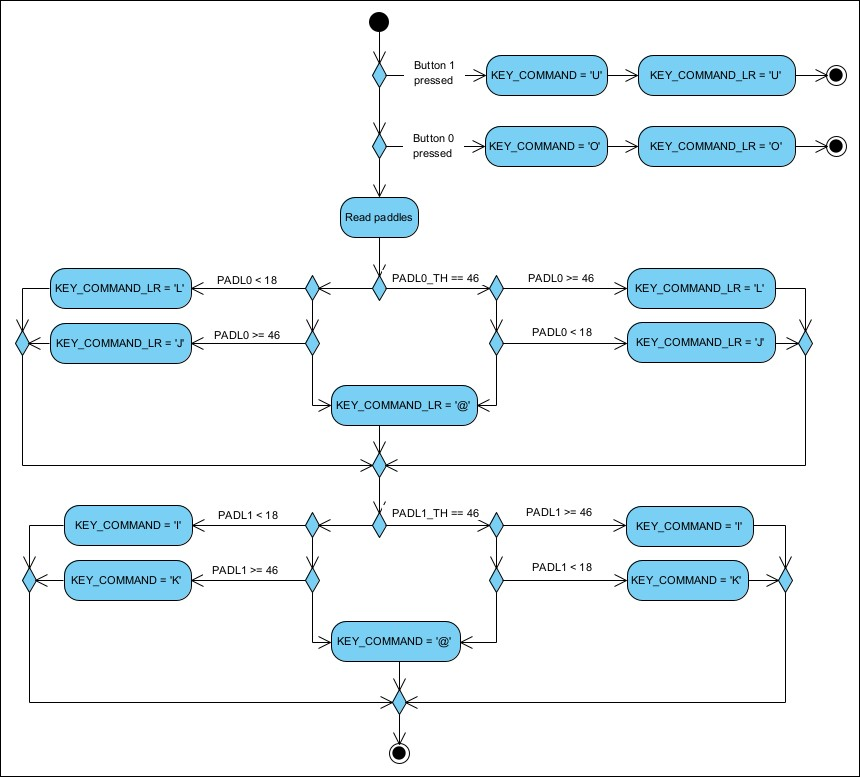
\includegraphics[width=\columnwidth]{read_joystick_for_command}
\end{center}


\nwenddocs{}\nwbegincode{422}\sublabel{NW1Xx3lK-1W8AJS-L}\nwmargintag{{\nwtagstyle{}\subpageref{NW1Xx3lK-1W8AJS-L}}}\moddef{tables~{\nwtagstyle{}\subpageref{NW1Xx3lK-1W8AJS-1}}}\plusendmoddef\nwstartdeflinemarkup\nwusesondefline{\\{NW1Xx3lK-1p0Y9w-1}}\nwprevnextdefs{NW1Xx3lK-1W8AJS-K}{NW1Xx3lK-1W8AJS-M}\nwenddeflinemarkup
    ORG     $6B81
\nwlinkedidentc{PADDLE0_THRESH1}{NW1Xx3lK-1W8AJS-L}:
    HEX     12
\nwlinkedidentc{PADDLE0_THRESH2}{NW1Xx3lK-1W8AJS-L}:
    HEX     2E
\nwlinkedidentc{PADDLE1_THRESH1}{NW1Xx3lK-1W8AJS-L}:
    HEX     12
\nwlinkedidentc{PADDLE1_THRESH2}{NW1Xx3lK-1W8AJS-L}:
    HEX     2E
\nwindexdefn{\nwixident{PADDLE0{\_}THRESH1}}{PADDLE0:unTHRESH1}{NW1Xx3lK-1W8AJS-L}\nwindexdefn{\nwixident{PADDLE0{\_}THRESH2}}{PADDLE0:unTHRESH2}{NW1Xx3lK-1W8AJS-L}\nwindexdefn{\nwixident{PADDLE1{\_}THRESH1}}{PADDLE1:unTHRESH1}{NW1Xx3lK-1W8AJS-L}\nwindexdefn{\nwixident{PADDLE1{\_}THRESH2}}{PADDLE1:unTHRESH2}{NW1Xx3lK-1W8AJS-L}\eatline
\nwused{\\{NW1Xx3lK-1p0Y9w-1}}\nwidentdefs{\\{{\nwixident{PADDLE0{\_}THRESH1}}{PADDLE0:unTHRESH1}}\\{{\nwixident{PADDLE0{\_}THRESH2}}{PADDLE0:unTHRESH2}}\\{{\nwixident{PADDLE1{\_}THRESH1}}{PADDLE1:unTHRESH1}}\\{{\nwixident{PADDLE1{\_}THRESH2}}{PADDLE1:unTHRESH2}}}\nwendcode{}\nwbegindocs{423}\nwdocspar
\nwenddocs{}\nwbegincode{424}\sublabel{NW1Xx3lK-3WwA9w-1}\nwmargintag{{\nwtagstyle{}\subpageref{NW1Xx3lK-3WwA9w-1}}}\moddef{check buttons~{\nwtagstyle{}\subpageref{NW1Xx3lK-3WwA9w-1}}}\endmoddef\nwstartdeflinemarkup\nwusesondefline{\\{NW1Xx3lK-8jv1b-C}}\nwenddeflinemarkup
    ORG     $6AD0
\nwlinkedidentc{READ_JOYSTICK_FOR_COMMAND}{NW1Xx3lK-3WwA9w-1}:
    SUBROUTINE

    LDA     \nwlinkedidentc{BUTN1}{NW1Xx3lK-10jlgu-I}
    BPL     .check_butn0
    LDA     #$D5                  ; 'U' (dig)
    BNE     .store_key_command    ; unconditional

.check_butn0:
    LDA     \nwlinkedidentc{BUTN0}{NW1Xx3lK-10jlgu-I}
    BPL     .read_paddles
    LDA     #$CF                  ; 'O' (dig)

.store_key_command
    STA     \nwlinkedidentc{KEY_COMMAND}{NW1Xx3lK-10jlgu-a}
    STA     \nwlinkedidentc{KEY_COMMAND_LR}{NW1Xx3lK-10jlgu-a}
    RTS

.read_paddles:
    JSR     \nwlinkedidentc{READ_PADDLES}{NW1Xx3lK-4UbpAF-1}
    LDY     \nwlinkedidentc{PADDLE0_VALUE}{NW1Xx3lK-10jlgu-H}

    LDA     \nwlinkedidentc{PADDLE0_THRESH2}{NW1Xx3lK-1W8AJS-L}
    CMP     #$2E
    BEQ     .6afa
    ; \nwlinkedidentc{PADDLE0_THRESH2}{NW1Xx3lK-1W8AJS-L} != 46

    CPY     \nwlinkedidentc{PADDLE0_THRESH2}{NW1Xx3lK-1W8AJS-L}
    BCS     .6b03
    ; \nwlinkedidentc{PADDLE0_VALUE}{NW1Xx3lK-10jlgu-H} < \nwlinkedidentc{PADDLE0_THRESH2}{NW1Xx3lK-1W8AJS-L}

    LDA     #$CC                  ; 'L' (right)
    BNE     .check_paddle_1       ; unconditional

.6afa:
    CPY     \nwlinkedidentc{PADDLE0_THRESH2}{NW1Xx3lK-1W8AJS-L}
    BCC     .6b03
    ; \nwlinkedidentc{PADDLE0_VALUE}{NW1Xx3lK-10jlgu-H} >= \nwlinkedidentc{PADDLE0_THRESH2}{NW1Xx3lK-1W8AJS-L}

    LDA     #$CC                  ; 'L' (right)
    BNE     .check_paddle_1       ; unconditional

.6b03:
    LDA     \nwlinkedidentc{PADDLE0_THRESH1}{NW1Xx3lK-1W8AJS-L}
    CMP     #$2E
    BEQ     .6b13
    ; \nwlinkedidentc{PADDLE0_THRESH1}{NW1Xx3lK-1W8AJS-L} != 46

    CPY     \nwlinkedidentc{PADDLE0_THRESH1}{NW1Xx3lK-1W8AJS-L}
    BCS     .6b1c
    ; \nwlinkedidentc{PADDLE0_VALUE}{NW1Xx3lK-10jlgu-H} < \nwlinkedidentc{PADDLE0_THRESH1}{NW1Xx3lK-1W8AJS-L}
    LDA     #$CA                  ; 'J' (left)
    BNE     .check_paddle_1       ; unconditional

.6b13:
    CPY     \nwlinkedidentc{PADDLE0_THRESH1}{NW1Xx3lK-1W8AJS-L}
    BCC     .6b1c
    ; \nwlinkedidentc{PADDLE0_VALUE}{NW1Xx3lK-10jlgu-H} >= \nwlinkedidentc{PADDLE0_THRESH1}{NW1Xx3lK-1W8AJS-L}
    LDA     #$CA                  ; 'J' (left)
    BNE     .check_paddle_1       ; unconditional

.6b1c:
    LDA     #$C0                   ; '@'

.check_paddle_1:
    STA     \nwlinkedidentc{KEY_COMMAND_LR}{NW1Xx3lK-10jlgu-a}

    LDY     \nwlinkedidentc{PADDLE1_VALUE}{NW1Xx3lK-10jlgu-H}

    LDA     \nwlinkedidentc{PADDLE1_THRESH1}{NW1Xx3lK-1W8AJS-L}
    CMP     #$2E
    BEQ     .6b32
    ; \nwlinkedidentc{PADDLE1_THRESH1}{NW1Xx3lK-1W8AJS-L} != 46

    CPY     \nwlinkedidentc{PADDLE1_THRESH1}{NW1Xx3lK-1W8AJS-L}
    BCS     .6b3b
    ; \nwlinkedidentc{PADDLE1_VALUE}{NW1Xx3lK-10jlgu-H} >= \nwlinkedidentc{PADDLE1_THRESH1}{NW1Xx3lK-1W8AJS-L}

    LDA     #$C9                         ; 'I' (up)
    BNE     .store_key_command_end       ; unconditional

.6b32:
    CPY     \nwlinkedidentc{PADDLE1_THRESH1}{NW1Xx3lK-1W8AJS-L}
    BCC     .6b3b
    ; \nwlinkedidentc{PADDLE1_VALUE}{NW1Xx3lK-10jlgu-H} < \nwlinkedidentc{PADDLE1_THRESH1}{NW1Xx3lK-1W8AJS-L}

    LDA     #$C9                         ; 'I' (up)
    BNE     .store_key_command_end       ; unconditional

.6b3b:
    LDA     \nwlinkedidentc{PADDLE1_THRESH2}{NW1Xx3lK-1W8AJS-L}
    CMP     #$2E
    BEQ     .6b4b
    ; \nwlinkedidentc{PADDLE1_THRESH2}{NW1Xx3lK-1W8AJS-L} != 46

    CPY     \nwlinkedidentc{PADDLE1_THRESH2}{NW1Xx3lK-1W8AJS-L}
    BCS     .6b54
    ; \nwlinkedidentc{PADDLE1_VALUE}{NW1Xx3lK-10jlgu-H} >= \nwlinkedidentc{PADDLE1_THRESH2}{NW1Xx3lK-1W8AJS-L}

    LDA     #$CB                         ; 'K' (down)
    BNE     .store_key_command_end       ; unconditional

.6b4b:
    CPY     \nwlinkedidentc{PADDLE1_THRESH2}{NW1Xx3lK-1W8AJS-L}
    BCC     .6b54
    ; \nwlinkedidentc{PADDLE1_VALUE}{NW1Xx3lK-10jlgu-H} < \nwlinkedidentc{PADDLE1_THRESH2}{NW1Xx3lK-1W8AJS-L}

    LDA     #$CB                         ; 'K' (down)
    BNE     .store_key_command_end       ; unconditional

.6b54:
    LDA     #$C0                         ; '@'

.store_key_command_end:
    STA     \nwlinkedidentc{KEY_COMMAND}{NW1Xx3lK-10jlgu-a}
    RTS

\nwindexdefn{\nwixident{READ{\_}JOYSTICK{\_}FOR{\_}COMMAND}}{READ:unJOYSTICK:unFOR:unCOMMAND}{NW1Xx3lK-3WwA9w-1}\eatline
\nwused{\\{NW1Xx3lK-8jv1b-C}}\nwidentdefs{\\{{\nwixident{READ{\_}JOYSTICK{\_}FOR{\_}COMMAND}}{READ:unJOYSTICK:unFOR:unCOMMAND}}}\nwidentuses{\\{{\nwixident{BUTN0}}{BUTN0}}\\{{\nwixident{BUTN1}}{BUTN1}}\\{{\nwixident{KEY{\_}COMMAND}}{KEY:unCOMMAND}}\\{{\nwixident{KEY{\_}COMMAND{\_}LR}}{KEY:unCOMMAND:unLR}}\\{{\nwixident{PADDLE0{\_}THRESH1}}{PADDLE0:unTHRESH1}}\\{{\nwixident{PADDLE0{\_}THRESH2}}{PADDLE0:unTHRESH2}}\\{{\nwixident{PADDLE0{\_}VALUE}}{PADDLE0:unVALUE}}\\{{\nwixident{PADDLE1{\_}THRESH1}}{PADDLE1:unTHRESH1}}\\{{\nwixident{PADDLE1{\_}THRESH2}}{PADDLE1:unTHRESH2}}\\{{\nwixident{PADDLE1{\_}VALUE}}{PADDLE1:unVALUE}}\\{{\nwixident{READ{\_}PADDLES}}{READ:unPADDLES}}}\nwindexuse{\nwixident{BUTN0}}{BUTN0}{NW1Xx3lK-3WwA9w-1}\nwindexuse{\nwixident{BUTN1}}{BUTN1}{NW1Xx3lK-3WwA9w-1}\nwindexuse{\nwixident{KEY{\_}COMMAND}}{KEY:unCOMMAND}{NW1Xx3lK-3WwA9w-1}\nwindexuse{\nwixident{KEY{\_}COMMAND{\_}LR}}{KEY:unCOMMAND:unLR}{NW1Xx3lK-3WwA9w-1}\nwindexuse{\nwixident{PADDLE0{\_}THRESH1}}{PADDLE0:unTHRESH1}{NW1Xx3lK-3WwA9w-1}\nwindexuse{\nwixident{PADDLE0{\_}THRESH2}}{PADDLE0:unTHRESH2}{NW1Xx3lK-3WwA9w-1}\nwindexuse{\nwixident{PADDLE0{\_}VALUE}}{PADDLE0:unVALUE}{NW1Xx3lK-3WwA9w-1}\nwindexuse{\nwixident{PADDLE1{\_}THRESH1}}{PADDLE1:unTHRESH1}{NW1Xx3lK-3WwA9w-1}\nwindexuse{\nwixident{PADDLE1{\_}THRESH2}}{PADDLE1:unTHRESH2}{NW1Xx3lK-3WwA9w-1}\nwindexuse{\nwixident{PADDLE1{\_}VALUE}}{PADDLE1:unVALUE}{NW1Xx3lK-3WwA9w-1}\nwindexuse{\nwixident{READ{\_}PADDLES}}{READ:unPADDLES}{NW1Xx3lK-3WwA9w-1}\nwendcode{}\nwbegindocs{425}\nwdocspar
\section{Player movement}

Player movement is generally handled by functions which check whether the player can
move in a given direction, and then either fail with carry set, or succeed, and the
player is moved, with carry cleared.

Recall that the player is at
the gross sprite location given by {\Tt{}\nwlinkedidentq{PLAYER{\_}COL}{NW1Xx3lK-10jlgu-M}\nwendquote} and {\Tt{}\nwlinkedidentq{PLAYER{\_}ROW}{NW1Xx3lK-10jlgu-M}\nwendquote}, but with a plus-or-minus
adjustment given by a horizontal adjustment {\Tt{}\nwlinkedidentq{PLAYER{\_}X{\_}ADJ}{NW1Xx3lK-10jlgu-P}\nwendquote} and a vertical adjustment {\Tt{}\nwlinkedidentq{PLAYER{\_}Y{\_}ADJ}{NW1Xx3lK-10jlgu-P}\nwendquote}.

We will refer to the player as
"exactly on" the sprite if the adjustment in the direction we're interested in is zero.
Again, recall that the adjustment values are offset by {\Tt{}2\nwendquote}, so an adjustment of zero is a value
of {\Tt{}2\nwendquote}, and the adjustment ranges from {\Tt{}-2\nwendquote} to {\Tt{}+2\nwendquote}.

We can refer to the player as slightly above, below, left of, or right of, an exact
sprite coordinate if the adjustment is not zero.

There are two routines which nudge the player towards an exact sprite row or column. Generally this
is done when the player does something that has to take place on an exact row or column, such as
climbing a ladder or traversing a rope, and serves to make the transition to an aligned row or column
more smooth. Each time the player is nudged, we also check if the player landed on gold.

\nwenddocs{}\nwbegincode{426}\sublabel{NW1Xx3lK-PXGvu-1}\nwmargintag{{\nwtagstyle{}\subpageref{NW1Xx3lK-PXGvu-1}}}\moddef{try moving up~{\nwtagstyle{}\subpageref{NW1Xx3lK-PXGvu-1}}}\endmoddef\nwstartdeflinemarkup\nwusesondefline{\\{NW1Xx3lK-8jv1b-C}}\nwprevnextdefs{\relax}{NW1Xx3lK-PXGvu-2}\nwenddeflinemarkup
    ORG     $6C13
\nwlinkedidentc{NUDGE_PLAYER_TOWARDS_EXACT_COLUMN}{NW1Xx3lK-PXGvu-1}:
    SUBROUTINE

    LDA     \nwlinkedidentc{PLAYER_X_ADJ}{NW1Xx3lK-10jlgu-P}
    CMP     #$02
    BCC     .player_slightly_left
    BEQ     .end

.player_slightly_right:
    DEC     \nwlinkedidentc{PLAYER_X_ADJ}{NW1Xx3lK-10jlgu-P}        ; Nudge player left
    JMP     \nwlinkedidentc{CHECK_FOR_GOLD_PICKED_UP_BY_PLAYER}{NW1Xx3lK-2zzVjv-1}

.player_slightly_left:
    INC     \nwlinkedidentc{PLAYER_X_ADJ}{NW1Xx3lK-10jlgu-P}        ; Nudge player right
    JMP     \nwlinkedidentc{CHECK_FOR_GOLD_PICKED_UP_BY_PLAYER}{NW1Xx3lK-2zzVjv-1}

.end:
    RTS

    ORG     $6C26
\nwlinkedidentc{NUDGE_PLAYER_TOWARDS_EXACT_ROW}{NW1Xx3lK-PXGvu-1}:
    SUBROUTINE

    LDA     \nwlinkedidentc{PLAYER_Y_ADJ}{NW1Xx3lK-10jlgu-P}
    CMP     #$02
    BCC     .player_slightly_above
    BEQ     .end

.player_slightly_below:
    DEC     \nwlinkedidentc{PLAYER_Y_ADJ}{NW1Xx3lK-10jlgu-P}        ; Nudge player up
    JMP     \nwlinkedidentc{CHECK_FOR_GOLD_PICKED_UP_BY_PLAYER}{NW1Xx3lK-2zzVjv-1}

.player_slightly_above:
    INC     \nwlinkedidentc{PLAYER_Y_ADJ}{NW1Xx3lK-10jlgu-P}        ; Nudge player down
    JMP     \nwlinkedidentc{CHECK_FOR_GOLD_PICKED_UP_BY_PLAYER}{NW1Xx3lK-2zzVjv-1}

.end:
    RTS

\nwindexdefn{\nwixident{NUDGE{\_}PLAYER{\_}TOWARDS{\_}EXACT{\_}COLUMN}}{NUDGE:unPLAYER:unTOWARDS:unEXACT:unCOLUMN}{NW1Xx3lK-PXGvu-1}\nwindexdefn{\nwixident{NUDGE{\_}PLAYER{\_}TOWARDS{\_}EXACT{\_}ROW}}{NUDGE:unPLAYER:unTOWARDS:unEXACT:unROW}{NW1Xx3lK-PXGvu-1}\eatline
\nwalsodefined{\\{NW1Xx3lK-PXGvu-2}}\nwused{\\{NW1Xx3lK-8jv1b-C}}\nwidentdefs{\\{{\nwixident{NUDGE{\_}PLAYER{\_}TOWARDS{\_}EXACT{\_}COLUMN}}{NUDGE:unPLAYER:unTOWARDS:unEXACT:unCOLUMN}}\\{{\nwixident{NUDGE{\_}PLAYER{\_}TOWARDS{\_}EXACT{\_}ROW}}{NUDGE:unPLAYER:unTOWARDS:unEXACT:unROW}}}\nwidentuses{\\{{\nwixident{CHECK{\_}FOR{\_}GOLD{\_}PICKED{\_}UP{\_}BY{\_}PLAYER}}{CHECK:unFOR:unGOLD:unPICKED:unUP:unBY:unPLAYER}}\\{{\nwixident{PLAYER{\_}X{\_}ADJ}}{PLAYER:unX:unADJ}}\\{{\nwixident{PLAYER{\_}Y{\_}ADJ}}{PLAYER:unY:unADJ}}}\nwindexuse{\nwixident{CHECK{\_}FOR{\_}GOLD{\_}PICKED{\_}UP{\_}BY{\_}PLAYER}}{CHECK:unFOR:unGOLD:unPICKED:unUP:unBY:unPLAYER}{NW1Xx3lK-PXGvu-1}\nwindexuse{\nwixident{PLAYER{\_}X{\_}ADJ}}{PLAYER:unX:unADJ}{NW1Xx3lK-PXGvu-1}\nwindexuse{\nwixident{PLAYER{\_}Y{\_}ADJ}}{PLAYER:unY:unADJ}{NW1Xx3lK-PXGvu-1}\nwendcode{}\nwbegindocs{427}\nwdocspar
Now the logic for attempting to move up is:

\begin{itemize}
  \item If the player location contains a ladder:
  \begin{itemize}
    \item If the player is slightly below the sprite, then move the player up.
    \item Otherwise, if the player is on row zero, the player cannot move up.
    \item Otherwise, if the sprite on the row above is brick, stone, or trap,
          the player cannot move up.
    \item Otherwise, the player can move up.
  \end{itemize}
  \item Otherwise:
  \begin{itemize}
    \item If the player is not slightly below the sprite, the player cannot move up.
    \item Otherwise, if the sprite on the row below is not a ladder, the player cannot move up.
    \item Otherwise, the player can move up.
  \end{itemize}
\end{itemize}

The steps involved in actually moving the player up are:

\begin{itemize}
    \item Erase the player sprite.
    \item Reduce any horizontal adjustment, checking for gold pickup if not already exactly on a sprite column.
    \item Adjust the player vertically upwards by decrementing {\Tt{}\nwlinkedidentq{PLAYER{\_}Y{\_}ADJ}{NW1Xx3lK-10jlgu-P}\nwendquote}.
    \item If the adjustment didn't roll over, check for gold pickup, then update
          the player animation for climbing, and draw the player.
    \item Otherwise:
    \begin{itemize}
        \item Copy the background sprite at the player's sprite location to the active page, unless
              that sprite is a brick, in which case place an empty on the active page.
        \item Decrement {\Tt{}\nwlinkedidentq{PLAYER{\_}ROW}{NW1Xx3lK-10jlgu-M}\nwendquote}.
        \item Put the player sprite on the active page at the new location.
        \item Set the player's vertical adjustment to {\Tt{}+2\nwendquote}.
        \item Update the player animation for climbing, and draw the player.
    \end{itemize}
\end{itemize}

\nwenddocs{}\nwbegincode{428}\sublabel{NW1Xx3lK-PXGvu-2}\nwmargintag{{\nwtagstyle{}\subpageref{NW1Xx3lK-PXGvu-2}}}\moddef{try moving up~{\nwtagstyle{}\subpageref{NW1Xx3lK-PXGvu-1}}}\plusendmoddef\nwstartdeflinemarkup\nwusesondefline{\\{NW1Xx3lK-8jv1b-C}}\nwprevnextdefs{NW1Xx3lK-PXGvu-1}{\relax}\nwenddeflinemarkup
    ORG     $66BD
\nwlinkedidentc{TRY_MOVING_UP}{NW1Xx3lK-PXGvu-2}:
    SUBROUTINE

    \LA{}get background sprite at player location~{\nwtagstyle{}\subpageref{NW1Xx3lK-1YOcYz-1}}\RA{}
    CMP     #SPRITE_LADDER
    BEQ     .ladder_here

    LDY     \nwlinkedidentc{PLAYER_Y_ADJ}{NW1Xx3lK-10jlgu-P}
    CPY     #$03
    BCC     .cannot_move       ; if \nwlinkedidentc{PLAYER_Y_ADJ}{NW1Xx3lK-10jlgu-P} <= 2

    ; and if there's no ladder below, you can't move up.
    \LA{}get background sprite at player location on next row~{\nwtagstyle{}\subpageref{NW1Xx3lK-1sZsTB-1}}\RA{}
    CMP     #SPRITE_LADDER
    BEQ     .move_player_up

.cannot_move:
    SEC
    RTS

.ladder_here:
    LDY     \nwlinkedidentc{PLAYER_Y_ADJ}{NW1Xx3lK-10jlgu-P}
    CPY     #$03
    BCS     .move_player_up             ; if \nwlinkedidentc{PLAYER_Y_ADJ}{NW1Xx3lK-10jlgu-P} > 2

    ; If you're at the top, you can't move up even if there's a ladder.
    LDY     \nwlinkedidentc{PLAYER_ROW}{NW1Xx3lK-10jlgu-M}
    BEQ     .cannot_move       ; if \nwlinkedidentc{PLAYER_ROW}{NW1Xx3lK-10jlgu-M} == 0, set carry and return

    ; You can't move up if there's a brick, stone, or trap above.
    LDA     \nwlinkedidentc{CURR_LEVEL_ROW_SPRITES_PTR_OFFSETS}{NW1Xx3lK-1W8AJS-C}-1,Y
    STA     \nwlinkedidentc{PTR1}{NW1Xx3lK-10jlgu-L}
    LDA     \nwlinkedidentc{CURR_LEVEL_ROW_SPRITES_PTR_PAGES}{NW1Xx3lK-1W8AJS-C}-1,Y
    STA     \nwlinkedidentc{PTR1}{NW1Xx3lK-10jlgu-L}+1
    LDY     \nwlinkedidentc{PLAYER_COL}{NW1Xx3lK-10jlgu-M}
    LDA     (\nwlinkedidentc{PTR1}{NW1Xx3lK-10jlgu-L}),Y                    ; Get the sprite on the row above.

    CMP     #SPRITE_BRICK
    BEQ     .cannot_move
    CMP     #SPRITE_STONE
    BEQ     .cannot_move
    CMP     #SPRITE_TRAP
    BEQ     .cannot_move       ; If brick, stone, or trap, set carry and return

.move_player_up:
    JSR     \nwlinkedidentc{GET_SPRITE_AND_SCREEN_COORD_AT_PLAYER}{NW1Xx3lK-24XK8J-1}
    JSR     \nwlinkedidentc{ERASE_SPRITE_AT_PIXEL_COORDS}{NW1Xx3lK-xFyle-1}
    LDY     \nwlinkedidentc{PLAYER_ROW}{NW1Xx3lK-10jlgu-M}
    \LA{}set active and background row pointers \code{}PTR1\edoc{} and \code{}PTR2\edoc{} for \code{}Y\edoc{}~{\nwtagstyle{}\subpageref{NW1Xx3lK-4cENZH-1}}\RA{}
    JSR     \nwlinkedidentc{NUDGE_PLAYER_TOWARDS_EXACT_COLUMN}{NW1Xx3lK-PXGvu-1}
    DEC     \nwlinkedidentc{PLAYER_Y_ADJ}{NW1Xx3lK-10jlgu-P}                ; Move player up
    BPL     TRY_MOVING_UP_check_for_gold

    ; \nwlinkedidentc{PLAYER_Y_ADJ}{NW1Xx3lK-10jlgu-P} rolled over.

    ; Restore the sprite at the player's former location:
    ; If background page at player location is brick, put an empty at the
    ; (previous) player location on active page, otherwise copy the background
    ; sprite to the active page.
    LDY     \nwlinkedidentc{PLAYER_COL}{NW1Xx3lK-10jlgu-M}
    LDA     (\nwlinkedidentc{PTR2}{NW1Xx3lK-10jlgu-L}),Y
    CMP     #SPRITE_BRICK
    BNE     .set_on_real_page
    LDA     #SPRITE_EMPTY
.set_on_real_page:
    STA     (\nwlinkedidentc{PTR1}{NW1Xx3lK-10jlgu-L}),Y

    DEC     \nwlinkedidentc{PLAYER_ROW}{NW1Xx3lK-10jlgu-M}                  ; Move player up
    LDY     \nwlinkedidentc{PLAYER_ROW}{NW1Xx3lK-10jlgu-M}
    \LA{}set active row pointer \code{}PTR1\edoc{} for \code{}Y\edoc{}~{\nwtagstyle{}\subpageref{NW1Xx3lK-qxK9U-1}}\RA{}
    LDY     \nwlinkedidentc{PLAYER_COL}{NW1Xx3lK-10jlgu-M}
    LDA     #SPRITE_PLAYER
    STA     (\nwlinkedidentc{PTR1}{NW1Xx3lK-10jlgu-L}),Y            ; Write player sprite to active page.
    LDA     #$04
    STA     \nwlinkedidentc{PLAYER_Y_ADJ}{NW1Xx3lK-10jlgu-P}        ; Set adjustment to +2
    BNE     TRY_MOVING_UP_inc_anim_state     ; unconditional

TRY_MOVING_UP_check_for_gold:
    JSR     \nwlinkedidentc{CHECK_FOR_GOLD_PICKED_UP_BY_PLAYER}{NW1Xx3lK-2zzVjv-1}

TRY_MOVING_UP_inc_anim_state:
    LDA     #$10
    LDX     #$11
    JSR     \nwlinkedidentc{INC_ANIM_STATE}{NW1Xx3lK-21IDEw-1}      ; player climbing on ladder
    JSR     \nwlinkedidentc{DRAW_PLAYER}{NW1Xx3lK-2x2oAB-1}
    CLC
    RTS
\nwindexdefn{\nwixident{TRY{\_}MOVING{\_}UP}}{TRY:unMOVING:unUP}{NW1Xx3lK-PXGvu-2}\eatline
\nwused{\\{NW1Xx3lK-8jv1b-C}}\nwidentdefs{\\{{\nwixident{TRY{\_}MOVING{\_}UP}}{TRY:unMOVING:unUP}}}\nwidentuses{\\{{\nwixident{CHECK{\_}FOR{\_}GOLD{\_}PICKED{\_}UP{\_}BY{\_}PLAYER}}{CHECK:unFOR:unGOLD:unPICKED:unUP:unBY:unPLAYER}}\\{{\nwixident{CURR{\_}LEVEL{\_}ROW{\_}SPRITES{\_}PTR{\_}OFFSETS}}{CURR:unLEVEL:unROW:unSPRITES:unPTR:unOFFSETS}}\\{{\nwixident{CURR{\_}LEVEL{\_}ROW{\_}SPRITES{\_}PTR{\_}PAGES}}{CURR:unLEVEL:unROW:unSPRITES:unPTR:unPAGES}}\\{{\nwixident{DRAW{\_}PLAYER}}{DRAW:unPLAYER}}\\{{\nwixident{ERASE{\_}SPRITE{\_}AT{\_}PIXEL{\_}COORDS}}{ERASE:unSPRITE:unAT:unPIXEL:unCOORDS}}\\{{\nwixident{GET{\_}SPRITE{\_}AND{\_}SCREEN{\_}COORD{\_}AT{\_}PLAYER}}{GET:unSPRITE:unAND:unSCREEN:unCOORD:unAT:unPLAYER}}\\{{\nwixident{INC{\_}ANIM{\_}STATE}}{INC:unANIM:unSTATE}}\\{{\nwixident{NUDGE{\_}PLAYER{\_}TOWARDS{\_}EXACT{\_}COLUMN}}{NUDGE:unPLAYER:unTOWARDS:unEXACT:unCOLUMN}}\\{{\nwixident{PLAYER{\_}COL}}{PLAYER:unCOL}}\\{{\nwixident{PLAYER{\_}ROW}}{PLAYER:unROW}}\\{{\nwixident{PLAYER{\_}Y{\_}ADJ}}{PLAYER:unY:unADJ}}\\{{\nwixident{PTR1}}{PTR1}}\\{{\nwixident{PTR2}}{PTR2}}}\nwindexuse{\nwixident{CHECK{\_}FOR{\_}GOLD{\_}PICKED{\_}UP{\_}BY{\_}PLAYER}}{CHECK:unFOR:unGOLD:unPICKED:unUP:unBY:unPLAYER}{NW1Xx3lK-PXGvu-2}\nwindexuse{\nwixident{CURR{\_}LEVEL{\_}ROW{\_}SPRITES{\_}PTR{\_}OFFSETS}}{CURR:unLEVEL:unROW:unSPRITES:unPTR:unOFFSETS}{NW1Xx3lK-PXGvu-2}\nwindexuse{\nwixident{CURR{\_}LEVEL{\_}ROW{\_}SPRITES{\_}PTR{\_}PAGES}}{CURR:unLEVEL:unROW:unSPRITES:unPTR:unPAGES}{NW1Xx3lK-PXGvu-2}\nwindexuse{\nwixident{DRAW{\_}PLAYER}}{DRAW:unPLAYER}{NW1Xx3lK-PXGvu-2}\nwindexuse{\nwixident{ERASE{\_}SPRITE{\_}AT{\_}PIXEL{\_}COORDS}}{ERASE:unSPRITE:unAT:unPIXEL:unCOORDS}{NW1Xx3lK-PXGvu-2}\nwindexuse{\nwixident{GET{\_}SPRITE{\_}AND{\_}SCREEN{\_}COORD{\_}AT{\_}PLAYER}}{GET:unSPRITE:unAND:unSCREEN:unCOORD:unAT:unPLAYER}{NW1Xx3lK-PXGvu-2}\nwindexuse{\nwixident{INC{\_}ANIM{\_}STATE}}{INC:unANIM:unSTATE}{NW1Xx3lK-PXGvu-2}\nwindexuse{\nwixident{NUDGE{\_}PLAYER{\_}TOWARDS{\_}EXACT{\_}COLUMN}}{NUDGE:unPLAYER:unTOWARDS:unEXACT:unCOLUMN}{NW1Xx3lK-PXGvu-2}\nwindexuse{\nwixident{PLAYER{\_}COL}}{PLAYER:unCOL}{NW1Xx3lK-PXGvu-2}\nwindexuse{\nwixident{PLAYER{\_}ROW}}{PLAYER:unROW}{NW1Xx3lK-PXGvu-2}\nwindexuse{\nwixident{PLAYER{\_}Y{\_}ADJ}}{PLAYER:unY:unADJ}{NW1Xx3lK-PXGvu-2}\nwindexuse{\nwixident{PTR1}}{PTR1}{NW1Xx3lK-PXGvu-2}\nwindexuse{\nwixident{PTR2}}{PTR2}{NW1Xx3lK-PXGvu-2}\nwendcode{}\nwbegindocs{429}\nwdocspar
For attempting to move down, the logic is:

\begin{itemize}
  \item If the player is slightly above the sprite, then move the player down.
  \item Otherwise, if the player is on row 15 or more, the player cannot move down.
  \item Otherwise, if the row below is stone or brick, the player cannot move down.
  \item Otherwise, the player can move down.
\end{itemize}

The steps involved in actually moving the player down are:

\begin{itemize}
    \item Erase the player sprite.
    \item Reduce any horizontal adjustment, checking for gold pickup if not already exactly on a sprite column.
    \item Adjust the player vertically downwards by incrementing {\Tt{}\nwlinkedidentq{PLAYER{\_}Y{\_}ADJ}{NW1Xx3lK-10jlgu-P}\nwendquote}.
    \item If the adjustment didn't roll over, check for gold pickup, then update
          the player animation for climbing, and draw the player.
    \item Otherwise:
    \begin{itemize}
        \item Copy the background sprite at the player's sprite location to the active page, unless
              that sprite is a brick, in which case place an empty on the active page.
        \item Increment {\Tt{}\nwlinkedidentq{PLAYER{\_}ROW}{NW1Xx3lK-10jlgu-M}\nwendquote}.
        \item Put the player sprite on the active page at the new location.
        \item Set the player's vertical adjustment to {\Tt{}-2\nwendquote}.
        \item Update the player animation for climbing, and draw the player.
    \end{itemize}
\end{itemize}

\nwenddocs{}\nwbegincode{430}\sublabel{NW1Xx3lK-3I7nQV-1}\nwmargintag{{\nwtagstyle{}\subpageref{NW1Xx3lK-3I7nQV-1}}}\moddef{try moving down~{\nwtagstyle{}\subpageref{NW1Xx3lK-3I7nQV-1}}}\endmoddef\nwstartdeflinemarkup\nwusesondefline{\\{NW1Xx3lK-8jv1b-C}}\nwenddeflinemarkup
    ORG     $6766
\nwlinkedidentc{TRY_MOVING_DOWN}{NW1Xx3lK-3I7nQV-1}:
    SUBROUTINE

    LDY     \nwlinkedidentc{PLAYER_Y_ADJ}{NW1Xx3lK-10jlgu-P}
    CPY     #$02
    BCC     .move_player_down   ; player slightly above, so can move down.

    LDY     \nwlinkedidentc{PLAYER_ROW}{NW1Xx3lK-10jlgu-M}
    CPY     #MAX_GAME_ROW
    BCS     .cannot_move        ; player on row >= 15, so cannot move.

    \LA{}set active row pointer \code{}PTR1\edoc{} for \code{}Y+1\edoc{}~{\nwtagstyle{}\subpageref{NW1Xx3lK-GJ9rI-1}}\RA{}
    LDY     \nwlinkedidentc{PLAYER_COL}{NW1Xx3lK-10jlgu-M}
    LDA     (\nwlinkedidentc{PTR1}{NW1Xx3lK-10jlgu-L}),Y
    CMP     #SPRITE_STONE
    BEQ     .cannot_move
    CMP     #SPRITE_BRICK
    BNE     .move_player_down   ; Row below is stone or brick, so cannot move.

.cannot_move:
    SEC
    RTS

.move_player_down:
    JSR     \nwlinkedidentc{GET_SPRITE_AND_SCREEN_COORD_AT_PLAYER}{NW1Xx3lK-24XK8J-1}
    JSR     \nwlinkedidentc{ERASE_SPRITE_AT_PIXEL_COORDS}{NW1Xx3lK-xFyle-1}
    LDY     \nwlinkedidentc{PLAYER_ROW}{NW1Xx3lK-10jlgu-M}
    \LA{}set active and background row pointers \code{}PTR1\edoc{} and \code{}PTR2\edoc{} for \code{}Y\edoc{}~{\nwtagstyle{}\subpageref{NW1Xx3lK-4cENZH-1}}\RA{}
    JSR     \nwlinkedidentc{NUDGE_PLAYER_TOWARDS_EXACT_COLUMN}{NW1Xx3lK-PXGvu-1}
    INC     \nwlinkedidentc{PLAYER_Y_ADJ}{NW1Xx3lK-10jlgu-P}                ; Move player down
    LDA     \nwlinkedidentc{PLAYER_Y_ADJ}{NW1Xx3lK-10jlgu-P}
    CMP     #$05
    BCC     .check_for_gold_

    ; adjustment overflow
    LDY     \nwlinkedidentc{PLAYER_COL}{NW1Xx3lK-10jlgu-M}
    LDA     (\nwlinkedidentc{PTR2}{NW1Xx3lK-10jlgu-L}),Y
    CMP     #SPRITE_BRICK
    BNE     .set_on_real_page
    LDA     #SPRITE_EMPTY
.set_on_real_page:
    STA     (\nwlinkedidentc{PTR1}{NW1Xx3lK-10jlgu-L}),Y

    INC     \nwlinkedidentc{PLAYER_ROW}{NW1Xx3lK-10jlgu-M}
    LDY     \nwlinkedidentc{PLAYER_ROW}{NW1Xx3lK-10jlgu-M}
    \LA{}set active row pointer \code{}PTR1\edoc{} for \code{}Y\edoc{}~{\nwtagstyle{}\subpageref{NW1Xx3lK-qxK9U-1}}\RA{}
    LDY     \nwlinkedidentc{PLAYER_COL}{NW1Xx3lK-10jlgu-M}
    LDA     #SPRITE_PLAYER
    STA     (\nwlinkedidentc{PTR1}{NW1Xx3lK-10jlgu-L}),Y            ; Write player sprite to active page.
    LDA     #SPRITE_EMPTY
    STA     \nwlinkedidentc{PLAYER_Y_ADJ}{NW1Xx3lK-10jlgu-P}        ; Set adjustment to -2
    JMP     TRY_MOVING_UP_inc_anim_state

.check_for_gold_:
    JMP     TRY_MOVING_UP_check_for_gold
\nwindexdefn{\nwixident{TRY{\_}MOVING{\_}DOWN}}{TRY:unMOVING:unDOWN}{NW1Xx3lK-3I7nQV-1}\eatline
\nwused{\\{NW1Xx3lK-8jv1b-C}}\nwidentdefs{\\{{\nwixident{TRY{\_}MOVING{\_}DOWN}}{TRY:unMOVING:unDOWN}}}\nwidentuses{\\{{\nwixident{ERASE{\_}SPRITE{\_}AT{\_}PIXEL{\_}COORDS}}{ERASE:unSPRITE:unAT:unPIXEL:unCOORDS}}\\{{\nwixident{GET{\_}SPRITE{\_}AND{\_}SCREEN{\_}COORD{\_}AT{\_}PLAYER}}{GET:unSPRITE:unAND:unSCREEN:unCOORD:unAT:unPLAYER}}\\{{\nwixident{NUDGE{\_}PLAYER{\_}TOWARDS{\_}EXACT{\_}COLUMN}}{NUDGE:unPLAYER:unTOWARDS:unEXACT:unCOLUMN}}\\{{\nwixident{PLAYER{\_}COL}}{PLAYER:unCOL}}\\{{\nwixident{PLAYER{\_}ROW}}{PLAYER:unROW}}\\{{\nwixident{PLAYER{\_}Y{\_}ADJ}}{PLAYER:unY:unADJ}}\\{{\nwixident{PTR1}}{PTR1}}\\{{\nwixident{PTR2}}{PTR2}}}\nwindexuse{\nwixident{ERASE{\_}SPRITE{\_}AT{\_}PIXEL{\_}COORDS}}{ERASE:unSPRITE:unAT:unPIXEL:unCOORDS}{NW1Xx3lK-3I7nQV-1}\nwindexuse{\nwixident{GET{\_}SPRITE{\_}AND{\_}SCREEN{\_}COORD{\_}AT{\_}PLAYER}}{GET:unSPRITE:unAND:unSCREEN:unCOORD:unAT:unPLAYER}{NW1Xx3lK-3I7nQV-1}\nwindexuse{\nwixident{NUDGE{\_}PLAYER{\_}TOWARDS{\_}EXACT{\_}COLUMN}}{NUDGE:unPLAYER:unTOWARDS:unEXACT:unCOLUMN}{NW1Xx3lK-3I7nQV-1}\nwindexuse{\nwixident{PLAYER{\_}COL}}{PLAYER:unCOL}{NW1Xx3lK-3I7nQV-1}\nwindexuse{\nwixident{PLAYER{\_}ROW}}{PLAYER:unROW}{NW1Xx3lK-3I7nQV-1}\nwindexuse{\nwixident{PLAYER{\_}Y{\_}ADJ}}{PLAYER:unY:unADJ}{NW1Xx3lK-3I7nQV-1}\nwindexuse{\nwixident{PTR1}}{PTR1}{NW1Xx3lK-3I7nQV-1}\nwindexuse{\nwixident{PTR2}}{PTR2}{NW1Xx3lK-3I7nQV-1}\nwendcode{}\nwbegindocs{431}\nwdocspar
For attempting to move left, the logic is:

\begin{itemize}
  \item If the player is slightly right of the sprite, then move the player left.
  \item Otherwise, if the player is on column 0, the player cannot move left.
  \item Otherwise, if the column to the left is stone, brick, or trap, the player cannot move left.
  \item Otherwise, the player can move left.
\end{itemize}

The steps involved in actually moving the player left are:

\begin{itemize}
    \item Erase the player sprite.
    \item Set the {\Tt{}PLAYER{\_}FACING{\_}DIRECTION\nwendquote} to left ({\Tt{}0xFF\nwendquote}).
    \item Reduce any vertical adjustment, checking for gold pickup if not already exactly on a sprite column.
    \item Adjust the player horizontally to the left by decrementing {\Tt{}\nwlinkedidentq{PLAYER{\_}X{\_}ADJ}{NW1Xx3lK-10jlgu-P}\nwendquote}.
    \item If the adjustment didn't roll over, check for gold pickup, then update
          the player animation for moving left, and draw the player.
    \item Otherwise:
    \begin{itemize}
        \item Copy the background sprite at the player's sprite location to the active page, unless
              that sprite is a brick, in which case place an empty on the active page.
        \item Decrement {\Tt{}\nwlinkedidentq{PLAYER{\_}COL}{NW1Xx3lK-10jlgu-M}\nwendquote}.
        \item Put the player sprite on the active page at the new location.
        \item Set the player's horizontal adjustment to {\Tt{}+2\nwendquote}.
        \item Update the player animation for moving left, and draw the player.
    \end{itemize}
\end{itemize}

The animation is either monkey-traversing if the player moves onto a rope, or running otherwise.

\nwenddocs{}\nwbegincode{432}\sublabel{NW1Xx3lK-443qw5-1}\nwmargintag{{\nwtagstyle{}\subpageref{NW1Xx3lK-443qw5-1}}}\moddef{try moving left~{\nwtagstyle{}\subpageref{NW1Xx3lK-443qw5-1}}}\endmoddef\nwstartdeflinemarkup\nwusesondefline{\\{NW1Xx3lK-8jv1b-C}}\nwenddeflinemarkup
    ORG     $65D3
\nwlinkedidentc{TRY_MOVING_LEFT}{NW1Xx3lK-443qw5-1}:
    SUBROUTINE

    LDY     \nwlinkedidentc{PLAYER_ROW}{NW1Xx3lK-10jlgu-M}
    \LA{}set active and background row pointers \code{}PTR1\edoc{} and \code{}PTR2\edoc{} for \code{}Y\edoc{}~{\nwtagstyle{}\subpageref{NW1Xx3lK-4cENZH-1}}\RA{}
    LDX     \nwlinkedidentc{PLAYER_X_ADJ}{NW1Xx3lK-10jlgu-P}
    CPX     #$03
    BCS     .move_player_left       ; player slightly right, so can move left.

    LDY     \nwlinkedidentc{PLAYER_COL}{NW1Xx3lK-10jlgu-M}  
    BEQ     .cannot_move            ; col == 0, so cannot move.

    DEY
    LDA     (\nwlinkedidentc{PTR1}{NW1Xx3lK-10jlgu-L}),Y
    CMP     #SPRITE_STONE
    BEQ     .cannot_move
    CMP     #SPRITE_BRICK
    BEQ     .cannot_move
    CMP     #SPRITE_TRAP
    BNE     .move_player_left       ; brick, stone, or trap to left, so cannot move.

.cannot_move:
    RTS

.move_player_left:
    JSR     \nwlinkedidentc{GET_SPRITE_AND_SCREEN_COORD_AT_PLAYER}{NW1Xx3lK-24XK8J-1}
    JSR     \nwlinkedidentc{ERASE_SPRITE_AT_PIXEL_COORDS}{NW1Xx3lK-xFyle-1}
    LDA     #$FF
    STA     PLAYER_FACING_DIRECTION             ; face left
    JSR     \nwlinkedidentc{NUDGE_PLAYER_TOWARDS_EXACT_ROW}{NW1Xx3lK-PXGvu-1}
    DEC     \nwlinkedidentc{PLAYER_X_ADJ}{NW1Xx3lK-10jlgu-P}
    BPL     .check_for_gold

    ; adjustment overflow
    LDY     \nwlinkedidentc{PLAYER_COL}{NW1Xx3lK-10jlgu-M}
    LDA     (\nwlinkedidentc{PTR2}{NW1Xx3lK-10jlgu-L}),Y
    CMP     #SPRITE_BRICK
    BNE     .set_on_level
    LDA     #SPRITE_EMPTY
.set_on_level:
    STA     (\nwlinkedidentc{PTR1}{NW1Xx3lK-10jlgu-L}),Y

    DEC     \nwlinkedidentc{PLAYER_COL}{NW1Xx3lK-10jlgu-M}
    DEY
    LDA     #SPRITE_PLAYER
    STA     (\nwlinkedidentc{PTR1}{NW1Xx3lK-10jlgu-L}),Y            ; Write player sprite to active page.
    LDA     #$04
    STA     \nwlinkedidentc{PLAYER_X_ADJ}{NW1Xx3lK-10jlgu-P}        ; Set adjustment to +2
    BNE     .inc_anim_state     ; Unconditional

.check_for_gold:
    JSR     \nwlinkedidentc{CHECK_FOR_GOLD_PICKED_UP_BY_PLAYER}{NW1Xx3lK-2zzVjv-1}

.inc_anim_state:
    LDY     \nwlinkedidentc{PLAYER_COL}{NW1Xx3lK-10jlgu-M}
    LDA     (\nwlinkedidentc{PTR2}{NW1Xx3lK-10jlgu-L}),Y
    CMP     #SPRITE_ROPE
    BEQ     .anim_state_monkeying

    LDA     #$00
    LDX     #$02
    BNE     .done               ; Unconditional

.anim_state_monkeying:
    LDA     #$03
    LDX     #$05

.done:
    JSR     \nwlinkedidentc{INC_ANIM_STATE}{NW1Xx3lK-21IDEw-1}
    JMP     \nwlinkedidentc{DRAW_PLAYER}{NW1Xx3lK-2x2oAB-1}
\nwindexdefn{\nwixident{TRY{\_}MOVING{\_}LEFT}}{TRY:unMOVING:unLEFT}{NW1Xx3lK-443qw5-1}\eatline
\nwused{\\{NW1Xx3lK-8jv1b-C}}\nwidentdefs{\\{{\nwixident{TRY{\_}MOVING{\_}LEFT}}{TRY:unMOVING:unLEFT}}}\nwidentuses{\\{{\nwixident{CHECK{\_}FOR{\_}GOLD{\_}PICKED{\_}UP{\_}BY{\_}PLAYER}}{CHECK:unFOR:unGOLD:unPICKED:unUP:unBY:unPLAYER}}\\{{\nwixident{DRAW{\_}PLAYER}}{DRAW:unPLAYER}}\\{{\nwixident{ERASE{\_}SPRITE{\_}AT{\_}PIXEL{\_}COORDS}}{ERASE:unSPRITE:unAT:unPIXEL:unCOORDS}}\\{{\nwixident{GET{\_}SPRITE{\_}AND{\_}SCREEN{\_}COORD{\_}AT{\_}PLAYER}}{GET:unSPRITE:unAND:unSCREEN:unCOORD:unAT:unPLAYER}}\\{{\nwixident{INC{\_}ANIM{\_}STATE}}{INC:unANIM:unSTATE}}\\{{\nwixident{NUDGE{\_}PLAYER{\_}TOWARDS{\_}EXACT{\_}ROW}}{NUDGE:unPLAYER:unTOWARDS:unEXACT:unROW}}\\{{\nwixident{PLAYER{\_}COL}}{PLAYER:unCOL}}\\{{\nwixident{PLAYER{\_}ROW}}{PLAYER:unROW}}\\{{\nwixident{PLAYER{\_}X{\_}ADJ}}{PLAYER:unX:unADJ}}\\{{\nwixident{PTR1}}{PTR1}}\\{{\nwixident{PTR2}}{PTR2}}}\nwindexuse{\nwixident{CHECK{\_}FOR{\_}GOLD{\_}PICKED{\_}UP{\_}BY{\_}PLAYER}}{CHECK:unFOR:unGOLD:unPICKED:unUP:unBY:unPLAYER}{NW1Xx3lK-443qw5-1}\nwindexuse{\nwixident{DRAW{\_}PLAYER}}{DRAW:unPLAYER}{NW1Xx3lK-443qw5-1}\nwindexuse{\nwixident{ERASE{\_}SPRITE{\_}AT{\_}PIXEL{\_}COORDS}}{ERASE:unSPRITE:unAT:unPIXEL:unCOORDS}{NW1Xx3lK-443qw5-1}\nwindexuse{\nwixident{GET{\_}SPRITE{\_}AND{\_}SCREEN{\_}COORD{\_}AT{\_}PLAYER}}{GET:unSPRITE:unAND:unSCREEN:unCOORD:unAT:unPLAYER}{NW1Xx3lK-443qw5-1}\nwindexuse{\nwixident{INC{\_}ANIM{\_}STATE}}{INC:unANIM:unSTATE}{NW1Xx3lK-443qw5-1}\nwindexuse{\nwixident{NUDGE{\_}PLAYER{\_}TOWARDS{\_}EXACT{\_}ROW}}{NUDGE:unPLAYER:unTOWARDS:unEXACT:unROW}{NW1Xx3lK-443qw5-1}\nwindexuse{\nwixident{PLAYER{\_}COL}}{PLAYER:unCOL}{NW1Xx3lK-443qw5-1}\nwindexuse{\nwixident{PLAYER{\_}ROW}}{PLAYER:unROW}{NW1Xx3lK-443qw5-1}\nwindexuse{\nwixident{PLAYER{\_}X{\_}ADJ}}{PLAYER:unX:unADJ}{NW1Xx3lK-443qw5-1}\nwindexuse{\nwixident{PTR1}}{PTR1}{NW1Xx3lK-443qw5-1}\nwindexuse{\nwixident{PTR2}}{PTR2}{NW1Xx3lK-443qw5-1}\nwendcode{}\nwbegindocs{433}\nwdocspar
Moving right has the same logic as moving left, except in the other direction.

\nwenddocs{}\nwbegincode{434}\sublabel{NW1Xx3lK-2fpnEm-1}\nwmargintag{{\nwtagstyle{}\subpageref{NW1Xx3lK-2fpnEm-1}}}\moddef{try moving right~{\nwtagstyle{}\subpageref{NW1Xx3lK-2fpnEm-1}}}\endmoddef\nwstartdeflinemarkup\nwusesondefline{\\{NW1Xx3lK-8jv1b-C}}\nwenddeflinemarkup
    ORG     $6645
\nwlinkedidentc{TRY_MOVING_RIGHT}{NW1Xx3lK-2fpnEm-1}:
    SUBROUTINE

    LDY     \nwlinkedidentc{PLAYER_ROW}{NW1Xx3lK-10jlgu-M}
    \LA{}set active and background row pointers \code{}PTR1\edoc{} and \code{}PTR2\edoc{} for \code{}Y\edoc{}~{\nwtagstyle{}\subpageref{NW1Xx3lK-4cENZH-1}}\RA{}
    LDX     \nwlinkedidentc{PLAYER_X_ADJ}{NW1Xx3lK-10jlgu-P}
    CPX     #$02
    BCC     .move_player_right      ; player slightly left, so can move right.

    LDY     \nwlinkedidentc{PLAYER_COL}{NW1Xx3lK-10jlgu-M}
    CPY     #MAX_GAME_COL
    BEQ     .cannot_move            ; col == 27, so cannot move.

    INY
    LDA     (\nwlinkedidentc{PTR1}{NW1Xx3lK-10jlgu-L}),Y
    CMP     #SPRITE_STONE
    BEQ     .cannot_move
    CMP     #SPRITE_BRICK
    BEQ     .cannot_move
    CMP     #SPRITE_TRAP
    BNE     .move_player_right      ; brick, stone, or trap to right, so cannot move.

.cannot_move:
    RTS

.move_player_right:
    JSR     \nwlinkedidentc{GET_SPRITE_AND_SCREEN_COORD_AT_PLAYER}{NW1Xx3lK-24XK8J-1}
    JSR     \nwlinkedidentc{ERASE_SPRITE_AT_PIXEL_COORDS}{NW1Xx3lK-xFyle-1}
    LDA     #$01
    STA     PLAYER_FACING_DIRECTION             ; face right
    JSR     \nwlinkedidentc{NUDGE_PLAYER_TOWARDS_EXACT_ROW}{NW1Xx3lK-PXGvu-1}
    INC     \nwlinkedidentc{PLAYER_X_ADJ}{NW1Xx3lK-10jlgu-P}
    LDA     \nwlinkedidentc{PLAYER_X_ADJ}{NW1Xx3lK-10jlgu-P}
    CMP     #$05
    BCC     .check_for_gold

    ; adjustment overflow
    LDY     \nwlinkedidentc{PLAYER_COL}{NW1Xx3lK-10jlgu-M}
    LDA     (\nwlinkedidentc{PTR2}{NW1Xx3lK-10jlgu-L}),Y
    CMP     #SPRITE_BRICK
    BNE     .set_on_level
    LDA     #SPRITE_EMPTY
.set_on_level:
    STA     (\nwlinkedidentc{PTR1}{NW1Xx3lK-10jlgu-L}),Y

    INC     \nwlinkedidentc{PLAYER_COL}{NW1Xx3lK-10jlgu-M}
    INY
    LDA     #SPRITE_PLAYER
    STA     (\nwlinkedidentc{PTR1}{NW1Xx3lK-10jlgu-L}),Y            ; Write player sprite to active page.
    LDA     #$00
    STA     \nwlinkedidentc{PLAYER_X_ADJ}{NW1Xx3lK-10jlgu-P}        ; Set adjustment to -2
    BEQ     .inc_anim_state     ; Unconditional

.check_for_gold:
    JSR     \nwlinkedidentc{CHECK_FOR_GOLD_PICKED_UP_BY_PLAYER}{NW1Xx3lK-2zzVjv-1}

.inc_anim_state:
    LDY     \nwlinkedidentc{PLAYER_COL}{NW1Xx3lK-10jlgu-M}
    LDA     (\nwlinkedidentc{PTR2}{NW1Xx3lK-10jlgu-L}),Y
    CMP     #SPRITE_ROPE
    BEQ     .anim_state_monkeying

    LDA     #$08
    LDX     #$0A
    BNE     .done               ; Unconditional

.anim_state_monkeying:
    LDA     #$0B
    LDX     #$0D

.done:
    JSR     \nwlinkedidentc{INC_ANIM_STATE}{NW1Xx3lK-21IDEw-1}
    JMP     \nwlinkedidentc{DRAW_PLAYER}{NW1Xx3lK-2x2oAB-1}
\nwindexdefn{\nwixident{TRY{\_}MOVING{\_}RIGHT}}{TRY:unMOVING:unRIGHT}{NW1Xx3lK-2fpnEm-1}\eatline
\nwused{\\{NW1Xx3lK-8jv1b-C}}\nwidentdefs{\\{{\nwixident{TRY{\_}MOVING{\_}RIGHT}}{TRY:unMOVING:unRIGHT}}}\nwidentuses{\\{{\nwixident{CHECK{\_}FOR{\_}GOLD{\_}PICKED{\_}UP{\_}BY{\_}PLAYER}}{CHECK:unFOR:unGOLD:unPICKED:unUP:unBY:unPLAYER}}\\{{\nwixident{DRAW{\_}PLAYER}}{DRAW:unPLAYER}}\\{{\nwixident{ERASE{\_}SPRITE{\_}AT{\_}PIXEL{\_}COORDS}}{ERASE:unSPRITE:unAT:unPIXEL:unCOORDS}}\\{{\nwixident{GET{\_}SPRITE{\_}AND{\_}SCREEN{\_}COORD{\_}AT{\_}PLAYER}}{GET:unSPRITE:unAND:unSCREEN:unCOORD:unAT:unPLAYER}}\\{{\nwixident{INC{\_}ANIM{\_}STATE}}{INC:unANIM:unSTATE}}\\{{\nwixident{NUDGE{\_}PLAYER{\_}TOWARDS{\_}EXACT{\_}ROW}}{NUDGE:unPLAYER:unTOWARDS:unEXACT:unROW}}\\{{\nwixident{PLAYER{\_}COL}}{PLAYER:unCOL}}\\{{\nwixident{PLAYER{\_}ROW}}{PLAYER:unROW}}\\{{\nwixident{PLAYER{\_}X{\_}ADJ}}{PLAYER:unX:unADJ}}\\{{\nwixident{PTR1}}{PTR1}}\\{{\nwixident{PTR2}}{PTR2}}}\nwindexuse{\nwixident{CHECK{\_}FOR{\_}GOLD{\_}PICKED{\_}UP{\_}BY{\_}PLAYER}}{CHECK:unFOR:unGOLD:unPICKED:unUP:unBY:unPLAYER}{NW1Xx3lK-2fpnEm-1}\nwindexuse{\nwixident{DRAW{\_}PLAYER}}{DRAW:unPLAYER}{NW1Xx3lK-2fpnEm-1}\nwindexuse{\nwixident{ERASE{\_}SPRITE{\_}AT{\_}PIXEL{\_}COORDS}}{ERASE:unSPRITE:unAT:unPIXEL:unCOORDS}{NW1Xx3lK-2fpnEm-1}\nwindexuse{\nwixident{GET{\_}SPRITE{\_}AND{\_}SCREEN{\_}COORD{\_}AT{\_}PLAYER}}{GET:unSPRITE:unAND:unSCREEN:unCOORD:unAT:unPLAYER}{NW1Xx3lK-2fpnEm-1}\nwindexuse{\nwixident{INC{\_}ANIM{\_}STATE}}{INC:unANIM:unSTATE}{NW1Xx3lK-2fpnEm-1}\nwindexuse{\nwixident{NUDGE{\_}PLAYER{\_}TOWARDS{\_}EXACT{\_}ROW}}{NUDGE:unPLAYER:unTOWARDS:unEXACT:unROW}{NW1Xx3lK-2fpnEm-1}\nwindexuse{\nwixident{PLAYER{\_}COL}}{PLAYER:unCOL}{NW1Xx3lK-2fpnEm-1}\nwindexuse{\nwixident{PLAYER{\_}ROW}}{PLAYER:unROW}{NW1Xx3lK-2fpnEm-1}\nwindexuse{\nwixident{PLAYER{\_}X{\_}ADJ}}{PLAYER:unX:unADJ}{NW1Xx3lK-2fpnEm-1}\nwindexuse{\nwixident{PTR1}}{PTR1}{NW1Xx3lK-2fpnEm-1}\nwindexuse{\nwixident{PTR2}}{PTR2}{NW1Xx3lK-2fpnEm-1}\nwendcode{}\nwbegindocs{435}\nwdocspar
\section{Digging}

Provided there's nothing preventing the player from digging, digging involves a brick animation
below and next to the player, and a "debris" animation above the dig site.

\begin{center}
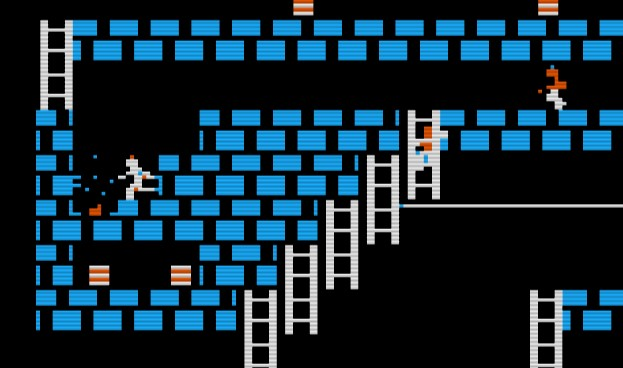
\includegraphics[width=\columnwidth]{digging}
\end{center}

The {\Tt{}\nwlinkedidentq{DIG{\_}DIRECTION}{NW1Xx3lK-10jlgu-c}\nwendquote} location stores which direction we're digging in, and the {\Tt{}DIG{\_}ANIM{\_}STATE\nwendquote}
location stores how far along in the 13-step animation cycle we are.

\nwenddocs{}\nwbegincode{436}\sublabel{NW1Xx3lK-10jlgu-c}\nwmargintag{{\nwtagstyle{}\subpageref{NW1Xx3lK-10jlgu-c}}}\moddef{defines~{\nwtagstyle{}\subpageref{NW1Xx3lK-10jlgu-1}}}\plusendmoddef\nwstartdeflinemarkup\nwusesondefline{\\{NW1Xx3lK-1p0Y9w-1}}\nwprevnextdefs{NW1Xx3lK-10jlgu-b}{NW1Xx3lK-10jlgu-d}\nwenddeflinemarkup
\nwlinkedidentc{DIG_DIRECTION}{NW1Xx3lK-10jlgu-c}       EQU     $9C     ; 0xFF = left, 0x00 = not digging, 0x01 = right
DIG_ANIM_STATE      EQU     $A0     ; 00-0C
\nwindexdefn{\nwixident{DIG{\_}DIRECTION}}{DIG:unDIRECTION}{NW1Xx3lK-10jlgu-c}\eatline
\nwused{\\{NW1Xx3lK-1p0Y9w-1}}\nwidentdefs{\\{{\nwixident{DIG{\_}DIRECTION}}{DIG:unDIRECTION}}}\nwendcode{}\nwbegindocs{437}\nwdocspar
The {\Tt{}\nwlinkedidentq{DIG{\_}DEBRIS{\_}LEFT{\_}SPRITES}{NW1Xx3lK-1W8AJS-M}\nwendquote}, {\Tt{}\nwlinkedidentq{DIG{\_}DEBRIS{\_}RIGHT{\_}SPRITES}{NW1Xx3lK-1W8AJS-M}\nwendquote} and {\Tt{}\nwlinkedidentq{DIG{\_}BRICK{\_}SPRITES}{NW1Xx3lK-1W8AJS-M}\nwendquote} tables
contain the sprites used during
the animation. There's also a little sequence of notes that plays while digging, given by
{\Tt{}\nwlinkedidentq{DIG{\_}NOTE{\_}PITCHES}{NW1Xx3lK-1W8AJS-M}\nwendquote} and {\Tt{}\nwlinkedidentq{DIG{\_}NOTE{\_}DURATIONS}{NW1Xx3lK-1W8AJS-M}\nwendquote}.

\nwenddocs{}\nwbegincode{438}\sublabel{NW1Xx3lK-1W8AJS-M}\nwmargintag{{\nwtagstyle{}\subpageref{NW1Xx3lK-1W8AJS-M}}}\moddef{tables~{\nwtagstyle{}\subpageref{NW1Xx3lK-1W8AJS-1}}}\plusendmoddef\nwstartdeflinemarkup\nwusesondefline{\\{NW1Xx3lK-1p0Y9w-1}}\nwprevnextdefs{NW1Xx3lK-1W8AJS-L}{NW1Xx3lK-1W8AJS-N}\nwenddeflinemarkup
    ORG     $697A
\nwlinkedidentc{DIG_DEBRIS_LEFT_SPRITES}{NW1Xx3lK-1W8AJS-M}:
    HEX     1B 1B 1C 1C 1D 1D 1E 1E 00 00 00 00
\nwlinkedidentc{DIG_DEBRIS_RIGHT_SPRITES}{NW1Xx3lK-1W8AJS-M}:
    HEX     26 26 27 27 1D 1D 1E 1E 00 00 00 00
\nwlinkedidentc{DIG_BRICK_SPRITES}{NW1Xx3lK-1W8AJS-M}:
    HEX     1F 1F 20 20 21 21 22 22 23 23 24 24
\nwlinkedidentc{DIG_NOTE_PITCHES}{NW1Xx3lK-1W8AJS-M}:
    HEX     20 20 20 20 20 20 20 20 24 24 24 24 24
\nwlinkedidentc{DIG_NOTE_DURATIONS}{NW1Xx3lK-1W8AJS-M}:
    HEX     04 04 04 04 04 04 04 04 03 03 02 02 01
\nwindexdefn{\nwixident{DIG{\_}NOTE{\_}PITCHES}}{DIG:unNOTE:unPITCHES}{NW1Xx3lK-1W8AJS-M}\nwindexdefn{\nwixident{DIG{\_}NOTE{\_}DURATIONS}}{DIG:unNOTE:unDURATIONS}{NW1Xx3lK-1W8AJS-M}\nwindexdefn{\nwixident{DIG{\_}DEBRIS{\_}LEFT{\_}SPRITES}}{DIG:unDEBRIS:unLEFT:unSPRITES}{NW1Xx3lK-1W8AJS-M}\nwindexdefn{\nwixident{DIG{\_}DEBRIS{\_}RIGHT{\_}SPRITES}}{DIG:unDEBRIS:unRIGHT:unSPRITES}{NW1Xx3lK-1W8AJS-M}\nwindexdefn{\nwixident{DIG{\_}BRICK{\_}SPRITES}}{DIG:unBRICK:unSPRITES}{NW1Xx3lK-1W8AJS-M}\eatline
\nwused{\\{NW1Xx3lK-1p0Y9w-1}}\nwidentdefs{\\{{\nwixident{DIG{\_}BRICK{\_}SPRITES}}{DIG:unBRICK:unSPRITES}}\\{{\nwixident{DIG{\_}DEBRIS{\_}LEFT{\_}SPRITES}}{DIG:unDEBRIS:unLEFT:unSPRITES}}\\{{\nwixident{DIG{\_}DEBRIS{\_}RIGHT{\_}SPRITES}}{DIG:unDEBRIS:unRIGHT:unSPRITES}}\\{{\nwixident{DIG{\_}NOTE{\_}DURATIONS}}{DIG:unNOTE:unDURATIONS}}\\{{\nwixident{DIG{\_}NOTE{\_}PITCHES}}{DIG:unNOTE:unPITCHES}}}\nwendcode{}\nwbegindocs{439}\nwdocspar
The player cannot dig to the left if they're on the bottom-most row or the leftmost column,
or if there's no brick below and to the left. Also, there has to be nothing to the left
of the player.

\nwenddocs{}\nwbegincode{440}\sublabel{NW1Xx3lK-FL5jU-1}\nwmargintag{{\nwtagstyle{}\subpageref{NW1Xx3lK-FL5jU-1}}}\moddef{try digging left~{\nwtagstyle{}\subpageref{NW1Xx3lK-FL5jU-1}}}\endmoddef\nwstartdeflinemarkup\nwusesondefline{\\{NW1Xx3lK-8jv1b-C}}\nwenddeflinemarkup
    ORG     $67D8
    SUBROUTINE

.cannot_dig_:
    JMP     .stop_digging

\nwlinkedidentc{TRY_DIGGING_LEFT}{NW1Xx3lK-FL5jU-1}:
    LDA     #$FF
    STA     \nwlinkedidentc{DIG_DIRECTION}{NW1Xx3lK-10jlgu-c}
    STA     \nwlinkedidentc{KEY_COMMAND}{NW1Xx3lK-10jlgu-a}
    STA     \nwlinkedidentc{KEY_COMMAND_LR}{NW1Xx3lK-10jlgu-a}      ; \nwlinkedidentc{DIG_DIRECTION}{NW1Xx3lK-10jlgu-c} = KEY_COMMANDs = 0xFF
    LDA     #$00
    STA     DIG_ANIM_STATE      ; DIG_ANIM_STATE = 0

TRY_DIGGING_LEFT_check_can_dig_left:
    LDY     \nwlinkedidentc{PLAYER_ROW}{NW1Xx3lK-10jlgu-M}
    CPY     #MAX_GAME_ROW
    BCS     .cannot_dig_        ; row >= 15, so cannot dig.

    INY
    JSR     \nwlinkedidentc{GET_PTRS_TO_CURR_LEVEL_SPRITE_DATA}{NW1Xx3lK-3AYvuG-1}
    LDY     \nwlinkedidentc{PLAYER_COL}{NW1Xx3lK-10jlgu-M}
    BEQ     .cannot_dig_        ; col == 0, so cannot dig left.

    DEY
    LDA     (\nwlinkedidentc{PTR1}{NW1Xx3lK-10jlgu-L}),Y
    CMP     #SPRITE_BRICK
    BNE     .cannot_dig_        ; no brick below and to the left, so cannot dig left.

    LDY     \nwlinkedidentc{PLAYER_ROW}{NW1Xx3lK-10jlgu-M}
    JSR     \nwlinkedidentc{GET_PTRS_TO_CURR_LEVEL_SPRITE_DATA}{NW1Xx3lK-3AYvuG-1}
    LDY     \nwlinkedidentc{PLAYER_COL}{NW1Xx3lK-10jlgu-M}
    DEY
    LDA     (\nwlinkedidentc{PTR1}{NW1Xx3lK-10jlgu-L}),Y
    CMP     #SPRITE_EMPTY
    BNE     .not_empty_to_left  ; not empty to the left, so maybe cannot dig left.

    ; Can dig!
    JSR     \nwlinkedidentc{GET_SPRITE_AND_SCREEN_COORD_AT_PLAYER}{NW1Xx3lK-24XK8J-1}
    JSR     \nwlinkedidentc{ERASE_SPRITE_AT_PIXEL_COORDS}{NW1Xx3lK-xFyle-1}
    JSR     \nwlinkedidentc{NUDGE_PLAYER_TOWARDS_EXACT_COLUMN}{NW1Xx3lK-PXGvu-1}
    JSR     \nwlinkedidentc{NUDGE_PLAYER_TOWARDS_EXACT_ROW}{NW1Xx3lK-PXGvu-1}
    LDY     DIG_ANIM_STATE
    LDA     \nwlinkedidentc{DIG_NOTE_PITCHES}{NW1Xx3lK-1W8AJS-M},Y
    LDX     \nwlinkedidentc{DIG_NOTE_DURATIONS}{NW1Xx3lK-1W8AJS-M},Y
    JSR     \nwlinkedidentc{APPEND_NOTE}{NW1Xx3lK-4JsOpf-1}

    LDX     DIG_ANIM_STATE
    LDA     #$00                ; running left
    CPX     #$06
    BCS     .note_0             ; DIG_ANIM_STATE >= 6
    LDA     #$06                ; digging left
.note_0:
    STA     \nwlinkedidentc{PLAYER_ANIM_STATE}{NW1Xx3lK-10jlgu-P}
    JSR     \nwlinkedidentc{DRAW_PLAYER}{NW1Xx3lK-2x2oAB-1}

    LDX     DIG_ANIM_STATE
    CPX     #$0C
    BEQ     .move_player_left
    CPX     #$00
    BEQ     .draw_curr_dig              ; Don't have to erase previous dig debris sprite

    ; Erase the previous dig debris sprite
    LDA     \nwlinkedidentc{DIG_DEBRIS_LEFT_SPRITES}{NW1Xx3lK-1W8AJS-M}-1,X
    PHA
    LDX     \nwlinkedidentc{PLAYER_COL}{NW1Xx3lK-10jlgu-M}
    DEX
    LDY     \nwlinkedidentc{PLAYER_ROW}{NW1Xx3lK-10jlgu-M}
    JSR     \nwlinkedidentc{GET_SCREEN_COORDS_FOR}{NW1Xx3lK-8jv1b-5}
    PLA
    JSR     \nwlinkedidentc{ERASE_SPRITE_AT_PIXEL_COORDS}{NW1Xx3lK-xFyle-1}

    LDX     DIG_ANIM_STATE
.draw_curr_dig:
    LDA     \nwlinkedidentc{DIG_DEBRIS_LEFT_SPRITES}{NW1Xx3lK-1W8AJS-M},X
    PHA
    LDX     \nwlinkedidentc{PLAYER_COL}{NW1Xx3lK-10jlgu-M}
    DEX
    STX     \nwlinkedidentc{GAME_COLNUM}{NW1Xx3lK-10jlgu-7}
    LDY     \nwlinkedidentc{PLAYER_ROW}{NW1Xx3lK-10jlgu-M}
    STY     \nwlinkedidentc{GAME_ROWNUM}{NW1Xx3lK-10jlgu-7}
    JSR     \nwlinkedidentc{GET_SCREEN_COORDS_FOR}{NW1Xx3lK-8jv1b-5}
    PLA
    JSR     \nwlinkedidentc{DRAW_SPRITE_AT_PIXEL_COORDS}{NW1Xx3lK-30KKiv-1}     ; Draw current dig debris sprite above dig site

    LDX     DIG_ANIM_STATE
    LDA     \nwlinkedidentc{DIG_BRICK_SPRITES}{NW1Xx3lK-1W8AJS-M},X
    INC     \nwlinkedidentc{GAME_ROWNUM}{NW1Xx3lK-10jlgu-7}
    JSR     \nwlinkedidentc{DRAW_SPRITE_PAGE1}{NW1Xx3lK-8jv1b-A}               ; Draw dig brick sprite at dig site

    INC     DIG_ANIM_STATE
    CLC
    RTS

.not_empty_to_left:
    LDY     \nwlinkedidentc{PLAYER_ROW}{NW1Xx3lK-10jlgu-M}
    INY
    STY     \nwlinkedidentc{GAME_ROWNUM}{NW1Xx3lK-10jlgu-7}
    LDY     \nwlinkedidentc{PLAYER_COL}{NW1Xx3lK-10jlgu-M}
    DEY
    STY     \nwlinkedidentc{GAME_COLNUM}{NW1Xx3lK-10jlgu-7}
    LDA     #SPRITE_BRICK
    JSR     \nwlinkedidentc{DRAW_SPRITE_PAGE1}{NW1Xx3lK-8jv1b-A}           ; Draw brick below and to the left of player

    LDX     DIG_ANIM_STATE
    BEQ     .stop_digging

    ; Erase previous dig debris sprite
    DEX
    LDA     \nwlinkedidentc{DIG_DEBRIS_LEFT_SPRITES}{NW1Xx3lK-1W8AJS-M},X
    PHA
    LDY     \nwlinkedidentc{PLAYER_ROW}{NW1Xx3lK-10jlgu-M}
    LDX     \nwlinkedidentc{PLAYER_COL}{NW1Xx3lK-10jlgu-M}
    DEX
    JSR     \nwlinkedidentc{GET_SCREEN_COORDS_FOR}{NW1Xx3lK-8jv1b-5}
    PLA
    JSR     \nwlinkedidentc{ERASE_SPRITE_AT_PIXEL_COORDS}{NW1Xx3lK-xFyle-1}

.stop_digging:
    LDA     #$00
    STA     \nwlinkedidentc{DIG_DIRECTION}{NW1Xx3lK-10jlgu-c}
    SEC
    RTS

.move_player_left:
    LDX     \nwlinkedidentc{PLAYER_COL}{NW1Xx3lK-10jlgu-M}
    DEX
    JMP     \nwlinkedidentc{DROP_PLAYER_IN_HOLE}{NW1Xx3lK-3DiAjH-1}
\nwindexdefn{\nwixident{TRY{\_}DIGGING{\_}LEFT}}{TRY:unDIGGING:unLEFT}{NW1Xx3lK-FL5jU-1}\eatline
\nwused{\\{NW1Xx3lK-8jv1b-C}}\nwidentdefs{\\{{\nwixident{TRY{\_}DIGGING{\_}LEFT}}{TRY:unDIGGING:unLEFT}}}\nwidentuses{\\{{\nwixident{APPEND{\_}NOTE}}{APPEND:unNOTE}}\\{{\nwixident{DIG{\_}BRICK{\_}SPRITES}}{DIG:unBRICK:unSPRITES}}\\{{\nwixident{DIG{\_}DEBRIS{\_}LEFT{\_}SPRITES}}{DIG:unDEBRIS:unLEFT:unSPRITES}}\\{{\nwixident{DIG{\_}DIRECTION}}{DIG:unDIRECTION}}\\{{\nwixident{DIG{\_}NOTE{\_}DURATIONS}}{DIG:unNOTE:unDURATIONS}}\\{{\nwixident{DIG{\_}NOTE{\_}PITCHES}}{DIG:unNOTE:unPITCHES}}\\{{\nwixident{DRAW{\_}PLAYER}}{DRAW:unPLAYER}}\\{{\nwixident{DRAW{\_}SPRITE{\_}AT{\_}PIXEL{\_}COORDS}}{DRAW:unSPRITE:unAT:unPIXEL:unCOORDS}}\\{{\nwixident{DRAW{\_}SPRITE{\_}PAGE1}}{DRAW:unSPRITE:unPAGE1}}\\{{\nwixident{DROP{\_}PLAYER{\_}IN{\_}HOLE}}{DROP:unPLAYER:unIN:unHOLE}}\\{{\nwixident{ERASE{\_}SPRITE{\_}AT{\_}PIXEL{\_}COORDS}}{ERASE:unSPRITE:unAT:unPIXEL:unCOORDS}}\\{{\nwixident{GAME{\_}COLNUM}}{GAME:unCOLNUM}}\\{{\nwixident{GAME{\_}ROWNUM}}{GAME:unROWNUM}}\\{{\nwixident{GET{\_}PTRS{\_}TO{\_}CURR{\_}LEVEL{\_}SPRITE{\_}DATA}}{GET:unPTRS:unTO:unCURR:unLEVEL:unSPRITE:unDATA}}\\{{\nwixident{GET{\_}SCREEN{\_}COORDS{\_}FOR}}{GET:unSCREEN:unCOORDS:unFOR}}\\{{\nwixident{GET{\_}SPRITE{\_}AND{\_}SCREEN{\_}COORD{\_}AT{\_}PLAYER}}{GET:unSPRITE:unAND:unSCREEN:unCOORD:unAT:unPLAYER}}\\{{\nwixident{KEY{\_}COMMAND}}{KEY:unCOMMAND}}\\{{\nwixident{KEY{\_}COMMAND{\_}LR}}{KEY:unCOMMAND:unLR}}\\{{\nwixident{NUDGE{\_}PLAYER{\_}TOWARDS{\_}EXACT{\_}COLUMN}}{NUDGE:unPLAYER:unTOWARDS:unEXACT:unCOLUMN}}\\{{\nwixident{NUDGE{\_}PLAYER{\_}TOWARDS{\_}EXACT{\_}ROW}}{NUDGE:unPLAYER:unTOWARDS:unEXACT:unROW}}\\{{\nwixident{PLAYER{\_}ANIM{\_}STATE}}{PLAYER:unANIM:unSTATE}}\\{{\nwixident{PLAYER{\_}COL}}{PLAYER:unCOL}}\\{{\nwixident{PLAYER{\_}ROW}}{PLAYER:unROW}}\\{{\nwixident{PTR1}}{PTR1}}}\nwindexuse{\nwixident{APPEND{\_}NOTE}}{APPEND:unNOTE}{NW1Xx3lK-FL5jU-1}\nwindexuse{\nwixident{DIG{\_}BRICK{\_}SPRITES}}{DIG:unBRICK:unSPRITES}{NW1Xx3lK-FL5jU-1}\nwindexuse{\nwixident{DIG{\_}DEBRIS{\_}LEFT{\_}SPRITES}}{DIG:unDEBRIS:unLEFT:unSPRITES}{NW1Xx3lK-FL5jU-1}\nwindexuse{\nwixident{DIG{\_}DIRECTION}}{DIG:unDIRECTION}{NW1Xx3lK-FL5jU-1}\nwindexuse{\nwixident{DIG{\_}NOTE{\_}DURATIONS}}{DIG:unNOTE:unDURATIONS}{NW1Xx3lK-FL5jU-1}\nwindexuse{\nwixident{DIG{\_}NOTE{\_}PITCHES}}{DIG:unNOTE:unPITCHES}{NW1Xx3lK-FL5jU-1}\nwindexuse{\nwixident{DRAW{\_}PLAYER}}{DRAW:unPLAYER}{NW1Xx3lK-FL5jU-1}\nwindexuse{\nwixident{DRAW{\_}SPRITE{\_}AT{\_}PIXEL{\_}COORDS}}{DRAW:unSPRITE:unAT:unPIXEL:unCOORDS}{NW1Xx3lK-FL5jU-1}\nwindexuse{\nwixident{DRAW{\_}SPRITE{\_}PAGE1}}{DRAW:unSPRITE:unPAGE1}{NW1Xx3lK-FL5jU-1}\nwindexuse{\nwixident{DROP{\_}PLAYER{\_}IN{\_}HOLE}}{DROP:unPLAYER:unIN:unHOLE}{NW1Xx3lK-FL5jU-1}\nwindexuse{\nwixident{ERASE{\_}SPRITE{\_}AT{\_}PIXEL{\_}COORDS}}{ERASE:unSPRITE:unAT:unPIXEL:unCOORDS}{NW1Xx3lK-FL5jU-1}\nwindexuse{\nwixident{GAME{\_}COLNUM}}{GAME:unCOLNUM}{NW1Xx3lK-FL5jU-1}\nwindexuse{\nwixident{GAME{\_}ROWNUM}}{GAME:unROWNUM}{NW1Xx3lK-FL5jU-1}\nwindexuse{\nwixident{GET{\_}PTRS{\_}TO{\_}CURR{\_}LEVEL{\_}SPRITE{\_}DATA}}{GET:unPTRS:unTO:unCURR:unLEVEL:unSPRITE:unDATA}{NW1Xx3lK-FL5jU-1}\nwindexuse{\nwixident{GET{\_}SCREEN{\_}COORDS{\_}FOR}}{GET:unSCREEN:unCOORDS:unFOR}{NW1Xx3lK-FL5jU-1}\nwindexuse{\nwixident{GET{\_}SPRITE{\_}AND{\_}SCREEN{\_}COORD{\_}AT{\_}PLAYER}}{GET:unSPRITE:unAND:unSCREEN:unCOORD:unAT:unPLAYER}{NW1Xx3lK-FL5jU-1}\nwindexuse{\nwixident{KEY{\_}COMMAND}}{KEY:unCOMMAND}{NW1Xx3lK-FL5jU-1}\nwindexuse{\nwixident{KEY{\_}COMMAND{\_}LR}}{KEY:unCOMMAND:unLR}{NW1Xx3lK-FL5jU-1}\nwindexuse{\nwixident{NUDGE{\_}PLAYER{\_}TOWARDS{\_}EXACT{\_}COLUMN}}{NUDGE:unPLAYER:unTOWARDS:unEXACT:unCOLUMN}{NW1Xx3lK-FL5jU-1}\nwindexuse{\nwixident{NUDGE{\_}PLAYER{\_}TOWARDS{\_}EXACT{\_}ROW}}{NUDGE:unPLAYER:unTOWARDS:unEXACT:unROW}{NW1Xx3lK-FL5jU-1}\nwindexuse{\nwixident{PLAYER{\_}ANIM{\_}STATE}}{PLAYER:unANIM:unSTATE}{NW1Xx3lK-FL5jU-1}\nwindexuse{\nwixident{PLAYER{\_}COL}}{PLAYER:unCOL}{NW1Xx3lK-FL5jU-1}\nwindexuse{\nwixident{PLAYER{\_}ROW}}{PLAYER:unROW}{NW1Xx3lK-FL5jU-1}\nwindexuse{\nwixident{PTR1}}{PTR1}{NW1Xx3lK-FL5jU-1}\nwendcode{}\nwbegindocs{441}\nwdocspar
\nwenddocs{}\nwbegincode{442}\sublabel{NW1Xx3lK-2HpjFG-1}\nwmargintag{{\nwtagstyle{}\subpageref{NW1Xx3lK-2HpjFG-1}}}\moddef{try digging right~{\nwtagstyle{}\subpageref{NW1Xx3lK-2HpjFG-1}}}\endmoddef\nwstartdeflinemarkup\nwusesondefline{\\{NW1Xx3lK-8jv1b-C}}\nwenddeflinemarkup
    ORG     $689E
    SUBROUTINE

.cannot_dig_:
    JMP     .stop_digging

\nwlinkedidentc{TRY_DIGGING_RIGHT}{NW1Xx3lK-2HpjFG-1}:
    LDA     #$01
    STA     \nwlinkedidentc{DIG_DIRECTION}{NW1Xx3lK-10jlgu-c}
    STA     \nwlinkedidentc{KEY_COMMAND}{NW1Xx3lK-10jlgu-a}
    STA     \nwlinkedidentc{KEY_COMMAND_LR}{NW1Xx3lK-10jlgu-a}      ; \nwlinkedidentc{DIG_DIRECTION}{NW1Xx3lK-10jlgu-c} = KEY_COMMANDs = 0x01
    LDA     #$0C
    STA     DIG_ANIM_STATE      ; DIG_ANIM_STATE = 0x0C

TRY_DIGGING_RIGHT_check_can_dig_right:
    LDY     \nwlinkedidentc{PLAYER_ROW}{NW1Xx3lK-10jlgu-M}
    CPY     #MAX_GAME_ROW
    BCS     .cannot_dig_        ; row >= 15, so cannot dig.

    INY
    JSR     \nwlinkedidentc{GET_PTRS_TO_CURR_LEVEL_SPRITE_DATA}{NW1Xx3lK-3AYvuG-1}
    LDY     \nwlinkedidentc{PLAYER_COL}{NW1Xx3lK-10jlgu-M}
    CPY     #MAX_GAME_COL
    BCS     .cannot_dig_        ; col >= 27, so cannot dig right.

    INY
    LDA     (\nwlinkedidentc{PTR1}{NW1Xx3lK-10jlgu-L}),Y
    CMP     #SPRITE_BRICK
    BNE     .cannot_dig_        ; no brick below and to the right, so cannot dig right.

    LDY     \nwlinkedidentc{PLAYER_ROW}{NW1Xx3lK-10jlgu-M}
    JSR     \nwlinkedidentc{GET_PTRS_TO_CURR_LEVEL_SPRITE_DATA}{NW1Xx3lK-3AYvuG-1}
    LDY     \nwlinkedidentc{PLAYER_COL}{NW1Xx3lK-10jlgu-M}
    INY
    LDA     (\nwlinkedidentc{PTR1}{NW1Xx3lK-10jlgu-L}),Y
    CMP     #SPRITE_EMPTY
    BNE     .not_empty_to_right  ; not empty to the right, so maybe cannot dig right.

    ; Can dig!
    JSR     \nwlinkedidentc{GET_SPRITE_AND_SCREEN_COORD_AT_PLAYER}{NW1Xx3lK-24XK8J-1}
    JSR     \nwlinkedidentc{ERASE_SPRITE_AT_PIXEL_COORDS}{NW1Xx3lK-xFyle-1}
    JSR     \nwlinkedidentc{NUDGE_PLAYER_TOWARDS_EXACT_COLUMN}{NW1Xx3lK-PXGvu-1}
    JSR     \nwlinkedidentc{NUDGE_PLAYER_TOWARDS_EXACT_ROW}{NW1Xx3lK-PXGvu-1}
    LDY     DIG_ANIM_STATE
    LDA     \nwlinkedidentc{DIG_NOTE_PITCHES}{NW1Xx3lK-1W8AJS-M}-12,Y
    LDX     \nwlinkedidentc{DIG_NOTE_DURATIONS}{NW1Xx3lK-1W8AJS-M}-12,Y
    JSR     \nwlinkedidentc{APPEND_NOTE}{NW1Xx3lK-4JsOpf-1}

    LDX     DIG_ANIM_STATE
    LDA     #$08                ; running right
    CPX     #$12
    BCS     .note_0             ; DIG_ANIM_STATE >= 0x12
    LDA     #$0E                ; digging right
.note_0:
    STA     \nwlinkedidentc{PLAYER_ANIM_STATE}{NW1Xx3lK-10jlgu-P}
    JSR     \nwlinkedidentc{DRAW_PLAYER}{NW1Xx3lK-2x2oAB-1}

    LDX     DIG_ANIM_STATE
    CPX     #$18
    BEQ     .move_player_right
    CPX     #$0C
    BEQ     .draw_curr_dig              ; Don't have to erase previous dig debris sprite

    ; Erase the previous dig debris sprite
    LDA     \nwlinkedidentc{DIG_DEBRIS_LEFT_SPRITES}{NW1Xx3lK-1W8AJS-M}-1,X
    PHA
    LDX     \nwlinkedidentc{PLAYER_COL}{NW1Xx3lK-10jlgu-M}
    INX
    LDY     \nwlinkedidentc{PLAYER_ROW}{NW1Xx3lK-10jlgu-M}
    JSR     \nwlinkedidentc{GET_SCREEN_COORDS_FOR}{NW1Xx3lK-8jv1b-5}
    PLA
    JSR     \nwlinkedidentc{ERASE_SPRITE_AT_PIXEL_COORDS}{NW1Xx3lK-xFyle-1}

    LDX     DIG_ANIM_STATE
.draw_curr_dig:
    LDA     \nwlinkedidentc{DIG_DEBRIS_LEFT_SPRITES}{NW1Xx3lK-1W8AJS-M},X
    PHA
    LDX     \nwlinkedidentc{PLAYER_COL}{NW1Xx3lK-10jlgu-M}
    INX
    STX     \nwlinkedidentc{GAME_COLNUM}{NW1Xx3lK-10jlgu-7}
    LDY     \nwlinkedidentc{PLAYER_ROW}{NW1Xx3lK-10jlgu-M}
    STY     \nwlinkedidentc{GAME_ROWNUM}{NW1Xx3lK-10jlgu-7}
    JSR     \nwlinkedidentc{GET_SCREEN_COORDS_FOR}{NW1Xx3lK-8jv1b-5}
    PLA
    JSR     \nwlinkedidentc{DRAW_SPRITE_AT_PIXEL_COORDS}{NW1Xx3lK-30KKiv-1}     ; Draw current dig debris sprite above dig site

    INC     \nwlinkedidentc{GAME_ROWNUM}{NW1Xx3lK-10jlgu-7}
    LDX     DIG_ANIM_STATE
    LDA     \nwlinkedidentc{DIG_BRICK_SPRITES}{NW1Xx3lK-1W8AJS-M}-12,X
    JSR     \nwlinkedidentc{DRAW_SPRITE_PAGE1}{NW1Xx3lK-8jv1b-A}               ; Draw dig brick sprite at dig site

    INC     DIG_ANIM_STATE
    CLC
    RTS

.not_empty_to_right:
    LDY     \nwlinkedidentc{PLAYER_ROW}{NW1Xx3lK-10jlgu-M}
    INY
    STY     \nwlinkedidentc{GAME_ROWNUM}{NW1Xx3lK-10jlgu-7}
    LDY     \nwlinkedidentc{PLAYER_COL}{NW1Xx3lK-10jlgu-M}
    INY
    STY     \nwlinkedidentc{GAME_COLNUM}{NW1Xx3lK-10jlgu-7}
    LDA     #SPRITE_BRICK
    JSR     \nwlinkedidentc{DRAW_SPRITE_PAGE1}{NW1Xx3lK-8jv1b-A}           ; Draw brick below and to the right of player

    LDX     DIG_ANIM_STATE
    CPX     #$0C
    BEQ     .stop_digging

    ; Erase previous dig debris sprite
    DEX
    LDA     \nwlinkedidentc{DIG_DEBRIS_LEFT_SPRITES}{NW1Xx3lK-1W8AJS-M},X
    PHA
    LDX     \nwlinkedidentc{PLAYER_COL}{NW1Xx3lK-10jlgu-M}
    INX
    LDY     \nwlinkedidentc{PLAYER_ROW}{NW1Xx3lK-10jlgu-M}
    JSR     \nwlinkedidentc{GET_SCREEN_COORDS_FOR}{NW1Xx3lK-8jv1b-5}
    PLA
    JSR     \nwlinkedidentc{ERASE_SPRITE_AT_PIXEL_COORDS}{NW1Xx3lK-xFyle-1}

.stop_digging:
    LDA     #$00
    STA     \nwlinkedidentc{DIG_DIRECTION}{NW1Xx3lK-10jlgu-c}
    SEC
    RTS

.move_player_right:
    LDX     \nwlinkedidentc{PLAYER_COL}{NW1Xx3lK-10jlgu-M}
    INX
    JMP     \nwlinkedidentc{DROP_PLAYER_IN_HOLE}{NW1Xx3lK-3DiAjH-1}
\nwindexdefn{\nwixident{TRY{\_}DIGGING{\_}RIGHT}}{TRY:unDIGGING:unRIGHT}{NW1Xx3lK-2HpjFG-1}\eatline
\nwused{\\{NW1Xx3lK-8jv1b-C}}\nwidentdefs{\\{{\nwixident{TRY{\_}DIGGING{\_}RIGHT}}{TRY:unDIGGING:unRIGHT}}}\nwidentuses{\\{{\nwixident{APPEND{\_}NOTE}}{APPEND:unNOTE}}\\{{\nwixident{DIG{\_}BRICK{\_}SPRITES}}{DIG:unBRICK:unSPRITES}}\\{{\nwixident{DIG{\_}DEBRIS{\_}LEFT{\_}SPRITES}}{DIG:unDEBRIS:unLEFT:unSPRITES}}\\{{\nwixident{DIG{\_}DIRECTION}}{DIG:unDIRECTION}}\\{{\nwixident{DIG{\_}NOTE{\_}DURATIONS}}{DIG:unNOTE:unDURATIONS}}\\{{\nwixident{DIG{\_}NOTE{\_}PITCHES}}{DIG:unNOTE:unPITCHES}}\\{{\nwixident{DRAW{\_}PLAYER}}{DRAW:unPLAYER}}\\{{\nwixident{DRAW{\_}SPRITE{\_}AT{\_}PIXEL{\_}COORDS}}{DRAW:unSPRITE:unAT:unPIXEL:unCOORDS}}\\{{\nwixident{DRAW{\_}SPRITE{\_}PAGE1}}{DRAW:unSPRITE:unPAGE1}}\\{{\nwixident{DROP{\_}PLAYER{\_}IN{\_}HOLE}}{DROP:unPLAYER:unIN:unHOLE}}\\{{\nwixident{ERASE{\_}SPRITE{\_}AT{\_}PIXEL{\_}COORDS}}{ERASE:unSPRITE:unAT:unPIXEL:unCOORDS}}\\{{\nwixident{GAME{\_}COLNUM}}{GAME:unCOLNUM}}\\{{\nwixident{GAME{\_}ROWNUM}}{GAME:unROWNUM}}\\{{\nwixident{GET{\_}PTRS{\_}TO{\_}CURR{\_}LEVEL{\_}SPRITE{\_}DATA}}{GET:unPTRS:unTO:unCURR:unLEVEL:unSPRITE:unDATA}}\\{{\nwixident{GET{\_}SCREEN{\_}COORDS{\_}FOR}}{GET:unSCREEN:unCOORDS:unFOR}}\\{{\nwixident{GET{\_}SPRITE{\_}AND{\_}SCREEN{\_}COORD{\_}AT{\_}PLAYER}}{GET:unSPRITE:unAND:unSCREEN:unCOORD:unAT:unPLAYER}}\\{{\nwixident{KEY{\_}COMMAND}}{KEY:unCOMMAND}}\\{{\nwixident{KEY{\_}COMMAND{\_}LR}}{KEY:unCOMMAND:unLR}}\\{{\nwixident{NUDGE{\_}PLAYER{\_}TOWARDS{\_}EXACT{\_}COLUMN}}{NUDGE:unPLAYER:unTOWARDS:unEXACT:unCOLUMN}}\\{{\nwixident{NUDGE{\_}PLAYER{\_}TOWARDS{\_}EXACT{\_}ROW}}{NUDGE:unPLAYER:unTOWARDS:unEXACT:unROW}}\\{{\nwixident{PLAYER{\_}ANIM{\_}STATE}}{PLAYER:unANIM:unSTATE}}\\{{\nwixident{PLAYER{\_}COL}}{PLAYER:unCOL}}\\{{\nwixident{PLAYER{\_}ROW}}{PLAYER:unROW}}\\{{\nwixident{PTR1}}{PTR1}}}\nwindexuse{\nwixident{APPEND{\_}NOTE}}{APPEND:unNOTE}{NW1Xx3lK-2HpjFG-1}\nwindexuse{\nwixident{DIG{\_}BRICK{\_}SPRITES}}{DIG:unBRICK:unSPRITES}{NW1Xx3lK-2HpjFG-1}\nwindexuse{\nwixident{DIG{\_}DEBRIS{\_}LEFT{\_}SPRITES}}{DIG:unDEBRIS:unLEFT:unSPRITES}{NW1Xx3lK-2HpjFG-1}\nwindexuse{\nwixident{DIG{\_}DIRECTION}}{DIG:unDIRECTION}{NW1Xx3lK-2HpjFG-1}\nwindexuse{\nwixident{DIG{\_}NOTE{\_}DURATIONS}}{DIG:unNOTE:unDURATIONS}{NW1Xx3lK-2HpjFG-1}\nwindexuse{\nwixident{DIG{\_}NOTE{\_}PITCHES}}{DIG:unNOTE:unPITCHES}{NW1Xx3lK-2HpjFG-1}\nwindexuse{\nwixident{DRAW{\_}PLAYER}}{DRAW:unPLAYER}{NW1Xx3lK-2HpjFG-1}\nwindexuse{\nwixident{DRAW{\_}SPRITE{\_}AT{\_}PIXEL{\_}COORDS}}{DRAW:unSPRITE:unAT:unPIXEL:unCOORDS}{NW1Xx3lK-2HpjFG-1}\nwindexuse{\nwixident{DRAW{\_}SPRITE{\_}PAGE1}}{DRAW:unSPRITE:unPAGE1}{NW1Xx3lK-2HpjFG-1}\nwindexuse{\nwixident{DROP{\_}PLAYER{\_}IN{\_}HOLE}}{DROP:unPLAYER:unIN:unHOLE}{NW1Xx3lK-2HpjFG-1}\nwindexuse{\nwixident{ERASE{\_}SPRITE{\_}AT{\_}PIXEL{\_}COORDS}}{ERASE:unSPRITE:unAT:unPIXEL:unCOORDS}{NW1Xx3lK-2HpjFG-1}\nwindexuse{\nwixident{GAME{\_}COLNUM}}{GAME:unCOLNUM}{NW1Xx3lK-2HpjFG-1}\nwindexuse{\nwixident{GAME{\_}ROWNUM}}{GAME:unROWNUM}{NW1Xx3lK-2HpjFG-1}\nwindexuse{\nwixident{GET{\_}PTRS{\_}TO{\_}CURR{\_}LEVEL{\_}SPRITE{\_}DATA}}{GET:unPTRS:unTO:unCURR:unLEVEL:unSPRITE:unDATA}{NW1Xx3lK-2HpjFG-1}\nwindexuse{\nwixident{GET{\_}SCREEN{\_}COORDS{\_}FOR}}{GET:unSCREEN:unCOORDS:unFOR}{NW1Xx3lK-2HpjFG-1}\nwindexuse{\nwixident{GET{\_}SPRITE{\_}AND{\_}SCREEN{\_}COORD{\_}AT{\_}PLAYER}}{GET:unSPRITE:unAND:unSCREEN:unCOORD:unAT:unPLAYER}{NW1Xx3lK-2HpjFG-1}\nwindexuse{\nwixident{KEY{\_}COMMAND}}{KEY:unCOMMAND}{NW1Xx3lK-2HpjFG-1}\nwindexuse{\nwixident{KEY{\_}COMMAND{\_}LR}}{KEY:unCOMMAND:unLR}{NW1Xx3lK-2HpjFG-1}\nwindexuse{\nwixident{NUDGE{\_}PLAYER{\_}TOWARDS{\_}EXACT{\_}COLUMN}}{NUDGE:unPLAYER:unTOWARDS:unEXACT:unCOLUMN}{NW1Xx3lK-2HpjFG-1}\nwindexuse{\nwixident{NUDGE{\_}PLAYER{\_}TOWARDS{\_}EXACT{\_}ROW}}{NUDGE:unPLAYER:unTOWARDS:unEXACT:unROW}{NW1Xx3lK-2HpjFG-1}\nwindexuse{\nwixident{PLAYER{\_}ANIM{\_}STATE}}{PLAYER:unANIM:unSTATE}{NW1Xx3lK-2HpjFG-1}\nwindexuse{\nwixident{PLAYER{\_}COL}}{PLAYER:unCOL}{NW1Xx3lK-2HpjFG-1}\nwindexuse{\nwixident{PLAYER{\_}ROW}}{PLAYER:unROW}{NW1Xx3lK-2HpjFG-1}\nwindexuse{\nwixident{PTR1}}{PTR1}{NW1Xx3lK-2HpjFG-1}\nwendcode{}\nwbegindocs{443}\nwdocspar
\nwenddocs{}\nwbegincode{444}\sublabel{NW1Xx3lK-3DiAjH-1}\nwmargintag{{\nwtagstyle{}\subpageref{NW1Xx3lK-3DiAjH-1}}}\moddef{drop player in hole~{\nwtagstyle{}\subpageref{NW1Xx3lK-3DiAjH-1}}}\endmoddef\nwstartdeflinemarkup\nwusesondefline{\\{NW1Xx3lK-8jv1b-C}}\nwenddeflinemarkup
    ORG     $6C39
\nwlinkedidentc{DROP_PLAYER_IN_HOLE}{NW1Xx3lK-3DiAjH-1}:
    SUBROUTINE

    LDA     #$00
    STA     \nwlinkedidentc{DIG_DIRECTION}{NW1Xx3lK-10jlgu-c}       ; Stop digging

    LDY     \nwlinkedidentc{PLAYER_ROW}{NW1Xx3lK-10jlgu-M}
    INY                         ; Move player down

    STX     \nwlinkedidentc{GAME_COLNUM}{NW1Xx3lK-10jlgu-7}
    STY     \nwlinkedidentc{GAME_ROWNUM}{NW1Xx3lK-10jlgu-7}
    \LA{}set active row pointer \code{}PTR1\edoc{} for \code{}Y\edoc{}~{\nwtagstyle{}\subpageref{NW1Xx3lK-qxK9U-1}}\RA{}
    LDA     #SPRITE_EMPTY
    LDY     \nwlinkedidentc{GAME_COLNUM}{NW1Xx3lK-10jlgu-7}
    STA     (\nwlinkedidentc{PTR1}{NW1Xx3lK-10jlgu-L}),Y                ; Set blank sprite at player location in active page
    JSR     \nwlinkedidentc{DRAW_SPRITE_PAGE1}{NW1Xx3lK-8jv1b-A}
    LDA     #SPRITE_EMPTY
    JSR     \nwlinkedidentc{DRAW_SPRITE_PAGE2}{NW1Xx3lK-8jv1b-A}       ; Draw blank at player location on both graphics pages

    DEC     \nwlinkedidentc{GAME_ROWNUM}{NW1Xx3lK-10jlgu-7}
    LDA     #SPRITE_EMPTY
    JSR     \nwlinkedidentc{DRAW_SPRITE_PAGE1}{NW1Xx3lK-8jv1b-A}       ; Draw blank at location above player
    INC     \nwlinkedidentc{GAME_ROWNUM}{NW1Xx3lK-10jlgu-7}
    LDX     #$FF

.loop:
    INX
    CPX     #$1E
    BEQ     .end
    LDA     BRICK_FILL_TIMERS,X
    BNE     .loop

    LDA     \nwlinkedidentc{GAME_ROWNUM}{NW1Xx3lK-10jlgu-7}
    STA     BRICK_DIG_ROWS,X
    LDA     \nwlinkedidentc{GAME_COLNUM}{NW1Xx3lK-10jlgu-7}
    STA     BRICK_DIG_COLS,X
    LDA     #$B4
    STA     BRICK_FILL_TIMERS,X
    SEC

.end:
    RTS
\nwindexdefn{\nwixident{DROP{\_}PLAYER{\_}IN{\_}HOLE}}{DROP:unPLAYER:unIN:unHOLE}{NW1Xx3lK-3DiAjH-1}\eatline
\nwused{\\{NW1Xx3lK-8jv1b-C}}\nwidentdefs{\\{{\nwixident{DROP{\_}PLAYER{\_}IN{\_}HOLE}}{DROP:unPLAYER:unIN:unHOLE}}}\nwidentuses{\\{{\nwixident{DIG{\_}DIRECTION}}{DIG:unDIRECTION}}\\{{\nwixident{DRAW{\_}SPRITE{\_}PAGE1}}{DRAW:unSPRITE:unPAGE1}}\\{{\nwixident{DRAW{\_}SPRITE{\_}PAGE2}}{DRAW:unSPRITE:unPAGE2}}\\{{\nwixident{GAME{\_}COLNUM}}{GAME:unCOLNUM}}\\{{\nwixident{GAME{\_}ROWNUM}}{GAME:unROWNUM}}\\{{\nwixident{PLAYER{\_}ROW}}{PLAYER:unROW}}\\{{\nwixident{PTR1}}{PTR1}}}\nwindexuse{\nwixident{DIG{\_}DIRECTION}}{DIG:unDIRECTION}{NW1Xx3lK-3DiAjH-1}\nwindexuse{\nwixident{DRAW{\_}SPRITE{\_}PAGE1}}{DRAW:unSPRITE:unPAGE1}{NW1Xx3lK-3DiAjH-1}\nwindexuse{\nwixident{DRAW{\_}SPRITE{\_}PAGE2}}{DRAW:unSPRITE:unPAGE2}{NW1Xx3lK-3DiAjH-1}\nwindexuse{\nwixident{GAME{\_}COLNUM}}{GAME:unCOLNUM}{NW1Xx3lK-3DiAjH-1}\nwindexuse{\nwixident{GAME{\_}ROWNUM}}{GAME:unROWNUM}{NW1Xx3lK-3DiAjH-1}\nwindexuse{\nwixident{PLAYER{\_}ROW}}{PLAYER:unROW}{NW1Xx3lK-3DiAjH-1}\nwindexuse{\nwixident{PTR1}}{PTR1}{NW1Xx3lK-3DiAjH-1}\nwendcode{}\nwbegindocs{445}\nwdocspar
The {\Tt{}\nwlinkedidentq{MOVE{\_}PLAYER}{NW1Xx3lK-1viPAs-1}\nwendquote} routine handle continuation of digging, player falling, and player keyboard input.

\nwenddocs{}\nwbegincode{446}\sublabel{NW1Xx3lK-1viPAs-1}\nwmargintag{{\nwtagstyle{}\subpageref{NW1Xx3lK-1viPAs-1}}}\moddef{move player~{\nwtagstyle{}\subpageref{NW1Xx3lK-1viPAs-1}}}\endmoddef\nwstartdeflinemarkup\nwusesondefline{\\{NW1Xx3lK-8jv1b-C}}\nwenddeflinemarkup
    ORG     $64BD
\nwlinkedidentc{MOVE_PLAYER}{NW1Xx3lK-1viPAs-1}:
    SUBROUTINE

    LDA     #$01
    STA     \nwlinkedidentc{DIDNT_PICK_UP_GOLD}{NW1Xx3lK-10jlgu-Z}   ; Reset \nwlinkedidentc{DIDNT_PICK_UP_GOLD}{NW1Xx3lK-10jlgu-Z}

    ; If we're digging, see if we can keep digging.
    LDA     \nwlinkedidentc{DIG_DIRECTION}{NW1Xx3lK-10jlgu-c}
    BEQ     .not_digging
    BPL     .digging_right
    JMP     TRY_DIGGING_LEFT_check_can_dig_left

.digging_right:
    JMP     TRY_DIGGING_RIGHT_check_can_dig_right

.not_digging:
    LDY     \nwlinkedidentc{PLAYER_ROW}{NW1Xx3lK-10jlgu-M}
    \LA{}set background row pointer \code{}PTR2\edoc{} for \code{}Y\edoc{}~{\nwtagstyle{}\subpageref{NW1Xx3lK-45yBRu-1}}\RA{}
    LDY     \nwlinkedidentc{PLAYER_COL}{NW1Xx3lK-10jlgu-M}
    LDA     (\nwlinkedidentc{PTR2}{NW1Xx3lK-10jlgu-L}),Y
    CMP     #SPRITE_LADDER
    BEQ     .check_for_keyboard_input_      ; ladder at background location?
    CMP     #SPRITE_ROPE
    BNE     .check_if_player_should_fall    ; rope at background location?
    LDA     \nwlinkedidentc{PLAYER_Y_ADJ}{NW1Xx3lK-10jlgu-P}
    CMP     #$02
    BEQ     .check_for_keyboard_input_      ; player at exact sprite row?

    ; player is not on exact sprite row, fallthrough.

.check_if_player_should_fall:
    LDA     \nwlinkedidentc{PLAYER_Y_ADJ}{NW1Xx3lK-10jlgu-P}
    CMP     #$02
    BCC     .make_player_fall               ; player slightly above sprite row?

    LDY     \nwlinkedidentc{PLAYER_ROW}{NW1Xx3lK-10jlgu-M}
    CPY     #MAX_GAME_ROW
    BEQ     .check_for_keyboard_input_      ; player exactly sprite row 15?

    ; Check the sprite at the player location
    \LA{}set active and background row pointers \code{}PTR1\edoc{} and \code{}PTR2\edoc{} for \code{}Y+1\edoc{}~{\nwtagstyle{}\subpageref{NW1Xx3lK-rGo92-1}}\RA{}

    LDY     \nwlinkedidentc{PLAYER_COL}{NW1Xx3lK-10jlgu-M}
    LDA     (\nwlinkedidentc{PTR1}{NW1Xx3lK-10jlgu-L}),Y
    CMP     #SPRITE_EMPTY
    BEQ     .make_player_fall
    CMP     #SPRITE_GUARD
    BEQ     .check_for_keyboard_input_
    LDA     (\nwlinkedidentc{PTR2}{NW1Xx3lK-10jlgu-L}),Y
    CMP     #SPRITE_BRICK
    BEQ     .check_for_keyboard_input_
    CMP     #SPRITE_STONE
    BEQ     .check_for_keyboard_input_
    CMP     #SPRITE_LADDER
    BNE     .make_player_fall

.check_for_keyboard_input_:
    JMP     .check_for_keyboard_input

.make_player_fall:
    LDA     #$00
    STA     $9B                     ; $9B = 0
    JSR     \nwlinkedidentc{GET_SPRITE_AND_SCREEN_COORD_AT_PLAYER}{NW1Xx3lK-24XK8J-1}
    JSR     \nwlinkedidentc{ERASE_SPRITE_AT_PIXEL_COORDS}{NW1Xx3lK-xFyle-1}

    LDA     #$07                    ; Next anim state: player falling, facing left
    LDX     PLAYER_FACING_DIRECTION
    BMI     .player_facing_left
    LDA     #$0F                    ; Next anim state: player falling, facing right
.player_facing_left:
    STA     \nwlinkedidentc{PLAYER_ANIM_STATE}{NW1Xx3lK-10jlgu-P}

    JSR     \nwlinkedidentc{NUDGE_PLAYER_TOWARDS_EXACT_COLUMN}{NW1Xx3lK-PXGvu-1}

    INC     \nwlinkedidentc{PLAYER_Y_ADJ}{NW1Xx3lK-10jlgu-P}            ; Move down one
    LDA     \nwlinkedidentc{PLAYER_Y_ADJ}{NW1Xx3lK-10jlgu-P}
    CMP     #$05
    BCS     .adjustment_overflow

    JSR     \nwlinkedidentc{CHECK_FOR_GOLD_PICKED_UP_BY_PLAYER}{NW1Xx3lK-2zzVjv-1}
    JMP     \nwlinkedidentc{DRAW_PLAYER}{NW1Xx3lK-2x2oAB-1}            ; tailcall

.adjustment_overflow:
    LDA     #$00
    STA     \nwlinkedidentc{PLAYER_Y_ADJ}{NW1Xx3lK-10jlgu-P}            ; Set vertical adjust to -2

    LDY     \nwlinkedidentc{PLAYER_ROW}{NW1Xx3lK-10jlgu-M}
    \LA{}set active and background row pointers \code{}PTR1\edoc{} and \code{}PTR2\edoc{} for \code{}Y\edoc{}~{\nwtagstyle{}\subpageref{NW1Xx3lK-4cENZH-1}}\RA{}
    LDY     \nwlinkedidentc{PLAYER_COL}{NW1Xx3lK-10jlgu-M}
    LDA     (\nwlinkedidentc{PTR2}{NW1Xx3lK-10jlgu-L}),Y
    CMP     #SPRITE_BRICK
    BNE     .set_on_level
    LDA     #SPRITE_EMPTY
.set_on_level:
    STA     (\nwlinkedidentc{PTR1}{NW1Xx3lK-10jlgu-L}),Y
    INC     \nwlinkedidentc{PLAYER_ROW}{NW1Xx3lK-10jlgu-M}          ; Move down
    LDY     \nwlinkedidentc{PLAYER_ROW}{NW1Xx3lK-10jlgu-M}
    \LA{}set active row pointer \code{}PTR1\edoc{} for \code{}Y\edoc{}~{\nwtagstyle{}\subpageref{NW1Xx3lK-qxK9U-1}}\RA{}

    LDY     \nwlinkedidentc{PLAYER_COL}{NW1Xx3lK-10jlgu-M}
    LDA     #SPRITE_PLAYER
    STA     (\nwlinkedidentc{PTR1}{NW1Xx3lK-10jlgu-L}),Y
    JMP     \nwlinkedidentc{DRAW_PLAYER}{NW1Xx3lK-2x2oAB-1}     ; tailcall

.check_for_keyboard_input:
    LDA     $9B
    BNE     .check_for_key  ; $9B doesn't play note
    LDA     #$64
    LDX     #$08
    JSR     \nwlinkedidentc{PLAY_NOTE}{NW1Xx3lK-1Ew0EG-1}       ; play note, pitch 0x64, duration 8.

.check_for_key:
    LDA     #$20
    STA     $A4
    STA     $9B
    JSR     \nwlinkedidentc{CHECK_FOR_INPUT}{NW1Xx3lK-1FsAoS-1}
    LDA     \nwlinkedidentc{KEY_COMMAND}{NW1Xx3lK-10jlgu-a}
    CMP     #$C9            ; 'I'
    BNE     .check_for_K
    JSR     \nwlinkedidentc{TRY_MOVING_UP}{NW1Xx3lK-PXGvu-2}
    BCS     .check_for_J    ; couldn't move up
    RTS

.check_for_K:
    CMP     #$CB            ; 'K'
    BNE     .check_for_U
    JSR     \nwlinkedidentc{TRY_MOVING_DOWN}{NW1Xx3lK-3I7nQV-1}
    BCS     .check_for_J
    RTS

.check_for_U:
    CMP     #$D5            ; 'U'
    BNE     .check_for_O
    JSR     \nwlinkedidentc{TRY_DIGGING_LEFT}{NW1Xx3lK-FL5jU-1}
    BCS     .check_for_J
    RTS

.check_for_O:
    CMP     #$CF            ; 'O'
    BNE     .check_for_J
    JSR     \nwlinkedidentc{TRY_DIGGING_RIGHT}{NW1Xx3lK-2HpjFG-1}
    BCS     .check_for_J
    RTS

.check_for_J:
    LDA     \nwlinkedidentc{KEY_COMMAND_LR}{NW1Xx3lK-10jlgu-a}
    CMP     #$CA            ; 'J'
    BNE     .check_for_L
    JMP     \nwlinkedidentc{TRY_MOVING_LEFT}{NW1Xx3lK-443qw5-1}

.check_for_L:
    CMP     #$CC            ; 'L'
    BNE     .end
    JMP     \nwlinkedidentc{TRY_MOVING_RIGHT}{NW1Xx3lK-2fpnEm-1}

.end:
    RTS
\nwindexdefn{\nwixident{MOVE{\_}PLAYER}}{MOVE:unPLAYER}{NW1Xx3lK-1viPAs-1}\eatline
\nwused{\\{NW1Xx3lK-8jv1b-C}}\nwidentdefs{\\{{\nwixident{MOVE{\_}PLAYER}}{MOVE:unPLAYER}}}\nwidentuses{\\{{\nwixident{CHECK{\_}FOR{\_}GOLD{\_}PICKED{\_}UP{\_}BY{\_}PLAYER}}{CHECK:unFOR:unGOLD:unPICKED:unUP:unBY:unPLAYER}}\\{{\nwixident{CHECK{\_}FOR{\_}INPUT}}{CHECK:unFOR:unINPUT}}\\{{\nwixident{DIDNT{\_}PICK{\_}UP{\_}GOLD}}{DIDNT:unPICK:unUP:unGOLD}}\\{{\nwixident{DIG{\_}DIRECTION}}{DIG:unDIRECTION}}\\{{\nwixident{DRAW{\_}PLAYER}}{DRAW:unPLAYER}}\\{{\nwixident{ERASE{\_}SPRITE{\_}AT{\_}PIXEL{\_}COORDS}}{ERASE:unSPRITE:unAT:unPIXEL:unCOORDS}}\\{{\nwixident{GET{\_}SPRITE{\_}AND{\_}SCREEN{\_}COORD{\_}AT{\_}PLAYER}}{GET:unSPRITE:unAND:unSCREEN:unCOORD:unAT:unPLAYER}}\\{{\nwixident{KEY{\_}COMMAND}}{KEY:unCOMMAND}}\\{{\nwixident{KEY{\_}COMMAND{\_}LR}}{KEY:unCOMMAND:unLR}}\\{{\nwixident{NUDGE{\_}PLAYER{\_}TOWARDS{\_}EXACT{\_}COLUMN}}{NUDGE:unPLAYER:unTOWARDS:unEXACT:unCOLUMN}}\\{{\nwixident{PLAY{\_}NOTE}}{PLAY:unNOTE}}\\{{\nwixident{PLAYER{\_}ANIM{\_}STATE}}{PLAYER:unANIM:unSTATE}}\\{{\nwixident{PLAYER{\_}COL}}{PLAYER:unCOL}}\\{{\nwixident{PLAYER{\_}ROW}}{PLAYER:unROW}}\\{{\nwixident{PLAYER{\_}Y{\_}ADJ}}{PLAYER:unY:unADJ}}\\{{\nwixident{PTR1}}{PTR1}}\\{{\nwixident{PTR2}}{PTR2}}\\{{\nwixident{TRY{\_}DIGGING{\_}LEFT}}{TRY:unDIGGING:unLEFT}}\\{{\nwixident{TRY{\_}DIGGING{\_}RIGHT}}{TRY:unDIGGING:unRIGHT}}\\{{\nwixident{TRY{\_}MOVING{\_}DOWN}}{TRY:unMOVING:unDOWN}}\\{{\nwixident{TRY{\_}MOVING{\_}LEFT}}{TRY:unMOVING:unLEFT}}\\{{\nwixident{TRY{\_}MOVING{\_}RIGHT}}{TRY:unMOVING:unRIGHT}}\\{{\nwixident{TRY{\_}MOVING{\_}UP}}{TRY:unMOVING:unUP}}}\nwindexuse{\nwixident{CHECK{\_}FOR{\_}GOLD{\_}PICKED{\_}UP{\_}BY{\_}PLAYER}}{CHECK:unFOR:unGOLD:unPICKED:unUP:unBY:unPLAYER}{NW1Xx3lK-1viPAs-1}\nwindexuse{\nwixident{CHECK{\_}FOR{\_}INPUT}}{CHECK:unFOR:unINPUT}{NW1Xx3lK-1viPAs-1}\nwindexuse{\nwixident{DIDNT{\_}PICK{\_}UP{\_}GOLD}}{DIDNT:unPICK:unUP:unGOLD}{NW1Xx3lK-1viPAs-1}\nwindexuse{\nwixident{DIG{\_}DIRECTION}}{DIG:unDIRECTION}{NW1Xx3lK-1viPAs-1}\nwindexuse{\nwixident{DRAW{\_}PLAYER}}{DRAW:unPLAYER}{NW1Xx3lK-1viPAs-1}\nwindexuse{\nwixident{ERASE{\_}SPRITE{\_}AT{\_}PIXEL{\_}COORDS}}{ERASE:unSPRITE:unAT:unPIXEL:unCOORDS}{NW1Xx3lK-1viPAs-1}\nwindexuse{\nwixident{GET{\_}SPRITE{\_}AND{\_}SCREEN{\_}COORD{\_}AT{\_}PLAYER}}{GET:unSPRITE:unAND:unSCREEN:unCOORD:unAT:unPLAYER}{NW1Xx3lK-1viPAs-1}\nwindexuse{\nwixident{KEY{\_}COMMAND}}{KEY:unCOMMAND}{NW1Xx3lK-1viPAs-1}\nwindexuse{\nwixident{KEY{\_}COMMAND{\_}LR}}{KEY:unCOMMAND:unLR}{NW1Xx3lK-1viPAs-1}\nwindexuse{\nwixident{NUDGE{\_}PLAYER{\_}TOWARDS{\_}EXACT{\_}COLUMN}}{NUDGE:unPLAYER:unTOWARDS:unEXACT:unCOLUMN}{NW1Xx3lK-1viPAs-1}\nwindexuse{\nwixident{PLAY{\_}NOTE}}{PLAY:unNOTE}{NW1Xx3lK-1viPAs-1}\nwindexuse{\nwixident{PLAYER{\_}ANIM{\_}STATE}}{PLAYER:unANIM:unSTATE}{NW1Xx3lK-1viPAs-1}\nwindexuse{\nwixident{PLAYER{\_}COL}}{PLAYER:unCOL}{NW1Xx3lK-1viPAs-1}\nwindexuse{\nwixident{PLAYER{\_}ROW}}{PLAYER:unROW}{NW1Xx3lK-1viPAs-1}\nwindexuse{\nwixident{PLAYER{\_}Y{\_}ADJ}}{PLAYER:unY:unADJ}{NW1Xx3lK-1viPAs-1}\nwindexuse{\nwixident{PTR1}}{PTR1}{NW1Xx3lK-1viPAs-1}\nwindexuse{\nwixident{PTR2}}{PTR2}{NW1Xx3lK-1viPAs-1}\nwindexuse{\nwixident{TRY{\_}DIGGING{\_}LEFT}}{TRY:unDIGGING:unLEFT}{NW1Xx3lK-1viPAs-1}\nwindexuse{\nwixident{TRY{\_}DIGGING{\_}RIGHT}}{TRY:unDIGGING:unRIGHT}{NW1Xx3lK-1viPAs-1}\nwindexuse{\nwixident{TRY{\_}MOVING{\_}DOWN}}{TRY:unMOVING:unDOWN}{NW1Xx3lK-1viPAs-1}\nwindexuse{\nwixident{TRY{\_}MOVING{\_}LEFT}}{TRY:unMOVING:unLEFT}{NW1Xx3lK-1viPAs-1}\nwindexuse{\nwixident{TRY{\_}MOVING{\_}RIGHT}}{TRY:unMOVING:unRIGHT}{NW1Xx3lK-1viPAs-1}\nwindexuse{\nwixident{TRY{\_}MOVING{\_}UP}}{TRY:unMOVING:unUP}{NW1Xx3lK-1viPAs-1}\nwendcode{}\nwbegindocs{447}\nwdocspar
{\Tt{}\nwlinkedidentq{ENABLE{\_}NEXT{\_}LEVEL{\_}LADDERS}{NW1Xx3lK-on53h-1}\nwendquote} goes through the registered ladder locations from last to first. Recall that
the ladder indices are 1-based, so that {\Tt{}LADDER{\_}LOCS{\_}[0]\nwendquote} does not contain ladder data. Instead,
that location is used as scratch space by this routine.

Recall also that {\Tt{}LADDER{\_}LOCS{\_}[X]\nwendquote} is negative if there is no ladder corresponding to entry {\Tt{}X\nwendquote}.

For each ladder, if there's a non-blank sprite on the background sprite page for it, we set
{\Tt{}\nwlinkedidentq{LADDER{\_}LOCS{\_}COL}{NW1Xx3lK-1W8AJS-D}\nwendquote} to {\Tt{}1\nwendquote}.

However, if there is a blank sprite on the background sprite page for it, then set it to the ladder
sprite, and if it's also blank on the active sprite page, set that to the ladder sprite, too. Then
draw the ladder on the background and active graphics pages, remove the ladder from the registered
locations, and keep going.

Once all ladder locations have been gone through, if {\Tt{}\nwlinkedidentq{LADDER{\_}LOCS{\_}COL}{NW1Xx3lK-1W8AJS-D}\nwendquote} is {\Tt{}1\nwendquote}---that is,
if there was a non-blank sprite on the background sprite page for any ladder location---then
decrement the gold count. Since this routine is only called when {\Tt{}\nwlinkedidentq{GOLD{\_}COUNT}{NW1Xx3lK-10jlgu-N}\nwendquote} is zero,
this sets {\Tt{}\nwlinkedidentq{GOLD{\_}COUNT}{NW1Xx3lK-10jlgu-N}\nwendquote} to {\Tt{}-1\nwendquote}.

\nwenddocs{}\nwbegincode{448}\sublabel{NW1Xx3lK-on53h-1}\nwmargintag{{\nwtagstyle{}\subpageref{NW1Xx3lK-on53h-1}}}\moddef{do ladders~{\nwtagstyle{}\subpageref{NW1Xx3lK-on53h-1}}}\endmoddef\nwstartdeflinemarkup\nwusesondefline{\\{NW1Xx3lK-8jv1b-C}}\nwenddeflinemarkup
    ORG     $8631
\nwlinkedidentc{ENABLE_NEXT_LEVEL_LADDERS}{NW1Xx3lK-on53h-1}:
    SUBROUTINE

    LDA     #$00
    STA     \nwlinkedidentc{LADDER_LOCS_COL}{NW1Xx3lK-1W8AJS-D}     ; \nwlinkedidentc{LADDER_LOCS_COL}{NW1Xx3lK-1W8AJS-D} = 0

    LDX     \nwlinkedidentc{LADDER_COUNT}{NW1Xx3lK-10jlgu-N}
    STX     .count              ; .count backwards from \nwlinkedidentc{LADDER_COUNT}{NW1Xx3lK-10jlgu-N} to 0
.loop:
    LDX     .count
    BEQ     .dec_gold_count_if_no_ladder

    LDA     \nwlinkedidentc{LADDER_LOCS_COL}{NW1Xx3lK-1W8AJS-D},X   ; A = \nwlinkedidentc{LADDER_LOCS_COL}{NW1Xx3lK-1W8AJS-D}[X]
    BMI     .next               ; If not present, next.

    STA     \nwlinkedidentc{GAME_COLNUM}{NW1Xx3lK-10jlgu-7}         ; \nwlinkedidentc{GAME_COLNUM}{NW1Xx3lK-10jlgu-7} = \nwlinkedidentc{LADDER_LOCS_COL}{NW1Xx3lK-1W8AJS-D}[X]
    LDA     \nwlinkedidentc{LADDER_LOCS_ROW}{NW1Xx3lK-1W8AJS-D},X
    STA     \nwlinkedidentc{GAME_ROWNUM}{NW1Xx3lK-10jlgu-7}         ; \nwlinkedidentc{GAME_ROWNUM}{NW1Xx3lK-10jlgu-7} = \nwlinkedidentc{LADDER_LOCS_ROW}{NW1Xx3lK-1W8AJS-D}[X]
    TAY
    \LA{}set active and background row pointers \code{}PTR1\edoc{} and \code{}PTR2\edoc{} for \code{}Y\edoc{}~{\nwtagstyle{}\subpageref{NW1Xx3lK-4cENZH-1}}\RA{}
    LDY     \nwlinkedidentc{GAME_COLNUM}{NW1Xx3lK-10jlgu-7}
    LDA     (\nwlinkedidentc{PTR2}{NW1Xx3lK-10jlgu-L}),Y            ; A = sprite at ladder loc
    BNE     .set_col_to_1

    LDA     #SPRITE_LADDER
    STA     (\nwlinkedidentc{PTR2}{NW1Xx3lK-10jlgu-L}),Y            ; Set background sprite to ladder
    LDA     (\nwlinkedidentc{PTR1}{NW1Xx3lK-10jlgu-L}),Y
    BNE     .draw_ladder        ; .draw_ladder if active sprite not blank

    LDA     #SPRITE_LADDER
    STA     (\nwlinkedidentc{PTR1}{NW1Xx3lK-10jlgu-L}),Y            ; Set active sprite to ladder

.draw_ladder:
    LDA     #SPRITE_LADDER
    JSR     \nwlinkedidentc{DRAW_SPRITE_PAGE2}{NW1Xx3lK-8jv1b-A}   ; Draw ladder on background page

    LDX     \nwlinkedidentc{GAME_COLNUM}{NW1Xx3lK-10jlgu-7}
    LDY     \nwlinkedidentc{GAME_ROWNUM}{NW1Xx3lK-10jlgu-7}
    JSR     \nwlinkedidentc{GET_SCREEN_COORDS_FOR}{NW1Xx3lK-8jv1b-5}
    LDA     #SPRITE_LADDER
    JSR     \nwlinkedidentc{DRAW_SPRITE_AT_PIXEL_COORDS}{NW1Xx3lK-30KKiv-1} ; Draw ladder on active page

    LDX     .count
    LDA     #$FF
    STA     \nwlinkedidentc{LADDER_LOCS_COL}{NW1Xx3lK-1W8AJS-D},X       ; Remove ladder loc
    BMI     .next                   ; Unconditional

.set_col_to_1:
    LDA     #$01
    STA     \nwlinkedidentc{LADDER_LOCS_COL}{NW1Xx3lK-1W8AJS-D}         ; \nwlinkedidentc{LADDER_LOCS_COL}{NW1Xx3lK-1W8AJS-D} = 1

.next:
    DEC     .count
    JMP     .loop

.dec_gold_count_if_no_ladder:
    LDA     \nwlinkedidentc{LADDER_LOCS_COL}{NW1Xx3lK-1W8AJS-D}
    BNE     .end
    DEC     \nwlinkedidentc{GOLD_COUNT}{NW1Xx3lK-10jlgu-N}

.end:
    RTS

.count:
    BYTE    0
\nwindexdefn{\nwixident{ENABLE{\_}NEXT{\_}LEVEL{\_}LADDERS}}{ENABLE:unNEXT:unLEVEL:unLADDERS}{NW1Xx3lK-on53h-1}\eatline
\nwused{\\{NW1Xx3lK-8jv1b-C}}\nwidentdefs{\\{{\nwixident{ENABLE{\_}NEXT{\_}LEVEL{\_}LADDERS}}{ENABLE:unNEXT:unLEVEL:unLADDERS}}}\nwidentuses{\\{{\nwixident{DRAW{\_}SPRITE{\_}AT{\_}PIXEL{\_}COORDS}}{DRAW:unSPRITE:unAT:unPIXEL:unCOORDS}}\\{{\nwixident{DRAW{\_}SPRITE{\_}PAGE2}}{DRAW:unSPRITE:unPAGE2}}\\{{\nwixident{GAME{\_}COLNUM}}{GAME:unCOLNUM}}\\{{\nwixident{GAME{\_}ROWNUM}}{GAME:unROWNUM}}\\{{\nwixident{GET{\_}SCREEN{\_}COORDS{\_}FOR}}{GET:unSCREEN:unCOORDS:unFOR}}\\{{\nwixident{GOLD{\_}COUNT}}{GOLD:unCOUNT}}\\{{\nwixident{LADDER{\_}COUNT}}{LADDER:unCOUNT}}\\{{\nwixident{LADDER{\_}LOCS{\_}COL}}{LADDER:unLOCS:unCOL}}\\{{\nwixident{LADDER{\_}LOCS{\_}ROW}}{LADDER:unLOCS:unROW}}\\{{\nwixident{PTR1}}{PTR1}}\\{{\nwixident{PTR2}}{PTR2}}}\nwindexuse{\nwixident{DRAW{\_}SPRITE{\_}AT{\_}PIXEL{\_}COORDS}}{DRAW:unSPRITE:unAT:unPIXEL:unCOORDS}{NW1Xx3lK-on53h-1}\nwindexuse{\nwixident{DRAW{\_}SPRITE{\_}PAGE2}}{DRAW:unSPRITE:unPAGE2}{NW1Xx3lK-on53h-1}\nwindexuse{\nwixident{GAME{\_}COLNUM}}{GAME:unCOLNUM}{NW1Xx3lK-on53h-1}\nwindexuse{\nwixident{GAME{\_}ROWNUM}}{GAME:unROWNUM}{NW1Xx3lK-on53h-1}\nwindexuse{\nwixident{GET{\_}SCREEN{\_}COORDS{\_}FOR}}{GET:unSCREEN:unCOORDS:unFOR}{NW1Xx3lK-on53h-1}\nwindexuse{\nwixident{GOLD{\_}COUNT}}{GOLD:unCOUNT}{NW1Xx3lK-on53h-1}\nwindexuse{\nwixident{LADDER{\_}COUNT}}{LADDER:unCOUNT}{NW1Xx3lK-on53h-1}\nwindexuse{\nwixident{LADDER{\_}LOCS{\_}COL}}{LADDER:unLOCS:unCOL}{NW1Xx3lK-on53h-1}\nwindexuse{\nwixident{LADDER{\_}LOCS{\_}ROW}}{LADDER:unLOCS:unROW}{NW1Xx3lK-on53h-1}\nwindexuse{\nwixident{PTR1}}{PTR1}{NW1Xx3lK-on53h-1}\nwindexuse{\nwixident{PTR2}}{PTR2}{NW1Xx3lK-on53h-1}\nwendcode{}\nwbegindocs{449}\nwdocspar
\chapter{Guard AI}

Like the player, each guard has a column and row sprite location and a horizontal and
vertical adjustment. Each guard also has an animation state and a facing direction.

Guards also maintain two timers: a gold timer and a resurrection timer. The resurrection timer
comes into play when a guard is killed by a closing hole.

\nwenddocs{}\nwbegincode{450}\sublabel{NW1Xx3lK-10jlgu-d}\nwmargintag{{\nwtagstyle{}\subpageref{NW1Xx3lK-10jlgu-d}}}\moddef{defines~{\nwtagstyle{}\subpageref{NW1Xx3lK-10jlgu-1}}}\plusendmoddef\nwstartdeflinemarkup\nwusesondefline{\\{NW1Xx3lK-1p0Y9w-1}}\nwprevnextdefs{NW1Xx3lK-10jlgu-c}{NW1Xx3lK-10jlgu-e}\nwenddeflinemarkup
\nwlinkedidentc{GUARD_LOCS_COL}{NW1Xx3lK-10jlgu-d}      EQU     $0C60       ; 8 bytes
\nwlinkedidentc{GUARD_LOCS_ROW}{NW1Xx3lK-10jlgu-d}      EQU     $0C68       ; 8 bytes
\nwlinkedidentc{GUARD_GOLD_TIMERS}{NW1Xx3lK-10jlgu-d}   EQU     $0C70       ; 8 bytes
\nwlinkedidentc{GUARD_X_ADJS}{NW1Xx3lK-10jlgu-d}        EQU     $0C78       ; 8 bytes
\nwlinkedidentc{GUARD_Y_ADJS}{NW1Xx3lK-10jlgu-d}        EQU     $0C80       ; 8 bytes
\nwlinkedidentc{GUARD_ANIM_STATES}{NW1Xx3lK-10jlgu-d}   EQU     $0C88       ; 8 bytes
\nwlinkedidentc{GUARD_FACING_DIRECTIONS}{NW1Xx3lK-10jlgu-d}     EQU     $0C90       ; 8 bytes
GUARD_RESURRECTION_TIMERS   EQU     $0C98       ; 8 bytes

\nwlinkedidentc{GUARD_LOC_COL}{NW1Xx3lK-10jlgu-d}       EQU     $12
\nwlinkedidentc{GUARD_LOC_ROW}{NW1Xx3lK-10jlgu-d}       EQU     $13
\nwlinkedidentc{GUARD_ANIM_STATE}{NW1Xx3lK-10jlgu-d}    EQU     $14
\nwlinkedidentc{GUARD_FACING_DIRECTION}{NW1Xx3lK-10jlgu-d}      EQU     $15     ; Hi bit set: facing left, otherwise facing right
\nwlinkedidentc{GUARD_GOLD_TIMER}{NW1Xx3lK-10jlgu-d}    EQU     $16
\nwlinkedidentc{GUARD_X_ADJ}{NW1Xx3lK-10jlgu-d}         EQU     $17
\nwlinkedidentc{GUARD_Y_ADJ}{NW1Xx3lK-10jlgu-d}         EQU     $18
\nwlinkedidentc{GUARD_NUM}{NW1Xx3lK-10jlgu-d}           EQU     $19

\nwlinkedidentc{GUARD_PATTERN}{NW1Xx3lK-10jlgu-d}       EQU     $63
\nwlinkedidentc{GUARD_PHASE}{NW1Xx3lK-10jlgu-d}         EQU     $64

GUARD_RESURRECT_COL EQU     $53
TMP_GUARD_COL       EQU     $55
TMP_GUARD_ROW       EQU     $56
\nwlinkedidentc{GUARD_GOLD_TIMER_START_VALUE}{NW1Xx3lK-10jlgu-d}        EQU     $5F
\nwindexdefn{\nwixident{GUARD{\_}LOCS{\_}COL}}{GUARD:unLOCS:unCOL}{NW1Xx3lK-10jlgu-d}\nwindexdefn{\nwixident{GUARD{\_}LOCS{\_}ROW}}{GUARD:unLOCS:unROW}{NW1Xx3lK-10jlgu-d}\nwindexdefn{\nwixident{GUARD{\_}GOLD{\_}TIMERS}}{GUARD:unGOLD:unTIMERS}{NW1Xx3lK-10jlgu-d}\nwindexdefn{\nwixident{GUARD{\_}X{\_}ADJS}}{GUARD:unX:unADJS}{NW1Xx3lK-10jlgu-d}\nwindexdefn{\nwixident{GUARD{\_}Y{\_}ADJS}}{GUARD:unY:unADJS}{NW1Xx3lK-10jlgu-d}\nwindexdefn{\nwixident{GUARD{\_}ANIM{\_}STATES}}{GUARD:unANIM:unSTATES}{NW1Xx3lK-10jlgu-d}\nwindexdefn{\nwixident{GUARD{\_}FACING{\_}DIRECTIONS}}{GUARD:unFACING:unDIRECTIONS}{NW1Xx3lK-10jlgu-d}\nwindexdefn{\nwixident{GUARD{\_}LOC{\_}COL}}{GUARD:unLOC:unCOL}{NW1Xx3lK-10jlgu-d}\nwindexdefn{\nwixident{GUARD{\_}LOC{\_}ROW}}{GUARD:unLOC:unROW}{NW1Xx3lK-10jlgu-d}\nwindexdefn{\nwixident{GUARD{\_}GOLD{\_}TIMER}}{GUARD:unGOLD:unTIMER}{NW1Xx3lK-10jlgu-d}\nwindexdefn{\nwixident{GUARD{\_}X{\_}ADJ}}{GUARD:unX:unADJ}{NW1Xx3lK-10jlgu-d}\nwindexdefn{\nwixident{GUARD{\_}Y{\_}ADJ}}{GUARD:unY:unADJ}{NW1Xx3lK-10jlgu-d}\nwindexdefn{\nwixident{GUARD{\_}ANIM{\_}STATE}}{GUARD:unANIM:unSTATE}{NW1Xx3lK-10jlgu-d}\nwindexdefn{\nwixident{GUARD{\_}FACING{\_}DIRECTION}}{GUARD:unFACING:unDIRECTION}{NW1Xx3lK-10jlgu-d}\nwindexdefn{\nwixident{GUARD{\_}NUM}}{GUARD:unNUM}{NW1Xx3lK-10jlgu-d}\nwindexdefn{\nwixident{GUARD{\_}PATTERN}}{GUARD:unPATTERN}{NW1Xx3lK-10jlgu-d}\nwindexdefn{\nwixident{GUARD{\_}PHASE}}{GUARD:unPHASE}{NW1Xx3lK-10jlgu-d}\nwindexdefn{\nwixident{GUARD{\_}GOLD{\_}TIMER{\_}START{\_}VALUE}}{GUARD:unGOLD:unTIMER:unSTART:unVALUE}{NW1Xx3lK-10jlgu-d}\eatline
\nwused{\\{NW1Xx3lK-1p0Y9w-1}}\nwidentdefs{\\{{\nwixident{GUARD{\_}ANIM{\_}STATE}}{GUARD:unANIM:unSTATE}}\\{{\nwixident{GUARD{\_}ANIM{\_}STATES}}{GUARD:unANIM:unSTATES}}\\{{\nwixident{GUARD{\_}FACING{\_}DIRECTION}}{GUARD:unFACING:unDIRECTION}}\\{{\nwixident{GUARD{\_}FACING{\_}DIRECTIONS}}{GUARD:unFACING:unDIRECTIONS}}\\{{\nwixident{GUARD{\_}GOLD{\_}TIMER}}{GUARD:unGOLD:unTIMER}}\\{{\nwixident{GUARD{\_}GOLD{\_}TIMER{\_}START{\_}VALUE}}{GUARD:unGOLD:unTIMER:unSTART:unVALUE}}\\{{\nwixident{GUARD{\_}GOLD{\_}TIMERS}}{GUARD:unGOLD:unTIMERS}}\\{{\nwixident{GUARD{\_}LOC{\_}COL}}{GUARD:unLOC:unCOL}}\\{{\nwixident{GUARD{\_}LOC{\_}ROW}}{GUARD:unLOC:unROW}}\\{{\nwixident{GUARD{\_}LOCS{\_}COL}}{GUARD:unLOCS:unCOL}}\\{{\nwixident{GUARD{\_}LOCS{\_}ROW}}{GUARD:unLOCS:unROW}}\\{{\nwixident{GUARD{\_}NUM}}{GUARD:unNUM}}\\{{\nwixident{GUARD{\_}PATTERN}}{GUARD:unPATTERN}}\\{{\nwixident{GUARD{\_}PHASE}}{GUARD:unPHASE}}\\{{\nwixident{GUARD{\_}X{\_}ADJ}}{GUARD:unX:unADJ}}\\{{\nwixident{GUARD{\_}X{\_}ADJS}}{GUARD:unX:unADJS}}\\{{\nwixident{GUARD{\_}Y{\_}ADJ}}{GUARD:unY:unADJ}}\\{{\nwixident{GUARD{\_}Y{\_}ADJS}}{GUARD:unY:unADJS}}}\nwendcode{}\nwbegindocs{451}\nwdocspar
\nwenddocs{}\nwbegincode{452}\sublabel{NW1Xx3lK-1W8AJS-N}\nwmargintag{{\nwtagstyle{}\subpageref{NW1Xx3lK-1W8AJS-N}}}\moddef{tables~{\nwtagstyle{}\subpageref{NW1Xx3lK-1W8AJS-1}}}\plusendmoddef\nwstartdeflinemarkup\nwusesondefline{\\{NW1Xx3lK-1p0Y9w-1}}\nwprevnextdefs{NW1Xx3lK-1W8AJS-M}{NW1Xx3lK-1W8AJS-O}\nwenddeflinemarkup
    ORG     $621D
\nwlinkedidentc{GUARD_GOLD_TIMER_START_VALUES}{NW1Xx3lK-1W8AJS-N}:
    HEX     26 26 2E 44 47 49 4A 4B 4C 4D 4E 4F 50
\nwindexdefn{\nwixident{GUARD{\_}GOLD{\_}TIMER{\_}START{\_}VALUES}}{GUARD:unGOLD:unTIMER:unSTART:unVALUES}{NW1Xx3lK-1W8AJS-N}\eatline
\nwused{\\{NW1Xx3lK-1p0Y9w-1}}\nwidentdefs{\\{{\nwixident{GUARD{\_}GOLD{\_}TIMER{\_}START{\_}VALUES}}{GUARD:unGOLD:unTIMER:unSTART:unVALUES}}}\nwendcode{}\nwbegindocs{453}\nwdocspar
\nwenddocs{}\nwbegincode{454}\sublabel{NW1Xx3lK-4Ue5BT-1}\nwmargintag{{\nwtagstyle{}\subpageref{NW1Xx3lK-4Ue5BT-1}}}\moddef{nudge guards~{\nwtagstyle{}\subpageref{NW1Xx3lK-4Ue5BT-1}}}\endmoddef\nwstartdeflinemarkup\nwusesondefline{\\{NW1Xx3lK-8jv1b-C}}\nwenddeflinemarkup
    ORG     $7582
\nwlinkedidentc{NUDGE_GUARD_TOWARDS_EXACT_COLUMN}{NW1Xx3lK-4Ue5BT-1}:
    SUBROUTINE

    LDA     \nwlinkedidentc{GUARD_X_ADJ}{NW1Xx3lK-10jlgu-d}
    CMP     #$02
    BCC     .slightly_left
    BEQ     .end

.slightly_right:
    DEC     \nwlinkedidentc{GUARD_X_ADJ}{NW1Xx3lK-10jlgu-d}        ; Nudge guard left
    JMP     \nwlinkedidentc{CHECK_FOR_GOLD_PICKED_UP_BY_GUARD}{NW1Xx3lK-46BTMv-1}

.slightly_left:
    INC     \nwlinkedidentc{GUARD_X_ADJ}{NW1Xx3lK-10jlgu-d}        ; Nudge guard right
    JMP     \nwlinkedidentc{CHECK_FOR_GOLD_PICKED_UP_BY_GUARD}{NW1Xx3lK-46BTMv-1}

.end:
    RTS

    ORG     $7595
\nwlinkedidentc{NUDGE_GUARD_TOWARDS_EXACT_ROW}{NW1Xx3lK-4Ue5BT-1}:
    SUBROUTINE

    LDA     \nwlinkedidentc{GUARD_Y_ADJ}{NW1Xx3lK-10jlgu-d}
    CMP     #$02
    BCC     .slightly_above
    BEQ     .end

.slightly_below:
    DEC     \nwlinkedidentc{GUARD_Y_ADJ}{NW1Xx3lK-10jlgu-d}        ; Nudge guard up
    JMP     \nwlinkedidentc{CHECK_FOR_GOLD_PICKED_UP_BY_GUARD}{NW1Xx3lK-46BTMv-1}

.slightly_above:
    INC     \nwlinkedidentc{GUARD_Y_ADJ}{NW1Xx3lK-10jlgu-d}        ; Nudge guard down
    JMP     \nwlinkedidentc{CHECK_FOR_GOLD_PICKED_UP_BY_GUARD}{NW1Xx3lK-46BTMv-1}

.end:
    RTS
\nwindexdefn{\nwixident{NUDGE{\_}GUARD{\_}TOWARDS{\_}EXACT{\_}COLUMN}}{NUDGE:unGUARD:unTOWARDS:unEXACT:unCOLUMN}{NW1Xx3lK-4Ue5BT-1}\nwindexdefn{\nwixident{NUDGE{\_}GUARD{\_}TOWARDS{\_}EXACT{\_}ROW}}{NUDGE:unGUARD:unTOWARDS:unEXACT:unROW}{NW1Xx3lK-4Ue5BT-1}\eatline
\nwused{\\{NW1Xx3lK-8jv1b-C}}\nwidentdefs{\\{{\nwixident{NUDGE{\_}GUARD{\_}TOWARDS{\_}EXACT{\_}COLUMN}}{NUDGE:unGUARD:unTOWARDS:unEXACT:unCOLUMN}}\\{{\nwixident{NUDGE{\_}GUARD{\_}TOWARDS{\_}EXACT{\_}ROW}}{NUDGE:unGUARD:unTOWARDS:unEXACT:unROW}}}\nwidentuses{\\{{\nwixident{CHECK{\_}FOR{\_}GOLD{\_}PICKED{\_}UP{\_}BY{\_}GUARD}}{CHECK:unFOR:unGOLD:unPICKED:unUP:unBY:unGUARD}}\\{{\nwixident{GUARD{\_}X{\_}ADJ}}{GUARD:unX:unADJ}}\\{{\nwixident{GUARD{\_}Y{\_}ADJ}}{GUARD:unY:unADJ}}}\nwindexuse{\nwixident{CHECK{\_}FOR{\_}GOLD{\_}PICKED{\_}UP{\_}BY{\_}GUARD}}{CHECK:unFOR:unGOLD:unPICKED:unUP:unBY:unGUARD}{NW1Xx3lK-4Ue5BT-1}\nwindexuse{\nwixident{GUARD{\_}X{\_}ADJ}}{GUARD:unX:unADJ}{NW1Xx3lK-4Ue5BT-1}\nwindexuse{\nwixident{GUARD{\_}Y{\_}ADJ}}{GUARD:unY:unADJ}{NW1Xx3lK-4Ue5BT-1}\nwendcode{}\nwbegindocs{455}\nwdocspar
If the guard is exactly on a sprite coordinate, and there's gold there, and
{\Tt{}\nwlinkedidentq{GUARD{\_}GOLD{\_}TIMER}{NW1Xx3lK-10jlgu-d}\nwendquote} is zero or positive, then set {\Tt{}\nwlinkedidentq{GUARD{\_}GOLD{\_}TIMER}{NW1Xx3lK-10jlgu-d}\nwendquote} to {\Tt{}0xFF\ -\ {\$}53\nwendquote},
and remove the gold.

\nwenddocs{}\nwbegincode{456}\sublabel{NW1Xx3lK-46BTMv-1}\nwmargintag{{\nwtagstyle{}\subpageref{NW1Xx3lK-46BTMv-1}}}\moddef{check for gold picked up by guard~{\nwtagstyle{}\subpageref{NW1Xx3lK-46BTMv-1}}}\endmoddef\nwstartdeflinemarkup\nwusesondefline{\\{NW1Xx3lK-8jv1b-C}}\nwenddeflinemarkup
    ORG     $74F7
\nwlinkedidentc{CHECK_FOR_GOLD_PICKED_UP_BY_GUARD}{NW1Xx3lK-46BTMv-1}:
    SUBROUTINE

    LDA     \nwlinkedidentc{GUARD_X_ADJ}{NW1Xx3lK-10jlgu-d}
    CMP     #$02
    BNE     .end
    LDA     \nwlinkedidentc{GUARD_Y_ADJ}{NW1Xx3lK-10jlgu-d}
    CMP     #$02
    BNE     .end

    LDY     \nwlinkedidentc{GUARD_LOC_ROW}{NW1Xx3lK-10jlgu-d}
    \LA{}set background row pointer \code{}PTR2\edoc{} for \code{}Y\edoc{}~{\nwtagstyle{}\subpageref{NW1Xx3lK-45yBRu-1}}\RA{}
    LDY     \nwlinkedidentc{GUARD_LOC_COL}{NW1Xx3lK-10jlgu-d}
    LDA     (\nwlinkedidentc{PTR2}{NW1Xx3lK-10jlgu-L}),Y

    CMP     #SPRITE_GOLD
    BNE     .end

    LDA     \nwlinkedidentc{GUARD_GOLD_TIMER}{NW1Xx3lK-10jlgu-d}        ; Does guard have gold already?
    BMI     .end

    LDA     #$FF
    SEC
    SBC     $53
    STA     \nwlinkedidentc{GUARD_GOLD_TIMER}{NW1Xx3lK-10jlgu-d}        ; \nwlinkedidentc{GUARD_GOLD_TIMER}{NW1Xx3lK-10jlgu-d} = 0xFF - $53

    ; Remove gold from screen
    LDA     #SPRITE_EMPTY
    STA     (\nwlinkedidentc{PTR2}{NW1Xx3lK-10jlgu-L}),Y
    LDY     \nwlinkedidentc{GUARD_LOC_ROW}{NW1Xx3lK-10jlgu-d}
    STY     \nwlinkedidentc{GAME_ROWNUM}{NW1Xx3lK-10jlgu-7}
    LDY     \nwlinkedidentc{GUARD_LOC_COL}{NW1Xx3lK-10jlgu-d}
    STY     \nwlinkedidentc{GAME_COLNUM}{NW1Xx3lK-10jlgu-7}
    JSR     \nwlinkedidentc{DRAW_SPRITE_PAGE2}{NW1Xx3lK-8jv1b-A}

    LDY     \nwlinkedidentc{GAME_ROWNUM}{NW1Xx3lK-10jlgu-7}
    LDX     \nwlinkedidentc{GAME_COLNUM}{NW1Xx3lK-10jlgu-7}
    JSR     \nwlinkedidentc{GET_SCREEN_COORDS_FOR}{NW1Xx3lK-8jv1b-5}
    LDA     #SPRITE_GOLD
    JMP     \nwlinkedidentc{ERASE_SPRITE_AT_PIXEL_COORDS}{NW1Xx3lK-xFyle-1}        ; tailcall

.end:
    RTS
\nwindexdefn{\nwixident{CHECK{\_}FOR{\_}GOLD{\_}PICKED{\_}UP{\_}BY{\_}GUARD}}{CHECK:unFOR:unGOLD:unPICKED:unUP:unBY:unGUARD}{NW1Xx3lK-46BTMv-1}\eatline
\nwused{\\{NW1Xx3lK-8jv1b-C}}\nwidentdefs{\\{{\nwixident{CHECK{\_}FOR{\_}GOLD{\_}PICKED{\_}UP{\_}BY{\_}GUARD}}{CHECK:unFOR:unGOLD:unPICKED:unUP:unBY:unGUARD}}}\nwidentuses{\\{{\nwixident{DRAW{\_}SPRITE{\_}PAGE2}}{DRAW:unSPRITE:unPAGE2}}\\{{\nwixident{ERASE{\_}SPRITE{\_}AT{\_}PIXEL{\_}COORDS}}{ERASE:unSPRITE:unAT:unPIXEL:unCOORDS}}\\{{\nwixident{GAME{\_}COLNUM}}{GAME:unCOLNUM}}\\{{\nwixident{GAME{\_}ROWNUM}}{GAME:unROWNUM}}\\{{\nwixident{GET{\_}SCREEN{\_}COORDS{\_}FOR}}{GET:unSCREEN:unCOORDS:unFOR}}\\{{\nwixident{GUARD{\_}GOLD{\_}TIMER}}{GUARD:unGOLD:unTIMER}}\\{{\nwixident{GUARD{\_}LOC{\_}COL}}{GUARD:unLOC:unCOL}}\\{{\nwixident{GUARD{\_}LOC{\_}ROW}}{GUARD:unLOC:unROW}}\\{{\nwixident{GUARD{\_}X{\_}ADJ}}{GUARD:unX:unADJ}}\\{{\nwixident{GUARD{\_}Y{\_}ADJ}}{GUARD:unY:unADJ}}\\{{\nwixident{PTR2}}{PTR2}}}\nwindexuse{\nwixident{DRAW{\_}SPRITE{\_}PAGE2}}{DRAW:unSPRITE:unPAGE2}{NW1Xx3lK-46BTMv-1}\nwindexuse{\nwixident{ERASE{\_}SPRITE{\_}AT{\_}PIXEL{\_}COORDS}}{ERASE:unSPRITE:unAT:unPIXEL:unCOORDS}{NW1Xx3lK-46BTMv-1}\nwindexuse{\nwixident{GAME{\_}COLNUM}}{GAME:unCOLNUM}{NW1Xx3lK-46BTMv-1}\nwindexuse{\nwixident{GAME{\_}ROWNUM}}{GAME:unROWNUM}{NW1Xx3lK-46BTMv-1}\nwindexuse{\nwixident{GET{\_}SCREEN{\_}COORDS{\_}FOR}}{GET:unSCREEN:unCOORDS:unFOR}{NW1Xx3lK-46BTMv-1}\nwindexuse{\nwixident{GUARD{\_}GOLD{\_}TIMER}}{GUARD:unGOLD:unTIMER}{NW1Xx3lK-46BTMv-1}\nwindexuse{\nwixident{GUARD{\_}LOC{\_}COL}}{GUARD:unLOC:unCOL}{NW1Xx3lK-46BTMv-1}\nwindexuse{\nwixident{GUARD{\_}LOC{\_}ROW}}{GUARD:unLOC:unROW}{NW1Xx3lK-46BTMv-1}\nwindexuse{\nwixident{GUARD{\_}X{\_}ADJ}}{GUARD:unX:unADJ}{NW1Xx3lK-46BTMv-1}\nwindexuse{\nwixident{GUARD{\_}Y{\_}ADJ}}{GUARD:unY:unADJ}{NW1Xx3lK-46BTMv-1}\nwindexuse{\nwixident{PTR2}}{PTR2}{NW1Xx3lK-46BTMv-1}\nwendcode{}\nwbegindocs{457}\nwdocspar
\nwenddocs{}\nwbegincode{458}\sublabel{NW1Xx3lK-2Q1NVC-1}\nwmargintag{{\nwtagstyle{}\subpageref{NW1Xx3lK-2Q1NVC-1}}}\moddef{increment guard animation state~{\nwtagstyle{}\subpageref{NW1Xx3lK-2Q1NVC-1}}}\endmoddef\nwstartdeflinemarkup\nwusesondefline{\\{NW1Xx3lK-8jv1b-C}}\nwenddeflinemarkup
    ORG     $7574
\nwlinkedidentc{INC_GUARD_ANIM_STATE}{NW1Xx3lK-2Q1NVC-1}:
    SUBROUTINE

    INC     \nwlinkedidentc{GUARD_ANIM_STATE}{NW1Xx3lK-10jlgu-d}
    CMP     \nwlinkedidentc{GUARD_ANIM_STATE}{NW1Xx3lK-10jlgu-d}
    BCC     .check_upper_bound      ; lower bound < \nwlinkedidentc{GUARD_ANIM_STATE}{NW1Xx3lK-10jlgu-d}?
    ; otherwise \nwlinkedidentc{PLAYER_ANIM_STATE}{NW1Xx3lK-10jlgu-P} <= lower bound:

.write_lower_bound:
    STA     \nwlinkedidentc{GUARD_ANIM_STATE}{NW1Xx3lK-10jlgu-d}       ; \nwlinkedidentc{GUARD_ANIM_STATE}{NW1Xx3lK-10jlgu-d} = lower bound
    RTS

.check_upper_bound:
    CPX     \nwlinkedidentc{GUARD_ANIM_STATE}{NW1Xx3lK-10jlgu-d}
    BCC     .write_lower_bound       ; \nwlinkedidentc{GUARD_ANIM_STATE}{NW1Xx3lK-10jlgu-d} > upper bound?
    ; otherwise \nwlinkedidentc{GUARD_ANIM_STATE}{NW1Xx3lK-10jlgu-d} <= upper bound:
    RTS
\nwindexdefn{\nwixident{INC{\_}GUARD{\_}ANIM{\_}STATE}}{INC:unGUARD:unANIM:unSTATE}{NW1Xx3lK-2Q1NVC-1}\eatline
\nwused{\\{NW1Xx3lK-8jv1b-C}}\nwidentdefs{\\{{\nwixident{INC{\_}GUARD{\_}ANIM{\_}STATE}}{INC:unGUARD:unANIM:unSTATE}}}\nwidentuses{\\{{\nwixident{GUARD{\_}ANIM{\_}STATE}}{GUARD:unANIM:unSTATE}}\\{{\nwixident{PLAYER{\_}ANIM{\_}STATE}}{PLAYER:unANIM:unSTATE}}}\nwindexuse{\nwixident{GUARD{\_}ANIM{\_}STATE}}{GUARD:unANIM:unSTATE}{NW1Xx3lK-2Q1NVC-1}\nwindexuse{\nwixident{PLAYER{\_}ANIM{\_}STATE}}{PLAYER:unANIM:unSTATE}{NW1Xx3lK-2Q1NVC-1}\nwendcode{}\nwbegindocs{459}\nwdocspar
\nwenddocs{}\nwbegincode{460}\sublabel{NW1Xx3lK-12rZGg-1}\nwmargintag{{\nwtagstyle{}\subpageref{NW1Xx3lK-12rZGg-1}}}\moddef{guard store and load data~{\nwtagstyle{}\subpageref{NW1Xx3lK-12rZGg-1}}}\endmoddef\nwstartdeflinemarkup\nwusesondefline{\\{NW1Xx3lK-8jv1b-C}}\nwenddeflinemarkup
    ORG     $75A8
\nwlinkedidentc{STORE_GUARD_DATA}{NW1Xx3lK-12rZGg-1}:
    SUBROUTINE

    LDX     \nwlinkedidentc{GUARD_NUM}{NW1Xx3lK-10jlgu-d}
    LDA     \nwlinkedidentc{GUARD_LOC_COL}{NW1Xx3lK-10jlgu-d}
    STA     \nwlinkedidentc{GUARD_LOCS_COL}{NW1Xx3lK-10jlgu-d},X
    LDA     \nwlinkedidentc{GUARD_LOC_ROW}{NW1Xx3lK-10jlgu-d}
    STA     \nwlinkedidentc{GUARD_LOCS_ROW}{NW1Xx3lK-10jlgu-d},X
    LDA     \nwlinkedidentc{GUARD_X_ADJ}{NW1Xx3lK-10jlgu-d}
    STA     \nwlinkedidentc{GUARD_X_ADJS}{NW1Xx3lK-10jlgu-d},X
    LDA     \nwlinkedidentc{GUARD_Y_ADJ}{NW1Xx3lK-10jlgu-d}
    STA     \nwlinkedidentc{GUARD_Y_ADJS}{NW1Xx3lK-10jlgu-d},X
    LDA     \nwlinkedidentc{GUARD_GOLD_TIMER}{NW1Xx3lK-10jlgu-d}
    STA     \nwlinkedidentc{GUARD_GOLD_TIMERS}{NW1Xx3lK-10jlgu-d},X
    LDA     \nwlinkedidentc{GUARD_FACING_DIRECTION}{NW1Xx3lK-10jlgu-d}
    STA     \nwlinkedidentc{GUARD_FACING_DIRECTIONS}{NW1Xx3lK-10jlgu-d},X
    LDA     \nwlinkedidentc{GUARD_ANIM_STATE}{NW1Xx3lK-10jlgu-d}
    STA     \nwlinkedidentc{GUARD_ANIM_STATES}{NW1Xx3lK-10jlgu-d},X
    RTS

\nwlinkedidentc{LOAD_GUARD_DATA}{NW1Xx3lK-12rZGg-1}:
    SUBROUTINE

    LDX     \nwlinkedidentc{GUARD_NUM}{NW1Xx3lK-10jlgu-d}
    LDA     \nwlinkedidentc{GUARD_LOCS_COL}{NW1Xx3lK-10jlgu-d},X
    STA     \nwlinkedidentc{GUARD_LOC_COL}{NW1Xx3lK-10jlgu-d}
    LDA     \nwlinkedidentc{GUARD_LOCS_ROW}{NW1Xx3lK-10jlgu-d},X
    STA     \nwlinkedidentc{GUARD_LOC_ROW}{NW1Xx3lK-10jlgu-d}
    LDA     \nwlinkedidentc{GUARD_X_ADJS}{NW1Xx3lK-10jlgu-d},X
    STA     \nwlinkedidentc{GUARD_X_ADJ}{NW1Xx3lK-10jlgu-d}
    LDA     \nwlinkedidentc{GUARD_Y_ADJS}{NW1Xx3lK-10jlgu-d},X
    STA     \nwlinkedidentc{GUARD_Y_ADJ}{NW1Xx3lK-10jlgu-d}
    LDA     \nwlinkedidentc{GUARD_ANIM_STATES}{NW1Xx3lK-10jlgu-d},X
    STA     \nwlinkedidentc{GUARD_ANIM_STATE}{NW1Xx3lK-10jlgu-d}
    LDA     \nwlinkedidentc{GUARD_FACING_DIRECTIONS}{NW1Xx3lK-10jlgu-d},X
    STA     \nwlinkedidentc{GUARD_FACING_DIRECTION}{NW1Xx3lK-10jlgu-d}
    LDA     \nwlinkedidentc{GUARD_GOLD_TIMERS}{NW1Xx3lK-10jlgu-d},X
    STA     \nwlinkedidentc{GUARD_GOLD_TIMER}{NW1Xx3lK-10jlgu-d}
    RTS
\nwindexdefn{\nwixident{STORE{\_}GUARD{\_}DATA}}{STORE:unGUARD:unDATA}{NW1Xx3lK-12rZGg-1}\nwindexdefn{\nwixident{LOAD{\_}GUARD{\_}DATA}}{LOAD:unGUARD:unDATA}{NW1Xx3lK-12rZGg-1}\eatline
\nwused{\\{NW1Xx3lK-8jv1b-C}}\nwidentdefs{\\{{\nwixident{LOAD{\_}GUARD{\_}DATA}}{LOAD:unGUARD:unDATA}}\\{{\nwixident{STORE{\_}GUARD{\_}DATA}}{STORE:unGUARD:unDATA}}}\nwidentuses{\\{{\nwixident{GUARD{\_}ANIM{\_}STATE}}{GUARD:unANIM:unSTATE}}\\{{\nwixident{GUARD{\_}ANIM{\_}STATES}}{GUARD:unANIM:unSTATES}}\\{{\nwixident{GUARD{\_}FACING{\_}DIRECTION}}{GUARD:unFACING:unDIRECTION}}\\{{\nwixident{GUARD{\_}FACING{\_}DIRECTIONS}}{GUARD:unFACING:unDIRECTIONS}}\\{{\nwixident{GUARD{\_}GOLD{\_}TIMER}}{GUARD:unGOLD:unTIMER}}\\{{\nwixident{GUARD{\_}GOLD{\_}TIMERS}}{GUARD:unGOLD:unTIMERS}}\\{{\nwixident{GUARD{\_}LOC{\_}COL}}{GUARD:unLOC:unCOL}}\\{{\nwixident{GUARD{\_}LOC{\_}ROW}}{GUARD:unLOC:unROW}}\\{{\nwixident{GUARD{\_}LOCS{\_}COL}}{GUARD:unLOCS:unCOL}}\\{{\nwixident{GUARD{\_}LOCS{\_}ROW}}{GUARD:unLOCS:unROW}}\\{{\nwixident{GUARD{\_}NUM}}{GUARD:unNUM}}\\{{\nwixident{GUARD{\_}X{\_}ADJ}}{GUARD:unX:unADJ}}\\{{\nwixident{GUARD{\_}X{\_}ADJS}}{GUARD:unX:unADJS}}\\{{\nwixident{GUARD{\_}Y{\_}ADJ}}{GUARD:unY:unADJ}}\\{{\nwixident{GUARD{\_}Y{\_}ADJS}}{GUARD:unY:unADJS}}}\nwindexuse{\nwixident{GUARD{\_}ANIM{\_}STATE}}{GUARD:unANIM:unSTATE}{NW1Xx3lK-12rZGg-1}\nwindexuse{\nwixident{GUARD{\_}ANIM{\_}STATES}}{GUARD:unANIM:unSTATES}{NW1Xx3lK-12rZGg-1}\nwindexuse{\nwixident{GUARD{\_}FACING{\_}DIRECTION}}{GUARD:unFACING:unDIRECTION}{NW1Xx3lK-12rZGg-1}\nwindexuse{\nwixident{GUARD{\_}FACING{\_}DIRECTIONS}}{GUARD:unFACING:unDIRECTIONS}{NW1Xx3lK-12rZGg-1}\nwindexuse{\nwixident{GUARD{\_}GOLD{\_}TIMER}}{GUARD:unGOLD:unTIMER}{NW1Xx3lK-12rZGg-1}\nwindexuse{\nwixident{GUARD{\_}GOLD{\_}TIMERS}}{GUARD:unGOLD:unTIMERS}{NW1Xx3lK-12rZGg-1}\nwindexuse{\nwixident{GUARD{\_}LOC{\_}COL}}{GUARD:unLOC:unCOL}{NW1Xx3lK-12rZGg-1}\nwindexuse{\nwixident{GUARD{\_}LOC{\_}ROW}}{GUARD:unLOC:unROW}{NW1Xx3lK-12rZGg-1}\nwindexuse{\nwixident{GUARD{\_}LOCS{\_}COL}}{GUARD:unLOCS:unCOL}{NW1Xx3lK-12rZGg-1}\nwindexuse{\nwixident{GUARD{\_}LOCS{\_}ROW}}{GUARD:unLOCS:unROW}{NW1Xx3lK-12rZGg-1}\nwindexuse{\nwixident{GUARD{\_}NUM}}{GUARD:unNUM}{NW1Xx3lK-12rZGg-1}\nwindexuse{\nwixident{GUARD{\_}X{\_}ADJ}}{GUARD:unX:unADJ}{NW1Xx3lK-12rZGg-1}\nwindexuse{\nwixident{GUARD{\_}X{\_}ADJS}}{GUARD:unX:unADJS}{NW1Xx3lK-12rZGg-1}\nwindexuse{\nwixident{GUARD{\_}Y{\_}ADJ}}{GUARD:unY:unADJ}{NW1Xx3lK-12rZGg-1}\nwindexuse{\nwixident{GUARD{\_}Y{\_}ADJS}}{GUARD:unY:unADJS}{NW1Xx3lK-12rZGg-1}\nwendcode{}\nwbegindocs{461}\nwdocspar

\nwenddocs{}\nwbegincode{462}\sublabel{NW1Xx3lK-1W8AJS-O}\nwmargintag{{\nwtagstyle{}\subpageref{NW1Xx3lK-1W8AJS-O}}}\moddef{tables~{\nwtagstyle{}\subpageref{NW1Xx3lK-1W8AJS-1}}}\plusendmoddef\nwstartdeflinemarkup\nwusesondefline{\\{NW1Xx3lK-1p0Y9w-1}}\nwprevnextdefs{NW1Xx3lK-1W8AJS-N}{NW1Xx3lK-1W8AJS-P}\nwenddeflinemarkup
    ORG     $6CCB
\nwlinkedidentc{GUARD_ANIM_SPRITES}{NW1Xx3lK-1W8AJS-O}:
    HEX     08 2B 2C        ; running left
    HEX     30 31 32        ; monkey-traversing left
    HEX     36              ; falling left
    HEX     28 29 2A        ; running right
    HEX     2D 2E 2F        ; monkey-traversing right
    HEX     35              ; falling right
    HEX     33 34           ; climbing
\nwindexdefn{\nwixident{GUARD{\_}ANIM{\_}SPRITES}}{GUARD:unANIM:unSPRITES}{NW1Xx3lK-1W8AJS-O}\eatline
\nwused{\\{NW1Xx3lK-1p0Y9w-1}}\nwidentdefs{\\{{\nwixident{GUARD{\_}ANIM{\_}SPRITES}}{GUARD:unANIM:unSPRITES}}}\nwendcode{}\nwbegindocs{463}\nwdocspar
\nwenddocs{}\nwbegincode{464}\sublabel{NW1Xx3lK-3SyICx-1}\nwmargintag{{\nwtagstyle{}\subpageref{NW1Xx3lK-3SyICx-1}}}\moddef{get guard sprite and coords~{\nwtagstyle{}\subpageref{NW1Xx3lK-3SyICx-1}}}\endmoddef\nwstartdeflinemarkup\nwusesondefline{\\{NW1Xx3lK-8jv1b-C}}\nwenddeflinemarkup
    ORG     $74DF
\nwlinkedidentc{GET_GUARD_SPRITE_AND_COORDS}{NW1Xx3lK-3SyICx-1}:
    SUBROUTINE

    LDX     \nwlinkedidentc{GUARD_LOC_COL}{NW1Xx3lK-10jlgu-d}
    LDY     \nwlinkedidentc{GUARD_X_ADJ}{NW1Xx3lK-10jlgu-d}
    JSR     \nwlinkedidentc{GET_HALF_SCREEN_COL_OFFSET_IN_Y_FOR}{NW1Xx3lK-8jv1b-9}
    STX     \nwlinkedidentc{SPRITE_NUM}{NW1Xx3lK-10jlgu-4}

    LDY     \nwlinkedidentc{GUARD_LOC_ROW}{NW1Xx3lK-10jlgu-d}
    LDX     \nwlinkedidentc{GUARD_Y_ADJ}{NW1Xx3lK-10jlgu-d}
    JSR     \nwlinkedidentc{GET_SCREEN_ROW_OFFSET_IN_X_FOR}{NW1Xx3lK-8jv1b-8}
    LDX     \nwlinkedidentc{GUARD_ANIM_STATE}{NW1Xx3lK-10jlgu-d}
    LDA     \nwlinkedidentc{GUARD_ANIM_SPRITES}{NW1Xx3lK-1W8AJS-O},X

    LDX     \nwlinkedidentc{SPRITE_NUM}{NW1Xx3lK-10jlgu-4}
    RTS
\nwindexdefn{\nwixident{GET{\_}GUARD{\_}SPRITE{\_}AND{\_}COORDS}}{GET:unGUARD:unSPRITE:unAND:unCOORDS}{NW1Xx3lK-3SyICx-1}\eatline
\nwused{\\{NW1Xx3lK-8jv1b-C}}\nwidentdefs{\\{{\nwixident{GET{\_}GUARD{\_}SPRITE{\_}AND{\_}COORDS}}{GET:unGUARD:unSPRITE:unAND:unCOORDS}}}\nwidentuses{\\{{\nwixident{GET{\_}HALF{\_}SCREEN{\_}COL{\_}OFFSET{\_}IN{\_}Y{\_}FOR}}{GET:unHALF:unSCREEN:unCOL:unOFFSET:unIN:unY:unFOR}}\\{{\nwixident{GET{\_}SCREEN{\_}ROW{\_}OFFSET{\_}IN{\_}X{\_}FOR}}{GET:unSCREEN:unROW:unOFFSET:unIN:unX:unFOR}}\\{{\nwixident{GUARD{\_}ANIM{\_}SPRITES}}{GUARD:unANIM:unSPRITES}}\\{{\nwixident{GUARD{\_}ANIM{\_}STATE}}{GUARD:unANIM:unSTATE}}\\{{\nwixident{GUARD{\_}LOC{\_}COL}}{GUARD:unLOC:unCOL}}\\{{\nwixident{GUARD{\_}LOC{\_}ROW}}{GUARD:unLOC:unROW}}\\{{\nwixident{GUARD{\_}X{\_}ADJ}}{GUARD:unX:unADJ}}\\{{\nwixident{GUARD{\_}Y{\_}ADJ}}{GUARD:unY:unADJ}}\\{{\nwixident{SPRITE{\_}NUM}}{SPRITE:unNUM}}}\nwindexuse{\nwixident{GET{\_}HALF{\_}SCREEN{\_}COL{\_}OFFSET{\_}IN{\_}Y{\_}FOR}}{GET:unHALF:unSCREEN:unCOL:unOFFSET:unIN:unY:unFOR}{NW1Xx3lK-3SyICx-1}\nwindexuse{\nwixident{GET{\_}SCREEN{\_}ROW{\_}OFFSET{\_}IN{\_}X{\_}FOR}}{GET:unSCREEN:unROW:unOFFSET:unIN:unX:unFOR}{NW1Xx3lK-3SyICx-1}\nwindexuse{\nwixident{GUARD{\_}ANIM{\_}SPRITES}}{GUARD:unANIM:unSPRITES}{NW1Xx3lK-3SyICx-1}\nwindexuse{\nwixident{GUARD{\_}ANIM{\_}STATE}}{GUARD:unANIM:unSTATE}{NW1Xx3lK-3SyICx-1}\nwindexuse{\nwixident{GUARD{\_}LOC{\_}COL}}{GUARD:unLOC:unCOL}{NW1Xx3lK-3SyICx-1}\nwindexuse{\nwixident{GUARD{\_}LOC{\_}ROW}}{GUARD:unLOC:unROW}{NW1Xx3lK-3SyICx-1}\nwindexuse{\nwixident{GUARD{\_}X{\_}ADJ}}{GUARD:unX:unADJ}{NW1Xx3lK-3SyICx-1}\nwindexuse{\nwixident{GUARD{\_}Y{\_}ADJ}}{GUARD:unY:unADJ}{NW1Xx3lK-3SyICx-1}\nwindexuse{\nwixident{SPRITE{\_}NUM}}{SPRITE:unNUM}{NW1Xx3lK-3SyICx-1}\nwendcode{}\nwbegindocs{465}\nwdocspar
The {\Tt{}GUARD{\_}RESURRECTIONS\nwendquote} routine handles guard resurrection. It checks each guard's
resurrection timer to see if it is nonzero. If so, we decrement the guard's timer and then
check the timer for specific values:

\begin{itemize}
  \item {\Tt{}19\nwendquote}: Draw the {\Tt{}{\#}SPRITE{\_}GUARD{\_}EGG0\nwendquote} sprite at the guard's location.
  \item {\Tt{}10\nwendquote}: Draw the {\Tt{}{\#}SPRITE{\_}GUARD{\_}EGG1\nwendquote} sprite at the guard's location.
  \item {\Tt{}0\nwendquote}: Increment the timer and check if the guard's location is empty on the
               active page. If so, put the {\Tt{}{\#}SPRITE{\_}GUARD\nwendquote} sprite at the guard's location,
               set its timers to zero, and play the guard resurrection sound.
\end{itemize}

\nwenddocs{}\nwbegincode{466}\sublabel{NW1Xx3lK-4ekFCs-1}\nwmargintag{{\nwtagstyle{}\subpageref{NW1Xx3lK-4ekFCs-1}}}\moddef{guard resurrections~{\nwtagstyle{}\subpageref{NW1Xx3lK-4ekFCs-1}}}\endmoddef\nwstartdeflinemarkup\nwusesondefline{\\{NW1Xx3lK-8jv1b-C}}\nwenddeflinemarkup
    ORG     $7716
GUARD_RESURRECTIONS:
    SUBROUTINE

    LDX     \nwlinkedidentc{GUARD_COUNT}{NW1Xx3lK-10jlgu-N}
    BEQ     HANDLE_TIMERS_COMMON_RETURN

    LDA     \nwlinkedidentc{GUARD_NUM}{NW1Xx3lK-10jlgu-d}
    PHA

.loop:
    LDA     GUARD_RESURRECTION_TIMERS,X
    BEQ     .next

    STX     \nwlinkedidentc{GUARD_NUM}{NW1Xx3lK-10jlgu-d}
    JSR     \nwlinkedidentc{LOAD_GUARD_DATA}{NW1Xx3lK-12rZGg-1}
    LDA     #$7F
    STA     \nwlinkedidentc{GUARD_GOLD_TIMERS}{NW1Xx3lK-10jlgu-d},X
    LDA     \nwlinkedidentc{GUARD_LOCS_COL}{NW1Xx3lK-10jlgu-d},X
    STA     \nwlinkedidentc{GAME_COLNUM}{NW1Xx3lK-10jlgu-7}
    LDA     \nwlinkedidentc{GUARD_LOCS_ROW}{NW1Xx3lK-10jlgu-d},X
    STA     \nwlinkedidentc{GAME_ROWNUM}{NW1Xx3lK-10jlgu-7}

    DEC     GUARD_RESURRECTION_TIMERS,X
    BEQ     .resurrect

    LDA     GUARD_RESURRECTION_TIMERS,X
    CMP     #$13                ; 19
    BNE     .check_guard_flag_5_is_10

    ; GUARD_RESURRECTION_TIMER is 19

    LDA     #SPRITE_GUARD_EGG0
    JSR     \nwlinkedidentc{DRAW_SPRITE_PAGE2}{NW1Xx3lK-8jv1b-A}
    JSR     \nwlinkedidentc{GET_GUARD_SPRITE_AND_COORDS}{NW1Xx3lK-3SyICx-1}
    LDA     #SPRITE_GUARD_EGG0
    JSR     \nwlinkedidentc{DRAW_SPRITE_AT_PIXEL_COORDS}{NW1Xx3lK-30KKiv-1}
    JMP     .next2

.check_guard_flag_5_is_10:
    CMP     #$0A                ; 10
    BNE     .next

    ; GUARD_RESURRECTION_TIMER is 10
    LDA     #SPRITE_GUARD_EGG1
    JSR     \nwlinkedidentc{DRAW_SPRITE_PAGE2}{NW1Xx3lK-8jv1b-A}
    JSR     \nwlinkedidentc{GET_GUARD_SPRITE_AND_COORDS}{NW1Xx3lK-3SyICx-1}
    LDA     #SPRITE_GUARD_EGG1
    JSR     \nwlinkedidentc{DRAW_SPRITE_AT_PIXEL_COORDS}{NW1Xx3lK-30KKiv-1}

.next2:
    ; Restores the counter
    LDX     \nwlinkedidentc{GUARD_NUM}{NW1Xx3lK-10jlgu-d}

.next:
    DEX
    BNE     .loop

    PLA
    STA     \nwlinkedidentc{GUARD_NUM}{NW1Xx3lK-10jlgu-d}
    RTS

.resurrect:
    LDY     \nwlinkedidentc{GAME_ROWNUM}{NW1Xx3lK-10jlgu-7}
    \LA{}set active row pointer \code{}PTR1\edoc{} for \code{}Y\edoc{}~{\nwtagstyle{}\subpageref{NW1Xx3lK-qxK9U-1}}\RA{}
    LDX     \nwlinkedidentc{GUARD_NUM}{NW1Xx3lK-10jlgu-d}
    INC     GUARD_RESURRECTION_TIMERS,X
    LDY     \nwlinkedidentc{GAME_COLNUM}{NW1Xx3lK-10jlgu-7}
    LDA     (\nwlinkedidentc{PTR1}{NW1Xx3lK-10jlgu-L}),Y
    BNE     .next

    ; empty
    LDA     #SPRITE_GUARD
    STA     (\nwlinkedidentc{PTR1}{NW1Xx3lK-10jlgu-L}),Y
    LDA     #SPRITE_EMPTY
    JSR     \nwlinkedidentc{DRAW_SPRITE_PAGE2}{NW1Xx3lK-8jv1b-A}
    LDA     #$00
    LDX     \nwlinkedidentc{GUARD_NUM}{NW1Xx3lK-10jlgu-d}
    STA     \nwlinkedidentc{GUARD_GOLD_TIMERS}{NW1Xx3lK-10jlgu-d},X
    STA     GUARD_RESURRECTION_TIMERS,X
    LDA     #SPRITE_GUARD
    JSR     \nwlinkedidentc{DRAW_SPRITE_PAGE1}{NW1Xx3lK-8jv1b-A}

    ; Play the "guard resurrection" sound
    JSR     \nwlinkedidentc{LOAD_SOUND_DATA}{NW1Xx3lK-90gdY-1}
    HEX     02 7C 03 78 04 74 05 70 00

    LDX     \nwlinkedidentc{GUARD_NUM}{NW1Xx3lK-10jlgu-d}
    JMP     .next
\nwused{\\{NW1Xx3lK-8jv1b-C}}\nwidentuses{\\{{\nwixident{DRAW{\_}SPRITE{\_}AT{\_}PIXEL{\_}COORDS}}{DRAW:unSPRITE:unAT:unPIXEL:unCOORDS}}\\{{\nwixident{DRAW{\_}SPRITE{\_}PAGE1}}{DRAW:unSPRITE:unPAGE1}}\\{{\nwixident{DRAW{\_}SPRITE{\_}PAGE2}}{DRAW:unSPRITE:unPAGE2}}\\{{\nwixident{GAME{\_}COLNUM}}{GAME:unCOLNUM}}\\{{\nwixident{GAME{\_}ROWNUM}}{GAME:unROWNUM}}\\{{\nwixident{GET{\_}GUARD{\_}SPRITE{\_}AND{\_}COORDS}}{GET:unGUARD:unSPRITE:unAND:unCOORDS}}\\{{\nwixident{GUARD{\_}COUNT}}{GUARD:unCOUNT}}\\{{\nwixident{GUARD{\_}GOLD{\_}TIMERS}}{GUARD:unGOLD:unTIMERS}}\\{{\nwixident{GUARD{\_}LOCS{\_}COL}}{GUARD:unLOCS:unCOL}}\\{{\nwixident{GUARD{\_}LOCS{\_}ROW}}{GUARD:unLOCS:unROW}}\\{{\nwixident{GUARD{\_}NUM}}{GUARD:unNUM}}\\{{\nwixident{LOAD{\_}GUARD{\_}DATA}}{LOAD:unGUARD:unDATA}}\\{{\nwixident{LOAD{\_}SOUND{\_}DATA}}{LOAD:unSOUND:unDATA}}\\{{\nwixident{PTR1}}{PTR1}}}\nwindexuse{\nwixident{DRAW{\_}SPRITE{\_}AT{\_}PIXEL{\_}COORDS}}{DRAW:unSPRITE:unAT:unPIXEL:unCOORDS}{NW1Xx3lK-4ekFCs-1}\nwindexuse{\nwixident{DRAW{\_}SPRITE{\_}PAGE1}}{DRAW:unSPRITE:unPAGE1}{NW1Xx3lK-4ekFCs-1}\nwindexuse{\nwixident{DRAW{\_}SPRITE{\_}PAGE2}}{DRAW:unSPRITE:unPAGE2}{NW1Xx3lK-4ekFCs-1}\nwindexuse{\nwixident{GAME{\_}COLNUM}}{GAME:unCOLNUM}{NW1Xx3lK-4ekFCs-1}\nwindexuse{\nwixident{GAME{\_}ROWNUM}}{GAME:unROWNUM}{NW1Xx3lK-4ekFCs-1}\nwindexuse{\nwixident{GET{\_}GUARD{\_}SPRITE{\_}AND{\_}COORDS}}{GET:unGUARD:unSPRITE:unAND:unCOORDS}{NW1Xx3lK-4ekFCs-1}\nwindexuse{\nwixident{GUARD{\_}COUNT}}{GUARD:unCOUNT}{NW1Xx3lK-4ekFCs-1}\nwindexuse{\nwixident{GUARD{\_}GOLD{\_}TIMERS}}{GUARD:unGOLD:unTIMERS}{NW1Xx3lK-4ekFCs-1}\nwindexuse{\nwixident{GUARD{\_}LOCS{\_}COL}}{GUARD:unLOCS:unCOL}{NW1Xx3lK-4ekFCs-1}\nwindexuse{\nwixident{GUARD{\_}LOCS{\_}ROW}}{GUARD:unLOCS:unROW}{NW1Xx3lK-4ekFCs-1}\nwindexuse{\nwixident{GUARD{\_}NUM}}{GUARD:unNUM}{NW1Xx3lK-4ekFCs-1}\nwindexuse{\nwixident{LOAD{\_}GUARD{\_}DATA}}{LOAD:unGUARD:unDATA}{NW1Xx3lK-4ekFCs-1}\nwindexuse{\nwixident{LOAD{\_}SOUND{\_}DATA}}{LOAD:unSOUND:unDATA}{NW1Xx3lK-4ekFCs-1}\nwindexuse{\nwixident{PTR1}}{PTR1}{NW1Xx3lK-4ekFCs-1}\nwendcode{}\nwbegindocs{467}\nwdocspar

\nwenddocs{}\nwbegincode{468}\sublabel{NW1Xx3lK-10jlgu-e}\nwmargintag{{\nwtagstyle{}\subpageref{NW1Xx3lK-10jlgu-e}}}\moddef{defines~{\nwtagstyle{}\subpageref{NW1Xx3lK-10jlgu-1}}}\plusendmoddef\nwstartdeflinemarkup\nwusesondefline{\\{NW1Xx3lK-1p0Y9w-1}}\nwprevnextdefs{NW1Xx3lK-10jlgu-d}{NW1Xx3lK-10jlgu-f}\nwenddeflinemarkup
    ; Init with:
    ; BYTE    %10000110
    ; BYTE    %00111110
    ; BYTE    %10000101
\nwlinkedidentc{GUARD_PATTERNS}{NW1Xx3lK-10jlgu-e}  EQU     $60     ; 3 bytes
\nwindexdefn{\nwixident{GUARD{\_}PATTERNS}}{GUARD:unPATTERNS}{NW1Xx3lK-10jlgu-e}\eatline
\nwused{\\{NW1Xx3lK-1p0Y9w-1}}\nwidentdefs{\\{{\nwixident{GUARD{\_}PATTERNS}}{GUARD:unPATTERNS}}}\nwendcode{}\nwbegindocs{469}\nwdocspar
\nwenddocs{}\nwbegincode{470}\sublabel{NW1Xx3lK-30nxIi-1}\nwmargintag{{\nwtagstyle{}\subpageref{NW1Xx3lK-30nxIi-1}}}\moddef{move guards~{\nwtagstyle{}\subpageref{NW1Xx3lK-30nxIi-1}}}\endmoddef\nwstartdeflinemarkup\nwusesondefline{\\{NW1Xx3lK-8jv1b-C}}\nwenddeflinemarkup
    ORG     $6C82
\nwlinkedidentc{MOVE_GUARDS}{NW1Xx3lK-30nxIi-1}:
    SUBROUTINE

    LDX     \nwlinkedidentc{GUARD_COUNT}{NW1Xx3lK-10jlgu-N}
    BEQ     .end

    ; Increment \nwlinkedidentc{GUARD_PHASE}{NW1Xx3lK-10jlgu-d} mod 3
    INC     \nwlinkedidentc{GUARD_PHASE}{NW1Xx3lK-10jlgu-d}
    LDY     \nwlinkedidentc{GUARD_PHASE}{NW1Xx3lK-10jlgu-d}
    CPY     #$03
    BCC     .incremented_phase
    LDY     #$00
    STY     \nwlinkedidentc{GUARD_PHASE}{NW1Xx3lK-10jlgu-d}
.incremented_phase:

    LDA     \nwlinkedidentc{GUARD_PATTERNS}{NW1Xx3lK-10jlgu-e},Y
    STA     \nwlinkedidentc{GUARD_PATTERN}{NW1Xx3lK-10jlgu-d}

.loop:
    LSR     \nwlinkedidentc{GUARD_PATTERN}{NW1Xx3lK-10jlgu-d}       ; Peel off the lsb
    BCC     .bit_done
    JSR     \nwlinkedidentc{MOVE_GUARD}{NW1Xx3lK-Z5XFU-1}          ; Move a guard
    LDA     \nwlinkedidentc{ALIVE}{NW1Xx3lK-10jlgu-U}
    BEQ     .end                ; If player is dead, end.

.bit_done:
    LDA     \nwlinkedidentc{GUARD_PATTERN}{NW1Xx3lK-10jlgu-d}
    BNE     .loop

.end:
    RTS
\nwindexdefn{\nwixident{MOVE{\_}GUARDS}}{MOVE:unGUARDS}{NW1Xx3lK-30nxIi-1}\eatline
\nwused{\\{NW1Xx3lK-8jv1b-C}}\nwidentdefs{\\{{\nwixident{MOVE{\_}GUARDS}}{MOVE:unGUARDS}}}\nwidentuses{\\{{\nwixident{ALIVE}}{ALIVE}}\\{{\nwixident{GUARD{\_}COUNT}}{GUARD:unCOUNT}}\\{{\nwixident{GUARD{\_}PATTERN}}{GUARD:unPATTERN}}\\{{\nwixident{GUARD{\_}PATTERNS}}{GUARD:unPATTERNS}}\\{{\nwixident{GUARD{\_}PHASE}}{GUARD:unPHASE}}\\{{\nwixident{MOVE{\_}GUARD}}{MOVE:unGUARD}}}\nwindexuse{\nwixident{ALIVE}}{ALIVE}{NW1Xx3lK-30nxIi-1}\nwindexuse{\nwixident{GUARD{\_}COUNT}}{GUARD:unCOUNT}{NW1Xx3lK-30nxIi-1}\nwindexuse{\nwixident{GUARD{\_}PATTERN}}{GUARD:unPATTERN}{NW1Xx3lK-30nxIi-1}\nwindexuse{\nwixident{GUARD{\_}PATTERNS}}{GUARD:unPATTERNS}{NW1Xx3lK-30nxIi-1}\nwindexuse{\nwixident{GUARD{\_}PHASE}}{GUARD:unPHASE}{NW1Xx3lK-30nxIi-1}\nwindexuse{\nwixident{MOVE{\_}GUARD}}{MOVE:unGUARD}{NW1Xx3lK-30nxIi-1}\nwendcode{}\nwbegindocs{471}\nwdocspar
\nwenddocs{}\nwbegincode{472}\sublabel{NW1Xx3lK-1W8AJS-P}\nwmargintag{{\nwtagstyle{}\subpageref{NW1Xx3lK-1W8AJS-P}}}\moddef{tables~{\nwtagstyle{}\subpageref{NW1Xx3lK-1W8AJS-1}}}\plusendmoddef\nwstartdeflinemarkup\nwusesondefline{\\{NW1Xx3lK-1p0Y9w-1}}\nwprevnextdefs{NW1Xx3lK-1W8AJS-O}{NW1Xx3lK-1W8AJS-Q}\nwenddeflinemarkup
    ORG     $6E7F
\nwlinkedidentc{GUARD_X_ADJ_TABLE}{NW1Xx3lK-1W8AJS-P}:
    HEX     02 01 02 03 02 01
\nwindexdefn{\nwixident{GUARD{\_}X{\_}ADJ{\_}TABLE}}{GUARD:unX:unADJ:unTABLE}{NW1Xx3lK-1W8AJS-P}\eatline
\nwused{\\{NW1Xx3lK-1p0Y9w-1}}\nwidentdefs{\\{{\nwixident{GUARD{\_}X{\_}ADJ{\_}TABLE}}{GUARD:unX:unADJ:unTABLE}}}\nwendcode{}\nwbegindocs{473}\nwdocspar
\nwenddocs{}\nwbegincode{474}\sublabel{NW1Xx3lK-10jlgu-f}\nwmargintag{{\nwtagstyle{}\subpageref{NW1Xx3lK-10jlgu-f}}}\moddef{defines~{\nwtagstyle{}\subpageref{NW1Xx3lK-10jlgu-1}}}\plusendmoddef\nwstartdeflinemarkup\nwusesondefline{\\{NW1Xx3lK-1p0Y9w-1}}\nwprevnextdefs{NW1Xx3lK-10jlgu-e}{NW1Xx3lK-10jlgu-g}\nwenddeflinemarkup
\nwlinkedidentc{GUARD_ACTION}{NW1Xx3lK-10jlgu-f}    EQU     $58     ; Index into \nwlinkedidentc{GUARD_FN_TABLE}{NW1Xx3lK-1W8AJS-Q}

GUARD_ACTION_DO_NOTHING     EQU     #$00
GUARD_ACTION_MOVE_LEFT      EQU     #$01
GUARD_ACTION_MOVE_RIGHT     EQU     #$02
GUARD_ACTION_MOVE_UP        EQU     #$03
GUARD_ACTION_MOVE_DOWN      EQU     #$04
\nwindexdefn{\nwixident{GUARD{\_}ACTION}}{GUARD:unACTION}{NW1Xx3lK-10jlgu-f}\eatline
\nwused{\\{NW1Xx3lK-1p0Y9w-1}}\nwidentdefs{\\{{\nwixident{GUARD{\_}ACTION}}{GUARD:unACTION}}}\nwidentuses{\\{{\nwixident{GUARD{\_}FN{\_}TABLE}}{GUARD:unFN:unTABLE}}}\nwindexuse{\nwixident{GUARD{\_}FN{\_}TABLE}}{GUARD:unFN:unTABLE}{NW1Xx3lK-10jlgu-f}\nwendcode{}\nwbegindocs{475}\nwdocspar
\nwenddocs{}\nwbegincode{476}\sublabel{NW1Xx3lK-1W8AJS-Q}\nwmargintag{{\nwtagstyle{}\subpageref{NW1Xx3lK-1W8AJS-Q}}}\moddef{tables~{\nwtagstyle{}\subpageref{NW1Xx3lK-1W8AJS-1}}}\plusendmoddef\nwstartdeflinemarkup\nwusesondefline{\\{NW1Xx3lK-1p0Y9w-1}}\nwprevnextdefs{NW1Xx3lK-1W8AJS-P}{NW1Xx3lK-1W8AJS-R}\nwenddeflinemarkup
    ORG     $6E97
\nwlinkedidentc{GUARD_FN_TABLE}{NW1Xx3lK-1W8AJS-Q}:
    WORD    \nwlinkedidentc{STORE_GUARD_DATA}{NW1Xx3lK-12rZGg-1}-1
    WORD    \nwlinkedidentc{TRY_GUARD_MOVE_LEFT}{NW1Xx3lK-3hiLjc-1}-1
    WORD    \nwlinkedidentc{TRY_GUARD_MOVE_RIGHT}{NW1Xx3lK-28eQTU-1}-1
    WORD    \nwlinkedidentc{TRY_GUARD_MOVE_UP}{NW1Xx3lK-ELubi-1}-1
    WORD    \nwlinkedidentc{TRY_GUARD_MOVE_DOWN}{NW1Xx3lK-34IHio-1}-1
\nwindexdefn{\nwixident{GUARD{\_}FN{\_}TABLE}}{GUARD:unFN:unTABLE}{NW1Xx3lK-1W8AJS-Q}\eatline
\nwused{\\{NW1Xx3lK-1p0Y9w-1}}\nwidentdefs{\\{{\nwixident{GUARD{\_}FN{\_}TABLE}}{GUARD:unFN:unTABLE}}}\nwidentuses{\\{{\nwixident{STORE{\_}GUARD{\_}DATA}}{STORE:unGUARD:unDATA}}\\{{\nwixident{TRY{\_}GUARD{\_}MOVE{\_}DOWN}}{TRY:unGUARD:unMOVE:unDOWN}}\\{{\nwixident{TRY{\_}GUARD{\_}MOVE{\_}LEFT}}{TRY:unGUARD:unMOVE:unLEFT}}\\{{\nwixident{TRY{\_}GUARD{\_}MOVE{\_}RIGHT}}{TRY:unGUARD:unMOVE:unRIGHT}}\\{{\nwixident{TRY{\_}GUARD{\_}MOVE{\_}UP}}{TRY:unGUARD:unMOVE:unUP}}}\nwindexuse{\nwixident{STORE{\_}GUARD{\_}DATA}}{STORE:unGUARD:unDATA}{NW1Xx3lK-1W8AJS-Q}\nwindexuse{\nwixident{TRY{\_}GUARD{\_}MOVE{\_}DOWN}}{TRY:unGUARD:unMOVE:unDOWN}{NW1Xx3lK-1W8AJS-Q}\nwindexuse{\nwixident{TRY{\_}GUARD{\_}MOVE{\_}LEFT}}{TRY:unGUARD:unMOVE:unLEFT}{NW1Xx3lK-1W8AJS-Q}\nwindexuse{\nwixident{TRY{\_}GUARD{\_}MOVE{\_}RIGHT}}{TRY:unGUARD:unMOVE:unRIGHT}{NW1Xx3lK-1W8AJS-Q}\nwindexuse{\nwixident{TRY{\_}GUARD{\_}MOVE{\_}UP}}{TRY:unGUARD:unMOVE:unUP}{NW1Xx3lK-1W8AJS-Q}\nwendcode{}\nwbegindocs{477}\nwdocspar
\nwenddocs{}\nwbegincode{478}\sublabel{NW1Xx3lK-Z5XFU-1}\nwmargintag{{\nwtagstyle{}\subpageref{NW1Xx3lK-Z5XFU-1}}}\moddef{move guard~{\nwtagstyle{}\subpageref{NW1Xx3lK-Z5XFU-1}}}\endmoddef\nwstartdeflinemarkup\nwusesondefline{\\{NW1Xx3lK-8jv1b-C}}\nwenddeflinemarkup
    ORG     $6CDB
\nwlinkedidentc{MOVE_GUARD}{NW1Xx3lK-Z5XFU-1}
    SUBROUTINE

    ; Increment \nwlinkedidentc{GUARD_NUM}{NW1Xx3lK-10jlgu-d} mod \nwlinkedidentc{GUARD_COUNT}{NW1Xx3lK-10jlgu-N}, except 1-based.
    INC     \nwlinkedidentc{GUARD_NUM}{NW1Xx3lK-10jlgu-d}
    LDX     \nwlinkedidentc{GUARD_COUNT}{NW1Xx3lK-10jlgu-N}
    CPX     \nwlinkedidentc{GUARD_NUM}{NW1Xx3lK-10jlgu-d}
    BCS     .guard_num_incremented
    LDX     #$01
    STX     \nwlinkedidentc{GUARD_NUM}{NW1Xx3lK-10jlgu-d}
.guard_num_incremented:

    JSR     \nwlinkedidentc{LOAD_GUARD_DATA}{NW1Xx3lK-12rZGg-1}
    LDA     \nwlinkedidentc{GUARD_GOLD_TIMER}{NW1Xx3lK-10jlgu-d}
    BMI     .check_sprite_at_guard_pos
    BEQ     .check_sprite_at_guard_pos

    ; \nwlinkedidentc{GUARD_GOLD_TIMER}{NW1Xx3lK-10jlgu-d} > 0:
    DEC     \nwlinkedidentc{GUARD_GOLD_TIMER}{NW1Xx3lK-10jlgu-d}
    LDY     \nwlinkedidentc{GUARD_GOLD_TIMER}{NW1Xx3lK-10jlgu-d}
    CPY     #$0D
    BCS     .guard_gold_timer_expired

    ; \nwlinkedidentc{GUARD_GOLD_TIMER}{NW1Xx3lK-10jlgu-d} < 12
    JMP     .check_gold_timer

.guard_gold_timer_expired:
    LDX     \nwlinkedidentc{GUARD_NUM}{NW1Xx3lK-10jlgu-d}
    LDA     GUARD_RESURRECTION_TIMERS,X
    BEQ     .resurrect_guard_
    JMP     \nwlinkedidentc{STORE_GUARD_DATA}{NW1Xx3lK-12rZGg-1}            ; tailcall

.resurrect_guard_:
    JMP     .resurrect_guard                       

.check_sprite_at_guard_pos:
    LDY     \nwlinkedidentc{GUARD_LOC_ROW}{NW1Xx3lK-10jlgu-d}
    \LA{}set background row pointer \code{}PTR2\edoc{} for \code{}Y\edoc{}~{\nwtagstyle{}\subpageref{NW1Xx3lK-45yBRu-1}}\RA{}
    LDY     \nwlinkedidentc{GUARD_LOC_COL}{NW1Xx3lK-10jlgu-d}
    LDA     (\nwlinkedidentc{PTR2}{NW1Xx3lK-10jlgu-L}),Y

    CMP     #SPRITE_LADDER
    BEQ     .ladder_
    CMP     #SPRITE_ROPE
    BNE     .not_rope_or_ladder
    LDA     \nwlinkedidentc{GUARD_Y_ADJ}{NW1Xx3lK-10jlgu-d}
    CMP     #$02
    BEQ     .ladder_

.not_rope_or_ladder:
    LDA     \nwlinkedidentc{GUARD_Y_ADJ}{NW1Xx3lK-10jlgu-d}
    CMP     #$02
    BCC     .blank_or_player           ; if \nwlinkedidentc{GUARD_Y_ADJ}{NW1Xx3lK-10jlgu-d} < 2
    LDY     \nwlinkedidentc{GUARD_LOC_ROW}{NW1Xx3lK-10jlgu-d}
    CPY     #MAX_GAME_ROW
    BEQ     .ladder_          ; Row == 15
    \LA{}set active and background row pointers \code{}PTR2\edoc{} and \code{}PTR1\edoc{} for \code{}Y+1\edoc{}~{\nwtagstyle{}\subpageref{NW1Xx3lK-2Rj450-1}}\RA{}
    LDY     \nwlinkedidentc{GUARD_LOC_COL}{NW1Xx3lK-10jlgu-d}
    LDA     (\nwlinkedidentc{PTR1}{NW1Xx3lK-10jlgu-L}),Y

    CMP     #SPRITE_EMPTY
    BEQ     .blank_or_player
    CMP     #SPRITE_PLAYER
    BEQ     .blank_or_player
    CMP     #SPRITE_GUARD
    BEQ     .ladder_

    LDA     (\nwlinkedidentc{PTR2}{NW1Xx3lK-10jlgu-L}),Y
    CMP     #SPRITE_BRICK
    BEQ     .ladder_
    CMP     #SPRITE_STONE
    BEQ     .ladder_
    CMP     #SPRITE_LADDER
    BNE     .blank_or_player

.ladder_:
    JMP     .ladder

.blank_or_player:
    JSR     \nwlinkedidentc{GET_GUARD_SPRITE_AND_COORDS}{NW1Xx3lK-3SyICx-1}
    JSR     \nwlinkedidentc{ERASE_SPRITE_AT_PIXEL_COORDS}{NW1Xx3lK-xFyle-1}
    JSR     \nwlinkedidentc{NUDGE_GUARD_TOWARDS_EXACT_COLUMN}{NW1Xx3lK-4Ue5BT-1}
    LDA     #$06
    LDY     \nwlinkedidentc{GUARD_FACING_DIRECTION}{NW1Xx3lK-10jlgu-d}
    BMI     .set_guard_anim_state
    LDA     #$0D
.set_guard_anim_state
    STA     \nwlinkedidentc{GUARD_ANIM_STATE}{NW1Xx3lK-10jlgu-d}

    INC     \nwlinkedidentc{GUARD_Y_ADJ}{NW1Xx3lK-10jlgu-d}
    LDA     \nwlinkedidentc{GUARD_Y_ADJ}{NW1Xx3lK-10jlgu-d}
    CMP     #$05
    BCS     $6dc0           ; If \nwlinkedidentc{GUARD_Y_ADJ}{NW1Xx3lK-10jlgu-d} > 4

    LDA     \nwlinkedidentc{GUARD_Y_ADJ}{NW1Xx3lK-10jlgu-d}
    CMP     #$02
    BNE     .resurrect_guard

    JSR     \nwlinkedidentc{CHECK_FOR_GOLD_PICKED_UP_BY_GUARD}{NW1Xx3lK-46BTMv-1}
    LDY     \nwlinkedidentc{GUARD_LOC_ROW}{NW1Xx3lK-10jlgu-d}
    \LA{}set background row pointer \code{}PTR2\edoc{} for \code{}Y\edoc{}~{\nwtagstyle{}\subpageref{NW1Xx3lK-45yBRu-1}}\RA{}
    LDY     \nwlinkedidentc{GUARD_LOC_COL}{NW1Xx3lK-10jlgu-d}
    LDA     (\nwlinkedidentc{PTR2}{NW1Xx3lK-10jlgu-L}),Y

    CMP     #SPRITE_BRICK
    BNE     .resurrect_guard

    LDA     \nwlinkedidentc{GUARD_GOLD_TIMER}{NW1Xx3lK-10jlgu-d}
    BPL     .reset_gold_timer
    DEC     \nwlinkedidentc{GOLD_COUNT}{NW1Xx3lK-10jlgu-N}
.reset_gold_timer:
    LDA     \nwlinkedidentc{GUARD_GOLD_TIMER_START_VALUE}{NW1Xx3lK-10jlgu-d}
    STA     \nwlinkedidentc{GUARD_GOLD_TIMER}{NW1Xx3lK-10jlgu-d}
    LDY     #$00
    LDA     #$75
    JSR     \nwlinkedidentc{ADD_AND_UPDATE_SCORE}{NW1Xx3lK-J3zE9-1}        ; \nwlinkedidentc{SCORE}{NW1Xx3lK-10jlgu-C} += 75

    ; Play the guard kill tune
    JSR     \nwlinkedidentc{LOAD_SOUND_DATA}{NW1Xx3lK-90gdY-1}
    HEX     06 20 04 30 02 40 00

.resurrect_guard:
    JSR     \nwlinkedidentc{GET_GUARD_SPRITE_AND_COORDS}{NW1Xx3lK-3SyICx-1}
    JSR     \nwlinkedidentc{DRAW_SPRITE_AT_PIXEL_COORDS}{NW1Xx3lK-30KKiv-1}
    JMP     \nwlinkedidentc{STORE_GUARD_DATA}{NW1Xx3lK-12rZGg-1}            ; tailcall

.6dc0:
    LDA     #$00
    STA     \nwlinkedidentc{GUARD_Y_ADJ}{NW1Xx3lK-10jlgu-d}                 ; set vertical adjust to -2
    LDY     \nwlinkedidentc{GUARD_LOC_ROW}{NW1Xx3lK-10jlgu-d}
    \LA{}set active and background row pointers \code{}PTR1\edoc{} and \code{}PTR2\edoc{} for \code{}Y\edoc{}~{\nwtagstyle{}\subpageref{NW1Xx3lK-4cENZH-1}}\RA{}
    LDY     \nwlinkedidentc{GUARD_LOC_COL}{NW1Xx3lK-10jlgu-d}
    LDA     (\nwlinkedidentc{PTR2}{NW1Xx3lK-10jlgu-L}),Y
    CMP     #SPRITE_BRICK
    BNE     .set_real_sprite
    LDA     #SPRITE_EMPTY
.set_real_sprite:
    STA     (\nwlinkedidentc{PTR1}{NW1Xx3lK-10jlgu-L}),Y

    INC     \nwlinkedidentc{GUARD_LOC_ROW}{NW1Xx3lK-10jlgu-d}               ; move guard down
    LDY     \nwlinkedidentc{GUARD_LOC_ROW}{NW1Xx3lK-10jlgu-d}
    \LA{}set active and background row pointers \code{}PTR1\edoc{} and \code{}PTR2\edoc{} for \code{}Y\edoc{}~{\nwtagstyle{}\subpageref{NW1Xx3lK-4cENZH-1}}\RA{}
    LDY     \nwlinkedidentc{GUARD_LOC_COL}{NW1Xx3lK-10jlgu-d}
    LDA     (\nwlinkedidentc{PTR1}{NW1Xx3lK-10jlgu-L}),Y
    CMP     #SPRITE_PLAYER
    BNE     .get_background_sprite
    LSR     \nwlinkedidentc{ALIVE}{NW1Xx3lK-10jlgu-U}                       ; set player to dead
.get_background_sprite:
    LDA     (\nwlinkedidentc{PTR2}{NW1Xx3lK-10jlgu-L}),Y
    CMP     #SPRITE_BRICK
    BNE     .place_guard_at_loc
    LDA     \nwlinkedidentc{GUARD_GOLD_TIMER}{NW1Xx3lK-10jlgu-d}
    BPL     .place_guard_at_loc

    ; What's above the guard?
    LDY     \nwlinkedidentc{GUARD_LOC_ROW}{NW1Xx3lK-10jlgu-d}
    DEY
    STY     \nwlinkedidentc{GAME_ROWNUM}{NW1Xx3lK-10jlgu-7}
    \LA{}set active and background row pointers \code{}PTR1\edoc{} and \code{}PTR2\edoc{} for \code{}Y\edoc{}~{\nwtagstyle{}\subpageref{NW1Xx3lK-4cENZH-1}}\RA{}
    LDY     \nwlinkedidentc{GUARD_LOC_COL}{NW1Xx3lK-10jlgu-d}
    STY     \nwlinkedidentc{GAME_COLNUM}{NW1Xx3lK-10jlgu-7}
    LDA     (\nwlinkedidentc{PTR2}{NW1Xx3lK-10jlgu-L}),Y
    CMP     #SPRITE_EMPTY
    BEQ     .drop_gold
    DEC     \nwlinkedidentc{GOLD_COUNT}{NW1Xx3lK-10jlgu-N}
    JMP     .6e46

.drop_gold:
    LDA     #SPRITE_GOLD
    STA     (\nwlinkedidentc{PTR1}{NW1Xx3lK-10jlgu-L}),Y
    STA     (\nwlinkedidentc{PTR2}{NW1Xx3lK-10jlgu-L}),Y
    JSR     \nwlinkedidentc{DRAW_SPRITE_PAGE2}{NW1Xx3lK-8jv1b-A}
    LDY     \nwlinkedidentc{GAME_ROWNUM}{NW1Xx3lK-10jlgu-7}
    LDX     \nwlinkedidentc{GAME_COLNUM}{NW1Xx3lK-10jlgu-7}
    JSR     \nwlinkedidentc{GET_SCREEN_COORDS_FOR}{NW1Xx3lK-8jv1b-5}
    LDA     #SPRITE_GOLD
    JSR     \nwlinkedidentc{DRAW_SPRITE_AT_PIXEL_COORDS}{NW1Xx3lK-30KKiv-1}

.6e46
    LDY     \nwlinkedidentc{GUARD_LOC_ROW}{NW1Xx3lK-10jlgu-d}
    \LA{}set active row pointer \code{}PTR1\edoc{} for \code{}Y\edoc{}~{\nwtagstyle{}\subpageref{NW1Xx3lK-qxK9U-1}}\RA{}
    LDA     #$00
    STA     \nwlinkedidentc{GUARD_GOLD_TIMER}{NW1Xx3lK-10jlgu-d}
    LDY     \nwlinkedidentc{GUARD_LOC_COL}{NW1Xx3lK-10jlgu-d}

.place_guard_at_loc
    LDA     #SPRITE_GUARD
    STA     (\nwlinkedidentc{PTR1}{NW1Xx3lK-10jlgu-L}),Y

    JSR     \nwlinkedidentc{GET_GUARD_SPRITE_AND_COORDS}{NW1Xx3lK-3SyICx-1}
    JSR     \nwlinkedidentc{DRAW_SPRITE_AT_PIXEL_COORDS}{NW1Xx3lK-30KKiv-1}
    JMP     \nwlinkedidentc{STORE_GUARD_DATA}{NW1Xx3lK-12rZGg-1}            ; tailcall

.check_gold_timer:
    CPY     #$07
    BCC     .ladder

    JSR     \nwlinkedidentc{GET_GUARD_SPRITE_AND_COORDS}{NW1Xx3lK-3SyICx-1}
    JSR     \nwlinkedidentc{ERASE_SPRITE_AT_PIXEL_COORDS}{NW1Xx3lK-xFyle-1}
    LDY     \nwlinkedidentc{GUARD_GOLD_TIMER}{NW1Xx3lK-10jlgu-d}
    LDA     \nwlinkedidentc{GUARD_X_ADJ_TABLE}{NW1Xx3lK-1W8AJS-P}-7,Y       ; \nwlinkedidentc{GUARD_X_ADJ_TABLE}{NW1Xx3lK-1W8AJS-P}[\nwlinkedidentc{GUARD_GOLD_TIMER}{NW1Xx3lK-10jlgu-d}-7]
    STA     \nwlinkedidentc{GUARD_X_ADJ}{NW1Xx3lK-10jlgu-d}
    JSR     \nwlinkedidentc{GET_GUARD_SPRITE_AND_COORDS}{NW1Xx3lK-3SyICx-1}
    JSR     \nwlinkedidentc{DRAW_SPRITE_AT_PIXEL_COORDS}{NW1Xx3lK-30KKiv-1}
    JMP     \nwlinkedidentc{STORE_GUARD_DATA}{NW1Xx3lK-12rZGg-1}            ; tailcall

    ORG     $6E85
.ladder
    LDX     \nwlinkedidentc{GUARD_LOC_COL}{NW1Xx3lK-10jlgu-d}
    LDY     \nwlinkedidentc{GUARD_LOC_ROW}{NW1Xx3lK-10jlgu-d}
    JSR     \nwlinkedidentc{DETERMINE_GUARD_MOVE}{NW1Xx3lK-2U4699-1}

    ; Go to a guard movement function in the \nwlinkedidentc{GUARD_FN_TABLE}{NW1Xx3lK-1W8AJS-Q}
    ASL
    TAY
    LDA     \nwlinkedidentc{GUARD_FN_TABLE}{NW1Xx3lK-1W8AJS-Q}+1,Y
    PHA
    LDA     \nwlinkedidentc{GUARD_FN_TABLE}{NW1Xx3lK-1W8AJS-Q},Y
    PHA
    RTS
\nwindexdefn{\nwixident{MOVE{\_}GUARD}}{MOVE:unGUARD}{NW1Xx3lK-Z5XFU-1}\eatline
\nwused{\\{NW1Xx3lK-8jv1b-C}}\nwidentdefs{\\{{\nwixident{MOVE{\_}GUARD}}{MOVE:unGUARD}}}\nwidentuses{\\{{\nwixident{ADD{\_}AND{\_}UPDATE{\_}SCORE}}{ADD:unAND:unUPDATE:unSCORE}}\\{{\nwixident{ALIVE}}{ALIVE}}\\{{\nwixident{CHECK{\_}FOR{\_}GOLD{\_}PICKED{\_}UP{\_}BY{\_}GUARD}}{CHECK:unFOR:unGOLD:unPICKED:unUP:unBY:unGUARD}}\\{{\nwixident{DETERMINE{\_}GUARD{\_}MOVE}}{DETERMINE:unGUARD:unMOVE}}\\{{\nwixident{DRAW{\_}SPRITE{\_}AT{\_}PIXEL{\_}COORDS}}{DRAW:unSPRITE:unAT:unPIXEL:unCOORDS}}\\{{\nwixident{DRAW{\_}SPRITE{\_}PAGE2}}{DRAW:unSPRITE:unPAGE2}}\\{{\nwixident{ERASE{\_}SPRITE{\_}AT{\_}PIXEL{\_}COORDS}}{ERASE:unSPRITE:unAT:unPIXEL:unCOORDS}}\\{{\nwixident{GAME{\_}COLNUM}}{GAME:unCOLNUM}}\\{{\nwixident{GAME{\_}ROWNUM}}{GAME:unROWNUM}}\\{{\nwixident{GET{\_}GUARD{\_}SPRITE{\_}AND{\_}COORDS}}{GET:unGUARD:unSPRITE:unAND:unCOORDS}}\\{{\nwixident{GET{\_}SCREEN{\_}COORDS{\_}FOR}}{GET:unSCREEN:unCOORDS:unFOR}}\\{{\nwixident{GOLD{\_}COUNT}}{GOLD:unCOUNT}}\\{{\nwixident{GUARD{\_}ANIM{\_}STATE}}{GUARD:unANIM:unSTATE}}\\{{\nwixident{GUARD{\_}COUNT}}{GUARD:unCOUNT}}\\{{\nwixident{GUARD{\_}FACING{\_}DIRECTION}}{GUARD:unFACING:unDIRECTION}}\\{{\nwixident{GUARD{\_}FN{\_}TABLE}}{GUARD:unFN:unTABLE}}\\{{\nwixident{GUARD{\_}GOLD{\_}TIMER}}{GUARD:unGOLD:unTIMER}}\\{{\nwixident{GUARD{\_}GOLD{\_}TIMER{\_}START{\_}VALUE}}{GUARD:unGOLD:unTIMER:unSTART:unVALUE}}\\{{\nwixident{GUARD{\_}LOC{\_}COL}}{GUARD:unLOC:unCOL}}\\{{\nwixident{GUARD{\_}LOC{\_}ROW}}{GUARD:unLOC:unROW}}\\{{\nwixident{GUARD{\_}NUM}}{GUARD:unNUM}}\\{{\nwixident{GUARD{\_}X{\_}ADJ}}{GUARD:unX:unADJ}}\\{{\nwixident{GUARD{\_}X{\_}ADJ{\_}TABLE}}{GUARD:unX:unADJ:unTABLE}}\\{{\nwixident{GUARD{\_}Y{\_}ADJ}}{GUARD:unY:unADJ}}\\{{\nwixident{LOAD{\_}GUARD{\_}DATA}}{LOAD:unGUARD:unDATA}}\\{{\nwixident{LOAD{\_}SOUND{\_}DATA}}{LOAD:unSOUND:unDATA}}\\{{\nwixident{NUDGE{\_}GUARD{\_}TOWARDS{\_}EXACT{\_}COLUMN}}{NUDGE:unGUARD:unTOWARDS:unEXACT:unCOLUMN}}\\{{\nwixident{PTR1}}{PTR1}}\\{{\nwixident{PTR2}}{PTR2}}\\{{\nwixident{SCORE}}{SCORE}}\\{{\nwixident{STORE{\_}GUARD{\_}DATA}}{STORE:unGUARD:unDATA}}}\nwindexuse{\nwixident{ADD{\_}AND{\_}UPDATE{\_}SCORE}}{ADD:unAND:unUPDATE:unSCORE}{NW1Xx3lK-Z5XFU-1}\nwindexuse{\nwixident{ALIVE}}{ALIVE}{NW1Xx3lK-Z5XFU-1}\nwindexuse{\nwixident{CHECK{\_}FOR{\_}GOLD{\_}PICKED{\_}UP{\_}BY{\_}GUARD}}{CHECK:unFOR:unGOLD:unPICKED:unUP:unBY:unGUARD}{NW1Xx3lK-Z5XFU-1}\nwindexuse{\nwixident{DETERMINE{\_}GUARD{\_}MOVE}}{DETERMINE:unGUARD:unMOVE}{NW1Xx3lK-Z5XFU-1}\nwindexuse{\nwixident{DRAW{\_}SPRITE{\_}AT{\_}PIXEL{\_}COORDS}}{DRAW:unSPRITE:unAT:unPIXEL:unCOORDS}{NW1Xx3lK-Z5XFU-1}\nwindexuse{\nwixident{DRAW{\_}SPRITE{\_}PAGE2}}{DRAW:unSPRITE:unPAGE2}{NW1Xx3lK-Z5XFU-1}\nwindexuse{\nwixident{ERASE{\_}SPRITE{\_}AT{\_}PIXEL{\_}COORDS}}{ERASE:unSPRITE:unAT:unPIXEL:unCOORDS}{NW1Xx3lK-Z5XFU-1}\nwindexuse{\nwixident{GAME{\_}COLNUM}}{GAME:unCOLNUM}{NW1Xx3lK-Z5XFU-1}\nwindexuse{\nwixident{GAME{\_}ROWNUM}}{GAME:unROWNUM}{NW1Xx3lK-Z5XFU-1}\nwindexuse{\nwixident{GET{\_}GUARD{\_}SPRITE{\_}AND{\_}COORDS}}{GET:unGUARD:unSPRITE:unAND:unCOORDS}{NW1Xx3lK-Z5XFU-1}\nwindexuse{\nwixident{GET{\_}SCREEN{\_}COORDS{\_}FOR}}{GET:unSCREEN:unCOORDS:unFOR}{NW1Xx3lK-Z5XFU-1}\nwindexuse{\nwixident{GOLD{\_}COUNT}}{GOLD:unCOUNT}{NW1Xx3lK-Z5XFU-1}\nwindexuse{\nwixident{GUARD{\_}ANIM{\_}STATE}}{GUARD:unANIM:unSTATE}{NW1Xx3lK-Z5XFU-1}\nwindexuse{\nwixident{GUARD{\_}COUNT}}{GUARD:unCOUNT}{NW1Xx3lK-Z5XFU-1}\nwindexuse{\nwixident{GUARD{\_}FACING{\_}DIRECTION}}{GUARD:unFACING:unDIRECTION}{NW1Xx3lK-Z5XFU-1}\nwindexuse{\nwixident{GUARD{\_}FN{\_}TABLE}}{GUARD:unFN:unTABLE}{NW1Xx3lK-Z5XFU-1}\nwindexuse{\nwixident{GUARD{\_}GOLD{\_}TIMER}}{GUARD:unGOLD:unTIMER}{NW1Xx3lK-Z5XFU-1}\nwindexuse{\nwixident{GUARD{\_}GOLD{\_}TIMER{\_}START{\_}VALUE}}{GUARD:unGOLD:unTIMER:unSTART:unVALUE}{NW1Xx3lK-Z5XFU-1}\nwindexuse{\nwixident{GUARD{\_}LOC{\_}COL}}{GUARD:unLOC:unCOL}{NW1Xx3lK-Z5XFU-1}\nwindexuse{\nwixident{GUARD{\_}LOC{\_}ROW}}{GUARD:unLOC:unROW}{NW1Xx3lK-Z5XFU-1}\nwindexuse{\nwixident{GUARD{\_}NUM}}{GUARD:unNUM}{NW1Xx3lK-Z5XFU-1}\nwindexuse{\nwixident{GUARD{\_}X{\_}ADJ}}{GUARD:unX:unADJ}{NW1Xx3lK-Z5XFU-1}\nwindexuse{\nwixident{GUARD{\_}X{\_}ADJ{\_}TABLE}}{GUARD:unX:unADJ:unTABLE}{NW1Xx3lK-Z5XFU-1}\nwindexuse{\nwixident{GUARD{\_}Y{\_}ADJ}}{GUARD:unY:unADJ}{NW1Xx3lK-Z5XFU-1}\nwindexuse{\nwixident{LOAD{\_}GUARD{\_}DATA}}{LOAD:unGUARD:unDATA}{NW1Xx3lK-Z5XFU-1}\nwindexuse{\nwixident{LOAD{\_}SOUND{\_}DATA}}{LOAD:unSOUND:unDATA}{NW1Xx3lK-Z5XFU-1}\nwindexuse{\nwixident{NUDGE{\_}GUARD{\_}TOWARDS{\_}EXACT{\_}COLUMN}}{NUDGE:unGUARD:unTOWARDS:unEXACT:unCOLUMN}{NW1Xx3lK-Z5XFU-1}\nwindexuse{\nwixident{PTR1}}{PTR1}{NW1Xx3lK-Z5XFU-1}\nwindexuse{\nwixident{PTR2}}{PTR2}{NW1Xx3lK-Z5XFU-1}\nwindexuse{\nwixident{SCORE}}{SCORE}{NW1Xx3lK-Z5XFU-1}\nwindexuse{\nwixident{STORE{\_}GUARD{\_}DATA}}{STORE:unGUARD:unDATA}{NW1Xx3lK-Z5XFU-1}\nwendcode{}\nwbegindocs{479}\nwdocspar
To determine which direction a guard should move, all directions are checked for a candidate target,
and the minimum distance from the candidate target to the player determines the move.

\nwenddocs{}\nwbegincode{480}\sublabel{NW1Xx3lK-10jlgu-g}\nwmargintag{{\nwtagstyle{}\subpageref{NW1Xx3lK-10jlgu-g}}}\moddef{defines~{\nwtagstyle{}\subpageref{NW1Xx3lK-10jlgu-1}}}\plusendmoddef\nwstartdeflinemarkup\nwusesondefline{\\{NW1Xx3lK-1p0Y9w-1}}\nwprevnextdefs{NW1Xx3lK-10jlgu-f}{NW1Xx3lK-10jlgu-h}\nwenddeflinemarkup
\nwlinkedidentc{BEST_GUARD_DIST}{NW1Xx3lK-10jlgu-g}     EQU     $59
\nwindexdefn{\nwixident{BEST{\_}GUARD{\_}DIST}}{BEST:unGUARD:unDIST}{NW1Xx3lK-10jlgu-g}\eatline
\nwused{\\{NW1Xx3lK-1p0Y9w-1}}\nwidentdefs{\\{{\nwixident{BEST{\_}GUARD{\_}DIST}}{BEST:unGUARD:unDIST}}}\nwendcode{}\nwbegindocs{481}\nwdocspar
\nwenddocs{}\nwbegincode{482}\sublabel{NW1Xx3lK-2U4699-1}\nwmargintag{{\nwtagstyle{}\subpageref{NW1Xx3lK-2U4699-1}}}\moddef{determine guard move~{\nwtagstyle{}\subpageref{NW1Xx3lK-2U4699-1}}}\endmoddef\nwstartdeflinemarkup\nwusesondefline{\\{NW1Xx3lK-8jv1b-C}}\nwenddeflinemarkup
    ORG     $70D8
\nwlinkedidentc{DETERMINE_GUARD_MOVE}{NW1Xx3lK-2U4699-1}:
    SUBROUTINE

    STX     TMP_GUARD_COL
    STY     TMP_GUARD_ROW
    \LA{}set background row pointer \code{}PTR2\edoc{} for \code{}Y\edoc{}~{\nwtagstyle{}\subpageref{NW1Xx3lK-45yBRu-1}}\RA{}
    LDY     TMP_GUARD_COL
    LDA     (\nwlinkedidentc{PTR2}{NW1Xx3lK-10jlgu-L}),Y

    CMP     #SPRITE_BRICK
    BNE     .end_if_row_is_not_player_row
    LDA     \nwlinkedidentc{GUARD_GOLD_TIMER}{NW1Xx3lK-10jlgu-d}
    BEQ     .end_if_row_is_not_player_row
    BMI     .end_if_row_is_not_player_row
    LDA     #GUARD_ACTION_MOVE_UP
    RTS

.end_if_row_is_not_player_row:
    LDY     TMP_GUARD_ROW
    CPY     \nwlinkedidentc{PLAYER_ROW}{NW1Xx3lK-10jlgu-M}
    BEQ     .7100
    JMP     .end

.7100:
    LDY     TMP_GUARD_COL
    STY     $57
    CPY     \nwlinkedidentc{PLAYER_COL}{NW1Xx3lK-10jlgu-M}
    BCS     .loop2
    ; If TMP_GUARD_COL < \nwlinkedidentc{PLAYER_COL}{NW1Xx3lK-10jlgu-M}:

.loop:
    INC     $57
    LDY     TMP_GUARD_ROW
    \LA{}set background row pointer \code{}PTR2\edoc{} for \code{}Y\edoc{}~{\nwtagstyle{}\subpageref{NW1Xx3lK-45yBRu-1}}\RA{}
    LDY     $57
    LDA     (\nwlinkedidentc{PTR2}{NW1Xx3lK-10jlgu-L}),Y

    CMP     #SPRITE_LADDER
    BEQ     .is_ladder_or_rope
    CMP     #SPRITE_ROPE
    BEQ     .is_ladder_or_rope

    LDY     TMP_GUARD_ROW
    CPY     #MAX_GAME_ROW
    BEQ     .is_ladder_or_rope

    \LA{}set background row pointer \code{}PTR2\edoc{} for \code{}Y+1\edoc{}~{\nwtagstyle{}\subpageref{NW1Xx3lK-yPxyI-1}}\RA{}
    LDY     $57
    LDA     (\nwlinkedidentc{PTR2}{NW1Xx3lK-10jlgu-L}),Y
    CMP     #SPRITE_EMPTY
    BEQ     .end
    CMP     #SPRITE_TRAP
    BEQ     .end

.is_ladder_or_rope:
    LDY     $57
    CPY     \nwlinkedidentc{PLAYER_COL}{NW1Xx3lK-10jlgu-M}
    BNE     .loop

    ; \nwlinkedidentc{PLAYER_COL}{NW1Xx3lK-10jlgu-M} == $57:
    LDA     #GUARD_ACTION_MOVE_RIGHT
    RTS

.loop2:
    DEC     $57
    LDY     TMP_GUARD_ROW
    \LA{}set background row pointer \code{}PTR2\edoc{} for \code{}Y\edoc{}~{\nwtagstyle{}\subpageref{NW1Xx3lK-45yBRu-1}}\RA{}
    LDY     $57
    LDA     (\nwlinkedidentc{PTR2}{NW1Xx3lK-10jlgu-L}),Y

    CMP     #SPRITE_LADDER
    BEQ     .is_ladder_or_rope2
    CMP     #SPRITE_ROPE
    BEQ     .is_ladder_or_rope2

    LDY     TMP_GUARD_ROW
    CPY     #MAX_GAME_ROW
    BEQ     .is_ladder_or_rope2

    \LA{}set background row pointer \code{}PTR2\edoc{} for \code{}Y+1\edoc{}~{\nwtagstyle{}\subpageref{NW1Xx3lK-yPxyI-1}}\RA{}
    LDY     $57
    LDA     (\nwlinkedidentc{PTR2}{NW1Xx3lK-10jlgu-L}),Y
    CMP     #SPRITE_EMPTY
    BEQ     .end
    CMP     #SPRITE_TRAP
    BEQ     .end

.is_ladder_or_rope2:
    LDY     $57
    CPY     \nwlinkedidentc{PLAYER_COL}{NW1Xx3lK-10jlgu-M}
    BNE     .loop2

    ; \nwlinkedidentc{PLAYER_COL}{NW1Xx3lK-10jlgu-M} == $57:
    LDA     #GUARD_ACTION_MOVE_LEFT
    RTS

.end:
    LDA     #GUARD_ACTION_DO_NOTHING
    STA     \nwlinkedidentc{GUARD_ACTION}{NW1Xx3lK-10jlgu-f}
    LDA     #$FF
    STA     \nwlinkedidentc{BEST_GUARD_DIST}{NW1Xx3lK-10jlgu-g}
    LDX     TMP_GUARD_COL
    LDY     TMP_GUARD_ROW
    JSR     \nwlinkedidentc{DETERMINE_GUARD_LEFT_RIGHT_LIMITS}{NW1Xx3lK-1QUe5Z-1}
    JSR     \nwlinkedidentc{SHOULD_GUARD_MOVE_UP_OR_DOWN}{NW1Xx3lK-2Nmvwa-1}
    JSR     \nwlinkedidentc{SHOULD_GUARD_MOVE_LEFT}{NW1Xx3lK-2lB8Qk-1}
    JSR     \nwlinkedidentc{SHOULD_GUARD_MOVE_RIGHT}{NW1Xx3lK-9PeD4-1}
    LDA     \nwlinkedidentc{GUARD_ACTION}{NW1Xx3lK-10jlgu-f}
    RTS
\nwindexdefn{\nwixident{DETERMINE{\_}GUARD{\_}MOVE}}{DETERMINE:unGUARD:unMOVE}{NW1Xx3lK-2U4699-1}\eatline
\nwused{\\{NW1Xx3lK-8jv1b-C}}\nwidentdefs{\\{{\nwixident{DETERMINE{\_}GUARD{\_}MOVE}}{DETERMINE:unGUARD:unMOVE}}}\nwidentuses{\\{{\nwixident{BEST{\_}GUARD{\_}DIST}}{BEST:unGUARD:unDIST}}\\{{\nwixident{DETERMINE{\_}GUARD{\_}LEFT{\_}RIGHT{\_}LIMITS}}{DETERMINE:unGUARD:unLEFT:unRIGHT:unLIMITS}}\\{{\nwixident{GUARD{\_}ACTION}}{GUARD:unACTION}}\\{{\nwixident{GUARD{\_}GOLD{\_}TIMER}}{GUARD:unGOLD:unTIMER}}\\{{\nwixident{PLAYER{\_}COL}}{PLAYER:unCOL}}\\{{\nwixident{PLAYER{\_}ROW}}{PLAYER:unROW}}\\{{\nwixident{PTR2}}{PTR2}}\\{{\nwixident{SHOULD{\_}GUARD{\_}MOVE{\_}LEFT}}{SHOULD:unGUARD:unMOVE:unLEFT}}\\{{\nwixident{SHOULD{\_}GUARD{\_}MOVE{\_}RIGHT}}{SHOULD:unGUARD:unMOVE:unRIGHT}}\\{{\nwixident{SHOULD{\_}GUARD{\_}MOVE{\_}UP{\_}OR{\_}DOWN}}{SHOULD:unGUARD:unMOVE:unUP:unOR:unDOWN}}}\nwindexuse{\nwixident{BEST{\_}GUARD{\_}DIST}}{BEST:unGUARD:unDIST}{NW1Xx3lK-2U4699-1}\nwindexuse{\nwixident{DETERMINE{\_}GUARD{\_}LEFT{\_}RIGHT{\_}LIMITS}}{DETERMINE:unGUARD:unLEFT:unRIGHT:unLIMITS}{NW1Xx3lK-2U4699-1}\nwindexuse{\nwixident{GUARD{\_}ACTION}}{GUARD:unACTION}{NW1Xx3lK-2U4699-1}\nwindexuse{\nwixident{GUARD{\_}GOLD{\_}TIMER}}{GUARD:unGOLD:unTIMER}{NW1Xx3lK-2U4699-1}\nwindexuse{\nwixident{PLAYER{\_}COL}}{PLAYER:unCOL}{NW1Xx3lK-2U4699-1}\nwindexuse{\nwixident{PLAYER{\_}ROW}}{PLAYER:unROW}{NW1Xx3lK-2U4699-1}\nwindexuse{\nwixident{PTR2}}{PTR2}{NW1Xx3lK-2U4699-1}\nwindexuse{\nwixident{SHOULD{\_}GUARD{\_}MOVE{\_}LEFT}}{SHOULD:unGUARD:unMOVE:unLEFT}{NW1Xx3lK-2U4699-1}\nwindexuse{\nwixident{SHOULD{\_}GUARD{\_}MOVE{\_}RIGHT}}{SHOULD:unGUARD:unMOVE:unRIGHT}{NW1Xx3lK-2U4699-1}\nwindexuse{\nwixident{SHOULD{\_}GUARD{\_}MOVE{\_}UP{\_}OR{\_}DOWN}}{SHOULD:unGUARD:unMOVE:unUP:unOR:unDOWN}{NW1Xx3lK-2U4699-1}\nwendcode{}\nwbegindocs{483}\nwdocspar
\nwenddocs{}\nwbegincode{484}\sublabel{NW1Xx3lK-10jlgu-h}\nwmargintag{{\nwtagstyle{}\subpageref{NW1Xx3lK-10jlgu-h}}}\moddef{defines~{\nwtagstyle{}\subpageref{NW1Xx3lK-10jlgu-1}}}\plusendmoddef\nwstartdeflinemarkup\nwusesondefline{\\{NW1Xx3lK-1p0Y9w-1}}\nwprevnextdefs{NW1Xx3lK-10jlgu-g}{NW1Xx3lK-10jlgu-i}\nwenddeflinemarkup
\nwlinkedidentc{GUARD_LEFT_COL_LIMIT}{NW1Xx3lK-10jlgu-h}      EQU     $5A
\nwlinkedidentc{GUARD_RIGHT_COL_LIMIT}{NW1Xx3lK-10jlgu-h}     EQU     $5B
\nwindexdefn{\nwixident{GUARD{\_}LEFT{\_}COL{\_}LIMIT}}{GUARD:unLEFT:unCOL:unLIMIT}{NW1Xx3lK-10jlgu-h}\nwindexdefn{\nwixident{GUARD{\_}RIGHT{\_}COL{\_}LIMIT}}{GUARD:unRIGHT:unCOL:unLIMIT}{NW1Xx3lK-10jlgu-h}\eatline
\nwused{\\{NW1Xx3lK-1p0Y9w-1}}\nwidentdefs{\\{{\nwixident{GUARD{\_}LEFT{\_}COL{\_}LIMIT}}{GUARD:unLEFT:unCOL:unLIMIT}}\\{{\nwixident{GUARD{\_}RIGHT{\_}COL{\_}LIMIT}}{GUARD:unRIGHT:unCOL:unLIMIT}}}\nwendcode{}\nwbegindocs{485}\nwdocspar
\nwenddocs{}\nwbegincode{486}\sublabel{NW1Xx3lK-1QUe5Z-1}\nwmargintag{{\nwtagstyle{}\subpageref{NW1Xx3lK-1QUe5Z-1}}}\moddef{determine guard left right limits~{\nwtagstyle{}\subpageref{NW1Xx3lK-1QUe5Z-1}}}\endmoddef\nwstartdeflinemarkup\nwusesondefline{\\{NW1Xx3lK-8jv1b-C}}\nwenddeflinemarkup
    ORG     $743E
\nwlinkedidentc{DETERMINE_GUARD_LEFT_RIGHT_LIMITS}{NW1Xx3lK-1QUe5Z-1}:
    SUBROUTINE

    STX     \nwlinkedidentc{GUARD_LEFT_COL_LIMIT}{NW1Xx3lK-10jlgu-h}
    STX     \nwlinkedidentc{GUARD_RIGHT_COL_LIMIT}{NW1Xx3lK-10jlgu-h}
    STY     \nwlinkedidentc{ROWNUM}{NW1Xx3lK-10jlgu-7}

.loop:
    LDA     \nwlinkedidentc{GUARD_LEFT_COL_LIMIT}{NW1Xx3lK-10jlgu-h}
    BEQ     .loop2

    LDY     \nwlinkedidentc{ROWNUM}{NW1Xx3lK-10jlgu-7}
    \LA{}set active row pointer \code{}PTR1\edoc{} for \code{}Y\edoc{}~{\nwtagstyle{}\subpageref{NW1Xx3lK-qxK9U-1}}\RA{}
    LDY     \nwlinkedidentc{GUARD_LEFT_COL_LIMIT}{NW1Xx3lK-10jlgu-h}
    DEY
    LDA     (\nwlinkedidentc{PTR1}{NW1Xx3lK-10jlgu-L}),Y

    CMP     #SPRITE_BRICK
    BEQ     .loop2
    CMP     #SPRITE_STONE
    BEQ     .loop2

    CMP     #SPRITE_LADDER
    BEQ     .next
    CMP     #SPRITE_ROPE
    BEQ     .next

    LDY     \nwlinkedidentc{ROWNUM}{NW1Xx3lK-10jlgu-7}
    CPY     #MAX_GAME_ROW
    BEQ     .next

    \LA{}set background row pointer \code{}PTR2\edoc{} for \code{}Y+1\edoc{}~{\nwtagstyle{}\subpageref{NW1Xx3lK-yPxyI-1}}\RA{}
    LDY     \nwlinkedidentc{GUARD_LEFT_COL_LIMIT}{NW1Xx3lK-10jlgu-h}
    DEY
    LDA     (\nwlinkedidentc{PTR2}{NW1Xx3lK-10jlgu-L}),Y

    CMP     #SPRITE_BRICK
    BEQ     .next
    CMP     #SPRITE_STONE
    BEQ     .next
    CMP     #SPRITE_LADDER
    BNE     .end_loop

.next:
    DEC     \nwlinkedidentc{GUARD_LEFT_COL_LIMIT}{NW1Xx3lK-10jlgu-h}
    BPL     .loop

.end_loop:
    DEC     \nwlinkedidentc{GUARD_LEFT_COL_LIMIT}{NW1Xx3lK-10jlgu-h}

.loop2:
    LDA     \nwlinkedidentc{GUARD_RIGHT_COL_LIMIT}{NW1Xx3lK-10jlgu-h}
    CMP     #MAX_GAME_COL
    BEQ     .end

    LDY     \nwlinkedidentc{ROWNUM}{NW1Xx3lK-10jlgu-7}
    \LA{}set active row pointer \code{}PTR1\edoc{} for \code{}Y\edoc{}~{\nwtagstyle{}\subpageref{NW1Xx3lK-qxK9U-1}}\RA{}
    LDY     \nwlinkedidentc{GUARD_RIGHT_COL_LIMIT}{NW1Xx3lK-10jlgu-h}
    INY
    LDA     (\nwlinkedidentc{PTR1}{NW1Xx3lK-10jlgu-L}),Y

    CMP     #SPRITE_BRICK
    BEQ     .end
    CMP     #SPRITE_STONE
    BEQ     .end

    CMP     #SPRITE_LADDER
    BEQ     .next_loop2
    CMP     #SPRITE_ROPE
    BEQ     .next_loop2

    LDY     \nwlinkedidentc{ROWNUM}{NW1Xx3lK-10jlgu-7}
    CPY     #MAX_GAME_ROW
    BEQ     .next_loop2

    \LA{}set background row pointer \code{}PTR2\edoc{} for \code{}Y+1\edoc{}~{\nwtagstyle{}\subpageref{NW1Xx3lK-yPxyI-1}}\RA{}
    LDY     \nwlinkedidentc{GUARD_RIGHT_COL_LIMIT}{NW1Xx3lK-10jlgu-h}
    INY
    LDA     (\nwlinkedidentc{PTR2}{NW1Xx3lK-10jlgu-L}),Y

    CMP     #SPRITE_BRICK
    BEQ     .next_loop2
    CMP     #SPRITE_STONE
    BEQ     .next_loop2
    CMP     #SPRITE_LADDER
    BNE     .end_loop2

.next_loop2:
    INC     \nwlinkedidentc{GUARD_RIGHT_COL_LIMIT}{NW1Xx3lK-10jlgu-h}
    BPL     .loop2

.end_loop2:
    INC     \nwlinkedidentc{GUARD_RIGHT_COL_LIMIT}{NW1Xx3lK-10jlgu-h}

.end:
    RTS
\nwindexdefn{\nwixident{DETERMINE{\_}GUARD{\_}LEFT{\_}RIGHT{\_}LIMITS}}{DETERMINE:unGUARD:unLEFT:unRIGHT:unLIMITS}{NW1Xx3lK-1QUe5Z-1}\eatline
\nwused{\\{NW1Xx3lK-8jv1b-C}}\nwidentdefs{\\{{\nwixident{DETERMINE{\_}GUARD{\_}LEFT{\_}RIGHT{\_}LIMITS}}{DETERMINE:unGUARD:unLEFT:unRIGHT:unLIMITS}}}\nwidentuses{\\{{\nwixident{GUARD{\_}LEFT{\_}COL{\_}LIMIT}}{GUARD:unLEFT:unCOL:unLIMIT}}\\{{\nwixident{GUARD{\_}RIGHT{\_}COL{\_}LIMIT}}{GUARD:unRIGHT:unCOL:unLIMIT}}\\{{\nwixident{PTR1}}{PTR1}}\\{{\nwixident{PTR2}}{PTR2}}\\{{\nwixident{ROWNUM}}{ROWNUM}}}\nwindexuse{\nwixident{GUARD{\_}LEFT{\_}COL{\_}LIMIT}}{GUARD:unLEFT:unCOL:unLIMIT}{NW1Xx3lK-1QUe5Z-1}\nwindexuse{\nwixident{GUARD{\_}RIGHT{\_}COL{\_}LIMIT}}{GUARD:unRIGHT:unCOL:unLIMIT}{NW1Xx3lK-1QUe5Z-1}\nwindexuse{\nwixident{PTR1}}{PTR1}{NW1Xx3lK-1QUe5Z-1}\nwindexuse{\nwixident{PTR2}}{PTR2}{NW1Xx3lK-1QUe5Z-1}\nwindexuse{\nwixident{ROWNUM}}{ROWNUM}{NW1Xx3lK-1QUe5Z-1}\nwendcode{}\nwbegindocs{487}\nwdocspar
\nwenddocs{}\nwbegincode{488}\sublabel{NW1Xx3lK-3hiLjc-1}\nwmargintag{{\nwtagstyle{}\subpageref{NW1Xx3lK-3hiLjc-1}}}\moddef{try guard move left~{\nwtagstyle{}\subpageref{NW1Xx3lK-3hiLjc-1}}}\endmoddef\nwstartdeflinemarkup\nwusesondefline{\\{NW1Xx3lK-8jv1b-C}}\nwenddeflinemarkup
    ORG     $6FBC
\nwlinkedidentc{TRY_GUARD_MOVE_LEFT}{NW1Xx3lK-3hiLjc-1}:
    SUBROUTINE

    LDY     \nwlinkedidentc{GUARD_LOC_ROW}{NW1Xx3lK-10jlgu-d}
    \LA{}set active and background row pointers \code{}PTR1\edoc{} and \code{}PTR2\edoc{} for \code{}Y\edoc{}~{\nwtagstyle{}\subpageref{NW1Xx3lK-4cENZH-1}}\RA{}
    LDX     \nwlinkedidentc{GUARD_X_ADJ}{NW1Xx3lK-10jlgu-d}
    CPX     #$03
    BCS     .move_left           ; horizontal adjustment > 0

    ; horizontal adjustment <= 0
    LDY     \nwlinkedidentc{GUARD_LOC_COL}{NW1Xx3lK-10jlgu-d}
    BEQ     .store_guard_data       ; Can't go any more left

    DEY
    LDA     (\nwlinkedidentc{PTR1}{NW1Xx3lK-10jlgu-L}),Y
    CMP     #SPRITE_GUARD
    BEQ     .store_guard_data
    CMP     #SPRITE_STONE
    BEQ     .store_guard_data
    CMP     #SPRITE_BRICK
    BEQ     .store_guard_data

    LDA     (\nwlinkedidentc{PTR2}{NW1Xx3lK-10jlgu-L}),Y
    CMP     #SPRITE_TRAP
    BNE     .move_left

.store_guard_data:
    JMP     \nwlinkedidentc{STORE_GUARD_DATA}{NW1Xx3lK-12rZGg-1}        ; tailcall

.move_left:
    JSR     \nwlinkedidentc{GET_GUARD_SPRITE_AND_COORDS}{NW1Xx3lK-3SyICx-1}
    JSR     \nwlinkedidentc{ERASE_SPRITE_AT_PIXEL_COORDS}{NW1Xx3lK-xFyle-1}
    JSR     \nwlinkedidentc{NUDGE_GUARD_TOWARDS_EXACT_ROW}{NW1Xx3lK-4Ue5BT-1}
    LDA     #$FF
    STA     \nwlinkedidentc{GUARD_FACING_DIRECTION}{NW1Xx3lK-10jlgu-d}      ; face left
    DEC     \nwlinkedidentc{GUARD_X_ADJ}{NW1Xx3lK-10jlgu-d}
    BPL     .check_for_gold_pickup

    ; horizontal adjustment underflow
    JSR     GUARD_DROP_GOLD
    LDY     \nwlinkedidentc{GUARD_LOC_COL}{NW1Xx3lK-10jlgu-d}
    LDA     (\nwlinkedidentc{PTR2}{NW1Xx3lK-10jlgu-L}),Y
    CMP     #SPRITE_BRICK
    BNE     .store_sprite
    LDA     #SPRITE_EMPTY

.store_sprite:
    STA     (\nwlinkedidentc{PTR1}{NW1Xx3lK-10jlgu-L}),Y

    DEC     \nwlinkedidentc{GUARD_LOC_COL}{NW1Xx3lK-10jlgu-d}
    DEY
    LDA     (\nwlinkedidentc{PTR1}{NW1Xx3lK-10jlgu-L}),Y
    CMP     #SPRITE_PLAYER
    BNE     .place_guard_sprite

    ; kill player
    LSR     \nwlinkedidentc{ALIVE}{NW1Xx3lK-10jlgu-U}

.place_guard_sprite:
    LDA     #SPRITE_GUARD
    STA     (\nwlinkedidentc{PTR1}{NW1Xx3lK-10jlgu-L}),Y

    LDA     #$04
    STA     \nwlinkedidentc{GUARD_X_ADJ}{NW1Xx3lK-10jlgu-d}     ; horizontal adjustment = +2
    BNE     .determine_anim_set           ; unconditional

.check_for_gold_pickup:
    JSR     \nwlinkedidentc{CHECK_FOR_GOLD_PICKED_UP_BY_GUARD}{NW1Xx3lK-46BTMv-1}

.determine_anim_set:
    LDY     \nwlinkedidentc{GUARD_LOC_COL}{NW1Xx3lK-10jlgu-d}
    LDA     (\nwlinkedidentc{PTR2}{NW1Xx3lK-10jlgu-L}),Y
    CMP     #SPRITE_ROPE
    BEQ     .rope

    LDA     #$00
    LDX     #$02
    BNE     .inc_anim_state

.rope:
    LDA     #$03
    LDX     #$05

.inc_anim_state:
    JSR     \nwlinkedidentc{INC_GUARD_ANIM_STATE}{NW1Xx3lK-2Q1NVC-1}
    JSR     \nwlinkedidentc{GET_GUARD_SPRITE_AND_COORDS}{NW1Xx3lK-3SyICx-1}
    JSR     \nwlinkedidentc{DRAW_SPRITE_AT_PIXEL_COORDS}{NW1Xx3lK-30KKiv-1}
    JMP     \nwlinkedidentc{STORE_GUARD_DATA}{NW1Xx3lK-12rZGg-1}                ; tailcall
\nwindexdefn{\nwixident{TRY{\_}GUARD{\_}MOVE{\_}LEFT}}{TRY:unGUARD:unMOVE:unLEFT}{NW1Xx3lK-3hiLjc-1}\eatline
\nwused{\\{NW1Xx3lK-8jv1b-C}}\nwidentdefs{\\{{\nwixident{TRY{\_}GUARD{\_}MOVE{\_}LEFT}}{TRY:unGUARD:unMOVE:unLEFT}}}\nwidentuses{\\{{\nwixident{ALIVE}}{ALIVE}}\\{{\nwixident{CHECK{\_}FOR{\_}GOLD{\_}PICKED{\_}UP{\_}BY{\_}GUARD}}{CHECK:unFOR:unGOLD:unPICKED:unUP:unBY:unGUARD}}\\{{\nwixident{DRAW{\_}SPRITE{\_}AT{\_}PIXEL{\_}COORDS}}{DRAW:unSPRITE:unAT:unPIXEL:unCOORDS}}\\{{\nwixident{ERASE{\_}SPRITE{\_}AT{\_}PIXEL{\_}COORDS}}{ERASE:unSPRITE:unAT:unPIXEL:unCOORDS}}\\{{\nwixident{GET{\_}GUARD{\_}SPRITE{\_}AND{\_}COORDS}}{GET:unGUARD:unSPRITE:unAND:unCOORDS}}\\{{\nwixident{GUARD{\_}FACING{\_}DIRECTION}}{GUARD:unFACING:unDIRECTION}}\\{{\nwixident{GUARD{\_}LOC{\_}COL}}{GUARD:unLOC:unCOL}}\\{{\nwixident{GUARD{\_}LOC{\_}ROW}}{GUARD:unLOC:unROW}}\\{{\nwixident{GUARD{\_}X{\_}ADJ}}{GUARD:unX:unADJ}}\\{{\nwixident{INC{\_}GUARD{\_}ANIM{\_}STATE}}{INC:unGUARD:unANIM:unSTATE}}\\{{\nwixident{NUDGE{\_}GUARD{\_}TOWARDS{\_}EXACT{\_}ROW}}{NUDGE:unGUARD:unTOWARDS:unEXACT:unROW}}\\{{\nwixident{PTR1}}{PTR1}}\\{{\nwixident{PTR2}}{PTR2}}\\{{\nwixident{STORE{\_}GUARD{\_}DATA}}{STORE:unGUARD:unDATA}}}\nwindexuse{\nwixident{ALIVE}}{ALIVE}{NW1Xx3lK-3hiLjc-1}\nwindexuse{\nwixident{CHECK{\_}FOR{\_}GOLD{\_}PICKED{\_}UP{\_}BY{\_}GUARD}}{CHECK:unFOR:unGOLD:unPICKED:unUP:unBY:unGUARD}{NW1Xx3lK-3hiLjc-1}\nwindexuse{\nwixident{DRAW{\_}SPRITE{\_}AT{\_}PIXEL{\_}COORDS}}{DRAW:unSPRITE:unAT:unPIXEL:unCOORDS}{NW1Xx3lK-3hiLjc-1}\nwindexuse{\nwixident{ERASE{\_}SPRITE{\_}AT{\_}PIXEL{\_}COORDS}}{ERASE:unSPRITE:unAT:unPIXEL:unCOORDS}{NW1Xx3lK-3hiLjc-1}\nwindexuse{\nwixident{GET{\_}GUARD{\_}SPRITE{\_}AND{\_}COORDS}}{GET:unGUARD:unSPRITE:unAND:unCOORDS}{NW1Xx3lK-3hiLjc-1}\nwindexuse{\nwixident{GUARD{\_}FACING{\_}DIRECTION}}{GUARD:unFACING:unDIRECTION}{NW1Xx3lK-3hiLjc-1}\nwindexuse{\nwixident{GUARD{\_}LOC{\_}COL}}{GUARD:unLOC:unCOL}{NW1Xx3lK-3hiLjc-1}\nwindexuse{\nwixident{GUARD{\_}LOC{\_}ROW}}{GUARD:unLOC:unROW}{NW1Xx3lK-3hiLjc-1}\nwindexuse{\nwixident{GUARD{\_}X{\_}ADJ}}{GUARD:unX:unADJ}{NW1Xx3lK-3hiLjc-1}\nwindexuse{\nwixident{INC{\_}GUARD{\_}ANIM{\_}STATE}}{INC:unGUARD:unANIM:unSTATE}{NW1Xx3lK-3hiLjc-1}\nwindexuse{\nwixident{NUDGE{\_}GUARD{\_}TOWARDS{\_}EXACT{\_}ROW}}{NUDGE:unGUARD:unTOWARDS:unEXACT:unROW}{NW1Xx3lK-3hiLjc-1}\nwindexuse{\nwixident{PTR1}}{PTR1}{NW1Xx3lK-3hiLjc-1}\nwindexuse{\nwixident{PTR2}}{PTR2}{NW1Xx3lK-3hiLjc-1}\nwindexuse{\nwixident{STORE{\_}GUARD{\_}DATA}}{STORE:unGUARD:unDATA}{NW1Xx3lK-3hiLjc-1}\nwendcode{}\nwbegindocs{489}\nwdocspar
\nwenddocs{}\nwbegincode{490}\sublabel{NW1Xx3lK-28eQTU-1}\nwmargintag{{\nwtagstyle{}\subpageref{NW1Xx3lK-28eQTU-1}}}\moddef{try guard move right~{\nwtagstyle{}\subpageref{NW1Xx3lK-28eQTU-1}}}\endmoddef\nwstartdeflinemarkup\nwusesondefline{\\{NW1Xx3lK-8jv1b-C}}\nwenddeflinemarkup
    ORG     $7047
\nwlinkedidentc{TRY_GUARD_MOVE_RIGHT}{NW1Xx3lK-28eQTU-1}:
    SUBROUTINE

    LDY     \nwlinkedidentc{GUARD_LOC_ROW}{NW1Xx3lK-10jlgu-d}
    \LA{}set active and background row pointers \code{}PTR1\edoc{} and \code{}PTR2\edoc{} for \code{}Y\edoc{}~{\nwtagstyle{}\subpageref{NW1Xx3lK-4cENZH-1}}\RA{}
    LDX     \nwlinkedidentc{GUARD_X_ADJ}{NW1Xx3lK-10jlgu-d}
    CPX     #$02
    BCC     .move_right           ; horizontal adjustment < 0

    ; horizontal adjustment >= 0
    LDY     \nwlinkedidentc{GUARD_LOC_COL}{NW1Xx3lK-10jlgu-d}
    CPY     #MAX_GAME_COL
    BEQ     .store_guard_data       ; Can't go any more right

    INY
    LDA     (\nwlinkedidentc{PTR1}{NW1Xx3lK-10jlgu-L}),Y
    CMP     #SPRITE_GUARD
    BEQ     .store_guard_data
    CMP     #SPRITE_STONE
    BEQ     .store_guard_data
    CMP     #SPRITE_BRICK
    BEQ     .store_guard_data

    LDA     (\nwlinkedidentc{PTR2}{NW1Xx3lK-10jlgu-L}),Y
    CMP     #SPRITE_TRAP
    BNE     .move_right

.store_guard_data:
    JMP     \nwlinkedidentc{STORE_GUARD_DATA}{NW1Xx3lK-12rZGg-1}        ; tailcall

.move_right:
    JSR     \nwlinkedidentc{GET_GUARD_SPRITE_AND_COORDS}{NW1Xx3lK-3SyICx-1}
    JSR     \nwlinkedidentc{ERASE_SPRITE_AT_PIXEL_COORDS}{NW1Xx3lK-xFyle-1}
    JSR     \nwlinkedidentc{NUDGE_GUARD_TOWARDS_EXACT_ROW}{NW1Xx3lK-4Ue5BT-1}
    LDA     #$01
    STA     \nwlinkedidentc{GUARD_FACING_DIRECTION}{NW1Xx3lK-10jlgu-d}      ; face right
    INC     \nwlinkedidentc{GUARD_X_ADJ}{NW1Xx3lK-10jlgu-d}
    LDA     \nwlinkedidentc{GUARD_X_ADJ}{NW1Xx3lK-10jlgu-d}
    CMP     #$05
    BCC     .check_for_gold_pickup

    ; horizontal adjustment overflow
    JSR     GUARD_DROP_GOLD
    LDY     \nwlinkedidentc{GUARD_LOC_COL}{NW1Xx3lK-10jlgu-d}
    LDA     (\nwlinkedidentc{PTR2}{NW1Xx3lK-10jlgu-L}),Y
    CMP     #SPRITE_BRICK
    BNE     .store_sprite
    LDA     #SPRITE_EMPTY

.store_sprite:
    STA     (\nwlinkedidentc{PTR1}{NW1Xx3lK-10jlgu-L}),Y

    INC     \nwlinkedidentc{GUARD_LOC_COL}{NW1Xx3lK-10jlgu-d}
    INY
    LDA     (\nwlinkedidentc{PTR1}{NW1Xx3lK-10jlgu-L}),Y
    CMP     #SPRITE_PLAYER
    BNE     .place_guard_sprite

    ; kill player
    LSR     \nwlinkedidentc{ALIVE}{NW1Xx3lK-10jlgu-U}

.place_guard_sprite:
    LDA     #SPRITE_GUARD
    STA     (\nwlinkedidentc{PTR1}{NW1Xx3lK-10jlgu-L}),Y

    LDA     #$00
    STA     \nwlinkedidentc{GUARD_X_ADJ}{NW1Xx3lK-10jlgu-d}     ; horizontal adjustment = -2
    BEQ     .determine_anim_set           ; unconditional

.check_for_gold_pickup:
    JSR     \nwlinkedidentc{CHECK_FOR_GOLD_PICKED_UP_BY_GUARD}{NW1Xx3lK-46BTMv-1}

.determine_anim_set:
    LDY     \nwlinkedidentc{GUARD_LOC_COL}{NW1Xx3lK-10jlgu-d}
    LDA     (\nwlinkedidentc{PTR2}{NW1Xx3lK-10jlgu-L}),Y
    CMP     #SPRITE_ROPE
    BEQ     .rope

    LDA     #$07
    LDX     #$09
    BNE     .inc_anim_state

.rope:
    LDA     #$0A
    LDX     #$0C

.inc_anim_state:
    JSR     \nwlinkedidentc{INC_GUARD_ANIM_STATE}{NW1Xx3lK-2Q1NVC-1}
    JSR     \nwlinkedidentc{GET_GUARD_SPRITE_AND_COORDS}{NW1Xx3lK-3SyICx-1}
    JSR     \nwlinkedidentc{DRAW_SPRITE_AT_PIXEL_COORDS}{NW1Xx3lK-30KKiv-1}
    JMP     \nwlinkedidentc{STORE_GUARD_DATA}{NW1Xx3lK-12rZGg-1}                ; tailcall
\nwindexdefn{\nwixident{TRY{\_}GUARD{\_}MOVE{\_}RIGHT}}{TRY:unGUARD:unMOVE:unRIGHT}{NW1Xx3lK-28eQTU-1}\eatline
\nwused{\\{NW1Xx3lK-8jv1b-C}}\nwidentdefs{\\{{\nwixident{TRY{\_}GUARD{\_}MOVE{\_}RIGHT}}{TRY:unGUARD:unMOVE:unRIGHT}}}\nwidentuses{\\{{\nwixident{ALIVE}}{ALIVE}}\\{{\nwixident{CHECK{\_}FOR{\_}GOLD{\_}PICKED{\_}UP{\_}BY{\_}GUARD}}{CHECK:unFOR:unGOLD:unPICKED:unUP:unBY:unGUARD}}\\{{\nwixident{DRAW{\_}SPRITE{\_}AT{\_}PIXEL{\_}COORDS}}{DRAW:unSPRITE:unAT:unPIXEL:unCOORDS}}\\{{\nwixident{ERASE{\_}SPRITE{\_}AT{\_}PIXEL{\_}COORDS}}{ERASE:unSPRITE:unAT:unPIXEL:unCOORDS}}\\{{\nwixident{GET{\_}GUARD{\_}SPRITE{\_}AND{\_}COORDS}}{GET:unGUARD:unSPRITE:unAND:unCOORDS}}\\{{\nwixident{GUARD{\_}FACING{\_}DIRECTION}}{GUARD:unFACING:unDIRECTION}}\\{{\nwixident{GUARD{\_}LOC{\_}COL}}{GUARD:unLOC:unCOL}}\\{{\nwixident{GUARD{\_}LOC{\_}ROW}}{GUARD:unLOC:unROW}}\\{{\nwixident{GUARD{\_}X{\_}ADJ}}{GUARD:unX:unADJ}}\\{{\nwixident{INC{\_}GUARD{\_}ANIM{\_}STATE}}{INC:unGUARD:unANIM:unSTATE}}\\{{\nwixident{NUDGE{\_}GUARD{\_}TOWARDS{\_}EXACT{\_}ROW}}{NUDGE:unGUARD:unTOWARDS:unEXACT:unROW}}\\{{\nwixident{PTR1}}{PTR1}}\\{{\nwixident{PTR2}}{PTR2}}\\{{\nwixident{STORE{\_}GUARD{\_}DATA}}{STORE:unGUARD:unDATA}}}\nwindexuse{\nwixident{ALIVE}}{ALIVE}{NW1Xx3lK-28eQTU-1}\nwindexuse{\nwixident{CHECK{\_}FOR{\_}GOLD{\_}PICKED{\_}UP{\_}BY{\_}GUARD}}{CHECK:unFOR:unGOLD:unPICKED:unUP:unBY:unGUARD}{NW1Xx3lK-28eQTU-1}\nwindexuse{\nwixident{DRAW{\_}SPRITE{\_}AT{\_}PIXEL{\_}COORDS}}{DRAW:unSPRITE:unAT:unPIXEL:unCOORDS}{NW1Xx3lK-28eQTU-1}\nwindexuse{\nwixident{ERASE{\_}SPRITE{\_}AT{\_}PIXEL{\_}COORDS}}{ERASE:unSPRITE:unAT:unPIXEL:unCOORDS}{NW1Xx3lK-28eQTU-1}\nwindexuse{\nwixident{GET{\_}GUARD{\_}SPRITE{\_}AND{\_}COORDS}}{GET:unGUARD:unSPRITE:unAND:unCOORDS}{NW1Xx3lK-28eQTU-1}\nwindexuse{\nwixident{GUARD{\_}FACING{\_}DIRECTION}}{GUARD:unFACING:unDIRECTION}{NW1Xx3lK-28eQTU-1}\nwindexuse{\nwixident{GUARD{\_}LOC{\_}COL}}{GUARD:unLOC:unCOL}{NW1Xx3lK-28eQTU-1}\nwindexuse{\nwixident{GUARD{\_}LOC{\_}ROW}}{GUARD:unLOC:unROW}{NW1Xx3lK-28eQTU-1}\nwindexuse{\nwixident{GUARD{\_}X{\_}ADJ}}{GUARD:unX:unADJ}{NW1Xx3lK-28eQTU-1}\nwindexuse{\nwixident{INC{\_}GUARD{\_}ANIM{\_}STATE}}{INC:unGUARD:unANIM:unSTATE}{NW1Xx3lK-28eQTU-1}\nwindexuse{\nwixident{NUDGE{\_}GUARD{\_}TOWARDS{\_}EXACT{\_}ROW}}{NUDGE:unGUARD:unTOWARDS:unEXACT:unROW}{NW1Xx3lK-28eQTU-1}\nwindexuse{\nwixident{PTR1}}{PTR1}{NW1Xx3lK-28eQTU-1}\nwindexuse{\nwixident{PTR2}}{PTR2}{NW1Xx3lK-28eQTU-1}\nwindexuse{\nwixident{STORE{\_}GUARD{\_}DATA}}{STORE:unGUARD:unDATA}{NW1Xx3lK-28eQTU-1}\nwendcode{}\nwbegindocs{491}\nwdocspar
\nwenddocs{}\nwbegincode{492}\sublabel{NW1Xx3lK-ELubi-1}\nwmargintag{{\nwtagstyle{}\subpageref{NW1Xx3lK-ELubi-1}}}\moddef{try guard move up~{\nwtagstyle{}\subpageref{NW1Xx3lK-ELubi-1}}}\endmoddef\nwstartdeflinemarkup\nwusesondefline{\\{NW1Xx3lK-8jv1b-C}}\nwenddeflinemarkup
    ORG     $6EA1
\nwlinkedidentc{GUARD_DO_NOTHING}{NW1Xx3lK-ELubi-1}:
    SUBROUTINE

    ; if \nwlinkedidentc{GUARD_GOLD_TIMER}{NW1Xx3lK-10jlgu-d} > 0, \nwlinkedidentc{GUARD_GOLD_TIMER}{NW1Xx3lK-10jlgu-d}++
    LDA     \nwlinkedidentc{GUARD_GOLD_TIMER}{NW1Xx3lK-10jlgu-d}
    BEQ     .store_guard_data
    BMI     .store_guard_data
    INC     \nwlinkedidentc{GUARD_GOLD_TIMER}{NW1Xx3lK-10jlgu-d}        
.store_guard_data:
    JMP     \nwlinkedidentc{STORE_GUARD_DATA}{NW1Xx3lK-12rZGg-1}

    ORG     $6EAC
\nwlinkedidentc{TRY_GUARD_MOVE_UP}{NW1Xx3lK-ELubi-1}:
    SUBROUTINE

    LDY     \nwlinkedidentc{GUARD_Y_ADJ}{NW1Xx3lK-10jlgu-d}
    CPY     #$03
    BCS     .move_up        ; vertical adjustment > 0

    LDY     \nwlinkedidentc{GUARD_LOC_ROW}{NW1Xx3lK-10jlgu-d}
    BEQ     \nwlinkedidentc{GUARD_DO_NOTHING}{NW1Xx3lK-ELubi-1}
    DEY
    \LA{}set active row pointer \code{}PTR1\edoc{} for \code{}Y\edoc{}~{\nwtagstyle{}\subpageref{NW1Xx3lK-qxK9U-1}}\RA{}
    LDY     \nwlinkedidentc{GUARD_LOC_COL}{NW1Xx3lK-10jlgu-d}
    LDA     (\nwlinkedidentc{PTR1}{NW1Xx3lK-10jlgu-L}),Y

    CMP     #SPRITE_BRICK
    BEQ     \nwlinkedidentc{GUARD_DO_NOTHING}{NW1Xx3lK-ELubi-1}
    CMP     #SPRITE_STONE
    BEQ     \nwlinkedidentc{GUARD_DO_NOTHING}{NW1Xx3lK-ELubi-1}
    CMP     #SPRITE_TRAP
    BEQ     \nwlinkedidentc{GUARD_DO_NOTHING}{NW1Xx3lK-ELubi-1}
    CMP     #SPRITE_GUARD
    BEQ     \nwlinkedidentc{GUARD_DO_NOTHING}{NW1Xx3lK-ELubi-1}

.move_up:
    JSR     \nwlinkedidentc{GET_GUARD_SPRITE_AND_COORDS}{NW1Xx3lK-3SyICx-1}
    JSR     \nwlinkedidentc{ERASE_SPRITE_AT_PIXEL_COORDS}{NW1Xx3lK-xFyle-1}
    JSR     \nwlinkedidentc{NUDGE_GUARD_TOWARDS_EXACT_COLUMN}{NW1Xx3lK-4Ue5BT-1}
    LDY     \nwlinkedidentc{GUARD_LOC_ROW}{NW1Xx3lK-10jlgu-d}
    \LA{}set active and background row pointers \code{}PTR1\edoc{} and \code{}PTR2\edoc{} for \code{}Y\edoc{}~{\nwtagstyle{}\subpageref{NW1Xx3lK-4cENZH-1}}\RA{}
    DEC     \nwlinkedidentc{GUARD_Y_ADJ}{NW1Xx3lK-10jlgu-d}
    BPL     TRY_GUARD_MOVE_UP_check_for_gold

    ; vertical adjustment underflow
    JSR     GUARD_DROP_GOLD
    LDY     \nwlinkedidentc{GUARD_LOC_COL}{NW1Xx3lK-10jlgu-d}
    LDA     (\nwlinkedidentc{PTR2}{NW1Xx3lK-10jlgu-L}),Y

    CMP     #SPRITE_BRICK
    BNE     .set_active_sprite
    LDA     #SPRITE_EMPTY
.set_active_sprite:
    STA     (\nwlinkedidentc{PTR1}{NW1Xx3lK-10jlgu-L}),Y

    DEC     \nwlinkedidentc{GUARD_LOC_ROW}{NW1Xx3lK-10jlgu-d}
    LDY     \nwlinkedidentc{GUARD_LOC_ROW}{NW1Xx3lK-10jlgu-d}
    \LA{}set active row pointer \code{}PTR1\edoc{} for \code{}Y\edoc{}~{\nwtagstyle{}\subpageref{NW1Xx3lK-qxK9U-1}}\RA{}
    LDY     \nwlinkedidentc{GUARD_LOC_COL}{NW1Xx3lK-10jlgu-d}
    LDA     (\nwlinkedidentc{PTR1}{NW1Xx3lK-10jlgu-L}),Y

    CMP     #SPRITE_PLAYER
    BNE     .set_guard_sprite

    ; kill player
    LSR     \nwlinkedidentc{ALIVE}{NW1Xx3lK-10jlgu-U}

.set_guard_sprite:
    LDA     #SPRITE_GUARD
    STA     (\nwlinkedidentc{PTR1}{NW1Xx3lK-10jlgu-L}),Y

    LDA     #$04
    STA     \nwlinkedidentc{GUARD_Y_ADJ}{NW1Xx3lK-10jlgu-d}         ; vertical adjust = +2
    BNE     TRY_GUARD_MOVE_UP_inc_anim_state     ; unconditional

TRY_GUARD_MOVE_UP_check_for_gold:
    JSR     \nwlinkedidentc{CHECK_FOR_GOLD_PICKED_UP_BY_GUARD}{NW1Xx3lK-46BTMv-1}

TRY_GUARD_MOVE_UP_inc_anim_state:
    LDA     #$0E
    LDX     #$0F
    JSR     \nwlinkedidentc{INC_GUARD_ANIM_STATE}{NW1Xx3lK-2Q1NVC-1}
    JSR     \nwlinkedidentc{GET_GUARD_SPRITE_AND_COORDS}{NW1Xx3lK-3SyICx-1}
    JSR     \nwlinkedidentc{DRAW_SPRITE_AT_PIXEL_COORDS}{NW1Xx3lK-30KKiv-1}
    JMP     \nwlinkedidentc{STORE_GUARD_DATA}{NW1Xx3lK-12rZGg-1}
\nwindexdefn{\nwixident{GUARD{\_}DO{\_}NOTHING}}{GUARD:unDO:unNOTHING}{NW1Xx3lK-ELubi-1}\nwindexdefn{\nwixident{TRY{\_}GUARD{\_}MOVE{\_}UP}}{TRY:unGUARD:unMOVE:unUP}{NW1Xx3lK-ELubi-1}\eatline
\nwused{\\{NW1Xx3lK-8jv1b-C}}\nwidentdefs{\\{{\nwixident{GUARD{\_}DO{\_}NOTHING}}{GUARD:unDO:unNOTHING}}\\{{\nwixident{TRY{\_}GUARD{\_}MOVE{\_}UP}}{TRY:unGUARD:unMOVE:unUP}}}\nwidentuses{\\{{\nwixident{ALIVE}}{ALIVE}}\\{{\nwixident{CHECK{\_}FOR{\_}GOLD{\_}PICKED{\_}UP{\_}BY{\_}GUARD}}{CHECK:unFOR:unGOLD:unPICKED:unUP:unBY:unGUARD}}\\{{\nwixident{DRAW{\_}SPRITE{\_}AT{\_}PIXEL{\_}COORDS}}{DRAW:unSPRITE:unAT:unPIXEL:unCOORDS}}\\{{\nwixident{ERASE{\_}SPRITE{\_}AT{\_}PIXEL{\_}COORDS}}{ERASE:unSPRITE:unAT:unPIXEL:unCOORDS}}\\{{\nwixident{GET{\_}GUARD{\_}SPRITE{\_}AND{\_}COORDS}}{GET:unGUARD:unSPRITE:unAND:unCOORDS}}\\{{\nwixident{GUARD{\_}GOLD{\_}TIMER}}{GUARD:unGOLD:unTIMER}}\\{{\nwixident{GUARD{\_}LOC{\_}COL}}{GUARD:unLOC:unCOL}}\\{{\nwixident{GUARD{\_}LOC{\_}ROW}}{GUARD:unLOC:unROW}}\\{{\nwixident{GUARD{\_}Y{\_}ADJ}}{GUARD:unY:unADJ}}\\{{\nwixident{INC{\_}GUARD{\_}ANIM{\_}STATE}}{INC:unGUARD:unANIM:unSTATE}}\\{{\nwixident{NUDGE{\_}GUARD{\_}TOWARDS{\_}EXACT{\_}COLUMN}}{NUDGE:unGUARD:unTOWARDS:unEXACT:unCOLUMN}}\\{{\nwixident{PTR1}}{PTR1}}\\{{\nwixident{PTR2}}{PTR2}}\\{{\nwixident{STORE{\_}GUARD{\_}DATA}}{STORE:unGUARD:unDATA}}}\nwindexuse{\nwixident{ALIVE}}{ALIVE}{NW1Xx3lK-ELubi-1}\nwindexuse{\nwixident{CHECK{\_}FOR{\_}GOLD{\_}PICKED{\_}UP{\_}BY{\_}GUARD}}{CHECK:unFOR:unGOLD:unPICKED:unUP:unBY:unGUARD}{NW1Xx3lK-ELubi-1}\nwindexuse{\nwixident{DRAW{\_}SPRITE{\_}AT{\_}PIXEL{\_}COORDS}}{DRAW:unSPRITE:unAT:unPIXEL:unCOORDS}{NW1Xx3lK-ELubi-1}\nwindexuse{\nwixident{ERASE{\_}SPRITE{\_}AT{\_}PIXEL{\_}COORDS}}{ERASE:unSPRITE:unAT:unPIXEL:unCOORDS}{NW1Xx3lK-ELubi-1}\nwindexuse{\nwixident{GET{\_}GUARD{\_}SPRITE{\_}AND{\_}COORDS}}{GET:unGUARD:unSPRITE:unAND:unCOORDS}{NW1Xx3lK-ELubi-1}\nwindexuse{\nwixident{GUARD{\_}GOLD{\_}TIMER}}{GUARD:unGOLD:unTIMER}{NW1Xx3lK-ELubi-1}\nwindexuse{\nwixident{GUARD{\_}LOC{\_}COL}}{GUARD:unLOC:unCOL}{NW1Xx3lK-ELubi-1}\nwindexuse{\nwixident{GUARD{\_}LOC{\_}ROW}}{GUARD:unLOC:unROW}{NW1Xx3lK-ELubi-1}\nwindexuse{\nwixident{GUARD{\_}Y{\_}ADJ}}{GUARD:unY:unADJ}{NW1Xx3lK-ELubi-1}\nwindexuse{\nwixident{INC{\_}GUARD{\_}ANIM{\_}STATE}}{INC:unGUARD:unANIM:unSTATE}{NW1Xx3lK-ELubi-1}\nwindexuse{\nwixident{NUDGE{\_}GUARD{\_}TOWARDS{\_}EXACT{\_}COLUMN}}{NUDGE:unGUARD:unTOWARDS:unEXACT:unCOLUMN}{NW1Xx3lK-ELubi-1}\nwindexuse{\nwixident{PTR1}}{PTR1}{NW1Xx3lK-ELubi-1}\nwindexuse{\nwixident{PTR2}}{PTR2}{NW1Xx3lK-ELubi-1}\nwindexuse{\nwixident{STORE{\_}GUARD{\_}DATA}}{STORE:unGUARD:unDATA}{NW1Xx3lK-ELubi-1}\nwendcode{}\nwbegindocs{493}\nwdocspar
\nwenddocs{}\nwbegincode{494}\sublabel{NW1Xx3lK-34IHio-1}\nwmargintag{{\nwtagstyle{}\subpageref{NW1Xx3lK-34IHio-1}}}\moddef{try guard move down~{\nwtagstyle{}\subpageref{NW1Xx3lK-34IHio-1}}}\endmoddef\nwstartdeflinemarkup\nwusesondefline{\\{NW1Xx3lK-8jv1b-C}}\nwenddeflinemarkup
    ORG     $6F39
\nwlinkedidentc{TRY_GUARD_MOVE_DOWN}{NW1Xx3lK-34IHio-1}:
    SUBROUTINE

    LDY     \nwlinkedidentc{GUARD_Y_ADJ}{NW1Xx3lK-10jlgu-d}
    CPY     #$02
    BCC     .move_down        ; vertical adjustment < 0

    LDY     \nwlinkedidentc{GUARD_LOC_ROW}{NW1Xx3lK-10jlgu-d}
    CPY     #MAX_GAME_ROW
    BCS     .store_guard_data
    INY
    \LA{}set active row pointer \code{}PTR1\edoc{} for \code{}Y\edoc{}~{\nwtagstyle{}\subpageref{NW1Xx3lK-qxK9U-1}}\RA{}
    LDY     \nwlinkedidentc{GUARD_LOC_COL}{NW1Xx3lK-10jlgu-d}
    LDA     (\nwlinkedidentc{PTR1}{NW1Xx3lK-10jlgu-L}),Y

    CMP     #SPRITE_STONE
    BEQ     .store_guard_data
    CMP     #SPRITE_GUARD
    BEQ     .store_guard_data
    CMP     #SPRITE_BRICK
    BNE     .move_down

.store_guard_data:
    JMP     \nwlinkedidentc{STORE_GUARD_DATA}{NW1Xx3lK-12rZGg-1}

.move_down:
    JSR     \nwlinkedidentc{GET_GUARD_SPRITE_AND_COORDS}{NW1Xx3lK-3SyICx-1}
    JSR     \nwlinkedidentc{ERASE_SPRITE_AT_PIXEL_COORDS}{NW1Xx3lK-xFyle-1}
    JSR     \nwlinkedidentc{NUDGE_GUARD_TOWARDS_EXACT_COLUMN}{NW1Xx3lK-4Ue5BT-1}
    LDY     \nwlinkedidentc{GUARD_LOC_ROW}{NW1Xx3lK-10jlgu-d}
    \LA{}set active and background row pointers \code{}PTR1\edoc{} and \code{}PTR2\edoc{} for \code{}Y\edoc{}~{\nwtagstyle{}\subpageref{NW1Xx3lK-4cENZH-1}}\RA{}
    INC     \nwlinkedidentc{GUARD_Y_ADJ}{NW1Xx3lK-10jlgu-d}
    LDA     \nwlinkedidentc{GUARD_Y_ADJ}{NW1Xx3lK-10jlgu-d}
    CMP     #$05
    BCC     .check_for_gold

    ; vertical adjustment overflow
    JSR     GUARD_DROP_GOLD
    LDY     \nwlinkedidentc{GUARD_LOC_COL}{NW1Xx3lK-10jlgu-d}
    LDA     (\nwlinkedidentc{PTR2}{NW1Xx3lK-10jlgu-L}),Y

    CMP     #SPRITE_BRICK
    BNE     .set_active_sprite
    LDA     #SPRITE_EMPTY
.set_active_sprite:
    STA     (\nwlinkedidentc{PTR1}{NW1Xx3lK-10jlgu-L}),Y

    INC     \nwlinkedidentc{GUARD_LOC_ROW}{NW1Xx3lK-10jlgu-d}
    LDY     \nwlinkedidentc{GUARD_LOC_ROW}{NW1Xx3lK-10jlgu-d}
    \LA{}set active row pointer \code{}PTR1\edoc{} for \code{}Y\edoc{}~{\nwtagstyle{}\subpageref{NW1Xx3lK-qxK9U-1}}\RA{}
    LDY     \nwlinkedidentc{GUARD_LOC_COL}{NW1Xx3lK-10jlgu-d}
    LDA     (\nwlinkedidentc{PTR1}{NW1Xx3lK-10jlgu-L}),Y

    CMP     #SPRITE_PLAYER
    BNE     .set_guard_sprite

    ; kill player
    LSR     \nwlinkedidentc{ALIVE}{NW1Xx3lK-10jlgu-U}

.set_guard_sprite:
    LDA     #SPRITE_GUARD
    STA     (\nwlinkedidentc{PTR1}{NW1Xx3lK-10jlgu-L}),Y

    LDA     #$00
    STA     \nwlinkedidentc{GUARD_Y_ADJ}{NW1Xx3lK-10jlgu-d}         ; vertical adjust = -2
    JMP     TRY_GUARD_MOVE_UP_inc_anim_state

.check_for_gold:
    JMP     TRY_GUARD_MOVE_UP_check_for_gold
\nwindexdefn{\nwixident{TRY{\_}GUARD{\_}MOVE{\_}DOWN}}{TRY:unGUARD:unMOVE:unDOWN}{NW1Xx3lK-34IHio-1}\eatline
\nwused{\\{NW1Xx3lK-8jv1b-C}}\nwidentdefs{\\{{\nwixident{TRY{\_}GUARD{\_}MOVE{\_}DOWN}}{TRY:unGUARD:unMOVE:unDOWN}}}\nwidentuses{\\{{\nwixident{ALIVE}}{ALIVE}}\\{{\nwixident{ERASE{\_}SPRITE{\_}AT{\_}PIXEL{\_}COORDS}}{ERASE:unSPRITE:unAT:unPIXEL:unCOORDS}}\\{{\nwixident{GET{\_}GUARD{\_}SPRITE{\_}AND{\_}COORDS}}{GET:unGUARD:unSPRITE:unAND:unCOORDS}}\\{{\nwixident{GUARD{\_}LOC{\_}COL}}{GUARD:unLOC:unCOL}}\\{{\nwixident{GUARD{\_}LOC{\_}ROW}}{GUARD:unLOC:unROW}}\\{{\nwixident{GUARD{\_}Y{\_}ADJ}}{GUARD:unY:unADJ}}\\{{\nwixident{NUDGE{\_}GUARD{\_}TOWARDS{\_}EXACT{\_}COLUMN}}{NUDGE:unGUARD:unTOWARDS:unEXACT:unCOLUMN}}\\{{\nwixident{PTR1}}{PTR1}}\\{{\nwixident{PTR2}}{PTR2}}\\{{\nwixident{STORE{\_}GUARD{\_}DATA}}{STORE:unGUARD:unDATA}}}\nwindexuse{\nwixident{ALIVE}}{ALIVE}{NW1Xx3lK-34IHio-1}\nwindexuse{\nwixident{ERASE{\_}SPRITE{\_}AT{\_}PIXEL{\_}COORDS}}{ERASE:unSPRITE:unAT:unPIXEL:unCOORDS}{NW1Xx3lK-34IHio-1}\nwindexuse{\nwixident{GET{\_}GUARD{\_}SPRITE{\_}AND{\_}COORDS}}{GET:unGUARD:unSPRITE:unAND:unCOORDS}{NW1Xx3lK-34IHio-1}\nwindexuse{\nwixident{GUARD{\_}LOC{\_}COL}}{GUARD:unLOC:unCOL}{NW1Xx3lK-34IHio-1}\nwindexuse{\nwixident{GUARD{\_}LOC{\_}ROW}}{GUARD:unLOC:unROW}{NW1Xx3lK-34IHio-1}\nwindexuse{\nwixident{GUARD{\_}Y{\_}ADJ}}{GUARD:unY:unADJ}{NW1Xx3lK-34IHio-1}\nwindexuse{\nwixident{NUDGE{\_}GUARD{\_}TOWARDS{\_}EXACT{\_}COLUMN}}{NUDGE:unGUARD:unTOWARDS:unEXACT:unCOLUMN}{NW1Xx3lK-34IHio-1}\nwindexuse{\nwixident{PTR1}}{PTR1}{NW1Xx3lK-34IHio-1}\nwindexuse{\nwixident{PTR2}}{PTR2}{NW1Xx3lK-34IHio-1}\nwindexuse{\nwixident{STORE{\_}GUARD{\_}DATA}}{STORE:unGUARD:unDATA}{NW1Xx3lK-34IHio-1}\nwendcode{}\nwbegindocs{495}\nwdocspar
This routine is called whenever we move a guard and the horizontal or vertical
adjustment under- or overflows. If and only if {\Tt{}\nwlinkedidentq{GUARD{\_}GOLD{\_}TIMER}{NW1Xx3lK-10jlgu-d}\nwendquote} is zero,
decrement {\Tt{}\nwlinkedidentq{GUARD{\_}GOLD{\_}TIMER}{NW1Xx3lK-10jlgu-d}\nwendquote}, and if there is nothing at the guard location,
then drop gold at the location.

\nwenddocs{}\nwbegincode{496}\sublabel{NW1Xx3lK-4bQ7S4-1}\nwmargintag{{\nwtagstyle{}\subpageref{NW1Xx3lK-4bQ7S4-1}}}\moddef{guard drop gold~{\nwtagstyle{}\subpageref{NW1Xx3lK-4bQ7S4-1}}}\endmoddef\nwstartdeflinemarkup\nwusesondefline{\\{NW1Xx3lK-8jv1b-C}}\nwenddeflinemarkup
    ORG     $753E
GUARD_DROP_GOLD:
    SUBROUTINE

    LDA     \nwlinkedidentc{GUARD_GOLD_TIMER}{NW1Xx3lK-10jlgu-d}
    BPL     .end
    INC     \nwlinkedidentc{GUARD_GOLD_TIMER}{NW1Xx3lK-10jlgu-d}
    BNE     .end

    ; \nwlinkedidentc{GUARD_GOLD_TIMER}{NW1Xx3lK-10jlgu-d} == 0
    LDY     \nwlinkedidentc{GUARD_LOC_ROW}{NW1Xx3lK-10jlgu-d}
    STY     \nwlinkedidentc{GAME_ROWNUM}{NW1Xx3lK-10jlgu-7}
    \LA{}set background row pointer \code{}PTR2\edoc{} for \code{}Y\edoc{}~{\nwtagstyle{}\subpageref{NW1Xx3lK-45yBRu-1}}\RA{}
    LDY     \nwlinkedidentc{GUARD_LOC_COL}{NW1Xx3lK-10jlgu-d}
    STY     \nwlinkedidentc{GAME_COLNUM}{NW1Xx3lK-10jlgu-7}
    LDA     (\nwlinkedidentc{PTR2}{NW1Xx3lK-10jlgu-L}),Y

    CMP     #SPRITE_EMPTY
    BNE     .decrement_flag_0

    ; Put gold at location
    LDA     #SPRITE_GOLD
    STA     (\nwlinkedidentc{PTR2}{NW1Xx3lK-10jlgu-L}),Y
    JSR     \nwlinkedidentc{DRAW_SPRITE_PAGE2}{NW1Xx3lK-8jv1b-A}
    LDY     \nwlinkedidentc{GAME_ROWNUM}{NW1Xx3lK-10jlgu-7}
    LDX     \nwlinkedidentc{GAME_COLNUM}{NW1Xx3lK-10jlgu-7}
    JSR     \nwlinkedidentc{GET_SCREEN_COORDS_FOR}{NW1Xx3lK-8jv1b-5}
    LDA     #SPRITE_GOLD
    JMP     \nwlinkedidentc{DRAW_SPRITE_AT_PIXEL_COORDS}{NW1Xx3lK-30KKiv-1}

.decrement_flag_0:
    DEC     \nwlinkedidentc{GUARD_GOLD_TIMER}{NW1Xx3lK-10jlgu-d}

.end:
    RTS
\nwused{\\{NW1Xx3lK-8jv1b-C}}\nwidentuses{\\{{\nwixident{DRAW{\_}SPRITE{\_}AT{\_}PIXEL{\_}COORDS}}{DRAW:unSPRITE:unAT:unPIXEL:unCOORDS}}\\{{\nwixident{DRAW{\_}SPRITE{\_}PAGE2}}{DRAW:unSPRITE:unPAGE2}}\\{{\nwixident{GAME{\_}COLNUM}}{GAME:unCOLNUM}}\\{{\nwixident{GAME{\_}ROWNUM}}{GAME:unROWNUM}}\\{{\nwixident{GET{\_}SCREEN{\_}COORDS{\_}FOR}}{GET:unSCREEN:unCOORDS:unFOR}}\\{{\nwixident{GUARD{\_}GOLD{\_}TIMER}}{GUARD:unGOLD:unTIMER}}\\{{\nwixident{GUARD{\_}LOC{\_}COL}}{GUARD:unLOC:unCOL}}\\{{\nwixident{GUARD{\_}LOC{\_}ROW}}{GUARD:unLOC:unROW}}\\{{\nwixident{PTR2}}{PTR2}}}\nwindexuse{\nwixident{DRAW{\_}SPRITE{\_}AT{\_}PIXEL{\_}COORDS}}{DRAW:unSPRITE:unAT:unPIXEL:unCOORDS}{NW1Xx3lK-4bQ7S4-1}\nwindexuse{\nwixident{DRAW{\_}SPRITE{\_}PAGE2}}{DRAW:unSPRITE:unPAGE2}{NW1Xx3lK-4bQ7S4-1}\nwindexuse{\nwixident{GAME{\_}COLNUM}}{GAME:unCOLNUM}{NW1Xx3lK-4bQ7S4-1}\nwindexuse{\nwixident{GAME{\_}ROWNUM}}{GAME:unROWNUM}{NW1Xx3lK-4bQ7S4-1}\nwindexuse{\nwixident{GET{\_}SCREEN{\_}COORDS{\_}FOR}}{GET:unSCREEN:unCOORDS:unFOR}{NW1Xx3lK-4bQ7S4-1}\nwindexuse{\nwixident{GUARD{\_}GOLD{\_}TIMER}}{GUARD:unGOLD:unTIMER}{NW1Xx3lK-4bQ7S4-1}\nwindexuse{\nwixident{GUARD{\_}LOC{\_}COL}}{GUARD:unLOC:unCOL}{NW1Xx3lK-4bQ7S4-1}\nwindexuse{\nwixident{GUARD{\_}LOC{\_}ROW}}{GUARD:unLOC:unROW}{NW1Xx3lK-4bQ7S4-1}\nwindexuse{\nwixident{PTR2}}{PTR2}{NW1Xx3lK-4bQ7S4-1}\nwendcode{}\nwbegindocs{497}\nwdocspar

The {\Tt{}\nwlinkedidentq{PSUEDO{\_}DISTANCE}{NW1Xx3lK-1wtLYQ-1}\nwendquote} returns a distance measure between the player and the given {\Tt{}A,\ X\nwendquote}
coordinate based on whether the point is above, below, or on the same row as the player row.

If the point is on the same row as the player, then the return value is the
horizontal distance between the current guard and the point. Otherwise, if the point is above
the player row, return {\Tt{}200\nwendquote} plus the vertical distance between the point and the player.
Otherwise, the point is below the player row, so return {\Tt{}100\nwendquote} plus the vertical distance between
the point and the player.

\nwenddocs{}\nwbegincode{498}\sublabel{NW1Xx3lK-1wtLYQ-1}\nwmargintag{{\nwtagstyle{}\subpageref{NW1Xx3lK-1wtLYQ-1}}}\moddef{pseudo distance~{\nwtagstyle{}\subpageref{NW1Xx3lK-1wtLYQ-1}}}\endmoddef\nwstartdeflinemarkup\nwusesondefline{\\{NW1Xx3lK-8jv1b-C}}\nwenddeflinemarkup
    ORG     $72D4
PSEUDO_DISTANCE:
    SUBROUTINE

    STA     \nwlinkedidentc{TMP}{NW1Xx3lK-10jlgu-1}
    CMP     \nwlinkedidentc{PLAYER_ROW}{NW1Xx3lK-10jlgu-M}
    BNE     .tmp_not_player_row

    ; \nwlinkedidentc{TMP}{NW1Xx3lK-10jlgu-1} == \nwlinkedidentc{PLAYER_ROW}{NW1Xx3lK-10jlgu-M}
    ; return | X - \nwlinkedidentc{GUARD_LOC_COL}{NW1Xx3lK-10jlgu-d} |

    CPX     \nwlinkedidentc{GUARD_LOC_COL}{NW1Xx3lK-10jlgu-d}
    BCC     .x_lt_guard_col

    ; X >= \nwlinkedidentc{GUARD_LOC_COL}{NW1Xx3lK-10jlgu-d}
    TXA
    ; A = X - \nwlinkedidentc{GUARD_LOC_COL}{NW1Xx3lK-10jlgu-d}
    SEC
    SBC     \nwlinkedidentc{GUARD_LOC_COL}{NW1Xx3lK-10jlgu-d}
    RTS

.x_lt_guard_col:
    STX     \nwlinkedidentc{TMP}{NW1Xx3lK-10jlgu-1}

    ; A = \nwlinkedidentc{GUARD_LOC_COL}{NW1Xx3lK-10jlgu-d} - X
    LDA     \nwlinkedidentc{GUARD_LOC_COL}{NW1Xx3lK-10jlgu-d}
    SEC
    SBC     \nwlinkedidentc{TMP}{NW1Xx3lK-10jlgu-1}
    RTS

.tmp_not_player_row:
    ; If \nwlinkedidentc{TMP}{NW1Xx3lK-10jlgu-1} >= \nwlinkedidentc{PLAYER_ROW}{NW1Xx3lK-10jlgu-M}, return 200 + | \nwlinkedidentc{TMP}{NW1Xx3lK-10jlgu-1} - \nwlinkedidentc{PLAYER_ROW}{NW1Xx3lK-10jlgu-M} |
    ; otherwise return 100 + | \nwlinkedidentc{TMP}{NW1Xx3lK-10jlgu-1} - \nwlinkedidentc{PLAYER_ROW}{NW1Xx3lK-10jlgu-M} |

    BCC     .tmp_lt_player_row

    ; \nwlinkedidentc{TMP}{NW1Xx3lK-10jlgu-1} >= \nwlinkedidentc{PLAYER_ROW}{NW1Xx3lK-10jlgu-M}
    ; A = \nwlinkedidentc{TMP}{NW1Xx3lK-10jlgu-1} - \nwlinkedidentc{PLAYER_ROW}{NW1Xx3lK-10jlgu-M} + 200
    SEC
    SBC     \nwlinkedidentc{PLAYER_ROW}{NW1Xx3lK-10jlgu-M}
    CLC
    ADC     #200
    RTS

.tmp_lt_player_row
    ; A = \nwlinkedidentc{PLAYER_ROW}{NW1Xx3lK-10jlgu-M} - \nwlinkedidentc{TMP}{NW1Xx3lK-10jlgu-1} + 100
    LDA     \nwlinkedidentc{PLAYER_ROW}{NW1Xx3lK-10jlgu-M}
    SEC
    SBC     \nwlinkedidentc{TMP}{NW1Xx3lK-10jlgu-1}
    CLC
    ADC     #100
    RTS
\nwindexdefn{\nwixident{PSUEDO{\_}DISTANCE}}{PSUEDO:unDISTANCE}{NW1Xx3lK-1wtLYQ-1}\eatline
\nwused{\\{NW1Xx3lK-8jv1b-C}}\nwidentdefs{\\{{\nwixident{PSUEDO{\_}DISTANCE}}{PSUEDO:unDISTANCE}}}\nwidentuses{\\{{\nwixident{GUARD{\_}LOC{\_}COL}}{GUARD:unLOC:unCOL}}\\{{\nwixident{PLAYER{\_}ROW}}{PLAYER:unROW}}\\{{\nwixident{TMP}}{TMP}}}\nwindexuse{\nwixident{GUARD{\_}LOC{\_}COL}}{GUARD:unLOC:unCOL}{NW1Xx3lK-1wtLYQ-1}\nwindexuse{\nwixident{PLAYER{\_}ROW}}{PLAYER:unROW}{NW1Xx3lK-1wtLYQ-1}\nwindexuse{\nwixident{TMP}}{TMP}{NW1Xx3lK-1wtLYQ-1}\nwendcode{}\nwbegindocs{499}\nwdocspar
\nwenddocs{}\nwbegincode{500}\sublabel{NW1Xx3lK-2lB8Qk-1}\nwmargintag{{\nwtagstyle{}\subpageref{NW1Xx3lK-2lB8Qk-1}}}\moddef{should guard move left~{\nwtagstyle{}\subpageref{NW1Xx3lK-2lB8Qk-1}}}\endmoddef\nwstartdeflinemarkup\nwusesondefline{\\{NW1Xx3lK-8jv1b-C}}\nwenddeflinemarkup
    ORG     $71A1
    SUBROUTINE
.return:
    RTS

\nwlinkedidentc{SHOULD_GUARD_MOVE_LEFT}{NW1Xx3lK-2lB8Qk-1}:
    LDY     \nwlinkedidentc{GUARD_LEFT_COL_LIMIT}{NW1Xx3lK-10jlgu-h}
    CPY     TMP_GUARD_COL
    BEQ     .return

    LDY     TMP_GUARD_ROW
    CPY     #MAX_GAME_ROW
    BEQ     .check_here

    ; Check below:

    ; Get background sprite at TMP_GUARD_ROW + 1, col = \nwlinkedidentc{GUARD_LEFT_COL_LIMIT}{NW1Xx3lK-10jlgu-h}
    \LA{}set background row pointer \code{}PTR2\edoc{} for \code{}Y+1\edoc{}~{\nwtagstyle{}\subpageref{NW1Xx3lK-yPxyI-1}}\RA{}
    LDY     \nwlinkedidentc{GUARD_LEFT_COL_LIMIT}{NW1Xx3lK-10jlgu-h}
    LDA     (\nwlinkedidentc{PTR2}{NW1Xx3lK-10jlgu-L}),Y

    CMP     #SPRITE_BRICK
    BEQ     .check_here
    CMP     #SPRITE_STONE
    BEQ     .check_here

    LDX     \nwlinkedidentc{GUARD_LEFT_COL_LIMIT}{NW1Xx3lK-10jlgu-h}
    LDY     TMP_GUARD_ROW
    JSR     \nwlinkedidentc{GUARD_FIND_CANDIDATE_ROW_BELOW}{NW1Xx3lK-Dt8zF-1}

    LDX     \nwlinkedidentc{GUARD_LEFT_COL_LIMIT}{NW1Xx3lK-10jlgu-h}
    JSR     PSEUDO_DISTANCE
    CMP     \nwlinkedidentc{BEST_GUARD_DIST}{NW1Xx3lK-10jlgu-g}
    BCS     .check_here        ; dist >= \nwlinkedidentc{BEST_GUARD_DIST}{NW1Xx3lK-10jlgu-g}?

    ; dist < \nwlinkedidentc{BEST_GUARD_DIST}{NW1Xx3lK-10jlgu-g}
    STA     \nwlinkedidentc{BEST_GUARD_DIST}{NW1Xx3lK-10jlgu-g}     ; dist
    LDA     #GUARD_ACTION_MOVE_LEFT
    STA     \nwlinkedidentc{GUARD_ACTION}{NW1Xx3lK-10jlgu-f}

.check_here:
    LDY     TMP_GUARD_ROW
    BEQ     .next

    \LA{}set background row pointer \code{}PTR2\edoc{} for \code{}Y\edoc{}~{\nwtagstyle{}\subpageref{NW1Xx3lK-45yBRu-1}}\RA{}
    LDY     \nwlinkedidentc{GUARD_LEFT_COL_LIMIT}{NW1Xx3lK-10jlgu-h}
    LDA     (\nwlinkedidentc{PTR2}{NW1Xx3lK-10jlgu-L}),Y

    CMP     #SPRITE_LADDER
    BNE     .next

    ; Ladder here
    LDY     TMP_GUARD_ROW
    LDX     \nwlinkedidentc{GUARD_LEFT_COL_LIMIT}{NW1Xx3lK-10jlgu-h}
    JSR     \nwlinkedidentc{GUARD_FIND_CANDIDATE_ROW_ABOVE}{NW1Xx3lK-3vnq3D-1}

    LDX     \nwlinkedidentc{GUARD_LEFT_COL_LIMIT}{NW1Xx3lK-10jlgu-h}
    JSR     PSEUDO_DISTANCE
    CMP     \nwlinkedidentc{BEST_GUARD_DIST}{NW1Xx3lK-10jlgu-g}
    BCS     .next        ; dist >= \nwlinkedidentc{BEST_GUARD_DIST}{NW1Xx3lK-10jlgu-g}?

    ; dist < \nwlinkedidentc{BEST_GUARD_DIST}{NW1Xx3lK-10jlgu-g}
    STA     \nwlinkedidentc{BEST_GUARD_DIST}{NW1Xx3lK-10jlgu-g}     ; dist
    LDA     #GUARD_ACTION_MOVE_LEFT
    STA     \nwlinkedidentc{GUARD_ACTION}{NW1Xx3lK-10jlgu-f}

.next:
    INC     \nwlinkedidentc{GUARD_LEFT_COL_LIMIT}{NW1Xx3lK-10jlgu-h}
    JMP     \nwlinkedidentc{SHOULD_GUARD_MOVE_LEFT}{NW1Xx3lK-2lB8Qk-1}
\nwindexdefn{\nwixident{SHOULD{\_}GUARD{\_}MOVE{\_}LEFT}}{SHOULD:unGUARD:unMOVE:unLEFT}{NW1Xx3lK-2lB8Qk-1}\eatline
\nwused{\\{NW1Xx3lK-8jv1b-C}}\nwidentdefs{\\{{\nwixident{SHOULD{\_}GUARD{\_}MOVE{\_}LEFT}}{SHOULD:unGUARD:unMOVE:unLEFT}}}\nwidentuses{\\{{\nwixident{BEST{\_}GUARD{\_}DIST}}{BEST:unGUARD:unDIST}}\\{{\nwixident{GUARD{\_}ACTION}}{GUARD:unACTION}}\\{{\nwixident{GUARD{\_}FIND{\_}CANDIDATE{\_}ROW{\_}ABOVE}}{GUARD:unFIND:unCANDIDATE:unROW:unABOVE}}\\{{\nwixident{GUARD{\_}FIND{\_}CANDIDATE{\_}ROW{\_}BELOW}}{GUARD:unFIND:unCANDIDATE:unROW:unBELOW}}\\{{\nwixident{GUARD{\_}LEFT{\_}COL{\_}LIMIT}}{GUARD:unLEFT:unCOL:unLIMIT}}\\{{\nwixident{PTR2}}{PTR2}}}\nwindexuse{\nwixident{BEST{\_}GUARD{\_}DIST}}{BEST:unGUARD:unDIST}{NW1Xx3lK-2lB8Qk-1}\nwindexuse{\nwixident{GUARD{\_}ACTION}}{GUARD:unACTION}{NW1Xx3lK-2lB8Qk-1}\nwindexuse{\nwixident{GUARD{\_}FIND{\_}CANDIDATE{\_}ROW{\_}ABOVE}}{GUARD:unFIND:unCANDIDATE:unROW:unABOVE}{NW1Xx3lK-2lB8Qk-1}\nwindexuse{\nwixident{GUARD{\_}FIND{\_}CANDIDATE{\_}ROW{\_}BELOW}}{GUARD:unFIND:unCANDIDATE:unROW:unBELOW}{NW1Xx3lK-2lB8Qk-1}\nwindexuse{\nwixident{GUARD{\_}LEFT{\_}COL{\_}LIMIT}}{GUARD:unLEFT:unCOL:unLIMIT}{NW1Xx3lK-2lB8Qk-1}\nwindexuse{\nwixident{PTR2}}{PTR2}{NW1Xx3lK-2lB8Qk-1}\nwendcode{}\nwbegindocs{501}\nwdocspar
\nwenddocs{}\nwbegincode{502}\sublabel{NW1Xx3lK-9PeD4-1}\nwmargintag{{\nwtagstyle{}\subpageref{NW1Xx3lK-9PeD4-1}}}\moddef{should guard move right~{\nwtagstyle{}\subpageref{NW1Xx3lK-9PeD4-1}}}\endmoddef\nwstartdeflinemarkup\nwusesondefline{\\{NW1Xx3lK-8jv1b-C}}\nwenddeflinemarkup
    ORG     $720B
    SUBROUTINE
.return:
    RTS

\nwlinkedidentc{SHOULD_GUARD_MOVE_RIGHT}{NW1Xx3lK-9PeD4-1}:
    LDY     \nwlinkedidentc{GUARD_RIGHT_COL_LIMIT}{NW1Xx3lK-10jlgu-h}
    CPY     TMP_GUARD_COL
    BEQ     .return

    LDY     TMP_GUARD_ROW
    CPY     #MAX_GAME_ROW
    BEQ     .check_here

    ; Check below:

    ; Get background sprite at TMP_GUARD_ROW + 1, col = \nwlinkedidentc{GUARD_RIGHT_COL_LIMIT}{NW1Xx3lK-10jlgu-h}
    \LA{}set background row pointer \code{}PTR2\edoc{} for \code{}Y+1\edoc{}~{\nwtagstyle{}\subpageref{NW1Xx3lK-yPxyI-1}}\RA{}
    LDY     \nwlinkedidentc{GUARD_RIGHT_COL_LIMIT}{NW1Xx3lK-10jlgu-h}
    LDA     (\nwlinkedidentc{PTR2}{NW1Xx3lK-10jlgu-L}),Y

    CMP     #SPRITE_BRICK
    BEQ     .check_here
    CMP     #SPRITE_STONE
    BEQ     .check_here

    LDX     \nwlinkedidentc{GUARD_RIGHT_COL_LIMIT}{NW1Xx3lK-10jlgu-h}
    LDY     TMP_GUARD_ROW
    JSR     \nwlinkedidentc{GUARD_FIND_CANDIDATE_ROW_BELOW}{NW1Xx3lK-Dt8zF-1}

    LDX     \nwlinkedidentc{GUARD_RIGHT_COL_LIMIT}{NW1Xx3lK-10jlgu-h}
    JSR     PSEUDO_DISTANCE
    CMP     \nwlinkedidentc{BEST_GUARD_DIST}{NW1Xx3lK-10jlgu-g}
    BCS     .check_here        ; dist >= \nwlinkedidentc{BEST_GUARD_DIST}{NW1Xx3lK-10jlgu-g}?

    ; dist < \nwlinkedidentc{BEST_GUARD_DIST}{NW1Xx3lK-10jlgu-g}
    STA     \nwlinkedidentc{BEST_GUARD_DIST}{NW1Xx3lK-10jlgu-g}     ; dist
    LDA     #GUARD_ACTION_MOVE_RIGHT
    STA     \nwlinkedidentc{GUARD_ACTION}{NW1Xx3lK-10jlgu-f}

.check_here:
    LDY     TMP_GUARD_ROW
    BEQ     .next

    \LA{}set background row pointer \code{}PTR2\edoc{} for \code{}Y\edoc{}~{\nwtagstyle{}\subpageref{NW1Xx3lK-45yBRu-1}}\RA{}
    LDY     \nwlinkedidentc{GUARD_RIGHT_COL_LIMIT}{NW1Xx3lK-10jlgu-h}
    LDA     (\nwlinkedidentc{PTR2}{NW1Xx3lK-10jlgu-L}),Y

    CMP     #SPRITE_LADDER
    BNE     .next

    ; Ladder here
    LDY     TMP_GUARD_ROW
    LDX     \nwlinkedidentc{GUARD_RIGHT_COL_LIMIT}{NW1Xx3lK-10jlgu-h}
    JSR     \nwlinkedidentc{GUARD_FIND_CANDIDATE_ROW_ABOVE}{NW1Xx3lK-3vnq3D-1}

    LDX     \nwlinkedidentc{GUARD_RIGHT_COL_LIMIT}{NW1Xx3lK-10jlgu-h}
    JSR     PSEUDO_DISTANCE
    CMP     \nwlinkedidentc{BEST_GUARD_DIST}{NW1Xx3lK-10jlgu-g}
    BCS     .next        ; dist >= \nwlinkedidentc{BEST_GUARD_DIST}{NW1Xx3lK-10jlgu-g}?

    ; dist < \nwlinkedidentc{BEST_GUARD_DIST}{NW1Xx3lK-10jlgu-g}
    STA     \nwlinkedidentc{BEST_GUARD_DIST}{NW1Xx3lK-10jlgu-g}     ; dist
    LDA     #GUARD_ACTION_MOVE_RIGHT
    STA     \nwlinkedidentc{GUARD_ACTION}{NW1Xx3lK-10jlgu-f}

.next:
    DEC     \nwlinkedidentc{GUARD_RIGHT_COL_LIMIT}{NW1Xx3lK-10jlgu-h}
    JMP     \nwlinkedidentc{SHOULD_GUARD_MOVE_RIGHT}{NW1Xx3lK-9PeD4-1}
\nwindexdefn{\nwixident{SHOULD{\_}GUARD{\_}MOVE{\_}RIGHT}}{SHOULD:unGUARD:unMOVE:unRIGHT}{NW1Xx3lK-9PeD4-1}\eatline
\nwused{\\{NW1Xx3lK-8jv1b-C}}\nwidentdefs{\\{{\nwixident{SHOULD{\_}GUARD{\_}MOVE{\_}RIGHT}}{SHOULD:unGUARD:unMOVE:unRIGHT}}}\nwidentuses{\\{{\nwixident{BEST{\_}GUARD{\_}DIST}}{BEST:unGUARD:unDIST}}\\{{\nwixident{GUARD{\_}ACTION}}{GUARD:unACTION}}\\{{\nwixident{GUARD{\_}FIND{\_}CANDIDATE{\_}ROW{\_}ABOVE}}{GUARD:unFIND:unCANDIDATE:unROW:unABOVE}}\\{{\nwixident{GUARD{\_}FIND{\_}CANDIDATE{\_}ROW{\_}BELOW}}{GUARD:unFIND:unCANDIDATE:unROW:unBELOW}}\\{{\nwixident{GUARD{\_}RIGHT{\_}COL{\_}LIMIT}}{GUARD:unRIGHT:unCOL:unLIMIT}}\\{{\nwixident{PTR2}}{PTR2}}}\nwindexuse{\nwixident{BEST{\_}GUARD{\_}DIST}}{BEST:unGUARD:unDIST}{NW1Xx3lK-9PeD4-1}\nwindexuse{\nwixident{GUARD{\_}ACTION}}{GUARD:unACTION}{NW1Xx3lK-9PeD4-1}\nwindexuse{\nwixident{GUARD{\_}FIND{\_}CANDIDATE{\_}ROW{\_}ABOVE}}{GUARD:unFIND:unCANDIDATE:unROW:unABOVE}{NW1Xx3lK-9PeD4-1}\nwindexuse{\nwixident{GUARD{\_}FIND{\_}CANDIDATE{\_}ROW{\_}BELOW}}{GUARD:unFIND:unCANDIDATE:unROW:unBELOW}{NW1Xx3lK-9PeD4-1}\nwindexuse{\nwixident{GUARD{\_}RIGHT{\_}COL{\_}LIMIT}}{GUARD:unRIGHT:unCOL:unLIMIT}{NW1Xx3lK-9PeD4-1}\nwindexuse{\nwixident{PTR2}}{PTR2}{NW1Xx3lK-9PeD4-1}\nwendcode{}\nwbegindocs{503}\nwdocspar
\nwenddocs{}\nwbegincode{504}\sublabel{NW1Xx3lK-2Nmvwa-1}\nwmargintag{{\nwtagstyle{}\subpageref{NW1Xx3lK-2Nmvwa-1}}}\moddef{should guard move up or down~{\nwtagstyle{}\subpageref{NW1Xx3lK-2Nmvwa-1}}}\endmoddef\nwstartdeflinemarkup\nwusesondefline{\\{NW1Xx3lK-8jv1b-C}}\nwenddeflinemarkup
    ORG    $7275
\nwlinkedidentc{SHOULD_GUARD_MOVE_UP_OR_DOWN}{NW1Xx3lK-2Nmvwa-1}:
    SUBROUTINE

    LDY     TMP_GUARD_ROW
    CPY     #MAX_GAME_ROW
    BEQ     .should_guard_move_up

    \LA{}set background row pointer \code{}PTR2\edoc{} for \code{}Y+1\edoc{}~{\nwtagstyle{}\subpageref{NW1Xx3lK-yPxyI-1}}\RA{}
    LDY     TMP_GUARD_COL
    LDA     (\nwlinkedidentc{PTR2}{NW1Xx3lK-10jlgu-L}),Y

    CMP     #SPRITE_BRICK
    BEQ     .should_guard_move_up
    CMP     #SPRITE_STONE
    BEQ     .should_guard_move_up

    LDX     TMP_GUARD_COL
    LDY     TMP_GUARD_ROW
    JSR     \nwlinkedidentc{GUARD_FIND_CANDIDATE_ROW_BELOW}{NW1Xx3lK-Dt8zF-1}
    LDX     TMP_GUARD_COL
    JSR     PSEUDO_DISTANCE
    CMP     \nwlinkedidentc{BEST_GUARD_DIST}{NW1Xx3lK-10jlgu-g}
    BCS     .should_guard_move_up
    STA     \nwlinkedidentc{BEST_GUARD_DIST}{NW1Xx3lK-10jlgu-g}
    LDA     #GUARD_ACTION_MOVE_DOWN
    STA     \nwlinkedidentc{GUARD_ACTION}{NW1Xx3lK-10jlgu-f}

.should_guard_move_up:
    LDY     TMP_GUARD_ROW
    BEQ     .end

    \LA{}set background row pointer \code{}PTR2\edoc{} for \code{}Y\edoc{}~{\nwtagstyle{}\subpageref{NW1Xx3lK-45yBRu-1}}\RA{}
    LDY     TMP_GUARD_COL
    LDA     (\nwlinkedidentc{PTR2}{NW1Xx3lK-10jlgu-L}),Y

    CMP     #SPRITE_LADDER
    BNE     .end
    ; ladder

    LDX     TMP_GUARD_COL
    LDY     TMP_GUARD_ROW
    JSR     \nwlinkedidentc{GUARD_FIND_CANDIDATE_ROW_ABOVE}{NW1Xx3lK-3vnq3D-1}
    LDX     TMP_GUARD_COL
    JSR     PSEUDO_DISTANCE
    CMP     \nwlinkedidentc{BEST_GUARD_DIST}{NW1Xx3lK-10jlgu-g}
    BCS     .end
    STA     \nwlinkedidentc{BEST_GUARD_DIST}{NW1Xx3lK-10jlgu-g}
    LDA     #GUARD_ACTION_MOVE_UP
    STA     \nwlinkedidentc{GUARD_ACTION}{NW1Xx3lK-10jlgu-f}

.end:
    RTS
\nwindexdefn{\nwixident{SHOULD{\_}GUARD{\_}MOVE{\_}UP{\_}OR{\_}DOWN}}{SHOULD:unGUARD:unMOVE:unUP:unOR:unDOWN}{NW1Xx3lK-2Nmvwa-1}\eatline
\nwused{\\{NW1Xx3lK-8jv1b-C}}\nwidentdefs{\\{{\nwixident{SHOULD{\_}GUARD{\_}MOVE{\_}UP{\_}OR{\_}DOWN}}{SHOULD:unGUARD:unMOVE:unUP:unOR:unDOWN}}}\nwidentuses{\\{{\nwixident{BEST{\_}GUARD{\_}DIST}}{BEST:unGUARD:unDIST}}\\{{\nwixident{GUARD{\_}ACTION}}{GUARD:unACTION}}\\{{\nwixident{GUARD{\_}FIND{\_}CANDIDATE{\_}ROW{\_}ABOVE}}{GUARD:unFIND:unCANDIDATE:unROW:unABOVE}}\\{{\nwixident{GUARD{\_}FIND{\_}CANDIDATE{\_}ROW{\_}BELOW}}{GUARD:unFIND:unCANDIDATE:unROW:unBELOW}}\\{{\nwixident{PTR2}}{PTR2}}}\nwindexuse{\nwixident{BEST{\_}GUARD{\_}DIST}}{BEST:unGUARD:unDIST}{NW1Xx3lK-2Nmvwa-1}\nwindexuse{\nwixident{GUARD{\_}ACTION}}{GUARD:unACTION}{NW1Xx3lK-2Nmvwa-1}\nwindexuse{\nwixident{GUARD{\_}FIND{\_}CANDIDATE{\_}ROW{\_}ABOVE}}{GUARD:unFIND:unCANDIDATE:unROW:unABOVE}{NW1Xx3lK-2Nmvwa-1}\nwindexuse{\nwixident{GUARD{\_}FIND{\_}CANDIDATE{\_}ROW{\_}BELOW}}{GUARD:unFIND:unCANDIDATE:unROW:unBELOW}{NW1Xx3lK-2Nmvwa-1}\nwindexuse{\nwixident{PTR2}}{PTR2}{NW1Xx3lK-2Nmvwa-1}\nwendcode{}\nwbegindocs{505}\nwdocspar
\nwenddocs{}\nwbegincode{506}\sublabel{NW1Xx3lK-10jlgu-i}\nwmargintag{{\nwtagstyle{}\subpageref{NW1Xx3lK-10jlgu-i}}}\moddef{defines~{\nwtagstyle{}\subpageref{NW1Xx3lK-10jlgu-1}}}\plusendmoddef\nwstartdeflinemarkup\nwusesondefline{\\{NW1Xx3lK-1p0Y9w-1}}\nwprevnextdefs{NW1Xx3lK-10jlgu-h}{NW1Xx3lK-10jlgu-j}\nwenddeflinemarkup
CHECK_CURR_TMP_ROW  EQU     $5C
\nwlinkedidentc{CHECK_TMP_COL}{NW1Xx3lK-10jlgu-i}       EQU     $5D
\nwlinkedidentc{CHECK_TMP_ROW}{NW1Xx3lK-10jlgu-i}       EQU     $5E
\nwindexdefn{\nwixident{CHECK{\_}TMP{\_}COL}}{CHECK:unTMP:unCOL}{NW1Xx3lK-10jlgu-i}\nwindexdefn{\nwixident{CHECK{\_}TMP{\_}ROW}}{CHECK:unTMP:unROW}{NW1Xx3lK-10jlgu-i}\eatline
\nwused{\\{NW1Xx3lK-1p0Y9w-1}}\nwidentdefs{\\{{\nwixident{CHECK{\_}TMP{\_}COL}}{CHECK:unTMP:unCOL}}\\{{\nwixident{CHECK{\_}TMP{\_}ROW}}{CHECK:unTMP:unROW}}}\nwendcode{}\nwbegindocs{507}\nwdocspar
The {\Tt{}\nwlinkedidentq{GUARD{\_}FIND{\_}CANDIDATE{\_}ROW{\_}BELOW}{NW1Xx3lK-Dt8zF-1}\nwendquote} is called when determining if the guard should move down. It scans below
the guard for a candidate row. Upon entry, we store {\Tt{}X\nwendquote} and {\Tt{}Y\nwendquote} in {\Tt{}\nwlinkedidentq{CHECK{\_}TMP{\_}COL}{NW1Xx3lK-10jlgu-i}\nwendquote} and {\Tt{}\nwlinkedidentq{CHECK{\_}TMP{\_}ROW}{NW1Xx3lK-10jlgu-i}\nwendquote}.
Next, we scan from {\Tt{}\nwlinkedidentq{CHECK{\_}TMP{\_}ROW}{NW1Xx3lK-10jlgu-i}\nwendquote} to the bottommost game row.

For each row:
\begin{itemize}
  \item If the background sprite below the test coordinate is brick or stone, return {\Tt{}\nwlinkedidentq{CHECK{\_}TMP{\_}ROW}{NW1Xx3lK-10jlgu-i}\nwendquote}.
  \item Otherwise, if the sprite below the test coordinate is not empty:
  \begin{itemize}
    \item If we're not all the way to the left:
    \begin{itemize}
      \item If there's a rope to the left, or if there's a brick, stone, or ladder below left
            then if this is below or on the same row as the {\Tt{}\nwlinkedidentq{PLAYER{\_}ROW}{NW1Xx3lK-10jlgu-M}\nwendquote}, return {\Tt{}\nwlinkedidentq{CHECK{\_}TMP{\_}ROW}{NW1Xx3lK-10jlgu-i}\nwendquote}.
    \end{itemize}
    \item If we're not all the way to the right:
    \begin{itemize}
      \item If there's a rope to the right, or if there's a brick, stone, or ladder below right
            then if this is below or on the same row as the {\Tt{}\nwlinkedidentq{PLAYER{\_}ROW}{NW1Xx3lK-10jlgu-M}\nwendquote}, return {\Tt{}\nwlinkedidentq{CHECK{\_}TMP{\_}ROW}{NW1Xx3lK-10jlgu-i}\nwendquote}.
    \end{itemize}
  \end{itemize}
\end{itemize}

And if we haven't returned in the loop, just return the {\Tt{}MAX{\_}GAME{\_}ROW\nwendquote}.

\nwenddocs{}\nwbegincode{508}\sublabel{NW1Xx3lK-Dt8zF-1}\nwmargintag{{\nwtagstyle{}\subpageref{NW1Xx3lK-Dt8zF-1}}}\moddef{guard find candidate row below~{\nwtagstyle{}\subpageref{NW1Xx3lK-Dt8zF-1}}}\endmoddef\nwstartdeflinemarkup\nwusesondefline{\\{NW1Xx3lK-8jv1b-C}}\nwenddeflinemarkup
    ORG     $739A
    SUBROUTINE
.return_tmp_row:
    LDA     \nwlinkedidentc{CHECK_TMP_ROW}{NW1Xx3lK-10jlgu-i}
    RTS

\nwlinkedidentc{GUARD_FIND_CANDIDATE_ROW_BELOW}{NW1Xx3lK-Dt8zF-1}:
    STY     \nwlinkedidentc{CHECK_TMP_ROW}{NW1Xx3lK-10jlgu-i}
    STX     \nwlinkedidentc{CHECK_TMP_COL}{NW1Xx3lK-10jlgu-i}

    ; for \nwlinkedidentc{CHECK_TMP_ROW}{NW1Xx3lK-10jlgu-i} = Y; \nwlinkedidentc{CHECK_TMP_ROW}{NW1Xx3lK-10jlgu-i} <= MAX_GAME_ROW; \nwlinkedidentc{CHECK_TMP_ROW}{NW1Xx3lK-10jlgu-i}++

.loop:
    ; if background sprite below tmp coords is brick or stone, return tmp row.

    \LA{}set background row pointer \code{}PTR2\edoc{} for \code{}Y+1\edoc{}~{\nwtagstyle{}\subpageref{NW1Xx3lK-yPxyI-1}}\RA{}
    LDY     \nwlinkedidentc{CHECK_TMP_COL}{NW1Xx3lK-10jlgu-i}
    LDA     (\nwlinkedidentc{PTR2}{NW1Xx3lK-10jlgu-L}),Y

    CMP     #SPRITE_BRICK
    BEQ     .return_tmp_row
    CMP     #SPRITE_STONE
    BEQ     .return_tmp_row

    ; Not brick or stone below
    ; if background sprite at tmp coords is empty, then next tmp row.

    LDY     \nwlinkedidentc{CHECK_TMP_ROW}{NW1Xx3lK-10jlgu-i}
    \LA{}set background row pointer \code{}PTR2\edoc{} for \code{}Y\edoc{}~{\nwtagstyle{}\subpageref{NW1Xx3lK-45yBRu-1}}\RA{}
    LDY     \nwlinkedidentc{CHECK_TMP_COL}{NW1Xx3lK-10jlgu-i}
    LDA     (\nwlinkedidentc{PTR2}{NW1Xx3lK-10jlgu-L}),Y

    CMP     #SPRITE_EMPTY
    BEQ     .next

    CPY     #$00
    BEQ     .check_right      ; cannot check to left

    ; if background sprite to left of tmp coords is rope,
    ; then tmp_row -> curr_tmp_row
    DEY
    LDA     (\nwlinkedidentc{PTR2}{NW1Xx3lK-10jlgu-L}),Y        ; Check to left

    CMP     #SPRITE_ROPE
    BEQ     .store_as_curr_tmp_row

    ; if background sprite to left and below tmp coords is brick, stone, or ladder,
    ; then tmp_row -> curr_tmp_row
    LDY     \nwlinkedidentc{CHECK_TMP_ROW}{NW1Xx3lK-10jlgu-i}
    \LA{}set background row pointer \code{}PTR2\edoc{} for \code{}Y+1\edoc{}~{\nwtagstyle{}\subpageref{NW1Xx3lK-yPxyI-1}}\RA{}
    LDY     \nwlinkedidentc{CHECK_TMP_COL}{NW1Xx3lK-10jlgu-i}
    DEY
    LDA     (\nwlinkedidentc{PTR2}{NW1Xx3lK-10jlgu-L}),Y

    CMP     #SPRITE_BRICK
    BEQ     .store_as_curr_tmp_row
    CMP     #SPRITE_STONE
    BEQ     .store_as_curr_tmp_row
    CMP     #SPRITE_LADDER
    BNE     .check_right

    ; Otherwise check right

.store_as_curr_tmp_row:
    ; Store tmp row as curr tmp row, and if at or below player, return curr tmp row.
    LDY     \nwlinkedidentc{CHECK_TMP_ROW}{NW1Xx3lK-10jlgu-i}
    STY     CHECK_CURR_TMP_ROW
    CPY     \nwlinkedidentc{PLAYER_ROW}{NW1Xx3lK-10jlgu-M}
    BCS     .return_curr_tmp_row
    ; \nwlinkedidentc{CHECK_TMP_ROW}{NW1Xx3lK-10jlgu-i} < \nwlinkedidentc{PLAYER_ROW}{NW1Xx3lK-10jlgu-M}

.check_right:
    LDY     \nwlinkedidentc{CHECK_TMP_COL}{NW1Xx3lK-10jlgu-i}
    CPY     #MAX_GAME_COL
    BCS     .next           ; can't check right

    ; if background sprite to right is rope,
    ; then tmp_row -> curr_tmp_row
    INY
    LDA     (\nwlinkedidentc{PTR2}{NW1Xx3lK-10jlgu-L}),Y

    CMP     #SPRITE_ROPE
    BEQ     .store_as_curr_tmp_row_2

    ; if background sprite to right and below tmp coords is brick, stone, or ladder,
    ; then tmp_row -> curr_tmp_row
    LDY     \nwlinkedidentc{CHECK_TMP_ROW}{NW1Xx3lK-10jlgu-i}
    \LA{}set background row pointer \code{}PTR2\edoc{} for \code{}Y+1\edoc{}~{\nwtagstyle{}\subpageref{NW1Xx3lK-yPxyI-1}}\RA{}
    LDY     \nwlinkedidentc{CHECK_TMP_COL}{NW1Xx3lK-10jlgu-i}
    INY
    LDA     (\nwlinkedidentc{PTR2}{NW1Xx3lK-10jlgu-L}),Y

    CMP     #SPRITE_BRICK
    BEQ     .store_as_curr_tmp_row_2
    CMP     #SPRITE_LADDER
    BEQ     .store_as_curr_tmp_row_2
    CMP     #SPRITE_STONE
    BNE     .next
    ; Brick, ladder, or stone.

.store_as_curr_tmp_row_2:
    LDY     \nwlinkedidentc{CHECK_TMP_ROW}{NW1Xx3lK-10jlgu-i}
    STY     CHECK_CURR_TMP_ROW
    CPY     \nwlinkedidentc{PLAYER_ROW}{NW1Xx3lK-10jlgu-M}
    BCS     .return_curr_tmp_row
    ; \nwlinkedidentc{CHECK_TMP_ROW}{NW1Xx3lK-10jlgu-i} < \nwlinkedidentc{PLAYER_ROW}{NW1Xx3lK-10jlgu-M}

.next:
    INC     \nwlinkedidentc{CHECK_TMP_ROW}{NW1Xx3lK-10jlgu-i}
    LDY     \nwlinkedidentc{CHECK_TMP_ROW}{NW1Xx3lK-10jlgu-i}
    CPY     #MAX_GAME_ROW+1
    BCS     .return_max_game_row
    JMP     .loop

.return_max_game_row:
    LDA     #MAX_GAME_ROW
    RTS

.return_curr_tmp_row:
    LDA     CHECK_CURR_TMP_ROW
    RTS
\nwindexdefn{\nwixident{GUARD{\_}FIND{\_}CANDIDATE{\_}ROW{\_}BELOW}}{GUARD:unFIND:unCANDIDATE:unROW:unBELOW}{NW1Xx3lK-Dt8zF-1}\eatline
\nwused{\\{NW1Xx3lK-8jv1b-C}}\nwidentdefs{\\{{\nwixident{GUARD{\_}FIND{\_}CANDIDATE{\_}ROW{\_}BELOW}}{GUARD:unFIND:unCANDIDATE:unROW:unBELOW}}}\nwidentuses{\\{{\nwixident{CHECK{\_}TMP{\_}COL}}{CHECK:unTMP:unCOL}}\\{{\nwixident{CHECK{\_}TMP{\_}ROW}}{CHECK:unTMP:unROW}}\\{{\nwixident{PLAYER{\_}ROW}}{PLAYER:unROW}}\\{{\nwixident{PTR2}}{PTR2}}}\nwindexuse{\nwixident{CHECK{\_}TMP{\_}COL}}{CHECK:unTMP:unCOL}{NW1Xx3lK-Dt8zF-1}\nwindexuse{\nwixident{CHECK{\_}TMP{\_}ROW}}{CHECK:unTMP:unROW}{NW1Xx3lK-Dt8zF-1}\nwindexuse{\nwixident{PLAYER{\_}ROW}}{PLAYER:unROW}{NW1Xx3lK-Dt8zF-1}\nwindexuse{\nwixident{PTR2}}{PTR2}{NW1Xx3lK-Dt8zF-1}\nwendcode{}\nwbegindocs{509}\nwdocspar
\nwenddocs{}\nwbegincode{510}\sublabel{NW1Xx3lK-3vnq3D-1}\nwmargintag{{\nwtagstyle{}\subpageref{NW1Xx3lK-3vnq3D-1}}}\moddef{guard find candidate row above~{\nwtagstyle{}\subpageref{NW1Xx3lK-3vnq3D-1}}}\endmoddef\nwstartdeflinemarkup\nwusesondefline{\\{NW1Xx3lK-8jv1b-C}}\nwenddeflinemarkup
    ORG     $72FD
    SUBROUTINE
.not_ladder:
    LDA     \nwlinkedidentc{CHECK_TMP_ROW}{NW1Xx3lK-10jlgu-i}         ; row
    RTS

\nwlinkedidentc{GUARD_FIND_CANDIDATE_ROW_ABOVE}{NW1Xx3lK-3vnq3D-1}:
    STY     \nwlinkedidentc{CHECK_TMP_ROW}{NW1Xx3lK-10jlgu-i}         ; row
    STX     \nwlinkedidentc{CHECK_TMP_COL}{NW1Xx3lK-10jlgu-i}         ; col

.loop:
    \LA{}set background row pointer \code{}PTR2\edoc{} for \code{}Y\edoc{}~{\nwtagstyle{}\subpageref{NW1Xx3lK-45yBRu-1}}\RA{}
    LDY     \nwlinkedidentc{CHECK_TMP_COL}{NW1Xx3lK-10jlgu-i}         ; col
    LDA     (\nwlinkedidentc{PTR2}{NW1Xx3lK-10jlgu-L}),Y    ; sprite on background

    CMP     #SPRITE_LADDER
    BNE     .not_ladder     ; no ladder at row, col -> just return row.

    ; There is a ladder at row, col
    DEC     \nwlinkedidentc{CHECK_TMP_ROW}{NW1Xx3lK-10jlgu-i}     ; row--     ; up one
    LDY     \nwlinkedidentc{CHECK_TMP_COL}{NW1Xx3lK-10jlgu-i}     ; col
    BEQ     .at_leftmost

    DEY             ; to left (col-1)
    LDA     (\nwlinkedidentc{PTR2}{NW1Xx3lK-10jlgu-L}),Y

    ; To left of ladder is brick, stone, or ladder: .blocked_on_left
    CMP     #SPRITE_BRICK
    BEQ     .blocked_on_left
    CMP     #SPRITE_STONE
    BEQ     .blocked_on_left
    CMP     #SPRITE_LADDER
    BEQ     .blocked_on_left

    LDY     \nwlinkedidentc{CHECK_TMP_ROW}{NW1Xx3lK-10jlgu-i}     ; row (that is now up one)
    \LA{}set background row pointer \code{}PTR2\edoc{} for \code{}Y\edoc{}~{\nwtagstyle{}\subpageref{NW1Xx3lK-45yBRu-1}}\RA{}
    LDY     \nwlinkedidentc{CHECK_TMP_COL}{NW1Xx3lK-10jlgu-i}     ; col
    DEY
    LDA     (\nwlinkedidentc{PTR2}{NW1Xx3lK-10jlgu-L}),Y    ; sprite on background

    CMP     #SPRITE_ROPE
    BNE     .at_leftmost

    ; There is a rope above the ladder

.blocked_on_left:
    ; If row <= \nwlinkedidentc{PLAYER_ROW}{NW1Xx3lK-10jlgu-M} (on or above player row), return row
    LDY     \nwlinkedidentc{CHECK_TMP_ROW}{NW1Xx3lK-10jlgu-i}     ; row
    STY     \nwlinkedidentc{SCRATCH_5C}{NW1Xx3lK-10jlgu-1}
    CPY     \nwlinkedidentc{PLAYER_ROW}{NW1Xx3lK-10jlgu-M}
    BCC     .return_scratch_5C
    BEQ     .return_scratch_5C

.at_leftmost:
    LDY     \nwlinkedidentc{CHECK_TMP_COL}{NW1Xx3lK-10jlgu-i}     ; col
    CPY     #MAX_GAME_COL
    BEQ     .at_rightmost

    ; Look at background sprite below and to the right
    LDY     \nwlinkedidentc{CHECK_TMP_ROW}{NW1Xx3lK-10jlgu-i}     ; row
    \LA{}set background row pointer \code{}PTR2\edoc{} for \code{}Y+1\edoc{}~{\nwtagstyle{}\subpageref{NW1Xx3lK-yPxyI-1}}\RA{}
    LDY     \nwlinkedidentc{CHECK_TMP_COL}{NW1Xx3lK-10jlgu-i}
    INY
    LDA     (\nwlinkedidentc{PTR2}{NW1Xx3lK-10jlgu-L}),Y        ; get background sprite at row+1, col+1

    ; Below and to the right of ladder is brick, stone, or ladder: .blocked_below
    CMP     #SPRITE_BRICK
    BEQ     .blocked_below
    CMP     #SPRITE_STONE
    BEQ     .blocked_below
    CMP     #SPRITE_LADDER
    BEQ     .blocked_below

    ; Look at background sprite to the right
    LDY     \nwlinkedidentc{CHECK_TMP_ROW}{NW1Xx3lK-10jlgu-i}     ; row
    \LA{}set background row pointer \code{}PTR2\edoc{} for \code{}Y\edoc{}~{\nwtagstyle{}\subpageref{NW1Xx3lK-45yBRu-1}}\RA{}
    LDY     \nwlinkedidentc{CHECK_TMP_COL}{NW1Xx3lK-10jlgu-i}     ; col
    INY
    LDA     (\nwlinkedidentc{PTR2}{NW1Xx3lK-10jlgu-L}),Y    ; get background sprite at row, col+1

    CMP     #SPRITE_ROPE
    BNE     .at_rightmost

    ; There is a rope to the right of the ladder

.blocked_below:
    ; If row <= \nwlinkedidentc{PLAYER_ROW}{NW1Xx3lK-10jlgu-M} (on or above player row), return row
    LDY     \nwlinkedidentc{CHECK_TMP_ROW}{NW1Xx3lK-10jlgu-i}     ; row
    STY     \nwlinkedidentc{SCRATCH_5C}{NW1Xx3lK-10jlgu-1}
    CPY     \nwlinkedidentc{PLAYER_ROW}{NW1Xx3lK-10jlgu-M}
    BCC     .return_scratch_5C
    BEQ     .return_scratch_5C

.at_rightmost:
    ; If row < 1, return row, otherwise loop.
    LDY     \nwlinkedidentc{CHECK_TMP_ROW}{NW1Xx3lK-10jlgu-i}     ; row
    CPY     #$01
    BCC     .return_Y
    JMP     .loop

.return_Y:
    TYA
    RTS

.return_scratch_5C:
    LDA     \nwlinkedidentc{SCRATCH_5C}{NW1Xx3lK-10jlgu-1}
    RTS
\nwindexdefn{\nwixident{GUARD{\_}FIND{\_}CANDIDATE{\_}ROW{\_}ABOVE}}{GUARD:unFIND:unCANDIDATE:unROW:unABOVE}{NW1Xx3lK-3vnq3D-1}\eatline
\nwused{\\{NW1Xx3lK-8jv1b-C}}\nwidentdefs{\\{{\nwixident{GUARD{\_}FIND{\_}CANDIDATE{\_}ROW{\_}ABOVE}}{GUARD:unFIND:unCANDIDATE:unROW:unABOVE}}}\nwidentuses{\\{{\nwixident{CHECK{\_}TMP{\_}COL}}{CHECK:unTMP:unCOL}}\\{{\nwixident{CHECK{\_}TMP{\_}ROW}}{CHECK:unTMP:unROW}}\\{{\nwixident{PLAYER{\_}ROW}}{PLAYER:unROW}}\\{{\nwixident{PTR2}}{PTR2}}\\{{\nwixident{SCRATCH{\_}5C}}{SCRATCH:un5C}}}\nwindexuse{\nwixident{CHECK{\_}TMP{\_}COL}}{CHECK:unTMP:unCOL}{NW1Xx3lK-3vnq3D-1}\nwindexuse{\nwixident{CHECK{\_}TMP{\_}ROW}}{CHECK:unTMP:unROW}{NW1Xx3lK-3vnq3D-1}\nwindexuse{\nwixident{PLAYER{\_}ROW}}{PLAYER:unROW}{NW1Xx3lK-3vnq3D-1}\nwindexuse{\nwixident{PTR2}}{PTR2}{NW1Xx3lK-3vnq3D-1}\nwindexuse{\nwixident{SCRATCH{\_}5C}}{SCRATCH:un5C}{NW1Xx3lK-3vnq3D-1}\nwendcode{}\nwbegindocs{511}\nwdocspar

\chapter{Disk routines}

Lode Runner contains a copy of DOS 3.3's RWTS in order for it to access the disk. Because it does
not access files, but rather just sectors of data, Lode Runner does not need the file manager part
of DOS. So, the area {\Tt{}B600-BFFF\nwendquote} is taken by DOS routines.

The standard DOS I/O Control Block (IOB) and Device Characteristics Table (DCT) are used.
Further details can be read in Beneath Apple DOS.

There is one patch that seems to have been applied. DOS has a routine called {\Tt{}FORMDSK\nwendquote}
located at {\Tt{}BE0D\nwendquote} which is supposed to jump to {\Tt{}DSKFORM\nwendquote} at {\Tt{}BE46\nwendquote}, which
formats a disk. Lode Runner's copy of DOS changes the jump target to {\Tt{}8E00\nwendquote},
Lode Runner's {\Tt{}\nwlinkedidentq{FORMAT{\_}PATCH}{NW1Xx3lK-3UwhwI-1}\nwendquote} routine.

The reason for this is to prevent formatting the Load Runner master disk via the
level editor.

The routine moves to track 0, and keeps reading bytes off the disk until either
it finds a sequence of {\Tt{}D4\ D5\ D6\nwendquote}, or times out. If it finds the sequence, we've
detected that this disk we're trying to format is the Lode Runner master disk, and
we should error out and go back to the level editor.

Otherwise we're OK to proceed with disk formatting.

\nwenddocs{}\nwbegincode{512}\sublabel{NW1Xx3lK-10jlgu-j}\nwmargintag{{\nwtagstyle{}\subpageref{NW1Xx3lK-10jlgu-j}}}\moddef{defines~{\nwtagstyle{}\subpageref{NW1Xx3lK-10jlgu-1}}}\plusendmoddef\nwstartdeflinemarkup\nwusesondefline{\\{NW1Xx3lK-1p0Y9w-1}}\nwprevnextdefs{NW1Xx3lK-10jlgu-i}{NW1Xx3lK-10jlgu-k}\nwenddeflinemarkup
SEEKABS     EQU     $B9A0
DSKFORM     EQU     $BEAF
\nwused{\\{NW1Xx3lK-1p0Y9w-1}}\nwendcode{}\nwbegindocs{513}\nwdocspar

\nwenddocs{}\nwbegincode{514}\sublabel{NW1Xx3lK-3UwhwI-1}\nwmargintag{{\nwtagstyle{}\subpageref{NW1Xx3lK-3UwhwI-1}}}\moddef{format patch~{\nwtagstyle{}\subpageref{NW1Xx3lK-3UwhwI-1}}}\endmoddef\nwstartdeflinemarkup\nwusesondefline{\\{NW1Xx3lK-8jv1b-C}}\nwenddeflinemarkup
    ORG     $8E00
\nwlinkedidentc{FORMAT_PATCH}{NW1Xx3lK-3UwhwI-1}:
    LDA     #$44
    STA     $0478       ; Used by DOS as current track.
    LDA     #$00
    JSR     SEEKABS     ; DOS routine to move disk to track in A.
    NOP
    NOP
    NOP
    NOP
    NOP
    NOP
    LDA     #$20
    STA     $4F

.await_D4_D5_D6:
    DEY
    BNE     .read_byte1
    DEC     $4F
    BNE     .read_byte1
    JMP     DSKFORM     ; DOS routine to format disk

    HEX     EA EA

.read_byte1:
    LDA     $C08C,X
    BPL     .read_byte1

.check_for_D4:
    CMP     #$D4
    BNE     .await_D4_D5_D6
    NOP

.read_byte2:
    LDA     $C08C,X
    BPL     .read_byte2

.check_for_D5:
    CMP     #$D5
    BNE     .check_for_D4
    NOP

.read_byte3:
    LDA     $C08C,X
    BPL     .read_byte3

    CMP     #$D6
    BNE     .check_for_D5

    LDA     $C088,X         ; Turn motor off
    JSR     \nwlinkedidentc{DONT_MANIPULATE_MASTER_DISK}{NW1Xx3lK-5N2bo-1}
    JMP     \nwlinkedidentc{START_LEVEL_EDITOR}{NW1Xx3lK-2RTwFX-1}
\nwindexdefn{\nwixident{FORMAT{\_}PATCH}}{FORMAT:unPATCH}{NW1Xx3lK-3UwhwI-1}\eatline
\nwused{\\{NW1Xx3lK-8jv1b-C}}\nwidentdefs{\\{{\nwixident{FORMAT{\_}PATCH}}{FORMAT:unPATCH}}}\nwidentuses{\\{{\nwixident{DONT{\_}MANIPULATE{\_}MASTER{\_}DISK}}{DONT:unMANIPULATE:unMASTER:unDISK}}\\{{\nwixident{START{\_}LEVEL{\_}EDITOR}}{START:unLEVEL:unEDITOR}}}\nwindexuse{\nwixident{DONT{\_}MANIPULATE{\_}MASTER{\_}DISK}}{DONT:unMANIPULATE:unMASTER:unDISK}{NW1Xx3lK-3UwhwI-1}\nwindexuse{\nwixident{START{\_}LEVEL{\_}EDITOR}}{START:unLEVEL:unEDITOR}{NW1Xx3lK-3UwhwI-1}\nwendcode{}\nwbegindocs{515}\nwdocspar
\nwenddocs{}\nwbegincode{516}\sublabel{NW1Xx3lK-10jlgu-k}\nwmargintag{{\nwtagstyle{}\subpageref{NW1Xx3lK-10jlgu-k}}}\moddef{defines~{\nwtagstyle{}\subpageref{NW1Xx3lK-10jlgu-1}}}\plusendmoddef\nwstartdeflinemarkup\nwusesondefline{\\{NW1Xx3lK-1p0Y9w-1}}\nwprevnextdefs{NW1Xx3lK-10jlgu-j}{NW1Xx3lK-10jlgu-l}\nwenddeflinemarkup
\nwlinkedidentc{DOS_IOB}{NW1Xx3lK-10jlgu-k}                     EQU     $B7E8
\nwlinkedidentc{IOB_SLOTNUMx16}{NW1Xx3lK-10jlgu-k}              EQU     $B7E9
\nwlinkedidentc{IOB_DRIVE_NUM}{NW1Xx3lK-10jlgu-k}               EQU     $B7EA
\nwlinkedidentc{IOB_VOLUME_NUMBER_EXPECTED}{NW1Xx3lK-10jlgu-k}  EQU     $B7EB
\nwlinkedidentc{IOB_TRACK_NUMBER}{NW1Xx3lK-10jlgu-k}            EQU     $B7EC
\nwlinkedidentc{IOB_SECTOR_NUMBER}{NW1Xx3lK-10jlgu-k}           EQU     $B7ED
\nwlinkedidentc{IOB_DEVICE_CHARACTERISTICS_TABLE_PTR}{NW1Xx3lK-10jlgu-k}        EQU     $B7EE   ; 2 bytes
\nwlinkedidentc{IOB_READ_WRITE_BUFFER_PTR}{NW1Xx3lK-10jlgu-k}   EQU     $B7F0   ; 2 bytes
\nwlinkedidentc{IOB_UNUSED}{NW1Xx3lK-10jlgu-k}                  EQU     $B7F2
\nwlinkedidentc{IOB_BYTE_COUNT_FOR_PARTIAL_SECTOR}{NW1Xx3lK-10jlgu-k}   EQU     $B7F3
\nwlinkedidentc{IOB_COMMAND_CODE}{NW1Xx3lK-10jlgu-k}            EQU     $B7F4
\nwlinkedidentc{IOB_RETURN_CODE}{NW1Xx3lK-10jlgu-k}             EQU     $B7F5
\nwlinkedidentc{IOB_LAST_ACCESS_VOLUME}{NW1Xx3lK-10jlgu-k}      EQU     $B7F6
\nwlinkedidentc{IOB_LAST_ACCESS_SLOTx16}{NW1Xx3lK-10jlgu-k}     EQU     $B7F7
\nwlinkedidentc{IOB_LAST_ACCESS_DRIVE}{NW1Xx3lK-10jlgu-k}       EQU     $B7F8

\nwlinkedidentc{DCT_DEVICE_TYPE}{NW1Xx3lK-10jlgu-k}             EQU     $B7FB
\nwlinkedidentc{DCT_PHASES_PER_TRACK}{NW1Xx3lK-10jlgu-k}        EQU     $B7FC
\nwlinkedidentc{DCT_MOTOR_ON_TIME_COUNT}{NW1Xx3lK-10jlgu-k}     EQU     $B7FD   ; 2 bytes
\nwindexdefn{\nwixident{DOS{\_}IOB}}{DOS:unIOB}{NW1Xx3lK-10jlgu-k}\nwindexdefn{\nwixident{IOB{\_}SLOTNUMx16}}{IOB:unSLOTNUMx16}{NW1Xx3lK-10jlgu-k}\nwindexdefn{\nwixident{IOB{\_}DRIVE{\_}NUM}}{IOB:unDRIVE:unNUM}{NW1Xx3lK-10jlgu-k}\nwindexdefn{\nwixident{IOB{\_}VOLUME{\_}NUMBER{\_}EXPECTED}}{IOB:unVOLUME:unNUMBER:unEXPECTED}{NW1Xx3lK-10jlgu-k}\nwindexdefn{\nwixident{IOB{\_}TRACK{\_}NUMBER}}{IOB:unTRACK:unNUMBER}{NW1Xx3lK-10jlgu-k}\nwindexdefn{\nwixident{IOB{\_}SECTOR{\_}NUMBER}}{IOB:unSECTOR:unNUMBER}{NW1Xx3lK-10jlgu-k}\nwindexdefn{\nwixident{IOB{\_}DEVICE{\_}CHARACTERISTICS{\_}TABLE{\_}PTR}}{IOB:unDEVICE:unCHARACTERISTICS:unTABLE:unPTR}{NW1Xx3lK-10jlgu-k}\nwindexdefn{\nwixident{IOB{\_}READ{\_}WRITE{\_}BUFFER{\_}PTR}}{IOB:unREAD:unWRITE:unBUFFER:unPTR}{NW1Xx3lK-10jlgu-k}\nwindexdefn{\nwixident{IOB{\_}UNUSED}}{IOB:unUNUSED}{NW1Xx3lK-10jlgu-k}\nwindexdefn{\nwixident{IOB{\_}BYTE{\_}COUNT{\_}FOR{\_}PARTIAL{\_}SECTOR}}{IOB:unBYTE:unCOUNT:unFOR:unPARTIAL:unSECTOR}{NW1Xx3lK-10jlgu-k}\nwindexdefn{\nwixident{IOB{\_}COMMAND{\_}CODE}}{IOB:unCOMMAND:unCODE}{NW1Xx3lK-10jlgu-k}\nwindexdefn{\nwixident{IOB{\_}RETURN{\_}CODE}}{IOB:unRETURN:unCODE}{NW1Xx3lK-10jlgu-k}\nwindexdefn{\nwixident{IOB{\_}LAST{\_}ACCESS{\_}VOLUME}}{IOB:unLAST:unACCESS:unVOLUME}{NW1Xx3lK-10jlgu-k}\nwindexdefn{\nwixident{IOB{\_}LAST{\_}ACCESS{\_}SLOTx16}}{IOB:unLAST:unACCESS:unSLOTx16}{NW1Xx3lK-10jlgu-k}\nwindexdefn{\nwixident{IOB{\_}LAST{\_}ACCESS{\_}DRIVE}}{IOB:unLAST:unACCESS:unDRIVE}{NW1Xx3lK-10jlgu-k}\nwindexdefn{\nwixident{DCT{\_}DEVICE{\_}TYPE}}{DCT:unDEVICE:unTYPE}{NW1Xx3lK-10jlgu-k}\nwindexdefn{\nwixident{DCT{\_}PHASES{\_}PER{\_}TRACK}}{DCT:unPHASES:unPER:unTRACK}{NW1Xx3lK-10jlgu-k}\nwindexdefn{\nwixident{DCT{\_}MOTOR{\_}ON{\_}TIME{\_}COUNT}}{DCT:unMOTOR:unON:unTIME:unCOUNT}{NW1Xx3lK-10jlgu-k}\eatline
\nwused{\\{NW1Xx3lK-1p0Y9w-1}}\nwidentdefs{\\{{\nwixident{DCT{\_}DEVICE{\_}TYPE}}{DCT:unDEVICE:unTYPE}}\\{{\nwixident{DCT{\_}MOTOR{\_}ON{\_}TIME{\_}COUNT}}{DCT:unMOTOR:unON:unTIME:unCOUNT}}\\{{\nwixident{DCT{\_}PHASES{\_}PER{\_}TRACK}}{DCT:unPHASES:unPER:unTRACK}}\\{{\nwixident{DOS{\_}IOB}}{DOS:unIOB}}\\{{\nwixident{IOB{\_}BYTE{\_}COUNT{\_}FOR{\_}PARTIAL{\_}SECTOR}}{IOB:unBYTE:unCOUNT:unFOR:unPARTIAL:unSECTOR}}\\{{\nwixident{IOB{\_}COMMAND{\_}CODE}}{IOB:unCOMMAND:unCODE}}\\{{\nwixident{IOB{\_}DEVICE{\_}CHARACTERISTICS{\_}TABLE{\_}PTR}}{IOB:unDEVICE:unCHARACTERISTICS:unTABLE:unPTR}}\\{{\nwixident{IOB{\_}DRIVE{\_}NUM}}{IOB:unDRIVE:unNUM}}\\{{\nwixident{IOB{\_}LAST{\_}ACCESS{\_}DRIVE}}{IOB:unLAST:unACCESS:unDRIVE}}\\{{\nwixident{IOB{\_}LAST{\_}ACCESS{\_}SLOTx16}}{IOB:unLAST:unACCESS:unSLOTx16}}\\{{\nwixident{IOB{\_}LAST{\_}ACCESS{\_}VOLUME}}{IOB:unLAST:unACCESS:unVOLUME}}\\{{\nwixident{IOB{\_}READ{\_}WRITE{\_}BUFFER{\_}PTR}}{IOB:unREAD:unWRITE:unBUFFER:unPTR}}\\{{\nwixident{IOB{\_}RETURN{\_}CODE}}{IOB:unRETURN:unCODE}}\\{{\nwixident{IOB{\_}SECTOR{\_}NUMBER}}{IOB:unSECTOR:unNUMBER}}\\{{\nwixident{IOB{\_}SLOTNUMx16}}{IOB:unSLOTNUMx16}}\\{{\nwixident{IOB{\_}TRACK{\_}NUMBER}}{IOB:unTRACK:unNUMBER}}\\{{\nwixident{IOB{\_}UNUSED}}{IOB:unUNUSED}}\\{{\nwixident{IOB{\_}VOLUME{\_}NUMBER{\_}EXPECTED}}{IOB:unVOLUME:unNUMBER:unEXPECTED}}}\nwendcode{}\nwbegindocs{517}\nwdocspar
{\Tt{}\nwlinkedidentq{ACCESS{\_}HI{\_}SCORE{\_}DATA{\_}FROM{\_}DISK}{NW1Xx3lK-3AldEE-1}\nwendquote} reads or writes---depending on {\Tt{}A\nwendquote}, where {\Tt{}1\nwendquote} is read and {\Tt{}2\nwendquote}
is write---the high score table from
disk at track 12 sector 15 into {\Tt{}HI{\_}SCORE{\_}TABLE\nwendquote}. We then compare
the 11 bytes of {\Tt{}\nwlinkedidentq{HI{\_}SCORE{\_}DATA{\_}MARKER}{NW1Xx3lK-1W8AJS-R}\nwendquote} to where they are supposed to be in the table.

If the marker doesn't match, then we return {\Tt{}0\nwendquote}, indicating that the disk doesn't have
a high score table.

If the marker does match, but the very last byte in the table is nonzero, then we return {\Tt{}1\nwendquote},
indicating that this is a master disk (so its level data shouldn't be touched),
otherwise we return {\Tt{}-1\nwendquote}, this being a data disk.

\nwenddocs{}\nwbegincode{518}\sublabel{NW1Xx3lK-1W8AJS-R}\nwmargintag{{\nwtagstyle{}\subpageref{NW1Xx3lK-1W8AJS-R}}}\moddef{tables~{\nwtagstyle{}\subpageref{NW1Xx3lK-1W8AJS-1}}}\plusendmoddef\nwstartdeflinemarkup\nwusesondefline{\\{NW1Xx3lK-1p0Y9w-1}}\nwprevnextdefs{NW1Xx3lK-1W8AJS-Q}{NW1Xx3lK-1W8AJS-S}\nwenddeflinemarkup
    ORG     $63A8
\nwlinkedidentc{HI_SCORE_DATA_MARKER}{NW1Xx3lK-1W8AJS-R}:
    ; Spells out "LODE RUNNER".
    HEX     CC CF C4 C5 A0 D2 D5 CE CE C5 D2
\nwindexdefn{\nwixident{HI{\_}SCORE{\_}DATA{\_}MARKER}}{HI:unSCORE:unDATA:unMARKER}{NW1Xx3lK-1W8AJS-R}\eatline
\nwused{\\{NW1Xx3lK-1p0Y9w-1}}\nwidentdefs{\\{{\nwixident{HI{\_}SCORE{\_}DATA{\_}MARKER}}{HI:unSCORE:unDATA:unMARKER}}}\nwendcode{}\nwbegindocs{519}\nwdocspar
\nwenddocs{}\nwbegincode{520}\sublabel{NW1Xx3lK-3AldEE-1}\nwmargintag{{\nwtagstyle{}\subpageref{NW1Xx3lK-3AldEE-1}}}\moddef{access hi score data~{\nwtagstyle{}\subpageref{NW1Xx3lK-3AldEE-1}}}\endmoddef\nwstartdeflinemarkup\nwusesondefline{\\{NW1Xx3lK-8jv1b-C}}\nwenddeflinemarkup
    ORG     $6359
\nwlinkedidentc{ACCESS_HI_SCORE_DATA_FROM_DISK}{NW1Xx3lK-3AldEE-1}:
    SUBROUTINE

    STA     \nwlinkedidentc{IOB_COMMAND_CODE}{NW1Xx3lK-10jlgu-k}
    LDA     #$0C
    STA     \nwlinkedidentc{IOB_TRACK_NUMBER}{NW1Xx3lK-10jlgu-k}
    LDA     #$0F
    STA     \nwlinkedidentc{IOB_SECTOR_NUMBER}{NW1Xx3lK-10jlgu-k}
    LDA     #<\nwlinkedidentc{HI_SCORE_DATA}{NW1Xx3lK-1W8AJS-G}
    STA     \nwlinkedidentc{IOB_READ_WRITE_BUFFER_PTR}{NW1Xx3lK-10jlgu-k}
    LDA     #>\nwlinkedidentc{HI_SCORE_DATA}{NW1Xx3lK-1W8AJS-G}
    STA     \nwlinkedidentc{IOB_READ_WRITE_BUFFER_PTR}{NW1Xx3lK-10jlgu-k}+1
    LDA     #$00
    STA     \nwlinkedidentc{IOB_VOLUME_NUMBER_EXPECTED}{NW1Xx3lK-10jlgu-k}
    LDY     #<\nwlinkedidentc{DOS_IOB}{NW1Xx3lK-10jlgu-k}
    LDA     #>\nwlinkedidentc{DOS_IOB}{NW1Xx3lK-10jlgu-k}
    JSR     \nwlinkedidentc{INDIRECT_RWTS}{NW1Xx3lK-47eRFB-1}
    BCC     .no_error
    JMP     RESET_GAME

.no_error:
    LDY     #$0A
    LDA     #$00
    STA     \nwlinkedidentc{MASK0}{NW1Xx3lK-10jlgu-7}       ; temp storage

.loop:
    LDA     \nwlinkedidentc{HI_SCORE_DATA}{NW1Xx3lK-1W8AJS-G}+244,Y
    EOR     \nwlinkedidentc{HI_SCORE_DATA_MARKER}{NW1Xx3lK-1W8AJS-R},Y
    ORA     \nwlinkedidentc{MASK0}{NW1Xx3lK-10jlgu-7}
    STA     \nwlinkedidentc{MASK0}{NW1Xx3lK-10jlgu-7}
    DEY
    BPL     .loop

    LDA     \nwlinkedidentc{MASK0}{NW1Xx3lK-10jlgu-7}
    BEQ     .all_zero_data

    LDA     #$00
    RTS

.all_zero_data:
    LDA     #$01
    LDX     $1FFF
    BNE     .end
    LDA     #$FF

.end:
    RTS
\nwindexdefn{\nwixident{ACCESS{\_}HI{\_}SCORE{\_}DATA{\_}FROM{\_}DISK}}{ACCESS:unHI:unSCORE:unDATA:unFROM:unDISK}{NW1Xx3lK-3AldEE-1}\eatline
\nwused{\\{NW1Xx3lK-8jv1b-C}}\nwidentdefs{\\{{\nwixident{ACCESS{\_}HI{\_}SCORE{\_}DATA{\_}FROM{\_}DISK}}{ACCESS:unHI:unSCORE:unDATA:unFROM:unDISK}}}\nwidentuses{\\{{\nwixident{DOS{\_}IOB}}{DOS:unIOB}}\\{{\nwixident{HI{\_}SCORE{\_}DATA}}{HI:unSCORE:unDATA}}\\{{\nwixident{HI{\_}SCORE{\_}DATA{\_}MARKER}}{HI:unSCORE:unDATA:unMARKER}}\\{{\nwixident{INDIRECT{\_}RWTS}}{INDIRECT:unRWTS}}\\{{\nwixident{IOB{\_}COMMAND{\_}CODE}}{IOB:unCOMMAND:unCODE}}\\{{\nwixident{IOB{\_}READ{\_}WRITE{\_}BUFFER{\_}PTR}}{IOB:unREAD:unWRITE:unBUFFER:unPTR}}\\{{\nwixident{IOB{\_}SECTOR{\_}NUMBER}}{IOB:unSECTOR:unNUMBER}}\\{{\nwixident{IOB{\_}TRACK{\_}NUMBER}}{IOB:unTRACK:unNUMBER}}\\{{\nwixident{IOB{\_}VOLUME{\_}NUMBER{\_}EXPECTED}}{IOB:unVOLUME:unNUMBER:unEXPECTED}}\\{{\nwixident{MASK0}}{MASK0}}}\nwindexuse{\nwixident{DOS{\_}IOB}}{DOS:unIOB}{NW1Xx3lK-3AldEE-1}\nwindexuse{\nwixident{HI{\_}SCORE{\_}DATA}}{HI:unSCORE:unDATA}{NW1Xx3lK-3AldEE-1}\nwindexuse{\nwixident{HI{\_}SCORE{\_}DATA{\_}MARKER}}{HI:unSCORE:unDATA:unMARKER}{NW1Xx3lK-3AldEE-1}\nwindexuse{\nwixident{INDIRECT{\_}RWTS}}{INDIRECT:unRWTS}{NW1Xx3lK-3AldEE-1}\nwindexuse{\nwixident{IOB{\_}COMMAND{\_}CODE}}{IOB:unCOMMAND:unCODE}{NW1Xx3lK-3AldEE-1}\nwindexuse{\nwixident{IOB{\_}READ{\_}WRITE{\_}BUFFER{\_}PTR}}{IOB:unREAD:unWRITE:unBUFFER:unPTR}{NW1Xx3lK-3AldEE-1}\nwindexuse{\nwixident{IOB{\_}SECTOR{\_}NUMBER}}{IOB:unSECTOR:unNUMBER}{NW1Xx3lK-3AldEE-1}\nwindexuse{\nwixident{IOB{\_}TRACK{\_}NUMBER}}{IOB:unTRACK:unNUMBER}{NW1Xx3lK-3AldEE-1}\nwindexuse{\nwixident{IOB{\_}VOLUME{\_}NUMBER{\_}EXPECTED}}{IOB:unVOLUME:unNUMBER:unEXPECTED}{NW1Xx3lK-3AldEE-1}\nwindexuse{\nwixident{MASK0}}{MASK0}{NW1Xx3lK-3AldEE-1}\nwendcode{}\nwbegindocs{521}\nwdocspar
{\Tt{}\nwlinkedidentq{RECORD{\_}HI{\_}SCORE{\_}DATA{\_}TO{\_}DISK}{NW1Xx3lK-2aVzCP-1}\nwendquote} records the player's score to disk if the player's score
belongs on the high score list. It also handles getting the player's initials.

\nwenddocs{}\nwbegincode{522}\sublabel{NW1Xx3lK-10jlgu-l}\nwmargintag{{\nwtagstyle{}\subpageref{NW1Xx3lK-10jlgu-l}}}\moddef{defines~{\nwtagstyle{}\subpageref{NW1Xx3lK-10jlgu-1}}}\plusendmoddef\nwstartdeflinemarkup\nwusesondefline{\\{NW1Xx3lK-1p0Y9w-1}}\nwprevnextdefs{NW1Xx3lK-10jlgu-k}{NW1Xx3lK-10jlgu-m}\nwenddeflinemarkup
\nwlinkedidentc{HIGH_SCORE_INITIALS_INDEX}{NW1Xx3lK-10jlgu-l}       EQU     $824D
HI_SCORE_TARGET_INDEX           EQU     $56     ; aliased with TMP_GUARD_ROW
\nwindexdefn{\nwixident{HIGH{\_}SCORE{\_}INITIALS{\_}INDEX}}{HIGH:unSCORE:unINITIALS:unINDEX}{NW1Xx3lK-10jlgu-l}\eatline
\nwused{\\{NW1Xx3lK-1p0Y9w-1}}\nwidentdefs{\\{{\nwixident{HIGH{\_}SCORE{\_}INITIALS{\_}INDEX}}{HIGH:unSCORE:unINITIALS:unINDEX}}}\nwendcode{}\nwbegindocs{523}\nwdocspar
\nwenddocs{}\nwbegincode{524}\sublabel{NW1Xx3lK-2aVzCP-1}\nwmargintag{{\nwtagstyle{}\subpageref{NW1Xx3lK-2aVzCP-1}}}\moddef{record hi score data~{\nwtagstyle{}\subpageref{NW1Xx3lK-2aVzCP-1}}}\endmoddef\nwstartdeflinemarkup\nwusesondefline{\\{NW1Xx3lK-8jv1b-C}}\nwenddeflinemarkup
    ORG     $84C8
\nwlinkedidentc{RECORD_HI_SCORE_DATA_TO_DISK}{NW1Xx3lK-2aVzCP-1}:
    SUBROUTINE

    LDA     $9D
    BEQ     .end

    LDA     \nwlinkedidentc{SCORE}{NW1Xx3lK-10jlgu-C}
    ORA     \nwlinkedidentc{SCORE}{NW1Xx3lK-10jlgu-C}+1
    ORA     \nwlinkedidentc{SCORE}{NW1Xx3lK-10jlgu-C}+2
    ORA     \nwlinkedidentc{SCORE}{NW1Xx3lK-10jlgu-C}+3
    BEQ     .end

    LDA     #$01
    JSR     \nwlinkedidentc{ACCESS_HI_SCORE_DATA_FROM_DISK}{NW1Xx3lK-3AldEE-1}      ; read table
    ; Return value of 0 means the hi score marker wasn't present,
    ; so don't write the hi score table.
    BEQ     .end

    LDY     #$01
.loop:
    LDX     \nwlinkedidentc{HI_SCORE_TABLE_OFFSETS}{NW1Xx3lK-1W8AJS-H},Y
    LDA     \nwlinkedidentc{LEVELNUM}{NW1Xx3lK-10jlgu-D}
    CMP     \nwlinkedidentc{HI_SCORE_DATA}{NW1Xx3lK-1W8AJS-G}+3,X       ; level
    BCC     .next
    BNE     .record_it

    LDA     \nwlinkedidentc{SCORE}{NW1Xx3lK-10jlgu-C}+3
    CMP     \nwlinkedidentc{HI_SCORE_DATA}{NW1Xx3lK-1W8AJS-G}+4,X
    BCC     .next
    BNE     .record_it

    LDA     \nwlinkedidentc{SCORE}{NW1Xx3lK-10jlgu-C}+2
    CMP     \nwlinkedidentc{HI_SCORE_DATA}{NW1Xx3lK-1W8AJS-G}+5,X
    BCC     .next
    BNE     .record_it

    LDA     \nwlinkedidentc{SCORE}{NW1Xx3lK-10jlgu-C}+1
    CMP     \nwlinkedidentc{HI_SCORE_DATA}{NW1Xx3lK-1W8AJS-G}+6,X
    BCC     .next
    BNE     .record_it

    LDA     \nwlinkedidentc{SCORE}{NW1Xx3lK-10jlgu-C}
    CMP     \nwlinkedidentc{HI_SCORE_DATA}{NW1Xx3lK-1W8AJS-G}+7,X
    BCC     .next
    BNE     .record_it

.next:
    INY
    CPY     #$0B
    BCC     .loop

.end:
    RTS

.record_it:
    CPY     #$0A
    BEQ     .write_here
    STY     HI_SCORE_TARGET_INDEX

    ; Move the table rows to make room at index HI_SCORE_TARGET_INDEX
    LDY     #$09
.loop2:
    LDX     \nwlinkedidentc{HI_SCORE_TABLE_OFFSETS}{NW1Xx3lK-1W8AJS-H},Y

    ; Move 8 bytes of hi score data
    LDA     #$08
    STA     \nwlinkedidentc{ROW_COUNT}{NW1Xx3lK-10jlgu-4}       ; temporary counter
.loop3:
    LDA     \nwlinkedidentc{HI_SCORE_DATA}{NW1Xx3lK-1W8AJS-G},X
    STA     \nwlinkedidentc{HI_SCORE_DATA}{NW1Xx3lK-1W8AJS-G}+8,X
    INX
    DEC     \nwlinkedidentc{ROW_COUNT}{NW1Xx3lK-10jlgu-4}
    BNE     .loop3

    CPY     HI_SCORE_TARGET_INDEX
    BEQ     .write_here
    DEY
    BNE     .loop2

.write_here:
    LDX     \nwlinkedidentc{HI_SCORE_TABLE_OFFSETS}{NW1Xx3lK-1W8AJS-H},Y
    LDA     #$A0
    STA     \nwlinkedidentc{HI_SCORE_DATA}{NW1Xx3lK-1W8AJS-G},X
    STA     \nwlinkedidentc{HI_SCORE_DATA}{NW1Xx3lK-1W8AJS-G}+1,X
    STA     \nwlinkedidentc{HI_SCORE_DATA}{NW1Xx3lK-1W8AJS-G}+2,X
    LDA     \nwlinkedidentc{LEVELNUM}{NW1Xx3lK-10jlgu-D}
    STA     \nwlinkedidentc{HI_SCORE_DATA}{NW1Xx3lK-1W8AJS-G}+3,X
    LDA     \nwlinkedidentc{SCORE}{NW1Xx3lK-10jlgu-C}+3
    STA     \nwlinkedidentc{HI_SCORE_DATA}{NW1Xx3lK-1W8AJS-G}+4,X
    LDA     \nwlinkedidentc{SCORE}{NW1Xx3lK-10jlgu-C}+2
    STA     \nwlinkedidentc{HI_SCORE_DATA}{NW1Xx3lK-1W8AJS-G}+5,X
    LDA     \nwlinkedidentc{SCORE}{NW1Xx3lK-10jlgu-C}+1
    STA     \nwlinkedidentc{HI_SCORE_DATA}{NW1Xx3lK-1W8AJS-G}+6,X
    LDA     \nwlinkedidentc{SCORE}{NW1Xx3lK-10jlgu-C}
    STA     \nwlinkedidentc{HI_SCORE_DATA}{NW1Xx3lK-1W8AJS-G}+7,X
    STY     \nwlinkedidentc{WIPE0}{NW1Xx3lK-10jlgu-R}               ; temporary
    LDA     \nwlinkedidentc{HI_SCORE_TABLE_OFFSETS}{NW1Xx3lK-1W8AJS-H},Y
    STA     .rd_loc+1
    STA     .wr_loc+1
    JSR     \nwlinkedidentc{HI_SCORE_SCREEN}{NW1Xx3lK-3Bjbj5-1}

    LDA     #$40
    STA     \nwlinkedidentc{DRAW_PAGE}{NW1Xx3lK-10jlgu-9}
    LDA     \nwlinkedidentc{WIPE0}{NW1Xx3lK-10jlgu-R}
    CLC
    ADC     #$04
    STA     \nwlinkedidentc{GAME_ROWNUM}{NW1Xx3lK-10jlgu-7}
    LDA     #$07
    STA     \nwlinkedidentc{GAME_COLNUM}{NW1Xx3lK-10jlgu-7}

    LDX     #$00
    STX     \nwlinkedidentc{HIGH_SCORE_INITIALS_INDEX}{NW1Xx3lK-10jlgu-l}
.get_initial_from_player:
    LDX     \nwlinkedidentc{HIGH_SCORE_INITIALS_INDEX}{NW1Xx3lK-10jlgu-l}
.rd_loc:
    LDA     \nwlinkedidentc{HI_SCORE_DATA}{NW1Xx3lK-1W8AJS-G},X     ; fixed up to add offset from above
    JSR     \nwlinkedidentc{CHAR_TO_SPRITE_NUM}{NW1Xx3lK-3ye5sE-1}
    JSR     \nwlinkedidentc{WAIT_FOR_KEY}{NW1Xx3lK-45NRu4-1}
    STA     \nwlinkedidentc{KBDSTRB}{NW1Xx3lK-10jlgu-J}
    CMP     #$8D
    BEQ     .return_pressed
    CMP     #$88                ; backspace/back arrow
    BNE     .other_key_pressed

    ; backspace pressed
    LDX     \nwlinkedidentc{KBD_ENTRY_INDEX}{NW1Xx3lK-2aVzCP-1}
    BEQ     .beep       ; can't backspace/back arrow past the beginning

    DEC     \nwlinkedidentc{HIGH_SCORE_INITIALS_INDEX}{NW1Xx3lK-10jlgu-l}
    DEC     \nwlinkedidentc{GAME_COLNUM}{NW1Xx3lK-10jlgu-7}
    JMP     .get_initial_from_player

.other_key_pressed:
    CMP     #$95            ; fwd arrow
    BNE     .check_for_allowed_chars
    LDX     \nwlinkedidentc{KBD_ENTRY_INDEX}{NW1Xx3lK-2aVzCP-1}
    CPX     #$02
    BEQ     .beep       ; can't fwd arrow past the end

    INC     \nwlinkedidentc{GAME_COLNUM}{NW1Xx3lK-10jlgu-7}
    INC     \nwlinkedidentc{KBD_ENTRY_INDEX}{NW1Xx3lK-2aVzCP-1}
    JMP     .get_initial_from_player

.check_for_allowed_chars
    CMP     #$AE        ; period allowed
    BEQ     .put_char
    CMP     #$A0        ; space allowed
    BEQ     .put_char
    CMP     #$C1
    BCC     .beep       ; can't be less than 'A'
    CMP     #$DB
    BCS     .beep       ; can't be greater than 'Z'

.put_char
    LDY     \nwlinkedidentc{KBD_ENTRY_INDEX}{NW1Xx3lK-2aVzCP-1}
.wr_loc:
    STA     \nwlinkedidentc{HI_SCORE_DATA}{NW1Xx3lK-1W8AJS-G},Y     ; fixed up to add offset from above
    JSR     \nwlinkedidentc{PUT_CHAR}{NW1Xx3lK-4atb8t-1}
    INC     \nwlinkedidentc{KBD_ENTRY_INDEX}{NW1Xx3lK-2aVzCP-1}
    LDA     \nwlinkedidentc{KBD_ENTRY_INDEX}{NW1Xx3lK-2aVzCP-1}
    CMP     #$03
    BCC     .get_initial_from_player

    DEC     \nwlinkedidentc{KBD_ENTRY_INDEX}{NW1Xx3lK-2aVzCP-1}
    DEC     \nwlinkedidentc{GAME_COLNUM}{NW1Xx3lK-10jlgu-7}
    JMP     .get_initial_from_player

.beep:
    JSR     \nwlinkedidentc{BEEP}{NW1Xx3lK-dU9NC-1}
    JMP     .get_initial_from_player

.return_pressed:
    LDA     #$20
    STA     \nwlinkedidentc{DRAW_PAGE}{NW1Xx3lK-10jlgu-9}
    LDA     #$02
    JSR     \nwlinkedidentc{ACCESS_HI_SCORE_DATA_FROM_DISK}{NW1Xx3lK-3AldEE-1}      ; write hi score table
    JMP     LONG_DELAY

    ORG     $824D
\nwlinkedidentc{KBD_ENTRY_INDEX}{NW1Xx3lK-2aVzCP-1}:
    HEX     60
\nwindexdefn{\nwixident{RECORD{\_}HI{\_}SCORE{\_}DATA{\_}TO{\_}DISK}}{RECORD:unHI:unSCORE:unDATA:unTO:unDISK}{NW1Xx3lK-2aVzCP-1}\nwindexdefn{\nwixident{KBD{\_}ENTRY{\_}INDEX}}{KBD:unENTRY:unINDEX}{NW1Xx3lK-2aVzCP-1}\eatline
\nwused{\\{NW1Xx3lK-8jv1b-C}}\nwidentdefs{\\{{\nwixident{KBD{\_}ENTRY{\_}INDEX}}{KBD:unENTRY:unINDEX}}\\{{\nwixident{RECORD{\_}HI{\_}SCORE{\_}DATA{\_}TO{\_}DISK}}{RECORD:unHI:unSCORE:unDATA:unTO:unDISK}}}\nwidentuses{\\{{\nwixident{ACCESS{\_}HI{\_}SCORE{\_}DATA{\_}FROM{\_}DISK}}{ACCESS:unHI:unSCORE:unDATA:unFROM:unDISK}}\\{{\nwixident{BEEP}}{BEEP}}\\{{\nwixident{CHAR{\_}TO{\_}SPRITE{\_}NUM}}{CHAR:unTO:unSPRITE:unNUM}}\\{{\nwixident{DRAW{\_}PAGE}}{DRAW:unPAGE}}\\{{\nwixident{GAME{\_}COLNUM}}{GAME:unCOLNUM}}\\{{\nwixident{GAME{\_}ROWNUM}}{GAME:unROWNUM}}\\{{\nwixident{HI{\_}SCORE{\_}DATA}}{HI:unSCORE:unDATA}}\\{{\nwixident{HI{\_}SCORE{\_}SCREEN}}{HI:unSCORE:unSCREEN}}\\{{\nwixident{HI{\_}SCORE{\_}TABLE{\_}OFFSETS}}{HI:unSCORE:unTABLE:unOFFSETS}}\\{{\nwixident{HIGH{\_}SCORE{\_}INITIALS{\_}INDEX}}{HIGH:unSCORE:unINITIALS:unINDEX}}\\{{\nwixident{KBDSTRB}}{KBDSTRB}}\\{{\nwixident{LEVELNUM}}{LEVELNUM}}\\{{\nwixident{PUT{\_}CHAR}}{PUT:unCHAR}}\\{{\nwixident{ROW{\_}COUNT}}{ROW:unCOUNT}}\\{{\nwixident{SCORE}}{SCORE}}\\{{\nwixident{WAIT{\_}FOR{\_}KEY}}{WAIT:unFOR:unKEY}}\\{{\nwixident{WIPE0}}{WIPE0}}}\nwindexuse{\nwixident{ACCESS{\_}HI{\_}SCORE{\_}DATA{\_}FROM{\_}DISK}}{ACCESS:unHI:unSCORE:unDATA:unFROM:unDISK}{NW1Xx3lK-2aVzCP-1}\nwindexuse{\nwixident{BEEP}}{BEEP}{NW1Xx3lK-2aVzCP-1}\nwindexuse{\nwixident{CHAR{\_}TO{\_}SPRITE{\_}NUM}}{CHAR:unTO:unSPRITE:unNUM}{NW1Xx3lK-2aVzCP-1}\nwindexuse{\nwixident{DRAW{\_}PAGE}}{DRAW:unPAGE}{NW1Xx3lK-2aVzCP-1}\nwindexuse{\nwixident{GAME{\_}COLNUM}}{GAME:unCOLNUM}{NW1Xx3lK-2aVzCP-1}\nwindexuse{\nwixident{GAME{\_}ROWNUM}}{GAME:unROWNUM}{NW1Xx3lK-2aVzCP-1}\nwindexuse{\nwixident{HI{\_}SCORE{\_}DATA}}{HI:unSCORE:unDATA}{NW1Xx3lK-2aVzCP-1}\nwindexuse{\nwixident{HI{\_}SCORE{\_}SCREEN}}{HI:unSCORE:unSCREEN}{NW1Xx3lK-2aVzCP-1}\nwindexuse{\nwixident{HI{\_}SCORE{\_}TABLE{\_}OFFSETS}}{HI:unSCORE:unTABLE:unOFFSETS}{NW1Xx3lK-2aVzCP-1}\nwindexuse{\nwixident{HIGH{\_}SCORE{\_}INITIALS{\_}INDEX}}{HIGH:unSCORE:unINITIALS:unINDEX}{NW1Xx3lK-2aVzCP-1}\nwindexuse{\nwixident{KBDSTRB}}{KBDSTRB}{NW1Xx3lK-2aVzCP-1}\nwindexuse{\nwixident{LEVELNUM}}{LEVELNUM}{NW1Xx3lK-2aVzCP-1}\nwindexuse{\nwixident{PUT{\_}CHAR}}{PUT:unCHAR}{NW1Xx3lK-2aVzCP-1}\nwindexuse{\nwixident{ROW{\_}COUNT}}{ROW:unCOUNT}{NW1Xx3lK-2aVzCP-1}\nwindexuse{\nwixident{SCORE}}{SCORE}{NW1Xx3lK-2aVzCP-1}\nwindexuse{\nwixident{WAIT{\_}FOR{\_}KEY}}{WAIT:unFOR:unKEY}{NW1Xx3lK-2aVzCP-1}\nwindexuse{\nwixident{WIPE0}}{WIPE0}{NW1Xx3lK-2aVzCP-1}\nwendcode{}\nwbegindocs{525}\nwdocspar
\nwenddocs{}\nwbegincode{526}\sublabel{NW1Xx3lK-1zUqqy-1}\nwmargintag{{\nwtagstyle{}\subpageref{NW1Xx3lK-1zUqqy-1}}}\moddef{bad data disk~{\nwtagstyle{}\subpageref{NW1Xx3lK-1zUqqy-1}}}\endmoddef\nwstartdeflinemarkup\nwusesondefline{\\{NW1Xx3lK-8jv1b-C}}\nwenddeflinemarkup
    ORG     $8106
\nwlinkedidentc{BAD_DATA_DISK}{NW1Xx3lK-1zUqqy-1}:
    SUBROUTINE

    JSR     \nwlinkedidentc{CLEAR_HGR2}{NW1Xx3lK-8jv1b-1}
    LDA     #$40
    STA     \nwlinkedidentc{DRAW_PAGE}{NW1Xx3lK-10jlgu-9}
    LDA     #$00
    STA     \nwlinkedidentc{GAME_COLNUM}{NW1Xx3lK-10jlgu-7}
    STA     \nwlinkedidentc{GAME_ROWNUM}{NW1Xx3lK-10jlgu-7}

    ; "DISKETTE IN DRIVE IS NOT A\\r"
    ; "LODE RUNNER DATA DISK."
    JSR     \nwlinkedidentc{PUT_STRING}{NW1Xx3lK-47YPHz-1}
    HEX     C4 C9 D3 CB C5 D4 D4 C5 A0 C9 CE A0 C4 D2 C9 D6
    HEX     C5 A0 C9 D3 A0 CE CF D4 A0 C1 8D CC CF C4 C5 A0
    HEX     D2 D5 CE CE C5 D2 A0 C4 C1 D4 C1 A0 C4 C9 D3 CB
    HEX     AE 00

    JMP     \nwlinkedidentc{HIT_KEY_TO_CONTINUE}{NW1Xx3lK-17QazW-1}
\nwindexdefn{\nwixident{BAD{\_}DATA{\_}DISK}}{BAD:unDATA:unDISK}{NW1Xx3lK-1zUqqy-1}\eatline
\nwused{\\{NW1Xx3lK-8jv1b-C}}\nwidentdefs{\\{{\nwixident{BAD{\_}DATA{\_}DISK}}{BAD:unDATA:unDISK}}}\nwidentuses{\\{{\nwixident{CLEAR{\_}HGR2}}{CLEAR:unHGR2}}\\{{\nwixident{DRAW{\_}PAGE}}{DRAW:unPAGE}}\\{{\nwixident{GAME{\_}COLNUM}}{GAME:unCOLNUM}}\\{{\nwixident{GAME{\_}ROWNUM}}{GAME:unROWNUM}}\\{{\nwixident{HIT{\_}KEY{\_}TO{\_}CONTINUE}}{HIT:unKEY:unTO:unCONTINUE}}\\{{\nwixident{PUT{\_}STRING}}{PUT:unSTRING}}}\nwindexuse{\nwixident{CLEAR{\_}HGR2}}{CLEAR:unHGR2}{NW1Xx3lK-1zUqqy-1}\nwindexuse{\nwixident{DRAW{\_}PAGE}}{DRAW:unPAGE}{NW1Xx3lK-1zUqqy-1}\nwindexuse{\nwixident{GAME{\_}COLNUM}}{GAME:unCOLNUM}{NW1Xx3lK-1zUqqy-1}\nwindexuse{\nwixident{GAME{\_}ROWNUM}}{GAME:unROWNUM}{NW1Xx3lK-1zUqqy-1}\nwindexuse{\nwixident{HIT{\_}KEY{\_}TO{\_}CONTINUE}}{HIT:unKEY:unTO:unCONTINUE}{NW1Xx3lK-1zUqqy-1}\nwindexuse{\nwixident{PUT{\_}STRING}}{PUT:unSTRING}{NW1Xx3lK-1zUqqy-1}\nwendcode{}\nwbegindocs{527}\nwdocspar
\nwenddocs{}\nwbegincode{528}\sublabel{NW1Xx3lK-5N2bo-1}\nwmargintag{{\nwtagstyle{}\subpageref{NW1Xx3lK-5N2bo-1}}}\moddef{dont manipulate master disk~{\nwtagstyle{}\subpageref{NW1Xx3lK-5N2bo-1}}}\endmoddef\nwstartdeflinemarkup\nwusesondefline{\\{NW1Xx3lK-8jv1b-C}}\nwenddeflinemarkup
    ORG     $8098
\nwlinkedidentc{DONT_MANIPULATE_MASTER_DISK}{NW1Xx3lK-5N2bo-1}:
    SUBROUTINE

    JSR     \nwlinkedidentc{CLEAR_HGR2}{NW1Xx3lK-8jv1b-1}
    LDA     #$40
    STA     \nwlinkedidentc{DRAW_PAGE}{NW1Xx3lK-10jlgu-9}
    LDA     #$00
    STA     \nwlinkedidentc{GAME_COLNUM}{NW1Xx3lK-10jlgu-7}
    STA     \nwlinkedidentc{GAME_ROWNUM}{NW1Xx3lK-10jlgu-7}

    ; "USER NOT ALLOWED TO\\r"
    ; "MANIPULATE MASTER DISKETTE."
    JSR     \nwlinkedidentc{PUT_STRING}{NW1Xx3lK-47YPHz-1}
    HEX     D5 D3 C5 D2 A0 CE CF D4 A0 C1 CC CC CF D7 C5 C4
    HEX     A0 D4 CF 8D CD C1 CE C9 D0 D5 CC C1 D4 C5 A0 CD
    HEX     C1 D3 D4 C5 D2 A0 C4 C9 D3 CB C5 D4 D4 C5 AE 00

    ; fallthrough to \nwlinkedidentc{HIT_KEY_TO_CONTINUE}{NW1Xx3lK-17QazW-1}
\nwindexdefn{\nwixident{DONT{\_}MANIPULATE{\_}MASTER{\_}DISK}}{DONT:unMANIPULATE:unMASTER:unDISK}{NW1Xx3lK-5N2bo-1}\eatline
\nwused{\\{NW1Xx3lK-8jv1b-C}}\nwidentdefs{\\{{\nwixident{DONT{\_}MANIPULATE{\_}MASTER{\_}DISK}}{DONT:unMANIPULATE:unMASTER:unDISK}}}\nwidentuses{\\{{\nwixident{CLEAR{\_}HGR2}}{CLEAR:unHGR2}}\\{{\nwixident{DRAW{\_}PAGE}}{DRAW:unPAGE}}\\{{\nwixident{GAME{\_}COLNUM}}{GAME:unCOLNUM}}\\{{\nwixident{GAME{\_}ROWNUM}}{GAME:unROWNUM}}\\{{\nwixident{HIT{\_}KEY{\_}TO{\_}CONTINUE}}{HIT:unKEY:unTO:unCONTINUE}}\\{{\nwixident{PUT{\_}STRING}}{PUT:unSTRING}}}\nwindexuse{\nwixident{CLEAR{\_}HGR2}}{CLEAR:unHGR2}{NW1Xx3lK-5N2bo-1}\nwindexuse{\nwixident{DRAW{\_}PAGE}}{DRAW:unPAGE}{NW1Xx3lK-5N2bo-1}\nwindexuse{\nwixident{GAME{\_}COLNUM}}{GAME:unCOLNUM}{NW1Xx3lK-5N2bo-1}\nwindexuse{\nwixident{GAME{\_}ROWNUM}}{GAME:unROWNUM}{NW1Xx3lK-5N2bo-1}\nwindexuse{\nwixident{HIT{\_}KEY{\_}TO{\_}CONTINUE}}{HIT:unKEY:unTO:unCONTINUE}{NW1Xx3lK-5N2bo-1}\nwindexuse{\nwixident{PUT{\_}STRING}}{PUT:unSTRING}{NW1Xx3lK-5N2bo-1}\nwendcode{}\nwbegindocs{529}\nwdocspar
The level editor has a routine to check for a valid data disk, meaning it has a
high score table and is not the master disk. In case of a disk that is not a valid
data disk, we abort the current editor operation, dumping the user right into the
level editor by jumping to {\Tt{}\nwlinkedidentq{START{\_}LEVEL{\_}EDITOR}{NW1Xx3lK-2RTwFX-1}\nwendquote}. Otherwise we jump to
{\Tt{}\nwlinkedidentq{RETURN{\_}FROM{\_}SUBROUTINE}{NW1Xx3lK-17QazW-1}\nwendquote}, which apparently saved a byte over having a local {\Tt{}RTS\nwendquote}
instruction.

\nwenddocs{}\nwbegincode{530}\sublabel{NW1Xx3lK-VRsjB-1}\nwmargintag{{\nwtagstyle{}\subpageref{NW1Xx3lK-VRsjB-1}}}\moddef{check for valid data disk~{\nwtagstyle{}\subpageref{NW1Xx3lK-VRsjB-1}}}\endmoddef\nwstartdeflinemarkup\nwusesondefline{\\{NW1Xx3lK-8jv1b-C}}\nwenddeflinemarkup
    ORG     $807F
\nwlinkedidentc{CHECK_FOR_VALID_DATA_DISK}{NW1Xx3lK-VRsjB-1}:
    SUBROUTINE

    LDA     #$01
    JSR     \nwlinkedidentc{ACCESS_HI_SCORE_DATA_FROM_DISK}{NW1Xx3lK-3AldEE-1}      ; read table
    CMP     #$00        ; bad table
    BNE     .check_for_master_disk

    JSR     \nwlinkedidentc{BAD_DATA_DISK}{NW1Xx3lK-1zUqqy-1}
    JMP     \nwlinkedidentc{START_LEVEL_EDITOR}{NW1Xx3lK-2RTwFX-1}

.check_for_master_disk:
    CMP     #$01        ; master disk
    BNE     \nwlinkedidentc{RETURN_FROM_SUBROUTINE}{NW1Xx3lK-17QazW-1}

    JSR     \nwlinkedidentc{DONT_MANIPULATE_MASTER_DISK}{NW1Xx3lK-5N2bo-1}
    JMP     \nwlinkedidentc{START_LEVEL_EDITOR}{NW1Xx3lK-2RTwFX-1}
\nwindexdefn{\nwixident{CHECK{\_}FOR{\_}VALID{\_}DATA{\_}DISK}}{CHECK:unFOR:unVALID:unDATA:unDISK}{NW1Xx3lK-VRsjB-1}\eatline
\nwused{\\{NW1Xx3lK-8jv1b-C}}\nwidentdefs{\\{{\nwixident{CHECK{\_}FOR{\_}VALID{\_}DATA{\_}DISK}}{CHECK:unFOR:unVALID:unDATA:unDISK}}}\nwidentuses{\\{{\nwixident{ACCESS{\_}HI{\_}SCORE{\_}DATA{\_}FROM{\_}DISK}}{ACCESS:unHI:unSCORE:unDATA:unFROM:unDISK}}\\{{\nwixident{BAD{\_}DATA{\_}DISK}}{BAD:unDATA:unDISK}}\\{{\nwixident{DONT{\_}MANIPULATE{\_}MASTER{\_}DISK}}{DONT:unMANIPULATE:unMASTER:unDISK}}\\{{\nwixident{RETURN{\_}FROM{\_}SUBROUTINE}}{RETURN:unFROM:unSUBROUTINE}}\\{{\nwixident{START{\_}LEVEL{\_}EDITOR}}{START:unLEVEL:unEDITOR}}}\nwindexuse{\nwixident{ACCESS{\_}HI{\_}SCORE{\_}DATA{\_}FROM{\_}DISK}}{ACCESS:unHI:unSCORE:unDATA:unFROM:unDISK}{NW1Xx3lK-VRsjB-1}\nwindexuse{\nwixident{BAD{\_}DATA{\_}DISK}}{BAD:unDATA:unDISK}{NW1Xx3lK-VRsjB-1}\nwindexuse{\nwixident{DONT{\_}MANIPULATE{\_}MASTER{\_}DISK}}{DONT:unMANIPULATE:unMASTER:unDISK}{NW1Xx3lK-VRsjB-1}\nwindexuse{\nwixident{RETURN{\_}FROM{\_}SUBROUTINE}}{RETURN:unFROM:unSUBROUTINE}{NW1Xx3lK-VRsjB-1}\nwindexuse{\nwixident{START{\_}LEVEL{\_}EDITOR}}{START:unLEVEL:unEDITOR}{NW1Xx3lK-VRsjB-1}\nwendcode{}\nwbegindocs{531}\nwdocspar
Initializing a disk first DOS formats it. This zeros out all data on all tracks
and sectors. Once that's done, we write track 0 sector 0 with the data from
{\Tt{}\nwlinkedidentq{DISK{\_}BOOT{\_}SECTOR{\_}DATA}{NW1Xx3lK-10jlgu-m}\nwendquote}. Then we read the Volume Table of Contents ({\Tt{}VTOC\nwendquote}) at track
17 sector 0, which will contain all zeros because of the initial format. We then
stick {\Tt{}\nwlinkedidentq{SAVED{\_}VTOC{\_}DATA}{NW1Xx3lK-1W8AJS-S}\nwendquote} in the disk buffer and write it to the {\Tt{}VTOC\nwendquote}. We do the
same thing with the catalog sector at track 17 sector 15 and
{\Tt{}\nwlinkedidentq{SAVED{\_}FILE{\_}DESCRIPTIVE{\_}ENTRY{\_}DATA}{NW1Xx3lK-1W8AJS-S}\nwendquote}.

The final step is to create a blank sector at track 12 sector 15, with the special
{\Tt{}"LODE\ RUNNER"\nwendquote} marker {\Tt{}\nwlinkedidentq{HI{\_}SCORE{\_}DATA{\_}MARKER}{NW1Xx3lK-1W8AJS-R}\nwendquote} near the end.

\nwenddocs{}\nwbegincode{532}\sublabel{NW1Xx3lK-10jlgu-m}\nwmargintag{{\nwtagstyle{}\subpageref{NW1Xx3lK-10jlgu-m}}}\moddef{defines~{\nwtagstyle{}\subpageref{NW1Xx3lK-10jlgu-1}}}\plusendmoddef\nwstartdeflinemarkup\nwusesondefline{\\{NW1Xx3lK-1p0Y9w-1}}\nwprevnextdefs{NW1Xx3lK-10jlgu-l}{NW1Xx3lK-10jlgu-n}\nwenddeflinemarkup
    ORG     $1DB2
\nwlinkedidentc{DISK_BOOT_SECTOR_DATA}{NW1Xx3lK-10jlgu-m}:
    HEX     01 20 58 FC 20 93 FE 20 89 FE A0 00 B9 34 08 F0
    HEX     0E 20 F0 FD C9 8D D0 04 A9 09 85 24 C8 D0 ED A6
    HEX     2B 9D 88 C0 8A 4A 4A 4A 4A 09 C0 8D 33 08 20 0C
    HEX     FD 4C 00 C6 8D 8D 8D 8D 8D 8D 8D CC CF C4 C5 A0
    HEX     D2 D5 CE CE C5 D2 A0 C4 C1 D4 C1 A0 C4 C9 D3 CB
    HEX     BA 8D AD AD AD AD AD AD AD AD AD AD AD AD AD AD
    HEX     AD AD AD AD AD AD AD AD 8D 8D C4 C9 D3 CB C5 D4
    HEX     D4 C5 A0 D7 C9 CC CC A0 CE CF D4 A0 C2 CF CF D4
    HEX     8D 8D A0 C9 CE D3 C5 D2 D4 A0 CE C5 D7 A0 C4 C9
    HEX     D3 CB A0 C1 CE C4 8D A0 C8 C9 D4 A0 C1 A0 CB C5
    HEX     D9 A0 D4 CF A0 D2 C5 C2 CF CF D4 8D 8D A0 A0 A0
    HEX     A0 A0 A0 A0 A0 A0 A0 00 00 00 00 00 00 00 00 00
    HEX     00 00 00 00 00 00 00 00 00 00 00 00 00 00 00 00
    HEX     00 00 00 00 00 00 00 00 00 00 00 00 00 00 00 00
    HEX     00 00 00 00 00 00 00 00 00 00 00 00 00 00 00 00
    HEX     00 00 00 00 00 00 00 00 00 00 00 00 00 00 00 00
\nwindexdefn{\nwixident{DISK{\_}BOOT{\_}SECTOR{\_}DATA}}{DISK:unBOOT:unSECTOR:unDATA}{NW1Xx3lK-10jlgu-m}\eatline
\nwused{\\{NW1Xx3lK-1p0Y9w-1}}\nwidentdefs{\\{{\nwixident{DISK{\_}BOOT{\_}SECTOR{\_}DATA}}{DISK:unBOOT:unSECTOR:unDATA}}}\nwendcode{}\nwbegindocs{533}\nwdocspar
\nwenddocs{}\nwbegincode{534}\sublabel{NW1Xx3lK-1W8AJS-S}\nwmargintag{{\nwtagstyle{}\subpageref{NW1Xx3lK-1W8AJS-S}}}\moddef{tables~{\nwtagstyle{}\subpageref{NW1Xx3lK-1W8AJS-1}}}\plusendmoddef\nwstartdeflinemarkup\nwusesondefline{\\{NW1Xx3lK-1p0Y9w-1}}\nwprevnextdefs{NW1Xx3lK-1W8AJS-R}{NW1Xx3lK-1W8AJS-T}\nwenddeflinemarkup
    ORG     $8250
\nwlinkedidentc{SAVED_VTOC_DATA}{NW1Xx3lK-1W8AJS-S}:
    HEX     60 02 11 0F 04 00 00 FE 00 00 00 00 00 00 00 00
    HEX     00 00 00 00 00 00 00 00 00 00 00 00 00 00 00 00
    HEX     00 00 00 00 00 00 00 00 7A 00 00 00 00 00 00 00
    HEX     00 FF FF 00 00 23 0F 00 01

    ORG     $8289
\nwlinkedidentc{SAVED_FILE_DESCRIPTIVE_ENTRY_DATA}{NW1Xx3lK-1W8AJS-S}:
    HEX     22 ; Track of first track/sector list sector (T34)
    HEX     0F ; Sector of first track/sector list sector (S15)
    HEX     88 ; File type and flags: locked, S-type file
    ; File name: "^H^H^H^H^H^H^HLODE RUNNER DATA DISK  "
    HEX     88 88 88 88 88 88 88 CC CF C4 C5 A0 D2 D5 CE CE
    HEX     C5 D2 A0 C4 C1 D4 C1 A0 C4 C9 D3 CB A0 A0
\nwindexdefn{\nwixident{SAVED{\_}VTOC{\_}DATA}}{SAVED:unVTOC:unDATA}{NW1Xx3lK-1W8AJS-S}\nwindexdefn{\nwixident{SAVED{\_}FILE{\_}DESCRIPTIVE{\_}ENTRY{\_}DATA}}{SAVED:unFILE:unDESCRIPTIVE:unENTRY:unDATA}{NW1Xx3lK-1W8AJS-S}\eatline
\nwused{\\{NW1Xx3lK-1p0Y9w-1}}\nwidentdefs{\\{{\nwixident{SAVED{\_}FILE{\_}DESCRIPTIVE{\_}ENTRY{\_}DATA}}{SAVED:unFILE:unDESCRIPTIVE:unENTRY:unDATA}}\\{{\nwixident{SAVED{\_}VTOC{\_}DATA}}{SAVED:unVTOC:unDATA}}}\nwendcode{}\nwbegindocs{535}\nwdocspar
\nwenddocs{}\nwbegincode{536}\sublabel{NW1Xx3lK-3DVjQa-1}\nwmargintag{{\nwtagstyle{}\subpageref{NW1Xx3lK-3DVjQa-1}}}\moddef{editor initialize disk~{\nwtagstyle{}\subpageref{NW1Xx3lK-3DVjQa-1}}}\endmoddef\nwstartdeflinemarkup\nwusesondefline{\\{NW1Xx3lK-8jv1b-C}}\nwenddeflinemarkup
    ORG     $7D5D
\nwlinkedidentc{EDITOR_INITIALIZE_DISK}{NW1Xx3lK-3DVjQa-1}:
    SUBROUTINE

    ; "\\r"
    ; ">>INITIALIZE\\r"
    ; "  THIS FORMATS THE DISKETTE\\r"
    ; "  FOR USER CREATED LEVELS.\\r"
    ; "  (CAUTION. IT ERASES THE\\r"
    ; "   ENTIRE DISKETTE FIRST)\\r"
    ; "\\r"
    ; "  ARE YOU SURE (Y/N) "
    JSR     \nwlinkedidentc{PUT_STRING}{NW1Xx3lK-47YPHz-1}
    HEX     8D BE BE C9 CE C9 D4 C9 C1 CC C9 DA C5 8D A0 A0
    HEX     D4 C8 C9 D3 A0 C6 CF D2 CD C1 D4 D3 A0 D4 C8 C5
    HEX     A0 C4 C9 D3 CB C5 D4 D4 C5 8D A0 A0 C6 CF D2 A0
    HEX     D5 D3 C5 D2 A0 C3 D2 C5 C1 D4 C5 C4 A0 CC C5 D6
    HEX     C5 CC D3 AE 8D A0 A0 A8 C3 C1 D5 D4 C9 CF CE AE
    HEX     A0 C9 D4 A0 C5 D2 C1 D3 C5 D3 A0 D4 C8 C5 8D A0
    HEX     A0 A0 C5 CE D4 C9 D2 C5 A0 C4 C9 D3 CB C5 D4 D4
    HEX     C5 A0 C6 C9 D2 D3 D4 A9 8D 8D A0 A0 C1 D2 C5 A0
    HEX     D9 CF D5 A0 D3 D5 D2 C5 A0 A8 D9 AF CE A9 A0 00

    JSR     \nwlinkedidentc{EDITOR_WAIT_FOR_KEY}{NW1Xx3lK-3khrAL-1}
    CMP     #$D9        ; Y
    BNE     .end

    NOP     ; NOP x 15
    NOP
    NOP
    NOP
    NOP
    NOP
    NOP
    NOP
    NOP
    NOP
    NOP
    NOP
    NOP
    NOP
    NOP

    LDA     DISK_LEVEL_LOC
    PHA

    ; Format the disk
    LDA     #DISK_ACCESS_FORMAT
    JSR     ACCESS_COMPRESSED_LEVEL_DATA

    ; Write the boot sector (T0S0)
    LDA     #<\nwlinkedidentc{DISK_BOOT_SECTOR_DATA}{NW1Xx3lK-10jlgu-m}
    STA     \nwlinkedidentc{IOB_READ_WRITE_BUFFER_PTR}{NW1Xx3lK-10jlgu-k}
    LDA     #>\nwlinkedidentc{DISK_BOOT_SECTOR_DATA}{NW1Xx3lK-10jlgu-m}
    STA     \nwlinkedidentc{IOB_READ_WRITE_BUFFER_PTR}{NW1Xx3lK-10jlgu-k}+1
    LDA     #$00
    STA     \nwlinkedidentc{IOB_SECTOR_NUMBER}{NW1Xx3lK-10jlgu-k}
    STA     \nwlinkedidentc{IOB_TRACK_NUMBER}{NW1Xx3lK-10jlgu-k}
    LDA     #$02
    STA     \nwlinkedidentc{IOB_COMMAND_CODE}{NW1Xx3lK-10jlgu-k}            
    JSR     ACCESS_DISK_OR_RESET_GAME   ; write T0S0 with \nwlinkedidentc{DISK_BOOT_SECTOR_DATA}{NW1Xx3lK-10jlgu-m}.

    ; Read the VTOC (T17S0)
    LDA     #$E0
    STA     DISK_LEVEL_LOC              ; ends up being T17S0 (the VTOC)
    LDA     #DISK_ACCESS_READ
    JSR     ACCESS_COMPRESSED_LEVEL_DATA

    ; Copy from \nwlinkedidentc{SAVED_VTOC_DATA}{NW1Xx3lK-1W8AJS-S} to DISK_BUFFER and write it.
    LDY     #$37
.loop:
    LDA     \nwlinkedidentc{SAVED_VTOC_DATA}{NW1Xx3lK-1W8AJS-S}+1,Y
    STA     DISK_BUFFER,Y
    DEY
    BPL     .loop

    LDA     #$02
    JSR     ACCESS_COMPRESSED_LEVEL_DATA

    ; Read the first catalog sector (T17S15)
    LDA     #$EF
    STA     DISK_LEVEL_LOC
    LDA     #DISK_ACCESS_READ
    JSR     ACCESS_COMPRESSED_LEVEL_DATA

    ; Copy from \nwlinkedidentc{SAVED_FILE_DESCRIPTIVE_ENTRY_DATA}{NW1Xx3lK-1W8AJS-S} the first file descriptive
    ; entry to DISK_BUFFER and write it.
    LDY     #$20
.loop2:
    LDA     \nwlinkedidentc{SAVED_FILE_DESCRIPTIVE_ENTRY_DATA}{NW1Xx3lK-1W8AJS-S},Y
    STA     DISK_BUFFER+11,Y
    DEY
    BPL     .loop2

    ; Write it back
    LDA     #DISK_ACCESS_WRITE
    JSR     ACCESS_COMPRESSED_LEVEL_DATA

    ; Read the high score sector
    LDA     #$01
    JSR     \nwlinkedidentc{ACCESS_HI_SCORE_DATA_FROM_DISK}{NW1Xx3lK-3AldEE-1}

    ; Copy from \nwlinkedidentc{HI_SCORE_DATA_MARKER}{NW1Xx3lK-1W8AJS-R} and write it.
    LDY     #$0A
.loop3:
    LDA     \nwlinkedidentc{HI_SCORE_DATA_MARKER}{NW1Xx3lK-1W8AJS-R},Y
    STA     $1FF4,Y
    DEY
    BPL     .loop3

    ; Write it back
    LDA     #$02
    JSR     \nwlinkedidentc{ACCESS_HI_SCORE_DATA_FROM_DISK}{NW1Xx3lK-3AldEE-1}

    PLA
    STA     DISK_LEVEL_LOC
.end:
    JMP     \nwlinkedidentc{EDITOR_COMMAND_LOOP}{NW1Xx3lK-2RTwFX-1}
\nwindexdefn{\nwixident{EDITOR{\_}INITIALIZE{\_}DISK}}{EDITOR:unINITIALIZE:unDISK}{NW1Xx3lK-3DVjQa-1}\eatline
\nwused{\\{NW1Xx3lK-8jv1b-C}}\nwidentdefs{\\{{\nwixident{EDITOR{\_}INITIALIZE{\_}DISK}}{EDITOR:unINITIALIZE:unDISK}}}\nwidentuses{\\{{\nwixident{ACCESS{\_}HI{\_}SCORE{\_}DATA{\_}FROM{\_}DISK}}{ACCESS:unHI:unSCORE:unDATA:unFROM:unDISK}}\\{{\nwixident{DISK{\_}BOOT{\_}SECTOR{\_}DATA}}{DISK:unBOOT:unSECTOR:unDATA}}\\{{\nwixident{EDITOR{\_}COMMAND{\_}LOOP}}{EDITOR:unCOMMAND:unLOOP}}\\{{\nwixident{EDITOR{\_}WAIT{\_}FOR{\_}KEY}}{EDITOR:unWAIT:unFOR:unKEY}}\\{{\nwixident{HI{\_}SCORE{\_}DATA{\_}MARKER}}{HI:unSCORE:unDATA:unMARKER}}\\{{\nwixident{IOB{\_}COMMAND{\_}CODE}}{IOB:unCOMMAND:unCODE}}\\{{\nwixident{IOB{\_}READ{\_}WRITE{\_}BUFFER{\_}PTR}}{IOB:unREAD:unWRITE:unBUFFER:unPTR}}\\{{\nwixident{IOB{\_}SECTOR{\_}NUMBER}}{IOB:unSECTOR:unNUMBER}}\\{{\nwixident{IOB{\_}TRACK{\_}NUMBER}}{IOB:unTRACK:unNUMBER}}\\{{\nwixident{PUT{\_}STRING}}{PUT:unSTRING}}\\{{\nwixident{SAVED{\_}FILE{\_}DESCRIPTIVE{\_}ENTRY{\_}DATA}}{SAVED:unFILE:unDESCRIPTIVE:unENTRY:unDATA}}\\{{\nwixident{SAVED{\_}VTOC{\_}DATA}}{SAVED:unVTOC:unDATA}}}\nwindexuse{\nwixident{ACCESS{\_}HI{\_}SCORE{\_}DATA{\_}FROM{\_}DISK}}{ACCESS:unHI:unSCORE:unDATA:unFROM:unDISK}{NW1Xx3lK-3DVjQa-1}\nwindexuse{\nwixident{DISK{\_}BOOT{\_}SECTOR{\_}DATA}}{DISK:unBOOT:unSECTOR:unDATA}{NW1Xx3lK-3DVjQa-1}\nwindexuse{\nwixident{EDITOR{\_}COMMAND{\_}LOOP}}{EDITOR:unCOMMAND:unLOOP}{NW1Xx3lK-3DVjQa-1}\nwindexuse{\nwixident{EDITOR{\_}WAIT{\_}FOR{\_}KEY}}{EDITOR:unWAIT:unFOR:unKEY}{NW1Xx3lK-3DVjQa-1}\nwindexuse{\nwixident{HI{\_}SCORE{\_}DATA{\_}MARKER}}{HI:unSCORE:unDATA:unMARKER}{NW1Xx3lK-3DVjQa-1}\nwindexuse{\nwixident{IOB{\_}COMMAND{\_}CODE}}{IOB:unCOMMAND:unCODE}{NW1Xx3lK-3DVjQa-1}\nwindexuse{\nwixident{IOB{\_}READ{\_}WRITE{\_}BUFFER{\_}PTR}}{IOB:unREAD:unWRITE:unBUFFER:unPTR}{NW1Xx3lK-3DVjQa-1}\nwindexuse{\nwixident{IOB{\_}SECTOR{\_}NUMBER}}{IOB:unSECTOR:unNUMBER}{NW1Xx3lK-3DVjQa-1}\nwindexuse{\nwixident{IOB{\_}TRACK{\_}NUMBER}}{IOB:unTRACK:unNUMBER}{NW1Xx3lK-3DVjQa-1}\nwindexuse{\nwixident{PUT{\_}STRING}}{PUT:unSTRING}{NW1Xx3lK-3DVjQa-1}\nwindexuse{\nwixident{SAVED{\_}FILE{\_}DESCRIPTIVE{\_}ENTRY{\_}DATA}}{SAVED:unFILE:unDESCRIPTIVE:unENTRY:unDATA}{NW1Xx3lK-3DVjQa-1}\nwindexuse{\nwixident{SAVED{\_}VTOC{\_}DATA}}{SAVED:unVTOC:unDATA}{NW1Xx3lK-3DVjQa-1}\nwendcode{}\nwbegindocs{537}\nwdocspar
To clear the high score table from a disk, we first read the sector where the high score
table is supposed to be, and check to see if the buffer is a good high score table. If so,
we zero out the first 80 bytes (the 10 high score entries) and write that back to disk.

If the disk didn't contain a good high score table, we display the {\Tt{}\nwlinkedidentq{BAD{\_}DATA{\_}DISK}{NW1Xx3lK-1zUqqy-1}\nwendquote} message
and abort.

\nwenddocs{}\nwbegincode{538}\sublabel{NW1Xx3lK-GyOk1-1}\nwmargintag{{\nwtagstyle{}\subpageref{NW1Xx3lK-GyOk1-1}}}\moddef{editor clear high scores~{\nwtagstyle{}\subpageref{NW1Xx3lK-GyOk1-1}}}\endmoddef\nwstartdeflinemarkup\nwusesondefline{\\{NW1Xx3lK-8jv1b-C}}\nwenddeflinemarkup
    ORG     $7E75
EDITOR_CLEAR_HIGH_SCORES:
    SUBROUTINE

    ; "\\r"
    ; ">>CLEAR \nwlinkedidentc{SCORE}{NW1Xx3lK-10jlgu-C} FILE\\r"
    ; "  THIS CLEARS THE HIGH\\r"
    ; "  \nwlinkedidentc{SCORE}{NW1Xx3lK-10jlgu-C} FILE OF ALL\\r"
    ; "  ENTRIES.\\r"
    ; "\\r"
    ; "  ARE YOU SURE (Y/N) "
    JSR     \nwlinkedidentc{PUT_STRING}{NW1Xx3lK-47YPHz-1}
    HEX     8D BE BE C3 CC C5 C1 D2 A0 D3 C3 CF D2 C5 A0 C6
    HEX     C9 CC C5 8D A0 A0 D4 C8 C9 D3 A0 C3 CC C5 C1 D2
    HEX     D3 A0 D4 C8 C5 A0 C8 C9 C7 C8 8D A0 A0 D3 C3 CF
    HEX     D2 C5 A0 C6 C9 CC C5 A0 CF C6 A0 C1 CC CC 8D A0
    HEX     A0 C5 CE D4 D2 C9 C5 D3 AE 8D 8D A0 A0 C1 D2 C5
    HEX     A0 D9 CF D5 A0 D3 D5 D2 C5 A0 A8 D9 AF CE A9 A0
    HEX     00

    JSR     \nwlinkedidentc{EDITOR_WAIT_FOR_KEY}{NW1Xx3lK-3khrAL-1}
    CMP     #$D9        ; 'Y'
    BNE     .end

    LDA     #$01
    JSR     \nwlinkedidentc{ACCESS_HI_SCORE_DATA_FROM_DISK}{NW1Xx3lK-3AldEE-1}      ; read table
    CMP     #$00
    BNE     .good_disk
    JSR     \nwlinkedidentc{BAD_DATA_DISK}{NW1Xx3lK-1zUqqy-1}
    JMP     \nwlinkedidentc{START_LEVEL_EDITOR}{NW1Xx3lK-2RTwFX-1}

.good_disk:
    LDY     #$4F
    LDA     #$00

.loop:
    STA     \nwlinkedidentc{HI_SCORE_DATA}{NW1Xx3lK-1W8AJS-G},Y
    DEY
    BPL     .loop

    LDA     #$02
    JSR     \nwlinkedidentc{ACCESS_HI_SCORE_DATA_FROM_DISK}{NW1Xx3lK-3AldEE-1}      ; write table

.end:
    JMP     \nwlinkedidentc{EDITOR_COMMAND_LOOP}{NW1Xx3lK-2RTwFX-1}
\nwused{\\{NW1Xx3lK-8jv1b-C}}\nwidentuses{\\{{\nwixident{ACCESS{\_}HI{\_}SCORE{\_}DATA{\_}FROM{\_}DISK}}{ACCESS:unHI:unSCORE:unDATA:unFROM:unDISK}}\\{{\nwixident{BAD{\_}DATA{\_}DISK}}{BAD:unDATA:unDISK}}\\{{\nwixident{EDITOR{\_}COMMAND{\_}LOOP}}{EDITOR:unCOMMAND:unLOOP}}\\{{\nwixident{EDITOR{\_}WAIT{\_}FOR{\_}KEY}}{EDITOR:unWAIT:unFOR:unKEY}}\\{{\nwixident{HI{\_}SCORE{\_}DATA}}{HI:unSCORE:unDATA}}\\{{\nwixident{PUT{\_}STRING}}{PUT:unSTRING}}\\{{\nwixident{SCORE}}{SCORE}}\\{{\nwixident{START{\_}LEVEL{\_}EDITOR}}{START:unLEVEL:unEDITOR}}}\nwindexuse{\nwixident{ACCESS{\_}HI{\_}SCORE{\_}DATA{\_}FROM{\_}DISK}}{ACCESS:unHI:unSCORE:unDATA:unFROM:unDISK}{NW1Xx3lK-GyOk1-1}\nwindexuse{\nwixident{BAD{\_}DATA{\_}DISK}}{BAD:unDATA:unDISK}{NW1Xx3lK-GyOk1-1}\nwindexuse{\nwixident{EDITOR{\_}COMMAND{\_}LOOP}}{EDITOR:unCOMMAND:unLOOP}{NW1Xx3lK-GyOk1-1}\nwindexuse{\nwixident{EDITOR{\_}WAIT{\_}FOR{\_}KEY}}{EDITOR:unWAIT:unFOR:unKEY}{NW1Xx3lK-GyOk1-1}\nwindexuse{\nwixident{HI{\_}SCORE{\_}DATA}}{HI:unSCORE:unDATA}{NW1Xx3lK-GyOk1-1}\nwindexuse{\nwixident{PUT{\_}STRING}}{PUT:unSTRING}{NW1Xx3lK-GyOk1-1}\nwindexuse{\nwixident{SCORE}}{SCORE}{NW1Xx3lK-GyOk1-1}\nwindexuse{\nwixident{START{\_}LEVEL{\_}EDITOR}}{START:unLEVEL:unEDITOR}{NW1Xx3lK-GyOk1-1}\nwendcode{}\nwbegindocs{539}\nwdocspar

\section{Initialization}

\nwenddocs{}\nwbegincode{540}\sublabel{NW1Xx3lK-3KoKxI-1}\nwmargintag{{\nwtagstyle{}\subpageref{NW1Xx3lK-3KoKxI-1}}}\moddef{rwts targets~{\nwtagstyle{}\subpageref{NW1Xx3lK-3KoKxI-1}}}\endmoddef\nwstartdeflinemarkup\nwusesondefline{\\{NW1Xx3lK-8jv1b-C}}\nwenddeflinemarkup
\nwlinkedidentc{INDIRECT_TARGET}{NW1Xx3lK-3KoKxI-1}             EQU     $36     ; Init with DEFAULT_INDIRECT_TARGET
\nwlinkedidentc{DISABLE_INTS_CALL_RWTS_PTR}{NW1Xx3lK-3KoKxI-1}  EQU     $38     ; Init with \nwlinkedidentc{DISABLE_INTS_CALL_RWTS}{NW1Xx3lK-3KoKxI-1}
\nwlinkedidentc{DISABLE_INTS_CALL_RWTS}{NW1Xx3lK-3KoKxI-1}      EQU     $B7B5
\nwindexdefn{\nwixident{INDIRECT{\_}TARGET}}{INDIRECT:unTARGET}{NW1Xx3lK-3KoKxI-1}\nwindexdefn{\nwixident{DISABLE{\_}INTS{\_}CALL{\_}RWTS{\_}PTR}}{DISABLE:unINTS:unCALL:unRWTS:unPTR}{NW1Xx3lK-3KoKxI-1}\nwindexdefn{\nwixident{DISABLE{\_}INTS{\_}CALL{\_}RWTS}}{DISABLE:unINTS:unCALL:unRWTS}{NW1Xx3lK-3KoKxI-1}\eatline
\nwused{\\{NW1Xx3lK-8jv1b-C}}\nwidentdefs{\\{{\nwixident{DISABLE{\_}INTS{\_}CALL{\_}RWTS}}{DISABLE:unINTS:unCALL:unRWTS}}\\{{\nwixident{DISABLE{\_}INTS{\_}CALL{\_}RWTS{\_}PTR}}{DISABLE:unINTS:unCALL:unRWTS:unPTR}}\\{{\nwixident{INDIRECT{\_}TARGET}}{INDIRECT:unTARGET}}}\nwendcode{}\nwbegindocs{541}\nwdocspar
\nwenddocs{}\nwbegincode{542}\sublabel{NW1Xx3lK-47eRFB-1}\nwmargintag{{\nwtagstyle{}\subpageref{NW1Xx3lK-47eRFB-1}}}\moddef{indirect call~{\nwtagstyle{}\subpageref{NW1Xx3lK-47eRFB-1}}}\endmoddef\nwstartdeflinemarkup\nwusesondefline{\\{NW1Xx3lK-8jv1b-C}}\nwenddeflinemarkup
    ORG     $63A5
\nwlinkedidentc{INDIRECT_RWTS}{NW1Xx3lK-47eRFB-1}:
    SUBROUTINE
    JMP     (\nwlinkedidentc{INDIRECT_TARGET}{NW1Xx3lK-3KoKxI-1})

    ORG     $8E50
DEFAULT_INDIRECT_TARGET:
    SUBROUTINE
    JMP     \nwlinkedidentc{DISABLE_INTS_CALL_RWTS}{NW1Xx3lK-3KoKxI-1}
\nwindexdefn{\nwixident{INDIRECT{\_}RWTS}}{INDIRECT:unRWTS}{NW1Xx3lK-47eRFB-1}\eatline
\nwused{\\{NW1Xx3lK-8jv1b-C}}\nwidentdefs{\\{{\nwixident{INDIRECT{\_}RWTS}}{INDIRECT:unRWTS}}}\nwidentuses{\\{{\nwixident{DISABLE{\_}INTS{\_}CALL{\_}RWTS}}{DISABLE:unINTS:unCALL:unRWTS}}\\{{\nwixident{INDIRECT{\_}TARGET}}{INDIRECT:unTARGET}}}\nwindexuse{\nwixident{DISABLE{\_}INTS{\_}CALL{\_}RWTS}}{DISABLE:unINTS:unCALL:unRWTS}{NW1Xx3lK-47eRFB-1}\nwindexuse{\nwixident{INDIRECT{\_}TARGET}}{INDIRECT:unTARGET}{NW1Xx3lK-47eRFB-1}\nwendcode{}\nwbegindocs{543}\nwdocspar
\nwenddocs{}\nwbegincode{544}\sublabel{NW1Xx3lK-10jlgu-n}\nwmargintag{{\nwtagstyle{}\subpageref{NW1Xx3lK-10jlgu-n}}}\moddef{defines~{\nwtagstyle{}\subpageref{NW1Xx3lK-10jlgu-1}}}\plusendmoddef\nwstartdeflinemarkup\nwusesondefline{\\{NW1Xx3lK-1p0Y9w-1}}\nwprevnextdefs{NW1Xx3lK-10jlgu-m}{NW1Xx3lK-10jlgu-o}\nwenddeflinemarkup
\nwlinkedidentc{GUARD_PATTERN_OFFSET}{NW1Xx3lK-10jlgu-n}        EQU     $97
\nwindexdefn{\nwixident{GUARD{\_}PATTERN{\_}OFFSET}}{GUARD:unPATTERN:unOFFSET}{NW1Xx3lK-10jlgu-n}\eatline
\nwused{\\{NW1Xx3lK-1p0Y9w-1}}\nwidentdefs{\\{{\nwixident{GUARD{\_}PATTERN{\_}OFFSET}}{GUARD:unPATTERN:unOFFSET}}}\nwendcode{}\nwbegindocs{545}\nwdocspar
\nwenddocs{}\nwbegincode{546}\sublabel{NW1Xx3lK-1uRc1j-1}\nwmargintag{{\nwtagstyle{}\subpageref{NW1Xx3lK-1uRc1j-1}}}\moddef{Initialize game data~{\nwtagstyle{}\subpageref{NW1Xx3lK-1uRc1j-1}}}\endmoddef\nwstartdeflinemarkup\nwusesondefline{\\{NW1Xx3lK-8jv1b-C}}\nwenddeflinemarkup
    ORG     $6056

INIT_GAME_DATA:
    LDA     #0
    STA     \nwlinkedidentc{SCORE}{NW1Xx3lK-10jlgu-C}
    STA     \nwlinkedidentc{SCORE}{NW1Xx3lK-10jlgu-C}+1
    STA     \nwlinkedidentc{SCORE}{NW1Xx3lK-10jlgu-C}+2
    STA     \nwlinkedidentc{SCORE}{NW1Xx3lK-10jlgu-C}+3
    STA     \nwlinkedidentc{GUARD_PATTERN_OFFSET}{NW1Xx3lK-10jlgu-n}
    STA     \nwlinkedidentc{WIPE_MODE}{NW1Xx3lK-10jlgu-Q}       ; \nwlinkedidentc{WIPE_MODE}{NW1Xx3lK-10jlgu-Q} = \nwlinkedidentc{SCORE}{NW1Xx3lK-10jlgu-C} = $97 = 0
    STA     $53
    STA     $AB
    STA     $A8             ; $53 = $AB = $A8 = 0
    LDA     #$9B            ; 155
    STA     $A9             ; $A9 = 155
    LDA     #5
    STA     \nwlinkedidentc{LIVES}{NW1Xx3lK-10jlgu-D}           ; \nwlinkedidentc{LIVES}{NW1Xx3lK-10jlgu-D} = 5
    LDA     \nwlinkedidentc{GAME_MODE}{NW1Xx3lK-10jlgu-S}
    LSR
    ; if \nwlinkedidentc{GAME_MODE}{NW1Xx3lK-10jlgu-S} was 0 or 1 (i.e. not displaying high score screen or splash screen),
    ; play the game.
    BEQ     .put_status_and_start_game   

    ; We were displaying the high score screen or splash screen
    LDA     #1
    JSR     \nwlinkedidentc{ACCESS_HI_SCORE_DATA_FROM_DISK}{NW1Xx3lK-3AldEE-1}      ; Read hi score data
    CMP     #$00
    BNE     .set_rwts_target
    JSR     \nwlinkedidentc{BAD_DATA_DISK}{NW1Xx3lK-1zUqqy-1}
    JMP     RESET_GAME

.set_rwts_target:
    LDA     $1FFF
    BNE     .use_dos_target
    LDA     \nwlinkedidentc{INDIRECT_TARGET}{NW1Xx3lK-3KoKxI-1}
    LDX     \nwlinkedidentc{INDIRECT_TARGET}{NW1Xx3lK-3KoKxI-1}+1
    BNE     .store_rwts_addr

.use_dos_target:
    LDA     \nwlinkedidentc{DISABLE_INTS_CALL_RWTS_PTR}{NW1Xx3lK-3KoKxI-1}
    LDX     \nwlinkedidentc{DISABLE_INTS_CALL_RWTS_PTR}{NW1Xx3lK-3KoKxI-1}+1

.store_rwts_addr:
    STA     RWTS_ADDR
    STX     RWTS_ADDR+1

.put_status_and_start_game:
    JSR     \nwlinkedidentc{PUT_STATUS}{NW1Xx3lK-458dZ9-1}
    STA     \nwlinkedidentc{TXTPAGE1}{NW1Xx3lK-10jlgu-Y}
\nwused{\\{NW1Xx3lK-8jv1b-C}}\nwidentuses{\\{{\nwixident{ACCESS{\_}HI{\_}SCORE{\_}DATA{\_}FROM{\_}DISK}}{ACCESS:unHI:unSCORE:unDATA:unFROM:unDISK}}\\{{\nwixident{BAD{\_}DATA{\_}DISK}}{BAD:unDATA:unDISK}}\\{{\nwixident{DISABLE{\_}INTS{\_}CALL{\_}RWTS{\_}PTR}}{DISABLE:unINTS:unCALL:unRWTS:unPTR}}\\{{\nwixident{GAME{\_}MODE}}{GAME:unMODE}}\\{{\nwixident{GUARD{\_}PATTERN{\_}OFFSET}}{GUARD:unPATTERN:unOFFSET}}\\{{\nwixident{INDIRECT{\_}TARGET}}{INDIRECT:unTARGET}}\\{{\nwixident{LIVES}}{LIVES}}\\{{\nwixident{PUT{\_}STATUS}}{PUT:unSTATUS}}\\{{\nwixident{SCORE}}{SCORE}}\\{{\nwixident{TXTPAGE1}}{TXTPAGE1}}\\{{\nwixident{WIPE{\_}MODE}}{WIPE:unMODE}}}\nwindexuse{\nwixident{ACCESS{\_}HI{\_}SCORE{\_}DATA{\_}FROM{\_}DISK}}{ACCESS:unHI:unSCORE:unDATA:unFROM:unDISK}{NW1Xx3lK-1uRc1j-1}\nwindexuse{\nwixident{BAD{\_}DATA{\_}DISK}}{BAD:unDATA:unDISK}{NW1Xx3lK-1uRc1j-1}\nwindexuse{\nwixident{DISABLE{\_}INTS{\_}CALL{\_}RWTS{\_}PTR}}{DISABLE:unINTS:unCALL:unRWTS:unPTR}{NW1Xx3lK-1uRc1j-1}\nwindexuse{\nwixident{GAME{\_}MODE}}{GAME:unMODE}{NW1Xx3lK-1uRc1j-1}\nwindexuse{\nwixident{GUARD{\_}PATTERN{\_}OFFSET}}{GUARD:unPATTERN:unOFFSET}{NW1Xx3lK-1uRc1j-1}\nwindexuse{\nwixident{INDIRECT{\_}TARGET}}{INDIRECT:unTARGET}{NW1Xx3lK-1uRc1j-1}\nwindexuse{\nwixident{LIVES}}{LIVES}{NW1Xx3lK-1uRc1j-1}\nwindexuse{\nwixident{PUT{\_}STATUS}}{PUT:unSTATUS}{NW1Xx3lK-1uRc1j-1}\nwindexuse{\nwixident{SCORE}}{SCORE}{NW1Xx3lK-1uRc1j-1}\nwindexuse{\nwixident{TXTPAGE1}}{TXTPAGE1}{NW1Xx3lK-1uRc1j-1}\nwindexuse{\nwixident{WIPE{\_}MODE}}{WIPE:unMODE}{NW1Xx3lK-1uRc1j-1}\nwendcode{}\nwbegindocs{547}\nwdocspar

\nwenddocs{}\nwbegincode{548}\sublabel{NW1Xx3lK-1W8AJS-T}\nwmargintag{{\nwtagstyle{}\subpageref{NW1Xx3lK-1W8AJS-T}}}\moddef{tables~{\nwtagstyle{}\subpageref{NW1Xx3lK-1W8AJS-1}}}\plusendmoddef\nwstartdeflinemarkup\nwusesondefline{\\{NW1Xx3lK-1p0Y9w-1}}\nwprevnextdefs{NW1Xx3lK-1W8AJS-S}{NW1Xx3lK-1W8AJS-U}\nwenddeflinemarkup
    ORG     $6CA7
\nwlinkedidentc{GUARD_PATTERNS_LIST}{NW1Xx3lK-1W8AJS-T}:
    HEX     00 00 00
    HEX     00 01 01
    HEX     01 01 01
    HEX     01 03 01
    HEX     01 03 03
    HEX     03 03 03
    HEX     03 03 07
    HEX     03 07 07
    HEX     07 07 07
    HEX     07 07 0F
    HEX     07 0F 0F
    HEX     0F 0F 0F
\nwindexdefn{\nwixident{GUARD{\_}PATTERNS{\_}LIST}}{GUARD:unPATTERNS:unLIST}{NW1Xx3lK-1W8AJS-T}\eatline
\nwused{\\{NW1Xx3lK-1p0Y9w-1}}\nwidentdefs{\\{{\nwixident{GUARD{\_}PATTERNS{\_}LIST}}{GUARD:unPATTERNS:unLIST}}}\nwendcode{}\nwbegindocs{549}\nwdocspar
The game loop, which runs in both attract mode and in play mode, effectively implements
the following flowchart:

\begin{center}
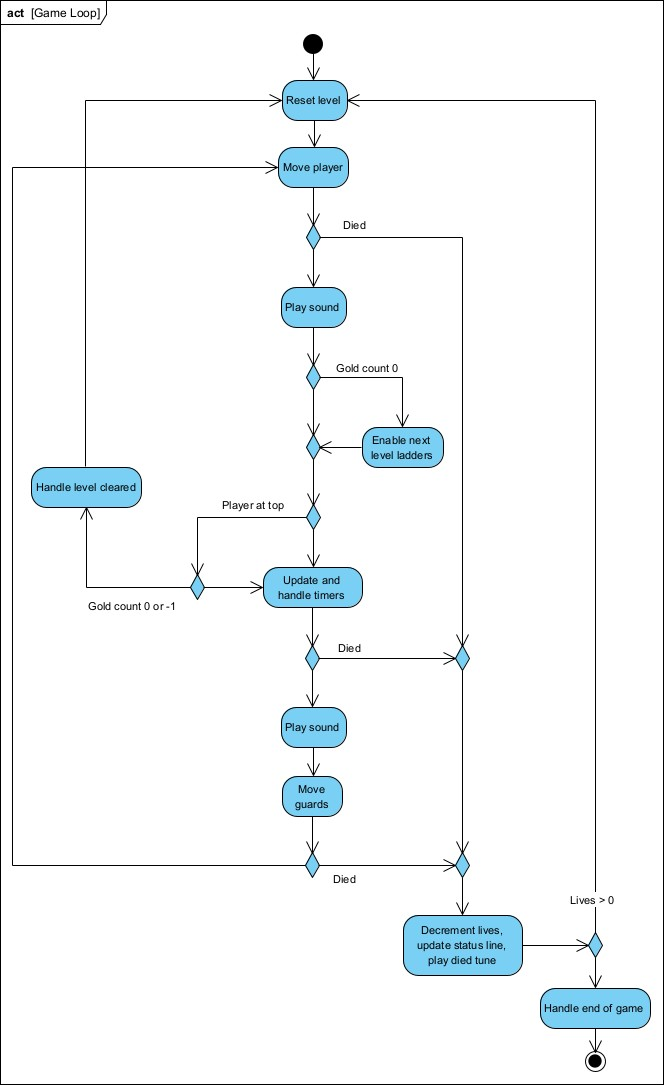
\includegraphics[height=\textheight]{lode_runner_game_loop}
\end{center}

\nwenddocs{}\nwbegincode{550}\sublabel{NW1Xx3lK-4avztR-1}\nwmargintag{{\nwtagstyle{}\subpageref{NW1Xx3lK-4avztR-1}}}\moddef{game loop~{\nwtagstyle{}\subpageref{NW1Xx3lK-4avztR-1}}}\endmoddef\nwstartdeflinemarkup\nwusesondefline{\\{NW1Xx3lK-8jv1b-C}}\nwenddeflinemarkup
    ORG     $609F

.start_game:
    LDX     #$01
    JSR     \nwlinkedidentc{LOAD_LEVEL}{NW1Xx3lK-457nLk-1}
    LDA     #$00
    STA     \nwlinkedidentc{KEY_COMMAND}{NW1Xx3lK-10jlgu-a}
    STA     \nwlinkedidentc{KEY_COMMAND_LR}{NW1Xx3lK-10jlgu-a}
    LDA     \nwlinkedidentc{GAME_MODE}{NW1Xx3lK-10jlgu-S}
    LSR
    ; if \nwlinkedidentc{GAME_MODE}{NW1Xx3lK-10jlgu-S} was 0 or 1 (i.e. not displaying high score screen
    ; or splash screen), play the game.
    BEQ     .play_game

    ; When \nwlinkedidentc{GAME_MODE}{NW1Xx3lK-10jlgu-S} is 2:
    JSR     \nwlinkedidentc{WAIT_KEY}{NW1Xx3lK-31tcsr-1}
    LDA     \nwlinkedidentc{PLAYER_COL}{NW1Xx3lK-10jlgu-M}
    STA     \nwlinkedidentc{GAME_COLNUM}{NW1Xx3lK-10jlgu-7}
    LDA     \nwlinkedidentc{PLAYER_ROW}{NW1Xx3lK-10jlgu-M}
    STA     \nwlinkedidentc{GAME_ROWNUM}{NW1Xx3lK-10jlgu-7}
    LDA     #SPRITE_PLAYER
    JSR     \nwlinkedidentc{WAIT_FOR_KEY_WITH_CURSOR_PAGE_1}{NW1Xx3lK-3Mc2m6-1}

.play_game:
    LDX     #$00
    STX     \nwlinkedidentc{DIG_DIRECTION}{NW1Xx3lK-10jlgu-c}
    STX     \nwlinkedidentc{NOTE_INDEX}{NW1Xx3lK-10jlgu-E}

    LDA     \nwlinkedidentc{GUARD_PATTERN_OFFSET}{NW1Xx3lK-10jlgu-n}
    CLC
    ADC     \nwlinkedidentc{GUARD_COUNT}{NW1Xx3lK-10jlgu-N}         ; \nwlinkedidentc{GUARD_COUNT}{NW1Xx3lK-10jlgu-N} + $97 can't be greater than 8.
    TAY
    LDX     \nwlinkedidentc{TIMES_3_TABLE}{NW1Xx3lK-1W8AJS-U},Y     ; X = 3 * Y (goes up to Y=8)
    LDA     \nwlinkedidentc{GUARD_PATTERNS_LIST}{NW1Xx3lK-1W8AJS-T},X
    STA     \nwlinkedidentc{GUARD_PATTERNS}{NW1Xx3lK-10jlgu-e}
    LDA     \nwlinkedidentc{GUARD_PATTERNS_LIST}{NW1Xx3lK-1W8AJS-T}+1,X
    STA     \nwlinkedidentc{GUARD_PATTERNS}{NW1Xx3lK-10jlgu-e}+1
    LDA     \nwlinkedidentc{GUARD_PATTERNS_LIST}{NW1Xx3lK-1W8AJS-T}+2,X
    STA     \nwlinkedidentc{GUARD_PATTERNS}{NW1Xx3lK-10jlgu-e}+2

    LDY     \nwlinkedidentc{GUARD_PATTERN_OFFSET}{NW1Xx3lK-10jlgu-n}
    LDA     $621D,Y
    STA     \nwlinkedidentc{GUARD_GOLD_TIMER_START_VALUE}{NW1Xx3lK-10jlgu-d}

.game_loop:
    JSR     \nwlinkedidentc{MOVE_PLAYER}{NW1Xx3lK-1viPAs-1}
    LDA     \nwlinkedidentc{ALIVE}{NW1Xx3lK-10jlgu-U}
    BEQ     .died

    JSR     \nwlinkedidentc{PLAY_SOUND}{NW1Xx3lK-4DEk44-1}

    LDA     \nwlinkedidentc{GOLD_COUNT}{NW1Xx3lK-10jlgu-N}
    BNE     .check_player_reached_top
    JSR     \nwlinkedidentc{ENABLE_NEXT_LEVEL_LADDERS}{NW1Xx3lK-on53h-1}

.check_player_reached_top:
    LDA     \nwlinkedidentc{PLAYER_ROW}{NW1Xx3lK-10jlgu-M}
    BNE     .not_at_top
    LDA     \nwlinkedidentc{PLAYER_Y_ADJ}{NW1Xx3lK-10jlgu-P}
    CMP     #$02
    BNE     .not_at_top

    ; Reached top of screen
    LDA     \nwlinkedidentc{GOLD_COUNT}{NW1Xx3lK-10jlgu-N}
    BEQ     .level_cleared
    CMP     #$FF
    BEQ     .level_cleared      ; level cleared if \nwlinkedidentc{GOLD_COUNT}{NW1Xx3lK-10jlgu-N} == 0 or -1.

.not_at_top:
    JSR     \nwlinkedidentc{HANDLE_TIMERS}{NW1Xx3lK-1rQzJG-1}
    LDA     \nwlinkedidentc{ALIVE}{NW1Xx3lK-10jlgu-U}
    BEQ     .died
    JSR     \nwlinkedidentc{PLAY_SOUND}{NW1Xx3lK-4DEk44-1}
    JSR     \nwlinkedidentc{MOVE_GUARDS}{NW1Xx3lK-30nxIi-1}
    LDA     \nwlinkedidentc{ALIVE}{NW1Xx3lK-10jlgu-U}
    BEQ     .died
    BNE     .game_loop

.level_cleared:
    INC     \nwlinkedidentc{LEVELNUM}{NW1Xx3lK-10jlgu-D}
    INC     DISK_LEVEL_LOC
    INC     \nwlinkedidentc{LIVES}{NW1Xx3lK-10jlgu-D}
    BNE     .lives_incremented
    DEC     \nwlinkedidentc{LIVES}{NW1Xx3lK-10jlgu-D}               ; \nwlinkedidentc{LIVES}{NW1Xx3lK-10jlgu-D} doesn't overflow.

.lives_incremented:
    ; Increment score by 1500, playing an ascending tune while doing so.
    LDX     #$0F
    STX     \nwlinkedidentc{SCRATCH_5C}{NW1Xx3lK-10jlgu-1}

.loop2:
    LDY     #$01
    LDA     #$00
    JSR     \nwlinkedidentc{ADD_AND_UPDATE_SCORE}{NW1Xx3lK-J3zE9-1}    ; \nwlinkedidentc{SCORE}{NW1Xx3lK-10jlgu-C} += 100
    JSR     \nwlinkedidentc{APPEND_LEVEL_CLEARED_NOTE}{NW1Xx3lK-IdV4u-1}
    JSR     \nwlinkedidentc{APPEND_LEVEL_CLEARED_NOTE}{NW1Xx3lK-IdV4u-1}
    JSR     \nwlinkedidentc{APPEND_LEVEL_CLEARED_NOTE}{NW1Xx3lK-IdV4u-1}
    DEC     \nwlinkedidentc{SCRATCH_5C}{NW1Xx3lK-10jlgu-1}
    BNE     .loop2

.start_game_:
    JMP     .start_game

.died:
    DEC     \nwlinkedidentc{LIVES}{NW1Xx3lK-10jlgu-D}
    JSR     \nwlinkedidentc{PUT_STATUS_LIVES}{NW1Xx3lK-458dZ9-1}
    JSR     \nwlinkedidentc{LOAD_SOUND_DATA}{NW1Xx3lK-90gdY-1}
    HEX     02 40 02 40 03 50 03 50 04 60 04 60 05 70 05 70
    HEX     06 80 06 80 07 90 07 90 08 A0 08 A0 09 B0 09 B0
    HEX     0A C0 0A C0 0B D0 0B D0 0C E0 0C E0 0D F0 0D F0
    HEX     00

.play_died_tune:
    JSR     \nwlinkedidentc{PLAY_SOUND}{NW1Xx3lK-4DEk44-1}
    BCS     .play_died_tune

    LDA     \nwlinkedidentc{GAME_MODE}{NW1Xx3lK-10jlgu-S}
    LSR
    BEQ     .restore_enable_sound     ; If \nwlinkedidentc{GAME_MODE}{NW1Xx3lK-10jlgu-S} is 0 or 1

    LDA     \nwlinkedidentc{LIVES}{NW1Xx3lK-10jlgu-D}
    BNE     .start_game_    ; We can still play.

    ; Game over
    JSR     \nwlinkedidentc{RECORD_HI_SCORE_DATA_TO_DISK}{NW1Xx3lK-2aVzCP-1}
    JSR     SPINNING_GAME_OVER
    BCS     .key_pressed

\nwused{\\{NW1Xx3lK-8jv1b-C}}\nwidentuses{\\{{\nwixident{ADD{\_}AND{\_}UPDATE{\_}SCORE}}{ADD:unAND:unUPDATE:unSCORE}}\\{{\nwixident{ALIVE}}{ALIVE}}\\{{\nwixident{APPEND{\_}LEVEL{\_}CLEARED{\_}NOTE}}{APPEND:unLEVEL:unCLEARED:unNOTE}}\\{{\nwixident{DIG{\_}DIRECTION}}{DIG:unDIRECTION}}\\{{\nwixident{ENABLE{\_}NEXT{\_}LEVEL{\_}LADDERS}}{ENABLE:unNEXT:unLEVEL:unLADDERS}}\\{{\nwixident{GAME{\_}COLNUM}}{GAME:unCOLNUM}}\\{{\nwixident{GAME{\_}MODE}}{GAME:unMODE}}\\{{\nwixident{GAME{\_}ROWNUM}}{GAME:unROWNUM}}\\{{\nwixident{GOLD{\_}COUNT}}{GOLD:unCOUNT}}\\{{\nwixident{GUARD{\_}COUNT}}{GUARD:unCOUNT}}\\{{\nwixident{GUARD{\_}GOLD{\_}TIMER{\_}START{\_}VALUE}}{GUARD:unGOLD:unTIMER:unSTART:unVALUE}}\\{{\nwixident{GUARD{\_}PATTERN{\_}OFFSET}}{GUARD:unPATTERN:unOFFSET}}\\{{\nwixident{GUARD{\_}PATTERNS}}{GUARD:unPATTERNS}}\\{{\nwixident{GUARD{\_}PATTERNS{\_}LIST}}{GUARD:unPATTERNS:unLIST}}\\{{\nwixident{HANDLE{\_}TIMERS}}{HANDLE:unTIMERS}}\\{{\nwixident{KEY{\_}COMMAND}}{KEY:unCOMMAND}}\\{{\nwixident{KEY{\_}COMMAND{\_}LR}}{KEY:unCOMMAND:unLR}}\\{{\nwixident{LEVELNUM}}{LEVELNUM}}\\{{\nwixident{LIVES}}{LIVES}}\\{{\nwixident{LOAD{\_}LEVEL}}{LOAD:unLEVEL}}\\{{\nwixident{LOAD{\_}SOUND{\_}DATA}}{LOAD:unSOUND:unDATA}}\\{{\nwixident{MOVE{\_}GUARDS}}{MOVE:unGUARDS}}\\{{\nwixident{MOVE{\_}PLAYER}}{MOVE:unPLAYER}}\\{{\nwixident{NOTE{\_}INDEX}}{NOTE:unINDEX}}\\{{\nwixident{PLAY{\_}SOUND}}{PLAY:unSOUND}}\\{{\nwixident{PLAYER{\_}COL}}{PLAYER:unCOL}}\\{{\nwixident{PLAYER{\_}ROW}}{PLAYER:unROW}}\\{{\nwixident{PLAYER{\_}Y{\_}ADJ}}{PLAYER:unY:unADJ}}\\{{\nwixident{PUT{\_}STATUS{\_}LIVES}}{PUT:unSTATUS:unLIVES}}\\{{\nwixident{RECORD{\_}HI{\_}SCORE{\_}DATA{\_}TO{\_}DISK}}{RECORD:unHI:unSCORE:unDATA:unTO:unDISK}}\\{{\nwixident{SCORE}}{SCORE}}\\{{\nwixident{SCRATCH{\_}5C}}{SCRATCH:un5C}}\\{{\nwixident{TIMES{\_}3{\_}TABLE}}{TIMES:un3:unTABLE}}\\{{\nwixident{WAIT{\_}FOR{\_}KEY{\_}WITH{\_}CURSOR{\_}PAGE{\_}1}}{WAIT:unFOR:unKEY:unWITH:unCURSOR:unPAGE:un1}}\\{{\nwixident{WAIT{\_}KEY}}{WAIT:unKEY}}}\nwindexuse{\nwixident{ADD{\_}AND{\_}UPDATE{\_}SCORE}}{ADD:unAND:unUPDATE:unSCORE}{NW1Xx3lK-4avztR-1}\nwindexuse{\nwixident{ALIVE}}{ALIVE}{NW1Xx3lK-4avztR-1}\nwindexuse{\nwixident{APPEND{\_}LEVEL{\_}CLEARED{\_}NOTE}}{APPEND:unLEVEL:unCLEARED:unNOTE}{NW1Xx3lK-4avztR-1}\nwindexuse{\nwixident{DIG{\_}DIRECTION}}{DIG:unDIRECTION}{NW1Xx3lK-4avztR-1}\nwindexuse{\nwixident{ENABLE{\_}NEXT{\_}LEVEL{\_}LADDERS}}{ENABLE:unNEXT:unLEVEL:unLADDERS}{NW1Xx3lK-4avztR-1}\nwindexuse{\nwixident{GAME{\_}COLNUM}}{GAME:unCOLNUM}{NW1Xx3lK-4avztR-1}\nwindexuse{\nwixident{GAME{\_}MODE}}{GAME:unMODE}{NW1Xx3lK-4avztR-1}\nwindexuse{\nwixident{GAME{\_}ROWNUM}}{GAME:unROWNUM}{NW1Xx3lK-4avztR-1}\nwindexuse{\nwixident{GOLD{\_}COUNT}}{GOLD:unCOUNT}{NW1Xx3lK-4avztR-1}\nwindexuse{\nwixident{GUARD{\_}COUNT}}{GUARD:unCOUNT}{NW1Xx3lK-4avztR-1}\nwindexuse{\nwixident{GUARD{\_}GOLD{\_}TIMER{\_}START{\_}VALUE}}{GUARD:unGOLD:unTIMER:unSTART:unVALUE}{NW1Xx3lK-4avztR-1}\nwindexuse{\nwixident{GUARD{\_}PATTERN{\_}OFFSET}}{GUARD:unPATTERN:unOFFSET}{NW1Xx3lK-4avztR-1}\nwindexuse{\nwixident{GUARD{\_}PATTERNS}}{GUARD:unPATTERNS}{NW1Xx3lK-4avztR-1}\nwindexuse{\nwixident{GUARD{\_}PATTERNS{\_}LIST}}{GUARD:unPATTERNS:unLIST}{NW1Xx3lK-4avztR-1}\nwindexuse{\nwixident{HANDLE{\_}TIMERS}}{HANDLE:unTIMERS}{NW1Xx3lK-4avztR-1}\nwindexuse{\nwixident{KEY{\_}COMMAND}}{KEY:unCOMMAND}{NW1Xx3lK-4avztR-1}\nwindexuse{\nwixident{KEY{\_}COMMAND{\_}LR}}{KEY:unCOMMAND:unLR}{NW1Xx3lK-4avztR-1}\nwindexuse{\nwixident{LEVELNUM}}{LEVELNUM}{NW1Xx3lK-4avztR-1}\nwindexuse{\nwixident{LIVES}}{LIVES}{NW1Xx3lK-4avztR-1}\nwindexuse{\nwixident{LOAD{\_}LEVEL}}{LOAD:unLEVEL}{NW1Xx3lK-4avztR-1}\nwindexuse{\nwixident{LOAD{\_}SOUND{\_}DATA}}{LOAD:unSOUND:unDATA}{NW1Xx3lK-4avztR-1}\nwindexuse{\nwixident{MOVE{\_}GUARDS}}{MOVE:unGUARDS}{NW1Xx3lK-4avztR-1}\nwindexuse{\nwixident{MOVE{\_}PLAYER}}{MOVE:unPLAYER}{NW1Xx3lK-4avztR-1}\nwindexuse{\nwixident{NOTE{\_}INDEX}}{NOTE:unINDEX}{NW1Xx3lK-4avztR-1}\nwindexuse{\nwixident{PLAY{\_}SOUND}}{PLAY:unSOUND}{NW1Xx3lK-4avztR-1}\nwindexuse{\nwixident{PLAYER{\_}COL}}{PLAYER:unCOL}{NW1Xx3lK-4avztR-1}\nwindexuse{\nwixident{PLAYER{\_}ROW}}{PLAYER:unROW}{NW1Xx3lK-4avztR-1}\nwindexuse{\nwixident{PLAYER{\_}Y{\_}ADJ}}{PLAYER:unY:unADJ}{NW1Xx3lK-4avztR-1}\nwindexuse{\nwixident{PUT{\_}STATUS{\_}LIVES}}{PUT:unSTATUS:unLIVES}{NW1Xx3lK-4avztR-1}\nwindexuse{\nwixident{RECORD{\_}HI{\_}SCORE{\_}DATA{\_}TO{\_}DISK}}{RECORD:unHI:unSCORE:unDATA:unTO:unDISK}{NW1Xx3lK-4avztR-1}\nwindexuse{\nwixident{SCORE}}{SCORE}{NW1Xx3lK-4avztR-1}\nwindexuse{\nwixident{SCRATCH{\_}5C}}{SCRATCH:un5C}{NW1Xx3lK-4avztR-1}\nwindexuse{\nwixident{TIMES{\_}3{\_}TABLE}}{TIMES:un3:unTABLE}{NW1Xx3lK-4avztR-1}\nwindexuse{\nwixident{WAIT{\_}FOR{\_}KEY{\_}WITH{\_}CURSOR{\_}PAGE{\_}1}}{WAIT:unFOR:unKEY:unWITH:unCURSOR:unPAGE:un1}{NW1Xx3lK-4avztR-1}\nwindexuse{\nwixident{WAIT{\_}KEY}}{WAIT:unKEY}{NW1Xx3lK-4avztR-1}\nwendcode{}\nwbegindocs{551}\nwdocspar

\nwenddocs{}\nwbegincode{552}\sublabel{NW1Xx3lK-1W8AJS-U}\nwmargintag{{\nwtagstyle{}\subpageref{NW1Xx3lK-1W8AJS-U}}}\moddef{tables~{\nwtagstyle{}\subpageref{NW1Xx3lK-1W8AJS-1}}}\plusendmoddef\nwstartdeflinemarkup\nwusesondefline{\\{NW1Xx3lK-1p0Y9w-1}}\nwprevnextdefs{NW1Xx3lK-1W8AJS-T}{NW1Xx3lK-1W8AJS-V}\nwenddeflinemarkup
    ORG     $6214
\nwlinkedidentc{TIMES_3_TABLE}{NW1Xx3lK-1W8AJS-U}:
    HEX     00 03 06 09 0C 0F 12 15 18
\nwindexdefn{\nwixident{TIMES{\_}3{\_}TABLE}}{TIMES:un3:unTABLE}{NW1Xx3lK-1W8AJS-U}\eatline
\nwused{\\{NW1Xx3lK-1p0Y9w-1}}\nwidentdefs{\\{{\nwixident{TIMES{\_}3{\_}TABLE}}{TIMES:un3:unTABLE}}}\nwendcode{}\nwbegindocs{553}\nwdocspar
\nwenddocs{}\nwbegincode{554}\sublabel{NW1Xx3lK-1W8AJS-V}\nwmargintag{{\nwtagstyle{}\subpageref{NW1Xx3lK-1W8AJS-V}}}\moddef{tables~{\nwtagstyle{}\subpageref{NW1Xx3lK-1W8AJS-1}}}\plusendmoddef\nwstartdeflinemarkup\nwusesondefline{\\{NW1Xx3lK-1p0Y9w-1}}\nwprevnextdefs{NW1Xx3lK-1W8AJS-U}{NW1Xx3lK-1W8AJS-W}\nwenddeflinemarkup
    ORG     $8C35
TABLE0:
    HEX     80 80 80 80 80 80 80 80 80 80 80 80 80 80
TABLE1:
    HEX     C0 AA D5 AA D5 AA D5 AA D5 AA D5 AA D5 80
TABLE2:
    HEX     90 80 80 80 80 80 80 80 80 80 80 80 80 82
TABLE3:
    HEX     90 AA D1 A2 D5 A8 85 A8 C5 A2 D4 A2 95 82
TABLE4:
    HEX     90 82 91 A2 C5 A8 80 88 C5 A2 94 A0 90 82
TABLE5:
    HEX     90 82 90 A2 C4 A8 80 88 C5 A2 94 A0 90 82
TABLE6:
    HEX     90 82 90 A2 C4 A8 81 88 C4 A2 D4 A0 95 82
TABLE7:
    HEX     90 A2 D1 A2 C4 88 80 88 C4 A2 84 A0 85 82
TABLE8:
    HEX     90 82 91 A2 C4 88 80 88 C4 AA 84 A0 85 82
TABLE9:
    HEX     90 82 91 A2 C4 88 80 88 C4 8A 84 A0 91 82
TABLE10:
    HEX     90 AA 91 A2 C4 A8 85 A8 85 82 D4 A2 91 82

    ORG     $8CCF
\nwlinkedidentc{ADDRESS_TABLE}{NW1Xx3lK-1W8AJS-V}:
    WORD    TABLE0-13
    WORD    TABLE1-13
    WORD    TABLE2-13
    WORD    TABLE3-13
    WORD    TABLE4-13
    WORD    TABLE5-13
    WORD    TABLE6-13
    WORD    TABLE7-13
    WORD    TABLE8-13
    WORD    TABLE9-13
    WORD    TABLE10-13
\nwindexdefn{\nwixident{ADDRESS{\_}TABLE}}{ADDRESS:unTABLE}{NW1Xx3lK-1W8AJS-V}\eatline
\nwused{\\{NW1Xx3lK-1p0Y9w-1}}\nwidentdefs{\\{{\nwixident{ADDRESS{\_}TABLE}}{ADDRESS:unTABLE}}}\nwendcode{}\nwbegindocs{555}\nwdocspar
\nwenddocs{}\nwbegincode{556}\sublabel{NW1Xx3lK-1avPaD-1}\nwmargintag{{\nwtagstyle{}\subpageref{NW1Xx3lK-1avPaD-1}}}\moddef{anims~{\nwtagstyle{}\subpageref{NW1Xx3lK-1avPaD-1}}}\endmoddef\nwstartdeflinemarkup\nwusesondefline{\\{NW1Xx3lK-8jv1b-C}}\nwenddeflinemarkup
    ORG     $8B1A
SPINNING_GAME_OVER:
    SUBROUTINE

    LDA     #$01
    STA     \nwlinkedidentc{ANIM_COUNT}{NW1Xx3lK-3sWlSS-1}
    LDA     #$20
    STA     \nwlinkedidentc{HGR_PAGE}{NW1Xx3lK-10jlgu-5}

.loop:
    JSR     ANIM5
    JSR     ANIM4
    JSR     ANIM3
    JSR     ANIM2
    JSR     ANIM1
    JSR     ANIM0
    JSR     ANIM1
    JSR     ANIM2
    JSR     ANIM3
    JSR     ANIM4
    JSR     ANIM5
    JSR     ANIM10
    JSR     ANIM9
    JSR     ANIM8
    JSR     ANIM7
    JSR     ANIM6
    JSR     ANIM7
    JSR     ANIM8
    JSR     ANIM9
    JSR     ANIM10
    LDA     \nwlinkedidentc{ANIM_COUNT}{NW1Xx3lK-3sWlSS-1}
    CMP     #100
    BCC     .loop

    JSR     ANIM5
    JSR     ANIM4
    JSR     ANIM3
    JSR     ANIM2
    JSR     ANIM1
    JSR     ANIM0
    CLC
    RTS

    ORG     $8B7A
ANIM0:
    JSR     \nwlinkedidentc{SHOW_ANIM_LINE}{NW1Xx3lK-3sWlSS-1}
    HEX     00 01 02 03 04 05 06 07 08 09 0A 02 01 00
ANIM1:
    JSR     \nwlinkedidentc{SHOW_ANIM_LINE}{NW1Xx3lK-3sWlSS-1}
    HEX     00 00 01 02 03 04 05 07 09 0A 02 01 00 00
ANIM2:
    JSR     \nwlinkedidentc{SHOW_ANIM_LINE}{NW1Xx3lK-3sWlSS-1}
    HEX     00 00 00 01 02 03 04 09 0A 02 01 00 00 00
ANIM3:
    JSR     \nwlinkedidentc{SHOW_ANIM_LINE}{NW1Xx3lK-3sWlSS-1}
    HEX     00 00 00 00 01 02 03 0A 02 01 00 00 00 00
ANIM4:
    JSR     \nwlinkedidentc{SHOW_ANIM_LINE}{NW1Xx3lK-3sWlSS-1}
    HEX     00 00 00 00 00 01 03 0A 01 00 00 00 00 00
ANIM5:
    JSR     \nwlinkedidentc{SHOW_ANIM_LINE}{NW1Xx3lK-3sWlSS-1}
    HEX     00 00 00 00 00 00 01 01 00 00 00 00 00 00
ANIM6:
    JSR     \nwlinkedidentc{SHOW_ANIM_LINE}{NW1Xx3lK-3sWlSS-1}
    HEX     00 01 02 0A 09 08 07 06 05 04 03 02 01 00
ANIM7:
    JSR     \nwlinkedidentc{SHOW_ANIM_LINE}{NW1Xx3lK-3sWlSS-1}
    HEX     00 00 01 02 0A 09 07 05 04 03 02 01 00 00
ANIM8:
    JSR     \nwlinkedidentc{SHOW_ANIM_LINE}{NW1Xx3lK-3sWlSS-1}
    HEX     00 00 00 01 02 0A 09 04 03 02 01 00 00 00
ANIM9:
    JSR     \nwlinkedidentc{SHOW_ANIM_LINE}{NW1Xx3lK-3sWlSS-1}
    HEX     00 00 00 00 01 02 0A 03 02 01 00 00 00 00
ANIM10:
    JSR     \nwlinkedidentc{SHOW_ANIM_LINE}{NW1Xx3lK-3sWlSS-1}
    HEX     00 00 00 00 00 01 0A 03 01 00 00 00 00 00
\nwused{\\{NW1Xx3lK-8jv1b-C}}\nwidentuses{\\{{\nwixident{ANIM{\_}COUNT}}{ANIM:unCOUNT}}\\{{\nwixident{HGR{\_}PAGE}}{HGR:unPAGE}}\\{{\nwixident{SHOW{\_}ANIM{\_}LINE}}{SHOW:unANIM:unLINE}}}\nwindexuse{\nwixident{ANIM{\_}COUNT}}{ANIM:unCOUNT}{NW1Xx3lK-1avPaD-1}\nwindexuse{\nwixident{HGR{\_}PAGE}}{HGR:unPAGE}{NW1Xx3lK-1avPaD-1}\nwindexuse{\nwixident{SHOW{\_}ANIM{\_}LINE}}{SHOW:unANIM:unLINE}{NW1Xx3lK-1avPaD-1}\nwendcode{}\nwbegindocs{557}\nwdocspar

\nwenddocs{}\nwbegincode{558}\sublabel{NW1Xx3lK-3sWlSS-1}\nwmargintag{{\nwtagstyle{}\subpageref{NW1Xx3lK-3sWlSS-1}}}\moddef{show anim line~{\nwtagstyle{}\subpageref{NW1Xx3lK-3sWlSS-1}}}\endmoddef\nwstartdeflinemarkup\nwusesondefline{\\{NW1Xx3lK-8jv1b-C}}\nwenddeflinemarkup
    ORG     $8CE5
\nwlinkedidentc{SHOW_ANIM_LINE}{NW1Xx3lK-3sWlSS-1}:
    SUBROUTINE

    PLA
    STA     \nwlinkedidentc{TMP_PTR}{NW1Xx3lK-10jlgu-1}
    PLA
    STA     \nwlinkedidentc{TMP_PTR}{NW1Xx3lK-10jlgu-1}+1           ; store "return" addr

    ; Fill 14 rows of pixel data from row 0x51 (81) through 0x5E (94).
    LDY     #$50
    STY     \nwlinkedidentc{GAME_ROWNUM}{NW1Xx3lK-10jlgu-7}
    BNE     .next      ; unconditional

.loop:
    JSR     \nwlinkedidentc{ROW_TO_ADDR}{NW1Xx3lK-8jv1b-3}
    LDY     #$00
    LDA     (\nwlinkedidentc{TMP_PTR}{NW1Xx3lK-10jlgu-1}),Y
    ASL
    TAX
    LDA     \nwlinkedidentc{ADDRESS_TABLE}{NW1Xx3lK-1W8AJS-V},X
    STA     .loop2+1
    LDA     \nwlinkedidentc{ADDRESS_TABLE}{NW1Xx3lK-1W8AJS-V}+1,X   ; groups of 14 bytes
    STA     .loop2+2
    LDY     #$0D

    ; Copy 13 bytes of pixel data onto screen from
    ; addr+14 to addr+26
.loop2:
    LDA     $8D08,Y             ; fixed up from above
    STA     (\nwlinkedidentc{ROW_ADDR}{NW1Xx3lK-10jlgu-5}),Y        ; pixel data
    INY
    CPY     #$1B
    BCC     .loop2              ; Y < 27

    ; Next row
.next:
    JSR     \nwlinkedidentc{INCREMENT_TMP_PTR}{NW1Xx3lK-3sWlSS-1}
    INC     \nwlinkedidentc{GAME_ROWNUM}{NW1Xx3lK-10jlgu-7}
    LDY     \nwlinkedidentc{GAME_ROWNUM}{NW1Xx3lK-10jlgu-7}
    CPY     #$5F
    BCC     .loop

    LDX     \nwlinkedidentc{ANIM_COUNT}{NW1Xx3lK-3sWlSS-1}
    LDY     #$FF
.delay:
    DEY
    BNE     .delay
    DEX
    BNE     .delay
    INC     \nwlinkedidentc{ANIM_COUNT}{NW1Xx3lK-3sWlSS-1}

    LDA     \nwlinkedidentc{INPUT_MODE}{NW1Xx3lK-10jlgu-I}
    CMP     #KEYBOARD_MODE
    BEQ     .check_for_keypress
    LDA     \nwlinkedidentc{BUTN1}{NW1Xx3lK-10jlgu-I}
    BMI     .input_detected
    LDA     \nwlinkedidentc{BUTN0}{NW1Xx3lK-10jlgu-I}
    BMI     .input_detected

.check_for_keypress:
    LDA     \nwlinkedidentc{KBD}{NW1Xx3lK-10jlgu-J}
    BMI     .input_detected
    RTS

    ; Skip the rest of the big animation.
.input_detected:
    PLA
    PLA
    SEC
    LDA     \nwlinkedidentc{KBD}{NW1Xx3lK-10jlgu-J}
    STA     \nwlinkedidentc{KBDSTRB}{NW1Xx3lK-10jlgu-J}
    RTS

    ORG     $8D4B
\nwlinkedidentc{ANIM_COUNT}{NW1Xx3lK-3sWlSS-1}:
    HEX     9D

    ORG     $8D4C
\nwlinkedidentc{INCREMENT_TMP_PTR}{NW1Xx3lK-3sWlSS-1}:
    SUBROUTINE

    INC     \nwlinkedidentc{TMP_PTR}{NW1Xx3lK-10jlgu-1}
    BNE     .end
    INC     \nwlinkedidentc{TMP_PTR}{NW1Xx3lK-10jlgu-1}+1
.end:
    RTS
\nwindexdefn{\nwixident{SHOW{\_}ANIM{\_}LINE}}{SHOW:unANIM:unLINE}{NW1Xx3lK-3sWlSS-1}\nwindexdefn{\nwixident{ANIM{\_}COUNT}}{ANIM:unCOUNT}{NW1Xx3lK-3sWlSS-1}\nwindexdefn{\nwixident{INCREMENT{\_}TMP{\_}PTR}}{INCREMENT:unTMP:unPTR}{NW1Xx3lK-3sWlSS-1}\eatline
\nwused{\\{NW1Xx3lK-8jv1b-C}}\nwidentdefs{\\{{\nwixident{ANIM{\_}COUNT}}{ANIM:unCOUNT}}\\{{\nwixident{INCREMENT{\_}TMP{\_}PTR}}{INCREMENT:unTMP:unPTR}}\\{{\nwixident{SHOW{\_}ANIM{\_}LINE}}{SHOW:unANIM:unLINE}}}\nwidentuses{\\{{\nwixident{ADDRESS{\_}TABLE}}{ADDRESS:unTABLE}}\\{{\nwixident{BUTN0}}{BUTN0}}\\{{\nwixident{BUTN1}}{BUTN1}}\\{{\nwixident{GAME{\_}ROWNUM}}{GAME:unROWNUM}}\\{{\nwixident{INPUT{\_}MODE}}{INPUT:unMODE}}\\{{\nwixident{KBD}}{KBD}}\\{{\nwixident{KBDSTRB}}{KBDSTRB}}\\{{\nwixident{ROW{\_}ADDR}}{ROW:unADDR}}\\{{\nwixident{ROW{\_}TO{\_}ADDR}}{ROW:unTO:unADDR}}\\{{\nwixident{TMP{\_}PTR}}{TMP:unPTR}}}\nwindexuse{\nwixident{ADDRESS{\_}TABLE}}{ADDRESS:unTABLE}{NW1Xx3lK-3sWlSS-1}\nwindexuse{\nwixident{BUTN0}}{BUTN0}{NW1Xx3lK-3sWlSS-1}\nwindexuse{\nwixident{BUTN1}}{BUTN1}{NW1Xx3lK-3sWlSS-1}\nwindexuse{\nwixident{GAME{\_}ROWNUM}}{GAME:unROWNUM}{NW1Xx3lK-3sWlSS-1}\nwindexuse{\nwixident{INPUT{\_}MODE}}{INPUT:unMODE}{NW1Xx3lK-3sWlSS-1}\nwindexuse{\nwixident{KBD}}{KBD}{NW1Xx3lK-3sWlSS-1}\nwindexuse{\nwixident{KBDSTRB}}{KBDSTRB}{NW1Xx3lK-3sWlSS-1}\nwindexuse{\nwixident{ROW{\_}ADDR}}{ROW:unADDR}{NW1Xx3lK-3sWlSS-1}\nwindexuse{\nwixident{ROW{\_}TO{\_}ADDR}}{ROW:unTO:unADDR}{NW1Xx3lK-3sWlSS-1}\nwindexuse{\nwixident{TMP{\_}PTR}}{TMP:unPTR}{NW1Xx3lK-3sWlSS-1}\nwendcode{}\nwbegindocs{559}\nwdocspar
\chapter{Level editor}

\nwenddocs{}\nwbegincode{560}\sublabel{NW1Xx3lK-1W8AJS-W}\nwmargintag{{\nwtagstyle{}\subpageref{NW1Xx3lK-1W8AJS-W}}}\moddef{tables~{\nwtagstyle{}\subpageref{NW1Xx3lK-1W8AJS-1}}}\plusendmoddef\nwstartdeflinemarkup\nwusesondefline{\\{NW1Xx3lK-1p0Y9w-1}}\nwprevnextdefs{NW1Xx3lK-1W8AJS-V}{NW1Xx3lK-1W8AJS-X}\nwenddeflinemarkup
    ORG     $7C4D
\nwlinkedidentc{EDITOR_KEYS}{NW1Xx3lK-1W8AJS-W}:
    ; P (Play level)
    ; C (Clear level)
    ; E (Edit level)
    ; M (Move level)
    ; I (Initialize disk)
    ; S (clear high Scores)
    HEX     D0 C3 C5 CD C9 D3 00    ; P C E M I S
\nwlinkedidentc{EDITOR_ROUTINE_ADDRESS}{NW1Xx3lK-1W8AJS-W}:
    WORD    \nwlinkedidentc{EDITOR_PLAY_LEVEL}{NW1Xx3lK-4Pn5Im-1}-1
    WORD    \nwlinkedidentc{EDITOR_CLEAR_LEVEL}{NW1Xx3lK-BLWHg-1}-1
    WORD    \nwlinkedidentc{EDITOR_EDIT_LEVEL}{NW1Xx3lK-2M74x9-1}-1
    WORD    \nwlinkedidentc{EDITOR_MOVE_LEVEL}{NW1Xx3lK-23uALT-1}-1
    WORD    \nwlinkedidentc{EDITOR_INITIALIZE_DISK}{NW1Xx3lK-3DVjQa-1}-1
    WORD    EDITOR_CLEAR_HIGH_SCORES-1
\nwindexdefn{\nwixident{EDITOR{\_}KEYS}}{EDITOR:unKEYS}{NW1Xx3lK-1W8AJS-W}\nwindexdefn{\nwixident{EDITOR{\_}ROUTINE{\_}ADDRESS}}{EDITOR:unROUTINE:unADDRESS}{NW1Xx3lK-1W8AJS-W}\eatline
\nwused{\\{NW1Xx3lK-1p0Y9w-1}}\nwidentdefs{\\{{\nwixident{EDITOR{\_}KEYS}}{EDITOR:unKEYS}}\\{{\nwixident{EDITOR{\_}ROUTINE{\_}ADDRESS}}{EDITOR:unROUTINE:unADDRESS}}}\nwidentuses{\\{{\nwixident{EDITOR{\_}CLEAR{\_}LEVEL}}{EDITOR:unCLEAR:unLEVEL}}\\{{\nwixident{EDITOR{\_}EDIT{\_}LEVEL}}{EDITOR:unEDIT:unLEVEL}}\\{{\nwixident{EDITOR{\_}INITIALIZE{\_}DISK}}{EDITOR:unINITIALIZE:unDISK}}\\{{\nwixident{EDITOR{\_}MOVE{\_}LEVEL}}{EDITOR:unMOVE:unLEVEL}}\\{{\nwixident{EDITOR{\_}PLAY{\_}LEVEL}}{EDITOR:unPLAY:unLEVEL}}}\nwindexuse{\nwixident{EDITOR{\_}CLEAR{\_}LEVEL}}{EDITOR:unCLEAR:unLEVEL}{NW1Xx3lK-1W8AJS-W}\nwindexuse{\nwixident{EDITOR{\_}EDIT{\_}LEVEL}}{EDITOR:unEDIT:unLEVEL}{NW1Xx3lK-1W8AJS-W}\nwindexuse{\nwixident{EDITOR{\_}INITIALIZE{\_}DISK}}{EDITOR:unINITIALIZE:unDISK}{NW1Xx3lK-1W8AJS-W}\nwindexuse{\nwixident{EDITOR{\_}MOVE{\_}LEVEL}}{EDITOR:unMOVE:unLEVEL}{NW1Xx3lK-1W8AJS-W}\nwindexuse{\nwixident{EDITOR{\_}PLAY{\_}LEVEL}}{EDITOR:unPLAY:unLEVEL}{NW1Xx3lK-1W8AJS-W}\nwendcode{}\nwbegindocs{561}\nwdocspar
\nwenddocs{}\nwbegincode{562}\sublabel{NW1Xx3lK-2RTwFX-1}\nwmargintag{{\nwtagstyle{}\subpageref{NW1Xx3lK-2RTwFX-1}}}\moddef{level editor~{\nwtagstyle{}\subpageref{NW1Xx3lK-2RTwFX-1}}}\endmoddef\nwstartdeflinemarkup\nwusesondefline{\\{NW1Xx3lK-8jv1b-C}}\nwenddeflinemarkup
    ORG     $7B84
\nwlinkedidentc{LEVEL_EDITOR}{NW1Xx3lK-2RTwFX-1}:
    SUBROUTINE

    LDA     #$00
    STA     \nwlinkedidentc{SCORE}{NW1Xx3lK-10jlgu-C}
    STA     \nwlinkedidentc{SCORE}{NW1Xx3lK-10jlgu-C}+1
    STA     \nwlinkedidentc{SCORE}{NW1Xx3lK-10jlgu-C}+2
    STA     \nwlinkedidentc{SCORE}{NW1Xx3lK-10jlgu-C}+3

    LDA     \nwlinkedidentc{INDIRECT_TARGET}{NW1Xx3lK-3KoKxI-1}
    STA     RWTS_ADDR
    LDA     \nwlinkedidentc{INDIRECT_TARGET}{NW1Xx3lK-3KoKxI-1}+1
    STA     RWTS_ADDR+1

    LDA     #$05
    STA     \nwlinkedidentc{LIVES}{NW1Xx3lK-10jlgu-D}
    STA     \nwlinkedidentc{GAME_MODE}{NW1Xx3lK-10jlgu-S}
    LDA     \nwlinkedidentc{INPUT_MODE}{NW1Xx3lK-10jlgu-I}
    STA     READ_SAVED_INPUT_MODE+1

    LDA     #KEYBOARD_MODE
    STA     \nwlinkedidentc{INPUT_MODE}{NW1Xx3lK-10jlgu-I}

    STA     \nwlinkedidentc{TXTPAGE1}{NW1Xx3lK-10jlgu-Y}

    LDA     DISK_LEVEL_LOC
    CMP     #$96
    BCC     \nwlinkedidentc{START_LEVEL_EDITOR}{NW1Xx3lK-2RTwFX-1}
    LDA     #$00
    STA     DISK_LEVEL_LOC

\nwlinkedidentc{START_LEVEL_EDITOR}{NW1Xx3lK-2RTwFX-1}:
    JSR     \nwlinkedidentc{CLEAR_HGR1}{NW1Xx3lK-8jv1b-1}
    LDA     #$20
    STA     \nwlinkedidentc{DRAW_PAGE}{NW1Xx3lK-10jlgu-9}
    LDA     #$00
    STA     \nwlinkedidentc{GAME_COLNUM}{NW1Xx3lK-10jlgu-7}
    STA     \nwlinkedidentc{GAME_ROWNUM}{NW1Xx3lK-10jlgu-7}

    ; "  LODE RUNNER BOARD EDITOR\\r
    ; "----------------------------\\r
    ; "  <ESC> ABORTS ANY COMMAND\\r"
    JSR     \nwlinkedidentc{PUT_STRING}{NW1Xx3lK-47YPHz-1}
    HEX     A0 A0 CC CF C4 C5 A0 D2 D5 CE CE C5 D2 A0 C2 CF
    HEX     C1 D2 C4 A0 C5 C4 C9 D4 CF D2 8D AD AD AD AD AD
    HEX     AD AD AD AD AD AD AD AD AD AD AD AD AD AD AD AD
    HEX     AD AD AD AD AD AD AD 8D A0 A0 BC C5 D3 C3 BE A0
    HEX     C1 C2 CF D2 D4 D3 A0 C1 CE D9 A0 C3 CF CD CD C1
    HEX     CE C4 8D 00

\nwlinkedidentc{EDITOR_COMMAND_LOOP}{NW1Xx3lK-2RTwFX-1}:
    LDA     \nwlinkedidentc{GAME_ROWNUM}{NW1Xx3lK-10jlgu-7}
    CMP     #$09
    BCS     \nwlinkedidentc{START_LEVEL_EDITOR}{NW1Xx3lK-2RTwFX-1}

    ; "\\r"
    ; "COMMAND>"
    JSR     \nwlinkedidentc{PUT_STRING}{NW1Xx3lK-47YPHz-1}
    HEX     8D C3 CF CD CD C1 CE C4 BE 00

    JSR     \nwlinkedidentc{EDITOR_WAIT_FOR_KEY}{NW1Xx3lK-3khrAL-1}
    LDX     #$00

.loop2:
    LDY     \nwlinkedidentc{EDITOR_KEYS}{NW1Xx3lK-1W8AJS-W},X
    BEQ     EDITOR_COMMAND_LOOP_BEEP
    CMP     \nwlinkedidentc{EDITOR_KEYS}{NW1Xx3lK-1W8AJS-W},X
    BEQ     .end
    INX
    BNE     .loop2

EDITOR_COMMAND_LOOP_BEEP:
    JSR     \nwlinkedidentc{BEEP}{NW1Xx3lK-dU9NC-1}
    JMP     \nwlinkedidentc{EDITOR_COMMAND_LOOP}{NW1Xx3lK-2RTwFX-1}

.end:
    TXA
    ASL
    TAX
    LDA     \nwlinkedidentc{EDITOR_ROUTINE_ADDRESS}{NW1Xx3lK-1W8AJS-W}+1,X
    PHA
    LDA     \nwlinkedidentc{EDITOR_ROUTINE_ADDRESS}{NW1Xx3lK-1W8AJS-W},X
    PHA
    RTS

\nwindexdefn{\nwixident{LEVEL{\_}EDITOR}}{LEVEL:unEDITOR}{NW1Xx3lK-2RTwFX-1}\nwindexdefn{\nwixident{START{\_}LEVEL{\_}EDITOR}}{START:unLEVEL:unEDITOR}{NW1Xx3lK-2RTwFX-1}\nwindexdefn{\nwixident{EDITOR{\_}COMMAND{\_}LOOP}}{EDITOR:unCOMMAND:unLOOP}{NW1Xx3lK-2RTwFX-1}\eatline
\nwused{\\{NW1Xx3lK-8jv1b-C}}\nwidentdefs{\\{{\nwixident{EDITOR{\_}COMMAND{\_}LOOP}}{EDITOR:unCOMMAND:unLOOP}}\\{{\nwixident{LEVEL{\_}EDITOR}}{LEVEL:unEDITOR}}\\{{\nwixident{START{\_}LEVEL{\_}EDITOR}}{START:unLEVEL:unEDITOR}}}\nwidentuses{\\{{\nwixident{BEEP}}{BEEP}}\\{{\nwixident{CLEAR{\_}HGR1}}{CLEAR:unHGR1}}\\{{\nwixident{DRAW{\_}PAGE}}{DRAW:unPAGE}}\\{{\nwixident{EDITOR{\_}KEYS}}{EDITOR:unKEYS}}\\{{\nwixident{EDITOR{\_}ROUTINE{\_}ADDRESS}}{EDITOR:unROUTINE:unADDRESS}}\\{{\nwixident{EDITOR{\_}WAIT{\_}FOR{\_}KEY}}{EDITOR:unWAIT:unFOR:unKEY}}\\{{\nwixident{GAME{\_}COLNUM}}{GAME:unCOLNUM}}\\{{\nwixident{GAME{\_}MODE}}{GAME:unMODE}}\\{{\nwixident{GAME{\_}ROWNUM}}{GAME:unROWNUM}}\\{{\nwixident{INDIRECT{\_}TARGET}}{INDIRECT:unTARGET}}\\{{\nwixident{INPUT{\_}MODE}}{INPUT:unMODE}}\\{{\nwixident{LIVES}}{LIVES}}\\{{\nwixident{PUT{\_}STRING}}{PUT:unSTRING}}\\{{\nwixident{SCORE}}{SCORE}}\\{{\nwixident{TXTPAGE1}}{TXTPAGE1}}}\nwindexuse{\nwixident{BEEP}}{BEEP}{NW1Xx3lK-2RTwFX-1}\nwindexuse{\nwixident{CLEAR{\_}HGR1}}{CLEAR:unHGR1}{NW1Xx3lK-2RTwFX-1}\nwindexuse{\nwixident{DRAW{\_}PAGE}}{DRAW:unPAGE}{NW1Xx3lK-2RTwFX-1}\nwindexuse{\nwixident{EDITOR{\_}KEYS}}{EDITOR:unKEYS}{NW1Xx3lK-2RTwFX-1}\nwindexuse{\nwixident{EDITOR{\_}ROUTINE{\_}ADDRESS}}{EDITOR:unROUTINE:unADDRESS}{NW1Xx3lK-2RTwFX-1}\nwindexuse{\nwixident{EDITOR{\_}WAIT{\_}FOR{\_}KEY}}{EDITOR:unWAIT:unFOR:unKEY}{NW1Xx3lK-2RTwFX-1}\nwindexuse{\nwixident{GAME{\_}COLNUM}}{GAME:unCOLNUM}{NW1Xx3lK-2RTwFX-1}\nwindexuse{\nwixident{GAME{\_}MODE}}{GAME:unMODE}{NW1Xx3lK-2RTwFX-1}\nwindexuse{\nwixident{GAME{\_}ROWNUM}}{GAME:unROWNUM}{NW1Xx3lK-2RTwFX-1}\nwindexuse{\nwixident{INDIRECT{\_}TARGET}}{INDIRECT:unTARGET}{NW1Xx3lK-2RTwFX-1}\nwindexuse{\nwixident{INPUT{\_}MODE}}{INPUT:unMODE}{NW1Xx3lK-2RTwFX-1}\nwindexuse{\nwixident{LIVES}}{LIVES}{NW1Xx3lK-2RTwFX-1}\nwindexuse{\nwixident{PUT{\_}STRING}}{PUT:unSTRING}{NW1Xx3lK-2RTwFX-1}\nwindexuse{\nwixident{SCORE}}{SCORE}{NW1Xx3lK-2RTwFX-1}\nwindexuse{\nwixident{TXTPAGE1}}{TXTPAGE1}{NW1Xx3lK-2RTwFX-1}\nwendcode{}\nwbegindocs{563}\nwdocspar
Clearing a level involves getting the target level number from the user,
waiting for the user to insert a valid data disk, and then writing zeros
to the target level on disk.

\nwenddocs{}\nwbegincode{564}\sublabel{NW1Xx3lK-BLWHg-1}\nwmargintag{{\nwtagstyle{}\subpageref{NW1Xx3lK-BLWHg-1}}}\moddef{editor clear level~{\nwtagstyle{}\subpageref{NW1Xx3lK-BLWHg-1}}}\endmoddef\nwstartdeflinemarkup\nwusesondefline{\\{NW1Xx3lK-8jv1b-C}}\nwenddeflinemarkup
    ORG     $7C8E
\nwlinkedidentc{EDITOR_CLEAR_LEVEL}{NW1Xx3lK-BLWHg-1}:
    SUBROUTINE

    ; "\\r"
    ; ">>CLEAR LEVEL"
    JSR     \nwlinkedidentc{PUT_STRING}{NW1Xx3lK-47YPHz-1}
    HEX     8D BE BE C3 CC C5 C1 D2 A0 CC C5 D6 C5 CC 00

    JSR     \nwlinkedidentc{GET_LEVEL_FROM_KEYBOARD}{NW1Xx3lK-qSm4f-1}
    BCS     .beep
    JSR     \nwlinkedidentc{CHECK_FOR_VALID_DATA_DISK}{NW1Xx3lK-VRsjB-1}

    LDY     #$00
    TYA
.loop:
    STA     DISK_BUFFER,Y
    INY
    BNE     .loop

    LDA     #DISK_ACCESS_WRITE
    JSR     ACCESS_COMPRESSED_LEVEL_DATA      ; write level
    JMP     \nwlinkedidentc{EDITOR_COMMAND_LOOP}{NW1Xx3lK-2RTwFX-1}

.beep:
    JMP     EDITOR_COMMAND_LOOP_BEEP
\nwindexdefn{\nwixident{EDITOR{\_}CLEAR{\_}LEVEL}}{EDITOR:unCLEAR:unLEVEL}{NW1Xx3lK-BLWHg-1}\eatline
\nwused{\\{NW1Xx3lK-8jv1b-C}}\nwidentdefs{\\{{\nwixident{EDITOR{\_}CLEAR{\_}LEVEL}}{EDITOR:unCLEAR:unLEVEL}}}\nwidentuses{\\{{\nwixident{CHECK{\_}FOR{\_}VALID{\_}DATA{\_}DISK}}{CHECK:unFOR:unVALID:unDATA:unDISK}}\\{{\nwixident{EDITOR{\_}COMMAND{\_}LOOP}}{EDITOR:unCOMMAND:unLOOP}}\\{{\nwixident{GET{\_}LEVEL{\_}FROM{\_}KEYBOARD}}{GET:unLEVEL:unFROM:unKEYBOARD}}\\{{\nwixident{PUT{\_}STRING}}{PUT:unSTRING}}}\nwindexuse{\nwixident{CHECK{\_}FOR{\_}VALID{\_}DATA{\_}DISK}}{CHECK:unFOR:unVALID:unDATA:unDISK}{NW1Xx3lK-BLWHg-1}\nwindexuse{\nwixident{EDITOR{\_}COMMAND{\_}LOOP}}{EDITOR:unCOMMAND:unLOOP}{NW1Xx3lK-BLWHg-1}\nwindexuse{\nwixident{GET{\_}LEVEL{\_}FROM{\_}KEYBOARD}}{GET:unLEVEL:unFROM:unKEYBOARD}{NW1Xx3lK-BLWHg-1}\nwindexuse{\nwixident{PUT{\_}STRING}}{PUT:unSTRING}{NW1Xx3lK-BLWHg-1}\nwendcode{}\nwbegindocs{565}\nwdocspar
Moving a level involves getting the source and target level numbers from the user,
waiting for the user to insert the source data disk, reading the source level, waiting
for the user to insert the target data disk, and then writing the current
level data to the target level on disk.

\nwenddocs{}\nwbegincode{566}\sublabel{NW1Xx3lK-10jlgu-o}\nwmargintag{{\nwtagstyle{}\subpageref{NW1Xx3lK-10jlgu-o}}}\moddef{defines~{\nwtagstyle{}\subpageref{NW1Xx3lK-10jlgu-1}}}\plusendmoddef\nwstartdeflinemarkup\nwusesondefline{\\{NW1Xx3lK-1p0Y9w-1}}\nwprevnextdefs{NW1Xx3lK-10jlgu-n}{NW1Xx3lK-10jlgu-p}\nwenddeflinemarkup
    ORG     $824F
\nwlinkedidentc{EDITOR_LEVEL_ENTRY}{NW1Xx3lK-10jlgu-o}:
    HEX     0F
\nwindexdefn{\nwixident{EDITOR{\_}LEVEL{\_}ENTRY}}{EDITOR:unLEVEL:unENTRY}{NW1Xx3lK-10jlgu-o}\eatline
\nwused{\\{NW1Xx3lK-1p0Y9w-1}}\nwidentdefs{\\{{\nwixident{EDITOR{\_}LEVEL{\_}ENTRY}}{EDITOR:unLEVEL:unENTRY}}}\nwendcode{}\nwbegindocs{567}\nwdocspar
\nwenddocs{}\nwbegincode{568}\sublabel{NW1Xx3lK-23uALT-1}\nwmargintag{{\nwtagstyle{}\subpageref{NW1Xx3lK-23uALT-1}}}\moddef{editor move level~{\nwtagstyle{}\subpageref{NW1Xx3lK-23uALT-1}}}\endmoddef\nwstartdeflinemarkup\nwusesondefline{\\{NW1Xx3lK-8jv1b-C}}\nwenddeflinemarkup
    ORG     $7CD8
\nwlinkedidentc{EDITOR_MOVE_LEVEL}{NW1Xx3lK-23uALT-1}:
    SUBROUTINE

    ; "\\r"
    ; ">>MOVE LEVEL"
    JSR     \nwlinkedidentc{PUT_STRING}{NW1Xx3lK-47YPHz-1}
    HEX     8D BE BE CD CF D6 C5 A0 CC C5 D6 C5 CC 00

    JSR     \nwlinkedidentc{GET_LEVEL_FROM_KEYBOARD}{NW1Xx3lK-qSm4f-1}
    BCS     .beep
    STY     \nwlinkedidentc{EDITOR_LEVEL_ENTRY}{NW1Xx3lK-10jlgu-o}      ; source level

    ; " TO LEVEL"
    JSR     \nwlinkedidentc{PUT_STRING}{NW1Xx3lK-47YPHz-1}
    HEX     A0 D4 CF A0 CC C5 D6 C5 CC 00

    JSR     \nwlinkedidentc{GET_LEVEL_FROM_KEYBOARD}{NW1Xx3lK-qSm4f-1}
    BCS     .beep
    STY     \nwlinkedidentc{SAVED_VTOC_DATA}{NW1Xx3lK-1W8AJS-S}         ; convenient place for target level

    ; "\\r"
    ; "  SOURCE DISKETTE"
    JSR     \nwlinkedidentc{PUT_STRING}{NW1Xx3lK-47YPHz-1}
    HEX     8D A0 A0 D3 CF D5 D2 C3 C5 A0 C4 C9 D3 CB C5 D4 D4 C5 00
 
    JSR     \nwlinkedidentc{EDITOR_WAIT_FOR_KEY}{NW1Xx3lK-3khrAL-1}
    ; Deny and dump user back to editor if not valid data disk
    JSR     \nwlinkedidentc{CHECK_FOR_VALID_DATA_DISK}{NW1Xx3lK-VRsjB-1}
    LDA     \nwlinkedidentc{EDITOR_LEVEL_ENTRY}{NW1Xx3lK-10jlgu-o}              ; source level
    STA     DISK_LEVEL_LOC
    LDA     #DISK_ACCESS_READ
    JSR     ACCESS_COMPRESSED_LEVEL_DATA      ; read source level

    ; "\\r"
    ; "  DESTINATION DISKETTE"
    JSR     \nwlinkedidentc{PUT_STRING}{NW1Xx3lK-47YPHz-1}
    HEX     8D A0 A0 C4 C5 D3 D4 C9 CE C1 D4 C9 CF CE A0 C4 C9 D3 CB C5 D4 D4 C5 00

    JSR     \nwlinkedidentc{EDITOR_WAIT_FOR_KEY}{NW1Xx3lK-3khrAL-1}
    ; Deny and dump user back to editor if not valid data disk
    JSR     \nwlinkedidentc{CHECK_FOR_VALID_DATA_DISK}{NW1Xx3lK-VRsjB-1}
    LDA     \nwlinkedidentc{SAVED_VTOC_DATA}{NW1Xx3lK-1W8AJS-S}                 ; target level
    STA     DISK_LEVEL_LOC
    LDA     #DISK_ACCESS_WRITE
    JSR     ACCESS_COMPRESSED_LEVEL_DATA      ; write target level
    JMP     \nwlinkedidentc{EDITOR_COMMAND_LOOP}{NW1Xx3lK-2RTwFX-1}

.beep:
    JMP     EDITOR_COMMAND_LOOP_BEEP
\nwindexdefn{\nwixident{EDITOR{\_}MOVE{\_}LEVEL}}{EDITOR:unMOVE:unLEVEL}{NW1Xx3lK-23uALT-1}\eatline
\nwused{\\{NW1Xx3lK-8jv1b-C}}\nwidentdefs{\\{{\nwixident{EDITOR{\_}MOVE{\_}LEVEL}}{EDITOR:unMOVE:unLEVEL}}}\nwidentuses{\\{{\nwixident{CHECK{\_}FOR{\_}VALID{\_}DATA{\_}DISK}}{CHECK:unFOR:unVALID:unDATA:unDISK}}\\{{\nwixident{EDITOR{\_}COMMAND{\_}LOOP}}{EDITOR:unCOMMAND:unLOOP}}\\{{\nwixident{EDITOR{\_}LEVEL{\_}ENTRY}}{EDITOR:unLEVEL:unENTRY}}\\{{\nwixident{EDITOR{\_}WAIT{\_}FOR{\_}KEY}}{EDITOR:unWAIT:unFOR:unKEY}}\\{{\nwixident{GET{\_}LEVEL{\_}FROM{\_}KEYBOARD}}{GET:unLEVEL:unFROM:unKEYBOARD}}\\{{\nwixident{PUT{\_}STRING}}{PUT:unSTRING}}\\{{\nwixident{SAVED{\_}VTOC{\_}DATA}}{SAVED:unVTOC:unDATA}}}\nwindexuse{\nwixident{CHECK{\_}FOR{\_}VALID{\_}DATA{\_}DISK}}{CHECK:unFOR:unVALID:unDATA:unDISK}{NW1Xx3lK-23uALT-1}\nwindexuse{\nwixident{EDITOR{\_}COMMAND{\_}LOOP}}{EDITOR:unCOMMAND:unLOOP}{NW1Xx3lK-23uALT-1}\nwindexuse{\nwixident{EDITOR{\_}LEVEL{\_}ENTRY}}{EDITOR:unLEVEL:unENTRY}{NW1Xx3lK-23uALT-1}\nwindexuse{\nwixident{EDITOR{\_}WAIT{\_}FOR{\_}KEY}}{EDITOR:unWAIT:unFOR:unKEY}{NW1Xx3lK-23uALT-1}\nwindexuse{\nwixident{GET{\_}LEVEL{\_}FROM{\_}KEYBOARD}}{GET:unLEVEL:unFROM:unKEYBOARD}{NW1Xx3lK-23uALT-1}\nwindexuse{\nwixident{PUT{\_}STRING}}{PUT:unSTRING}{NW1Xx3lK-23uALT-1}\nwindexuse{\nwixident{SAVED{\_}VTOC{\_}DATA}}{SAVED:unVTOC:unDATA}{NW1Xx3lK-23uALT-1}\nwendcode{}\nwbegindocs{569}\nwdocspar
\nwenddocs{}\nwbegincode{570}\sublabel{NW1Xx3lK-4Pn5Im-1}\nwmargintag{{\nwtagstyle{}\subpageref{NW1Xx3lK-4Pn5Im-1}}}\moddef{editor play level~{\nwtagstyle{}\subpageref{NW1Xx3lK-4Pn5Im-1}}}\endmoddef\nwstartdeflinemarkup\nwusesondefline{\\{NW1Xx3lK-8jv1b-C}}\nwenddeflinemarkup
    ORG     $7C60
\nwlinkedidentc{EDITOR_PLAY_LEVEL}{NW1Xx3lK-4Pn5Im-1}:
    SUBROUTINE

    ; "\\r"
    ; ">>PLAY LEVEL"
    JSR     \nwlinkedidentc{PUT_STRING}{NW1Xx3lK-47YPHz-1}
    HEX     8D BE BE D0 CC C1 D9 A0 CC C5 D6 C5 CC 00

    JSR     \nwlinkedidentc{GET_LEVEL_FROM_KEYBOARD}{NW1Xx3lK-qSm4f-1}
    BCS     .beep

READ_SAVED_INPUT_MODE:
    LDA     #$00
    STA     \nwlinkedidentc{INPUT_MODE}{NW1Xx3lK-10jlgu-I}
    LDA     #GAME_MODE_PLAY_IN_EDITOR
    STA     \nwlinkedidentc{GAME_MODE}{NW1Xx3lK-10jlgu-S}
    LDA     #$01
    STA     $9D
    LDA     DISK_LEVEL_LOC
    BEQ     .init_game_data_
    LSR     $9D

.init_game_data_:
    JMP     INIT_GAME_DATA

.beep:
    JMP     EDITOR_COMMAND_LOOP_BEEP
\nwindexdefn{\nwixident{EDITOR{\_}PLAY{\_}LEVEL}}{EDITOR:unPLAY:unLEVEL}{NW1Xx3lK-4Pn5Im-1}\eatline
\nwused{\\{NW1Xx3lK-8jv1b-C}}\nwidentdefs{\\{{\nwixident{EDITOR{\_}PLAY{\_}LEVEL}}{EDITOR:unPLAY:unLEVEL}}}\nwidentuses{\\{{\nwixident{GAME{\_}MODE}}{GAME:unMODE}}\\{{\nwixident{GET{\_}LEVEL{\_}FROM{\_}KEYBOARD}}{GET:unLEVEL:unFROM:unKEYBOARD}}\\{{\nwixident{INPUT{\_}MODE}}{INPUT:unMODE}}\\{{\nwixident{PUT{\_}STRING}}{PUT:unSTRING}}}\nwindexuse{\nwixident{GAME{\_}MODE}}{GAME:unMODE}{NW1Xx3lK-4Pn5Im-1}\nwindexuse{\nwixident{GET{\_}LEVEL{\_}FROM{\_}KEYBOARD}}{GET:unLEVEL:unFROM:unKEYBOARD}{NW1Xx3lK-4Pn5Im-1}\nwindexuse{\nwixident{INPUT{\_}MODE}}{INPUT:unMODE}{NW1Xx3lK-4Pn5Im-1}\nwindexuse{\nwixident{PUT{\_}STRING}}{PUT:unSTRING}{NW1Xx3lK-4Pn5Im-1}\nwendcode{}\nwbegindocs{571}\nwdocspar
\nwenddocs{}\nwbegincode{572}\sublabel{NW1Xx3lK-2M74x9-1}\nwmargintag{{\nwtagstyle{}\subpageref{NW1Xx3lK-2M74x9-1}}}\moddef{editor edit level~{\nwtagstyle{}\subpageref{NW1Xx3lK-2M74x9-1}}}\endmoddef\nwstartdeflinemarkup\nwusesondefline{\\{NW1Xx3lK-8jv1b-C}}\nwprevnextdefs{\relax}{NW1Xx3lK-2M74x9-2}\nwenddeflinemarkup
    ORG     $7CBC
\nwlinkedidentc{EDITOR_EDIT_LEVEL}{NW1Xx3lK-2M74x9-1}:
    SUBROUTINE

    ; "\\r"
    ; ">>EDIT LEVEL"
    JSR     \nwlinkedidentc{PUT_STRING}{NW1Xx3lK-47YPHz-1}
    HEX     8D BE BE C5 C4 C9 D4 A0 CC C5 D6 C5 CC 00

    JSR     \nwlinkedidentc{GET_LEVEL_FROM_KEYBOARD}{NW1Xx3lK-qSm4f-1}
    BCS     .beep
    JMP     \nwlinkedidentc{EDIT_LEVEL}{NW1Xx3lK-2M74x9-2}

.beep:
    JMP     EDITOR_COMMAND_LOOP_BEEP
\nwindexdefn{\nwixident{EDITOR{\_}EDIT{\_}LEVEL}}{EDITOR:unEDIT:unLEVEL}{NW1Xx3lK-2M74x9-1}\eatline
\nwalsodefined{\\{NW1Xx3lK-2M74x9-2}}\nwused{\\{NW1Xx3lK-8jv1b-C}}\nwidentdefs{\\{{\nwixident{EDITOR{\_}EDIT{\_}LEVEL}}{EDITOR:unEDIT:unLEVEL}}}\nwidentuses{\\{{\nwixident{EDIT{\_}LEVEL}}{EDIT:unLEVEL}}\\{{\nwixident{GET{\_}LEVEL{\_}FROM{\_}KEYBOARD}}{GET:unLEVEL:unFROM:unKEYBOARD}}\\{{\nwixident{PUT{\_}STRING}}{PUT:unSTRING}}}\nwindexuse{\nwixident{EDIT{\_}LEVEL}}{EDIT:unLEVEL}{NW1Xx3lK-2M74x9-1}\nwindexuse{\nwixident{GET{\_}LEVEL{\_}FROM{\_}KEYBOARD}}{GET:unLEVEL:unFROM:unKEYBOARD}{NW1Xx3lK-2M74x9-1}\nwindexuse{\nwixident{PUT{\_}STRING}}{PUT:unSTRING}{NW1Xx3lK-2M74x9-1}\nwendcode{}\nwbegindocs{573}\nwdocspar
\nwenddocs{}\nwbegincode{574}\sublabel{NW1Xx3lK-2M74x9-2}\nwmargintag{{\nwtagstyle{}\subpageref{NW1Xx3lK-2M74x9-2}}}\moddef{editor edit level~{\nwtagstyle{}\subpageref{NW1Xx3lK-2M74x9-1}}}\plusendmoddef\nwstartdeflinemarkup\nwusesondefline{\\{NW1Xx3lK-8jv1b-C}}\nwprevnextdefs{NW1Xx3lK-2M74x9-1}{\relax}\nwenddeflinemarkup
    ORG     $7F01
\nwlinkedidentc{EDIT_LEVEL}{NW1Xx3lK-2M74x9-2}:
    SUBROUTINE

    JSR     \nwlinkedidentc{CLEAR_HGR2}{NW1Xx3lK-8jv1b-1}
    LDA     #$40
    STA     \nwlinkedidentc{DRAW_PAGE}{NW1Xx3lK-10jlgu-9}
    JSR     PUT_STATUS_DRAW
    LDA     #$20
    STA     \nwlinkedidentc{DRAW_PAGE}{NW1Xx3lK-10jlgu-9}

    JSR     \nwlinkedidentc{CHECK_FOR_VALID_DATA_DISK}{NW1Xx3lK-VRsjB-1}
    LDX     #$01
    STX     $AD
    DEX
    JSR     \nwlinkedidentc{LOAD_LEVEL}{NW1Xx3lK-457nLk-1}
    BCC     .start_editing
    JMP     EDITOR_COMMAND_LOOP_BEEP

.start_editing:
    LDA     #$00
    STA     \nwlinkedidentc{GAME_COLNUM}{NW1Xx3lK-10jlgu-7}
    STA     \nwlinkedidentc{GAME_ROWNUM}{NW1Xx3lK-10jlgu-7}

EDIT_LEVEL_KEY_LOOP:
    JSR     \nwlinkedidentc{GET_KEY_FOR_EDIT_LEVEL}{NW1Xx3lK-3aRCH2-1}
    CMP     #$BA
    BCS     .store_sprite_num       ; key >= '9'+1
    CMP     #$B0
    BCC     .store_sprite_num       ; key < '0'
    ; key is digit

    AND     #$0F
    STA     \nwlinkedidentc{SPRITE_NUM}{NW1Xx3lK-10jlgu-4}
    LDY     \nwlinkedidentc{GAME_ROWNUM}{NW1Xx3lK-10jlgu-7}
    \LA{}set active row pointer \code{}PTR1\edoc{} for \code{}Y\edoc{}~{\nwtagstyle{}\subpageref{NW1Xx3lK-qxK9U-1}}\RA{}
    LDY     \nwlinkedidentc{GAME_COLNUM}{NW1Xx3lK-10jlgu-7}
    LDA     \nwlinkedidentc{SPRITE_NUM}{NW1Xx3lK-10jlgu-4}
    EOR     (\nwlinkedidentc{PTR1}{NW1Xx3lK-10jlgu-L}),Y
    BEQ     .store_sprite
    LSR     $AD

.store_sprite:
    LDA     \nwlinkedidentc{SPRITE_NUM}{NW1Xx3lK-10jlgu-4}
    STA     (\nwlinkedidentc{PTR1}{NW1Xx3lK-10jlgu-L}),Y
    JSR     \nwlinkedidentc{DRAW_SPRITE_PAGE1}{NW1Xx3lK-8jv1b-A}
    JMP     EDIT_LEVEL_KEY_LOOP

.store_sprite_num:
    STA     \nwlinkedidentc{SPRITE_NUM}{NW1Xx3lK-10jlgu-4}
    LDY     #$FF

.loop2:
    INY
    LDA     \nwlinkedidentc{LEVEL_EDIT_KEY_TABLE}{NW1Xx3lK-1W8AJS-X},Y
    BEQ     EDIT_LEVEL_BEEP

    CMP     \nwlinkedidentc{SPRITE_NUM}{NW1Xx3lK-10jlgu-4}
    BNE     .loop2

    TYA
    ASL
    TAY
    LDA     \nwlinkedidentc{LEVEL_EDIT_KEY_FUNCTIONS}{NW1Xx3lK-1W8AJS-X}+1,Y
    PHA
    LDA     \nwlinkedidentc{LEVEL_EDIT_KEY_FUNCTIONS}{NW1Xx3lK-1W8AJS-X},Y
    PHA 
    RTS

EDIT_LEVEL_BEEP:
    JSR     \nwlinkedidentc{BEEP}{NW1Xx3lK-dU9NC-1}
    JMP     EDIT_LEVEL_KEY_LOOP
\nwindexdefn{\nwixident{EDIT{\_}LEVEL}}{EDIT:unLEVEL}{NW1Xx3lK-2M74x9-2}\eatline
\nwused{\\{NW1Xx3lK-8jv1b-C}}\nwidentdefs{\\{{\nwixident{EDIT{\_}LEVEL}}{EDIT:unLEVEL}}}\nwidentuses{\\{{\nwixident{BEEP}}{BEEP}}\\{{\nwixident{CHECK{\_}FOR{\_}VALID{\_}DATA{\_}DISK}}{CHECK:unFOR:unVALID:unDATA:unDISK}}\\{{\nwixident{CLEAR{\_}HGR2}}{CLEAR:unHGR2}}\\{{\nwixident{DRAW{\_}PAGE}}{DRAW:unPAGE}}\\{{\nwixident{DRAW{\_}SPRITE{\_}PAGE1}}{DRAW:unSPRITE:unPAGE1}}\\{{\nwixident{GAME{\_}COLNUM}}{GAME:unCOLNUM}}\\{{\nwixident{GAME{\_}ROWNUM}}{GAME:unROWNUM}}\\{{\nwixident{GET{\_}KEY{\_}FOR{\_}EDIT{\_}LEVEL}}{GET:unKEY:unFOR:unEDIT:unLEVEL}}\\{{\nwixident{LEVEL{\_}EDIT{\_}KEY{\_}FUNCTIONS}}{LEVEL:unEDIT:unKEY:unFUNCTIONS}}\\{{\nwixident{LEVEL{\_}EDIT{\_}KEY{\_}TABLE}}{LEVEL:unEDIT:unKEY:unTABLE}}\\{{\nwixident{LOAD{\_}LEVEL}}{LOAD:unLEVEL}}\\{{\nwixident{PTR1}}{PTR1}}\\{{\nwixident{SPRITE{\_}NUM}}{SPRITE:unNUM}}}\nwindexuse{\nwixident{BEEP}}{BEEP}{NW1Xx3lK-2M74x9-2}\nwindexuse{\nwixident{CHECK{\_}FOR{\_}VALID{\_}DATA{\_}DISK}}{CHECK:unFOR:unVALID:unDATA:unDISK}{NW1Xx3lK-2M74x9-2}\nwindexuse{\nwixident{CLEAR{\_}HGR2}}{CLEAR:unHGR2}{NW1Xx3lK-2M74x9-2}\nwindexuse{\nwixident{DRAW{\_}PAGE}}{DRAW:unPAGE}{NW1Xx3lK-2M74x9-2}\nwindexuse{\nwixident{DRAW{\_}SPRITE{\_}PAGE1}}{DRAW:unSPRITE:unPAGE1}{NW1Xx3lK-2M74x9-2}\nwindexuse{\nwixident{GAME{\_}COLNUM}}{GAME:unCOLNUM}{NW1Xx3lK-2M74x9-2}\nwindexuse{\nwixident{GAME{\_}ROWNUM}}{GAME:unROWNUM}{NW1Xx3lK-2M74x9-2}\nwindexuse{\nwixident{GET{\_}KEY{\_}FOR{\_}EDIT{\_}LEVEL}}{GET:unKEY:unFOR:unEDIT:unLEVEL}{NW1Xx3lK-2M74x9-2}\nwindexuse{\nwixident{LEVEL{\_}EDIT{\_}KEY{\_}FUNCTIONS}}{LEVEL:unEDIT:unKEY:unFUNCTIONS}{NW1Xx3lK-2M74x9-2}\nwindexuse{\nwixident{LEVEL{\_}EDIT{\_}KEY{\_}TABLE}}{LEVEL:unEDIT:unKEY:unTABLE}{NW1Xx3lK-2M74x9-2}\nwindexuse{\nwixident{LOAD{\_}LEVEL}}{LOAD:unLEVEL}{NW1Xx3lK-2M74x9-2}\nwindexuse{\nwixident{PTR1}}{PTR1}{NW1Xx3lK-2M74x9-2}\nwindexuse{\nwixident{SPRITE{\_}NUM}}{SPRITE:unNUM}{NW1Xx3lK-2M74x9-2}\nwendcode{}\nwbegindocs{575}\nwdocspar
\nwenddocs{}\nwbegincode{576}\sublabel{NW1Xx3lK-3aRCH2-1}\nwmargintag{{\nwtagstyle{}\subpageref{NW1Xx3lK-3aRCH2-1}}}\moddef{get key for edit level~{\nwtagstyle{}\subpageref{NW1Xx3lK-3aRCH2-1}}}\endmoddef\nwstartdeflinemarkup\nwusesondefline{\\{NW1Xx3lK-8jv1b-C}}\nwenddeflinemarkup
    ORG     $814B
\nwlinkedidentc{GET_KEY_FOR_EDIT_LEVEL}{NW1Xx3lK-3aRCH2-1}:
    SUBROUTINE

    LDY     \nwlinkedidentc{GAME_ROWNUM}{NW1Xx3lK-10jlgu-7}
    \LA{}set active row pointer \code{}PTR1\edoc{} for \code{}Y\edoc{}~{\nwtagstyle{}\subpageref{NW1Xx3lK-qxK9U-1}}\RA{}
    LDY     \nwlinkedidentc{GAME_COLNUM}{NW1Xx3lK-10jlgu-7}
    LDA     (\nwlinkedidentc{PTR1}{NW1Xx3lK-10jlgu-L}),Y
    JSR     \nwlinkedidentc{WAIT_FOR_KEY_WITH_CURSOR_PAGE_1}{NW1Xx3lK-3Mc2m6-1}
    STA     \nwlinkedidentc{KBDSTRB}{NW1Xx3lK-10jlgu-J}
    RTS
\nwindexdefn{\nwixident{GET{\_}KEY{\_}FOR{\_}EDIT{\_}LEVEL}}{GET:unKEY:unFOR:unEDIT:unLEVEL}{NW1Xx3lK-3aRCH2-1}\eatline
\nwused{\\{NW1Xx3lK-8jv1b-C}}\nwidentdefs{\\{{\nwixident{GET{\_}KEY{\_}FOR{\_}EDIT{\_}LEVEL}}{GET:unKEY:unFOR:unEDIT:unLEVEL}}}\nwidentuses{\\{{\nwixident{GAME{\_}COLNUM}}{GAME:unCOLNUM}}\\{{\nwixident{GAME{\_}ROWNUM}}{GAME:unROWNUM}}\\{{\nwixident{KBDSTRB}}{KBDSTRB}}\\{{\nwixident{PTR1}}{PTR1}}\\{{\nwixident{WAIT{\_}FOR{\_}KEY{\_}WITH{\_}CURSOR{\_}PAGE{\_}1}}{WAIT:unFOR:unKEY:unWITH:unCURSOR:unPAGE:un1}}}\nwindexuse{\nwixident{GAME{\_}COLNUM}}{GAME:unCOLNUM}{NW1Xx3lK-3aRCH2-1}\nwindexuse{\nwixident{GAME{\_}ROWNUM}}{GAME:unROWNUM}{NW1Xx3lK-3aRCH2-1}\nwindexuse{\nwixident{KBDSTRB}}{KBDSTRB}{NW1Xx3lK-3aRCH2-1}\nwindexuse{\nwixident{PTR1}}{PTR1}{NW1Xx3lK-3aRCH2-1}\nwindexuse{\nwixident{WAIT{\_}FOR{\_}KEY{\_}WITH{\_}CURSOR{\_}PAGE{\_}1}}{WAIT:unFOR:unKEY:unWITH:unCURSOR:unPAGE:un1}{NW1Xx3lK-3aRCH2-1}\nwendcode{}\nwbegindocs{577}\nwdocspar
\nwenddocs{}\nwbegincode{578}\sublabel{NW1Xx3lK-1W8AJS-X}\nwmargintag{{\nwtagstyle{}\subpageref{NW1Xx3lK-1W8AJS-X}}}\moddef{tables~{\nwtagstyle{}\subpageref{NW1Xx3lK-1W8AJS-1}}}\plusendmoddef\nwstartdeflinemarkup\nwusesondefline{\\{NW1Xx3lK-1p0Y9w-1}}\nwprevnextdefs{NW1Xx3lK-1W8AJS-W}{\relax}\nwenddeflinemarkup
    ORG     $8162
\nwlinkedidentc{LEVEL_EDIT_KEY_TABLE}{NW1Xx3lK-1W8AJS-X}:
    ; J (left)
    ; I (up)
    ; K (right)
    ; M (down)
    ; ctrl-S (save)
    ; right arrow
    ; left arrow
    ; ctrl-Q
    HEX     CA C9 CB CD 93 95 88 91 00
\nwlinkedidentc{LEVEL_EDIT_KEY_FUNCTIONS}{NW1Xx3lK-1W8AJS-X}:
    WORD    LEVEL_EDIT_LEFT-1
    WORD    LEVEL_EDIT_UP-1
    WORD    LEVEL_EDIT_RIGHT-1
    WORD    LEVEL_EDIT_DOWN-1
    WORD    LEVEL_EDIT_SAVE-1
    WORD    LEVEL_EDIT_RIGHT_ARROW-1
    WORD    LEVEL_EDIT_LEFT_ARROW-1
    WORD    LEVEL_EDIT_Q-1

\nwindexdefn{\nwixident{LEVEL{\_}EDIT{\_}KEY{\_}TABLE}}{LEVEL:unEDIT:unKEY:unTABLE}{NW1Xx3lK-1W8AJS-X}\nwindexdefn{\nwixident{LEVEL{\_}EDIT{\_}KEY{\_}FUNCTIONS}}{LEVEL:unEDIT:unKEY:unFUNCTIONS}{NW1Xx3lK-1W8AJS-X}\eatline
\nwused{\\{NW1Xx3lK-1p0Y9w-1}}\nwidentdefs{\\{{\nwixident{LEVEL{\_}EDIT{\_}KEY{\_}FUNCTIONS}}{LEVEL:unEDIT:unKEY:unFUNCTIONS}}\\{{\nwixident{LEVEL{\_}EDIT{\_}KEY{\_}TABLE}}{LEVEL:unEDIT:unKEY:unTABLE}}}\nwendcode{}\nwbegindocs{579}\nwdocspar
\nwenddocs{}\nwbegincode{580}\sublabel{NW1Xx3lK-1exbZU-1}\nwmargintag{{\nwtagstyle{}\subpageref{NW1Xx3lK-1exbZU-1}}}\moddef{level editor key functions~{\nwtagstyle{}\subpageref{NW1Xx3lK-1exbZU-1}}}\endmoddef\nwstartdeflinemarkup\nwusesondefline{\\{NW1Xx3lK-8jv1b-C}}\nwenddeflinemarkup
    ORG     $7F74
LEVEL_EDIT_UP:
    SUBROUTINE

    LDA     \nwlinkedidentc{GAME_ROWNUM}{NW1Xx3lK-10jlgu-7}
    BEQ     EDIT_LEVEL_BEEP         ; nope!

    DEC     \nwlinkedidentc{GAME_ROWNUM}{NW1Xx3lK-10jlgu-7}
    BPL     EDIT_LEVEL_KEY_LOOP     ; unconditional

LEVEL_EDIT_LEFT:
    SUBROUTINE

    LDA     \nwlinkedidentc{GAME_COLNUM}{NW1Xx3lK-10jlgu-7}
    BEQ     EDIT_LEVEL_BEEP         ; nope!

    DEC     \nwlinkedidentc{GAME_COLNUM}{NW1Xx3lK-10jlgu-7}
    BPL     EDIT_LEVEL_KEY_LOOP     ; unconditional

LEVEL_EDIT_RIGHT:
    SUBROUTINE

    LDA     \nwlinkedidentc{GAME_COLNUM}{NW1Xx3lK-10jlgu-7}
    CMP     #MAX_GAME_COL
    BCS     EDIT_LEVEL_BEEP         ; nope!

    INC     \nwlinkedidentc{GAME_COLNUM}{NW1Xx3lK-10jlgu-7}
    BNE     EDIT_LEVEL_KEY_LOOP     ; unconditional

LEVEL_EDIT_DOWN:
    SUBROUTINE

    LDA     \nwlinkedidentc{GAME_ROWNUM}{NW1Xx3lK-10jlgu-7}
    CMP     #MAX_GAME_ROW
    BCS     EDIT_LEVEL_BEEP         ; nope!

    INC     \nwlinkedidentc{GAME_ROWNUM}{NW1Xx3lK-10jlgu-7}
    BNE     EDIT_LEVEL_KEY_LOOP     ; unconditional

LEVEL_EDIT_SAVE1:
    SUBROUTINE

    LDA     \nwlinkedidentc{GAME_ROWNUM}{NW1Xx3lK-10jlgu-7}
    PHA
    LDA     \nwlinkedidentc{GAME_COLNUM}{NW1Xx3lK-10jlgu-7}
    PHA
    LDA     #$01
    JSR     \nwlinkedidentc{ACCESS_HI_SCORE_DATA_FROM_DISK}{NW1Xx3lK-3AldEE-1}
    CMP     #$00
    BNE     .check_for_master_disk

    JSR     \nwlinkedidentc{BAD_DATA_DISK}{NW1Xx3lK-1zUqqy-1}
    JMP     .end

.check_for_master_disk:
    CMP     #$01
    BNE     .save_data

    JSR     \nwlinkedidentc{DONT_MANIPULATE_MASTER_DISK}{NW1Xx3lK-5N2bo-1}
    JMP     .end

.save_data:
    JSR     \nwlinkedidentc{COMPRESS_AND_SAVE_LEVEL_DATA}{NW1Xx3lK-19GL1k-1}
    PLA
    STA     \nwlinkedidentc{GAME_COLNUM}{NW1Xx3lK-10jlgu-7}
    PLA
    STA     \nwlinkedidentc{GAME_ROWNUM}{NW1Xx3lK-10jlgu-7}
    LDA     #$01
    STA     $AD
    RTS

.end:
    LDA     #$00
    STA     \nwlinkedidentc{GAME_COLNUM}{NW1Xx3lK-10jlgu-7}
    STA     \nwlinkedidentc{GAME_ROWNUM}{NW1Xx3lK-10jlgu-7}
    JMP     EDIT_LEVEL_KEY_LOOP

LEVEL_EDIT_SAVE:
    SUBROUTINE

    JSR     LEVEL_EDIT_SAVE1
    JMP     EDIT_LEVEL_KEY_LOOP

LEVEL_EDIT_RIGHT_ARROW:
    SUBROUTINE

    LDA     DISK_LEVEL_LOC
    CMP     #$95

LEVEL_EDIT_RIGHT_ARROW_CHECK:
    BEQ     EDIT_LEVEL_BEEP
    JSR     LEVEL_EDIT_CHANGE_LEVEL
    INC     DISK_LEVEL_LOC
    INC     \nwlinkedidentc{LEVELNUM}{NW1Xx3lK-10jlgu-D}
    JMP     \nwlinkedidentc{EDIT_LEVEL}{NW1Xx3lK-2M74x9-2}

LEVEL_EDIT_LEFT_ARROW:
    SUBROUTINE

    LDA     DISK_LEVEL_LOC
    BEQ     LEVEL_EDIT_RIGHT_ARROW_CHECK
    JSR     LEVEL_EDIT_CHANGE_LEVEL
    DEC     \nwlinkedidentc{LEVELNUM}{NW1Xx3lK-10jlgu-D}
    DEC     DISK_LEVEL_LOC
    JMP     \nwlinkedidentc{EDIT_LEVEL}{NW1Xx3lK-2M74x9-2}

LEVEL_EDIT_Q:
    SUBROUTINE

    JSR     LEVEL_EDIT_CHANGE_LEVEL
    JMP     \nwlinkedidentc{START_LEVEL_EDITOR}{NW1Xx3lK-2RTwFX-1}

LEVEL_EDIT_CHANGE_LEVEL:
    SUBROUTINE

    LDA     $AD
    BNE     .end
    JSR     \nwlinkedidentc{CLEAR_HGR2}{NW1Xx3lK-8jv1b-1}
    LDA     #$40
    STA     \nwlinkedidentc{DRAW_PAGE}{NW1Xx3lK-10jlgu-9}
    LDA     #$00
    STA     \nwlinkedidentc{GAME_COLNUM}{NW1Xx3lK-10jlgu-7}
    STA     \nwlinkedidentc{GAME_ROWNUM}{NW1Xx3lK-10jlgu-7}

    ; "LEVEL HAS BEEN CHANGED BUT\\r"
    ; "NOT SAVED. DO YOU WISH TO\\r"
    ; "SAVE MODIFIED LEVEL (Y/N) "
    JSR     \nwlinkedidentc{PUT_STRING}{NW1Xx3lK-47YPHz-1}
    HEX     CC C5 D6 C5 CC A0 C8 C1 D3 A0 C2 C5 C5 CE A0 C3
    HEX     C8 C1 CE C7 C5 C4 A0 C2 D5 D4 8D CE CF D4 A0 D3
    HEX     C1 D6 C5 C4 AE A0 C4 CF A0 D9 CF D5 A0 D7 C9 D3
    HEX     C8 A0 D4 CF 8D D3 C1 D6 C5 A0 CD CF C4 C9 C6 C9
    HEX     C5 C4 A0 CC C5 D6 C5 CC A0 A8 D9 AF CE A9 A0 00

    JSR     \nwlinkedidentc{BEEP}{NW1Xx3lK-dU9NC-1}
    STA     \nwlinkedidentc{TXTPAGE2}{NW1Xx3lK-10jlgu-X}

.loop:
    LDA     #$00
    JSR     \nwlinkedidentc{WAIT_FOR_KEY}{NW1Xx3lK-45NRu4-1}
    STA     \nwlinkedidentc{KBDSTRB}{NW1Xx3lK-10jlgu-J}
    CMP     #$CE        ; 'N'
    BEQ     .end

    CMP     #$D9        ; 'Y'
    BNE     .loop

    JSR     LEVEL_EDIT_SAVE1

.end:
    STA     \nwlinkedidentc{TXTPAGE1}{NW1Xx3lK-10jlgu-Y}
    LDA     #$00
    STA     \nwlinkedidentc{GAME_COLNUM}{NW1Xx3lK-10jlgu-7}
    STA     \nwlinkedidentc{GAME_ROWNUM}{NW1Xx3lK-10jlgu-7}
    RTS
\nwused{\\{NW1Xx3lK-8jv1b-C}}\nwidentuses{\\{{\nwixident{ACCESS{\_}HI{\_}SCORE{\_}DATA{\_}FROM{\_}DISK}}{ACCESS:unHI:unSCORE:unDATA:unFROM:unDISK}}\\{{\nwixident{BAD{\_}DATA{\_}DISK}}{BAD:unDATA:unDISK}}\\{{\nwixident{BEEP}}{BEEP}}\\{{\nwixident{CLEAR{\_}HGR2}}{CLEAR:unHGR2}}\\{{\nwixident{COMPRESS{\_}AND{\_}SAVE{\_}LEVEL{\_}DATA}}{COMPRESS:unAND:unSAVE:unLEVEL:unDATA}}\\{{\nwixident{DONT{\_}MANIPULATE{\_}MASTER{\_}DISK}}{DONT:unMANIPULATE:unMASTER:unDISK}}\\{{\nwixident{DRAW{\_}PAGE}}{DRAW:unPAGE}}\\{{\nwixident{EDIT{\_}LEVEL}}{EDIT:unLEVEL}}\\{{\nwixident{GAME{\_}COLNUM}}{GAME:unCOLNUM}}\\{{\nwixident{GAME{\_}ROWNUM}}{GAME:unROWNUM}}\\{{\nwixident{KBDSTRB}}{KBDSTRB}}\\{{\nwixident{LEVELNUM}}{LEVELNUM}}\\{{\nwixident{PUT{\_}STRING}}{PUT:unSTRING}}\\{{\nwixident{START{\_}LEVEL{\_}EDITOR}}{START:unLEVEL:unEDITOR}}\\{{\nwixident{TXTPAGE1}}{TXTPAGE1}}\\{{\nwixident{TXTPAGE2}}{TXTPAGE2}}\\{{\nwixident{WAIT{\_}FOR{\_}KEY}}{WAIT:unFOR:unKEY}}}\nwindexuse{\nwixident{ACCESS{\_}HI{\_}SCORE{\_}DATA{\_}FROM{\_}DISK}}{ACCESS:unHI:unSCORE:unDATA:unFROM:unDISK}{NW1Xx3lK-1exbZU-1}\nwindexuse{\nwixident{BAD{\_}DATA{\_}DISK}}{BAD:unDATA:unDISK}{NW1Xx3lK-1exbZU-1}\nwindexuse{\nwixident{BEEP}}{BEEP}{NW1Xx3lK-1exbZU-1}\nwindexuse{\nwixident{CLEAR{\_}HGR2}}{CLEAR:unHGR2}{NW1Xx3lK-1exbZU-1}\nwindexuse{\nwixident{COMPRESS{\_}AND{\_}SAVE{\_}LEVEL{\_}DATA}}{COMPRESS:unAND:unSAVE:unLEVEL:unDATA}{NW1Xx3lK-1exbZU-1}\nwindexuse{\nwixident{DONT{\_}MANIPULATE{\_}MASTER{\_}DISK}}{DONT:unMANIPULATE:unMASTER:unDISK}{NW1Xx3lK-1exbZU-1}\nwindexuse{\nwixident{DRAW{\_}PAGE}}{DRAW:unPAGE}{NW1Xx3lK-1exbZU-1}\nwindexuse{\nwixident{EDIT{\_}LEVEL}}{EDIT:unLEVEL}{NW1Xx3lK-1exbZU-1}\nwindexuse{\nwixident{GAME{\_}COLNUM}}{GAME:unCOLNUM}{NW1Xx3lK-1exbZU-1}\nwindexuse{\nwixident{GAME{\_}ROWNUM}}{GAME:unROWNUM}{NW1Xx3lK-1exbZU-1}\nwindexuse{\nwixident{KBDSTRB}}{KBDSTRB}{NW1Xx3lK-1exbZU-1}\nwindexuse{\nwixident{LEVELNUM}}{LEVELNUM}{NW1Xx3lK-1exbZU-1}\nwindexuse{\nwixident{PUT{\_}STRING}}{PUT:unSTRING}{NW1Xx3lK-1exbZU-1}\nwindexuse{\nwixident{START{\_}LEVEL{\_}EDITOR}}{START:unLEVEL:unEDITOR}{NW1Xx3lK-1exbZU-1}\nwindexuse{\nwixident{TXTPAGE1}}{TXTPAGE1}{NW1Xx3lK-1exbZU-1}\nwindexuse{\nwixident{TXTPAGE2}}{TXTPAGE2}{NW1Xx3lK-1exbZU-1}\nwindexuse{\nwixident{WAIT{\_}FOR{\_}KEY}}{WAIT:unFOR:unKEY}{NW1Xx3lK-1exbZU-1}\nwendcode{}\nwbegindocs{581}\nwdocspar

\chapter{Extra data}

From {\Tt{}9000\nwendquote} through {\Tt{}9EFF\nwendquote} appears to be unused data. {\Tt{}9E00-9EFF\nwendquote} is interesting
because it seems to contain a fragment of source code:

{\Tt{}\nwnewline
QU\ {\$}1C35\nwnewline
ytable\ EQU\ {\$}1C51\nwnewline
bytable\ EQU\ {\$}1C62\nwnewline
bitable\ EQU\ {\$}1C7E\nwnewline
xbytable\ EQU\ {\$}1C9A\nwnewline
xbitable\ EQU\ {\$}1D26\nwnewline
boot\ EQU\ {\$}1DB2\nwnewline
scorebuf\ EQU\ {\$}1F00\nwnewline
chardata\ EQU\ {\$}AD00\nwnewline
\nwnewline
rwtsparm\ EQU\ {\$}B7E8\nwnewline
rwtsvolm\ EQU\ {\$}B7EB\nwnewline
rwtstrck\ EQU\ {\$}B7EC\nwnewline
rwtssect\ EQU\ {\$}B7ED\nwnewline
rwtsbuff\ EQU\ {\$}B7F0\nwnewline
rwtscmn\nwnewline
\nwendquote}

\chapter{The whole thing}

We then put together the entire assembly file, including all the data that happened
to be in the uninitialized sections.

\nwenddocs{}\nwbegincode{582}\sublabel{NW1Xx3lK-9yESf-1}\nwmargintag{{\nwtagstyle{}\subpageref{NW1Xx3lK-9yESf-1}}}\moddef{zero page initial~{\nwtagstyle{}\subpageref{NW1Xx3lK-9yESf-1}}}\endmoddef\nwstartdeflinemarkup\nwusesondefline{\\{NW1Xx3lK-8jv1b-C}}\nwenddeflinemarkup
    ORG     $0000
ZERO_PAGE_INITIAL:
    HEX     4C 00 28 00 C0 68 0D 00 60 10 00 40 D0 3F 00 10 
    HEX     D4 B4 9C FA B0 FF 37 FB FE FE FC EC 76 D7 E6 20 
    HEX     00 28 00 4C 00 00 00 D5 00 04 18 60 20 0F 0C D6 
    HEX     FC FA FF 73 FD 8D 50 8E B5 B7 04 FF FB B7 00 1F 
    HEX     00 18 01 60 00 00 14 D8 E8 B7 91 9A 04 02 00 08 
    HEX     00 FD 1C 3C EC AC B4 38 C4 E9 B6 FF BA BB 2A FE 
    HEX     86 3E 85 3A A6 3E 86 40 A0 00 A5 3A 84 3C 85 3D 
    HEX     A6 08 20 AE 00 C5 00 D0 F9 20 AE 00 C5 01 D0 F5 
    HEX     20 AE 00 C5 02 D0 01 20 8C C0 10 FB 06 85 3F BD 
    HEX     8C C0 10 FB 25 CA 00 3C C8 FF EC 0E 00 C0 BD 8C 
    HEX     C0 10 FB C5 03 D0 BD 00 3D C6 40 D0 DA 60 BD 8C 
    HEX     C0 10 FB 60 A2 D4 86 00 E8 86 01 E8 86 02 E8 86 
    HEX     03 A9 04 AA 60 FF 2A 29 B1 FF 48 2A 09 01 8A 49 
    HEX     FF C9 10 AA E8 09 AA EA FF A2 00 48 CA D0 FC A2 
    HEX     0F BD F0 04 9D 00 01 CA D0 F7 9A 60 18 69 05 29 
    HEX     07 69 01 00 EA E8 CA E8 CA E8 CA C8 88 C8 88 C8    
\nwused{\\{NW1Xx3lK-8jv1b-C}}\nwendcode{}\nwbegindocs{583}\nwdocspar

\nwenddocs{}\nwbegincode{584}\sublabel{NW1Xx3lK-2E8V41-1}\nwmargintag{{\nwtagstyle{}\subpageref{NW1Xx3lK-2E8V41-1}}}\moddef{stack initial~{\nwtagstyle{}\subpageref{NW1Xx3lK-2E8V41-1}}}\endmoddef\nwstartdeflinemarkup\nwusesondefline{\\{NW1Xx3lK-8jv1b-C}}\nwenddeflinemarkup
    ORG     $0100
STACK_INITIAL:
    HEX     BE B9 B7 B4 7B 63 90 61 FF 8B FE 07 FF 03 FF 5F 
    HEX     5A 5A 5A 5A 5A 5A 5A 5A 5A 5A 5A 5A 5A 5A 5A 7A 
    HEX     5A 5A 5A 5A 5A 5A 5A 5A 5A 5A 5A 5A 5A 5A 5A 7A 
    HEX     5A 5A 5A 5A 5A 5A 5A 5A 5A 5A 5A 5A 5A 5A 5A 7A 
    HEX     5A 5A 5A 5A 5A 5A 5A 5A 5A 5A 5A 5A 5A 5A 5A 7A 
    HEX     5A 5A 5A 5A 5A 5A 5A 5A 5A 5A 5A 5A 5A 5A 5A 7A 
    HEX     1D 7C FE 31 29 12 2D 60 FB 5D F7 72 D9 ED D1 A8 
    HEX     FC FC FE 7B F7 FF 5E FF 35 FE EC CD BF EF 3D DD 
    HEX     DF EF FF DF F7 7B 7F BF 7F BF ED E5 BF DF ED D4 
    HEX     01 2E 00 10 4A 84 48 83 02 22 50 82 9A 0C 46 04 
    HEX     D7 19 AD 7F 4C C7 DF BE FF 8F 7B CF DF FF B3 DA 
    HEX     00 08 02 F2 00 05 86 00 09 F3 00 63 08 00 43 02 
    HEX     7F DF FD CF EB BF AF BF D5 FF C7 E7 BD FF BF 7B 
    HEX     C9 E4 61 06 19 07 04 56 01 63 42 0F 93 43 C2 46 
    HEX     89 4A 00 52 05 2F 22 A3 A0 37 00 84 0A 01 80 40 
    HEX     00 09 00 06 17 26 FC 00 26 FC 6F BE 66 BE C6 42
\nwused{\\{NW1Xx3lK-8jv1b-C}}\nwendcode{}\nwbegindocs{585}\nwdocspar

\nwenddocs{}\nwbegincode{586}\sublabel{NW1Xx3lK-iLzCK-1}\nwmargintag{{\nwtagstyle{}\subpageref{NW1Xx3lK-iLzCK-1}}}\moddef{random initial~{\nwtagstyle{}\subpageref{NW1Xx3lK-iLzCK-1}}}\endmoddef\nwstartdeflinemarkup\nwusesondefline{\\{NW1Xx3lK-8jv1b-C}}\nwenddeflinemarkup
    ORG     $0200
RANDOM_INIT_DATA:
    INCLUDE "random_init_data.asm"

    ORG     $0C00
MORE_RANDOM_INIT_DATA:
    INCLUDE "more_random_init_data.asm"

    ORG     $1EB2
PADDING:
    HEX     00 00 00 00 00 00 00 00 00 00 00 00 00 00 00 00
    HEX     00 00 00 00 00 00 00 00 00 00 00 00 00 00 00 00
    HEX     00 00 00 00 00 00 00 00 00 00 00 00 00 00 00 00
    HEX     00 00 00 00 00 00 00 00 00 00 00 00 00 00 00 00
    HEX     00 00 00 00 00 00 00 00 00 00 00 00 00 00
\nwused{\\{NW1Xx3lK-8jv1b-C}}\nwendcode{}\nwbegindocs{587}\nwdocspar

Upon load, the Lode Runner file on disk gets dumped into memory at {\Tt{}0800-88FF\nwendquote}
and then is jumped to at {\Tt{}0800\nwendquote}. The routine there, {\Tt{}RELOCATE0\nwendquote}, relocates
the entire file to {\Tt{}3F00-BFFF\nwendquote} and then jumps to {\Tt{}\nwlinkedidentq{RELOCATE1}{NW1Xx3lK-gpoKF-1}\nwendquote}. That routine
can relocate various segments, but in this case it only moves {\Tt{}3F00-5EFF\nwendquote} to
{\Tt{}0000-1FFF\nwendquote} and leaves the rest alone.

There is some {\Tt{}UNUSED\nwendquote} code after {\Tt{}\nwlinkedidentq{RELOCATE1}{NW1Xx3lK-gpoKF-1}\nwendquote} which appears to zero out most
(but not all) of graphics page 1. It seems to leave the first {\Tt{}0xA8\nwendquote} bytes
untouched.

\nwenddocs{}\nwbegincode{588}\sublabel{NW1Xx3lK-10jlgu-p}\nwmargintag{{\nwtagstyle{}\subpageref{NW1Xx3lK-10jlgu-p}}}\moddef{defines~{\nwtagstyle{}\subpageref{NW1Xx3lK-10jlgu-1}}}\plusendmoddef\nwstartdeflinemarkup\nwusesondefline{\\{NW1Xx3lK-1p0Y9w-1}}\nwprevnextdefs{NW1Xx3lK-10jlgu-o}{\relax}\nwenddeflinemarkup
SRC_PTR     EQU     $3C     ; 2 bytes
DEST_PTR    EQU     $3E     ; 2 bytes
\nwused{\\{NW1Xx3lK-1p0Y9w-1}}\nwendcode{}\nwbegindocs{589}\nwdocspar

\nwenddocs{}\nwbegincode{590}\sublabel{NW1Xx3lK-gpoKF-1}\nwmargintag{{\nwtagstyle{}\subpageref{NW1Xx3lK-gpoKF-1}}}\moddef{relocation routine~{\nwtagstyle{}\subpageref{NW1Xx3lK-gpoKF-1}}}\endmoddef\nwstartdeflinemarkup\nwusesondefline{\\{NW1Xx3lK-1p0Y9w-1}}\nwenddeflinemarkup
    ORG     $5F00
\nwlinkedidentc{RELOCATE0_ALIAS}{NW1Xx3lK-gpoKF-1}:
    SUBROUTINE

    LDA     #$64
    STA     $0800
    LDA     #$76
    STA     $0801
    LDA     #$0D
    STA     $0802

    ; Copy 0x8100 bytes from $0800-$88FF to $3F00-$BFFF
    LDY     #$88
    BEQ     \nwlinkedidentc{RELOCATE1}{NW1Xx3lK-gpoKF-1}       ; Never happens
    STY     SRC_PTR+1
    LDA     #$BF
    STA     DEST_PTR+1
    LDX     #$81
    LDY     #$00
    STY     SRC_PTR
    STY     DEST_PTR

.loop:
    LDA     (SRC_PTR),Y
    STA     (DEST_PTR),Y
    INY
    BNE     .loop
    DEC     SRC_PTR+1
    DEC     DEST_PTR+1
    DEX
    BNE     .loop
    JMP     \nwlinkedidentc{RELOCATE1}{NW1Xx3lK-gpoKF-1}

\nwlinkedidentc{RELOCATE1}{NW1Xx3lK-gpoKF-1}:
    SUBROUTINE

    LDX     #<RELOCATE_TABLE

.loop:
    LDA     RELOCATE_TABLE-<RELOCATE_TABLE,X
    STA     .rd_insn+2
    INX
    LDA     RELOCATE_TABLE-<RELOCATE_TABLE,X
    STA     .cmp_insn+1
    INX
    LDA     RELOCATE_TABLE-<RELOCATE_TABLE,X
    STA     .wr_insn+2
    INX
    LDY     #$00

.loop2:
.rd_insn:
    LDA     $0800,Y     ; address replaced above
.wr_insn:
    STA     $0800,Y     ; address replaced above
    INY
    BNE     .loop2

    INC     .rd_insn+2
    INC     .wr_insn+2
    LDA     .rd_insn+2
.cmp_insn:
    CMP     #$FF        ; comparison value replaced above
    BNE     .loop2

    DEC     RELOCATE_SEGMENT_COUNT
    BNE     .loop

    JMP     \nwlinkedidentc{MAIN}{NW1Xx3lK-3XBAvu-1}

UNUSED:
    SUBROUTINE

    LDX     #$A8

.loop:
    LDA     #$00

.loop2:
.wr_insn:
    STA     $2000,X
    INX
    BNE     .loop2
    INC     .wr_insn+2
    LDA     .wr_insn+2
    CMP     #$40
    BNE     .loop

    ; Fall through to \nwlinkedidentc{MAIN}{NW1Xx3lK-3XBAvu-1}

    ORG     $5FA6
RELOCATE_SEGMENT_COUNT:
    HEX     04
RELOCATE_TABLE:
    HEX     3F 47 00
    HEX     47 5F 08
    HEX     60 8E 60
    HEX     8E C0 8E
    HEX     00 00 00 00 00 00 00 00 00 00 00 00 00
    HEX     00 00 00 00 00 00 00 00 00 00 00 00 00 00 00 00 
    HEX     00 00 00 00 00 00 00 00 00 00 00 00 00 00 00 00 
    HEX     00 00 00 00 00 00 00 00 00 00 00 00 00 00 00 00 
    HEX     00 00 00 00 00 00 00 00 00 00 00 00 00 00 00 00
\nwindexdefn{\nwixident{RELOCATE0{\_}ALIAS}}{RELOCATE0:unALIAS}{NW1Xx3lK-gpoKF-1}\nwindexdefn{\nwixident{RELOCATE1}}{RELOCATE1}{NW1Xx3lK-gpoKF-1}\eatline
\nwused{\\{NW1Xx3lK-1p0Y9w-1}}\nwidentdefs{\\{{\nwixident{RELOCATE0{\_}ALIAS}}{RELOCATE0:unALIAS}}\\{{\nwixident{RELOCATE1}}{RELOCATE1}}}\nwidentuses{\\{{\nwixident{MAIN}}{MAIN}}}\nwindexuse{\nwixident{MAIN}}{MAIN}{NW1Xx3lK-gpoKF-1}\nwendcode{}\nwbegindocs{591}\nwdocspar
Dead code is code that disassembles, but doesn't seem to be called.

\nwenddocs{}\nwbegincode{592}\sublabel{NW1Xx3lK-19GL1k-3}\nwmargintag{{\nwtagstyle{}\subpageref{NW1Xx3lK-19GL1k-3}}}\moddef{dead code~{\nwtagstyle{}\subpageref{NW1Xx3lK-19GL1k-1}}}\plusendmoddef\nwstartdeflinemarkup\nwusesondefline{\\{NW1Xx3lK-1p0Y9w-1}}\nwprevnextdefs{NW1Xx3lK-19GL1k-2}{\relax}\nwenddeflinemarkup
    ORG     $6000

    JSR     \nwlinkedidentc{DETECT_LACK_OF_JOYSTICK}{NW1Xx3lK-3SNW5f-1}
    LDA     #$01
    JSR     \nwlinkedidentc{ACCESS_HI_SCORE_DATA_FROM_DISK}{NW1Xx3lK-3AldEE-1}

    ; Fallthrough to RESET_GAME
\nwused{\\{NW1Xx3lK-1p0Y9w-1}}\nwidentuses{\\{{\nwixident{ACCESS{\_}HI{\_}SCORE{\_}DATA{\_}FROM{\_}DISK}}{ACCESS:unHI:unSCORE:unDATA:unFROM:unDISK}}\\{{\nwixident{DETECT{\_}LACK{\_}OF{\_}JOYSTICK}}{DETECT:unLACK:unOF:unJOYSTICK}}}\nwindexuse{\nwixident{ACCESS{\_}HI{\_}SCORE{\_}DATA{\_}FROM{\_}DISK}}{ACCESS:unHI:unSCORE:unDATA:unFROM:unDISK}{NW1Xx3lK-19GL1k-3}\nwindexuse{\nwixident{DETECT{\_}LACK{\_}OF{\_}JOYSTICK}}{DETECT:unLACK:unOF:unJOYSTICK}{NW1Xx3lK-19GL1k-3}\nwendcode{}\nwbegindocs{593}\nwdocspar

\nwenddocs{}\nwbegincode{594}\sublabel{NW1Xx3lK-W4Gnz-1}\nwmargintag{{\nwtagstyle{}\subpageref{NW1Xx3lK-W4Gnz-1}}}\moddef{zeroed areas~{\nwtagstyle{}\subpageref{NW1Xx3lK-W4Gnz-1}}}\endmoddef\nwstartdeflinemarkup\nwusesondefline{\\{NW1Xx3lK-1p0Y9w-1}}\nwenddeflinemarkup
    ORG     $8D53
    HEX     00 00 00 00 00 00 00 00 00 00 00 00 00 00 00 00
    HEX     00 00 00 00 00 00 00 00 00 00 00 00 00 00 00 00
    HEX     00 00 00 00 00 00 00 00 00 00 00 00 00 00 00 00
    HEX     00 00 00 00 00 00 00 00 00 00 00 00 00 00 00 00
    HEX     00 00 00 00 00 00 00 00 00 00 00 00 00 00 00 00
    HEX     00 00 00 00 00 00 00 00 00 00 00 00 00 00 00 00
    HEX     00 00 00 00 00 00 00 00 00 00 00 00 00 00 00 00
    HEX     00 00 00 00 00 00 00 00 00 00 00 00 00 00 00 00
    HEX     00 00 00 00 00 00 00 00 00 00 00 00 00 00 00 00
    HEX     00 00 00 00 00 00 00 00 00 00 00 00 00 00 00 00
    HEX     00 00 00 00 00 00 00 00 00 00 00 00 00

    ORG     $8E46
    HEX     00 00 00 00 00 00 00 00 00 00

    ORG     $8E53
    ; through to $8FFF.
    DS      $1AD
\nwused{\\{NW1Xx3lK-1p0Y9w-1}}\nwendcode{}\nwbegindocs{595}\nwdocspar

\nwenddocs{}\nwbegincode{596}\sublabel{NW1Xx3lK-4PM8Je-1}\nwmargintag{{\nwtagstyle{}\subpageref{NW1Xx3lK-4PM8Je-1}}}\moddef{garbage area~{\nwtagstyle{}\subpageref{NW1Xx3lK-4PM8Je-1}}}\endmoddef\nwstartdeflinemarkup\nwusesondefline{\\{NW1Xx3lK-1p0Y9w-1}}\nwenddeflinemarkup
    ORG     $9000
    INCLUDE "garbage.asm"

    ORG     $B5F0
    HEX     C5 A2 D4 A2 00 D0 8A 94 80 80 80 80 80 80 80 80
\nwused{\\{NW1Xx3lK-1p0Y9w-1}}\nwendcode{}\nwbegindocs{597}\nwdocspar

\nwenddocs{}\nwbegincode{598}\sublabel{NW1Xx3lK-2PtLLw-1}\nwmargintag{{\nwtagstyle{}\subpageref{NW1Xx3lK-2PtLLw-1}}}\moddef{dos~{\nwtagstyle{}\subpageref{NW1Xx3lK-2PtLLw-1}}}\endmoddef\nwstartdeflinemarkup\nwusesondefline{\\{NW1Xx3lK-1p0Y9w-1}}\nwenddeflinemarkup
    ORG     $B600
    INCLUDE "dos.asm"
\nwused{\\{NW1Xx3lK-1p0Y9w-1}}\nwendcode{}\nwbegindocs{599}\nwdocspar

\nwenddocs{}\nwbegincode{600}\sublabel{NW1Xx3lK-8jv1b-C}\nwmargintag{{\nwtagstyle{}\subpageref{NW1Xx3lK-8jv1b-C}}}\moddef{routines~{\nwtagstyle{}\subpageref{NW1Xx3lK-8jv1b-1}}}\plusendmoddef\nwstartdeflinemarkup\nwusesondefline{\\{NW1Xx3lK-1p0Y9w-1}}\nwprevnextdefs{NW1Xx3lK-8jv1b-B}{\relax}\nwenddeflinemarkup
    ; Initialized "uninitialized" data

    \LA{}zero page initial~{\nwtagstyle{}\subpageref{NW1Xx3lK-9yESf-1}}\RA{}
    \LA{}stack initial~{\nwtagstyle{}\subpageref{NW1Xx3lK-2E8V41-1}}\RA{}
    \LA{}random initial~{\nwtagstyle{}\subpageref{NW1Xx3lK-iLzCK-1}}\RA{}

    ; Sprite routines

    \LA{}erase sprite at screen coordinate~{\nwtagstyle{}\subpageref{NW1Xx3lK-xFyle-1}}\RA{}
    \LA{}draw sprite at screen coordinate~{\nwtagstyle{}\subpageref{NW1Xx3lK-30KKiv-1}}\RA{}
    \LA{}draw player~{\nwtagstyle{}\subpageref{NW1Xx3lK-2x2oAB-1}}\RA{}
    \LA{}char to sprite num~{\nwtagstyle{}\subpageref{NW1Xx3lK-3ye5sE-1}}\RA{}
    \LA{}put char~{\nwtagstyle{}\subpageref{NW1Xx3lK-4atb8t-1}}\RA{}
    \LA{}put string~{\nwtagstyle{}\subpageref{NW1Xx3lK-47YPHz-1}}\RA{}
    \LA{}put digit~{\nwtagstyle{}\subpageref{NW1Xx3lK-3fFmzP-1}}\RA{}
    \LA{}to decimal3~{\nwtagstyle{}\subpageref{NW1Xx3lK-1LYsFk-1}}\RA{}
    \LA{}bcd to decimal2~{\nwtagstyle{}\subpageref{NW1Xx3lK-27Rk8U-1}}\RA{}

    ; Screen and level routines

    \LA{}add and update score~{\nwtagstyle{}\subpageref{NW1Xx3lK-J3zE9-1}}\RA{}
    \LA{}put status~{\nwtagstyle{}\subpageref{NW1Xx3lK-458dZ9-1}}\RA{}
    \LA{}level draw routine~{\nwtagstyle{}\subpageref{NW1Xx3lK-2Mcso2-1}}\RA{}
    \LA{}set active and background row pointers \code{}PTR1\edoc{} and \code{}PTR2\edoc{} for \code{}Y\edoc{} routine~{\nwtagstyle{}\subpageref{NW1Xx3lK-3AYvuG-1}}\RA{}
    \LA{}splash screen~{\nwtagstyle{}\subpageref{NW1Xx3lK-48NKAr-1}}\RA{}
    \LA{}construct and display high score screen~{\nwtagstyle{}\subpageref{NW1Xx3lK-3Bjbj5-1}}\RA{}
    \LA{}iris wipe~{\nwtagstyle{}\subpageref{NW1Xx3lK-6p0m3-1}}\RA{}
    \LA{}iris wipe step~{\nwtagstyle{}\subpageref{NW1Xx3lK-1tGalf-1}}\RA{}
    \LA{}draw wipe step~{\nwtagstyle{}\subpageref{NW1Xx3lK-1DtO18-1}}\RA{}
    \LA{}draw wipe block~{\nwtagstyle{}\subpageref{NW1Xx3lK-32wUsj-1}}\RA{}
    \LA{}load compressed level data~{\nwtagstyle{}\subpageref{NW1Xx3lK-3PxSCl-1}}\RA{}
    \LA{}load level~{\nwtagstyle{}\subpageref{NW1Xx3lK-457nLk-1}}\RA{}

    ; Sound routines

    \LA{}beep~{\nwtagstyle{}\subpageref{NW1Xx3lK-dU9NC-1}}\RA{}
    \LA{}load sound data~{\nwtagstyle{}\subpageref{NW1Xx3lK-90gdY-1}}\RA{}
    \LA{}append note~{\nwtagstyle{}\subpageref{NW1Xx3lK-4JsOpf-1}}\RA{}
    \LA{}play note~{\nwtagstyle{}\subpageref{NW1Xx3lK-1Ew0EG-1}}\RA{}
    \LA{}sound delay~{\nwtagstyle{}\subpageref{NW1Xx3lK-3j1fAh-1}}\RA{}
    \LA{}play sound~{\nwtagstyle{}\subpageref{NW1Xx3lK-4DEk44-1}}\RA{}
    \LA{}append level cleared note~{\nwtagstyle{}\subpageref{NW1Xx3lK-IdV4u-1}}\RA{}

    ; Joystick routines

    \LA{}read paddles~{\nwtagstyle{}\subpageref{NW1Xx3lK-4UbpAF-1}}\RA{}
    \LA{}check joystick or delay~{\nwtagstyle{}\subpageref{NW1Xx3lK-SaZ8g-1}}\RA{}
    \LA{}detect lack of joystick~{\nwtagstyle{}\subpageref{NW1Xx3lK-3SNW5f-1}}\RA{}

    ; Keyboard routines

    \LA{}wait key~{\nwtagstyle{}\subpageref{NW1Xx3lK-31tcsr-1}}\RA{}
    \LA{}wait key queued~{\nwtagstyle{}\subpageref{NW1Xx3lK-3w5Wmv-1}}\RA{}
    \LA{}wait for key~{\nwtagstyle{}\subpageref{NW1Xx3lK-45NRu4-1}}\RA{}
    \LA{}wait for key page1~{\nwtagstyle{}\subpageref{NW1Xx3lK-3Mc2m6-1}}\RA{}
    \LA{}editor wait for key~{\nwtagstyle{}\subpageref{NW1Xx3lK-3khrAL-1}}\RA{}
    \LA{}hit key to continue~{\nwtagstyle{}\subpageref{NW1Xx3lK-17QazW-1}}\RA{}
    \LA{}get level from keyboard~{\nwtagstyle{}\subpageref{NW1Xx3lK-qSm4f-1}}\RA{}

    ; Player movement routines

    \LA{}get player sprite and coord data~{\nwtagstyle{}\subpageref{NW1Xx3lK-24XK8J-1}}\RA{}
    \LA{}increment player animation state~{\nwtagstyle{}\subpageref{NW1Xx3lK-21IDEw-1}}\RA{}
    \LA{}check for gold picked up by player~{\nwtagstyle{}\subpageref{NW1Xx3lK-2zzVjv-1}}\RA{}
    \LA{}check for input~{\nwtagstyle{}\subpageref{NW1Xx3lK-1FsAoS-1}}\RA{}
    \LA{}ctrl handlers~{\nwtagstyle{}\subpageref{NW1Xx3lK-2g9uvM-1}}\RA{}
    \LA{}return handler~{\nwtagstyle{}\subpageref{NW1Xx3lK-31lLPh-1}}\RA{}
    \LA{}check buttons~{\nwtagstyle{}\subpageref{NW1Xx3lK-3WwA9w-1}}\RA{}
    \LA{}try moving up~{\nwtagstyle{}\subpageref{NW1Xx3lK-PXGvu-1}}\RA{}
    \LA{}try moving down~{\nwtagstyle{}\subpageref{NW1Xx3lK-3I7nQV-1}}\RA{}
    \LA{}try moving left~{\nwtagstyle{}\subpageref{NW1Xx3lK-443qw5-1}}\RA{}
    \LA{}try moving right~{\nwtagstyle{}\subpageref{NW1Xx3lK-2fpnEm-1}}\RA{}
    \LA{}try digging left~{\nwtagstyle{}\subpageref{NW1Xx3lK-FL5jU-1}}\RA{}
    \LA{}try digging right~{\nwtagstyle{}\subpageref{NW1Xx3lK-2HpjFG-1}}\RA{}
    \LA{}drop player in hole~{\nwtagstyle{}\subpageref{NW1Xx3lK-3DiAjH-1}}\RA{}
    \LA{}move player~{\nwtagstyle{}\subpageref{NW1Xx3lK-1viPAs-1}}\RA{}
    \LA{}check for mode 1 input~{\nwtagstyle{}\subpageref{NW1Xx3lK-2xaIc9-1}}\RA{}

    ; Guard AI routines

    \LA{}guard resurrections~{\nwtagstyle{}\subpageref{NW1Xx3lK-4ekFCs-1}}\RA{}
    \LA{}guard store and load data~{\nwtagstyle{}\subpageref{NW1Xx3lK-12rZGg-1}}\RA{}
    \LA{}get guard sprite and coords~{\nwtagstyle{}\subpageref{NW1Xx3lK-3SyICx-1}}\RA{}
    \LA{}move guards~{\nwtagstyle{}\subpageref{NW1Xx3lK-30nxIi-1}}\RA{}
    \LA{}move guard~{\nwtagstyle{}\subpageref{NW1Xx3lK-Z5XFU-1}}\RA{}
    \LA{}determine guard move~{\nwtagstyle{}\subpageref{NW1Xx3lK-2U4699-1}}\RA{}
    \LA{}determine guard left right limits~{\nwtagstyle{}\subpageref{NW1Xx3lK-1QUe5Z-1}}\RA{}
    \LA{}should guard move left~{\nwtagstyle{}\subpageref{NW1Xx3lK-2lB8Qk-1}}\RA{}
    \LA{}should guard move right~{\nwtagstyle{}\subpageref{NW1Xx3lK-9PeD4-1}}\RA{}
    \LA{}should guard move up or down~{\nwtagstyle{}\subpageref{NW1Xx3lK-2Nmvwa-1}}\RA{}
    \LA{}nudge guards~{\nwtagstyle{}\subpageref{NW1Xx3lK-4Ue5BT-1}}\RA{}
    \LA{}check for gold picked up by guard~{\nwtagstyle{}\subpageref{NW1Xx3lK-46BTMv-1}}\RA{}
    \LA{}increment guard animation state~{\nwtagstyle{}\subpageref{NW1Xx3lK-2Q1NVC-1}}\RA{}
    \LA{}try guard move left~{\nwtagstyle{}\subpageref{NW1Xx3lK-3hiLjc-1}}\RA{}
    \LA{}try guard move right~{\nwtagstyle{}\subpageref{NW1Xx3lK-28eQTU-1}}\RA{}
    \LA{}try guard move up~{\nwtagstyle{}\subpageref{NW1Xx3lK-ELubi-1}}\RA{}
    \LA{}try guard move down~{\nwtagstyle{}\subpageref{NW1Xx3lK-34IHio-1}}\RA{}
    \LA{}pseudo distance~{\nwtagstyle{}\subpageref{NW1Xx3lK-1wtLYQ-1}}\RA{}
    \LA{}guard drop gold~{\nwtagstyle{}\subpageref{NW1Xx3lK-4bQ7S4-1}}\RA{}
    \LA{}guard find candidate row below~{\nwtagstyle{}\subpageref{NW1Xx3lK-Dt8zF-1}}\RA{}
    \LA{}guard find candidate row above~{\nwtagstyle{}\subpageref{NW1Xx3lK-3vnq3D-1}}\RA{}

    ; Disk routines

    \LA{}rwts targets~{\nwtagstyle{}\subpageref{NW1Xx3lK-3KoKxI-1}}\RA{}
    \LA{}jump to RWTS indirectly~{\nwtagstyle{}\subpageref{NW1Xx3lK-9UgFq-1}}\RA{}
    \LA{}indirect call~{\nwtagstyle{}\subpageref{NW1Xx3lK-47eRFB-1}}\RA{}
    \LA{}bad data disk~{\nwtagstyle{}\subpageref{NW1Xx3lK-1zUqqy-1}}\RA{}
    \LA{}dont manipulate master disk~{\nwtagstyle{}\subpageref{NW1Xx3lK-5N2bo-1}}\RA{}
    \LA{}access hi score data~{\nwtagstyle{}\subpageref{NW1Xx3lK-3AldEE-1}}\RA{}
    \LA{}record hi score data~{\nwtagstyle{}\subpageref{NW1Xx3lK-2aVzCP-1}}\RA{}
    \LA{}check for valid data disk~{\nwtagstyle{}\subpageref{NW1Xx3lK-VRsjB-1}}\RA{}
    \LA{}editor initialize disk~{\nwtagstyle{}\subpageref{NW1Xx3lK-3DVjQa-1}}\RA{}
    \LA{}editor clear high scores~{\nwtagstyle{}\subpageref{NW1Xx3lK-GyOk1-1}}\RA{}
    \LA{}format patch~{\nwtagstyle{}\subpageref{NW1Xx3lK-3UwhwI-1}}\RA{}

    ; Startup code

    \LA{}startup code~{\nwtagstyle{}\subpageref{NW1Xx3lK-3cshAs-1}}\RA{}
    \LA{}check for button down~{\nwtagstyle{}\subpageref{NW1Xx3lK-1udcf2-1}}\RA{}
    \LA{}no button pressed~{\nwtagstyle{}\subpageref{NW1Xx3lK-o4vDu-1}}\RA{}
    \LA{}button pressed at startup~{\nwtagstyle{}\subpageref{NW1Xx3lK-1W9eKT-1}}\RA{}
    \LA{}key pressed at startup~{\nwtagstyle{}\subpageref{NW1Xx3lK-3zan6H-1}}\RA{}
    \LA{}ctrl-e pressed~{\nwtagstyle{}\subpageref{NW1Xx3lK-44ajCD-1}}\RA{}
    \LA{}return pressed~{\nwtagstyle{}\subpageref{NW1Xx3lK-1hptRU-1}}\RA{}
    \LA{}timed out waiting for button or keypress~{\nwtagstyle{}\subpageref{NW1Xx3lK-UuDh5-1}}\RA{}
    \LA{}check game mode~{\nwtagstyle{}\subpageref{NW1Xx3lK-3nR688-1}}\RA{}
    \LA{}reset game if not mode 1~{\nwtagstyle{}\subpageref{NW1Xx3lK-1y85l1-1}}\RA{}
    \LA{}display high score screen~{\nwtagstyle{}\subpageref{NW1Xx3lK-4XOxyo-1}}\RA{}
    \LA{}long delay attract mode~{\nwtagstyle{}\subpageref{NW1Xx3lK-3vMj3n-1}}\RA{}

    ; Game loop

    \LA{}Initialize game data~{\nwtagstyle{}\subpageref{NW1Xx3lK-1uRc1j-1}}\RA{}
    \LA{}game loop~{\nwtagstyle{}\subpageref{NW1Xx3lK-4avztR-1}}\RA{}
    \LA{}handle timers~{\nwtagstyle{}\subpageref{NW1Xx3lK-1rQzJG-1}}\RA{}
    \LA{}do ladders~{\nwtagstyle{}\subpageref{NW1Xx3lK-on53h-1}}\RA{}
    \LA{}anims~{\nwtagstyle{}\subpageref{NW1Xx3lK-1avPaD-1}}\RA{}
    \LA{}show anim line~{\nwtagstyle{}\subpageref{NW1Xx3lK-3sWlSS-1}}\RA{}

    ; Editor routines

    \LA{}level editor~{\nwtagstyle{}\subpageref{NW1Xx3lK-2RTwFX-1}}\RA{}
    \LA{}editor clear level~{\nwtagstyle{}\subpageref{NW1Xx3lK-BLWHg-1}}\RA{}
    \LA{}editor move level~{\nwtagstyle{}\subpageref{NW1Xx3lK-23uALT-1}}\RA{}
    \LA{}editor play level~{\nwtagstyle{}\subpageref{NW1Xx3lK-4Pn5Im-1}}\RA{}
    \LA{}editor edit level~{\nwtagstyle{}\subpageref{NW1Xx3lK-2M74x9-1}}\RA{}
    \LA{}get key for edit level~{\nwtagstyle{}\subpageref{NW1Xx3lK-3aRCH2-1}}\RA{}
    \LA{}level editor key functions~{\nwtagstyle{}\subpageref{NW1Xx3lK-1exbZU-1}}\RA{}
\nwused{\\{NW1Xx3lK-1p0Y9w-1}}\nwendcode{}\nwbegindocs{601}\nwdocspar

\nwenddocs{}\nwbegincode{602}\sublabel{NW1Xx3lK-1p0Y9w-1}\nwmargintag{{\nwtagstyle{}\subpageref{NW1Xx3lK-1p0Y9w-1}}}\moddef{*~{\nwtagstyle{}\subpageref{NW1Xx3lK-1p0Y9w-1}}}\endmoddef\nwstartdeflinemarkup\nwenddeflinemarkup
    PROCESSOR 6502
    \LA{}defines~{\nwtagstyle{}\subpageref{NW1Xx3lK-10jlgu-1}}\RA{}
    \LA{}tables~{\nwtagstyle{}\subpageref{NW1Xx3lK-1W8AJS-1}}\RA{}
    \LA{}routines~{\nwtagstyle{}\subpageref{NW1Xx3lK-8jv1b-1}}\RA{}
    \LA{}relocation routine~{\nwtagstyle{}\subpageref{NW1Xx3lK-gpoKF-1}}\RA{}
    \LA{}dead code~{\nwtagstyle{}\subpageref{NW1Xx3lK-19GL1k-1}}\RA{}
    \LA{}zeroed areas~{\nwtagstyle{}\subpageref{NW1Xx3lK-W4Gnz-1}}\RA{}
    \LA{}garbage area~{\nwtagstyle{}\subpageref{NW1Xx3lK-4PM8Je-1}}\RA{}
    \LA{}dos~{\nwtagstyle{}\subpageref{NW1Xx3lK-2PtLLw-1}}\RA{}
\nwnotused{*}\nwendcode{}\nwbegindocs{603}\nwdocspar

\chapter{Defined Chunks}\par\noindent
\nowebchunks
\chapter{Index}\par\noindent
\nowebindex
\nwenddocs{}

\nwixlogsorted{c}{{*}{NW1Xx3lK-1p0Y9w-1}{\nwixd{NW1Xx3lK-1p0Y9w-1}}}%
\nwixlogsorted{c}{{\code{}ROW{\_}ADDR\ =\ {\$}9E00\ +\ LEVELNUM\ *\ {\$}0100\edoc{}}{NW1Xx3lK-31Je2E-1}{\nwixu{NW1Xx3lK-2LsNSf-1}\nwixd{NW1Xx3lK-31Je2E-1}}}%
\nwixlogsorted{c}{{\code{}WIPE0\ =\ WIPE{\_}COUNTER\edoc{}}{NW1Xx3lK-2Rx43B-1}{\nwixu{NW1Xx3lK-1tGalf-1}\nwixd{NW1Xx3lK-2Rx43B-1}}}%
\nwixlogsorted{c}{{\code{}WIPE1\ =\ 0\edoc{}}{NW1Xx3lK-1ZlBVV-1}{\nwixu{NW1Xx3lK-1tGalf-1}\nwixd{NW1Xx3lK-1ZlBVV-1}}}%
\nwixlogsorted{c}{{\code{}WIPE10\ =\ (WIPE{\_}CENTER{\_}X\ +\ WIPE{\_}COUNTER)\ /\ 7\edoc{}}{NW1Xx3lK-2Um1dk-1}{\nwixu{NW1Xx3lK-1tGalf-1}\nwixd{NW1Xx3lK-2Um1dk-1}}}%
\nwixlogsorted{c}{{\code{}WIPE2\ +=\ 4\ *\ (WIPE1\ -\ WIPE0)\ +\ 16\edoc{}}{NW1Xx3lK-2eL1Rw-1}{\nwixu{NW1Xx3lK-1tGalf-2}\nwixd{NW1Xx3lK-2eL1Rw-1}}}%
\nwixlogsorted{c}{{\code{}WIPE2\ +=\ 4\ *\ WIPE1\ +\ 6\edoc{}}{NW1Xx3lK-mcL2B-1}{\nwixu{NW1Xx3lK-1tGalf-2}\nwixd{NW1Xx3lK-mcL2B-1}}}%
\nwixlogsorted{c}{{\code{}WIPE2\ =\ 2\ *\ WIPE0\edoc{}}{NW1Xx3lK-39zOBY-1}{\nwixu{NW1Xx3lK-1tGalf-1}\nwixd{NW1Xx3lK-39zOBY-1}}}%
\nwixlogsorted{c}{{\code{}WIPE2\ =\ 3\ -\ WIPE2\edoc{}}{NW1Xx3lK-1Ny5Ce-1}{\nwixu{NW1Xx3lK-1tGalf-1}\nwixd{NW1Xx3lK-1Ny5Ce-1}}}%
\nwixlogsorted{c}{{\code{}WIPE3\ =\ WIPE{\_}CENTER{\_}Y\ -\ WIPE{\_}COUNTER\edoc{}}{NW1Xx3lK-3R5hBF-1}{\nwixu{NW1Xx3lK-1tGalf-1}\nwixd{NW1Xx3lK-3R5hBF-1}}}%
\nwixlogsorted{c}{{\code{}WIPE4\ =\ WIPE5\ =\ WIPE{\_}CENTER{\_}Y\edoc{}}{NW1Xx3lK-2JOPWw-1}{\nwixu{NW1Xx3lK-1tGalf-1}\nwixd{NW1Xx3lK-2JOPWw-1}}}%
\nwixlogsorted{c}{{\code{}WIPE6\ =\ WIPE{\_}CENTER{\_}Y\ +\ WIPE{\_}COUNTER\edoc{}}{NW1Xx3lK-4TkslJ-1}{\nwixu{NW1Xx3lK-1tGalf-1}\nwixd{NW1Xx3lK-4TkslJ-1}}}%
\nwixlogsorted{c}{{\code{}WIPE7\ =\ (WIPE{\_}CENTER{\_}X\ -\ WIPE{\_}COUNTER)\ /\ 7\edoc{}}{NW1Xx3lK-2ojStX-1}{\nwixu{NW1Xx3lK-1tGalf-1}\nwixd{NW1Xx3lK-2ojStX-1}}}%
\nwixlogsorted{c}{{\code{}WIPE8\ =\ WIPE9\ =\ WIPE{\_}CENTER{\_}X\ /\ 7\edoc{}}{NW1Xx3lK-2QGdSi-1}{\nwixu{NW1Xx3lK-1tGalf-1}\nwixd{NW1Xx3lK-2QGdSi-1}}}%
\nwixlogsorted{c}{{access hi score data}{NW1Xx3lK-3AldEE-1}{\nwixd{NW1Xx3lK-3AldEE-1}\nwixu{NW1Xx3lK-8jv1b-C}}}%
\nwixlogsorted{c}{{add and update score}{NW1Xx3lK-J3zE9-1}{\nwixd{NW1Xx3lK-J3zE9-1}\nwixu{NW1Xx3lK-8jv1b-C}}}%
\nwixlogsorted{c}{{anims}{NW1Xx3lK-1avPaD-1}{\nwixd{NW1Xx3lK-1avPaD-1}\nwixu{NW1Xx3lK-8jv1b-C}}}%
\nwixlogsorted{c}{{append level cleared note}{NW1Xx3lK-IdV4u-1}{\nwixd{NW1Xx3lK-IdV4u-1}\nwixu{NW1Xx3lK-8jv1b-C}}}%
\nwixlogsorted{c}{{append note}{NW1Xx3lK-4JsOpf-1}{\nwixd{NW1Xx3lK-4JsOpf-1}\nwixu{NW1Xx3lK-8jv1b-C}}}%
\nwixlogsorted{c}{{bad data disk}{NW1Xx3lK-1zUqqy-1}{\nwixd{NW1Xx3lK-1zUqqy-1}\nwixu{NW1Xx3lK-8jv1b-C}}}%
\nwixlogsorted{c}{{bcd to decimal2}{NW1Xx3lK-27Rk8U-1}{\nwixd{NW1Xx3lK-27Rk8U-1}\nwixu{NW1Xx3lK-8jv1b-C}}}%
\nwixlogsorted{c}{{beep}{NW1Xx3lK-dU9NC-1}{\nwixd{NW1Xx3lK-dU9NC-1}\nwixu{NW1Xx3lK-8jv1b-C}}}%
\nwixlogsorted{c}{{button pressed at startup}{NW1Xx3lK-1W9eKT-1}{\nwixd{NW1Xx3lK-1W9eKT-1}\nwixu{NW1Xx3lK-8jv1b-C}}}%
\nwixlogsorted{c}{{char to sprite num}{NW1Xx3lK-3ye5sE-1}{\nwixd{NW1Xx3lK-3ye5sE-1}\nwixu{NW1Xx3lK-8jv1b-C}}}%
\nwixlogsorted{c}{{check buttons}{NW1Xx3lK-3WwA9w-1}{\nwixd{NW1Xx3lK-3WwA9w-1}\nwixu{NW1Xx3lK-8jv1b-C}}}%
\nwixlogsorted{c}{{check for button down}{NW1Xx3lK-1udcf2-1}{\nwixd{NW1Xx3lK-1udcf2-1}\nwixu{NW1Xx3lK-8jv1b-C}}}%
\nwixlogsorted{c}{{check for gold picked up by guard}{NW1Xx3lK-46BTMv-1}{\nwixd{NW1Xx3lK-46BTMv-1}\nwixu{NW1Xx3lK-8jv1b-C}}}%
\nwixlogsorted{c}{{check for gold picked up by player}{NW1Xx3lK-2zzVjv-1}{\nwixd{NW1Xx3lK-2zzVjv-1}\nwixu{NW1Xx3lK-8jv1b-C}}}%
\nwixlogsorted{c}{{check for input}{NW1Xx3lK-1FsAoS-1}{\nwixd{NW1Xx3lK-1FsAoS-1}\nwixu{NW1Xx3lK-8jv1b-C}}}%
\nwixlogsorted{c}{{check for mode 1 input}{NW1Xx3lK-2xaIc9-1}{\nwixd{NW1Xx3lK-2xaIc9-1}\nwixu{NW1Xx3lK-8jv1b-C}}}%
\nwixlogsorted{c}{{check for valid data disk}{NW1Xx3lK-VRsjB-1}{\nwixd{NW1Xx3lK-VRsjB-1}\nwixu{NW1Xx3lK-8jv1b-C}}}%
\nwixlogsorted{c}{{check game mode}{NW1Xx3lK-3nR688-1}{\nwixd{NW1Xx3lK-3nR688-1}\nwixu{NW1Xx3lK-8jv1b-C}}}%
\nwixlogsorted{c}{{check joystick or delay}{NW1Xx3lK-SaZ8g-1}{\nwixd{NW1Xx3lK-SaZ8g-1}\nwixu{NW1Xx3lK-8jv1b-C}}}%
\nwixlogsorted{c}{{construct and display high score screen}{NW1Xx3lK-3Bjbj5-1}{\nwixd{NW1Xx3lK-3Bjbj5-1}\nwixu{NW1Xx3lK-8jv1b-C}}}%
\nwixlogsorted{c}{{Copy data from \code{}ROW{\_}ADDR\edoc{} into \code{}DISK{\_}BUFFER\edoc{}}{NW1Xx3lK-44RGRZ-1}{\nwixu{NW1Xx3lK-2LsNSf-1}\nwixd{NW1Xx3lK-44RGRZ-1}}}%
\nwixlogsorted{c}{{Copy level data}{NW1Xx3lK-2LsNSf-1}{\nwixu{NW1Xx3lK-3PxSCl-1}\nwixd{NW1Xx3lK-2LsNSf-1}}}%
\nwixlogsorted{c}{{ctrl handlers}{NW1Xx3lK-2g9uvM-1}{\nwixd{NW1Xx3lK-2g9uvM-1}\nwixd{NW1Xx3lK-2g9uvM-2}\nwixd{NW1Xx3lK-2g9uvM-3}\nwixd{NW1Xx3lK-2g9uvM-4}\nwixd{NW1Xx3lK-2g9uvM-5}\nwixd{NW1Xx3lK-2g9uvM-6}\nwixd{NW1Xx3lK-2g9uvM-7}\nwixd{NW1Xx3lK-2g9uvM-8}\nwixu{NW1Xx3lK-8jv1b-C}}}%
\nwixlogsorted{c}{{ctrl-e pressed}{NW1Xx3lK-44ajCD-1}{\nwixd{NW1Xx3lK-44ajCD-1}\nwixu{NW1Xx3lK-8jv1b-C}}}%
\nwixlogsorted{c}{{dead code}{NW1Xx3lK-19GL1k-1}{\nwixd{NW1Xx3lK-19GL1k-1}\nwixd{NW1Xx3lK-19GL1k-2}\nwixd{NW1Xx3lK-19GL1k-3}\nwixu{NW1Xx3lK-1p0Y9w-1}}}%
\nwixlogsorted{c}{{Decrement \code{}WIPE0\edoc{}}{NW1Xx3lK-2u2rZr-1}{\nwixu{NW1Xx3lK-1tGalf-2}\nwixd{NW1Xx3lK-2u2rZr-1}}}%
\nwixlogsorted{c}{{Decrement \code{}WIPE10\edoc{} modulo 7}{NW1Xx3lK-11REH7-1}{\nwixu{NW1Xx3lK-1tGalf-2}\nwixd{NW1Xx3lK-11REH7-1}}}%
\nwixlogsorted{c}{{Decrement \code{}WIPE4\edoc{}}{NW1Xx3lK-2u2srL-1}{\nwixu{NW1Xx3lK-1tGalf-2}\nwixd{NW1Xx3lK-2u2srL-1}}}%
\nwixlogsorted{c}{{Decrement \code{}WIPE6\edoc{}}{NW1Xx3lK-2u2n6B-1}{\nwixu{NW1Xx3lK-1tGalf-2}\nwixd{NW1Xx3lK-2u2n6B-1}}}%
\nwixlogsorted{c}{{Decrement \code{}WIPE8\edoc{} modulo 7}{NW1Xx3lK-nzt1T-1}{\nwixu{NW1Xx3lK-1tGalf-2}\nwixd{NW1Xx3lK-nzt1T-1}}}%
\nwixlogsorted{c}{{defines}{NW1Xx3lK-10jlgu-1}{\nwixd{NW1Xx3lK-10jlgu-1}\nwixd{NW1Xx3lK-10jlgu-2}\nwixd{NW1Xx3lK-10jlgu-3}\nwixd{NW1Xx3lK-10jlgu-4}\nwixd{NW1Xx3lK-10jlgu-5}\nwixd{NW1Xx3lK-10jlgu-6}\nwixd{NW1Xx3lK-10jlgu-7}\nwixd{NW1Xx3lK-10jlgu-8}\nwixd{NW1Xx3lK-10jlgu-9}\nwixd{NW1Xx3lK-10jlgu-A}\nwixd{NW1Xx3lK-10jlgu-B}\nwixd{NW1Xx3lK-10jlgu-C}\nwixd{NW1Xx3lK-10jlgu-D}\nwixd{NW1Xx3lK-10jlgu-E}\nwixd{NW1Xx3lK-10jlgu-F}\nwixd{NW1Xx3lK-10jlgu-G}\nwixd{NW1Xx3lK-10jlgu-H}\nwixd{NW1Xx3lK-10jlgu-I}\nwixd{NW1Xx3lK-10jlgu-J}\nwixd{NW1Xx3lK-10jlgu-K}\nwixd{NW1Xx3lK-10jlgu-L}\nwixd{NW1Xx3lK-10jlgu-M}\nwixd{NW1Xx3lK-10jlgu-N}\nwixd{NW1Xx3lK-10jlgu-O}\nwixd{NW1Xx3lK-10jlgu-P}\nwixd{NW1Xx3lK-10jlgu-Q}\nwixd{NW1Xx3lK-10jlgu-R}\nwixd{NW1Xx3lK-10jlgu-S}\nwixd{NW1Xx3lK-10jlgu-T}\nwixd{NW1Xx3lK-10jlgu-U}\nwixd{NW1Xx3lK-10jlgu-V}\nwixd{NW1Xx3lK-10jlgu-W}\nwixd{NW1Xx3lK-10jlgu-X}\nwixd{NW1Xx3lK-10jlgu-Y}\nwixd{NW1Xx3lK-10jlgu-Z}\nwixd{NW1Xx3lK-10jlgu-a}\nwixd{NW1Xx3lK-10jlgu-b}\nwixd{NW1Xx3lK-10jlgu-c}\nwixd{NW1Xx3lK-10jlgu-d}\nwixd{NW1Xx3lK-10jlgu-e}\nwixd{NW1Xx3lK-10jlgu-f}\nwixd{NW1Xx3lK-10jlgu-g}\nwixd{NW1Xx3lK-10jlgu-h}\nwixd{NW1Xx3lK-10jlgu-i}\nwixd{NW1Xx3lK-10jlgu-j}\nwixd{NW1Xx3lK-10jlgu-k}\nwixd{NW1Xx3lK-10jlgu-l}\nwixd{NW1Xx3lK-10jlgu-m}\nwixd{NW1Xx3lK-10jlgu-n}\nwixd{NW1Xx3lK-10jlgu-o}\nwixd{NW1Xx3lK-10jlgu-p}\nwixu{NW1Xx3lK-1p0Y9w-1}}}%
\nwixlogsorted{c}{{detect lack of joystick}{NW1Xx3lK-3SNW5f-1}{\nwixd{NW1Xx3lK-3SNW5f-1}\nwixu{NW1Xx3lK-8jv1b-C}}}%
\nwixlogsorted{c}{{determine guard left right limits}{NW1Xx3lK-1QUe5Z-1}{\nwixd{NW1Xx3lK-1QUe5Z-1}\nwixu{NW1Xx3lK-8jv1b-C}}}%
\nwixlogsorted{c}{{determine guard move}{NW1Xx3lK-2U4699-1}{\nwixd{NW1Xx3lK-2U4699-1}\nwixu{NW1Xx3lK-8jv1b-C}}}%
\nwixlogsorted{c}{{display high score screen}{NW1Xx3lK-4XOxyo-1}{\nwixd{NW1Xx3lK-4XOxyo-1}\nwixu{NW1Xx3lK-8jv1b-C}}}%
\nwixlogsorted{c}{{do ladders}{NW1Xx3lK-on53h-1}{\nwixd{NW1Xx3lK-on53h-1}\nwixu{NW1Xx3lK-8jv1b-C}}}%
\nwixlogsorted{c}{{dont manipulate master disk}{NW1Xx3lK-5N2bo-1}{\nwixd{NW1Xx3lK-5N2bo-1}\nwixu{NW1Xx3lK-8jv1b-C}}}%
\nwixlogsorted{c}{{dos}{NW1Xx3lK-2PtLLw-1}{\nwixd{NW1Xx3lK-2PtLLw-1}\nwixu{NW1Xx3lK-1p0Y9w-1}}}%
\nwixlogsorted{c}{{draw high score}{NW1Xx3lK-3KeujL-1}{\nwixu{NW1Xx3lK-1Wi0Bn-1}\nwixd{NW1Xx3lK-3KeujL-1}}}%
\nwixlogsorted{c}{{draw high score initials}{NW1Xx3lK-2on9Fv-1}{\nwixu{NW1Xx3lK-1Wi0Bn-1}\nwixd{NW1Xx3lK-2on9Fv-1}}}%
\nwixlogsorted{c}{{draw high score level}{NW1Xx3lK-4WCHCp-1}{\nwixu{NW1Xx3lK-1Wi0Bn-1}\nwixd{NW1Xx3lK-4WCHCp-1}}}%
\nwixlogsorted{c}{{draw high score row number}{NW1Xx3lK-37sG8V-1}{\nwixu{NW1Xx3lK-1Wi0Bn-1}\nwixd{NW1Xx3lK-37sG8V-1}}}%
\nwixlogsorted{c}{{draw high score rows}{NW1Xx3lK-1Wi0Bn-1}{\nwixu{NW1Xx3lK-3Bjbj5-1}\nwixd{NW1Xx3lK-1Wi0Bn-1}}}%
\nwixlogsorted{c}{{draw high score table header}{NW1Xx3lK-cI1zo-1}{\nwixu{NW1Xx3lK-3Bjbj5-1}\nwixd{NW1Xx3lK-cI1zo-1}}}%
\nwixlogsorted{c}{{draw player}{NW1Xx3lK-2x2oAB-1}{\nwixd{NW1Xx3lK-2x2oAB-1}\nwixu{NW1Xx3lK-8jv1b-C}}}%
\nwixlogsorted{c}{{draw sprite at screen coordinate}{NW1Xx3lK-30KKiv-1}{\nwixd{NW1Xx3lK-30KKiv-1}\nwixu{NW1Xx3lK-8jv1b-C}}}%
\nwixlogsorted{c}{{draw wipe block}{NW1Xx3lK-32wUsj-1}{\nwixd{NW1Xx3lK-32wUsj-1}\nwixu{NW1Xx3lK-8jv1b-C}}}%
\nwixlogsorted{c}{{Draw wipe for north part}{NW1Xx3lK-29yoMR-1}{\nwixu{NW1Xx3lK-1DtO18-1}\nwixd{NW1Xx3lK-29yoMR-1}}}%
\nwixlogsorted{c}{{Draw wipe for north2 part}{NW1Xx3lK-3AjGdu-1}{\nwixu{NW1Xx3lK-1DtO18-1}\nwixd{NW1Xx3lK-3AjGdu-1}}}%
\nwixlogsorted{c}{{Draw wipe for south part}{NW1Xx3lK-29jG99-1}{\nwixu{NW1Xx3lK-1DtO18-1}\nwixd{NW1Xx3lK-29jG99-1}}}%
\nwixlogsorted{c}{{Draw wipe for south2 part}{NW1Xx3lK-3OCJye-1}{\nwixu{NW1Xx3lK-1DtO18-1}\nwixd{NW1Xx3lK-3OCJye-1}}}%
\nwixlogsorted{c}{{draw wipe step}{NW1Xx3lK-1DtO18-1}{\nwixd{NW1Xx3lK-1DtO18-1}\nwixu{NW1Xx3lK-8jv1b-C}}}%
\nwixlogsorted{c}{{drop player in hole}{NW1Xx3lK-3DiAjH-1}{\nwixd{NW1Xx3lK-3DiAjH-1}\nwixu{NW1Xx3lK-8jv1b-C}}}%
\nwixlogsorted{c}{{editor clear high scores}{NW1Xx3lK-GyOk1-1}{\nwixd{NW1Xx3lK-GyOk1-1}\nwixu{NW1Xx3lK-8jv1b-C}}}%
\nwixlogsorted{c}{{editor clear level}{NW1Xx3lK-BLWHg-1}{\nwixd{NW1Xx3lK-BLWHg-1}\nwixu{NW1Xx3lK-8jv1b-C}}}%
\nwixlogsorted{c}{{editor edit level}{NW1Xx3lK-2M74x9-1}{\nwixd{NW1Xx3lK-2M74x9-1}\nwixd{NW1Xx3lK-2M74x9-2}\nwixu{NW1Xx3lK-8jv1b-C}}}%
\nwixlogsorted{c}{{editor initialize disk}{NW1Xx3lK-3DVjQa-1}{\nwixd{NW1Xx3lK-3DVjQa-1}\nwixu{NW1Xx3lK-8jv1b-C}}}%
\nwixlogsorted{c}{{editor move level}{NW1Xx3lK-23uALT-1}{\nwixd{NW1Xx3lK-23uALT-1}\nwixu{NW1Xx3lK-8jv1b-C}}}%
\nwixlogsorted{c}{{editor play level}{NW1Xx3lK-4Pn5Im-1}{\nwixd{NW1Xx3lK-4Pn5Im-1}\nwixu{NW1Xx3lK-8jv1b-C}}}%
\nwixlogsorted{c}{{editor wait for key}{NW1Xx3lK-3khrAL-1}{\nwixd{NW1Xx3lK-3khrAL-1}\nwixu{NW1Xx3lK-8jv1b-C}}}%
\nwixlogsorted{c}{{erase sprite at screen coordinate}{NW1Xx3lK-xFyle-1}{\nwixd{NW1Xx3lK-xFyle-1}\nwixu{NW1Xx3lK-8jv1b-C}}}%
\nwixlogsorted{c}{{format patch}{NW1Xx3lK-3UwhwI-1}{\nwixd{NW1Xx3lK-3UwhwI-1}\nwixu{NW1Xx3lK-8jv1b-C}}}%
\nwixlogsorted{c}{{game loop}{NW1Xx3lK-4avztR-1}{\nwixd{NW1Xx3lK-4avztR-1}\nwixu{NW1Xx3lK-8jv1b-C}}}%
\nwixlogsorted{c}{{garbage area}{NW1Xx3lK-4PM8Je-1}{\nwixd{NW1Xx3lK-4PM8Je-1}\nwixu{NW1Xx3lK-1p0Y9w-1}}}%
\nwixlogsorted{c}{{get active sprite at player location}{NW1Xx3lK-1GsQL6-1}{\nwixd{NW1Xx3lK-1GsQL6-1}}}%
\nwixlogsorted{c}{{get background sprite at player location}{NW1Xx3lK-1YOcYz-1}{\nwixd{NW1Xx3lK-1YOcYz-1}\nwixu{NW1Xx3lK-PXGvu-2}}}%
\nwixlogsorted{c}{{get background sprite at player location on next row}{NW1Xx3lK-1sZsTB-1}{\nwixd{NW1Xx3lK-1sZsTB-1}\nwixu{NW1Xx3lK-PXGvu-2}}}%
\nwixlogsorted{c}{{get guard sprite and coords}{NW1Xx3lK-3SyICx-1}{\nwixd{NW1Xx3lK-3SyICx-1}\nwixu{NW1Xx3lK-8jv1b-C}}}%
\nwixlogsorted{c}{{get key for edit level}{NW1Xx3lK-3aRCH2-1}{\nwixd{NW1Xx3lK-3aRCH2-1}\nwixu{NW1Xx3lK-8jv1b-C}}}%
\nwixlogsorted{c}{{get level from keyboard}{NW1Xx3lK-qSm4f-1}{\nwixd{NW1Xx3lK-qSm4f-1}\nwixu{NW1Xx3lK-8jv1b-C}}}%
\nwixlogsorted{c}{{get player sprite and coord data}{NW1Xx3lK-24XK8J-1}{\nwixd{NW1Xx3lK-24XK8J-1}\nwixu{NW1Xx3lK-8jv1b-C}}}%
\nwixlogsorted{c}{{guard drop gold}{NW1Xx3lK-4bQ7S4-1}{\nwixd{NW1Xx3lK-4bQ7S4-1}\nwixu{NW1Xx3lK-8jv1b-C}}}%
\nwixlogsorted{c}{{guard find candidate row above}{NW1Xx3lK-3vnq3D-1}{\nwixd{NW1Xx3lK-3vnq3D-1}\nwixu{NW1Xx3lK-8jv1b-C}}}%
\nwixlogsorted{c}{{guard find candidate row below}{NW1Xx3lK-Dt8zF-1}{\nwixd{NW1Xx3lK-Dt8zF-1}\nwixu{NW1Xx3lK-8jv1b-C}}}%
\nwixlogsorted{c}{{guard resurrections}{NW1Xx3lK-4ekFCs-1}{\nwixd{NW1Xx3lK-4ekFCs-1}\nwixu{NW1Xx3lK-8jv1b-C}}}%
\nwixlogsorted{c}{{guard store and load data}{NW1Xx3lK-12rZGg-1}{\nwixd{NW1Xx3lK-12rZGg-1}\nwixu{NW1Xx3lK-8jv1b-C}}}%
\nwixlogsorted{c}{{handle no player sprite in level}{NW1Xx3lK-1MFPi9-1}{\nwixu{NW1Xx3lK-3GdkXL-1}\nwixd{NW1Xx3lK-1MFPi9-1}}}%
\nwixlogsorted{c}{{handle timers}{NW1Xx3lK-1rQzJG-1}{\nwixd{NW1Xx3lK-1rQzJG-1}\nwixu{NW1Xx3lK-8jv1b-C}}}%
\nwixlogsorted{c}{{hit key to continue}{NW1Xx3lK-17QazW-1}{\nwixd{NW1Xx3lK-17QazW-1}\nwixu{NW1Xx3lK-8jv1b-C}}}%
\nwixlogsorted{c}{{Increment \code{}WIPE1\edoc{}}{NW1Xx3lK-13RECF-1}{\nwixu{NW1Xx3lK-1tGalf-2}\nwixd{NW1Xx3lK-13RECF-1}}}%
\nwixlogsorted{c}{{Increment \code{}WIPE3\edoc{}}{NW1Xx3lK-13RMM3-1}{\nwixu{NW1Xx3lK-1tGalf-2}\nwixd{NW1Xx3lK-13RMM3-1}}}%
\nwixlogsorted{c}{{Increment \code{}WIPE5\edoc{}}{NW1Xx3lK-13RI6p-1}{\nwixu{NW1Xx3lK-1tGalf-2}\nwixd{NW1Xx3lK-13RI6p-1}}}%
\nwixlogsorted{c}{{Increment \code{}WIPE7\edoc{} modulo 7}{NW1Xx3lK-11uG8h-1}{\nwixu{NW1Xx3lK-1tGalf-2}\nwixd{NW1Xx3lK-11uG8h-1}}}%
\nwixlogsorted{c}{{Increment \code{}WIPE9\edoc{} modulo 7}{NW1Xx3lK-3Y2gMs-1}{\nwixu{NW1Xx3lK-1tGalf-2}\nwixd{NW1Xx3lK-3Y2gMs-1}}}%
\nwixlogsorted{c}{{increment guard animation state}{NW1Xx3lK-2Q1NVC-1}{\nwixd{NW1Xx3lK-2Q1NVC-1}\nwixu{NW1Xx3lK-8jv1b-C}}}%
\nwixlogsorted{c}{{increment player animation state}{NW1Xx3lK-21IDEw-1}{\nwixd{NW1Xx3lK-21IDEw-1}\nwixu{NW1Xx3lK-8jv1b-C}}}%
\nwixlogsorted{c}{{indirect call}{NW1Xx3lK-47eRFB-1}{\nwixd{NW1Xx3lK-47eRFB-1}\nwixu{NW1Xx3lK-8jv1b-C}}}%
\nwixlogsorted{c}{{Initialize game data}{NW1Xx3lK-1uRc1j-1}{\nwixd{NW1Xx3lK-1uRc1j-1}\nwixu{NW1Xx3lK-8jv1b-C}}}%
\nwixlogsorted{c}{{Initialize level counts}{NW1Xx3lK-21IJ8X-1}{\nwixu{NW1Xx3lK-457nLk-1}\nwixd{NW1Xx3lK-21IJ8X-1}}}%
\nwixlogsorted{c}{{iris wipe}{NW1Xx3lK-6p0m3-1}{\nwixd{NW1Xx3lK-6p0m3-1}\nwixu{NW1Xx3lK-8jv1b-C}}}%
\nwixlogsorted{c}{{iris wipe loop check}{NW1Xx3lK-3vxyMm-1}{\nwixu{NW1Xx3lK-1tGalf-2}\nwixd{NW1Xx3lK-3vxyMm-1}}}%
\nwixlogsorted{c}{{iris wipe step}{NW1Xx3lK-1tGalf-1}{\nwixd{NW1Xx3lK-1tGalf-1}\nwixd{NW1Xx3lK-1tGalf-2}\nwixu{NW1Xx3lK-8jv1b-C}}}%
\nwixlogsorted{c}{{jump to RWTS indirectly}{NW1Xx3lK-9UgFq-1}{\nwixd{NW1Xx3lK-9UgFq-1}\nwixu{NW1Xx3lK-8jv1b-C}}}%
\nwixlogsorted{c}{{key pressed at startup}{NW1Xx3lK-3zan6H-1}{\nwixd{NW1Xx3lK-3zan6H-1}\nwixu{NW1Xx3lK-8jv1b-C}}}%
\nwixlogsorted{c}{{level draw routine}{NW1Xx3lK-2Mcso2-1}{\nwixd{NW1Xx3lK-2Mcso2-1}\nwixd{NW1Xx3lK-2Mcso2-2}\nwixd{NW1Xx3lK-2Mcso2-3}\nwixd{NW1Xx3lK-2Mcso2-4}\nwixd{NW1Xx3lK-2Mcso2-5}\nwixd{NW1Xx3lK-2Mcso2-6}\nwixd{NW1Xx3lK-2Mcso2-7}\nwixd{NW1Xx3lK-2Mcso2-8}\nwixd{NW1Xx3lK-2Mcso2-9}\nwixd{NW1Xx3lK-2Mcso2-A}\nwixd{NW1Xx3lK-2Mcso2-B}\nwixd{NW1Xx3lK-2Mcso2-C}\nwixd{NW1Xx3lK-2Mcso2-D}\nwixd{NW1Xx3lK-2Mcso2-E}\nwixd{NW1Xx3lK-2Mcso2-F}\nwixd{NW1Xx3lK-2Mcso2-G}\nwixu{NW1Xx3lK-8jv1b-C}}}%
\nwixlogsorted{c}{{level editor}{NW1Xx3lK-2RTwFX-1}{\nwixd{NW1Xx3lK-2RTwFX-1}\nwixu{NW1Xx3lK-8jv1b-C}}}%
\nwixlogsorted{c}{{level editor key functions}{NW1Xx3lK-1exbZU-1}{\nwixd{NW1Xx3lK-1exbZU-1}\nwixu{NW1Xx3lK-8jv1b-C}}}%
\nwixlogsorted{c}{{load compressed level data}{NW1Xx3lK-3PxSCl-1}{\nwixd{NW1Xx3lK-3PxSCl-1}\nwixu{NW1Xx3lK-8jv1b-C}}}%
\nwixlogsorted{c}{{load level}{NW1Xx3lK-457nLk-1}{\nwixd{NW1Xx3lK-457nLk-1}\nwixu{NW1Xx3lK-8jv1b-C}}}%
\nwixlogsorted{c}{{load sound data}{NW1Xx3lK-90gdY-1}{\nwixd{NW1Xx3lK-90gdY-1}\nwixu{NW1Xx3lK-8jv1b-C}}}%
\nwixlogsorted{c}{{long delay attract mode}{NW1Xx3lK-3vMj3n-1}{\nwixd{NW1Xx3lK-3vMj3n-1}\nwixu{NW1Xx3lK-8jv1b-C}}}%
\nwixlogsorted{c}{{maybe set carry but not really}{NW1Xx3lK-3e5waE-1}{\nwixu{NW1Xx3lK-3cshAs-1}\nwixd{NW1Xx3lK-3e5waE-1}}}%
\nwixlogsorted{c}{{move guard}{NW1Xx3lK-Z5XFU-1}{\nwixd{NW1Xx3lK-Z5XFU-1}\nwixu{NW1Xx3lK-8jv1b-C}}}%
\nwixlogsorted{c}{{move guards}{NW1Xx3lK-30nxIi-1}{\nwixd{NW1Xx3lK-30nxIi-1}\nwixu{NW1Xx3lK-8jv1b-C}}}%
\nwixlogsorted{c}{{move player}{NW1Xx3lK-1viPAs-1}{\nwixd{NW1Xx3lK-1viPAs-1}\nwixu{NW1Xx3lK-8jv1b-C}}}%
\nwixlogsorted{c}{{next compressed row for \code{}row{\_}loop\edoc{}}{NW1Xx3lK-MjH02-1}{\nwixu{NW1Xx3lK-3GdkXL-1}\nwixd{NW1Xx3lK-MjH02-1}}}%
\nwixlogsorted{c}{{next high score row}{NW1Xx3lK-3vHvyM-1}{\nwixu{NW1Xx3lK-1Wi0Bn-1}\nwixd{NW1Xx3lK-3vHvyM-1}}}%
\nwixlogsorted{c}{{no button pressed}{NW1Xx3lK-o4vDu-1}{\nwixd{NW1Xx3lK-o4vDu-1}\nwixu{NW1Xx3lK-8jv1b-C}}}%
\nwixlogsorted{c}{{nudge guards}{NW1Xx3lK-4Ue5BT-1}{\nwixd{NW1Xx3lK-4Ue5BT-1}\nwixu{NW1Xx3lK-8jv1b-C}}}%
\nwixlogsorted{c}{{play note}{NW1Xx3lK-1Ew0EG-1}{\nwixd{NW1Xx3lK-1Ew0EG-1}\nwixu{NW1Xx3lK-8jv1b-C}}}%
\nwixlogsorted{c}{{play sound}{NW1Xx3lK-4DEk44-1}{\nwixd{NW1Xx3lK-4DEk44-1}\nwixu{NW1Xx3lK-8jv1b-C}}}%
\nwixlogsorted{c}{{pseudo distance}{NW1Xx3lK-1wtLYQ-1}{\nwixd{NW1Xx3lK-1wtLYQ-1}\nwixu{NW1Xx3lK-8jv1b-C}}}%
\nwixlogsorted{c}{{put char}{NW1Xx3lK-4atb8t-1}{\nwixd{NW1Xx3lK-4atb8t-1}\nwixu{NW1Xx3lK-8jv1b-C}}}%
\nwixlogsorted{c}{{put digit}{NW1Xx3lK-3fFmzP-1}{\nwixd{NW1Xx3lK-3fFmzP-1}\nwixu{NW1Xx3lK-8jv1b-C}}}%
\nwixlogsorted{c}{{put status}{NW1Xx3lK-458dZ9-1}{\nwixd{NW1Xx3lK-458dZ9-1}\nwixu{NW1Xx3lK-8jv1b-C}}}%
\nwixlogsorted{c}{{put string}{NW1Xx3lK-47YPHz-1}{\nwixd{NW1Xx3lK-47YPHz-1}\nwixu{NW1Xx3lK-8jv1b-C}}}%
\nwixlogsorted{c}{{random initial}{NW1Xx3lK-iLzCK-1}{\nwixd{NW1Xx3lK-iLzCK-1}\nwixu{NW1Xx3lK-8jv1b-C}}}%
\nwixlogsorted{c}{{read paddles}{NW1Xx3lK-4UbpAF-1}{\nwixd{NW1Xx3lK-4UbpAF-1}\nwixu{NW1Xx3lK-8jv1b-C}}}%
\nwixlogsorted{c}{{ready yourself}{NW1Xx3lK-SBtUN-1}{\nwixu{NW1Xx3lK-3cshAs-1}\nwixd{NW1Xx3lK-SBtUN-1}}}%
\nwixlogsorted{c}{{record hi score data}{NW1Xx3lK-2aVzCP-1}{\nwixd{NW1Xx3lK-2aVzCP-1}\nwixu{NW1Xx3lK-8jv1b-C}}}%
\nwixlogsorted{c}{{relocation routine}{NW1Xx3lK-gpoKF-1}{\nwixd{NW1Xx3lK-gpoKF-1}\nwixu{NW1Xx3lK-1p0Y9w-1}}}%
\nwixlogsorted{c}{{reset game if not mode 1}{NW1Xx3lK-1y85l1-1}{\nwixd{NW1Xx3lK-1y85l1-1}\nwixu{NW1Xx3lK-8jv1b-C}}}%
\nwixlogsorted{c}{{return handler}{NW1Xx3lK-31lLPh-1}{\nwixd{NW1Xx3lK-31lLPh-1}\nwixu{NW1Xx3lK-8jv1b-C}}}%
\nwixlogsorted{c}{{return pressed}{NW1Xx3lK-1hptRU-1}{\nwixd{NW1Xx3lK-1hptRU-1}\nwixu{NW1Xx3lK-8jv1b-C}}}%
\nwixlogsorted{c}{{routines}{NW1Xx3lK-8jv1b-1}{\nwixd{NW1Xx3lK-8jv1b-1}\nwixd{NW1Xx3lK-8jv1b-2}\nwixd{NW1Xx3lK-8jv1b-3}\nwixd{NW1Xx3lK-8jv1b-4}\nwixd{NW1Xx3lK-8jv1b-5}\nwixd{NW1Xx3lK-8jv1b-6}\nwixd{NW1Xx3lK-8jv1b-7}\nwixd{NW1Xx3lK-8jv1b-8}\nwixd{NW1Xx3lK-8jv1b-9}\nwixd{NW1Xx3lK-8jv1b-A}\nwixd{NW1Xx3lK-8jv1b-B}\nwixd{NW1Xx3lK-8jv1b-C}\nwixu{NW1Xx3lK-1p0Y9w-1}}}%
\nwixlogsorted{c}{{rwts targets}{NW1Xx3lK-3KoKxI-1}{\nwixd{NW1Xx3lK-3KoKxI-1}\nwixu{NW1Xx3lK-8jv1b-C}}}%
\nwixlogsorted{c}{{set active and background row pointers \code{}PTR1\edoc{} and \code{}PTR2\edoc{} for \code{}Y+1\edoc{}}{NW1Xx3lK-rGo92-1}{\nwixd{NW1Xx3lK-rGo92-1}\nwixu{NW1Xx3lK-1viPAs-1}}}%
\nwixlogsorted{c}{{set active and background row pointers \code{}PTR1\edoc{} and \code{}PTR2\edoc{} for \code{}Y\edoc{}}{NW1Xx3lK-4cENZH-1}{\nwixd{NW1Xx3lK-4cENZH-1}\nwixu{NW1Xx3lK-3AYvuG-1}\nwixu{NW1Xx3lK-2Mcso2-2}\nwixu{NW1Xx3lK-3GdkXL-1}\nwixu{NW1Xx3lK-1rQzJG-1}\nwixu{NW1Xx3lK-PXGvu-2}\nwixu{NW1Xx3lK-3I7nQV-1}\nwixu{NW1Xx3lK-443qw5-1}\nwixu{NW1Xx3lK-2fpnEm-1}\nwixu{NW1Xx3lK-1viPAs-1}\nwixu{NW1Xx3lK-on53h-1}\nwixu{NW1Xx3lK-Z5XFU-1}\nwixu{NW1Xx3lK-3hiLjc-1}\nwixu{NW1Xx3lK-28eQTU-1}\nwixu{NW1Xx3lK-ELubi-1}\nwixu{NW1Xx3lK-34IHio-1}}}%
\nwixlogsorted{c}{{set active and background row pointers \code{}PTR1\edoc{} and \code{}PTR2\edoc{} for \code{}Y\edoc{} routine}{NW1Xx3lK-3AYvuG-1}{\nwixd{NW1Xx3lK-3AYvuG-1}\nwixu{NW1Xx3lK-8jv1b-C}}}%
\nwixlogsorted{c}{{set active and background row pointers \code{}PTR2\edoc{} and \code{}PTR1\edoc{} for \code{}Y+1\edoc{}}{NW1Xx3lK-2Rj450-1}{\nwixd{NW1Xx3lK-2Rj450-1}\nwixu{NW1Xx3lK-Z5XFU-1}}}%
\nwixlogsorted{c}{{set active row pointer \code{}PTR1\edoc{} for \code{}Y+1\edoc{}}{NW1Xx3lK-GJ9rI-1}{\nwixd{NW1Xx3lK-GJ9rI-1}\nwixu{NW1Xx3lK-3I7nQV-1}}}%
\nwixlogsorted{c}{{set active row pointer \code{}PTR1\edoc{} for \code{}Y\edoc{}}{NW1Xx3lK-qxK9U-1}{\nwixd{NW1Xx3lK-qxK9U-1}\nwixu{NW1Xx3lK-1GsQL6-1}\nwixu{NW1Xx3lK-2Mcso2-G}\nwixu{NW1Xx3lK-19GL1k-1}\nwixu{NW1Xx3lK-PXGvu-2}\nwixu{NW1Xx3lK-3I7nQV-1}\nwixu{NW1Xx3lK-3DiAjH-1}\nwixu{NW1Xx3lK-1viPAs-1}\nwixu{NW1Xx3lK-4ekFCs-1}\nwixu{NW1Xx3lK-Z5XFU-1}\nwixu{NW1Xx3lK-1QUe5Z-1}\nwixu{NW1Xx3lK-ELubi-1}\nwixu{NW1Xx3lK-34IHio-1}\nwixu{NW1Xx3lK-2M74x9-2}\nwixu{NW1Xx3lK-3aRCH2-1}}}%
\nwixlogsorted{c}{{set background row pointer \code{}PTR2\edoc{} for \code{}Y+1\edoc{}}{NW1Xx3lK-yPxyI-1}{\nwixd{NW1Xx3lK-yPxyI-1}\nwixu{NW1Xx3lK-1sZsTB-1}\nwixu{NW1Xx3lK-2U4699-1}\nwixu{NW1Xx3lK-1QUe5Z-1}\nwixu{NW1Xx3lK-2lB8Qk-1}\nwixu{NW1Xx3lK-9PeD4-1}\nwixu{NW1Xx3lK-2Nmvwa-1}\nwixu{NW1Xx3lK-Dt8zF-1}\nwixu{NW1Xx3lK-3vnq3D-1}}}%
\nwixlogsorted{c}{{set background row pointer \code{}PTR2\edoc{} for \code{}Y\edoc{}}{NW1Xx3lK-45yBRu-1}{\nwixd{NW1Xx3lK-45yBRu-1}\nwixu{NW1Xx3lK-1YOcYz-1}\nwixu{NW1Xx3lK-1rQzJG-1}\nwixu{NW1Xx3lK-2zzVjv-1}\nwixu{NW1Xx3lK-31lLPh-1}\nwixu{NW1Xx3lK-1viPAs-1}\nwixu{NW1Xx3lK-46BTMv-1}\nwixu{NW1Xx3lK-Z5XFU-1}\nwixu{NW1Xx3lK-2U4699-1}\nwixu{NW1Xx3lK-4bQ7S4-1}\nwixu{NW1Xx3lK-2lB8Qk-1}\nwixu{NW1Xx3lK-9PeD4-1}\nwixu{NW1Xx3lK-2Nmvwa-1}\nwixu{NW1Xx3lK-Dt8zF-1}\nwixu{NW1Xx3lK-3vnq3D-1}}}%
\nwixlogsorted{c}{{set stack size}{NW1Xx3lK-3LIctV-1}{\nwixu{NW1Xx3lK-3cshAs-1}\nwixd{NW1Xx3lK-3LIctV-1}}}%
\nwixlogsorted{c}{{set startup softswitches}{NW1Xx3lK-3XBAvu-1}{\nwixu{NW1Xx3lK-3cshAs-1}\nwixd{NW1Xx3lK-3XBAvu-1}}}%
\nwixlogsorted{c}{{should guard move left}{NW1Xx3lK-2lB8Qk-1}{\nwixd{NW1Xx3lK-2lB8Qk-1}\nwixu{NW1Xx3lK-8jv1b-C}}}%
\nwixlogsorted{c}{{should guard move right}{NW1Xx3lK-9PeD4-1}{\nwixd{NW1Xx3lK-9PeD4-1}\nwixu{NW1Xx3lK-8jv1b-C}}}%
\nwixlogsorted{c}{{should guard move up or down}{NW1Xx3lK-2Nmvwa-1}{\nwixd{NW1Xx3lK-2Nmvwa-1}\nwixu{NW1Xx3lK-8jv1b-C}}}%
\nwixlogsorted{c}{{show anim line}{NW1Xx3lK-3sWlSS-1}{\nwixd{NW1Xx3lK-3sWlSS-1}\nwixu{NW1Xx3lK-8jv1b-C}}}%
\nwixlogsorted{c}{{show high score page}{NW1Xx3lK-492WiU-1}{\nwixu{NW1Xx3lK-3Bjbj5-1}\nwixd{NW1Xx3lK-492WiU-1}}}%
\nwixlogsorted{c}{{sound delay}{NW1Xx3lK-3j1fAh-1}{\nwixd{NW1Xx3lK-3j1fAh-1}\nwixu{NW1Xx3lK-8jv1b-C}}}%
\nwixlogsorted{c}{{splash screen}{NW1Xx3lK-48NKAr-1}{\nwixd{NW1Xx3lK-48NKAr-1}\nwixu{NW1Xx3lK-8jv1b-C}}}%
\nwixlogsorted{c}{{splash screen loop}{NW1Xx3lK-1a5AgZ-1}{\nwixu{NW1Xx3lK-48NKAr-1}\nwixd{NW1Xx3lK-1a5AgZ-1}}}%
\nwixlogsorted{c}{{stack initial}{NW1Xx3lK-2E8V41-1}{\nwixd{NW1Xx3lK-2E8V41-1}\nwixu{NW1Xx3lK-8jv1b-C}}}%
\nwixlogsorted{c}{{startup code}{NW1Xx3lK-3cshAs-1}{\nwixd{NW1Xx3lK-3cshAs-1}\nwixu{NW1Xx3lK-8jv1b-C}}}%
\nwixlogsorted{c}{{tables}{NW1Xx3lK-1W8AJS-1}{\nwixd{NW1Xx3lK-1W8AJS-1}\nwixd{NW1Xx3lK-1W8AJS-2}\nwixd{NW1Xx3lK-1W8AJS-3}\nwixd{NW1Xx3lK-1W8AJS-4}\nwixd{NW1Xx3lK-1W8AJS-5}\nwixd{NW1Xx3lK-1W8AJS-6}\nwixd{NW1Xx3lK-1W8AJS-7}\nwixd{NW1Xx3lK-1W8AJS-8}\nwixd{NW1Xx3lK-1W8AJS-9}\nwixd{NW1Xx3lK-1W8AJS-A}\nwixd{NW1Xx3lK-1W8AJS-B}\nwixd{NW1Xx3lK-1W8AJS-C}\nwixd{NW1Xx3lK-1W8AJS-D}\nwixd{NW1Xx3lK-1W8AJS-E}\nwixd{NW1Xx3lK-1W8AJS-F}\nwixd{NW1Xx3lK-1W8AJS-G}\nwixd{NW1Xx3lK-1W8AJS-H}\nwixd{NW1Xx3lK-1W8AJS-I}\nwixd{NW1Xx3lK-1W8AJS-J}\nwixd{NW1Xx3lK-1W8AJS-K}\nwixd{NW1Xx3lK-1W8AJS-L}\nwixd{NW1Xx3lK-1W8AJS-M}\nwixd{NW1Xx3lK-1W8AJS-N}\nwixd{NW1Xx3lK-1W8AJS-O}\nwixd{NW1Xx3lK-1W8AJS-P}\nwixd{NW1Xx3lK-1W8AJS-Q}\nwixd{NW1Xx3lK-1W8AJS-R}\nwixd{NW1Xx3lK-1W8AJS-S}\nwixd{NW1Xx3lK-1W8AJS-T}\nwixd{NW1Xx3lK-1W8AJS-U}\nwixd{NW1Xx3lK-1W8AJS-V}\nwixd{NW1Xx3lK-1W8AJS-W}\nwixd{NW1Xx3lK-1W8AJS-X}\nwixu{NW1Xx3lK-1p0Y9w-1}}}%
\nwixlogsorted{c}{{timed out waiting for button or keypress}{NW1Xx3lK-UuDh5-1}{\nwixd{NW1Xx3lK-UuDh5-1}\nwixu{NW1Xx3lK-8jv1b-C}}}%
\nwixlogsorted{c}{{to decimal3}{NW1Xx3lK-1LYsFk-1}{\nwixd{NW1Xx3lK-1LYsFk-1}\nwixu{NW1Xx3lK-8jv1b-C}}}%
\nwixlogsorted{c}{{try digging left}{NW1Xx3lK-FL5jU-1}{\nwixd{NW1Xx3lK-FL5jU-1}\nwixu{NW1Xx3lK-8jv1b-C}}}%
\nwixlogsorted{c}{{try digging right}{NW1Xx3lK-2HpjFG-1}{\nwixd{NW1Xx3lK-2HpjFG-1}\nwixu{NW1Xx3lK-8jv1b-C}}}%
\nwixlogsorted{c}{{try guard move down}{NW1Xx3lK-34IHio-1}{\nwixd{NW1Xx3lK-34IHio-1}\nwixu{NW1Xx3lK-8jv1b-C}}}%
\nwixlogsorted{c}{{try guard move left}{NW1Xx3lK-3hiLjc-1}{\nwixd{NW1Xx3lK-3hiLjc-1}\nwixu{NW1Xx3lK-8jv1b-C}}}%
\nwixlogsorted{c}{{try guard move right}{NW1Xx3lK-28eQTU-1}{\nwixd{NW1Xx3lK-28eQTU-1}\nwixu{NW1Xx3lK-8jv1b-C}}}%
\nwixlogsorted{c}{{try guard move up}{NW1Xx3lK-ELubi-1}{\nwixd{NW1Xx3lK-ELubi-1}\nwixu{NW1Xx3lK-8jv1b-C}}}%
\nwixlogsorted{c}{{try moving down}{NW1Xx3lK-3I7nQV-1}{\nwixd{NW1Xx3lK-3I7nQV-1}\nwixu{NW1Xx3lK-8jv1b-C}}}%
\nwixlogsorted{c}{{try moving left}{NW1Xx3lK-443qw5-1}{\nwixd{NW1Xx3lK-443qw5-1}\nwixu{NW1Xx3lK-8jv1b-C}}}%
\nwixlogsorted{c}{{try moving right}{NW1Xx3lK-2fpnEm-1}{\nwixd{NW1Xx3lK-2fpnEm-1}\nwixu{NW1Xx3lK-8jv1b-C}}}%
\nwixlogsorted{c}{{try moving up}{NW1Xx3lK-PXGvu-1}{\nwixd{NW1Xx3lK-PXGvu-1}\nwixd{NW1Xx3lK-PXGvu-2}\nwixu{NW1Xx3lK-8jv1b-C}}}%
\nwixlogsorted{c}{{uncompress level data}{NW1Xx3lK-3GdkXL-1}{\nwixu{NW1Xx3lK-457nLk-1}\nwixd{NW1Xx3lK-3GdkXL-1}}}%
\nwixlogsorted{c}{{uncompress row data}{NW1Xx3lK-Bj1QX-1}{\nwixu{NW1Xx3lK-3GdkXL-1}\nwixd{NW1Xx3lK-Bj1QX-1}}}%
\nwixlogsorted{c}{{wait for key}{NW1Xx3lK-45NRu4-1}{\nwixd{NW1Xx3lK-45NRu4-1}\nwixu{NW1Xx3lK-8jv1b-C}}}%
\nwixlogsorted{c}{{wait for key page1}{NW1Xx3lK-3Mc2m6-1}{\nwixd{NW1Xx3lK-3Mc2m6-1}\nwixu{NW1Xx3lK-8jv1b-C}}}%
\nwixlogsorted{c}{{wait key}{NW1Xx3lK-31tcsr-1}{\nwixd{NW1Xx3lK-31tcsr-1}\nwixu{NW1Xx3lK-8jv1b-C}}}%
\nwixlogsorted{c}{{wait key queued}{NW1Xx3lK-3w5Wmv-1}{\nwixd{NW1Xx3lK-3w5Wmv-1}\nwixu{NW1Xx3lK-8jv1b-C}}}%
\nwixlogsorted{c}{{zero page initial}{NW1Xx3lK-9yESf-1}{\nwixd{NW1Xx3lK-9yESf-1}\nwixu{NW1Xx3lK-8jv1b-C}}}%
\nwixlogsorted{c}{{zeroed areas}{NW1Xx3lK-W4Gnz-1}{\nwixd{NW1Xx3lK-W4Gnz-1}\nwixu{NW1Xx3lK-1p0Y9w-1}}}%
\nwixlogsorted{i}{{\nwixident{ACCESS{\_}HI{\_}SCORE{\_}DATA{\_}FROM{\_}DISK}}{ACCESS:unHI:unSCORE:unDATA:unFROM:unDISK}}%
\nwixlogsorted{i}{{\nwixident{ADD{\_}AND{\_}UPDATE{\_}SCORE}}{ADD:unAND:unUPDATE:unSCORE}}%
\nwixlogsorted{i}{{\nwixident{ADDRESS{\_}TABLE}}{ADDRESS:unTABLE}}%
\nwixlogsorted{i}{{\nwixident{ALIVE}}{ALIVE}}%
\nwixlogsorted{i}{{\nwixident{ANIM{\_}COUNT}}{ANIM:unCOUNT}}%
\nwixlogsorted{i}{{\nwixident{APPEND{\_}LEVEL{\_}CLEARED{\_}NOTE}}{APPEND:unLEVEL:unCLEARED:unNOTE}}%
\nwixlogsorted{i}{{\nwixident{APPEND{\_}NOTE}}{APPEND:unNOTE}}%
\nwixlogsorted{i}{{\nwixident{BAD{\_}DATA{\_}DISK}}{BAD:unDATA:unDISK}}%
\nwixlogsorted{i}{{\nwixident{BCD{\_}TO{\_}DECIMAL2}}{BCD:unTO:unDECIMAL2}}%
\nwixlogsorted{i}{{\nwixident{BEEP}}{BEEP}}%
\nwixlogsorted{i}{{\nwixident{BEST{\_}GUARD{\_}DIST}}{BEST:unGUARD:unDIST}}%
\nwixlogsorted{i}{{\nwixident{BLOCK{\_}DATA}}{BLOCK:unDATA}}%
\nwixlogsorted{i}{{\nwixident{BUTN0}}{BUTN0}}%
\nwixlogsorted{i}{{\nwixident{BUTN1}}{BUTN1}}%
\nwixlogsorted{i}{{\nwixident{CHAR{\_}TO{\_}SPRITE{\_}NUM}}{CHAR:unTO:unSPRITE:unNUM}}%
\nwixlogsorted{i}{{\nwixident{CHECK{\_}FOR{\_}BUTTON{\_}DOWN}}{CHECK:unFOR:unBUTTON:unDOWN}}%
\nwixlogsorted{i}{{\nwixident{CHECK{\_}FOR{\_}GOLD{\_}PICKED{\_}UP{\_}BY{\_}GUARD}}{CHECK:unFOR:unGOLD:unPICKED:unUP:unBY:unGUARD}}%
\nwixlogsorted{i}{{\nwixident{CHECK{\_}FOR{\_}GOLD{\_}PICKED{\_}UP{\_}BY{\_}PLAYER}}{CHECK:unFOR:unGOLD:unPICKED:unUP:unBY:unPLAYER}}%
\nwixlogsorted{i}{{\nwixident{CHECK{\_}FOR{\_}INPUT}}{CHECK:unFOR:unINPUT}}%
\nwixlogsorted{i}{{\nwixident{CHECK{\_}FOR{\_}MODE{\_}1{\_}INPUT}}{CHECK:unFOR:unMODE:un1:unINPUT}}%
\nwixlogsorted{i}{{\nwixident{CHECK{\_}FOR{\_}VALID{\_}DATA{\_}DISK}}{CHECK:unFOR:unVALID:unDATA:unDISK}}%
\nwixlogsorted{i}{{\nwixident{CHECK{\_}JOYSTICK{\_}OR{\_}DELAY}}{CHECK:unJOYSTICK:unOR:unDELAY}}%
\nwixlogsorted{i}{{\nwixident{CHECK{\_}TMP{\_}COL}}{CHECK:unTMP:unCOL}}%
\nwixlogsorted{i}{{\nwixident{CHECK{\_}TMP{\_}ROW}}{CHECK:unTMP:unROW}}%
\nwixlogsorted{i}{{\nwixident{CLEAR{\_}HGR1}}{CLEAR:unHGR1}}%
\nwixlogsorted{i}{{\nwixident{CLEAR{\_}HGR2}}{CLEAR:unHGR2}}%
\nwixlogsorted{i}{{\nwixident{COL{\_}BYTE{\_}TABLE}}{COL:unBYTE:unTABLE}}%
\nwixlogsorted{i}{{\nwixident{COL{\_}OFFSET{\_}TABLE}}{COL:unOFFSET:unTABLE}}%
\nwixlogsorted{i}{{\nwixident{COL{\_}SHIFT{\_}AMT}}{COL:unSHIFT:unAMT}}%
\nwixlogsorted{i}{{\nwixident{COL{\_}SHIFT{\_}TABLE}}{COL:unSHIFT:unTABLE}}%
\nwixlogsorted{i}{{\nwixident{COLNUM}}{COLNUM}}%
\nwixlogsorted{i}{{\nwixident{COMPRESS{\_}AND{\_}SAVE{\_}LEVEL{\_}DATA}}{COMPRESS:unAND:unSAVE:unLEVEL:unDATA}}%
\nwixlogsorted{i}{{\nwixident{COMPUTE{\_}SHIFTED{\_}SPRITE}}{COMPUTE:unSHIFTED:unSPRITE}}%
\nwixlogsorted{i}{{\nwixident{CTRL{\_}A{\_}HANDLER}}{CTRL:unA:unHANDLER}}%
\nwixlogsorted{i}{{\nwixident{CTRL{\_}AT{\_}HANDLER}}{CTRL:unAT:unHANDLER}}%
\nwixlogsorted{i}{{\nwixident{CTRL{\_}CARET{\_}HANDLER}}{CTRL:unCARET:unHANDLER}}%
\nwixlogsorted{i}{{\nwixident{CTRL{\_}KEY{\_}HANDLERS}}{CTRL:unKEY:unHANDLERS}}%
\nwixlogsorted{i}{{\nwixident{CTRL{\_}R{\_}HANDLER}}{CTRL:unR:unHANDLER}}%
\nwixlogsorted{i}{{\nwixident{CTRL{\_}S{\_}HANDLER}}{CTRL:unS:unHANDLER}}%
\nwixlogsorted{i}{{\nwixident{CTRL{\_}X{\_}HANDLER}}{CTRL:unX:unHANDLER}}%
\nwixlogsorted{i}{{\nwixident{CTRL{\_}Y{\_}HANDLER}}{CTRL:unY:unHANDLER}}%
\nwixlogsorted{i}{{\nwixident{CURR{\_}LEVEL{\_}ROW{\_}SPRITES{\_}PTR{\_}OFFSETS}}{CURR:unLEVEL:unROW:unSPRITES:unPTR:unOFFSETS}}%
\nwixlogsorted{i}{{\nwixident{CURR{\_}LEVEL{\_}ROW{\_}SPRITES{\_}PTR{\_}PAGES}}{CURR:unLEVEL:unROW:unSPRITES:unPTR:unPAGES}}%
\nwixlogsorted{i}{{\nwixident{CURR{\_}LEVEL{\_}ROW{\_}SPRITES{\_}PTR{\_}PAGES2}}{CURR:unLEVEL:unROW:unSPRITES:unPTR:unPAGES2}}%
\nwixlogsorted{i}{{\nwixident{CURSOR{\_}SPRITE}}{CURSOR:unSPRITE}}%
\nwixlogsorted{i}{{\nwixident{DCT{\_}DEVICE{\_}TYPE}}{DCT:unDEVICE:unTYPE}}%
\nwixlogsorted{i}{{\nwixident{DCT{\_}MOTOR{\_}ON{\_}TIME{\_}COUNT}}{DCT:unMOTOR:unON:unTIME:unCOUNT}}%
\nwixlogsorted{i}{{\nwixident{DCT{\_}PHASES{\_}PER{\_}TRACK}}{DCT:unPHASES:unPER:unTRACK}}%
\nwixlogsorted{i}{{\nwixident{DETECT{\_}LACK{\_}OF{\_}JOYSTICK}}{DETECT:unLACK:unOF:unJOYSTICK}}%
\nwixlogsorted{i}{{\nwixident{DETERMINE{\_}GUARD{\_}LEFT{\_}RIGHT{\_}LIMITS}}{DETERMINE:unGUARD:unLEFT:unRIGHT:unLIMITS}}%
\nwixlogsorted{i}{{\nwixident{DETERMINE{\_}GUARD{\_}MOVE}}{DETERMINE:unGUARD:unMOVE}}%
\nwixlogsorted{i}{{\nwixident{DIDNT{\_}PICK{\_}UP{\_}GOLD}}{DIDNT:unPICK:unUP:unGOLD}}%
\nwixlogsorted{i}{{\nwixident{DIG{\_}BRICK{\_}SPRITES}}{DIG:unBRICK:unSPRITES}}%
\nwixlogsorted{i}{{\nwixident{DIG{\_}DEBRIS{\_}LEFT{\_}SPRITES}}{DIG:unDEBRIS:unLEFT:unSPRITES}}%
\nwixlogsorted{i}{{\nwixident{DIG{\_}DEBRIS{\_}RIGHT{\_}SPRITES}}{DIG:unDEBRIS:unRIGHT:unSPRITES}}%
\nwixlogsorted{i}{{\nwixident{DIG{\_}DIRECTION}}{DIG:unDIRECTION}}%
\nwixlogsorted{i}{{\nwixident{DIG{\_}NOTE{\_}DURATIONS}}{DIG:unNOTE:unDURATIONS}}%
\nwixlogsorted{i}{{\nwixident{DIG{\_}NOTE{\_}PITCHES}}{DIG:unNOTE:unPITCHES}}%
\nwixlogsorted{i}{{\nwixident{DISABLE{\_}INTS{\_}CALL{\_}RWTS}}{DISABLE:unINTS:unCALL:unRWTS}}%
\nwixlogsorted{i}{{\nwixident{DISABLE{\_}INTS{\_}CALL{\_}RWTS{\_}PTR}}{DISABLE:unINTS:unCALL:unRWTS:unPTR}}%
\nwixlogsorted{i}{{\nwixident{DISK{\_}ACCESS{\_}FORMAT}}{DISK:unACCESS:unFORMAT}}%
\nwixlogsorted{i}{{\nwixident{DISK{\_}ACCESS{\_}READ}}{DISK:unACCESS:unREAD}}%
\nwixlogsorted{i}{{\nwixident{DISK{\_}ACCESS{\_}WRITE}}{DISK:unACCESS:unWRITE}}%
\nwixlogsorted{i}{{\nwixident{DISK{\_}BOOT{\_}SECTOR{\_}DATA}}{DISK:unBOOT:unSECTOR:unDATA}}%
\nwixlogsorted{i}{{\nwixident{DIV{\_}BY{\_}7}}{DIV:unBY:un7}}%
\nwixlogsorted{i}{{\nwixident{DONT{\_}MANIPULATE{\_}MASTER{\_}DISK}}{DONT:unMANIPULATE:unMASTER:unDISK}}%
\nwixlogsorted{i}{{\nwixident{DOS{\_}IOB}}{DOS:unIOB}}%
\nwixlogsorted{i}{{\nwixident{DOWN{\_}ARROW{\_}HANDLER}}{DOWN:unARROW:unHANDLER}}%
\nwixlogsorted{i}{{\nwixident{DRAW{\_}LEVEL{\_}PAGE2}}{DRAW:unLEVEL:unPAGE2}}%
\nwixlogsorted{i}{{\nwixident{DRAW{\_}PAGE}}{DRAW:unPAGE}}%
\nwixlogsorted{i}{{\nwixident{DRAW{\_}PLAYER}}{DRAW:unPLAYER}}%
\nwixlogsorted{i}{{\nwixident{DRAW{\_}SPRITE{\_}AT{\_}PIXEL{\_}COORDS}}{DRAW:unSPRITE:unAT:unPIXEL:unCOORDS}}%
\nwixlogsorted{i}{{\nwixident{DRAW{\_}SPRITE{\_}PAGE1}}{DRAW:unSPRITE:unPAGE1}}%
\nwixlogsorted{i}{{\nwixident{DRAW{\_}SPRITE{\_}PAGE2}}{DRAW:unSPRITE:unPAGE2}}%
\nwixlogsorted{i}{{\nwixident{DRAW{\_}WIPE{\_}BLOCK}}{DRAW:unWIPE:unBLOCK}}%
\nwixlogsorted{i}{{\nwixident{DRAW{\_}WIPE{\_}STEP}}{DRAW:unWIPE:unSTEP}}%
\nwixlogsorted{i}{{\nwixident{DROP{\_}PLAYER{\_}IN{\_}HOLE}}{DROP:unPLAYER:unIN:unHOLE}}%
\nwixlogsorted{i}{{\nwixident{EDIT{\_}LEVEL}}{EDIT:unLEVEL}}%
\nwixlogsorted{i}{{\nwixident{EDITOR{\_}CLEAR{\_}LEVEL}}{EDITOR:unCLEAR:unLEVEL}}%
\nwixlogsorted{i}{{\nwixident{EDITOR{\_}COMMAND{\_}LOOP}}{EDITOR:unCOMMAND:unLOOP}}%
\nwixlogsorted{i}{{\nwixident{EDITOR{\_}EDIT{\_}LEVEL}}{EDITOR:unEDIT:unLEVEL}}%
\nwixlogsorted{i}{{\nwixident{EDITOR{\_}INITIALIZE{\_}DISK}}{EDITOR:unINITIALIZE:unDISK}}%
\nwixlogsorted{i}{{\nwixident{EDITOR{\_}KEYS}}{EDITOR:unKEYS}}%
\nwixlogsorted{i}{{\nwixident{EDITOR{\_}LEVEL{\_}ENTRY}}{EDITOR:unLEVEL:unENTRY}}%
\nwixlogsorted{i}{{\nwixident{EDITOR{\_}MOVE{\_}LEVEL}}{EDITOR:unMOVE:unLEVEL}}%
\nwixlogsorted{i}{{\nwixident{EDITOR{\_}PLAY{\_}LEVEL}}{EDITOR:unPLAY:unLEVEL}}%
\nwixlogsorted{i}{{\nwixident{EDITOR{\_}ROUTINE{\_}ADDRESS}}{EDITOR:unROUTINE:unADDRESS}}%
\nwixlogsorted{i}{{\nwixident{EDITOR{\_}WAIT{\_}FOR{\_}KEY}}{EDITOR:unWAIT:unFOR:unKEY}}%
\nwixlogsorted{i}{{\nwixident{ENABLE{\_}NEXT{\_}LEVEL{\_}LADDERS}}{ENABLE:unNEXT:unLEVEL:unLADDERS}}%
\nwixlogsorted{i}{{\nwixident{ENABLE{\_}SOUND}}{ENABLE:unSOUND}}%
\nwixlogsorted{i}{{\nwixident{ERASE{\_}SPRITE{\_}AT{\_}PIXEL{\_}COORDS}}{ERASE:unSPRITE:unAT:unPIXEL:unCOORDS}}%
\nwixlogsorted{i}{{\nwixident{ESC{\_}HANDLER}}{ESC:unHANDLER}}%
\nwixlogsorted{i}{{\nwixident{FORMAT{\_}PATCH}}{FORMAT:unPATCH}}%
\nwixlogsorted{i}{{\nwixident{FRAME{\_}PERIOD}}{FRAME:unPERIOD}}%
\nwixlogsorted{i}{{\nwixident{GAME{\_}COLNUM}}{GAME:unCOLNUM}}%
\nwixlogsorted{i}{{\nwixident{GAME{\_}MODE}}{GAME:unMODE}}%
\nwixlogsorted{i}{{\nwixident{GAME{\_}ROWNUM}}{GAME:unROWNUM}}%
\nwixlogsorted{i}{{\nwixident{GET{\_}BYTE{\_}AND{\_}SHIFT{\_}FOR{\_}COL}}{GET:unBYTE:unAND:unSHIFT:unFOR:unCOL}}%
\nwixlogsorted{i}{{\nwixident{GET{\_}BYTE{\_}AND{\_}SHIFT{\_}FOR{\_}HALF{\_}SCREEN{\_}COL}}{GET:unBYTE:unAND:unSHIFT:unFOR:unHALF:unSCREEN:unCOL}}%
\nwixlogsorted{i}{{\nwixident{GET{\_}GUARD{\_}SPRITE{\_}AND{\_}COORDS}}{GET:unGUARD:unSPRITE:unAND:unCOORDS}}%
\nwixlogsorted{i}{{\nwixident{GET{\_}HALF{\_}SCREEN{\_}COL{\_}OFFSET{\_}IN{\_}Y{\_}FOR}}{GET:unHALF:unSCREEN:unCOL:unOFFSET:unIN:unY:unFOR}}%
\nwixlogsorted{i}{{\nwixident{GET{\_}KEY{\_}FOR{\_}EDIT{\_}LEVEL}}{GET:unKEY:unFOR:unEDIT:unLEVEL}}%
\nwixlogsorted{i}{{\nwixident{GET{\_}LEVEL{\_}FROM{\_}KEYBOARD}}{GET:unLEVEL:unFROM:unKEYBOARD}}%
\nwixlogsorted{i}{{\nwixident{GET{\_}PTRS{\_}TO{\_}CURR{\_}LEVEL{\_}SPRITE{\_}DATA}}{GET:unPTRS:unTO:unCURR:unLEVEL:unSPRITE:unDATA}}%
\nwixlogsorted{i}{{\nwixident{GET{\_}SCREEN{\_}COORDS{\_}FOR}}{GET:unSCREEN:unCOORDS:unFOR}}%
\nwixlogsorted{i}{{\nwixident{GET{\_}SCREEN{\_}ROW{\_}OFFSET{\_}IN{\_}X{\_}FOR}}{GET:unSCREEN:unROW:unOFFSET:unIN:unX:unFOR}}%
\nwixlogsorted{i}{{\nwixident{GET{\_}SPRITE{\_}AND{\_}SCREEN{\_}COORD{\_}AT{\_}PLAYER}}{GET:unSPRITE:unAND:unSCREEN:unCOORD:unAT:unPLAYER}}%
\nwixlogsorted{i}{{\nwixident{GOLD{\_}COUNT}}{GOLD:unCOUNT}}%
\nwixlogsorted{i}{{\nwixident{GUARD{\_}ACTION}}{GUARD:unACTION}}%
\nwixlogsorted{i}{{\nwixident{GUARD{\_}ANIM{\_}SPRITES}}{GUARD:unANIM:unSPRITES}}%
\nwixlogsorted{i}{{\nwixident{GUARD{\_}ANIM{\_}STATE}}{GUARD:unANIM:unSTATE}}%
\nwixlogsorted{i}{{\nwixident{GUARD{\_}ANIM{\_}STATES}}{GUARD:unANIM:unSTATES}}%
\nwixlogsorted{i}{{\nwixident{GUARD{\_}COUNT}}{GUARD:unCOUNT}}%
\nwixlogsorted{i}{{\nwixident{GUARD{\_}DO{\_}NOTHING}}{GUARD:unDO:unNOTHING}}%
\nwixlogsorted{i}{{\nwixident{GUARD{\_}FACING{\_}DIRECTION}}{GUARD:unFACING:unDIRECTION}}%
\nwixlogsorted{i}{{\nwixident{GUARD{\_}FACING{\_}DIRECTIONS}}{GUARD:unFACING:unDIRECTIONS}}%
\nwixlogsorted{i}{{\nwixident{GUARD{\_}FIND{\_}CANDIDATE{\_}ROW{\_}ABOVE}}{GUARD:unFIND:unCANDIDATE:unROW:unABOVE}}%
\nwixlogsorted{i}{{\nwixident{GUARD{\_}FIND{\_}CANDIDATE{\_}ROW{\_}BELOW}}{GUARD:unFIND:unCANDIDATE:unROW:unBELOW}}%
\nwixlogsorted{i}{{\nwixident{GUARD{\_}FN{\_}TABLE}}{GUARD:unFN:unTABLE}}%
\nwixlogsorted{i}{{\nwixident{GUARD{\_}GOLD{\_}TIMER}}{GUARD:unGOLD:unTIMER}}%
\nwixlogsorted{i}{{\nwixident{GUARD{\_}GOLD{\_}TIMER{\_}START{\_}VALUE}}{GUARD:unGOLD:unTIMER:unSTART:unVALUE}}%
\nwixlogsorted{i}{{\nwixident{GUARD{\_}GOLD{\_}TIMER{\_}START{\_}VALUES}}{GUARD:unGOLD:unTIMER:unSTART:unVALUES}}%
\nwixlogsorted{i}{{\nwixident{GUARD{\_}GOLD{\_}TIMERS}}{GUARD:unGOLD:unTIMERS}}%
\nwixlogsorted{i}{{\nwixident{GUARD{\_}LEFT{\_}COL{\_}LIMIT}}{GUARD:unLEFT:unCOL:unLIMIT}}%
\nwixlogsorted{i}{{\nwixident{GUARD{\_}LOC{\_}COL}}{GUARD:unLOC:unCOL}}%
\nwixlogsorted{i}{{\nwixident{GUARD{\_}LOC{\_}ROW}}{GUARD:unLOC:unROW}}%
\nwixlogsorted{i}{{\nwixident{GUARD{\_}LOCS{\_}COL}}{GUARD:unLOCS:unCOL}}%
\nwixlogsorted{i}{{\nwixident{GUARD{\_}LOCS{\_}ROW}}{GUARD:unLOCS:unROW}}%
\nwixlogsorted{i}{{\nwixident{GUARD{\_}NUM}}{GUARD:unNUM}}%
\nwixlogsorted{i}{{\nwixident{GUARD{\_}PATTERN}}{GUARD:unPATTERN}}%
\nwixlogsorted{i}{{\nwixident{GUARD{\_}PATTERN{\_}OFFSET}}{GUARD:unPATTERN:unOFFSET}}%
\nwixlogsorted{i}{{\nwixident{GUARD{\_}PATTERNS}}{GUARD:unPATTERNS}}%
\nwixlogsorted{i}{{\nwixident{GUARD{\_}PATTERNS{\_}LIST}}{GUARD:unPATTERNS:unLIST}}%
\nwixlogsorted{i}{{\nwixident{GUARD{\_}PHASE}}{GUARD:unPHASE}}%
\nwixlogsorted{i}{{\nwixident{GUARD{\_}RIGHT{\_}COL{\_}LIMIT}}{GUARD:unRIGHT:unCOL:unLIMIT}}%
\nwixlogsorted{i}{{\nwixident{GUARD{\_}X{\_}ADJ}}{GUARD:unX:unADJ}}%
\nwixlogsorted{i}{{\nwixident{GUARD{\_}X{\_}ADJ{\_}TABLE}}{GUARD:unX:unADJ:unTABLE}}%
\nwixlogsorted{i}{{\nwixident{GUARD{\_}X{\_}ADJS}}{GUARD:unX:unADJS}}%
\nwixlogsorted{i}{{\nwixident{GUARD{\_}Y{\_}ADJ}}{GUARD:unY:unADJ}}%
\nwixlogsorted{i}{{\nwixident{GUARD{\_}Y{\_}ADJS}}{GUARD:unY:unADJS}}%
\nwixlogsorted{i}{{\nwixident{HALF{\_}SCREEN{\_}COL{\_}BYTE{\_}TABLE}}{HALF:unSCREEN:unCOL:unBYTE:unTABLE}}%
\nwixlogsorted{i}{{\nwixident{HALF{\_}SCREEN{\_}COL{\_}SHIFT{\_}TABLE}}{HALF:unSCREEN:unCOL:unSHIFT:unTABLE}}%
\nwixlogsorted{i}{{\nwixident{HALF{\_}SCREEN{\_}COL{\_}TABLE}}{HALF:unSCREEN:unCOL:unTABLE}}%
\nwixlogsorted{i}{{\nwixident{HANDLE{\_}TIMERS}}{HANDLE:unTIMERS}}%
\nwixlogsorted{i}{{\nwixident{HGR{\_}PAGE}}{HGR:unPAGE}}%
\nwixlogsorted{i}{{\nwixident{HI{\_}SCORE{\_}DATA}}{HI:unSCORE:unDATA}}%
\nwixlogsorted{i}{{\nwixident{HI{\_}SCORE{\_}DATA{\_}MARKER}}{HI:unSCORE:unDATA:unMARKER}}%
\nwixlogsorted{i}{{\nwixident{HI{\_}SCORE{\_}INDEX}}{HI:unSCORE:unINDEX}}%
\nwixlogsorted{i}{{\nwixident{HI{\_}SCORE{\_}OFFSET}}{HI:unSCORE:unOFFSET}}%
\nwixlogsorted{i}{{\nwixident{HI{\_}SCORE{\_}SCREEN}}{HI:unSCORE:unSCREEN}}%
\nwixlogsorted{i}{{\nwixident{HI{\_}SCORE{\_}TABLE{\_}OFFSETS}}{HI:unSCORE:unTABLE:unOFFSETS}}%
\nwixlogsorted{i}{{\nwixident{HIGH{\_}SCORE{\_}INITIALS{\_}INDEX}}{HIGH:unSCORE:unINITIALS:unINDEX}}%
\nwixlogsorted{i}{{\nwixident{HIRES}}{HIRES}}%
\nwixlogsorted{i}{{\nwixident{HIT{\_}KEY{\_}TO{\_}CONTINUE}}{HIT:unKEY:unTO:unCONTINUE}}%
\nwixlogsorted{i}{{\nwixident{HUNDREDS}}{HUNDREDS}}%
\nwixlogsorted{i}{{\nwixident{INC{\_}ANIM{\_}STATE}}{INC:unANIM:unSTATE}}%
\nwixlogsorted{i}{{\nwixident{INC{\_}GUARD{\_}ANIM{\_}STATE}}{INC:unGUARD:unANIM:unSTATE}}%
\nwixlogsorted{i}{{\nwixident{INC{\_}GUARD{\_}PATTERN{\_}OFFSET}}{INC:unGUARD:unPATTERN:unOFFSET}}%
\nwixlogsorted{i}{{\nwixident{INCREMENT{\_}TMP{\_}PTR}}{INCREMENT:unTMP:unPTR}}%
\nwixlogsorted{i}{{\nwixident{INDIRECT{\_}RWTS}}{INDIRECT:unRWTS}}%
\nwixlogsorted{i}{{\nwixident{INDIRECT{\_}TARGET}}{INDIRECT:unTARGET}}%
\nwixlogsorted{i}{{\nwixident{INPUT{\_}MODE}}{INPUT:unMODE}}%
\nwixlogsorted{i}{{\nwixident{IOB{\_}BYTE{\_}COUNT{\_}FOR{\_}PARTIAL{\_}SECTOR}}{IOB:unBYTE:unCOUNT:unFOR:unPARTIAL:unSECTOR}}%
\nwixlogsorted{i}{{\nwixident{IOB{\_}COMMAND{\_}CODE}}{IOB:unCOMMAND:unCODE}}%
\nwixlogsorted{i}{{\nwixident{IOB{\_}DEVICE{\_}CHARACTERISTICS{\_}TABLE{\_}PTR}}{IOB:unDEVICE:unCHARACTERISTICS:unTABLE:unPTR}}%
\nwixlogsorted{i}{{\nwixident{IOB{\_}DRIVE{\_}NUM}}{IOB:unDRIVE:unNUM}}%
\nwixlogsorted{i}{{\nwixident{IOB{\_}LAST{\_}ACCESS{\_}DRIVE}}{IOB:unLAST:unACCESS:unDRIVE}}%
\nwixlogsorted{i}{{\nwixident{IOB{\_}LAST{\_}ACCESS{\_}SLOTx16}}{IOB:unLAST:unACCESS:unSLOTx16}}%
\nwixlogsorted{i}{{\nwixident{IOB{\_}LAST{\_}ACCESS{\_}VOLUME}}{IOB:unLAST:unACCESS:unVOLUME}}%
\nwixlogsorted{i}{{\nwixident{IOB{\_}READ{\_}WRITE{\_}BUFFER{\_}PTR}}{IOB:unREAD:unWRITE:unBUFFER:unPTR}}%
\nwixlogsorted{i}{{\nwixident{IOB{\_}RETURN{\_}CODE}}{IOB:unRETURN:unCODE}}%
\nwixlogsorted{i}{{\nwixident{IOB{\_}SECTOR{\_}NUMBER}}{IOB:unSECTOR:unNUMBER}}%
\nwixlogsorted{i}{{\nwixident{IOB{\_}SLOTNUMx16}}{IOB:unSLOTNUMx16}}%
\nwixlogsorted{i}{{\nwixident{IOB{\_}TRACK{\_}NUMBER}}{IOB:unTRACK:unNUMBER}}%
\nwixlogsorted{i}{{\nwixident{IOB{\_}UNUSED}}{IOB:unUNUSED}}%
\nwixlogsorted{i}{{\nwixident{IOB{\_}VOLUME{\_}NUMBER{\_}EXPECTED}}{IOB:unVOLUME:unNUMBER:unEXPECTED}}%
\nwixlogsorted{i}{{\nwixident{IRIS{\_}WIPE}}{IRIS:unWIPE}}%
\nwixlogsorted{i}{{\nwixident{IRIS{\_}WIPE{\_}STEP}}{IRIS:unWIPE:unSTEP}}%
\nwixlogsorted{i}{{\nwixident{JMP{\_}RWTS}}{JMP:unRWTS}}%
\nwixlogsorted{i}{{\nwixident{KBD}}{KBD}}%
\nwixlogsorted{i}{{\nwixident{KBD{\_}ENTRY{\_}INDEX}}{KBD:unENTRY:unINDEX}}%
\nwixlogsorted{i}{{\nwixident{KBDSTRB}}{KBDSTRB}}%
\nwixlogsorted{i}{{\nwixident{KEY{\_}COMMAND}}{KEY:unCOMMAND}}%
\nwixlogsorted{i}{{\nwixident{KEY{\_}COMMAND{\_}LR}}{KEY:unCOMMAND:unLR}}%
\nwixlogsorted{i}{{\nwixident{LADDER{\_}COUNT}}{LADDER:unCOUNT}}%
\nwixlogsorted{i}{{\nwixident{LADDER{\_}LOCS{\_}COL}}{LADDER:unLOCS:unCOL}}%
\nwixlogsorted{i}{{\nwixident{LADDER{\_}LOCS{\_}ROW}}{LADDER:unLOCS:unROW}}%
\nwixlogsorted{i}{{\nwixident{LEFT{\_}ARROW{\_}HANDLER}}{LEFT:unARROW:unHANDLER}}%
\nwixlogsorted{i}{{\nwixident{LEVEL1{\_}DATA}}{LEVEL1:unDATA}}%
\nwixlogsorted{i}{{\nwixident{LEVEL2{\_}DATA}}{LEVEL2:unDATA}}%
\nwixlogsorted{i}{{\nwixident{LEVEL3{\_}DATA}}{LEVEL3:unDATA}}%
\nwixlogsorted{i}{{\nwixident{LEVEL{\_}DATA{\_}INDEX}}{LEVEL:unDATA:unINDEX}}%
\nwixlogsorted{i}{{\nwixident{LEVEL{\_}EDIT{\_}KEY{\_}FUNCTIONS}}{LEVEL:unEDIT:unKEY:unFUNCTIONS}}%
\nwixlogsorted{i}{{\nwixident{LEVEL{\_}EDIT{\_}KEY{\_}TABLE}}{LEVEL:unEDIT:unKEY:unTABLE}}%
\nwixlogsorted{i}{{\nwixident{LEVEL{\_}EDITOR}}{LEVEL:unEDITOR}}%
\nwixlogsorted{i}{{\nwixident{LEVELNUM}}{LEVELNUM}}%
\nwixlogsorted{i}{{\nwixident{LIVES}}{LIVES}}%
\nwixlogsorted{i}{{\nwixident{LOAD{\_}GUARD{\_}DATA}}{LOAD:unGUARD:unDATA}}%
\nwixlogsorted{i}{{\nwixident{LOAD{\_}LEVEL}}{LOAD:unLEVEL}}%
\nwixlogsorted{i}{{\nwixident{LOAD{\_}SOUND{\_}DATA}}{LOAD:unSOUND:unDATA}}%
\nwixlogsorted{i}{{\nwixident{MAIN}}{MAIN}}%
\nwixlogsorted{i}{{\nwixident{MASK0}}{MASK0}}%
\nwixlogsorted{i}{{\nwixident{MASK1}}{MASK1}}%
\nwixlogsorted{i}{{\nwixident{MATH{\_}TMPH}}{MATH:unTMPH}}%
\nwixlogsorted{i}{{\nwixident{MATH{\_}TMPL}}{MATH:unTMPL}}%
\nwixlogsorted{i}{{\nwixident{MIXCLR}}{MIXCLR}}%
\nwixlogsorted{i}{{\nwixident{MOVE{\_}GUARD}}{MOVE:unGUARD}}%
\nwixlogsorted{i}{{\nwixident{MOVE{\_}GUARDS}}{MOVE:unGUARDS}}%
\nwixlogsorted{i}{{\nwixident{MOVE{\_}PLAYER}}{MOVE:unPLAYER}}%
\nwixlogsorted{i}{{\nwixident{NEWLINE}}{NEWLINE}}%
\nwixlogsorted{i}{{\nwixident{NOTE{\_}INDEX}}{NOTE:unINDEX}}%
\nwixlogsorted{i}{{\nwixident{NUDGE{\_}GUARD{\_}TOWARDS{\_}EXACT{\_}COLUMN}}{NUDGE:unGUARD:unTOWARDS:unEXACT:unCOLUMN}}%
\nwixlogsorted{i}{{\nwixident{NUDGE{\_}GUARD{\_}TOWARDS{\_}EXACT{\_}ROW}}{NUDGE:unGUARD:unTOWARDS:unEXACT:unROW}}%
\nwixlogsorted{i}{{\nwixident{NUDGE{\_}PLAYER{\_}TOWARDS{\_}EXACT{\_}COLUMN}}{NUDGE:unPLAYER:unTOWARDS:unEXACT:unCOLUMN}}%
\nwixlogsorted{i}{{\nwixident{NUDGE{\_}PLAYER{\_}TOWARDS{\_}EXACT{\_}ROW}}{NUDGE:unPLAYER:unTOWARDS:unEXACT:unROW}}%
\nwixlogsorted{i}{{\nwixident{PADDL0}}{PADDL0}}%
\nwixlogsorted{i}{{\nwixident{PADDL1}}{PADDL1}}%
\nwixlogsorted{i}{{\nwixident{PADDLE0{\_}THRESH1}}{PADDLE0:unTHRESH1}}%
\nwixlogsorted{i}{{\nwixident{PADDLE0{\_}THRESH2}}{PADDLE0:unTHRESH2}}%
\nwixlogsorted{i}{{\nwixident{PADDLE0{\_}VALUE}}{PADDLE0:unVALUE}}%
\nwixlogsorted{i}{{\nwixident{PADDLE1{\_}THRESH1}}{PADDLE1:unTHRESH1}}%
\nwixlogsorted{i}{{\nwixident{PADDLE1{\_}THRESH2}}{PADDLE1:unTHRESH2}}%
\nwixlogsorted{i}{{\nwixident{PADDLE1{\_}VALUE}}{PADDLE1:unVALUE}}%
\nwixlogsorted{i}{{\nwixident{PIXEL{\_}MASK0}}{PIXEL:unMASK0}}%
\nwixlogsorted{i}{{\nwixident{PIXEL{\_}MASK1}}{PIXEL:unMASK1}}%
\nwixlogsorted{i}{{\nwixident{PIXEL{\_}PATTERN{\_}TABLE}}{PIXEL:unPATTERN:unTABLE}}%
\nwixlogsorted{i}{{\nwixident{PIXEL{\_}SHIFT{\_}PAGES}}{PIXEL:unSHIFT:unPAGES}}%
\nwixlogsorted{i}{{\nwixident{PIXEL{\_}SHIFT{\_}TABLE}}{PIXEL:unSHIFT:unTABLE}}%
\nwixlogsorted{i}{{\nwixident{PLAY{\_}NOTE}}{PLAY:unNOTE}}%
\nwixlogsorted{i}{{\nwixident{PLAY{\_}SOUND}}{PLAY:unSOUND}}%
\nwixlogsorted{i}{{\nwixident{PLAYER{\_}ANIM{\_}STATE}}{PLAYER:unANIM:unSTATE}}%
\nwixlogsorted{i}{{\nwixident{PLAYER{\_}COL}}{PLAYER:unCOL}}%
\nwixlogsorted{i}{{\nwixident{PLAYER{\_}ROW}}{PLAYER:unROW}}%
\nwixlogsorted{i}{{\nwixident{PLAYER{\_}X{\_}ADJ}}{PLAYER:unX:unADJ}}%
\nwixlogsorted{i}{{\nwixident{PLAYER{\_}Y{\_}ADJ}}{PLAYER:unY:unADJ}}%
\nwixlogsorted{i}{{\nwixident{PSUEDO{\_}DISTANCE}}{PSUEDO:unDISTANCE}}%
\nwixlogsorted{i}{{\nwixident{PTR1}}{PTR1}}%
\nwixlogsorted{i}{{\nwixident{PTR2}}{PTR2}}%
\nwixlogsorted{i}{{\nwixident{PUT{\_}CHAR}}{PUT:unCHAR}}%
\nwixlogsorted{i}{{\nwixident{PUT{\_}DIGIT}}{PUT:unDIGIT}}%
\nwixlogsorted{i}{{\nwixident{PUT{\_}STATUS}}{PUT:unSTATUS}}%
\nwixlogsorted{i}{{\nwixident{PUT{\_}STATUS{\_}LEVEL}}{PUT:unSTATUS:unLEVEL}}%
\nwixlogsorted{i}{{\nwixident{PUT{\_}STATUS{\_}LIVES}}{PUT:unSTATUS:unLIVES}}%
\nwixlogsorted{i}{{\nwixident{PUT{\_}STRING}}{PUT:unSTRING}}%
\nwixlogsorted{i}{{\nwixident{READ{\_}JOYSTICK{\_}FOR{\_}COMMAND}}{READ:unJOYSTICK:unFOR:unCOMMAND}}%
\nwixlogsorted{i}{{\nwixident{READ{\_}PADDLES}}{READ:unPADDLES}}%
\nwixlogsorted{i}{{\nwixident{RECORD{\_}HI{\_}SCORE{\_}DATA{\_}TO{\_}DISK}}{RECORD:unHI:unSCORE:unDATA:unTO:unDISK}}%
\nwixlogsorted{i}{{\nwixident{RELOCATE0{\_}ALIAS}}{RELOCATE0:unALIAS}}%
\nwixlogsorted{i}{{\nwixident{RELOCATE1}}{RELOCATE1}}%
\nwixlogsorted{i}{{\nwixident{RETURN{\_}FROM{\_}SUBROUTINE}}{RETURN:unFROM:unSUBROUTINE}}%
\nwixlogsorted{i}{{\nwixident{RETURN{\_}HANDLER}}{RETURN:unHANDLER}}%
\nwixlogsorted{i}{{\nwixident{RIGHT{\_}ARROW{\_}HANDLER}}{RIGHT:unARROW:unHANDLER}}%
\nwixlogsorted{i}{{\nwixident{ROMIN{\_}RDROM{\_}WRRAM2}}{ROMIN:unRDROM:unWRRAM2}}%
\nwixlogsorted{i}{{\nwixident{ROW{\_}ADDR}}{ROW:unADDR}}%
\nwixlogsorted{i}{{\nwixident{ROW{\_}ADDR2}}{ROW:unADDR2}}%
\nwixlogsorted{i}{{\nwixident{ROW{\_}COUNT}}{ROW:unCOUNT}}%
\nwixlogsorted{i}{{\nwixident{ROW{\_}OFFSET{\_}TABLE}}{ROW:unOFFSET:unTABLE}}%
\nwixlogsorted{i}{{\nwixident{ROW{\_}TO{\_}ADDR}}{ROW:unTO:unADDR}}%
\nwixlogsorted{i}{{\nwixident{ROW{\_}TO{\_}ADDR{\_}FOR{\_}BOTH{\_}PAGES}}{ROW:unTO:unADDR:unFOR:unBOTH:unPAGES}}%
\nwixlogsorted{i}{{\nwixident{ROW{\_}TO{\_}OFFSET{\_}HI}}{ROW:unTO:unOFFSET:unHI}}%
\nwixlogsorted{i}{{\nwixident{ROW{\_}TO{\_}OFFSET{\_}LO}}{ROW:unTO:unOFFSET:unLO}}%
\nwixlogsorted{i}{{\nwixident{ROWNUM}}{ROWNUM}}%
\nwixlogsorted{i}{{\nwixident{SAVED{\_}FILE{\_}DESCRIPTIVE{\_}ENTRY{\_}DATA}}{SAVED:unFILE:unDESCRIPTIVE:unENTRY:unDATA}}%
\nwixlogsorted{i}{{\nwixident{SAVED{\_}GAME{\_}COLNUM}}{SAVED:unGAME:unCOLNUM}}%
\nwixlogsorted{i}{{\nwixident{SAVED{\_}RET{\_}ADDR}}{SAVED:unRET:unADDR}}%
\nwixlogsorted{i}{{\nwixident{SAVED{\_}VTOC{\_}DATA}}{SAVED:unVTOC:unDATA}}%
\nwixlogsorted{i}{{\nwixident{SCORE}}{SCORE}}%
\nwixlogsorted{i}{{\nwixident{SCRATCH{\_}5C}}{SCRATCH:un5C}}%
\nwixlogsorted{i}{{\nwixident{SCRATCH{\_}A1}}{SCRATCH:unA1}}%
\nwixlogsorted{i}{{\nwixident{SCREEN{\_}ROW{\_}TABLE}}{SCREEN:unROW:unTABLE}}%
\nwixlogsorted{i}{{\nwixident{SCREENS{\_}DIFFER}}{SCREENS:unDIFFER}}%
\nwixlogsorted{i}{{\nwixident{SHOULD{\_}GUARD{\_}MOVE{\_}LEFT}}{SHOULD:unGUARD:unMOVE:unLEFT}}%
\nwixlogsorted{i}{{\nwixident{SHOULD{\_}GUARD{\_}MOVE{\_}RIGHT}}{SHOULD:unGUARD:unMOVE:unRIGHT}}%
\nwixlogsorted{i}{{\nwixident{SHOULD{\_}GUARD{\_}MOVE{\_}UP{\_}OR{\_}DOWN}}{SHOULD:unGUARD:unMOVE:unUP:unOR:unDOWN}}%
\nwixlogsorted{i}{{\nwixident{SHOW{\_}ANIM{\_}LINE}}{SHOW:unANIM:unLINE}}%
\nwixlogsorted{i}{{\nwixident{SOUND{\_}DELAY}}{SOUND:unDELAY}}%
\nwixlogsorted{i}{{\nwixident{SOUND{\_}DELAY1}}{SOUND:unDELAY1}}%
\nwixlogsorted{i}{{\nwixident{SOUND{\_}DELAY{\_}AMOUNTS}}{SOUND:unDELAY:unAMOUNTS}}%
\nwixlogsorted{i}{{\nwixident{SOUND{\_}DURATION}}{SOUND:unDURATION}}%
\nwixlogsorted{i}{{\nwixident{SOUND{\_}PITCH}}{SOUND:unPITCH}}%
\nwixlogsorted{i}{{\nwixident{SPKR}}{SPKR}}%
\nwixlogsorted{i}{{\nwixident{SPRITE{\_}ANIM{\_}SEQS}}{SPRITE:unANIM:unSEQS}}%
\nwixlogsorted{i}{{\nwixident{SPRITE{\_}DATA}}{SPRITE:unDATA}}%
\nwixlogsorted{i}{{\nwixident{SPRITE{\_}NUM}}{SPRITE:unNUM}}%
\nwixlogsorted{i}{{\nwixident{START{\_}LEVEL{\_}EDITOR}}{START:unLEVEL:unEDITOR}}%
\nwixlogsorted{i}{{\nwixident{STORE{\_}GUARD{\_}DATA}}{STORE:unGUARD:unDATA}}%
\nwixlogsorted{i}{{\nwixident{TENS}}{TENS}}%
\nwixlogsorted{i}{{\nwixident{TIMES{\_}3{\_}TABLE}}{TIMES:un3:unTABLE}}%
\nwixlogsorted{i}{{\nwixident{TMP}}{TMP}}%
\nwixlogsorted{i}{{\nwixident{TMP{\_}LOOP{\_}CTR}}{TMP:unLOOP:unCTR}}%
\nwixlogsorted{i}{{\nwixident{TMP{\_}PTR}}{TMP:unPTR}}%
\nwixlogsorted{i}{{\nwixident{TO{\_}DECIMAL3}}{TO:unDECIMAL3}}%
\nwixlogsorted{i}{{\nwixident{TRY{\_}DIGGING{\_}LEFT}}{TRY:unDIGGING:unLEFT}}%
\nwixlogsorted{i}{{\nwixident{TRY{\_}DIGGING{\_}RIGHT}}{TRY:unDIGGING:unRIGHT}}%
\nwixlogsorted{i}{{\nwixident{TRY{\_}GUARD{\_}MOVE{\_}DOWN}}{TRY:unGUARD:unMOVE:unDOWN}}%
\nwixlogsorted{i}{{\nwixident{TRY{\_}GUARD{\_}MOVE{\_}LEFT}}{TRY:unGUARD:unMOVE:unLEFT}}%
\nwixlogsorted{i}{{\nwixident{TRY{\_}GUARD{\_}MOVE{\_}RIGHT}}{TRY:unGUARD:unMOVE:unRIGHT}}%
\nwixlogsorted{i}{{\nwixident{TRY{\_}GUARD{\_}MOVE{\_}UP}}{TRY:unGUARD:unMOVE:unUP}}%
\nwixlogsorted{i}{{\nwixident{TRY{\_}MOVING{\_}DOWN}}{TRY:unMOVING:unDOWN}}%
\nwixlogsorted{i}{{\nwixident{TRY{\_}MOVING{\_}LEFT}}{TRY:unMOVING:unLEFT}}%
\nwixlogsorted{i}{{\nwixident{TRY{\_}MOVING{\_}RIGHT}}{TRY:unMOVING:unRIGHT}}%
\nwixlogsorted{i}{{\nwixident{TRY{\_}MOVING{\_}UP}}{TRY:unMOVING:unUP}}%
\nwixlogsorted{i}{{\nwixident{TXTCLR}}{TXTCLR}}%
\nwixlogsorted{i}{{\nwixident{TXTPAGE1}}{TXTPAGE1}}%
\nwixlogsorted{i}{{\nwixident{TXTPAGE2}}{TXTPAGE2}}%
\nwixlogsorted{i}{{\nwixident{UNITS}}{UNITS}}%
\nwixlogsorted{i}{{\nwixident{UP{\_}ARROW{\_}HANDLER}}{UP:unARROW:unHANDLER}}%
\nwixlogsorted{i}{{\nwixident{VALID{\_}CTRL{\_}KEYS}}{VALID:unCTRL:unKEYS}}%
\nwixlogsorted{i}{{\nwixident{VALID{\_}KEY{\_}COMMANDS}}{VALID:unKEY:unCOMMANDS}}%
\nwixlogsorted{i}{{\nwixident{VERBATIM}}{VERBATIM}}%
\nwixlogsorted{i}{{\nwixident{WAIT{\_}FOR{\_}KEY}}{WAIT:unFOR:unKEY}}%
\nwixlogsorted{i}{{\nwixident{WAIT{\_}FOR{\_}KEY{\_}WITH{\_}CURSOR{\_}PAGE{\_}1}}{WAIT:unFOR:unKEY:unWITH:unCURSOR:unPAGE:un1}}%
\nwixlogsorted{i}{{\nwixident{WAIT{\_}KEY}}{WAIT:unKEY}}%
\nwixlogsorted{i}{{\nwixident{WAIT{\_}KEY{\_}QUEUED}}{WAIT:unKEY:unQUEUED}}%
\nwixlogsorted{i}{{\nwixident{WIPE0}}{WIPE0}}%
\nwixlogsorted{i}{{\nwixident{WIPE1}}{WIPE1}}%
\nwixlogsorted{i}{{\nwixident{WIPE10D}}{WIPE10D}}%
\nwixlogsorted{i}{{\nwixident{WIPE10R}}{WIPE10R}}%
\nwixlogsorted{i}{{\nwixident{WIPE2}}{WIPE2}}%
\nwixlogsorted{i}{{\nwixident{WIPE3H}}{WIPE3H}}%
\nwixlogsorted{i}{{\nwixident{WIPE3L}}{WIPE3L}}%
\nwixlogsorted{i}{{\nwixident{WIPE4H}}{WIPE4H}}%
\nwixlogsorted{i}{{\nwixident{WIPE4L}}{WIPE4L}}%
\nwixlogsorted{i}{{\nwixident{WIPE5H}}{WIPE5H}}%
\nwixlogsorted{i}{{\nwixident{WIPE5L}}{WIPE5L}}%
\nwixlogsorted{i}{{\nwixident{WIPE6H}}{WIPE6H}}%
\nwixlogsorted{i}{{\nwixident{WIPE6L}}{WIPE6L}}%
\nwixlogsorted{i}{{\nwixident{WIPE7D}}{WIPE7D}}%
\nwixlogsorted{i}{{\nwixident{WIPE7R}}{WIPE7R}}%
\nwixlogsorted{i}{{\nwixident{WIPE8D}}{WIPE8D}}%
\nwixlogsorted{i}{{\nwixident{WIPE8R}}{WIPE8R}}%
\nwixlogsorted{i}{{\nwixident{WIPE9D}}{WIPE9D}}%
\nwixlogsorted{i}{{\nwixident{WIPE9R}}{WIPE9R}}%
\nwixlogsorted{i}{{\nwixident{WIPE{\_}BLOCK{\_}CLOSE{\_}MASK}}{WIPE:unBLOCK:unCLOSE:unMASK}}%
\nwixlogsorted{i}{{\nwixident{WIPE{\_}BLOCK{\_}OPEN{\_}MASK}}{WIPE:unBLOCK:unOPEN:unMASK}}%
\nwixlogsorted{i}{{\nwixident{WIPE{\_}COUNTER}}{WIPE:unCOUNTER}}%
\nwixlogsorted{i}{{\nwixident{WIPE{\_}MODE}}{WIPE:unMODE}}%
\nwbegindocs{604}\nwdocspar
\end{document}
\nwenddocs{}
